\documentclass[oneside,12pt,a4paper]{report}

\usepackage{template}
\usepackage{subcaption}
\usepackage{tabularx}
\usepackage{float}
\usepackage{makecell}
\usepackage{pdfpages}
\selectlanguage{brazil}

\materia{EMA053 - Projeto de Aeronaves II}
\escola{Escola de Engenharia}
\departamento{Departamento de Engenharia Mecânica}
\semestre{2026/2}
\trabalho{Entrega Final}

% Definindo todos como vazios para o template não quebrar
\alunoa{}
\alunob{}
\alunoc{}
\alunod{}
\alunoe{}
\alunof{}
\alunog{}
\alunoh{}
\alunoi{}
\alunoj{}
\alunok{}
\alunol{}
\alunom{}

\data{\today}

\logotrabalho{images/Logo_Trabalho.png}
\logoufmg{images/logo_ufmg.png}

\begin{document}
\pagestyle{plain}
\maketitlepage

\everymath{\displaystyle}

\tableofcontents


% --- Lista de Símbolos e Siglas ---

\section*{Lista de Símbolos}

\subsection*{Letras Romanas}
\begin{longtable}{p{0.2\textwidth} p{0.6\textwidth} p{0.15\textwidth}}
\textbf{Símbolo} & \textbf{Descrição} & \textbf{Unidade} \\ \hline
\endfirsthead
\textbf{Símbolo} & \textbf{Descrição} & \textbf{Unidade} \\ \hline
\endhead
$A$ ou $AR$ & Alongamento da asa (\textit{Aspect Ratio}) & - \\
$a_t$ & Derivada de sustentação da EH em relação ao ângulo de ataque & rad$^{-1}$ \\
$a_{vt}$ & Derivada do coeficiente de força lateral da EV em relação à derrapagem & rad$^{-1}$ \\
$b$ & Envergadura da asa & m ou ft \\
$b_{HT}$ & Envergadura da empenagem horizontal & m \\
$b_{VT}$ & Envergadura (altura) da empenagem vertical & m \\
$c_{raiz}$ & Corda na raiz da asa & m ou ft \\
$c_{ponta}$ & Corda na ponta da asa & m ou ft \\
$c_{raiz, HT}$ & Corda na raiz da empenagem horizontal & m ou ft \\
$c_{ponta, HT}$ & Corda na ponta da empenagem horizontal & m ou ft \\
$c_{raiz, VT}$ & Corda na raiz da empenagem vertical & m ou ft \\
$c_{ponta, VT}$ & Corda na ponta da empenagem vertical & m ou ft \\
$\bar{c}$ & Corda média aerodinâmica & m \\
$c_e$ & Corda do profundor & - \\
$c_r$ & Corda do leme & - \\
$C_L$ & Coeficiente de sustentação & - \\
$C_{L_{max}}$ & Coeficiente de sustentação máximo & - \\
$C_{L,vt}$ & Coeficiente de força lateral da EV & - \\
$C_{L,vt,\zeta}$ & Derivada do coeficiente de força lateral da EV em relação ao leme & rad$^{-1}$ \\
$C_{M_0}$ & Coeficiente de momento do conjunto asa--fuselagem & - \\
$D_w$ & Arrasto da asa & N \\
$D_{vt}$ & Arrasto da EV & N \\
$F_x$ & Componente longitudinal da força aerodinâmica & N \\
$F_y$ & Componente lateral da força aerodinâmica & N \\
$F_z$ & Componente vertical da força aerodinâmica & N \\
$g$ & Aceleração da gravidade & m/s$^2$ \\
$h_{CG}$ & Posição adimensional do CG em relação à corda média aerodinâmica & - \\
$h_0$ & Posição adimensional do centro aerodinâmico do conjunto asa--fuselagem & - \\
$h_f$ & Altura da fuselagem & m ou ft \\
$i_w$ & Ângulo de incidência da asa & $^\circ$ \\
$K_g$ & Fator de alívio de rajada da EH & - \\
$K_{g,vt}$ & Fator de alívio de rajada da EV & - \\
$L_w$ & Sustentação resultante da asa & N \\
$L_t$ & Sustentação resultante da EH & N \\
$L_{t,\mathrm{bal},\,1g}$ & Sustentação de balanceamento da EH em voo a 1 g & N \\
$L_{t,\mathrm{raj}}$ & Sustentação total da EH em rajada & N \\
$L_{vt}$ & Força lateral aerodinâmica da EV & N \\
$\bar{l}_t$ & Braço efetivo entre as referências aerodinâmicas da asa e da EH & m \\
$l_f$ & Comprimento da fuselagem & m ou ft \\
$l_{HT}$ & Braço de alavanca da empenagem horizontal & m \\
$l_{VT}$ & Braço de alavanca da empenagem vertical & m \\
$l_{pax}$ & Comprimento da cabine de passageiros & m \\
$M_A$ & Momento aerodinâmico referido a 25\% da corda local & N$\cdot$m ou N$\cdot$m/m \\
$M_{0wb}$ & Momento aerodinâmico de arfagem do conjunto asa--fuselagem & N$\cdot$m \\
$M_x$ & Momento fletor em torno do eixo $x$ & N$\cdot$m \\
$M_y$ & Momento torsor em torno do eixo $y$ & N$\cdot$m \\
$M_z$ & Momento torsor em torno do eixo $z$ & N$\cdot$m \\
$n_z$ & Fator de carga normal & - \\
$n_{ult}$ & Fator de carga última & - \\
$n_{lim}$ & Fator de carga limite & - \\
$P_{TO,total}$ & Potência total de decolagem & shp \\
$S$ & Área alar & m$^2$ ou ft$^2$ \\
$S_{HT}$ & Área da empenagem horizontal & m$^2$ \\
$S_{VT}$ & Área da empenagem vertical & m$^2$ \\
$S_w$ & Área de referência da asa & m$^2$ \\
$S_t$ & Área da EH & m$^2$ \\
$S_{vt}$ & Área da EV & m$^2$ \\
$S_x$ & Esforço cortante interno na direção $x$ & N \\
$S_y$ & Esforço cortante interno na direção $y$ & N \\
$S_z$ & Esforço cortante interno na direção $z$ & N \\
$t_r$ & Espessura Máxima da Raiz da Asa & m ou ft\\
$U_g$ & Velocidade da rajada considerada no cálculo & m/s \\
$V_A$ & Velocidade de manobra de projeto & kt ou m/s \\
$V_C$ & Velocidade de cruzeiro de projeto & kt ou m/s \\
$V_{\mathrm{EAS}}$ & Velocidade equivalente de voo & m/s \\
$V_{cruise}$ & Velocidade de cruzeiro & kt \\
$V_D$ & Velocidade de mergulho de projeto & kt \\
$V_{S,\mathrm{neg}}$ & Velocidade de estol para sustentação negativa & kt ou m/s \\
$V_{SF}$ & Velocidade de estol na configuração com flap estendido & kt ou m/s \\
$V_{HT}$ & Coeficiente de volume de cauda horizontal & - \\
$V_{VT}$ & Coeficiente de volume de cauda vertical & - \\
$w_f$ & Largura da fuselagem & m ou ft \\
$W$ & Peso total da aeronave & N \\
$W_{TO}$ ou $MTOW$ & Peso máximo de decolagem & lb ou kgf \\
$W_L$ ou $MLOW$ & Peso máximo de pouso & lb ou kgf \\
$W_F$ & Peso de combustível de missão & lb \\
$W_{MZF}$ & Peso máximo zero combustível & lb \\
$W_w$ & Peso da asa & lb ou kg \\
$W_h$ & Peso do estabilizador horizontal & lb ou kg \\
$W_v$ & Peso do estabilizador vertical & lb ou kg \\
$W_f$ & Peso da fuselagem & lb ou kg \\
$w_f$ & Largura da Fuselagem & m ou ft \\
$W_n$ & Peso da nacelle & lb ou kg \\
$W_g$ & Peso do trem de pouso & lb ou kg \\ 
\hline
\end{longtable}

\subsection*{Letras Gregas}
\begin{longtable}{p{0.2\textwidth} p{0.6\textwidth} p{0.15\textwidth}}
\textbf{Símbolo} & \textbf{Descrição} & \textbf{Unidade} \\ \hline
\endfirsthead
\textbf{Símbolo} & \textbf{Descrição} & \textbf{Unidade} \\ \hline
\endhead
$\alpha$ & Ângulo de ataque & $^\circ$ ou rad \\
$\beta$ & Ângulo de derrapagem & $^\circ$ ou rad \\
$\Delta L_{t,g}$ & Incremento de sustentação da EH devido à rajada & N \\
$\Delta L_{vt,g}$ & Incremento de força lateral da EV devido à rajada & N \\
$\varepsilon$ & Ângulo de downwash na EH & $^\circ$ ou rad \\
$\mathrm{d}\varepsilon/\mathrm{d}\alpha$ & Gradiente de downwash & - \\
$\Gamma$ & Diedro da asa & $^\circ$ \\
$\Gamma_{HT}$ & Diedro da empenagem horizontal & $^\circ$ \\
$\Gamma_{VT}$ & Diedro da empenagem vertical & $^\circ$ \\
$\zeta$ & Deflexão angular do leme de direção & $^\circ$ ou rad \\
$\lambda$ & Afilamento da asa (\textit{Taper Ratio}) & - \\
$\lambda_{HT}$ & Afilamento empenagem horizontal & - \\
$\lambda_{VT}$ & Afilamento empenagem vertical & - \\
$\Lambda_{c/4}$ & Enflechamento a um quarto de corda & $^\circ$ \\
$\Lambda_{HT}$ & Enflechamento a um quarto de corda da empenagem horizontal & $^\circ$ \\
$\Lambda_{VT}$ & Enflechamento a um quarto de corda da empenagem vertical & $^\circ$ \\
$\Lambda_{1/2}$ & Enflechamento a meia corda & $^\circ$ \\
$\rho_0$ & Densidade do ar ao nível do mar, em atmosfera padrão & kg/m$^3$ \\

\hline
\end{longtable}

\section*{Lista de Siglas e Acrónimos}
\begin{longtable}{p{0.2\textwidth} p{0.75\textwidth}}
ANAC & Agência Nacional de Aviação Civil \\
AOI & \textit{Angle of Incidence} (Ângulo de Incidência) \\
APU & \textit{Auxiliary Power Unit} \\
CG & Centro de Gravidade \\
CFR & \textit{Code of Federal Regulations} (Código de Regulamentos Federais dos EUA) \\
CS-VLA & \textit{Certification Specifications for Very Light Aeroplanes} \\
DCL & Diagrama de Corpo Livre \\
EAS & \textit{Equivalent Airspeed} (Velocidade Equivalente) \\
EASA & \textit{European Union Aviation Safety Agency} \\
EH & Empenagem Horizontal \\
EMA052 & Projeto de Aeronaves I \\
EV & Empenagem Vertical \\
FAA & \textit{Federal Aviation Administration} \\
FL & \textit{Flight Level} (Nível de Voo) \\
IATA & \textit{International Air Transport Association} \\
IMA & \textit{Integrated Modular Avionics} \\
ISA & \textit{International Standard Atmosphere} \\
ISO & \textit{International Organization for Standardization} \\
LC & \textit{Load Case} (Condição de Carga) \\
MLOW & \textit{Maximum Landing Weight} \\
MTOW & \textit{Maximum Take-Off Weight} \\
OEW & \textit{Operating Empty Weight} (Peso Vazio Operacional) \\
PAX & Passageiros \\
PLA & \textit{Half Pallet with net} (Código IATA) \\
QC & \textit{Quick Change} (Conversão Rápida) \\
RBAC & Regulamento Brasileiro da Aviação Civil \\
SAF & \textit{Sustainable Aviation Fuel} \\
STOL & \textit{Short Take-Off and Landing} \\
TOW & \textit{Take-Off Weight} (Peso de Decolagem) \\
UFMG & Universidade Federal de Minas Gerais \\
ULD & \textit{Unit Load Device} \\
\hline
\end{longtable}
\chapter{Introdução}

Estudos recentes indicam que a aviação mundial entrou em um novo ciclo de crescimento sustentado, superando os níveis observados no período pré-pandêmico \cite{panrotas2026}. No contexto latino-americano, o Brasil tem desempenhado um papel de destaque, sendo responsável por uma parcela significativa do aumento no transporte aéreo de passageiros, com crescimento expressivo na demanda \cite{aeroin2026, portalin2026}.

Esse cenário é observado em diferentes regiões do país, com crescimentos relevantes no número de passageiros transportados, como no Nordeste e Sul \cite{mercadoeventos2026, r72026}. A manutenção de uma sequência prolongada de meses de alta no setor evidencia não apenas a recuperação após a pandemia, mas também uma tendência de expansão estrutural da aviação regional.

Além do crescimento observado no transporte de passageiros, o setor de carga aérea também tem apresentado uma expansão significativa nos últimos anos. Impulsionado por mudanças na logística global, aumento do comércio eletrônico e necessidade de cadeias de suprimento mais ágeis, o transporte aéreo de cargas vem registrando volumes recordes e projeções consistentes de crescimento \cite{agenciainfra2025, gazetadopovo2026}.

Esse avanço reforça a importância estratégica da aviação cargueira, especialmente em mercados regionais, onde a flexibilidade operacional e a capacidade de integração logística são fatores essenciais. Nesse contexto, aeronaves com capacidade mista ou adaptáveis a diferentes perfis de missão tornam-se particularmente atrativas, permitindo atender tanto à demanda por transporte de passageiros quanto ao escoamento eficiente de cargas em rotas de menor densidade.

Diante desse contexto, o presente trabalho tem como objetivo o desenvolvimento do projeto conceitual de uma aeronave regional, considerando tanto o transporte de passageiros, quanto de carga. O desenvolvimento inicial será fundamentado em estudos de mercado e em análises comparativas, permitindo a definição de um ponto de partida consistente. Essa abordagem possibilita a obtenção de estimativas preliminares para parâmetros fundamentais, como geometria externa e interna, configuração de cabine, arranjo estrutural e dimensões principais da aeronave. Além disso, serão avaliadas diferentes configurações aerodinâmicas, incluindo o tipo de asa, dispositivos hipersustentadores (flaps), superfícies de controle e empenagens, de modo a selecionar soluções que conciliem desempenho, eficiência e viabilidade operacional.

Paralelamente, o projeto será desenvolvido com base em metodologias consolidadas da literatura especializada, utilizando obras de referência reconhecidas na área de projeto aeronáutico. Esses materiais fornecem suporte teórico e prático para a realização das estimativas de desempenho, dimensionamento preliminar e análise de viabilidade da aeronave, além de reforçar o caráter evolutivo do projeto aeronáutico, no qual novas configurações derivam e aprimoram soluções previamente estabelecidas \cite{gudmundsson2021, raymer2018, anderson1999}.
\chapter{Especificações e Requisitos}

O desenvolvimento conceitual e preliminar de uma aeronave comercial exige o alinhamento entre as demandas de mercado, traduzidas nos requisitos operacionais da missão, e as restrições impostas pelas autoridades certificadoras internacionais. Neste capítulo, serão apresentadas as especificações fundamentais do projeto, organizadas entre requisitos de missão, base normativa de aeronavegabilidade e a caracterização das missões típicas.

\section{Requisitos da Missão}
\label{section:Requisitos}

Conforme a especificação fornecida para o projeto da disciplina, a aeronave deve atender aos seguintes requisitos de desempenho e capacidade operacional:

\begin{itemize}
    \item \textbf{Missões de Projeto:} Transporte regional de passageiros (primária) e transporte de carga com o uso de contêineres e \textit{pallets} padronizados (ULDs) em configuração \textit{Quick Change} (secundária);
    
    
    \item \textbf{Capacidade de Passageiros:} 60 a 70 passageiros;
    
    \item \textbf{Peso Máximo de Decolagem (MTOW):} 50\,000 lb ($\approx 22\,680$ kgf);
    
    \item \textbf{Comprimento de Pista de Decolagem:} Máximo de 4\,200 ft ($\approx 1\,280$ m), ao nível do mar, condições ISA, em MTOW -- garantindo operacionalidade em aeroportos regionais de menor porte;
    
    \item \textbf{Comprimento de Pista de Pouso:} Máximo de 3\,000 ft ($\approx 914$ m), ao nível do mar, condições ISA, em MLW;
    
    \item \textbf{Velocidade Máxima de Cruzeiro:} 260 kt ($\approx 481$ km/h);
    
    \item \textbf{Alcance Máximo:} 800 NM ($\approx 1\,482$ km) com a quantidade determinada de passageiros e reservas IFR regulamentares (RBAC 121/FAR 121: alternado a 100 NM + 45 minutos de espera);
    
    \item \textbf{Teto Máximo Operacional (Certificado):} FL250 ($\approx 25\,000$ ft ou $7\,620$ m), em condições ISA -- altitude máxima certificada que otimiza a relação entre pressurização da cabine e arrasto de cruzeiro;
    
    \item \textbf{Configuração de Carga:} Compatibilidade com sistemas padronizados de carga aérea, incluindo contêineres e \textit{pallets} (ULDs), visando a conversão rápida (\textit{Quick Change}) e o aumento da taxa de utilização diária da frota;

    \item \textbf{Requisito de Conversão (QC):} O tempo de conversão da cabine de passageiros para carga (ou vice-versa) deve ser inferior a 60 minutos;

    \item \textbf{Ruído e Emissões:} Conformidade com ICAO Annex 16 (Chapter 14/Stage 4) e compatibilidade com 100\% SAF (\textit{Sustainable Aviation Fuel}).
\end{itemize}

\textbf{\textit{Nota:}} O teto de serviço do FL250 representa a altitude máxima de operação certificada da aeronave, o que não exige que todo voo de cruzeiro ocorra nessa altitude.

\section{Legislação e Requisitos de Aeronavegabilidade}

Com capacidade para até 70 passageiros e MTOW de 50\,000 lb, a aeronave enquadra-se na \textbf{Categoria Transporte}. Dessa forma, o projeto adota como base regulatória as normas de certificação emitidas pela ANAC, FAA e EASA, representadas respectivamente pelo RBAC n° 25, 14 CFR Part 25 e CS-25 \cite{rbac25, far25, cs25}.

Neste relatório, \emph{requisito de projeto} designa as especificações da Seção~\ref{section:Requisitos}, definidas para a missão, e \emph{norma} designa esses regulamentos de certificação. As seções da norma são citadas pelo número do 14 CFR Part 25 (\S 25.xxx), que segue a mesma numeração do RBAC 25 e da CS-25. Pesos são expressos em kgf (ou em lb, quando a correlação original usa unidades inglesas) e massas em kg.

Para o dimensionamento conceitual e verificação do projeto, destacam-se os seguintes requisitos normativos:

\begin{itemize}
    \item \textbf{Desempenho e Subida (\S 25.107 e \S 25.121):} Definição das velocidades operacionais e gradientes mínimos de subida em condição de motor inoperante;
    \item \textbf{Estabilidade e Controle Longitudinal (\S 25.143, \S 25.173 e \S 25.175):} Requisito de força no manche para variações de velocidade, assegurando autoridade do profundor e capacidade de trimagem via compensador ao longo de todo o envelope do Centro de Gravidade (CG);
    \item \textbf{Envelopes Estruturais (\S25.337 e \S25.341):} Fatores de carga limite entre $-1,0\,g$ e $+2,5\,g$ e tolerância a cargas de rajada;
    \item \textbf{Segurança de Cabine e Evacuação (\S25.803 e \S25.853):} Garantia de evacuação total da cabine em até 90 segundos com 50\% das saídas bloqueadas e conformidade dos materiais internos com os ensaios de inflamabilidade;
    \item \textbf{Ergonomia e Painel (\S25.771 e \S25.781):} Arranjo do cockpit no padrão Basic-T e visibilidade mínima para a tripulação.
    % ALTERADO: correção de digitação (de-acing/anti-acing -> de-icing/anti-icing)
    \item \textbf{Proteção contra Gelo e Condições Meteorológicas (\S25.1419):} A aeronave deve possuir sistemas de degelo/anticongelamento (\textit{de-icing/anti-icing}) certificados para operação sob condições conhecidas de formação de gelo.
\end{itemize}

Adicionalmente, a operação com cargas segue as especificações da IATA ULD Regulations \cite{iatauld} e as diretrizes da norma ISO 6870 \cite{iso4116} para padronização dimensional e travas de contenção. Recomendações práticas para distribuição de massa e amarração no porão/cabine são fundamentadas pela AC 120-85A da FAA \cite{ac12085}, enquanto as regras gerais de operação e navegação IFR atendem ao RBAC 91.

\section{Missões Típicas}

O projeto foi concebido para atender a duas demandas do mercado na aviação regional:

\begin{enumerate}
    \item \textbf{Transporte Regional de Passageiros:} Operação em rotas de 200 a 800 NM interligando cidades de médio porte à centros regionais. A operação é voltada para pistas curtas (até 4\,200 ft) e baixo tempo de \textit{turnaround}, acomodando de 60 a 70 passageiros com níveis adequados de conforto e pressurização até o FL250.

    \item \textbf{Transporte de Carga Aérea (\textit{Quick Change}):} Atendimento à logística regional e \textit{e-commerce}. A cabine adaptável permite a conversão para transporte de ULDs (\textit{Full Freighter}) ou operação mista (\textit{Kombi}), possibilitando o uso da frota em horários de baixa demanda de passageiros, como voos noturnos, para aumentar a utilização da aeronave. 
\end{enumerate}

Do ponto de vista operacional, a aeronave deverá ser capaz de realizar missões típicas dentro do alcance especificado de aproximadamente 800 milhas náuticas, permitindo cobrir uma ampla gama de rotas regionais.

Esse perfil de missão inclui etapas de subida, cruzeiro em altitudes médias e descida, com operação em aeroportos de menor porte, considerando as reservas de combustível regulamentares determinadas pelo RBAC 121/FAR 121 para operação sob Regras de Voo por Instrumentos (IFR) -- etapa de alternativa e 45 minutos de espera. Dessa forma, o projeto busca atender não apenas aos requisitos técnicos estabelecidos, mas também às necessidades reais do mercado, conciliando desempenho, flexibilidade e viabilidade operacional.
\chapter{Estudos Preliminares e Seleção da Configuração}

\section{Análise de Mercado}

\subsection{Transporte de Passageiros}

\subsubsection{Panorama Global e o Conceito \textit{Clean Sheet}}

O mercado global de aviação regional, que abrange operações de 30 a 90 passageiros em rotas de até 1.000 milhas náuticas, encontra-se em fase de forte expansão e renovação pós-pandemia. Segundo dados da IATA e previsões da ATR e Embraer, o segmento demandará mais de 3.000 novas aeronaves turboélice até 2043, com a América Latina necessitando de aproximadamente 750 unidades, das quais cerca de 250 serão destinadas ao Brasil. 

%e restringem o uso de materiais compósitos, limitando a eficiência estrutural conforme ilustrado na Figura~\ref{fig:composito_atr72}. 

%\begin{figure}[H]
%     \centering
%     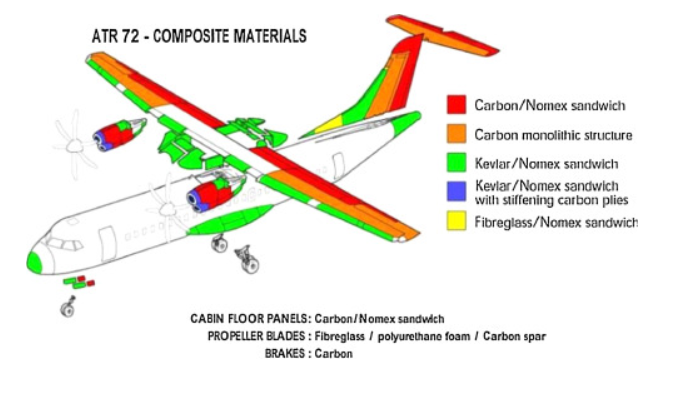
\includegraphics[width=0.75\textwidth]{Images-2-EstudoConceitual/figura1_composito_ATR72.png}
%     \caption{Uso restrito de material compósito no projeto do ATR 72.}
%     \label{fig:composito_atr72}
% \end{figure}

Atualmente, a indústria é dominada por projetos das décadas de 1980 e 1990, como o ATR 72, que possuem limitações arquitetônicas. Diante desse cenário de obsolescência, o desenvolvimento de uma aeronave inteiramente nova, ou "clean sheet", torna-se comercialmente viável e tecnicamente justificado, pois permite a redução substancial do peso vazio operacional através do uso extensivo de compósitos de última geração, por exemplo.

Além disso, um novo design pode viabilizar a integração nativa de sistemas de propulsão híbrida-elétrica e o preparo estrutural para o uso de 100\% de Combustível Sustentável de Aviação (SAF), garantindo conformidade operacional de longo prazo com as cada vez mais rigorosas regulações ambientais.

\subsubsection{O Ambiente Operacional Brasileiro}

No contexto doméstico, o Brasil apresenta um ambiente extremamente favorável, embora logisticamente desafiador, para a introdução dessa nova plataforma. Apesar de o país possuir milhares de municípios e mais de mil aeródromos registrados, apenas 157 localidades recebem voos comerciais regulares, evidenciando que a falta de capilaridade aérea decorre de barreiras de viabilidade econômica das aeronaves atuais e não apenas de limitações de infraestrutura física. 

Essa disparidade regional de acesso aéreo está detalhada espacialmente na Figura~\ref{fig:mapa_acesso} e quantificada na Tabela~\ref{tab:cobertura_aeroportuaria}, revelando  áreas desatendidas nas regiões Norte e Nordeste. 

\begin{figure}[H]
    \centering
    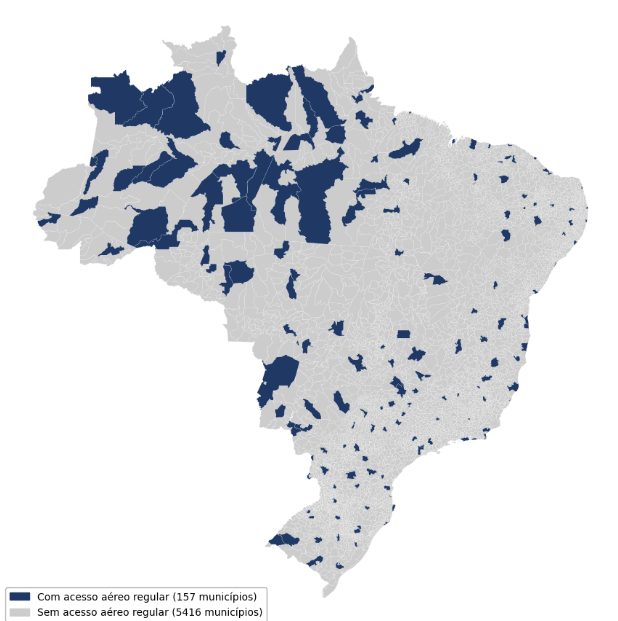
\includegraphics[width=0.6\textwidth]{Images-2-EstudoConceitual/figura2_mapa_coropletico.png}
    \caption{Municípios Brasileiros com e sem Acesso Aéreo Regular (2025).}
    \label{fig:mapa_acesso}
\end{figure}

\begin{table}[H]
\centering
\caption{Cobertura aeroportuária por macrorregião brasileira.}
\label{tab:cobertura_aeroportuaria}
\resizebox{\textwidth}{!}{
\begin{tabular}{l|c|c|c|c}
\hline
\textbf{Região} & \textbf{Municípios} & \textbf{Aeródromos Reg. (ANAC)} & \textbf{Municípios s/ Acesso Aéreo (est.)} & \textbf{Índice de Cobertura (\%)} \\ \hline
Norte & 450 & $\sim$105 & $\sim$375 & $\sim$23\% \\ \hline
Nordeste & 1.794 & $\sim$220 & $\sim$1.574 & $\sim$12\% \\ \hline
Centro-Oeste & 467 & $\sim$180 & $\sim$315 & $\sim$39\% \\ \hline
Sudeste & 1.668 & $\sim$410 & $\sim$1.258 & $\sim$25\% \\ \hline
Sul & 1.191 & $\sim$340 & $\sim$890 & $\sim$29\% \\ \hline
\textbf{Brasil (Total)} & \textbf{5.570} & \textbf{$\sim$1.255} & \textbf{$\sim$4.315} & \textbf{$\sim$22\%} \\ \hline
\end{tabular}
}
\end{table}

Para superar esses gargalos e destravar rotas inéditas, a capacidade do novo projeto de operar em pistas curtas, especificamente com decolagens em 4.200 pés e pousos em 3.000 pés, surge como um diferencial competitivo fundamental. 

O panorama atual do mercado interno é amplamente dominado pela Azul Linhas Aéreas, operadora que baseia suas estratégias em ligar o interior aos grandes centros, um cenário resumido na Tabela~\ref{tab:operadoras_regionais} e ilustrado pelas estatísticas de tráfego histórico de passageiros na Figura~\ref{fig:trafego_pax} e de participação de mercado na Figura~\ref{fig:market_share}. 

\begin{table}[H]
\centering
\caption{Principais operadoras de aviação regional no Brasil (2024).}
\label{tab:operadoras_regionais}
\resizebox{\textwidth}{!}{
\begin{tabular}{l|c|p{3.5cm}|p{3.5cm}|p{4.5cm}}
\hline
\textbf{Operadora} & \textbf{Destinos} & \textbf{Frota Regional} & \textbf{Mercado-Alvo} & \textbf{Observações Relevantes} \\ \hline
Azul Linhas Aéreas & $\sim$160 & ATR 72-600 (aprox. 39 un.) & Cidades médias e pequenas do interior & Maior malha regional do Brasil; opera $\sim$50\% de destinos exclusivos \\ \hline
VoePass (2024) & $\sim$40 & ATR 72-600 e ATR 42-500 & Interior de São Paulo, Sul e Centro Oeste & Possuía operações codeshare com LATAM; foco em rotas não atendidas por jatos \\ \hline
GOL / parceiras & $\sim$100 & Boeing 737 + parcerias & Hubs e alimentação via parceiros & Depende de operadoras menores para capilaridade; sem frota turboélice própria \\ \hline
\end{tabular}
}
\end{table}

\begin{figure}[H]
    \centering
    \begin{minipage}{0.48\textwidth}
        \centering
        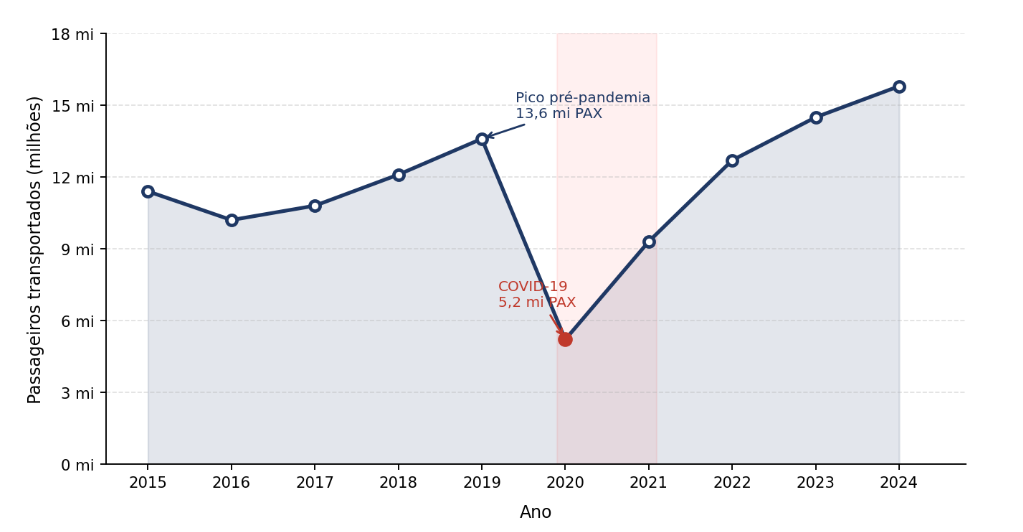
\includegraphics[width=\linewidth]{Images-2-EstudoConceitual/figura3_trafego.png}
        \caption{Tráfego histórico de passageiros na aviação regional brasileira.}
        \label{fig:trafego_pax}
    \end{minipage}
    \hfill
    \begin{minipage}{0.48\textwidth}
        \centering
        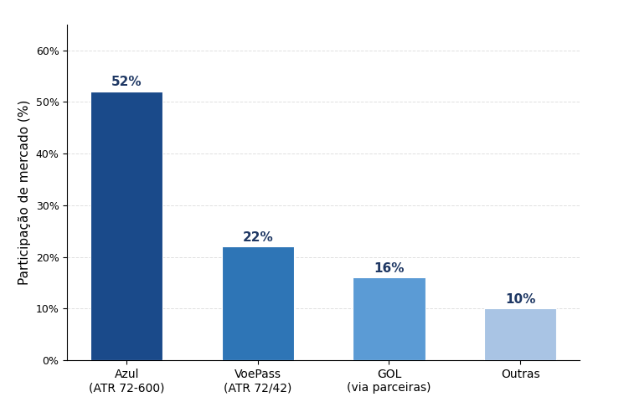
\includegraphics[width=\linewidth]{Images-2-EstudoConceitual/figura4_market_share.png}
        \caption{Participação de mercado das operadoras regionais (2024).}
        \label{fig:market_share}
    \end{minipage}
\end{figure}

Agravando a necessidade de inovação, a frota brasileira de turboélices em operação possui uma média de idade superior a 15 anos, o que catalisa a urgência de um iminente e expressivo ciclo de substituição.

\subsubsection{Conectividade e Demandas Internacionais}

A urgência por aeronaves regionais robustas e eficientes reverbera com igual intensidade em mercados internacionais estratégicos, ampliando o potencial de exportação do projeto. Na África, projeta-se um crescimento anual de tráfego aéreo de 5,1\% até 2043, concentrado em um continente onde a vasta maioria das cidades em desenvolvimento não dispõe de aeroportos com pistas pavimentadas compatíveis com jatos de médio porte. 

Similarmente, a macrorregião da Ásia-Pacífico lidera o ritmo de crescimento global do setor, impulsionada por políticas governamentais de interiorização do transporte na Índia (programa UDAN) e pela geografia arquipelágica da Indonésia, onde a expressiva economia de combustível dos turboélices é vital para viabilizar as ligações inter-ilhas. Em uma dinâmica diferente, mas complementar, o mercado maduro dos Estados Unidos demandará na próxima década a substituição direta de cerca de 800 jatos regionais defasados que alimentam seus complexos hubs, consolidando uma lógica de distribuição de tráfego que corrobora a utilidade universal de um avião regional moderno.

Essa convergência global de demandas e a necessidade latente de renovação de frota refletem-se de maneira contundente nas previsões para as próximas duas décadas. Como sumarizado na Tabela~\ref{tab:previsao_mercado} e ilustrado na Figura~\ref{fig:entregas_regionais}, a indústria aeronáutica projeta a entrega constante e volumosa de novas unidades para suprir a conectividade de curto e médio alcance.

\begin{table}[H]
\centering
\caption{Previsões de mercado para aeronaves regionais (50-90 assentos), 2024-2043.}
\label{tab:previsao_mercado}
\resizebox{\textwidth}{!}{
\begin{tabular}{l|c|c|p{4cm}|p{3.5cm}}
\hline
\textbf{Região / Segmento} & \textbf{Previsão de Entregas} & \textbf{Crescimento PAX} & \textbf{Déficit de Infraestrutura} & \textbf{Fonte} \\ \hline
América Latina (total) & $\sim$750 aeronaves & 4,5\% / ano & Poucas pistas pavimentadas & ATR Market Forecast 2024 \\ \hline
Brasil ($<$ 90 PAX) & $\sim$200-250 aeronaves & 3,8\% / ano & 4.300+ municípios sem acesso regular & ANAC / Embraer CMO 2024 \\ \hline
África Subsaariana & $\sim$450 aeronaves & 5,1\% / ano & Modal aéreo único em vastas regiões & IATA Industry Statistics 2024 \\ \hline
América do Norte & $\sim$800 aeronaves & 2,2\% / ano & Sistema hub-and-spoke maduro & FAA Aerospace Forecast 2024 \\ \hline
Ásia-Pacífico (incl. China) & $\sim$1.045 aeronaves & 5,2\% / ano & Geografia arquipelágica e cidades Tier 2/3 & ATR GMF / IATA \\ \hline
Oceania (incl. Austrália) & $\sim$125 aeronaves & 4,1\% / ano & Vastas distâncias e renovação de frota & Embraer CMO / Qantas \\ \hline
\end{tabular}
}
\end{table}

\begin{figure}[H]
    \centering
    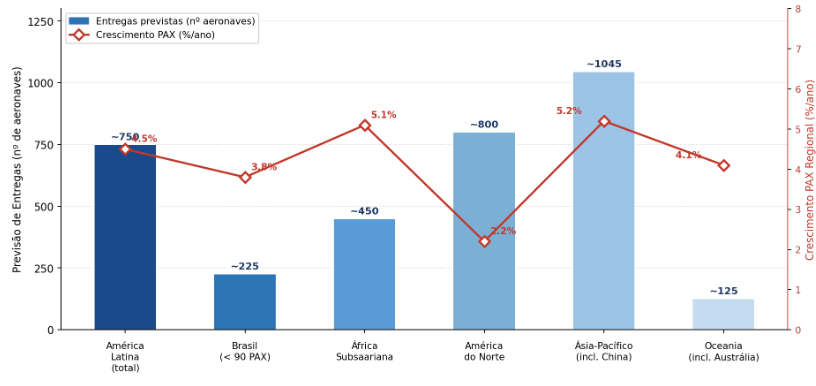
\includegraphics[width=0.85\textwidth]{Images-2-EstudoConceitual/figura6_entregas.png}
    \caption{Previsão global de entregas de aeronaves regionais (50-90 PAX) por região entre 2024 e 2043.}
    \label{fig:entregas_regionais}
\end{figure}

\subsection{Transporte de Cargas}

\subsubsection{Impacto do \textit{e-commerce}}

O setor que mais alavanca o transporte aéreo mundial de cargas é o e-commerce, com previsão de receita de mais de 6,4 trilhões de dólares para 2029, segundo dados da Statista Market Insights. No Brasil, a tendência de crescimento desse setor se mantém, sendo uma das maiores de todo o mundo, tal que uma pesquisa internacional da Insider Intelligence colocou o país entre os 10 com mais expectativa de crescimento do \textit{e-commerce} em 2022. Além disso, segundo a ABComm (Associação Brasileira de Comércio Eletrônico), a previsão para essa modalidade é um crescimento de 10\% ao ano até 2029, sem contar que, apenas para 2026, já prevê um número de 2 milhões de novos compradores \cite{gazetadopovo2026}.

Nesse sentido, gigantes do setor têm investido em malhas aéreas próprias para garantir diferenciais competitivos. A Amazon Air, por exemplo, registrou um crescimento de 102\% no número de voos diários entre 2020 e 2022. Paralelamente, o Mercado Livre (MELI AIR) expandiu sua frota visando reduzir o tempo de entrega nas capitais do Norte e Nordeste para apenas um dia. Esta tendência de crescimento nas entregas de compras pela internet reforça a necessidade de aeronaves regionais versáteis para essas operações \cite{gazetadopovo2026}.

\subsubsection{Matriz de Transporte Brasileira}

No cenário nacional, o modal aéreo apresenta uma participação de apenas 0,05\% do total de toneladas-quilômetros úteis (TKUs) movimentados, contrastando com os mais de 60\% do modal rodoviário. No entanto, esta baixa representatividade em volume bruto é paradoxal ao valor, já que o setor movimenta mercadorias de altíssimo valor agregado e urgência. Em 2022, o Brasil atingiu o seu recorde histórico de volume movimentado, totalizando 1,421 milhões de toneladas, com um aumento de 0,7\% em carga paga doméstica e 4,3\% em correios com relação ao ano anterior, conforme apresentado na Figura \ref{volume transportado de cargas}. Estes dados validam a existência de uma possível demanda por uma aeronave de médio porte, focada no transporte de bens nos quais a segurança e a rapidez justificam o custo do frete \cite{aeroincarga2026}.

\begin{figure} [H]
    \centering
    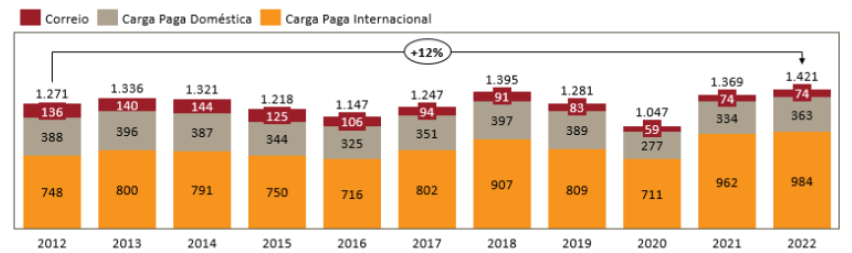
\includegraphics[width=0.9\linewidth]{images/Série histórica de transporte - Brasil.png}
    \caption{Série histórica do volume transportado de cargas pelo modal aéreo no Brasil, de 2012 a 2022 \cite{mercadolivre2022}.} 
    \label{volume transportado de cargas}
    
\end{figure}

Além disso, um ponto a ser levado em consideração são as principais rotas domésticas para transporte de cargas via modal aéreo no Brasil. Entre essas rotas, as quatro principais envolvem o aeroporto de Manaus (SBEG) e os aeroportos do estado de São Paulo – Guarulhos (SBGR) e Campinas (SBKP). O elevado fluxo aéreo entre estas duas regiões acontece pelo fato de Manaus ser uma região remota, com pouca estrutura rodoviária, porém que fabrica produtos de alto valor agregado por meio da Zona Franca de Manaus. Já o estado de São Paulo é o principal centro econômico do país, logo, consome grande parte das tecnologias que são produzidas na Zona Franca \cite{almeida2016}. 

Conforme retratado já na Figura \ref{fig:entregas_regionais} e explicado na seção anterior, o território brasileiro conta com uma deficiência em relação ao número de localidades com acesso aéreo regular. Dessa maneira, para poder utilizar os milhares de aeródromos registrados no Brasil para transportar cargas e, portanto, agilizar a logística no transporte de mercadorias em território nacional, há uma exigência de operação para pistas curtas de 4.200 ft (decolagem) e 3.000 ft (pouso).

Uma região altamente dependente dessa exigência técnica é o norte do país, de modo que, por possuir uma estrutura rodoviária precária, depende criticamente do modal aéreo. Alinhado ao que foi mencionado em relação ao fluxo concentrado entre Manaus (SBEG) e São Paulo (Guarulhos e Campinas), fica clara a necessidade de aeronaves operando nessa rota.

Além disso, a aviação regional constitui o elo vital entre estes grandes \textit{hubs} e cidades de médio porte. Estudos reforçam que pequenos aeroportos regionais impulsionam o desenvolvimento econômico local, mas enfrentam dificuldades para cobrir custos operacionais. Frotas eficientes com capacidades STOL (\textit{Short Take-Off and Landing}) e baixo custo operacional (DOC) são, portanto, a solução técnica para tornar estas rotas economicamente autossustentáveis.

\subsubsection{Conectividade e Demandas Internacionais}

Segundo a análise dos dados apresentados no \textit{Boeing World Air Cargo Forecast} \cite{boeing2024wacf}, projeta-se um cenário de resiliência e expansão para o setor de logística aérea nas próximas duas décadas, de modo que o mercado é caracterizado por um crescimento anual composto (CAGR) de 4,0\%, impulsionado pela digitalização do comércio global e pela reestruturação das cadeias de suprimentos. Além disso, um dos pontos mais relevantes para a análise de mercado é a composição da frota futura, estimada em 3.900 aeronaves até 2043.

No curto prazo, os dados de 2025 da pesquisa de \textit{Global Market Forecast} da Airbus \cite{airbus2025gmf} corroboram essa tendência de alta, registrando um crescimento mundial de 3,3\% no acumulado até agosto, apesar do desempenho regional heterogêneo, conforme apresentado na Figura \ref{fig:tráfego mundial de carga}.

\begin{figure} [H]
    \centering
    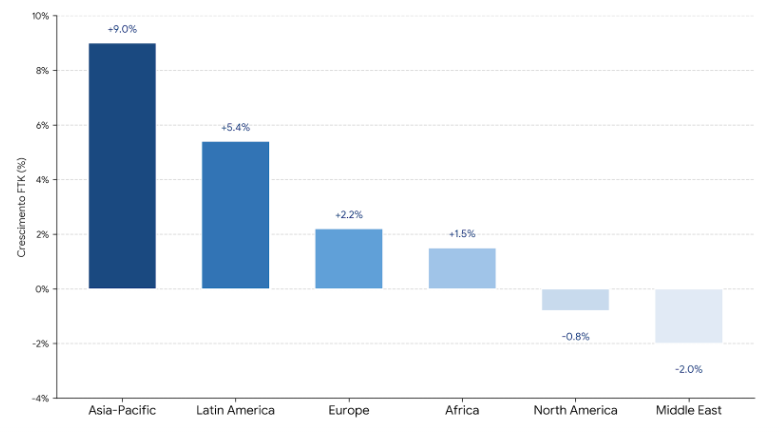
\includegraphics[width=0.8\linewidth]{images/Tráfego Mundial de Carga.png}
    \caption{Crescimento do tráfego de carga aérea por região (Jan - Ago 2025) \cite{airbus2025gmf}}
    \label{fig:tráfego mundial de carga}
\end{figure}

Por fim, é prevista uma consolidação de 25\% do \textit{share} para transportadoras expressas (como FedEx, DHL, UPS) até 2043, sendo esse um reflexo direto da irreversibilidade do \textit{e-commerce} transfronteiriço, o qual exige aeronaves com alta disponibilidade e ciclos rápidos, influenciando o \textit{design} de redes logísticas e a demanda por aeronaves de médio porte (\textit{narrow-body}) para alimentação de \textit{hubs} regionais. Nesse sentido, o mercado de carga aérea caminha para uma maior autonomia em relação ao transporte de passageiros. Para empresas do setor, o foco deve estar na eficiência operacional em mercados emergentes e na capacidade de execução de conversões de frota.

% --- SEÇÃO DE ESTUDO COMPARATIVO ---

\section{Estudos Comparativos}
\label{sec:estudoscomparativos}
O desenvolvimento do projeto conceitual é fundamentado em uma análise detalhada de aeronaves que operam no mesmo segmento ou que possuem características técnicas similares aos requisitos da seção~\ref{section:Requisitos}. Inicialmente, foram selecionadas 23 aeronaves, abrangendo uma ampla gama de modelos regionais, cargueiros e militares, com o intuito de estabelecer uma base para o esboço da geometria inicial.

A seleção baseou-se em parâmetros fundamentais como o Peso Máximo de Decolagem (MTOW), capacidade de passageiros, alcance e desempenho em pista \cite{medeiros2026}. A Tabela \ref{tab:comparativo_completo} apresenta os parâmetros básicos e essenciais dessas aeronaves, conforme levantamento realizado pelo grupo.


\begin{table}[H]
\centering
\caption{Levantamento abrangente de todas as aeronaves pesquisadas para análise estatística inicial.}
\label{tab:comparativo_completo}
\resizebox{\textwidth}{!}{%
\begin{tabular}{l|c|c|c|c|c|c}
\hline
\textbf{Modelo} & \textbf{Pax} & \textbf{MTOW [kgf]} & \textbf{$V_{cruise}$ [kt]} & \textbf{Alcance [nm]} & \textbf{Teto [ft]} & \textbf{Pista DE/PO [m]} \\ \hline
CASA C-295 & 71 & 21.000 & 260 & 3.040 & 30.000 & 978 / 789 \\ \hline
ATR 72-600 & 70-78 & 22.800 & 275 & 825 & 25.000 & 1.410 / 915 \\ \hline
Bombardier Dash 8 Q400 & 70-86 & 29.257 & 360 & 1.362 & 25.000 & 1.402 / 1.134 \\ \hline
Ilyushin Il-114-300 & 68 & 23.500 & 243 & 756 & 25.000 & 1.160 / 610 \\ \hline
NAMC YS-11 & 64 & 22.900 & 253 & 1.188 & 23.000 & 1.100 / 660 \\ \hline
BAe ATP & 64-70 & 22.930 & 268 & 985 & 25.000 & 1.460 / 1.130 \\ \hline
Saab 2000 & 50-58 & 22.999 & 370 & 1.549 & 31.000 & 1.355 / 1.200 \\ \hline
Antonov An-140-100 & 52 & 21.500 & 310 & 1.997 & 24.900 & 1.750 / 1.400 \\ \hline
Xian MA600 & 60 & 21.800 & 278 & 891 & 25.000 & 1.800 / 1.600 \\ \hline
Fokker 50 & 50 & 20.820 & 284 & 1.200 & 25.000 & 1.305 / 1.215 \\ \hline
Antonov An-26 & 40 & 24.000 & 237 & 1.300 & 24.600 & - / - \\ \hline
Leonardo C-27J Spartan & 62 & 32.500 & 325 & 3.160 & 30.000 & 690 / 390 \\ \hline
Short 360 "The Shed" & 36 & 12.292 & 212 & 915 & 20.000 & 1.158 / 853 \\ \hline
Mitsubishi SpaceJet (MRJ70) & 80 & 40.200 & 542 & 2.019 & 41.000 & 1.720 / 1.430 \\ \hline
Embraer ERJ 145 & 54 & 19.200 & 520 & 1.550 & 37.000 & 1.380 / 1.400 \\ \hline
Comac ARJ21-700 & 90 & 43.500 & 529 & 3.668 & 39.000 & 1.900 / 1.650 \\ \hline
Antonov An-148 & 92 & 43.700 & 470 & 1.275 & 40.000 & 1.685 / - \\ \hline
Transall C-160 & 93 & 51.000 & 320 & 4.780 & 27.000 & 730 / 550 \\ \hline
Embraer E190 & 104 & 47.790 & 547 & 2.850 & 41.000 & 1.267 / 1.244 \\ \hline
Saab 340F & 33-37 & 13.155 & 283 & 1.732 & 25.000 & 1.220 / 1.035 \\ \hline
Embraer EMB 110 & 18 & 5.788 & 236 & 1.118 & 21.000 & 380 / 400 \\ \hline
Cessna SkyCourier & 19 & 8.618 & 210 & 920 & 25.000 & 3.660 / 3.010 \\ \hline
Dornier Do 228 & 19 & 6.400 & 223 & 1.340 & 25.000 & 792 / 451 \\ \hline
\end{tabular}%
}
\end{table}

Após a avaliação, muitas aeronaves foram excluídas da análise por apresentarem divergências significativas em relação aos requisitos de missão estipulados para este projeto, a saber \cite{medeiros2026}:

\begin{itemize}
    \item \textbf{Propulsão e Regime de Velocidade:} Aeronaves equipadas com motores turbofan (ERJ 145, E190, SpaceJet, Antonov An-148) foram descartadas por operarem em velocidades de cruzeiro e altitudes muito superiores ao requisito de $260 \text{ kt}$ e $FL250$ \cite{medeiros2026}.
    \item \textbf{Porte e Capacidade:} Modelos como o Cessna SkyCourier, EMB 110 e Dornier 228, embora turboélices, possuem capacidade inferior a 20 passageiros, distanciando-se do requisito de 60 a 70 ocupantes \cite{medeiros2026}.
    \item \textbf{Missão e MTOW:} Aeronaves como o Transall C-160 e o Leonardo C-27J foram excluídas devido ao perfil de missão estritamente militar ou MTOW que excede o limite estabelecido de $50.000 \text{ lb}$ \cite{medeiros2026}.
\end{itemize}

Com base nestes critérios, as aeronaves selecionadas para compor a análise comparativa detalhada e fundamentar o Projeto Conceitual são: \textbf{ATR 72-600}, \textbf{CASA C-295}, \textbf{Ilyushin Il-114-300}, \textbf{BAe ATP}, \textbf{NAMC YS-11} e \textbf{Xian MA600}. Estas aeronaves representam os competidores diretos, conciliando a configuração turboélice, capacidade de passageiros e peso máximo de decolagem exigidos pelo projeto \cite{medeiros2026}. A Tabela \ref{tab:competidores_geometria} detalha os parâmetros geométricos e de desempenho dos modelos selecionados. 

\begin{table}[h!]
\centering
\caption{Parâmetros das aeronaves de referência selecionadas.}
\label{tab:competidores_geometria}
\resizebox{\textwidth}{!}{%
\begin{tabular}{l|c|c|c|c|c|c}
\hline
\textbf{Parâmetro} & \textbf{ATR 72-600} & \textbf{CASA C-295} & \textbf{Il-114-300} & \textbf{BAe ATP} & \textbf{NAMC YS-11} & \textbf{Xian MA600} \\ \hline
MTOW [kgf] & 22.800 & 21.000 & 23.500 & 23.700 & 22.900 & 21.800 \\ \hline
Área Alar [$m^2$] & 61,00 & 59,00 & 81,90 & 78,30 & 94,83 & 75,00 \\ \hline
Envergadura [m] & 27,05 & 25,81 & 29,87 & 30,63 & 32,00 & 29,20 \\ \hline
Nome do Motor & PW127M & PW127G & TV7-117ST-01 & PW126A & RR Dart Mk.542 & PW127J \\ \hline
Potência [shp] & 4.950 & 5290 & 5300 & 5306 & 5320 & 5762 \\ \hline
$V_{cruise}$ [kt] & 275 & 260 & 243 & 268 & 253 & 278 \\ \hline
$V_{stall}$ [kt] & 87 & 75-80 & 87 & 86 & 76 & 75 \\ \hline
Compr. Cabine [m] & 17,00 & 12,69 & 18,93 & 19,20 & 17,00 & 10,80 \\ \hline
Largura Cabine [m] & 2,57 & 2,70 & 2,64 & 2,48 & 2,70 & 2,70 \\ \hline
Altura Cabine [m] & 1,91 & 1,90 & 1,92 & 1,92 & 1,90 & 1,90 \\ \hline
Razão de Subida [ft/min] & 1.355 & 700 & 1000 & 1.000 & 1.220 & 1.500 \\ \hline
$N^\circ$ de Lugares & 70-78 & 71 & 68 & 64-70 & 64 & 60 \\ \hline
Alcance [nm] & 825 & 730 & 756 & 985 & 1.188 & 891 \\ \hline
Dist. Decolagem [m] & 1.410 & 978 & 1.160 & 1.460 & 1.100 & 1.800 \\ \hline
Dist. Pouso [m] & 915 & 789 & 610 & 1.130 & 660 & 1.600 \\ \hline
\end{tabular}%
}
\end{table}

\subsection{Configuração de Asa}

Para uma aeronave que deve cumprir missões de transporte regional de passageiros e de cargas a relativa baixa velocidade, a escolha de uma configuração de asa que permita bom desempenho em aerodinâmica e estabilidade, além da viabilidade operacional em aeroportos de menor infraestrutura é de suma importância.

Em primeira análise, a escolha entre uma asa alta, média ou baixa seria o primeiro passo, visto que cada uma por si só já trás características bem diferentes para os aspectos mencionados no parágrafo acima. De acordo com Anderson \cite{anderson1999}, uma asa alta favorece a capacidade operacional ao permitir que a fuselagem fique mais próxima do solo, permitindo cargas e descargas mais rápidas e com menos complexidade logística. Além disso, a asa alta tem um efeito estabilizante lateralmente muito forte, sendo, às vezes, necessário impor um diedro negativo (anedro) para aumentar a capacidade de rolamento da aeronave, por exemplo. Outro aspecto bastante positivo é que a asa alta fica longe do solo, permitindo motores maiores (no caso de \textit{turbofans}) e hélices maiores (no caso de motores convencionais ou turbohélices) sem a necessidade de uma estrutura que eleve a posição do motor (que aumentaria peso da aeronave).

Anderson \cite{anderson1999} explica também que asas médias são boas principalmente em questão de arrasto, visto que minimiza a interferência asa-fuselagem, porém pecam muito devido a necessidade de reforço estrutural na fuselagem e complicação para passagem de passageiros e/ou cargas.

Finalmente, asas baixas são boas em aproveitar o efeito solo (melhorando desempenho em pouso e decolagem). Porém, elas exigem que a fuselagem seja colocada numa altura maior do solo para permitir o posicionamento de motores/hélices. Além de que essa altura significa que o trem de pouso deve ser maior e consequentemente mais peso. \cite{anderson1999}

Tratando das características da asa em si, partimos de diversos parâmetros, como alongamento (\textit{Aspect Ratio - $AR$}), afilamento ($\lambda$), diedro ($\Gamma$), enflechamento no bordo de ataque ($\Lambda_{LE}$), a um quarto de corda ($\Lambda_{c/4}$), ângulo de incidência ($i_w$), entre outros.

O alongamento impacta em muitas características. Em geral, quanto maior o alongamento, melhor a eficiência ($L/D$) da asa, menor arrasto induzido, maior derivada $C_{L_\alpha}$, porém possui um amortecimento muito grande em relação ao rolamento, a asa é mais sucetível à flexão e a velocidade de \textit{flutter} é menor. Já asas pouco alongadas possuem ângulo de stall maior e menor peso estrutural. Porém possuem maior arrasto induzido, menor $C_{L_{max}}$ e propriedades aerodinâmicas de modo geral ruins para baixas velocidades \cite{gudmundsson2021}

Em relação ao afilamento (\textit{Taper Ratio}), a escolha normalmente está relacionada a um balanço entre característica de \textit{stall} e arrasto induzido. \cite{gudmundsson2021}

No que se trata do diedro, ele pode aumentar a estabilidade lateral da aeronave (diedro positivo) ou diminuir (anedro). Nesse sentido, o diedro positivo é  utilizado nas aeronaves comerciais para garantir voos mais estáveis e seguros, enquanto que o anedro é usado normalmente em projetos com asa alta ou com asas muito enflechadas, a fim de reduzir a força restauradora excessiva, preservando a manobrabilidade.

Já o ângulo de incidência da asa é, conforme Gudmundsson \cite{gudmundsson2021}, estabelecido primariamente para reduzir o arrasto em cruzeiro, pois permite que a asa opere no ângulo de ataque ótimo dessa fase enquanto a fuselagem se mantém alinhada ao escoamento (ângulo de ataque próximo de zero), evitando que esta gere arrasto adicional por operar fora de sua condição aerodinâmica ideal.

Por fim, o ângulo de enflechamento é normalmente utilizado por dois motivos principais: o posicionamento do centro de gravidade (CG) e a redução do arrasto de onda de choque em voos transônicos e supersônicos.


\subsection{Configuração das Empenagens}

A determinação da geometria das empenagem foi baseada, inicialmente, na análise dos coeficientes de volume de cauda. O coeficiente de volume de cauda horizontal é definido como:

\begin{equation}
V_{HT} = \frac{l_{HT} S_{HT}}{\bar{c} S}
\end{equation}

e o coeficiente de volume de cauda vertical como:

\begin{equation}
V_{VT} = \frac{l_{VT} S_{VT}}{b S}
\end{equation}

onde $l_{HT}$ e $l_{VT}$ são as distâncias entre o centro de gravidade da aeronave e os centros aerodinâmicos das respectivas superfícies, $S_{HT}$ e $S_{VT}$ são as áreas da empenagem horizontal e vertical, $\bar{c}$ é a corda média aerodinâmica da asa, $b$ é a envergadura da asa e $S$ é a área da asa \cite{anderson1999}. Esses coeficientes representam uma medida adimensional da capacidade das empenagens em gerar momentos estabilizantes, dentre outros.

No que diz respeito à configuração geométrica, existem diferentes arranjos possíveis para as empenagens, sendo os mais comuns a configuração convencional, a configuração em T e a configuração cruciforme. A configuração convencional, na qual a empenagem horizontal é posicionada na base da empenagem vertical (ou diretamente na fuselagem), é a mais utilizada, estando presente na maioria das aeronaves devido à  simplicidade estrutural, menor peso e bom compromisso entre estabilidade e controle.

Já configuração em T posiciona a empenagem horizontal no topo da empenagem vertical, trazendo algumas vantagens aerodinâmicas, como a redução da interferência com a esteira da asa. No entanto, apresenta desvantagens estruturais significativas, exigindo reforços pesados na empenagem vertical.

Já a configuração cruciforme representa um compromisso entre as duas anteriores, posicionando a empenagem horizontal em uma posição intermediária na empenagem vertical, buscando equilibrar os benefícios aerodinâmicos e estruturais \cite{anderson1999}.

O posicionamento longitudinal das empenagens resulta de um compromisso entre ganho de autoridade e aumento de peso estrutural. Em geral, busca-se posicionar a cauda mais afastada do centro de gravidade para aumentar o braço de alavanca ($l_{HT}$ e $l_{VT}$), reduzindo a área necessária das superfícies para um mesmo efeito estabilizante. Entretanto, esse aumento do braço também exige uma fuselagem estruturalmente mais robusta e, consequentemente, mais pesada, devendo ambos os efeitos ser balanceados no projeto \cite{anderson1999}.


\subsection{Configuração de Cabine}

O dimensionamento interno da fuselagem é tradicionalmente realizado por meio de um processo de dentro para fora, no qual a cabine de passageiros e o compartimento de carga determinam a geometria das seções transversal e longitudinal, posteriormente refinada com base em critérios aerodinâmicos externos \cite{raymer2018}. Para esta aeronave, projetada para acomodar entre 60 e 70 passageiros, a prioridade é atender aos requisitos de conforto, ergonomia e flexibilidade de missão.


A cabine adotará uma configuração de 4 assentos por fileira (2+2), separados por um corredor central, o que representa o padrão da indústria para turboélices regionais deste porte. Além disso, o projeto prevê trilhos estruturais no piso para permitir a rápida conversão entre a configuração de passageiros e o transporte de carga utilizando ULDs, contêineres e pallets padronizados. A porta principal de carga será dimensionada para permitir a passagem desses dispositivos, respeitando as normas internacionais para operações logísticas.

A fim de balizar as dimensões principais da fuselagem (comprimento, largura e altura interna), realizou-se uma análise estatística dos seis concorrentes diretos aprovados na filtragem do Projeto Conceitual. Os resultados deste comparativo estão expressos nas Figuras \ref{fig:bar_comp_cabine}, \ref{fig:bar_largura_cabine} e \ref{fig:bar_altura_cabine}.

\begin{figure}[H]
    \centering
    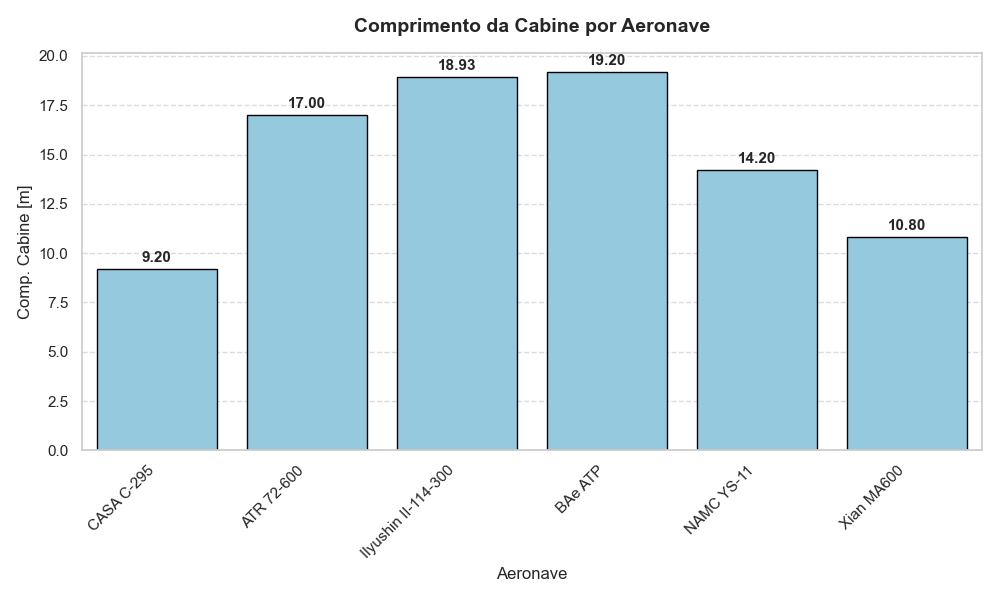
\includegraphics[width=0.75\linewidth]{Images-2-EstudoConceitual/Comp_cabine.png} % Ajuste o caminho se necessário
    \caption{Comparativo do comprimento da cabine entre as aeronaves de referência.}
    \label{fig:bar_comp_cabine}
\end{figure}

\begin{figure}[H]
    \centering
    \begin{minipage}{0.48\textwidth}
        \centering
        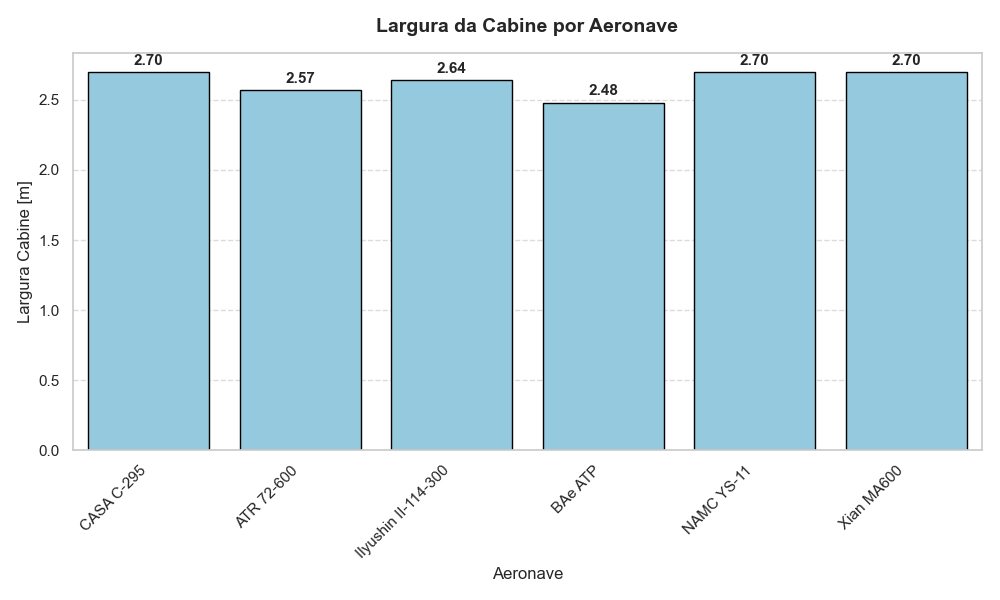
\includegraphics[width=\linewidth]{Images-2-EstudoConceitual/Larg_cabine.png} % Ajuste o caminho se necessário
        \caption{Largura interna da cabine.}
        \label{fig:bar_largura_cabine}
    \end{minipage}
    \hfill
    \begin{minipage}{0.48\textwidth}
        \centering
        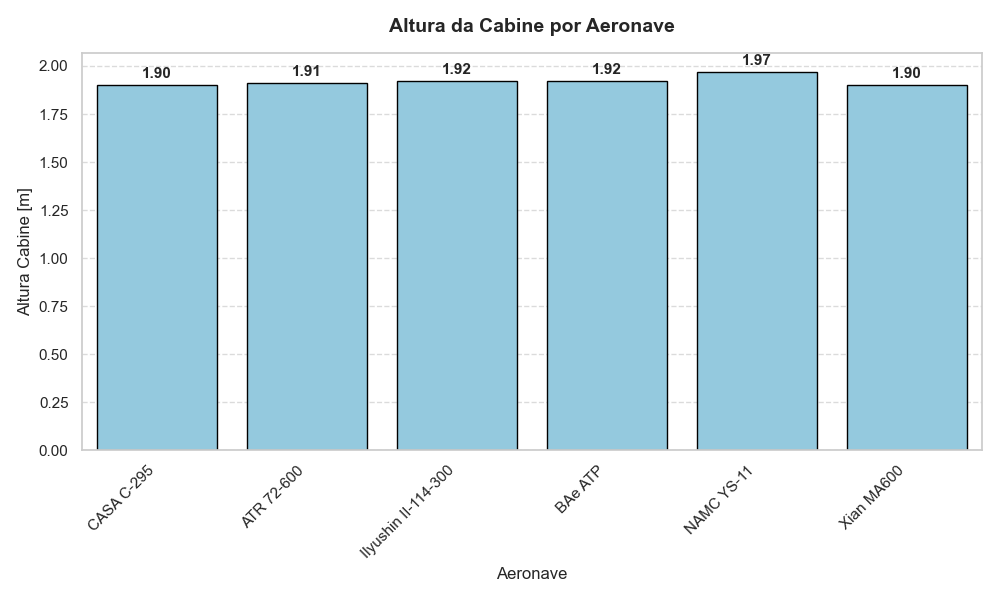
\includegraphics[width=\linewidth]{Images-2-EstudoConceitual/Alt_cabine.png} % Ajuste o caminho se necessário
        \caption{Altura interna da cabine.}
        \label{fig:bar_altura_cabine}
    \end{minipage}
\end{figure}

A análise da Figura \ref{fig:bar_comp_cabine} revela uma variância significativa no comprimento da cabine em função do perfil da missão. O modelo CASA C-295 apresenta um valor nitidamente inferior (9,20 m) por ser uma aeronave de origem militar. Em contrapartida, as aeronaves dedicadas primariamente ao transporte civil de passageiros (como o ATR 72, Il-114 e YS-11) agrupam-se na faixa de 14,00 m a 19,00 m. Para acomodar as fileiras de assentos com o \textit{pitch} (espaçamento) padrão da classe, adicionando espaço para \textit{galleys} (copa) e lavatórios, o Projeto Conceitual adotará um comprimento de cabine em torno de 17,00 m.

Quanto à seção transversal, as Figuras \ref{fig:bar_largura_cabine} e \ref{fig:bar_altura_cabine} demonstram uma forte padronização de mercado. A altura interna varia em uma margem muito estreita (entre 1,90 m e 1,97 m), dimensão estritamente necessária para garantir a ergonomia e permitir que um passageiro adulto do percentil 95 caminhe ereto pelo corredor. 

A largura interna concentra-se entre 2,48 m e 2,70 m, o que é suficiente para acomodar confortavelmente dois assentos duplos (com largura média de 1,00 m a 1,05 m cada par) e um corredor central normativo de no mínimo 0,45 m. 

\subsection{Configuração de Propulsão}

A definição da configuração de propulsão da aeronave foi baseada nos estudos comparativos apresentados. Para a aeronave em estudo, cuja velocidade de cruzeiro máxima é de aproximadamente 260 kt, observa-se que este regime de voo está abaixo da faixa em que motores do tipo turbofan apresentam maior eficiência. Motores turbofan são mais adequados para aeronaves que operam em velocidades mais elevadas e maiores altitudes, nas quais os ganhos associados à propulsão a jato se tornam mais significativos. Em contrapartida, em regimes de baixa a média velocidade, típicos da aviação regional, os motores turboélice apresentam melhor eficiência propulsiva, resultando em menor consumo de combustível para a mesma missão.

Quanto aos motores alternativos, eles apresentam três limitações intrínsecas que dificultam o uso em aeronaves de maior porte. A relação potência-peso é desfavorável, pois o aumento de potência exige mais cilindrada e por consequência um aumento grande de massa. A eficiência cai com a altitude, já que motores aspirados dependem da densidade do ar admitido, perdendo potência conforme a aeronave sobe, limitação que a turbina, com sua razão de compressão interna, não sofre na mesma intensidade, esse problema poderia ser parcialmente resolvido com turbocompressores ou turbonormalizadores, mas no fim existirá ainda mais aumento de peso. Por fim, a vida útil entre revisões é menor, consequência direta da maior quantidade de peças móveis sujeitas a desgaste e fadiga (válvulas, anéis, ignição), o que aumenta a frequência de manutenção em comparação ao turboélice.

Além da eficiência em cruzeiro, os motores turboélice apresentam vantagens operacionais importantes para o perfil da aeronave proposta. Entre elas, destacam-se a melhor performance em decolagens e pousos em pistas curtas, maior eficiência em altitudes moderadas e maior robustez para operações em aeroportos com infraestrutura limitada. Tais características são particularmente relevantes considerando os requisitos de operação da aeronave, que incluem pistas de comprimento reduzido e voos regionais de curta e média distância.

Outro fator determinante é o custo operacional. Motores turboélice, em geral, apresentam menor consumo específico de combustível em regimes subsônicos baixos e, apesar de um custo mais elevado no ciclo de manutenção, são mais baratos. 

No que se refere à redundância e segurança operacional, a adoção de uma configuração bimotor é considerada essencial. Essa configuração permite que a aeronave mantenha capacidade de voo segura mesmo em caso de falha de um dos motores, atendendo aos requisitos de certificação e ampliando a flexibilidade operacional, especialmente em rotas que envolvem regiões com infraestrutura limitada. 

Dessa forma, a configuração bimotor turboélice foi selecionada como a mais adequada para a aeronave em estudo, proporcionando um equilíbrio entre eficiência em cruzeiro, desempenho em operações de pista curta, custos operacionais e segurança, atendendo de forma consistente às exigências das missões de transporte regional de passageiros e carga.

\subsection{Configuração do Trem de Pouso}

Adotou-se a geometria de trem de pouso triciclo retrátil, configuração que representa o padrão da indústria para aeronaves comerciais modernas por garantir estabilidade direcional superior durante o táxi e facilitar as operações de pouso e decolagem, além de ser o caso de todas as aeronaves mencionadas na tabela \ref{tab:competidores_geometria}.

Para a absorção de impactos, a engenharia consolidou arquiteturas distintas. Os amortecedores óleo-pneumáticos com tesoura de torção, ilustrados na Figura \ref{fig:oleopneumatic}, utilizam a compressibilidade do nitrogênio como mola pneumática para suportar o peso estático e o óleo hidráulico para dissipar a energia do impacto através de um orifício medidor. Outra solução complexa é o braço arrastado (\textit{trailing link}), apresentado na Figura \ref{fig:TrailingArm}, que utiliza um braço articulado atuando como alavanca para proporcionar uma compressão mais progressiva do amortecedor, sendo excepcionalmente eficaz na absorção de cargas verticais e horizontais em pistas irregulares ou pousos de alta energia.

Embora soluções simplificadas como a lâmina de aço mola ou cordas elásticas (\textit{bungee cords}) sejam elegantes pela baixa complexidade, elas apresentam amortecimento limitado e propensão a saltos (\textit{bounces}) em pousos mais bruscos. Tais arquiteturas são restritas a aeronaves leves ou de treinamento e não são viáveis para a classe de peso de 50.000 lb deste projeto. 

Devido à configuração de asa alta, o trem de pouso principal será recolhido em carenagens laterais fixadas na fuselagem. Esta escolha preserva a integridade estrutural da asa e permite que o piso da aeronave permaneça baixo e nivelado, otimizando o carregamento de carga e o acesso de passageiros. Os amortecedores selecionados serão do tipo óleo-pneumático, dimensionados para suportar as cargas operacionais de uma aeronave regional de médio porte.

\begin{figure}[H]
    \centering
    % Primeira figura - Óleo-Pneumático
    \begin{minipage}{0.3\textwidth}
        \centering
        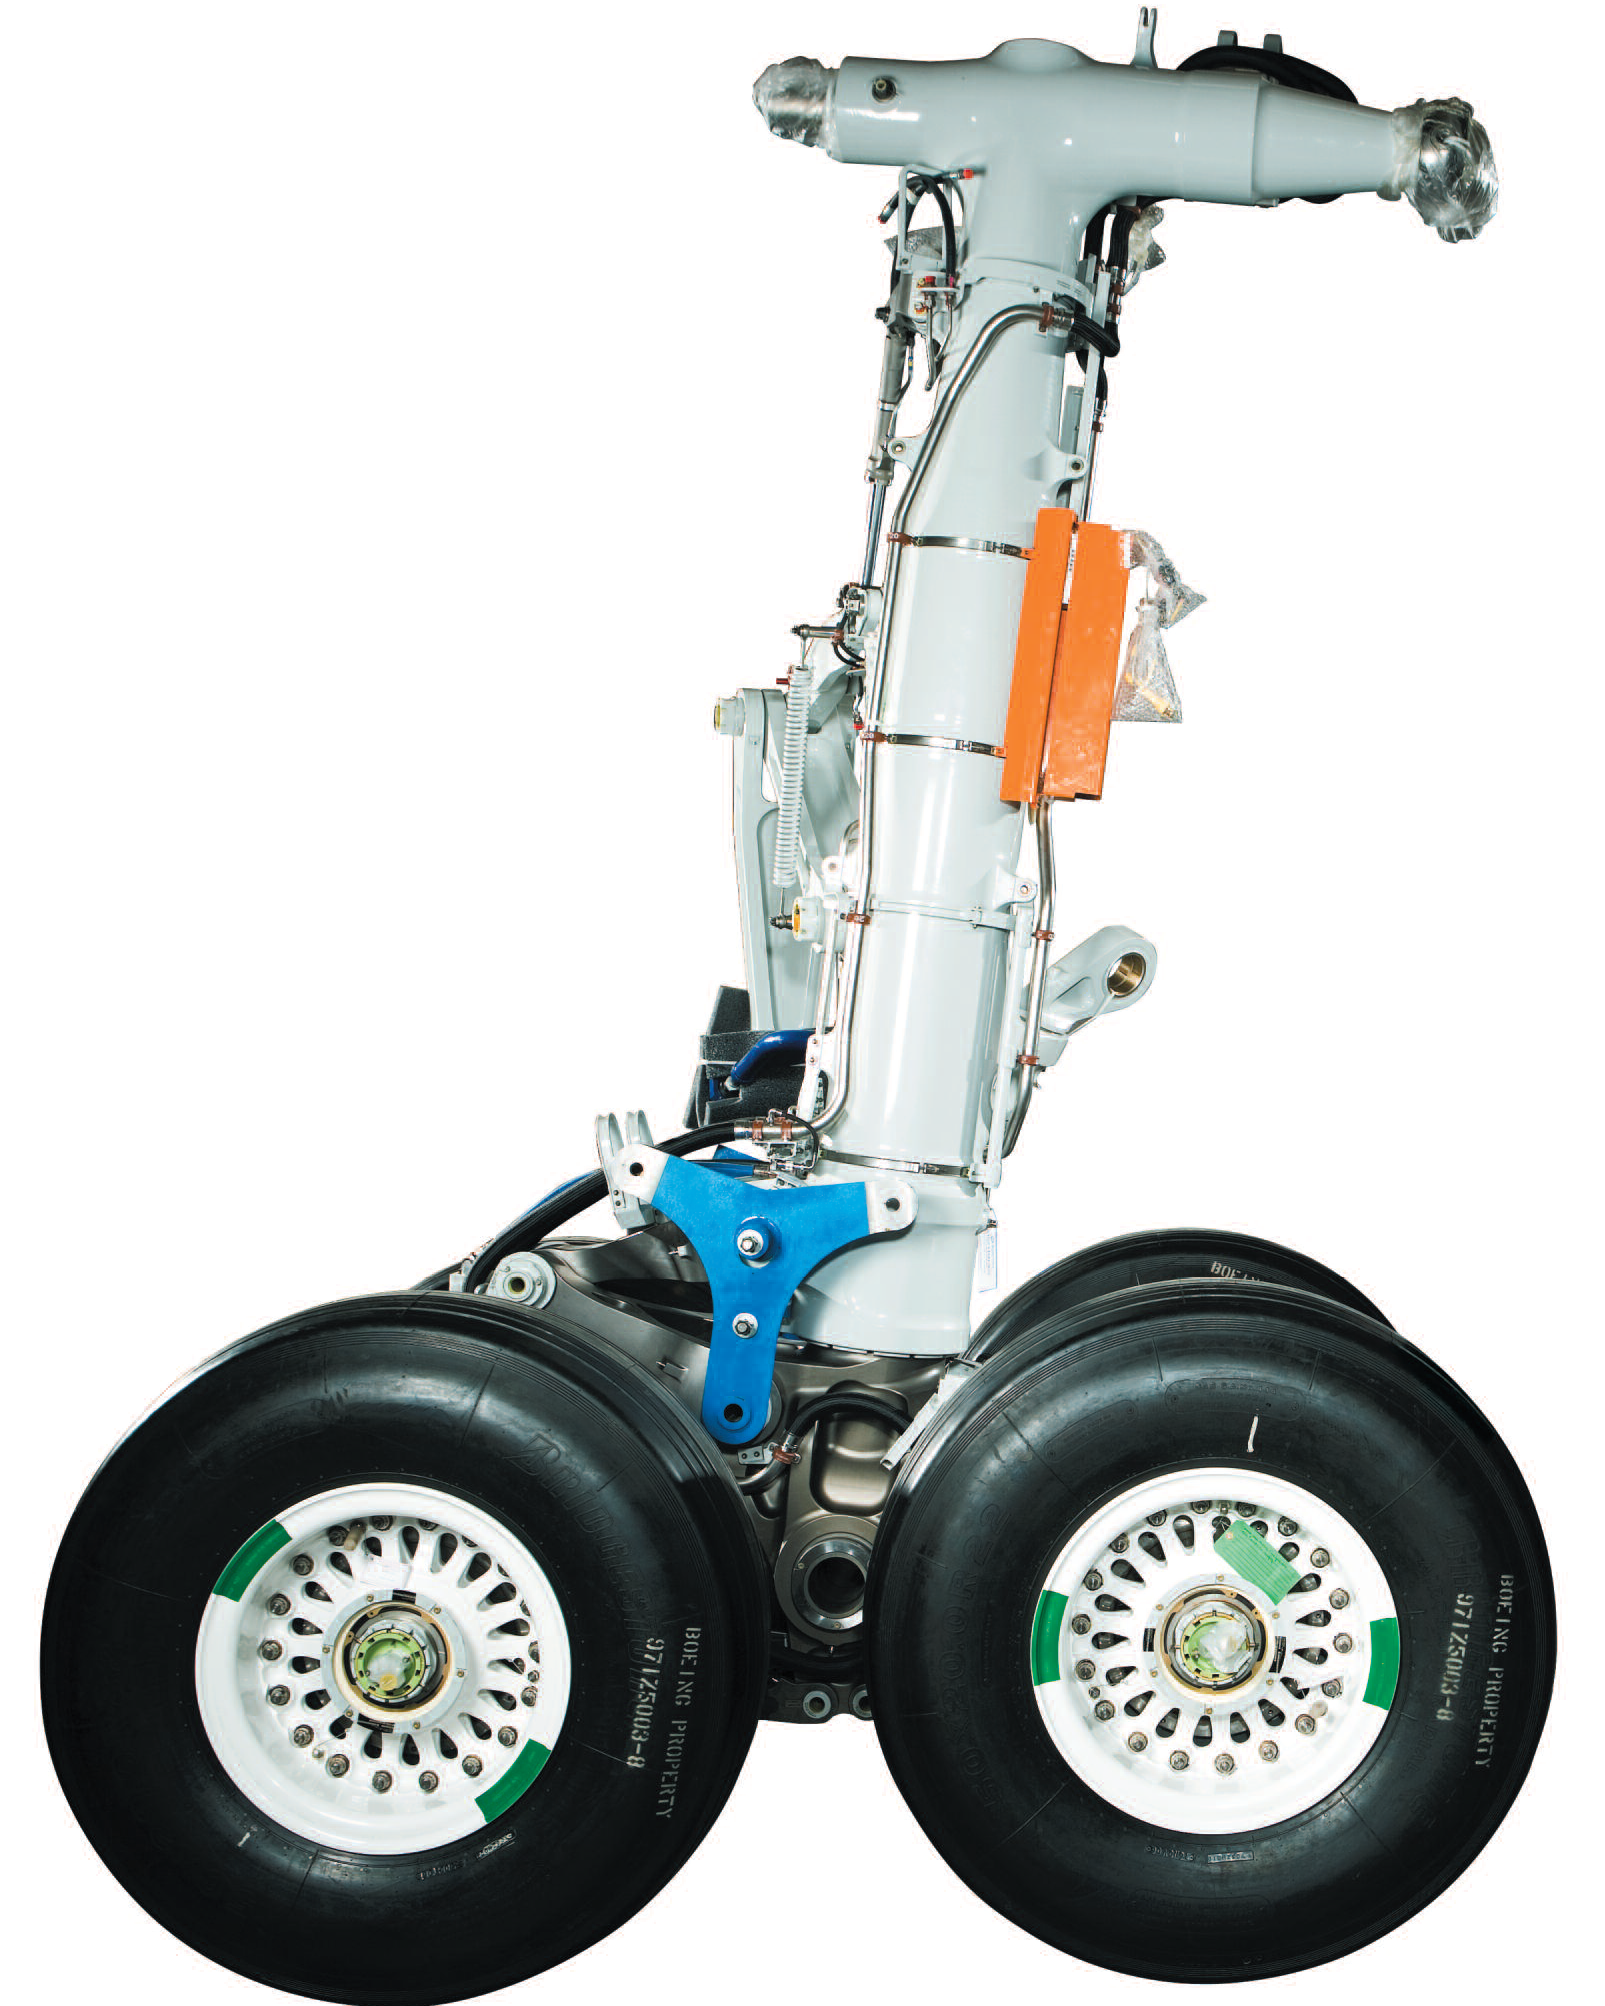
\includegraphics[width=\linewidth]{Images-2-EstudoConceitual/oleo_pneumatic.png} 
        \caption{Amortecedor óleo-pneumático \cite{globalspec_oleo}.}
        \label{fig:oleopneumatic}
    \end{minipage}
    \hfill
    % Segunda figura - Trailing Link
    \begin{minipage}{0.3\textwidth}
        \centering
        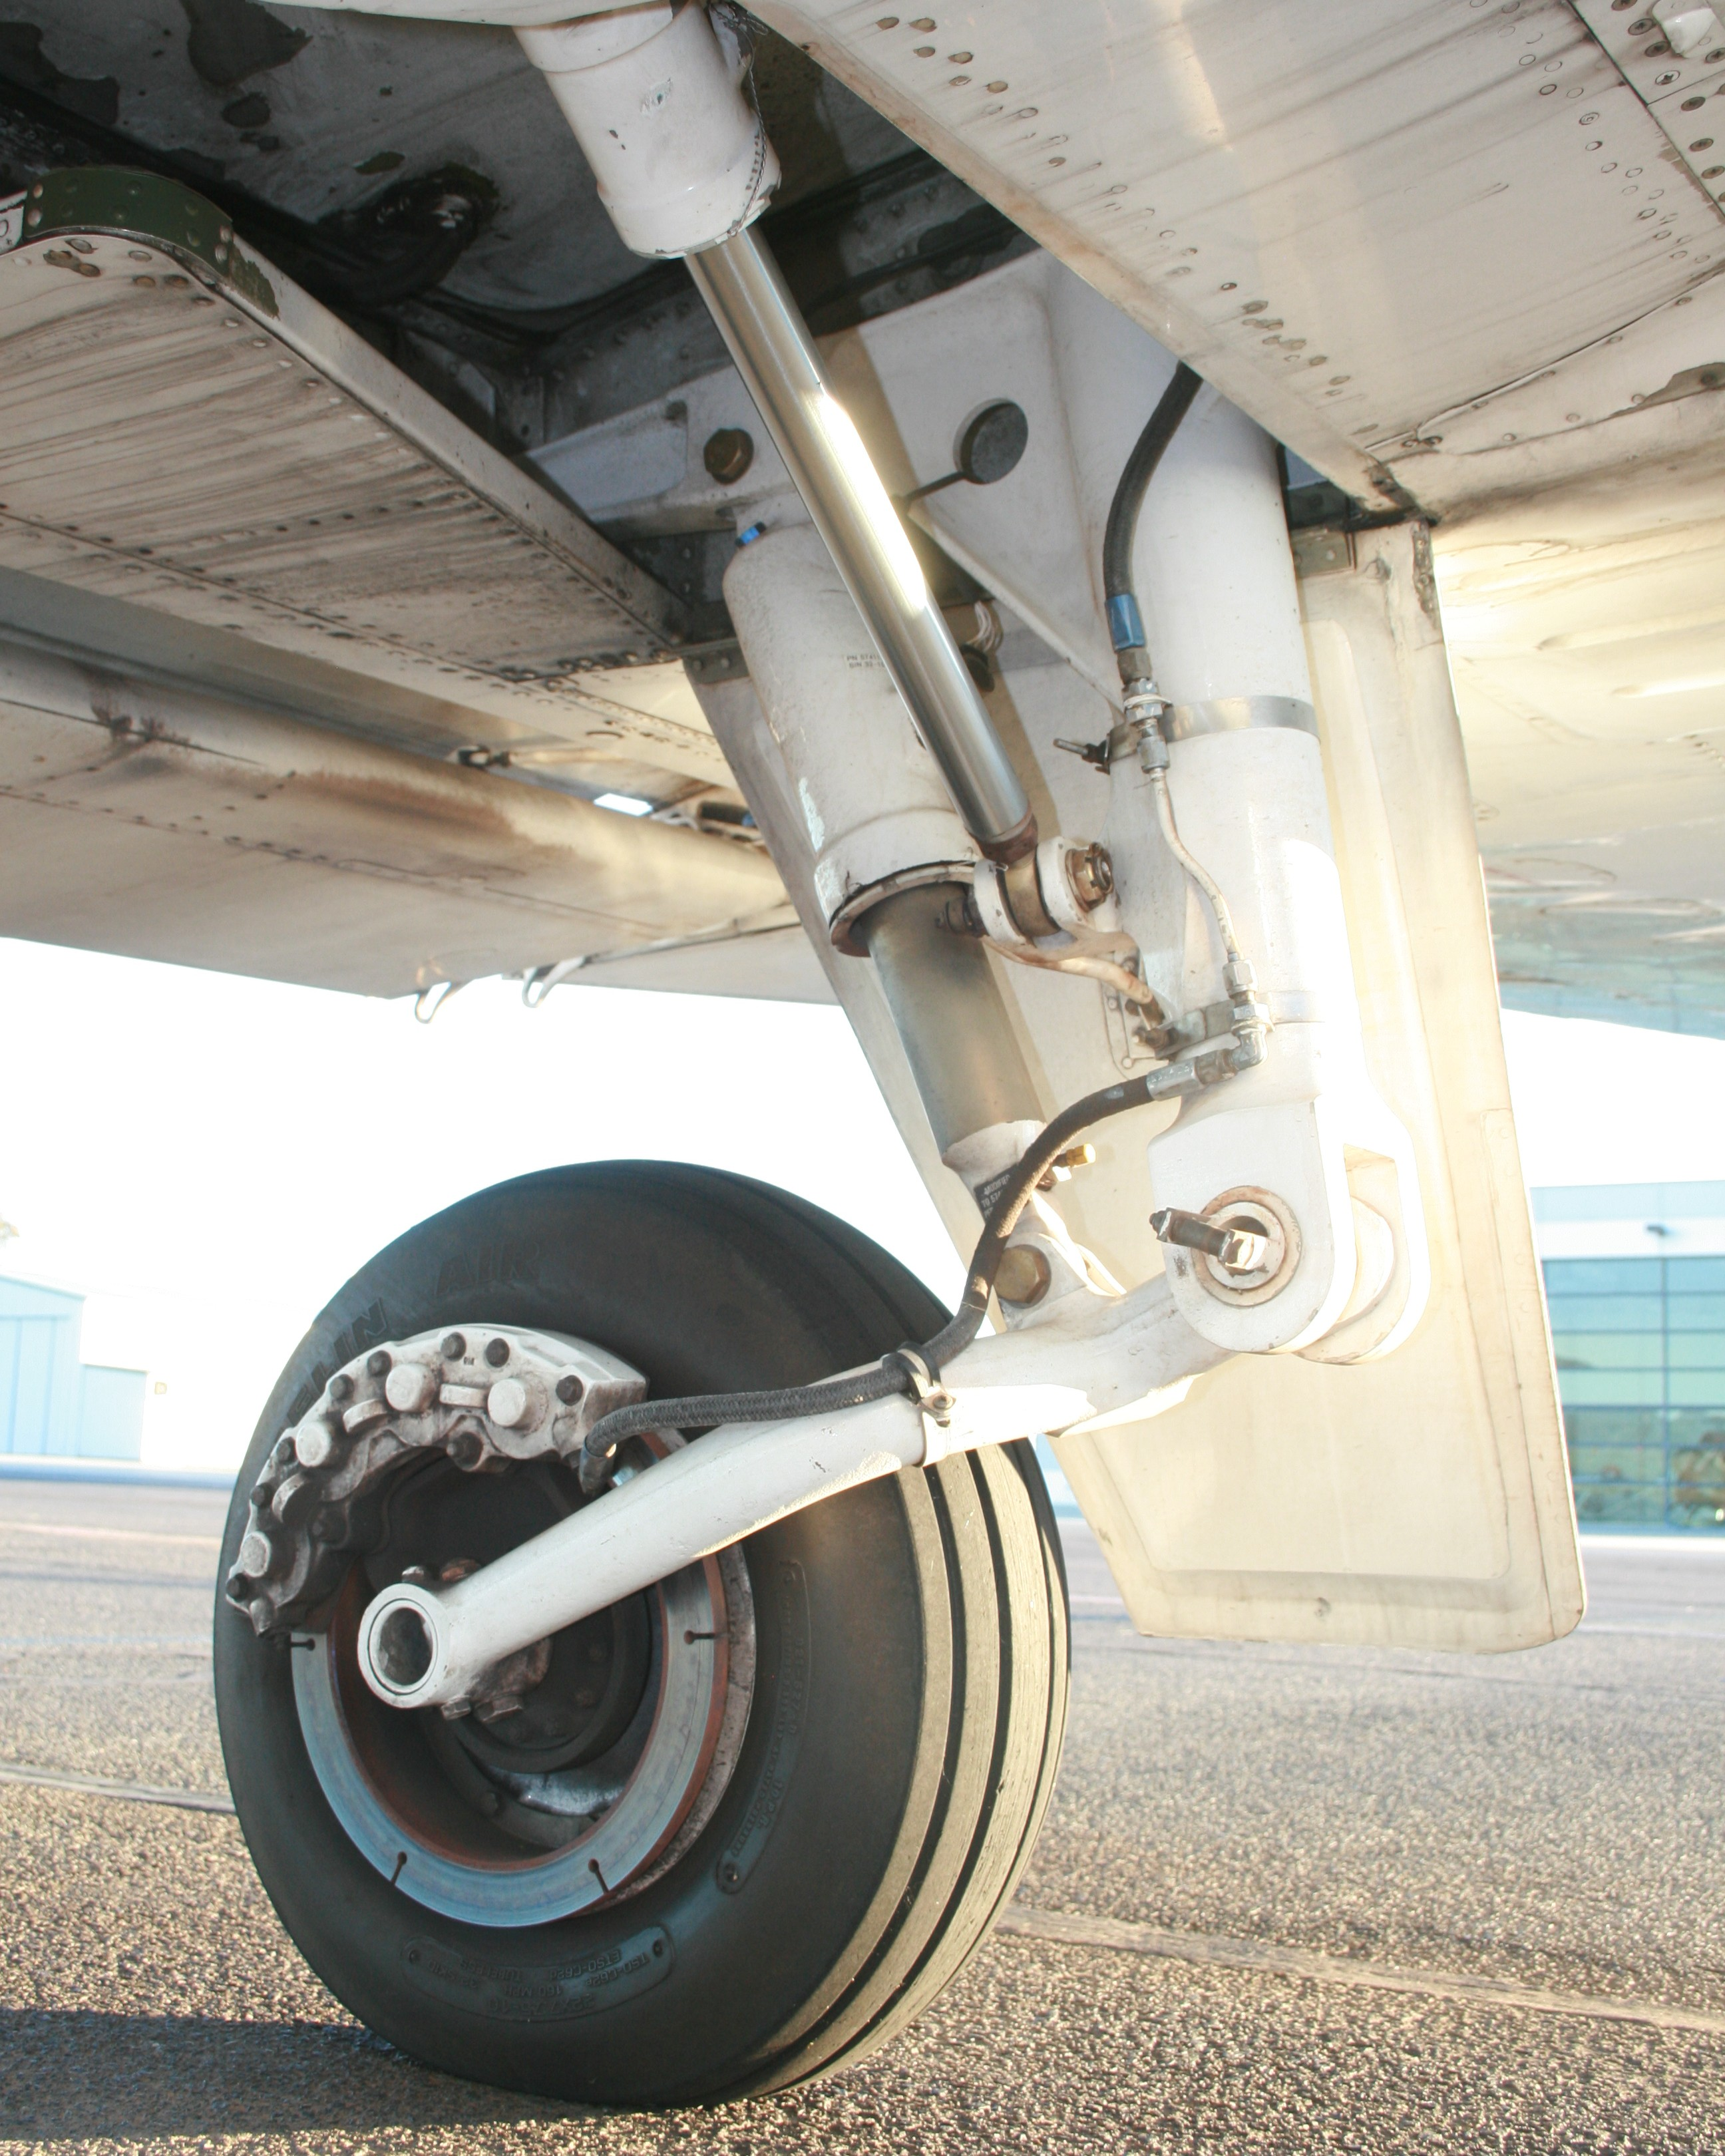
\includegraphics[width=\linewidth]{Images-2-EstudoConceitual/trailing_link.jpg} 
        \caption{Arquitetura de trem de pouso do tipo \textit{Trailing Link}\cite{wikimedia_trailing}.}
        \label{fig:TrailingArm}
    \end{minipage}
\end{figure}

Quanto ao funcionamento de amortecedores de trens de pouso óleo-pneumáticos, existem duas soluções principais: amortecedores com placa e metering pin ou com metering tube. O primeiro tipo, ilustrado na Figura \ref{fig:meteringpin}, se destaca por utilizar placas com orifício atravessadas por um pino de seção variável em um formato cônico, de forma que, quanto maior for a contração do trem de pouso após o contato completo com o solo, menor será a folga entre o orifício e o metering pin, aumentando a fricção do fluido com a estrutura e, consequentemente, dispersando a energia absorvida na forma de calor. Já os sistemas com metering tube, referenciados na Figura \ref{fig:meteringtube}, utilizam um tubo vazado com diversos orifícios, através dos quais o fluido é forçado durante a contração do trem, com o mesmo objetivo de rejeição de energia na forma de calor, sendo uma solução mais simplificada. 

Assim, para este projeto, a solução adotada será a do sistema com metering pin, uma vez que este é o sistema mais comumente usado, além de possuir a vantagem de permitir um ajuste e controle da dissipação de energia mais refinado quando comparado aos amortecedores com metering tube.

\begin{figure}[H]
    \centering
    % Primeira figura - metering pin
    \begin{minipage}{0.5\textwidth}
        \centering
        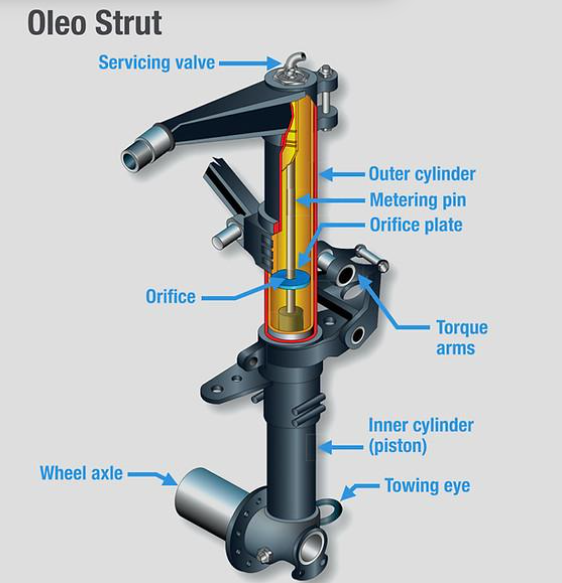
\includegraphics[width=\linewidth]{images/metering pin.png} 
        \caption{Amortecedor com metering pin \cite{meteringpin}.}
        \label{fig:meteringpin}
    \end{minipage}
    \hfill
    % Segunda figura - metering tube
    \begin{minipage}{0.3\textwidth}
        \centering
        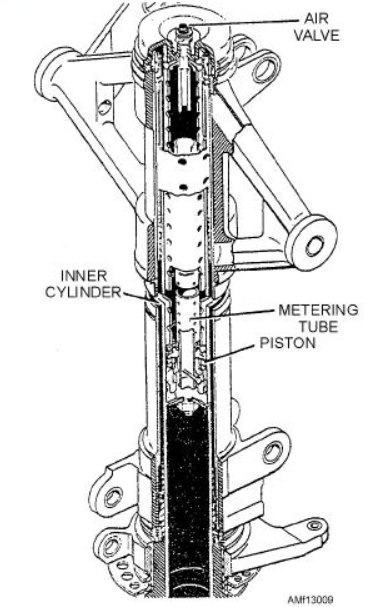
\includegraphics[width=\linewidth]{images/metering tube.png} 
        \caption{Amortecedor com metering tube \cite{meteringtube}.}
        \label{fig:meteringtube}
    \end{minipage}
\end{figure}


\section{Verificação de Requisitos e Tendências de Mercado}

Antes de consolidar as características gerais do protótipo e iniciar o projeto conceitual, é imprescindível confrontar os requisitos de missão estipulados com os dados reais de desempenho e peso dos concorrentes selecionados. Essa correlação gráfica permite validar se as metas do projeto são fisicamente factíveis e identificar os desafios tecnológicos que deverão ser superados.

A Figura \ref{fig:teto_v_cruzeiro} correlaciona o Teto de Operação com a Velocidade de Cruzeiro ($V_{cruise}$). O requisito do projeto exige uma operação a 260 kt e teto de 25.000 ft. Nota-se que o requisito encontra-se perfeitamente centralizado no envelope operacional da classe. Aeronaves como o BAe ATP e o ATR 72-600 operam com velocidades levemente superiores, enquanto o CASA C-295 apresenta um teto de serviço substancialmente maior (30.000 ft) devido à sua vocação tática. O ponto de projeto estipulado é, portanto, conservador e perfeitamente atingível com a tecnologia turboélice atual.

\begin{figure}[H]
    \centering
    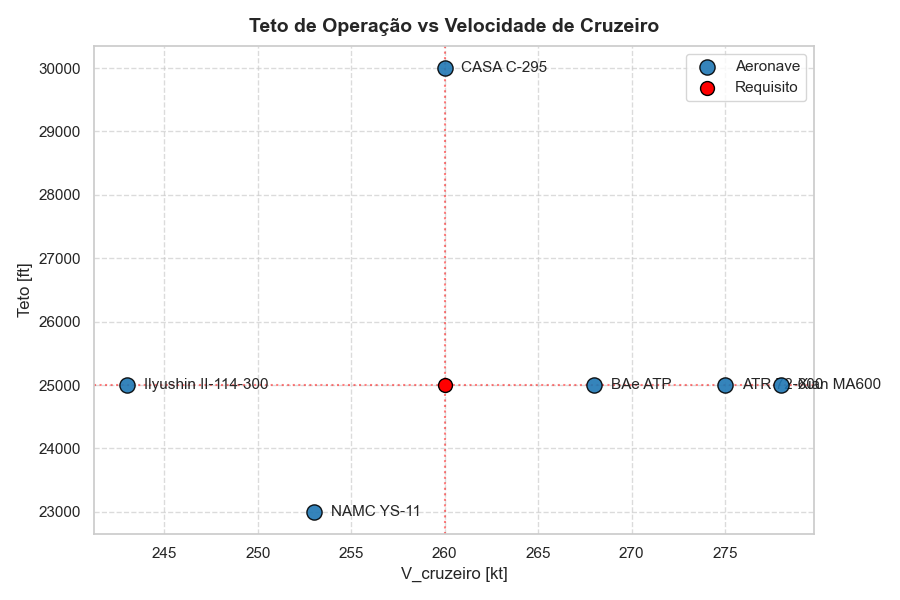
\includegraphics[width=0.7\linewidth]{Images-2-EstudoConceitual/teto_x_v_cruzeiro.png}
    \caption{Correlação entre Teto de Operação e Velocidade de Cruzeiro das aeronaves de referência em relação ao requisito de projeto.}
    \label{fig:teto_v_cruzeiro}
\end{figure}

Do ponto de vista de estimativa de massas, a Figura \ref{fig:pv_mtow} ilustra a relação entre o Peso Vazio (PV) e o Peso Máximo de Decolagem (MTOW). Observa-se uma tendência linear de crescimento do peso vazio em função do MTOW, característica típica demonstrada pelas formulações empíricas de Raymer \cite{raymer2018} e Roskam. O MTOW alvo do projeto encontra-se na faixa de 22.500 kgf. A dispersão dos dados mostra que aeronaves otimizadas para passageiros (como o ATR 72-600) conseguem manter um peso vazio estrutural mais baixo em relação ao MTOW do que aeronaves mais antigas ou adaptadas (como o YS-11), indicando a importância do uso de materiais compostos e ligas avançadas para o Projeto Conceitual.

\begin{figure}[H]
    \centering
    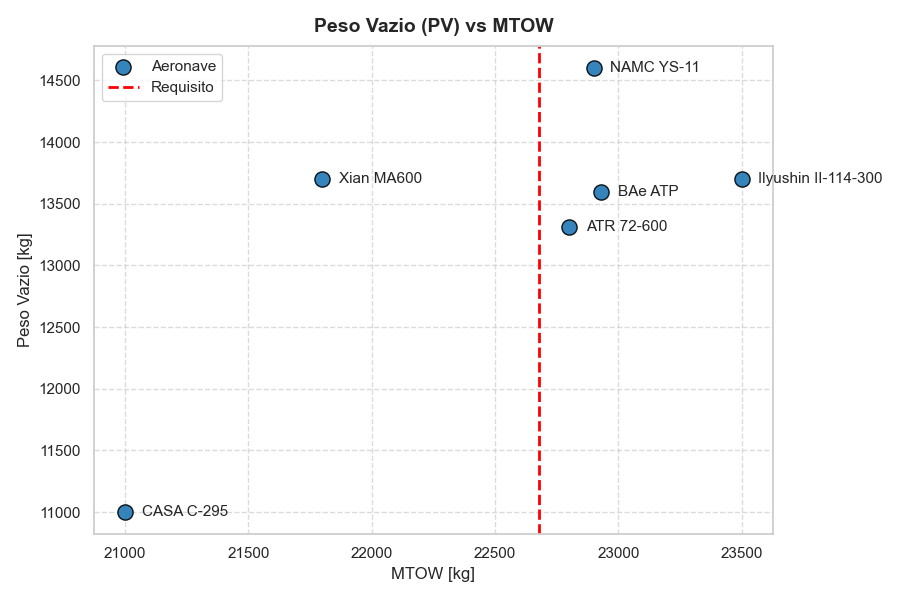
\includegraphics[width=0.7\linewidth]{Images-2-EstudoConceitual/pv_x_mtow.png}
    \caption{Tendência de Peso Vazio em função do Peso Máximo de Decolagem (MTOW).}
    \label{fig:pv_mtow}
\end{figure}

Por fim, o desempenho em pista é avaliado nas Figuras \ref{fig:pouso_mtow} e \ref{fig:decolagem_mtow}. O requisito de projeto dita um comprimento máximo de pista de aproximadamente 1.280 m para ambas as operações. 

\begin{figure}[H]
    \centering
    \begin{minipage}{0.48\textwidth}
        \centering
        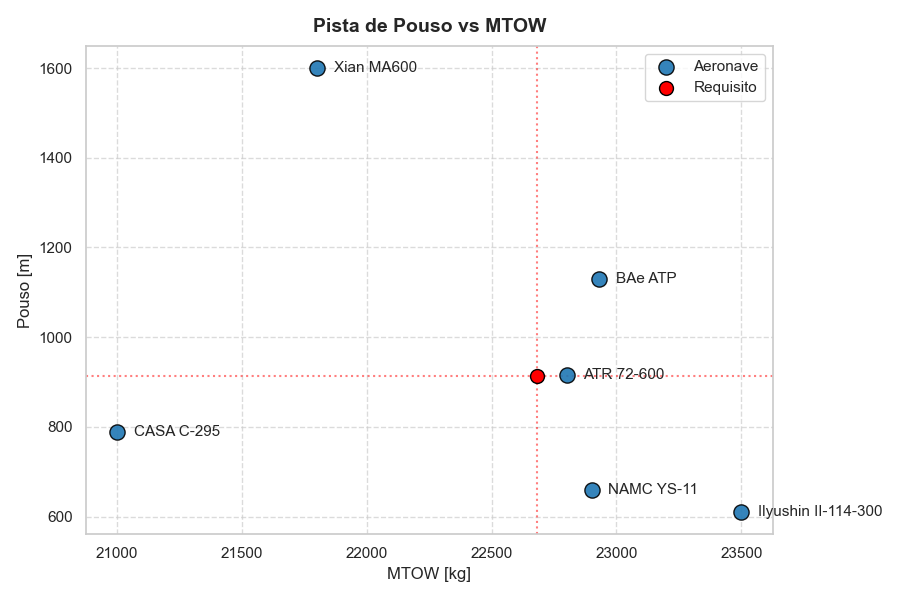
\includegraphics[width=\linewidth]{Images-2-EstudoConceitual/pouso_x_MTOW.png}
        \caption{Distância de Pouso vs MTOW.}
        \label{fig:pouso_mtow}
    \end{minipage}
    \hfill
    \begin{minipage}{0.48\textwidth}
        \centering
        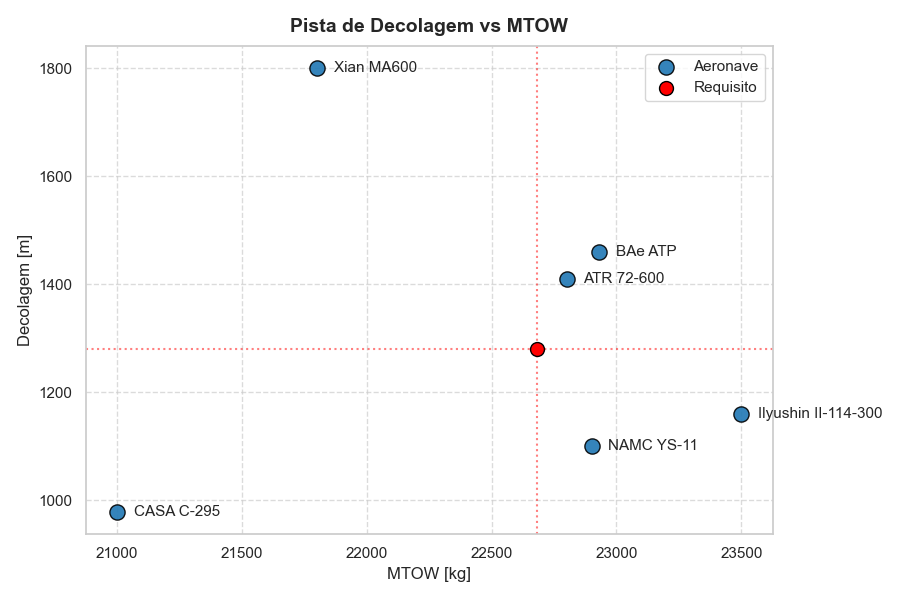
\includegraphics[width=\linewidth]{Images-2-EstudoConceitual/decolagem_x_mtow.png}
        \caption{Distância de Decolagem vs MTOW.}
        \label{fig:decolagem_mtow}
    \end{minipage}
\end{figure}

Para o pouso (Figura \ref{fig:pouso_mtow}), o requisito é atendido com certa margem pela maioria das aeronaves. No entanto, a decolagem (Figura \ref{fig:decolagem_mtow}) revela-se como a fase crítica limitante do projeto. Modelos como o ATR 72-600, Xian MA600 e BAe ATP ultrapassam a restrição de decolagem, evidenciando que, para atingir o MTOW de projeto e ainda operar em pistas curtas, o Projeto Conceitual precisará focar rigorosamente em um sistema hipersustentador eficiente (elevado $C_{L_{max}}$ de decolagem) e em uma baixa carga alar ($W/S$).

\section{Delimitação Geral do Protótipo}

Após a análise comparativa detalhada e a avaliação das características predominantes entre os competidores diretos, a Tabela \ref{tab:delimitacao_prototipo} sintetiza as configurações selecionadas para o desenvolvimento do Projeto Conceitual da aeronave.

\begin{table}[h!]
\centering
\caption{Características desejadas para os componentes da aeronave.}
\label{tab:delimitacao_prototipo}
\vspace{0.2cm} % Espaço leve entre o caption e a tabela
\renewcommand{\arraystretch}{1.2} % Aumenta um pouco o espaçamento vertical das linhas para ficar mais parecido com a imagem
\begin{tabular}{lcc}
\hline
\textbf{Componente} & \textbf{Características desejadas} & \\
\hline
\multirow{2}{*}{Asa} & Configuração & Asa alta \\
 & Forma em planta & Trapezoidal \\
\hline
\multirow{3}{*}{Cauda} & Configuração das empenagens & Baixa \\
 & Forma em planta horizontal & Trapezoidal \\
 & Forma em planta vertical & Trapezoidal \\
\hline
\multirow{2}{*}{Motorização} & Número de motores & 2 \\
 & Tipo de motor & Turboélice \\
\hline
\multirow{2}{*}{Trem de pouso} & Configuração & Triciclo \\
 & Tipo & Retrátil \\
\hline
\end{tabular}
\end{table}



\chapter{Projeto Conceitual}
\section{Geometria Interna}
Com base nos parâmetros levantados na seção anterior e em requisitos normativos aplicáveis, procedeu-se ao dimensionamento detalhado da geometria interna da cabine. Conforme observa Raymer (1992), o arranjo interno de uma aeronave é ditado mais por decisões de mercado do que por regulamentações, fato que se reflete diretamente na padronização de pitch, largura do assento e largura do corredor observada entre as aeronaves previamente estudadas.

Nesse contexto, a configuração aqui apresentada corresponde à configuração comercial para transporte de passageiros, identificada pelo estudo de mercado como a operação predominante ao longo da vida útil de aeronaves similares. A configuração cargueiro, que utiliza os mesmos trilhos estruturais para receber Unit Load Devices (ULDs), contêineres e pallets padronizados, será abordada em seção posterior.

Conforme discutido anteriormente, a cabine adotará uma configuração de 4 assentos por fileira, separados por um corredor central - padrão dominante na classe de turboélices regionais desse porte. Para escolha das dimensões internas, utilizou-se como referência principal a Tabela 9.1 de Raymer (1992), que fornece valores típicos de pitch, largura de assento, largura e altura de corredor, e volume de galley para as categorias de primeira classe, econômica e alta densidade.

A aeronave projetada enquadra-se predominantemente na categoria econômica, com elementos da coluna de alta densidade em função da faixa de capacidade especificada na descrição da missão (60 a 70 PAX) e do caráter regional de curto e médio alcance da missão.

O comprimento da cabine foi definido em 16.00 m, correspondente à média dos valores observados em aeronaves do estudo comparativo. Além disso, esse valor se mostrou adequado para acomodar a capacidade proposta de passageiros e está próximo ao da aeronave de referência mais similar - o ATR-72 (17.00 m). A largura da cabine foi definida em 2.6 m, valor também coerente com aeronaves similares e adequado para comportar os assentos e o espaço de corredor desejado. O layout em planta resultante é apresentado na Figura~\ref{fig:layout_planta}.

\begin{figure}[H]
\centering
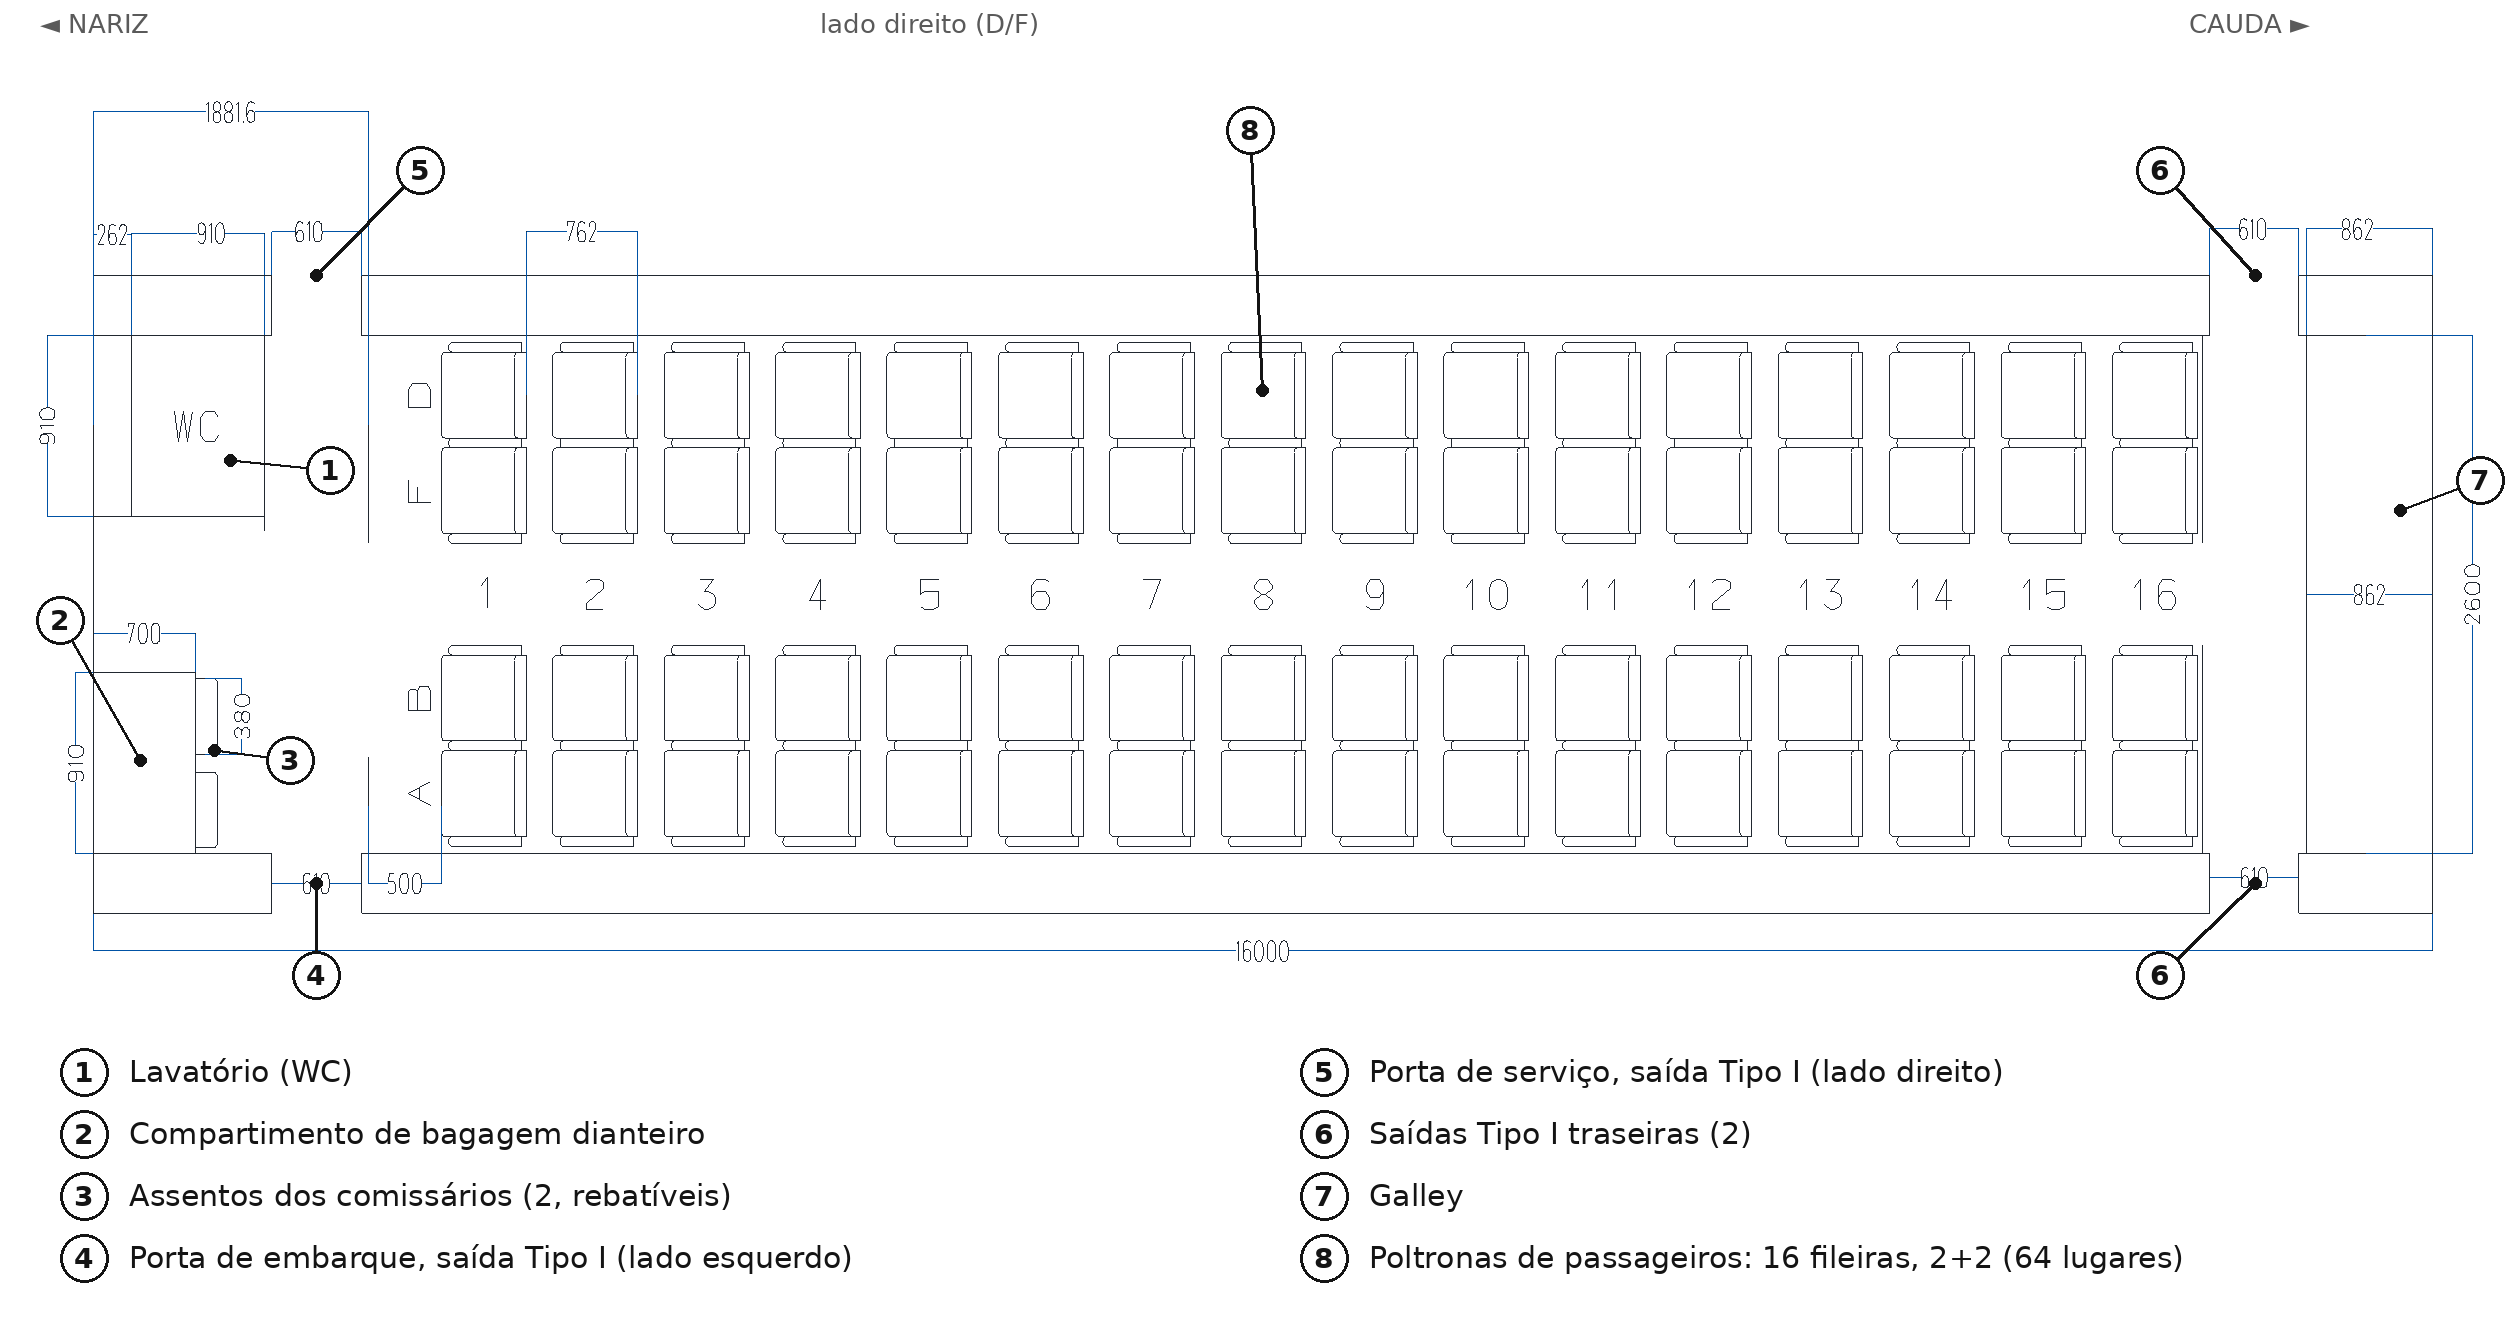
\includegraphics[width=\textwidth]{images/cabine_planta.png}
\caption{Layout em planta da cabine de passageiros, com indicação dos assentos dos comissários, saídas, lavatório, galley e compartimento de bagagem. Dimensões em milímetros.}
\label{fig:layout_cabine}
\end{figure}

Conforme mostra a figura, a cabine comporta 16 fileiras numeradas de 1 a 16, com identificação pelas letras A/B (esquerda) e D/F (direita). O pitch adotado é 762 mm (30 in), enquadrando-se na faixa de 30 a 32 in da categoria de alta densidade indicada por Raymer (1992). Nas extremidades da cabine, a zona de serviço dianteira ocupa 1881.6 mm de comprimento, acomodando um lavatório, dois compartimentos para pequenas bagagens, duas saídas de emergência (incluindo a porta de embarque) e dois assentos para tripulação. O lavatório foi posicionado na zona dianteira de modo a facilitar o acesso pela tripulação quando aplicada a configuração de carga. A zona de serviço traseira compreende 1625.5 mm de comprimento, compreendendo a galley e duas saídas de emergência. A capacidade total resultante é de 64 passageiros.

No que se refere às saídas de emergência, o RBAC 25.807 exige que todos os ocupantes possam evacuar a aeronave em até 90 segundos. Então, o layout prevê quatro saídas de emergência Tipo I posicionadas nas zonas dianteira e traseira (largura mínima de 610~mm, altura mínima de 1220~mm). Essa combinação de saídas atende plenamente ao requisito normativo de capacidade de evacuação e está coerente com as aeronaves analisadas, garantindo fluxo suficiente mesmo na condição de máxima ocupação prevista.

Ainda com base no comparativo previamente apresentado, também foi feito o dimensionamento detalhado da seção transversal, apresentada na Figura~\ref{fig:secao_transversal}.

\begin{figure}[H]
    \centering
    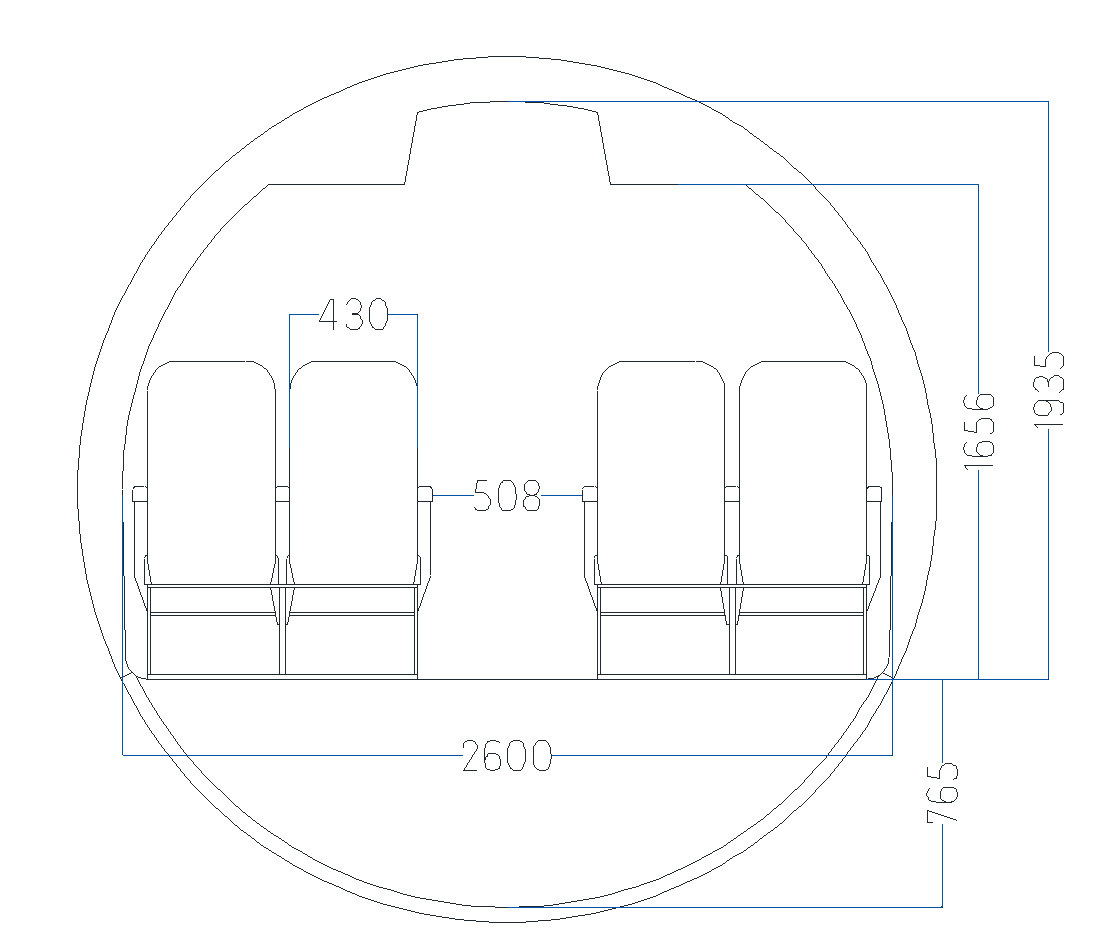
\includegraphics[width=0.65\linewidth]{images/secao_transversal.png}
    \caption{Seção transversal da cabine com configuração 2+2. Dimensões em milímetros.}
    \label{fig:secao_transversal}
\end{figure}

Cada assento possui 430 mm (16.9 in) de largura, valor compatível com a faixa de 16 - 22 in proposta por Raymer (1992) para as categorias econômica e alta densidade. O corredor central foi dimensionado em 508 mm (20 in), também enquadrando-se na faixa proposta e superando os limites mínimos de 381 mm ao nível do ombro e 406 mm ao nível do quadril estabelecidos pelo \S 25.815 do 14 CFR Part 25. As dimensões de encosto de braço e suportes dos bancos foram estimadas com base em imagens de aeronaves similares.

A altura livre interna, medida do piso até o teto sobre o corredor, é de 1935 mm (76.2 in), consistente com aeronaves similares e com o limite mínimo de 76 in indicado por Raymer (1992) para as categorias econômica e primeira classe, e consistente
com as aeronaves do comparativo. A altura entre o piso e compartimento superior (overhead bin) é de 1656 mm (65.2 in), também compatível com a categoria de primeira classe e econômica. A cota de 765 mm entre o piso e a base da estrutura engloba o assoalho estrutural, os trilhos de fixação de assentos e a câmara inferior destinada ao porão de carga.

Complementando a versatilidade operacional da aeronave, projetou-se uma configuração de carga do tipo \textit{Quick Change} (QC), que permite a conversão da cabine de passageiros para cargueiro em tempo reduzido. Esta flexibilidade é fundamental para a operação regional, permitindo que a aeronave atenda ao transporte de passageiros em horários de pico e atue como cargueiro puro em períodos de baixa demanda ou voos noturnos.


Para a operação cargueira, selecionou-se o palete padronizado IATA PLA (Half Pallet), com dimensões de base de $1534 \times 3175$ mm, conforme a figura \ref{fig:palete} em anexo. A escolha deste dispositivo justifica-se pela total compatibilidade com a infraestrutura logística global, facilitando a intermodalidade. 


Embora a cabine possua um diâmetro interno de 2,6 m, o uso do palete PLA permite a manutenção de um corredor funcional para inspeção ou folga estrutural de $0{,}53$~m. Diferente de contêineres rígidos, o palete com rede oferece a flexibilidade necessária para adaptar o contorno da carga (\textit{contouring}) à curvatura da fuselagem da aeronave, otimizando o volume disponível sem comprometer a integridade dos painéis internos e revestimentos. Nas figuras \ref{fig:palete_frontal} e \ref{fig:palete_superior} pode-se observar a disposição dos paletes no \textit{Main Deck} em uma vista superior e frontal através das figuras hachuradas,  bem como uma destinação no final da aeronave para bagagens, vale ressaltar que o \textit{Lower Deck} também será destinado para bagagens.


\begin{figure}[H]
    \centering
    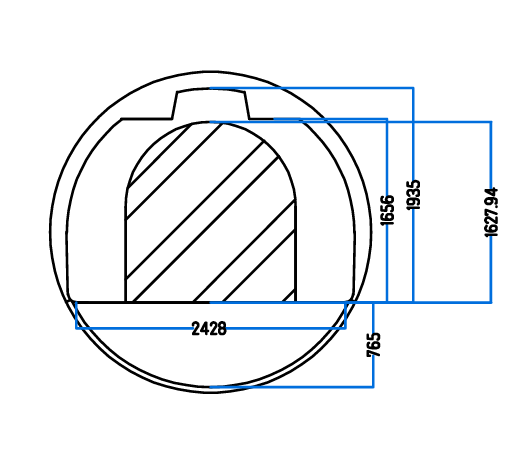
\includegraphics[width=0.4\linewidth]{images/palete_frontal.png}
    \caption{Vista Frontal}
    \label{fig:palete_frontal}
\end{figure}

\begin{figure}[H]
    \centering
    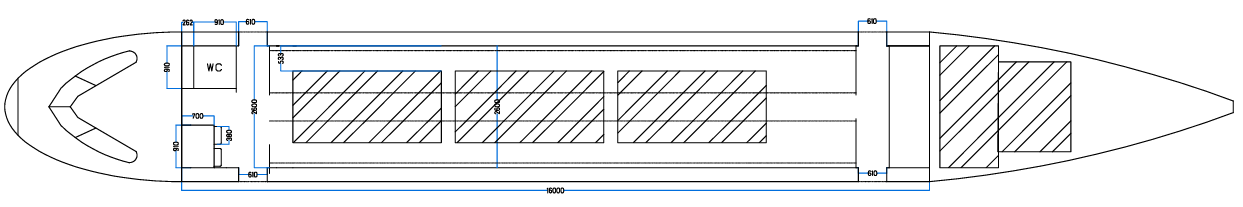
\includegraphics[width=1\linewidth]{images/palete_superior.png}
    \caption{Vista Superior}
    \label{fig:palete_superior}
\end{figure}

A transição rápida entre as configurações é viabilizada pela utilização dos trilhos estruturais mencionados na seção anterior. O piso da aeronave é equipado com trilhos universais de alta resistência, operando da seguinte forma:

\begin{itemize}
    \item \textbf{Configuração de Passageiros:} Os assentos são montados sobre "paletes de assento" (seat pallets) que se travam diretamente nos trilhos. Isso permite que as fileiras sejam removidas em blocos, minimizando o tempo de solo (\textit{turnaround}).
    \item \textbf{Configuração de Carga:} Após a remoção dos assentos, os mesmos trilhos recebem os \textit{locks} (travas) mecânicos para fixação dos paletes PLA. Para a movimentação interna, o piso integra esferas e roletes escamoteáveis (\textit{omni-directional rollers}), que permitem o deslize manual de cargas de até 3175 kg com esforço reduzido da equipe de solo.
\end{itemize}


\section{Geometria da Asa}

A fim de validar as escolhas de projeto abordadas teoricamente, realizou-se um levantamento estatístico restrito aos seis concorrentes diretos previamente selecionados (ATR 72-600, CASA C-295, Il-114-300, BAe ATP, NAMC YS-11 e Xian MA600). A Figura \ref{fig:pie_posicao_asa} ilustra a distribuição de mercado referente à posição da asa dessas aeronaves.

\begin{figure}[H]
    \centering
    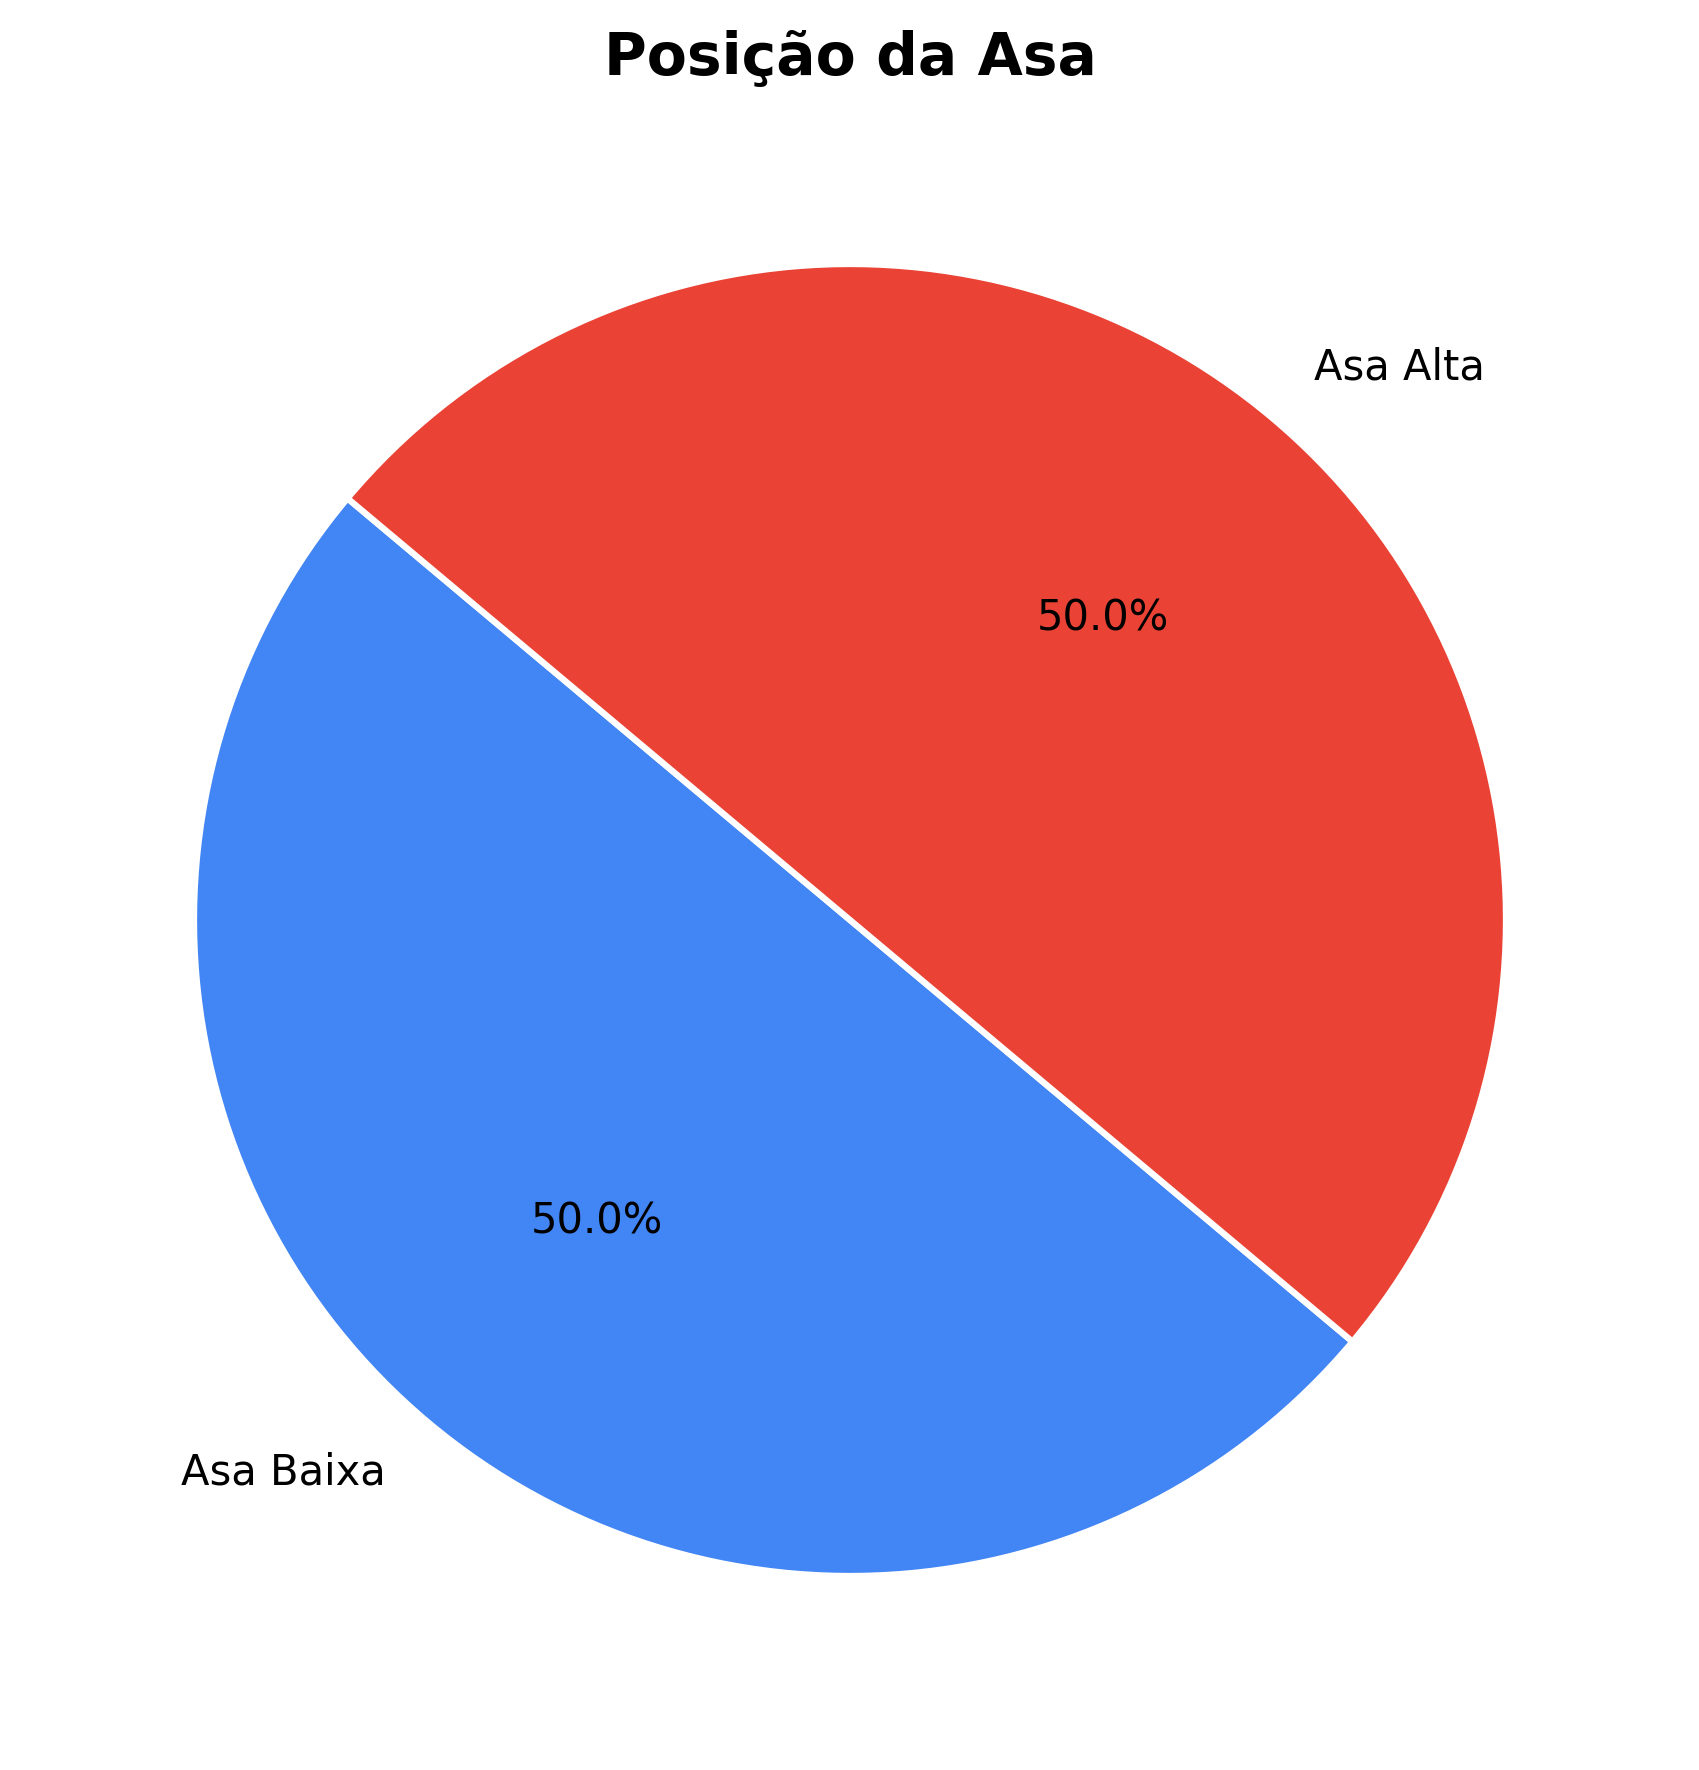
\includegraphics[width=0.4\linewidth]{Images-2-EstudoConceitual/pizza_asa.png} % Ajuste o caminho se necessário
    \caption{Distribuição da posição da asa entre os concorrentes diretos.}
    \label{fig:pie_posicao_asa}
\end{figure}

Conforme os dados apresentados, não há um consenso absoluto no mercado regional quanto à posição da asa, havendo um empate exato (50\% para cada) entre a adoção de asa alta e asa baixa. No entanto, corroborando a teoria de Anderson \cite{anderson1999}, a configuração de asa alta foi a selecionada para consolidar o Projeto Conceitual. Essa escolha alinha-se aos modelos de maior sucesso comercial e versatilidade (como o ATR 72 e o C-295), favorece o embarque de mercadorias em pistas com infraestrutura escassa e garante o distanciamento seguro das hélices de grande diâmetro em relação ao solo.

No que tange à geometria da planta, observa-se, dentre as aeronaves de referência, uma adoção única de formas trapezoidais entre o grupo de competidores avaliado. Essa unanimidade fundamenta-se no excelente compromisso aerodinâmico alcançado: a asa trapezoidal permite uma boa aproximação da distribuição de sustentação elíptica ideal (que minimiza drasticamente o arrasto induzido), ao mesmo tempo em que apresenta custos e complexidades de manufatura substancialmente menores quando comparada às asas elípticas ou compostas. Portanto, guiado pelas tendências das aeronaves de referência, este projeto adotará uma asa alta de geometria trapezoidal.

O ângulo de enflechamento definido foi zero, uma vez que seus principais benefícios estão associados a regimes transônicos e supersônicos, não sendo necessários para a faixa de velocidades prevista para a aeronave. Para o diedro, optou-se pela utilização de anedro, com \(\Gamma=-2,8^\circ\). Essa escolha está associada à configuração de asa alta adotada, que naturalmente apresenta um efeito estabilizante lateral pronunciado. A introdução de um anedro moderado permite reduzir esse efeito restaurador, proporcionando uma resposta mais adequada aos comandos de rolamento e evitando uma estabilidade lateral excessiva. O valor adotado constitui uma estimativa preliminar de projeto, devendo sua adequação ser posteriormente verificada nas análises de estabilidade látero-direcional da aeronave.

\begin{itemize}
    \item Raiz da Asa: NACA 43018
    \item Ponta da Asa: NACA 43013

\end{itemize}

Além disso, as dimensões das superfícies de comando da asa também foram baseadas nessa aeronave. Para envergadura, corda da raiz e corda da ponta, foi calculada a média entre os valores extremos para essas dimensões nas seis aeronaves semelhantes. Esse método permite utilizar de forma mais direta a amplitude do envelope de projeto praticado pelos concorrentes, garantindo que a aeronave seja competitiva dentro dos limites operacionais já validados pelo mercado. Os valores desses parâmetros são apresentados na tabela \ref{tab:dimensões da asa}.

\begin{table}[H]
  \centering
  \linespread{1}\small
  \setlength{\tabcolsep}{4pt}
  \caption{Parâmetros geométricos da asa e superfícies de controle.}
  \label{tab:dimensões da asa}
  \begin{tabularx}{\textwidth}{L C}
    \toprule
    \textbf{Dimensão} & \textbf{Valor} \\
    \midrule
    Envergadura (b) & 28,5 m \\
    Corda da raiz & 3,7 m \\
    Corda da ponta & 1,5 m \\
    Aileron & 3,8 m (comp.) / 0,92 m (larg.) \\
    Flap & 8,7 m (comp.) / 0,44 m (larg.) \\
    \bottomrule
  \end{tabularx}
\end{table}

Por fim, o afilamento, o alongamento, a área alar e a corda média aerodinâmica foram calculados pelas relações geométricas clássicas dadas pelas equações \eqref{área alar} a \eqref{corda média aerodinâmica}, usando os valores determinados no processo descrito anteriormente.

\begin{equation}
S = \frac{b \, (c_{raiz} + c_{ponta})}{2} = \frac{28,5 \cdot (3,7 + 1,5)}{2} = 74,1 \, m^2
\label{área alar}
\end{equation}

\begin{equation}
\lambda = \frac{c_{ponta}}{c_{raiz}} = \frac{1,5}{3,7} \approx 0,405
\label{afilamento}
\end{equation}

\begin{equation}
AR = \frac{b^2}{S} = \frac{28,5^2}{74,1} \approx 10,96
\label{alongamento}
\end{equation}

\begin{equation}
\bar{c} = \frac{2}{3} \, c_{raiz} \, \frac{1 + \lambda + \lambda^2}{1 + \lambda} = \frac{2}{3} \cdot 3,7 \cdot \frac{1 + 0,405 + 0,405^2}{1 + 0,405} \approx 2,75 \, m
\label{corda média aerodinâmica}
\end{equation}

%%%%%%%%%%%%%%%%%%%%%%%%%%%%%%%%%%%%%%%%%%%%%%%%%%%%%%%%%%%%%%%%%%%%%
%%%%%%%%%%%%%%%%%%%%%%%%%%%%%%%%%%%%%%%%%%%%%%%%%%%%%%%%%%%%%%%%%%%%%
%%%%%%%%%%%%%%%%%%%%%%%%%%%%%%%%%%%%%%%%%%%%%%%%%%%%%%%%%%%%%%%%%%%%%

\section{Geometria da Empenagem}
Para embasar a seleção da arquitetura de cauda, avalia-se a tendência adotada pelas aeronaves de referência concorrentes. A Figura \ref{fig:tipo_empenage} mostra que 83,3\% adotam empenagem convencional, sendo o ATR 72-600 a única exceção entre os concorrentes diretos.

\begin{figure}[htbp]
    \centering
    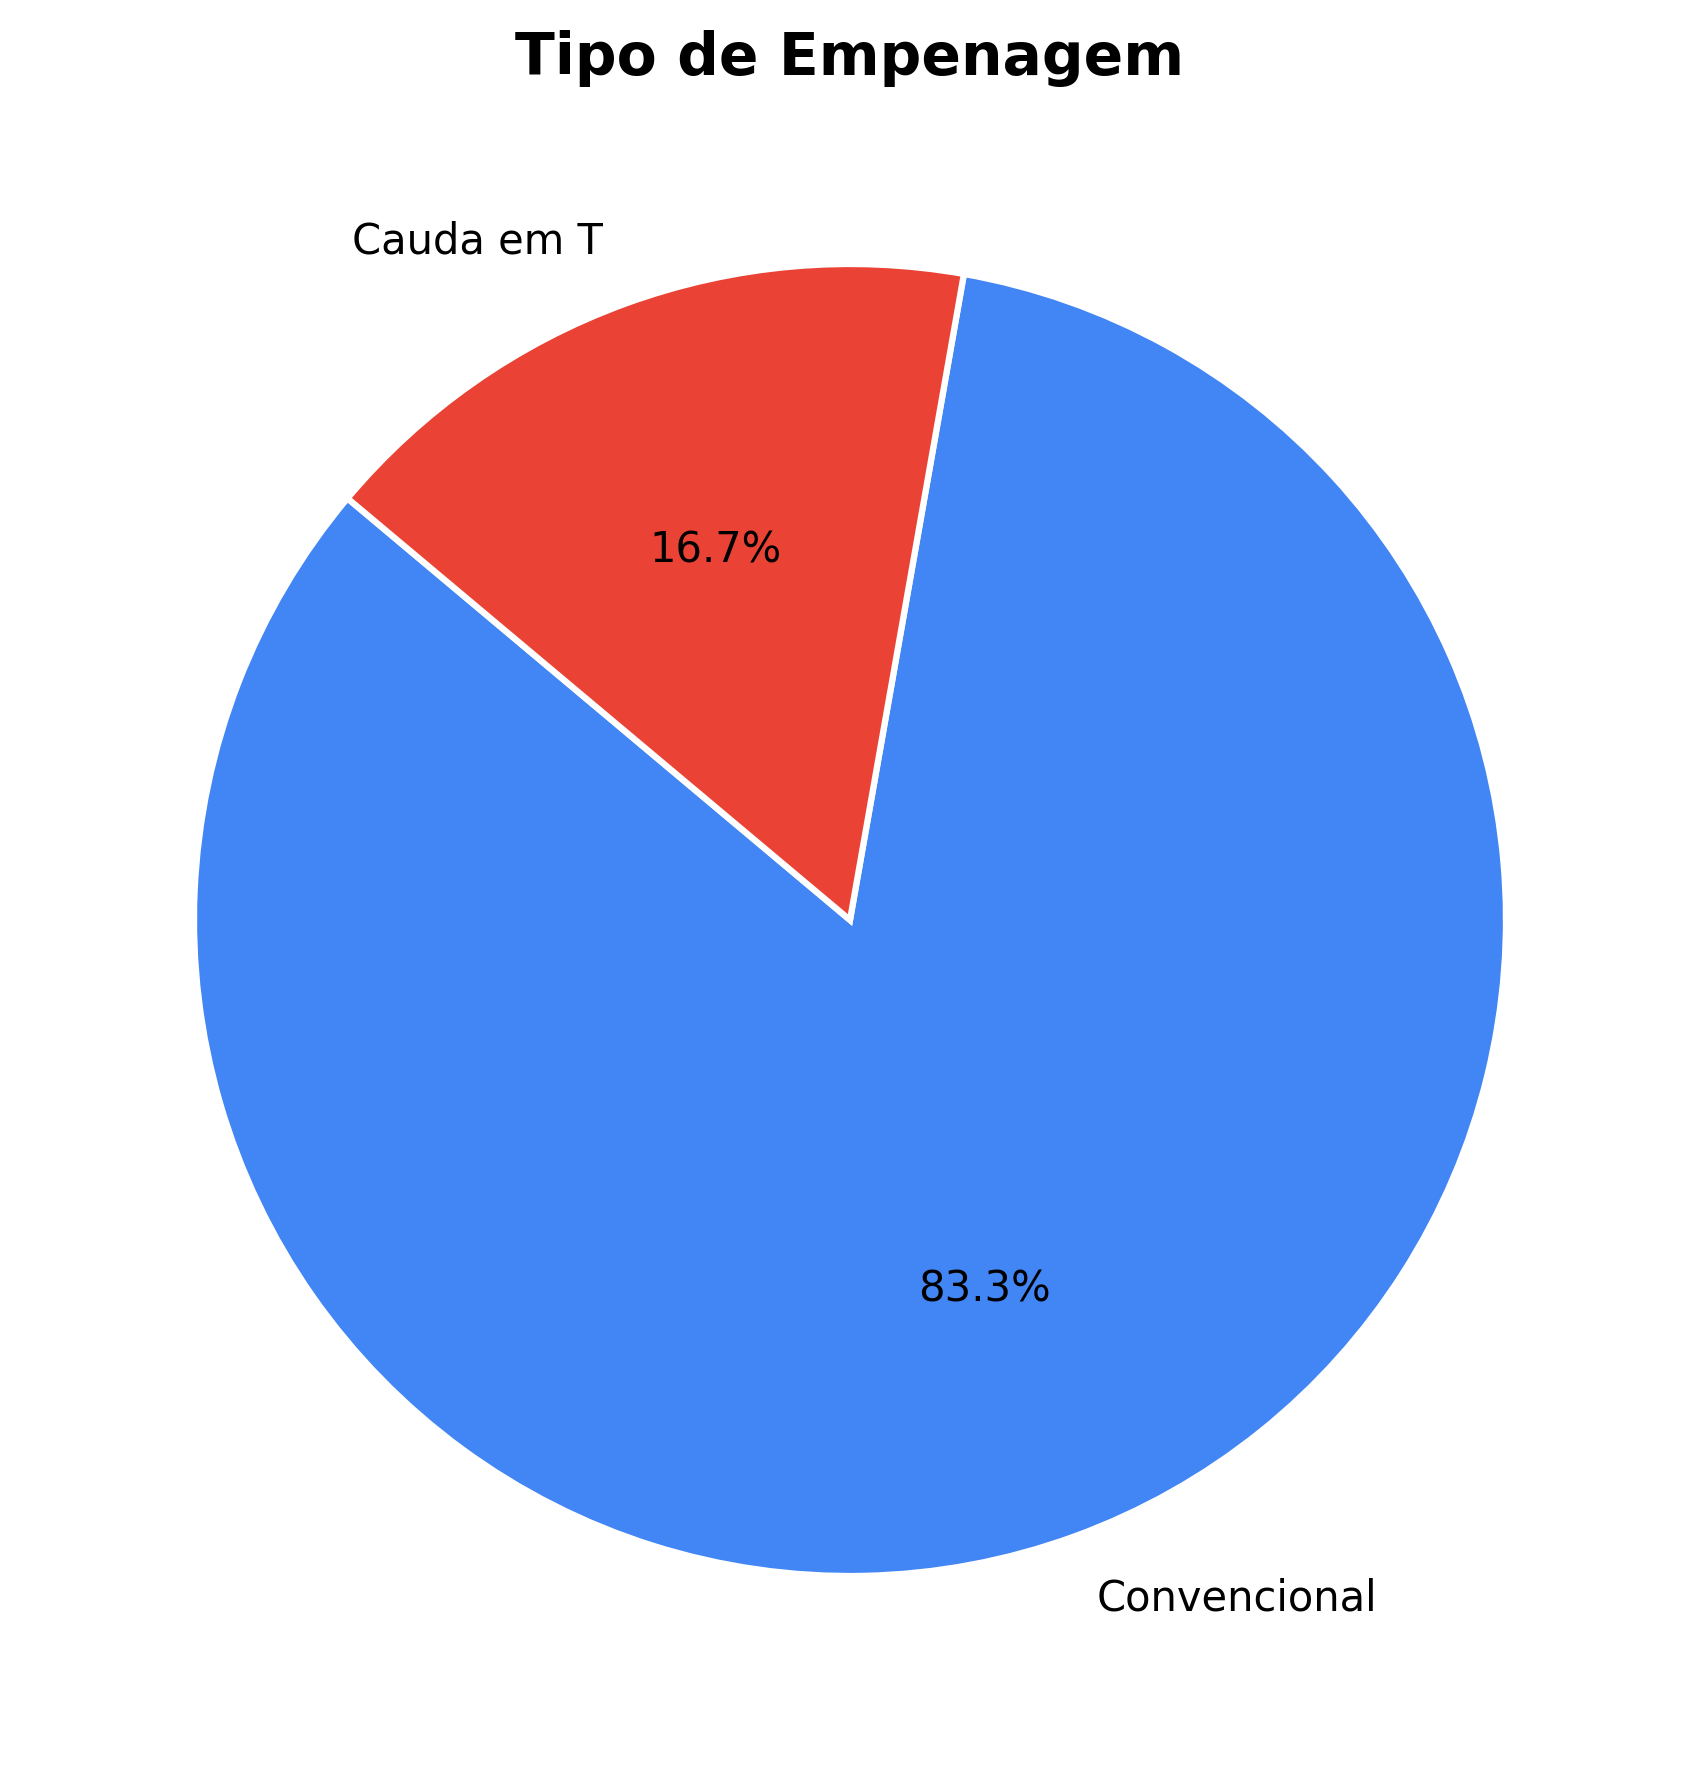
\includegraphics[width=0.6\textwidth]{Images-2-EstudoConceitual/pizza_empenagem.png} 
    \caption{Distribuição do tipo de empenagem entre os concorrentes diretos.}
    \label{fig:tipo_empenage}
\end{figure}

A cauda em T posiciona a empenagem horizontal no topo da empenagem vertical, afastado da esteira da asa e do escoamento das hélices. Em alto ângulo de ataque, porém, a esteira de baixa energia da asa e da fuselagem pode envolver a empenagem horizontal, reduzindo drasticamente a autoridade do profundor e podendo conduzir ao \textit{deep stall}, condição na qual a recuperação por comandos convencionais pode ser comprometida \cite{nguyen2023}. Essa susceptibilidade é agravada pela configuração de asa alta. Para mitigá-la, a cauda em T pode requerer sistemas de prevenção de estol, como o \textit{stick pusher} utilizado no ATR 72-600, com acréscimo de peso, custo de certificação e verificações periódicas.


\begin{figure}[H]
    \centering
    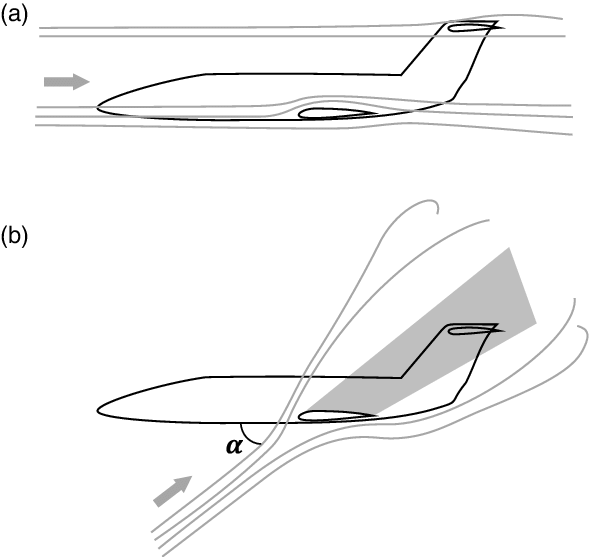
\includegraphics[width=0.7\textwidth]{Images-2-EstudoConceitual/deep_stall_wake.png} 
    \caption{Aeronave de cauda em T (a) em voo normal e (b) em condição de \textit{deep stall}, com a região de esteira de baixa energia da asa (área sombreada) envolvendo a empenagem horizontal em alto ângulo de ataque $\alpha$. Adaptado de \cite{nguyen2023}.}
    \label{fig:deep_stall}
\end{figure}

Na configuração convencional, a empenagem horizontal é fixada ao cone de cauda e permanece abaixo da esteira da asa em alto ângulo de ataque. Isso preserva a autoridade do profundor e favorece a recuperação natural do estol, dispensando sistema dedicado de prevenção. Os carregamentos das empenagens horizontal e vertical ficam desacoplados, o que simplifica o dimensionamento estrutural. Além disso, parte da empenagem horizontal opera no escoamento acelerado pelas hélices, o que aumenta a eficácia do profundor em baixa velocidade e alta potência, condição da decolagem, fase crítica do projeto (distância calculada de 1.102~m contra requisito de 1.280~m). Como contrapartida, a empenagem fica na região de \textit{downwash} da asa, o que exige área ligeiramente maior. Esse efeito é aceito diante dos ganhos descritos. O CASA C-295, de MTOW de 23.200~kgf e com grupo motopropulsor da mesma família deste projeto, adota empenagem convencional.

Dessa forma, a configuração convencional é a escolhida, por dispensar sistema dedicado de prevenção de estol, por favorecer a recuperação inerente do estol e por estar alinhada à tendência das aeronaves de referência. O perfil adotado para a empenagem horizontal é o NACA 0012, simétrico, por não gerar sustentação a ângulo de ataque nulo e por dispor de ampla base de dados experimentais. Para a empenagem vertical, adota-se o NACA 0010, de espessura relativa menor que a do horizontal.





%%%%%%%%%%%%%%%%%%%%%%%%%%%%%%%%%%%%%%%%%%%%%%%%%%%%%%%%%%%%%%%%%%%%%
%%%%%%%%%%%%%%%%%%%%%%%%%%%%%%%%%%%%%%%%%%%%%%%%%%%%%%%%%%%%%%%%%%%%%
%%%%%%%%%%%%%%%%%%%%%%%%%%%%%%%%%%%%%%%%%%%%%%%%%%%%%%%%%%%%%%%%%%%%%

\section{Escolha da Propulsão}

A fim de dimensionar preliminarmente a motorização da aeronave e correlacioná-la com os requisitos de projeto estipulados e com os dados das aeronaves de referência, foram geradas as Figuras \ref{fig:pot_mtow} e \ref{fig:dec_pot}. Neste trabalho, as potências dos motores turboélice são expressas em \textit{shaft horsepower} (SHP), isto é, potência mecânica disponível no eixo do motor.

A Figura \ref{fig:pot_mtow} ilustra a tendência de potência total instalada em função do MTOW na classe de aeronaves estudada. O requisito estabelecido para este projeto prevê um MTOW de 22.680 kgf (indicado pela linha tracejada vermelha). Observando a dispersão estatística e a linha de tendência linear do mercado, conclui-se que o projeto exigirá uma potência total no eixo na faixa de 5.000 a 5.300 shp (aproximadamente 2.500 a 2.650 shp por motor). Este patamar é fundamental para manter a carga de potência ($W/P$) em um nível competitivo e garantir o desempenho em subida.

\begin{figure}[H]
    \centering
    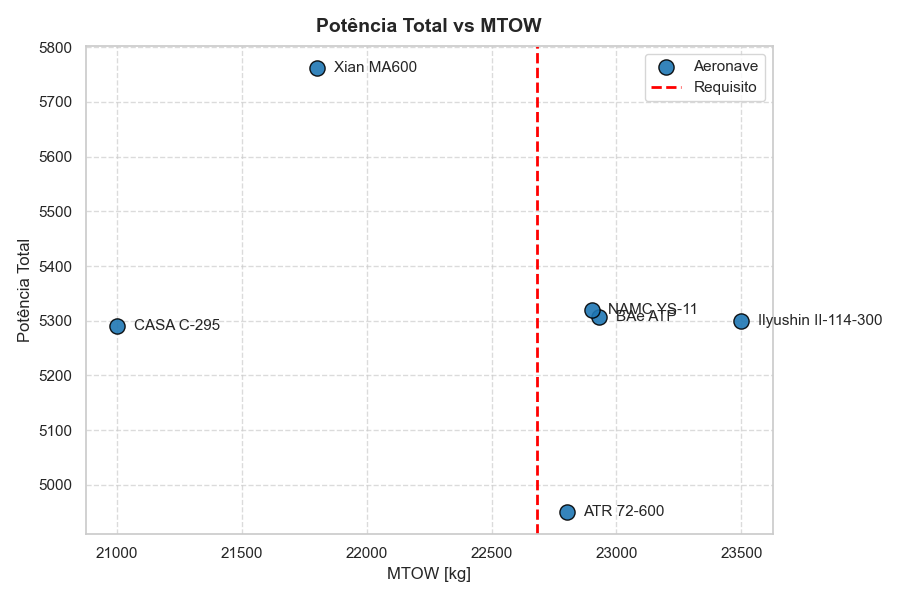
\includegraphics[width=0.75\linewidth]{Images-2-EstudoConceitual/pot_x_mtow.png}
    \caption{Correlação entre Potência Total Instalada e MTOW nos concorrentes diretos.}
    \label{fig:pot_mtow}
\end{figure}

A justificativa para garantir esse nível de potência é diretamente validada pelo rigoroso requisito de decolagem do projeto, estipulado em um comprimento máximo de 1.280 m. A Figura \ref{fig:dec_pot} correlaciona o desempenho de pista das aeronaves de referência com suas respectivas motorizações, evidenciando o limite imposto pelo requisito (linha vermelha tracejada). 

\begin{figure}[H]
    \centering
    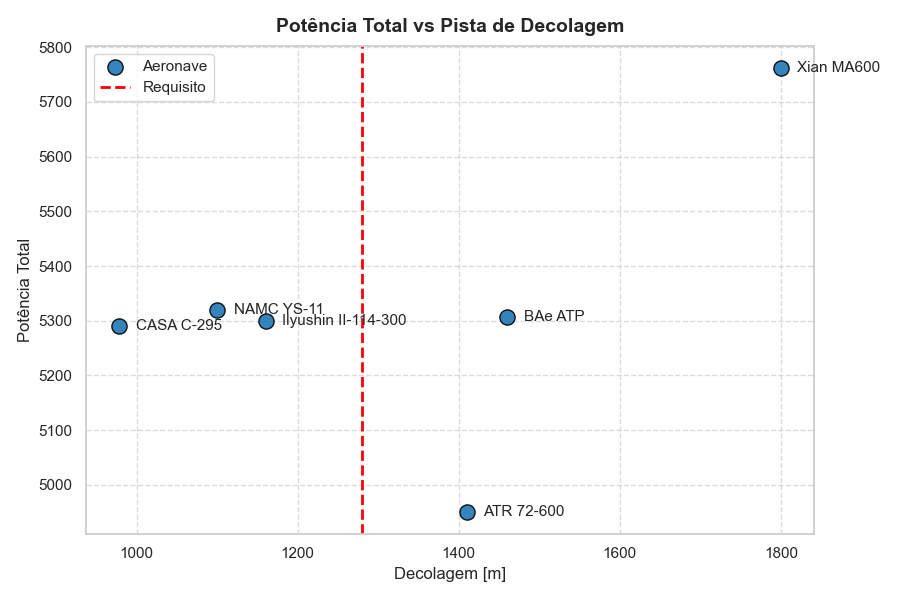
\includegraphics[width=0.75\linewidth]{Images-2-EstudoConceitual/pot_x_decolagem.png}
    \caption{Desempenho de decolagem das aeronaves de referência em função da potência instalada.}
    \label{fig:dec_pot}
\end{figure}

Para garantir que o protótipo opere com folga dentro dos 1.280 m sob condições críticas, a potência estimada na Figura \ref{fig:pot_mtow} precisará atuar em conjunto com um sistema hipersustentador (flaps) de alta eficiência e um conjunto de hélices otimizado para tração estática.

Por fim, o motor selecionado para o projeto da aeronave foi o PW127M, por atender plenamente as necessidades da missão proposta, além de ser da família de motores mais presente nas análises comparativas, o que reforça a confiabilidade e adequação ao projeto. Para além das análises comparativas, o motor da \textit{Pratt \& Whitney} dispõe de relatórios e manuais disponíveis na internet, com informação suficiente para as análises e dimensionamentos posteriores.

Conforme os dados oficiais de certificação estabelecidos no Type Certificate Data Sheet (TCDS) da família PW100 (FAA TCDS nº E20NE / EASA TCDS nº E.070) e no Manual do Fabricante (Part No. 3037332), o motor PW127M é homologado para fornecer uma potência termodinâmica máxima de decolagem de 2.475 shp por unidade. Essa capacidade resulta em uma potência total instalada de 4.950 shp, atendendo plenamente à demanda requerida (entre 5.000 e 5.300 shp, com as devidas margens) para a operação da aeronave nas curtas distâncias de pista estabelecidas pelos requisitos do projeto.

A Tabela~\ref{tab:pw127m} consolida os parâmetros técnicos principais do motor PW127M, confrontando-os com os requisitos de projeto. Nota-se que a potência total instalada de 4.950 shp posiciona a aeronave dentro da faixa prevista pela análise estatística da Figura~\ref{fig:pot_mtow}, e a carga de potência resultante ($W/P \approx 4{,}58$ kg/shp) é competitiva com os concorrentes diretos, em especial o ATR~72-600, cujo motor é o mesmo modelo. 

A combinação do PW127M com as hélices Hamilton Standard 568F, já validadas operacionalmente no ATR~72-600, e com o sistema de flaps dimensionado na seção anterior constitui a solução propulsiva capaz de cumprir o requisito de MTOW e de decolagem.

\begin{table}[H]
  \centering
  \linespread{1}\small
  \setlength{\tabcolsep}{4pt}
  \caption{Parâmetros técnicos do motor selecionado (PW127M) e sua conformidade com os requisitos de projeto.}
  \label{tab:pw127m}
  \begin{tabularx}{\textwidth}{>{\hsize=1.2\hsize}L >{\hsize=0.9\hsize}C >{\hsize=0.9\hsize}C}
    \toprule
    \textbf{Parâmetro} & \textbf{Valor} & \textbf{Requisito / Referência} \\
    \midrule
    Fabricante & Pratt \& Whitney Canada & --- \\
    Modelo & PW127M & --- \\
    Tipo & Turboélice & Turboélice (seção 3.2.4) \\
    Número de motores & 2 & 2 (seção 3.2.4) \\
    Potência máx.\ de decolagem (por motor) & 2.475 shp & $\geq$ 2.500 shp (est.) \\
    Potência total instalada & 4.950 shp & 5.000--5.300 shp (Fig.~\ref{fig:pot_mtow}) \\
    Peso seco por motor & 480,8 kgf (1.060 lb) & --- \\
    Carga de potência ($W/P$) & 4,58 kg/shp & Compatível com concorrentes \\
    Hélice & Hamilton Standard 568F & --- \\
    Pista de decolagem estimada & $\leq$ 1.280 m & $\leq$ 1.280 m (seção 2.1) \\
    Velocidade de cruzeiro compatível & 260 kt & 260 kt (seção 2.1) \\
    Teto de serviço compatível & FL250 & FL250 (seção 2.1) \\
    \bottomrule
  \end{tabularx}
\end{table}

Definido o conjunto motopropulsor deste projeto (motor PW127M acoplado à hélice Hamilton Standard 568F de 6 pás), cabe justificar tecnicamente essa escolha frente à alternativa de 4 pás, historicamente empregada em variantes de menor potência da mesma família de referência. De forma que essa decisão impacta diretamente a eficiência propulsiva, nível de ruído e vibração de cabine, peso do grupo  motopropulsor e a integridade estrutural da pá frente a efeitos de compressibilidade. A Tabela \ref{tab:comparativo_pas} sintetiza a comparação técnica entre as duas configurações consideradas.

\begin{table}[H]
  \centering
  \linespread{1}\small
  \setlength{\tabcolsep}{4pt}
  \caption{Comparativo entre hélices de 4 e 6 pás para a faixa de potência do projeto.}
  \label{tab:comparativo_pas}
  \begin{tabularx}{\textwidth}{L L L}
    \toprule
    \textbf{Critério} & \textbf{4 pás} & \textbf{6 pás} \\
    \midrule
    Peso do conjunto rotativo & Menor & Maior \\
    Complexidade/custo de manutenção & Menor & Maior \\
    Absorção de potência (diâmetro fixo) & Limitada & Adequada \\
    Velocidade de ponta / compressibilidade & Prejudicial em alta potência & Mitigada \\
    Ruído e vibração de cabine & Maior & Menor (37, 38) \\
    Precedente na potência do projeto & ATR 72-200, PW124B ($\sim$2.400 shp) & ATR 72-500/600, PW127 ($\sim$2.475--2.750 shp) \\
    \bottomrule
  \end{tabularx}
\end{table}

Assim, a configuração de 4 pás apresenta vantagens de peso, custo e complexidade mecânica, que, no entanto, são características de motores na faixa de 2.000--2.400 shp por unidade, como o PW124B utilizado no ATR 72-200 com hélices Hamilton Standard 14SF-11. Para a potência efetivamente instalada neste projeto (motor PW127M), certificado sob a TCDS E20NE da FAA para a família PW100, com 2.475 shp por motor (Tabela \ref{tab:pw127m}), os critérios que passam a dominar a decisão são aqueles em que a configuração de 6 pás se sobressai: capacidade de absorção de potência sem penalizar a velocidade de ponta e o ruído de cabine. Esse comportamento é consistente com a evolução real da família ATR, que substituiu a hélice de 4 pás pela Hamilton Standard 568F de 6 pás ao migrar do PW124B para o PW127M, mantendo o diâmetro praticamente inalterado conforme a TCDS P8BO da Hamilton Sundstrand Corp. e o comunicado técnico da Collins Aerospace, atual fabricante do conjunto, que reporta mais de 30 milhões de horas de voo em serviço nessa configuração de 6 pás na frota ATR 42/72.

Para uma dada rotação, uma hélice absorve mais potência apenas por dois caminhos: aumentar o diâmetro (elevando diretamente a componente rotacional da velocidade de ponta, $V_{rot} = \pi \cdot D \cdot N$) ou aumentar a solidez do disco, absorvendo mais potência sem penalizar essa velocidade. Utilizando os dados de diâmetro e rotação de referência da hélice 568F ($D = 3{,}93$ m; $N \approx 1200$ rpm a 100\% $N_p$, conforme especificação do fabricante do motor (36)) na condição de cruzeiro do projeto ($V_{cruise} = 260$ kt; FL250 -- Tabela \ref{tab:pw127m}), obtém-se:

\begin{equation}
    V_{rot} = \pi \cdot D \cdot N = \pi \cdot 3{,}93 \cdot \left(\frac{1200}{60}\right) 
\approx 247 \text{ m/s}
    \label{eq:vrot}
\end{equation}

\begin{equation}
    V_{ponta} = \sqrt{V_{rot}^2 + V_{cruise}^2} = \sqrt{247^2 + 133{,}8^2} 
    \approx 281 \text{ m/s}
    \label{eq:vponta}
\end{equation}

Para a atmosfera padrão ISA em FL250 ($T \approx 238{,}7$ K), a velocidade do som é $a \approx 310$ m/s, resultando em um número de Mach de ponta de pá de:

\begin{equation}
    M_{ponta} = \frac{V_{ponta}}{a} \approx 0{,}91
    \label{eq:mach_ponta}
\end{equation}

Esse valor já se encontra próximo do limite prático de operação subsônica na ponta da pá, mesmo com 6 pás absorvendo a potência do PW127M. Caso a mesma potência fosse absorvida por apenas 4 pás no mesmo diâmetro, seria necessário aumentar a corda/espessura de cada pá para preservar a área projetada total, elevando a aceleração local do escoamento, aumentando ainda mais esse número de Mach efetivo. Alternativamente, aumentar o diâmetro eleva diretamente $V_{rot}$ na Equação \ref{eq:vrot} e, consequentemente, $V_{ponta}$ na Equação \ref{eq:vponta}. Esse comportamento apresenta perdas por compressibilidade e aumento de ruído tonal proporcionais ao número de Mach helicoidal de ponta como apresentado na literatura técnica sobre hélices de alta velocidade.

Diante do exposto na Tabela \ref{tab:comparativo_pas} e da verificação quantitativa acima, mantém-se a adoção da hélice Hamilton Standard 568F de 6 pás para este projeto. Embora a configuração de 4 pás seja tecnicamente superior em peso e custo, ela é adequada apenas à faixa de potência de motores como o PW124B, inferior à do PW127M a ser adotado. Para a potência e o diâmetro que caracterizam esta aeronave, a configuração de 6 pás é a que melhor concilia absorção de potência, integridade estrutural da pá e conforto de cabine, replicando a mesma solução já validada operacionalmente pela família ATR 72-500/600 nessa exata faixa de potência.

\subsection{Integração da Hélice e Distância ao Solo}
\label{sec:selecao_pas}

Para garantir a segurança operacional e o cumprimento dos requisitos de certificação, procedeu-se à verificação da distância vertical entre a ponta da pá da hélice e o solo (ground clearance). O \S 25.925(a) do 14 CFR Part 25 determina que, para aeronaves com trem de pouso triciclo, a distância mínima entre a hélice e o solo deve ser de pelo menos 7 polegadas (178 mm) com a aeronave estática no peso máximo.  

Na configuração adotada para esta aeronave de asa alta, a linha de centro dos motores (eixo da hélice) encontra-se alinhada ao topo da fuselagem. Sabendo que o diâmetro da fuselagem é de 2.900 mm e a altura estática do trem de pouso dimensionado é de 700 mm, a altura total do eixo do motor em relação ao solo é de 3.600 mm.  A hélice selecionada, Hamilton Standard 568F, possui um diâmetro de 3,93 m, o que resulta em um raio de 1.965 mm. A distância vertical da ponta da pá ao solo é calculada subtraindo-se o raio da hélice da altura do eixo do motor: 

$Clearance = H_{motor} - R_{prop}$

$Clearance = 3.600 \text{ mm} - 1.965 \text{ mm} = 1.635 \text{ mm} \text{ (ou } 1,635 \text{ m)}$

O valor obtido de 1.635 mm supera o mínimo normativo de 178 mm. Essa folga vertical é uma vantagem do projeto, pois mitigará o risco de ingestão ou impacto de detritos, uma característica fundamental para uma aeronave regional projetada para operar em aeroportos com infraestrutura limitada ou pistas semi-preparadas.

\subsection{Segurança, Marcação e Posicionamento do Disco da Hélice}
\label{sec:seguranca_helice}

No que tange à segurança e certificação, o posicionamento das hélices Hamilton Standard 568F foi avaliado frente a cenários de falha catastrófica (como a perda de uma pá) e ao desprendimento de gelo (ice shedding). Conforme o \S 25.903(d) do 14 CFR Part 25, o projeto deve minimizar os riscos aos ocupantes em caso de falha de rotores.

Analisando o arranjo geral da aeronave, o plano de rotação do disco da hélice cruza a fuselagem na zona de serviço dianteira, região que abriga o lavatório e os compartimentos de bagagem. Essa disposição geométrica é altamente vantajosa, pois o plano do disco não intercepta diretamente a cabine de comando (cockpit) nem as fileiras de assentos dos passageiros. Para mitigar o impacto de blocos de gelo desprendidos das pás pela força centrífuga, a seção da fuselagem alinhada ao disco da hélice deverá ser estruturalmente reforçada com a instalação de painéis externos de impacto (ice shields).

Adicionalmente, para garantir a segurança das equipes de apoio e handling durante as operações em solo com os motores em funcionamento, são adotadas medidas de sinalização visual padronizadas. As pontas das pás das hélices receberão pintura de segurança em cores de alto contraste (faixas concêntricas de amarelo, preto e branco ou vermelho e branco), criando um arco visual contínuo e facilmente identificável quando em rotação. Em complemento, a superfície externa da fuselagem receberá marcações de aviso com faixas verticais vermelhas ladeando o plano do disco, acompanhadas da inscrição "PROPELLER" e setas de advertência, em conformidade com as exigências de segurança de rampa.

\chapter{Estudo de Conversão}

\section{Análise de Aeronaves de Referência}

O desenvolvimento do conceito de operação em missão dupla exige uma arquitetura de cabine que minimize o tempo de pátio durante o processo de reconfiguração. Na análise de projetos consolidados, observam-se filosofias distintas para a solução deste problema.

Aeronaves regionais civis tradicionais, como o ATR-72, quando adaptadas para operações de carga ou conversões rápidas, dependem da extração de assentos e inserção de cargas através de portas laterais. Na versão \textit{Quick Change} ou nos layouts convertíveis do ATR-72, o processo logístico exige a movimentação de componentes unitários através de aberturas dispostas lateralmente na fuselagem. O processo oficial de conversão de cabine leva em torno de uma hora no ATR-72, sendo frequentemente planejado como um procedimento para as janelas noturnas.

Em geral, no procedimento de conversão, a equipe de solo inicia com a desmontagem manual de elementos de cabine, como os painéis de divisão, as redes de contenção e o assento dianteiro do comissário. Após o destravamento mecânico das fileiras de assentos, que são instaladas de modo convencional nos trilhos do piso, estas fileiras são transladadas manualmente ao longo do corredor central em direção às saídas operacionais. A remoção das poltronas para o exterior e a inserção da carga paletizada ocorre através de uma porta de carga alargada (conhecida como \textit{Large Cargo Door}). Esta porta dispõe de uma soleira rebaixada a uma certa altura do solo para facilitar o recebimento dos contêineres otimizados.  

Embora o sistema QC atenda às normas e permita ao ATR acomodar ULDs no main deck, a cinemática de conversão por portas laterais exigem que os assentos e paletes extraídos precisem ser rotacionados em 90 graus no interior da aeronave antes de passarem pelo vão da porta, o que demanda maior intervenção braçal e expõe o revestimento interno a danos.

Tomando como outro exemplo a aeronave CASA C-295, originada como um cargueiro tático, apresenta uma arquitetura intrinsecamente modular, resolvendo o gargalo direcional através de uma rampa traseira e um piso plano provido de um sistema contínuo de roletes e pontos de fixação compatíveis com paletes. A transição total da cabine de carga para uma configuração completa e segura de passageiros ou transporte aeromédico pode ser finalizada em menos de 2 horas.

Em geral, os assentos de passageiros são fixados previamente de forma integral sobre plataformas padronizadas de assoalho (como o sistema multibase), juntamente com equipamentos auxiliares de oxigênio e segurança. A montagem estrutural de cada palete fora da aeronave é rápida, exigindo apenas dois operadores e cerca de 20 minutos. Para a inserção, a rampa traseira principal atua como a interface direta entre o nível de carregamento e a cabine, podendo operar nivelada com equipamentos de rampa de solo. O translado logístico dos grandes paletes modulares é realizado com o auxílio de um guincho mecânico no interior da cabine. Finalmente, os paletes contendo os assentos são fixados de modo consolidado no piso, sem a necessidade de acoplar as fileiras individualmente.

Essa solução longitudinal ininterrupta suprime a extração avulsa e contorna as limitações de rotação das portas laterais. Contudo, é importante ponderar as penalidades de projeto inerentes a esta arquitetura. A necessidade de uma rampa traseira pressurizável e de um assoalho com trilhos estruturais eleva substancialmente o peso vazio operacional (OEW) da aeronave, além de o formato elevado da cauda impor um incremento considerável de arrasto aerodinâmico de base.

\section*{Escolha e Justificativa da Arquitetura de Carregamento}

Para este projeto, optou-se pela implementação de uma porta de carga lateral (\textit{Large Cargo Door} - LCD) em detrimento de uma rampa de carregamento traseira. Do ponto de vista da integração estrutural, a porta lateral é significativamente mais simples de projetar e manufaturar, pois preserva a geometria cilíndrica convencional da fuselagem. A adoção de uma porta traseira exigiria o projeto de um cone de cauda elevado, o que não apenas incrementa o arrasto aerodinâmico de base, mas também pode alterar de forma indesejada as derivadas de estabilidade e a controlabilidade direcional e longitudinal da aeronave, exigindo um redimensionamento complexo da empenagem.

Adicionalmente, a filosofia de carregamento deve estar estritamente alinhada com o perfil da dupla missão proposta. Rampas traseiras, embora otimizem o tempo de transição, são mandatórias primordialmente para cargas indivisíveis de grande porte ou veículos táticos. Para uma aeronave comercial de transporte regional, cujas cargas consistem essencialmente em paletes padronizados e contêineres ULDs, a porta lateral se mostra a solução mais coerente. Essa escolha simplifica consideravelmente o planejamento aeroportuário, garantindo compatibilidade imediata com a infraestrutura civil existente e permitindo o uso de elevadores de carga e Equipamentos de Apoio no Solo (GSE) convencionais, amplamente disponíveis em aeroportos regionais.

Apesar da adoção da porta lateral, a filosofia de \textit{Quick Change} baseada no deslizamento longitudinal será mantida para maximizar a modularidade da cabine. As fileiras de assentos permanecerão fixadas aos trilhos estruturais do piso. Durante a conversão, os módulos de assentos serão destravados e transladados ao longo do corredor até a seção da porta. Para efetivar a transição física dos assentos e cargas entre o \textit{main deck} e o pátio, a operação dependerá da interface com plataformas elevatórias externas ou rampas móveis posicionadas ao lado da aeronave, compensando a ausência de uma rampa integrada sem penalizar o peso vazio operacional (OEW).

Por fim, é imperativo destacar as mitigações operacionais necessárias inerentes a esta arquitetura. A cinemática de carregamento por porta lateral exige uma inevitável mudança de direção: uma rotação de 90 graus dos paletes e módulos de assentos no interior da aeronave antes da extração. Consequentemente, a área do piso adjacente à porta deverá ser equipada com painéis de transferência omnidirecional e a equipe de \textit{handling} deverá adotar procedimentos rigorosos para evitar impactos e danos estruturais ao revestimento interno durante as manobras logísticas.

\section{Esboços Iniciais}

A seguir, são apresentadas as vistas principais da aeronave. Ressalta-se que essas representações correspondem a um esboço inicial do projeto, tendo como objetivo fornecer uma visualização preliminar da geometria.

% --- VISTA SUPERIOR ---
\begin{figure}[H]
    \centering
    \begin{minipage}{0.8\textwidth} % Ajuste o 0.8 para aumentar ou diminuir o tamanho
        \centering
        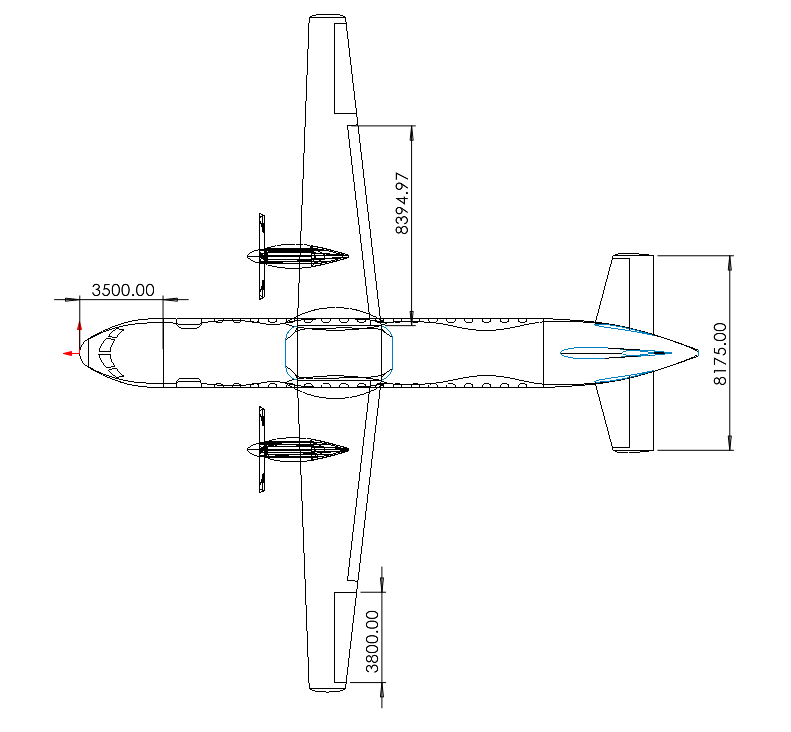
\includegraphics[width=\linewidth]{Images-2-EstudoConceitual/vista_superior.png}
        \caption{Esboço da vista superior da aeronave.}
        \label{fig:vista_superior}
    \end{minipage}
\end{figure}

% --- VISTA LATERAL ---
\begin{figure}[H]
    \centering
    \begin{minipage}{0.8\textwidth}
        \centering
        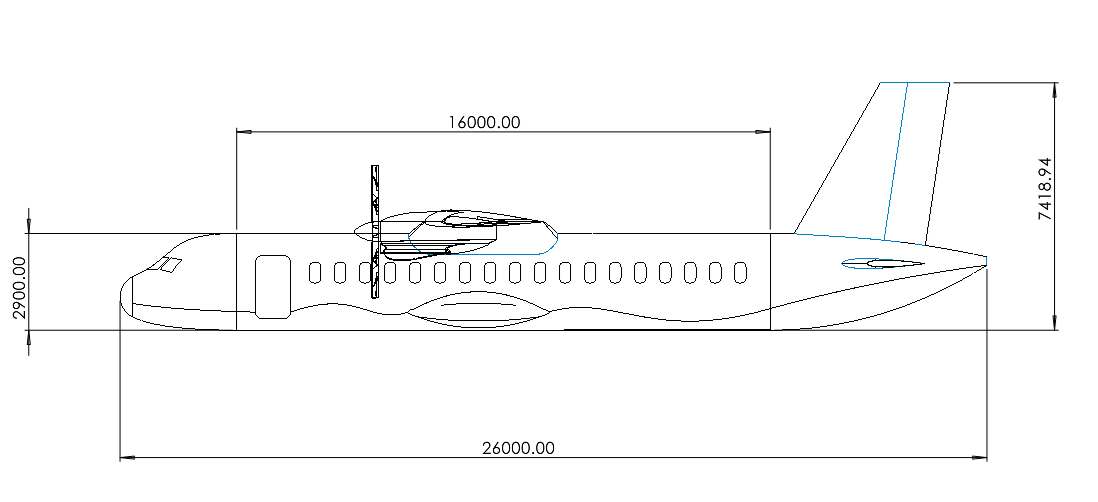
\includegraphics[width=\linewidth]{Images-2-EstudoConceitual/vista_lateral.png}
        \caption{Esboço da vista lateral da aeronave.}
        \label{fig:vista_lateral}
    \end{minipage}
\end{figure}

% --- VISTA FRONTAL ---
\begin{figure}[H]
    \centering
    \begin{minipage}{0.8\textwidth}
        \centering
        \includegraphics[width=\linewidth]{Images-2-EstudoConceitual/vista_frontal.png}
        \caption{Esboço da vista frontal da aeronave.}
        \label{fig:vista_frontal}
    \end{minipage}
\end{figure}

% --- VISTA ISOMÉTRICA (SEPARADA/DESTAQUE) ---
\begin{figure}[H]
    \centering
    \begin{minipage}{0.9\textwidth} % Isométrica levemente maior para destaque
        \centering
        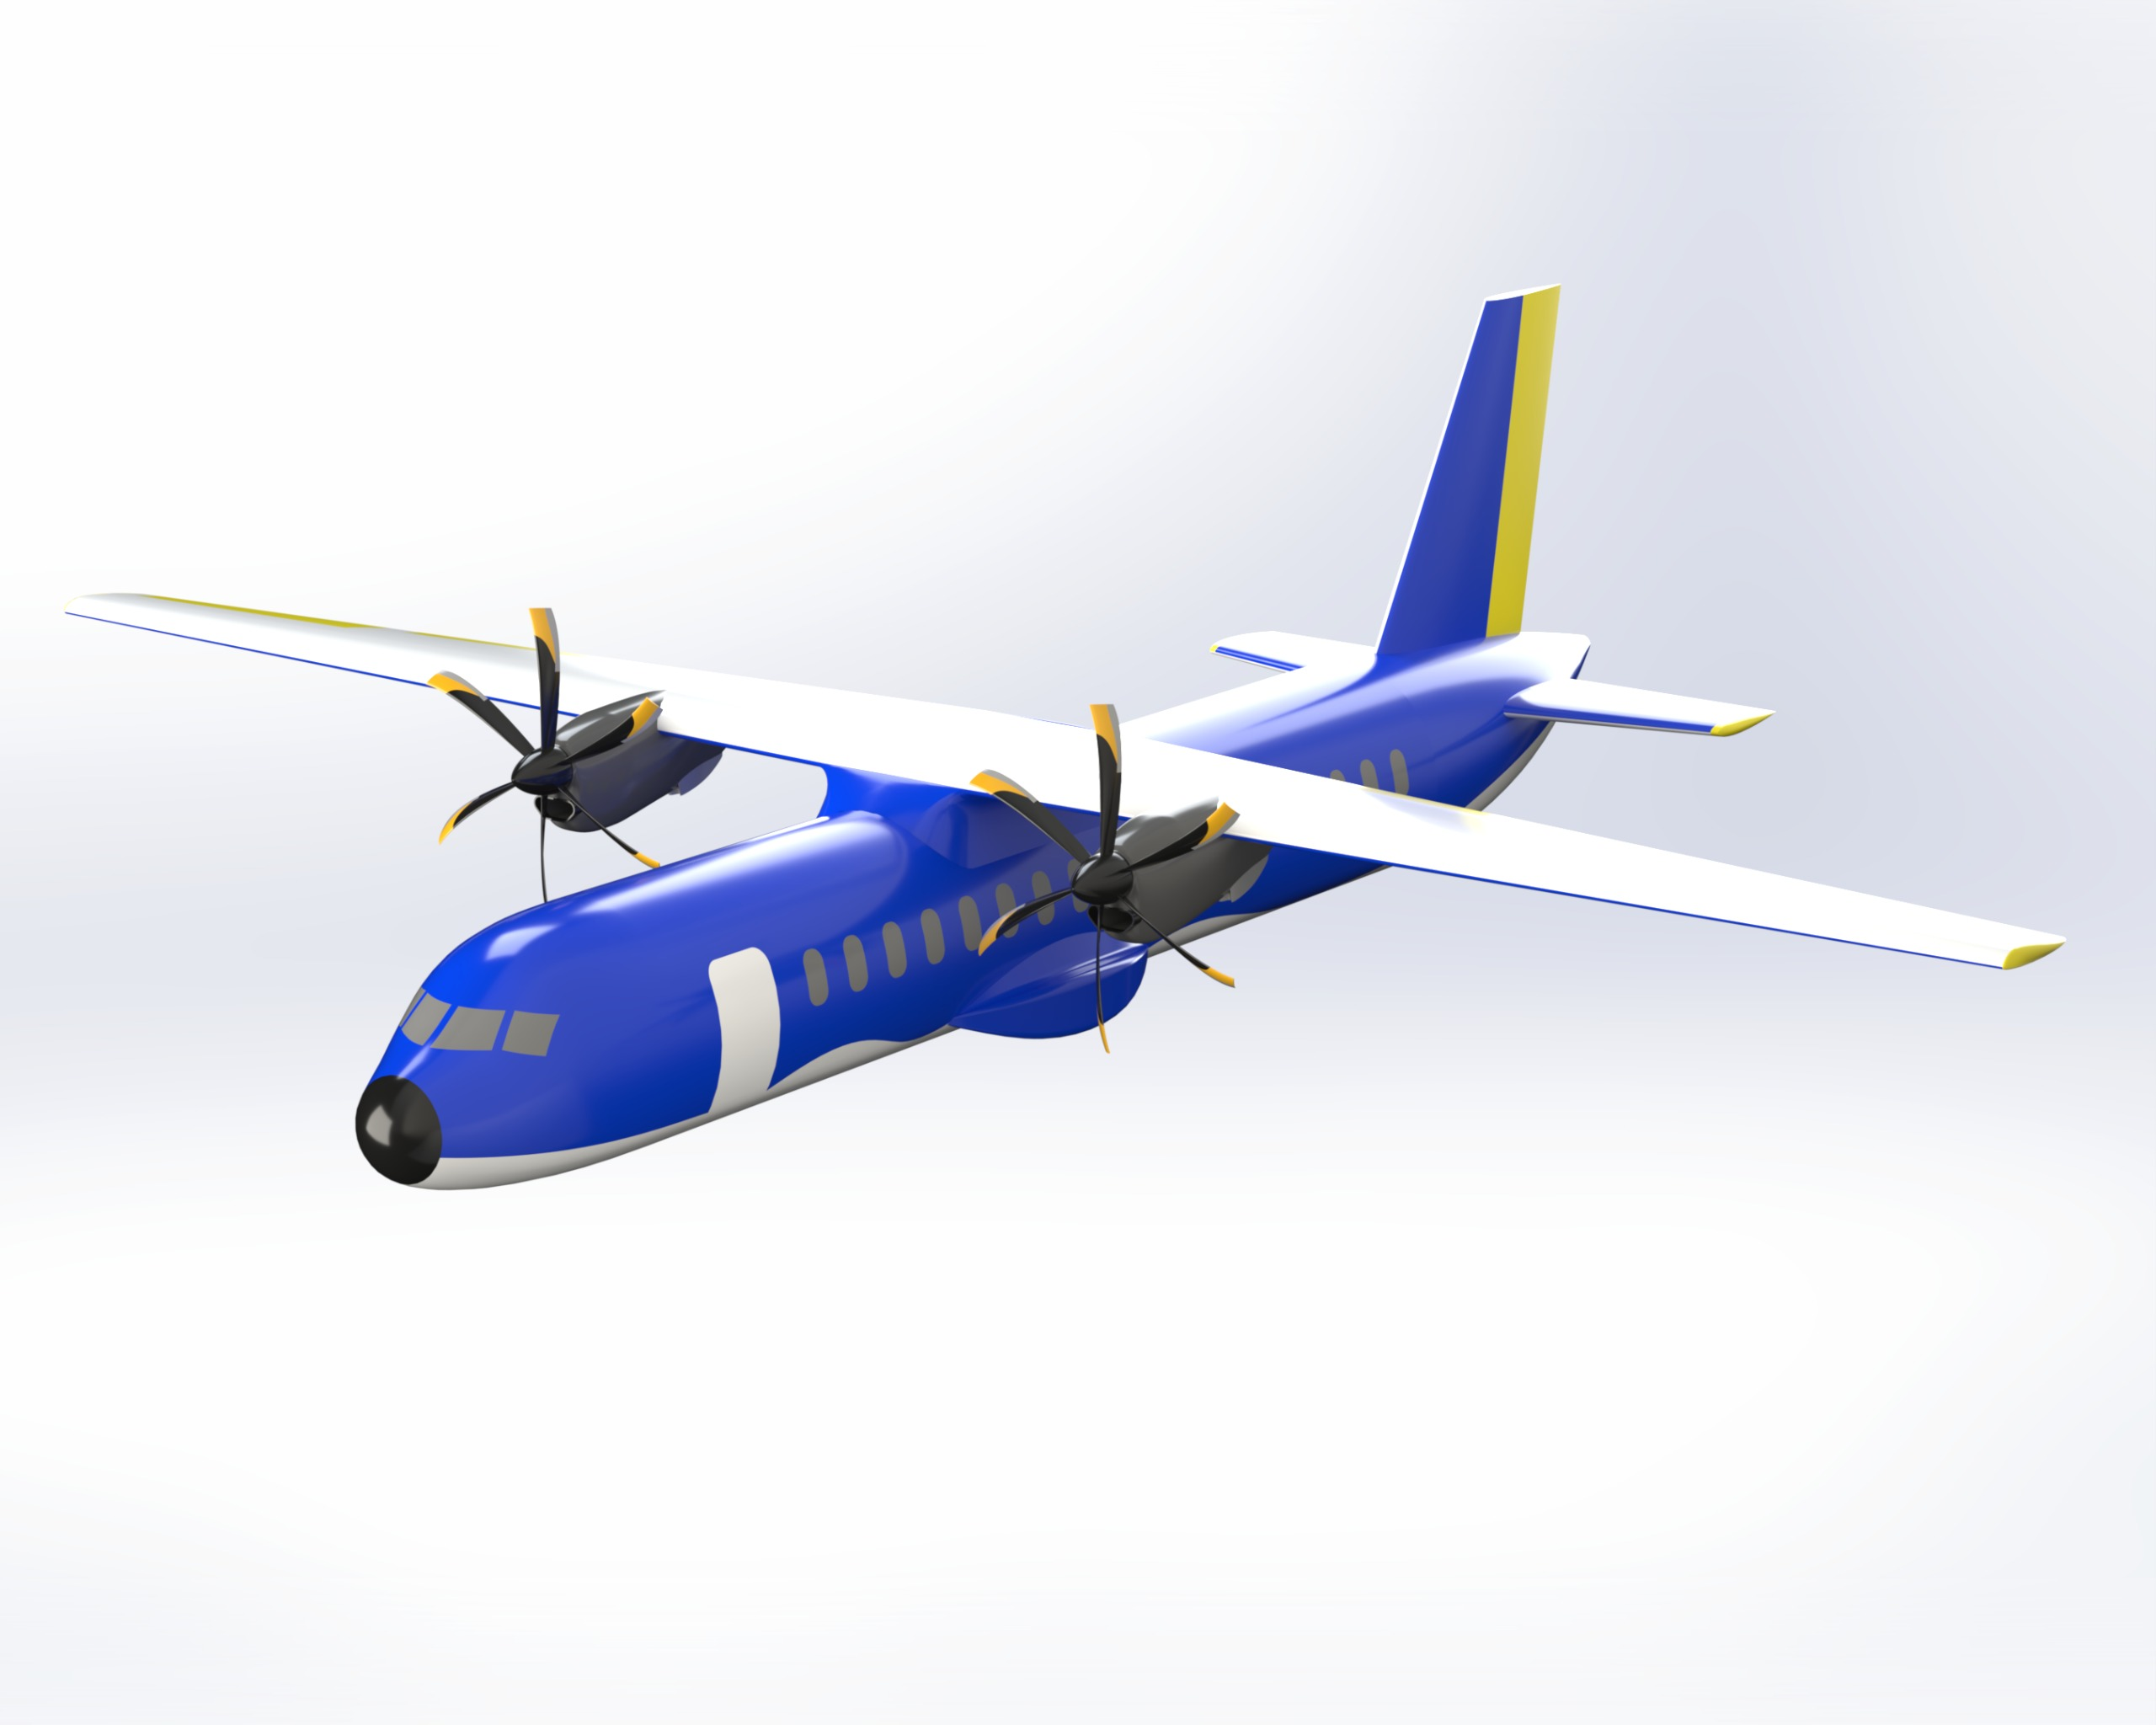
\includegraphics[width=\linewidth]{Images-2-EstudoConceitual/vista_isometrica.png}
        \caption{Vista isométrica preliminar apresentando a configuração geral e livery inicial.}
        \label{fig:vista_isometrica}
    \end{minipage}
\end{figure}
\chapter{Conclusão do Anteprojeto}
 Os valores para as dimensões do projeto dessa aeronave, a partir da análise comparativa, da teoria apresentada e dos requisitos estão na tabela \ref{tab:dimensoes_conclusao}.

\begin{table}[H]
\centering
\caption{Dimensões definidos para o projeto.}
\label{tab:dimensoes_conclusao}
\resizebox{0.7\textwidth}{!}{%
\begin{tabular}{l|c}
\hline
\textbf{Dimensão} & \textbf{Valor} \\ \hline
b & 28,5 m \\ \hline
Corda da raiz & 3,7 m \\ \hline
Corda da ponta & 1,5 m \\ \hline
$\Lambda$ & 0 [$^\circ$] \\ \hline
$\Gamma$ & 2,81 [$^\circ$] \\ \hline
$\lambda$ & 0,405 \\ \hline
Alongamento & 10,96 \\ \hline
Área alar & 74,1 $m^2$\\ \hline
Corda média aerodinâmica & 2,75 m \\ \hline
Aileron & 3,8 m (comp.) / 0,92 m (larg.) \\ \hline
Flap & 8,7 m (comp.) / 0,44 m (larg.) \\ \hline
$t_r$ & 2,185 ft \\ \hline
$l_f$ & 85,3 ft \\ \hline
$w_f + h_f$ & 18,18 ft \\ \hline
$b_{HT}$ & 8,375 m \\ \hline
$S_{HT}$ & 18,679 m$^2$ \\ \hline
$\lambda_{HT}$ & 0,60 \\ \hline
$c_{raiz, HT}$ & 2,788 m \\ \hline
$c_{ponta, HT}$ & 1,673 m \\ \hline
$\Lambda_{HT}$ & 8,5$^\circ$ \\ \hline
$\Gamma_{HT}$ & 0,0$^\circ$ \\ \hline
$l_{HT}$  & 12,00 m \\ \hline
$V_{HT}$ & 1,10 \\ \hline
$c_{e}$ & 30\% da $cma$ \\ \hline
$b_{VT}$ & 4,925 m \\ \hline
$S_{VT}$ & 15,359 m$^2$ \\ \hline
$\lambda_{VT}$ & 0,50 \\ \hline
$c_{raiz, VT}$ & 4,158 m \\ \hline
$c_{ponta, VT}$ & 2,079 m \\ \hline
$\Lambda_{VT}$ & 25,0$^\circ$ \\ \hline
$\Gamma_{VT}$ & 0,0$^\circ$ \\ \hline
$l_{VT}$ & 11,00 m \\ \hline
$V_{VT}$ & 0,08 \\ \hline
$c_{r}$ & 30\% da $cma$  \\ \hline
\end{tabular}%
}
\end{table}

\chapter{Projeto Preliminar}

\section{Definição do Perfil da Asa}

Inicialmente, foram identificados os perfis utilizados nas aeronaves de referência, conforme a Tabela \ref{tab:perfiscomparativos}. Os dados foram obtidos no \textit{The Incomplete Guide to Airfoil Usage} \cite{uiuc_airfoil_database}, exceto para o Xian MA600, para o qual foi utilizada a referência da Antonov Company sobre o An-24 \cite{antonov_an24}. Não foi encontrada uma fonte confiável para o perfil do Ilyushin Il-114-300.

\begin{table}[H]
\centering
\caption{Perfis aerodinâmicos das aeronaves analisadas.}
\label{tab:perfiscomparativos}
\begin{tabular}{|l|c|c|}
\hline
\textbf{Aeronave} & \textbf{Perfil na Raiz} & \textbf{Perfil na Ponta} \\ \hline
ATR-72 & NACA 43018 Modificado & NACA 43013 Modificado  \\ \hline
CASA C-295 & NACA 65-218 & NACA 65-218 \\ \hline
British Aerospace ATP & NACA 23018 & NACA 4412 \\ \hline
NAMC YS-11 & NACA 64A218 & NACA 64A412 \\ \hline
Xian MA600 & TsAGI S-5-18 & TsAGI S-3-13 \\ \hline
\end{tabular}
\end{table}

Entre as aeronaves analisadas, observa-se a utilização de perfis NACA de cinco dígitos em projetos de referência, como o ATR-72 e o British Aerospace ATP. Essa família foi adotada como ponto de partida para o presente projeto. Sua nomenclatura é definida por:

\begin{itemize}
    \item O primeiro dígito multiplicado por 0,15 define o coeficiente de sustentação de projeto. Para o NACA 43018, $C_l = 4 \cdot 0,15 = 0,60$;
    \item O segundo e o terceiro dígitos estão associados à posição de máxima curvatura. Para o NACA 43018, o número 30 corresponde a $15\%$ da corda;
    \item O terceiro dígito igual a 0 indica uma linha média convencional, não reflexa;
    \item Os dois últimos dígitos representam a espessura relativa máxima, resultando em $t/c=18\%$.
\end{itemize}

A seguir, estima-se o coeficiente de sustentação de projeto para a condição de cruzeiro.

\subsection{Análise de Condição de Cruzeiro}

Considerando cruzeiro a 20.000 ft, equivalente a 80\% do teto operacional, o coeficiente de sustentação é estimado por:

\begin{equation}
\label{eq:ClCruseiro}
    C_{l_{cruise}} = \frac{MTOW \cdot g}{\frac{1}{2}\rho_{cruise} V_{cruise}^2 S_{wing}} = 0,48
\end{equation}
Onde o $MTOW = 22680 \ kg$, $V_{cruise} = 260 \ kt$, $S = 74,1 \ m^2$.

Com o valor obtido pela Eq. \ref{eq:ClCruseiro}, podemos estimar o coeficiente que o perfil aerodinâmico deve gerar levando em conta efeitos tridimensionais e de perfil ideal, tal que Raymer \cite{raymer2018} indica:

\begin{equation}
\label{eq:Clperfildeverdade}
    C_l = C_{l_{cruise}}/0,86 = 0,56
\end{equation}

\subsection{Comparação de Eficiência Aerodinâmica}
\label{subsec:comparacao_ld_perfis}

Para $C_l \approx 0,56$, comparou-se o NACA 43018, utilizado como representante preliminar da família NACA 430XX, com os perfis laminares NACA 64-215 e NACA 65(2)-215. As polares foram obtidas no AirfoilTools \cite{airfoiltools} e a comparação de $C_l/C_d$ é apresentada na Figura \ref{fig:comparacao_clcd_cl}.

\begin{figure}[H]
    \centering
    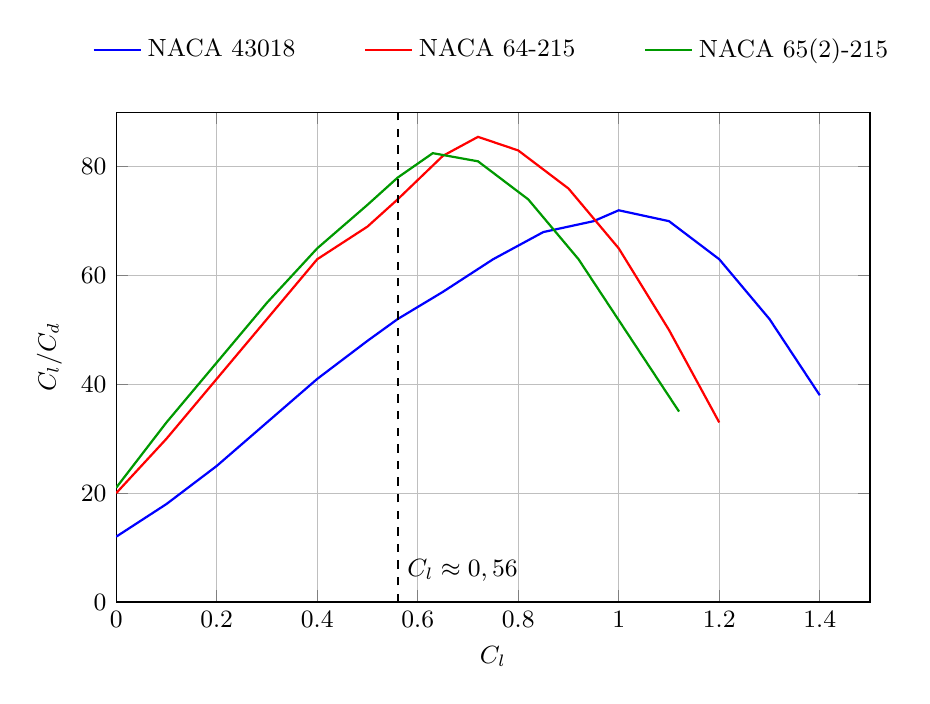
\begin{tikzpicture}
    \begin{axis}[
        width=0.92\linewidth,
        height=7.8cm,
        xlabel={$C_l$},
        ylabel={$C_l/C_d$},
        xmin=0, xmax=1.50,
        ymin=0, ymax=90,
        grid=major,
        tick label style={font=\small},
        label style={font=\small},
        every axis plot/.append style={thick},
        legend columns=3,
        legend style={
            at={(0.5,1.08)},
            anchor=south,
            font=\small,
            draw=none,
            fill=none,
            /tikz/every even column/.append style={column sep=0.8cm}
        }
    ]

    % NACA 43018
    \addplot[color=blue] coordinates {
        (0.00,12)
        (0.10,18)
        (0.20,25)
        (0.30,33)
        (0.40,41)
        (0.50,48)
        (0.56,52)
        (0.65,57)
        (0.75,63)
        (0.85,68)
        (0.95,70)
        (1.00,72)
        (1.10,70)
        (1.20,63)
        (1.30,52)
        (1.40,38)
    };
    \addlegendentry{NACA 43018}

    % NACA 64-215
    \addplot[color=red] coordinates {
        (0.00,20)
        (0.10,30)
        (0.20,41)
        (0.30,52)
        (0.40,63)
        (0.50,69)
        (0.56,74)
        (0.65,82)
        (0.72,85.5)
        (0.80,83)
        (0.90,76)
        (1.00,65)
        (1.10,50)
        (1.20,33)
    };
    \addlegendentry{NACA 64-215}

    % NACA 65(2)-215
    \addplot[color=green!60!black] coordinates {
        (0.00,21)
        (0.10,33)
        (0.20,44)
        (0.30,55)
        (0.40,65)
        (0.50,73)
        (0.56,78)
        (0.63,82.5)
        (0.72,81)
        (0.82,74)
        (0.92,63)
        (1.02,49)
        (1.12,35)
    };
    \addlegendentry{NACA 65(2)-215}

    % Condição de projeto
    \addplot[color=black, dashed] coordinates {(0.56,0) (0.56,90)};
    \node[anchor=south west, font=\small]
        at (axis cs:0.56,2) {$C_l \approx 0,56$};

    \end{axis}
    \end{tikzpicture}

    \caption{Eficiência aerodinâmica dos perfis avaliados.}
    \label{fig:comparacao_clcd_cl}
\end{figure}

Os perfis laminares da série NACA 6 apresentaram maior eficiência aerodinâmica na condição analisada. Entretanto, sua vantagem depende da manutenção de uma superfície limpa e com baixa rugosidade, condição que pode ser comprometida por contaminação, chuva, insetos e formação de gelo. Por esse motivo, nesta etapa do projeto não foi adotado um perfil laminar como requisito, mantendo-se a família NACA 430XX como referência por apresentar maior robustez operacional.

Também é prevista a utilização de um sistema de proteção contra gelo nos bordos de ataque da asa e das empenagens, com a solução de degelo ou antigelo a ser definida em etapas posteriores do projeto. Essa previsão deve ser considerada na geometria e no acabamento superficial do bordo de ataque, especialmente por sua influência sobre a transição da camada limite e, consequentemente, sobre os benefícios associados ao escoamento laminar.

Definida a família do perfil, a seção seguinte determina a espessura relativa necessária ao longo da semi-envergadura a partir dos requisitos estruturais da asa.


\subsection{Análise da Espessura Relativa} 
\label{analise_espessura}

Para estimar os esforços na asa, adotou-se o método de Stender, no qual a sustentação local é proporcional a uma corda equivalente dada pela média geométrica entre as cordas trapezoidal e elíptica.

Utilizando as dimensões de asa previamente definidas: $b = 28,5$ m, $\lambda = 0,405$, AR = 10,96 e $S = 74,1$ $m^2$; e considerando a condição crítica de MTOW com um fator de carga igual a 2,5, a distribuição de sustentação ao longo da semi-envergadura da asa da aeronave é apresentada na Figura \ref{fig:distribuição de sustentação}.

\begin{figure} [H]
    \centering
    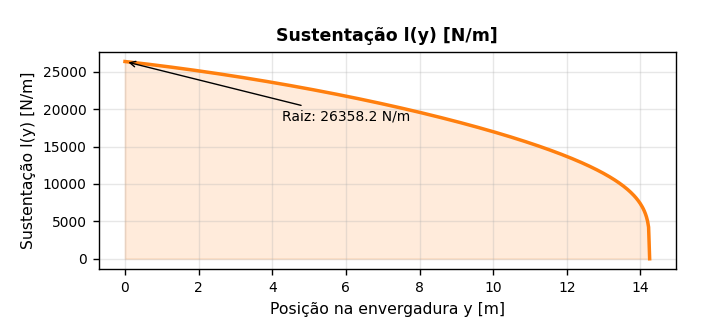
\includegraphics[width=0.7\linewidth]{images/Distribuição de Sustentação.png}
    \caption{Distribuição de sustentação ao longo da semi-envergadura.}
    \label{fig:distribuição de sustentação}
\end{figure}

Vale pontuar que, para a obtenção dessa distribuição por meio do método de Stender, foi feita uma discretização da semi-asa em 500 pontos. 

A partir da distribuição de sustentação, a força cortante e o momento fletor foram obtidos por integração numérica pelo método do trapézio:

\begin{equation}
    V(y) = \int_{0}^{\frac{b}{2}} L(y) \, dy
    \label{cortante}
\end{equation}

\begin{equation}
    M(y) = \int_{0}^{\frac{b}{2}} V(y) \, dy
    \label{momento fletor}
\end{equation}

\begin{figure} [H]
    \centering
    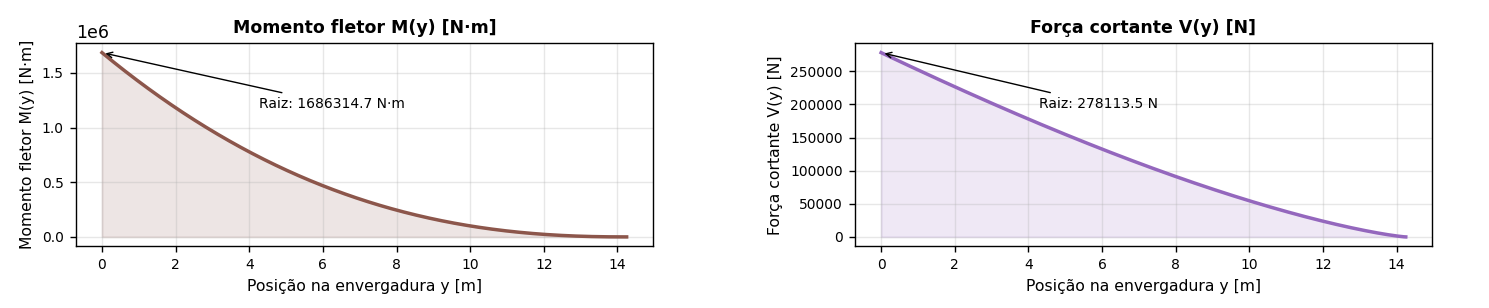
\includegraphics[width=1.0\linewidth]{images/Cortantes e Momentos na Asa.png}
    \caption{Momento fletor e força cortante ao longo da semi-envergadura.}
    \label{fig:Momentos e Cortantes na Asa}
\end{figure}

Para estimar a espessura mínima do perfil, considerou-se uma longarina equivalente de seção I, cuja altura $h$ é limitada pelos esforços locais. Foram adotadas mesas com espessura de $5\%h$ e largura de $25\%h$, e alma com espessura de $10\%h$. As tensões foram avaliadas no bordo da mesa, na junção mesa-alma e na linha neutra, por:

\begin{equation}
    \sigma=\frac{M \cdot z}{I}
    \label{tensão normal}
\end{equation}

\begin{equation}
    \tau = \frac{V \cdot Q}{I \cdot t}
    \label{tensão cisalhante}
\end{equation}

onde t é a espessura da chapa do ponto analisado.

A tensão equivalente de Von Mises foi comparada ao limite de escoamento do alumínio 7075-T6, adotado como $\sigma_y=480$ MPa:

\begin{equation}
    \sigma_{eq} = \sqrt{\sigma^2+3\tau^2}
    \label{tensão equivalente}
\end{equation}

Como a altura $h$ da longarina limita a espessura do perfil, adotou-se $t/c=h/c$ para avaliar a espessura relativa mínima ao longo da semi-envergadura. Foram analisados valores entre 9\% e 21\%, conforme a Figura \ref{fig:tensão de von mises}.

\begin{figure} [H]
    \centering
    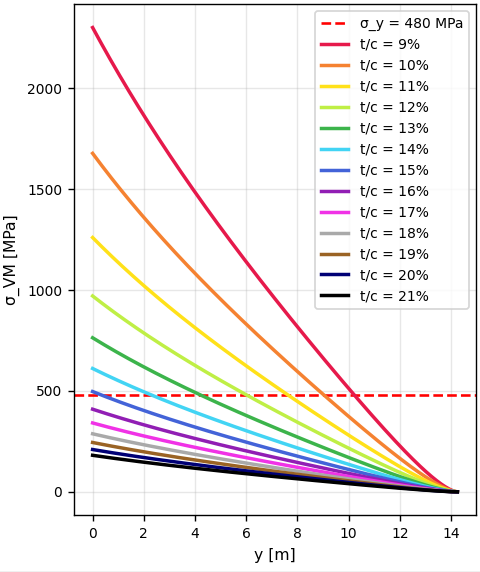
\includegraphics[width=0.5\linewidth]{images/Tensão de Von Mises.png}
    \caption{Tensão de Von Mises ao longo da semi-envergadura para diferentes espessuras relativas.}
    \label{fig:tensão de von mises}
\end{figure}

Na raiz, valores de $t/c \leq 15\%$ levam ao escoamento, enquanto na ponta todos os valores avaliados atendem ao critério estrutural. Visando reduzir o arrasto parasita, adotou-se o menor valor que atende ao critério em cada região: $t/c=16\%$ na raiz e $t/c=9\%$ na ponta, com transição linear entre ambos. A Figura \ref{fig:transição linear de perfil} confirma que a transição linear adotada permanece acima da espessura estrutural mínima ao longo de toda a semi-envergadura.

\begin{figure} [H]
    \centering
    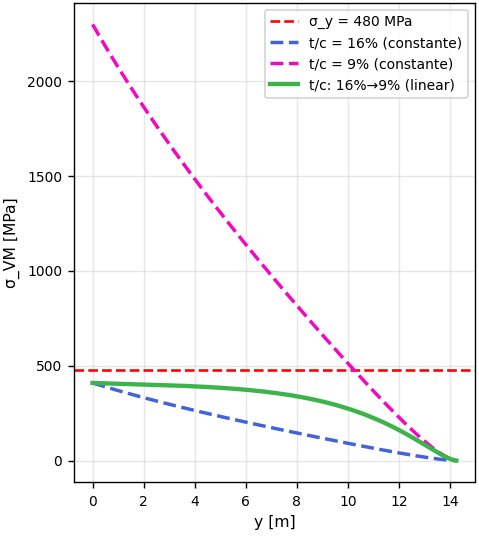
\includegraphics[width=0.5\linewidth]{images/Transição linear do perfil.png}
    \caption{Avaliação da transição linear dos perfis ao longo da semi-envergadura.}
    \label{fig:transição linear de perfil}
\end{figure}

\subsection{Definição Final do Perfil}
\label{subsec:definiçãoPerfil}

Portanto, reunindo todas as informações das últimas seções, os perfis definidos para a asa do projeto são:

\begin{itemize}
    \item Raiz da Asa: NACA 43016
    \item Ponta da Asa: NACA 43009
\end{itemize}

Eles são mostrados sobrepostos na Figura \ref{fig:PerfisDaAsa}.

\begin{figure} [H]
    \centering
    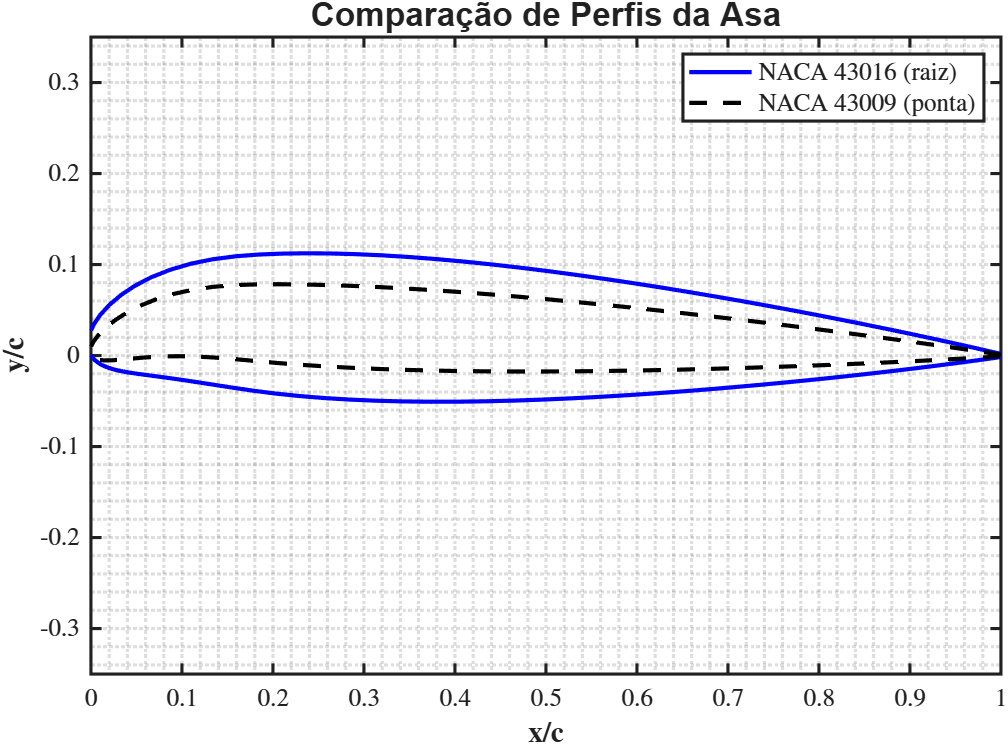
\includegraphics[width=0.6\linewidth]{images/PerfisDaAsa.png}
    \caption{Perfis da raiz e ponta de asa}
    \label{fig:PerfisDaAsa}
\end{figure}

\subsection{Análise Tridimensional da Asa no XFLR5}

A fim de verificar as curvas aerodinâmicas da asa, os valores da Tabela \ref{tab:dimensoes_conclusao} e os dados obtidos por análise no XFLR5 dos perfis obtidos na seção \ref{subsec:definiçãoPerfil} foram importados para a seção de desenho 3D no software mencionado.

\begin{figure}[H]
    \centering
    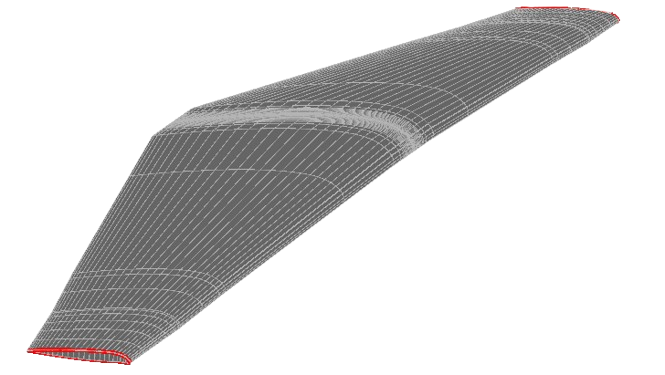
\includegraphics[width=0.8\linewidth]{images/AsaXFLR5.png}
    \caption{Asa desenhada no XFLR5}
    \label{fig:AsaXFLR5}
\end{figure}

Com isso, para a velocidade de cruzeiro $V_c = 260 \text{ kt} \approx 134 \text{ m/s}$, as seguintes curvas foram obtidas (Figuras \ref{fig:polar_arrasto} e \ref{fig:eficiencia_aero}):

\begin{figure}[H]
    \centering
    \begin{minipage}{0.48\textwidth}
        \centering
        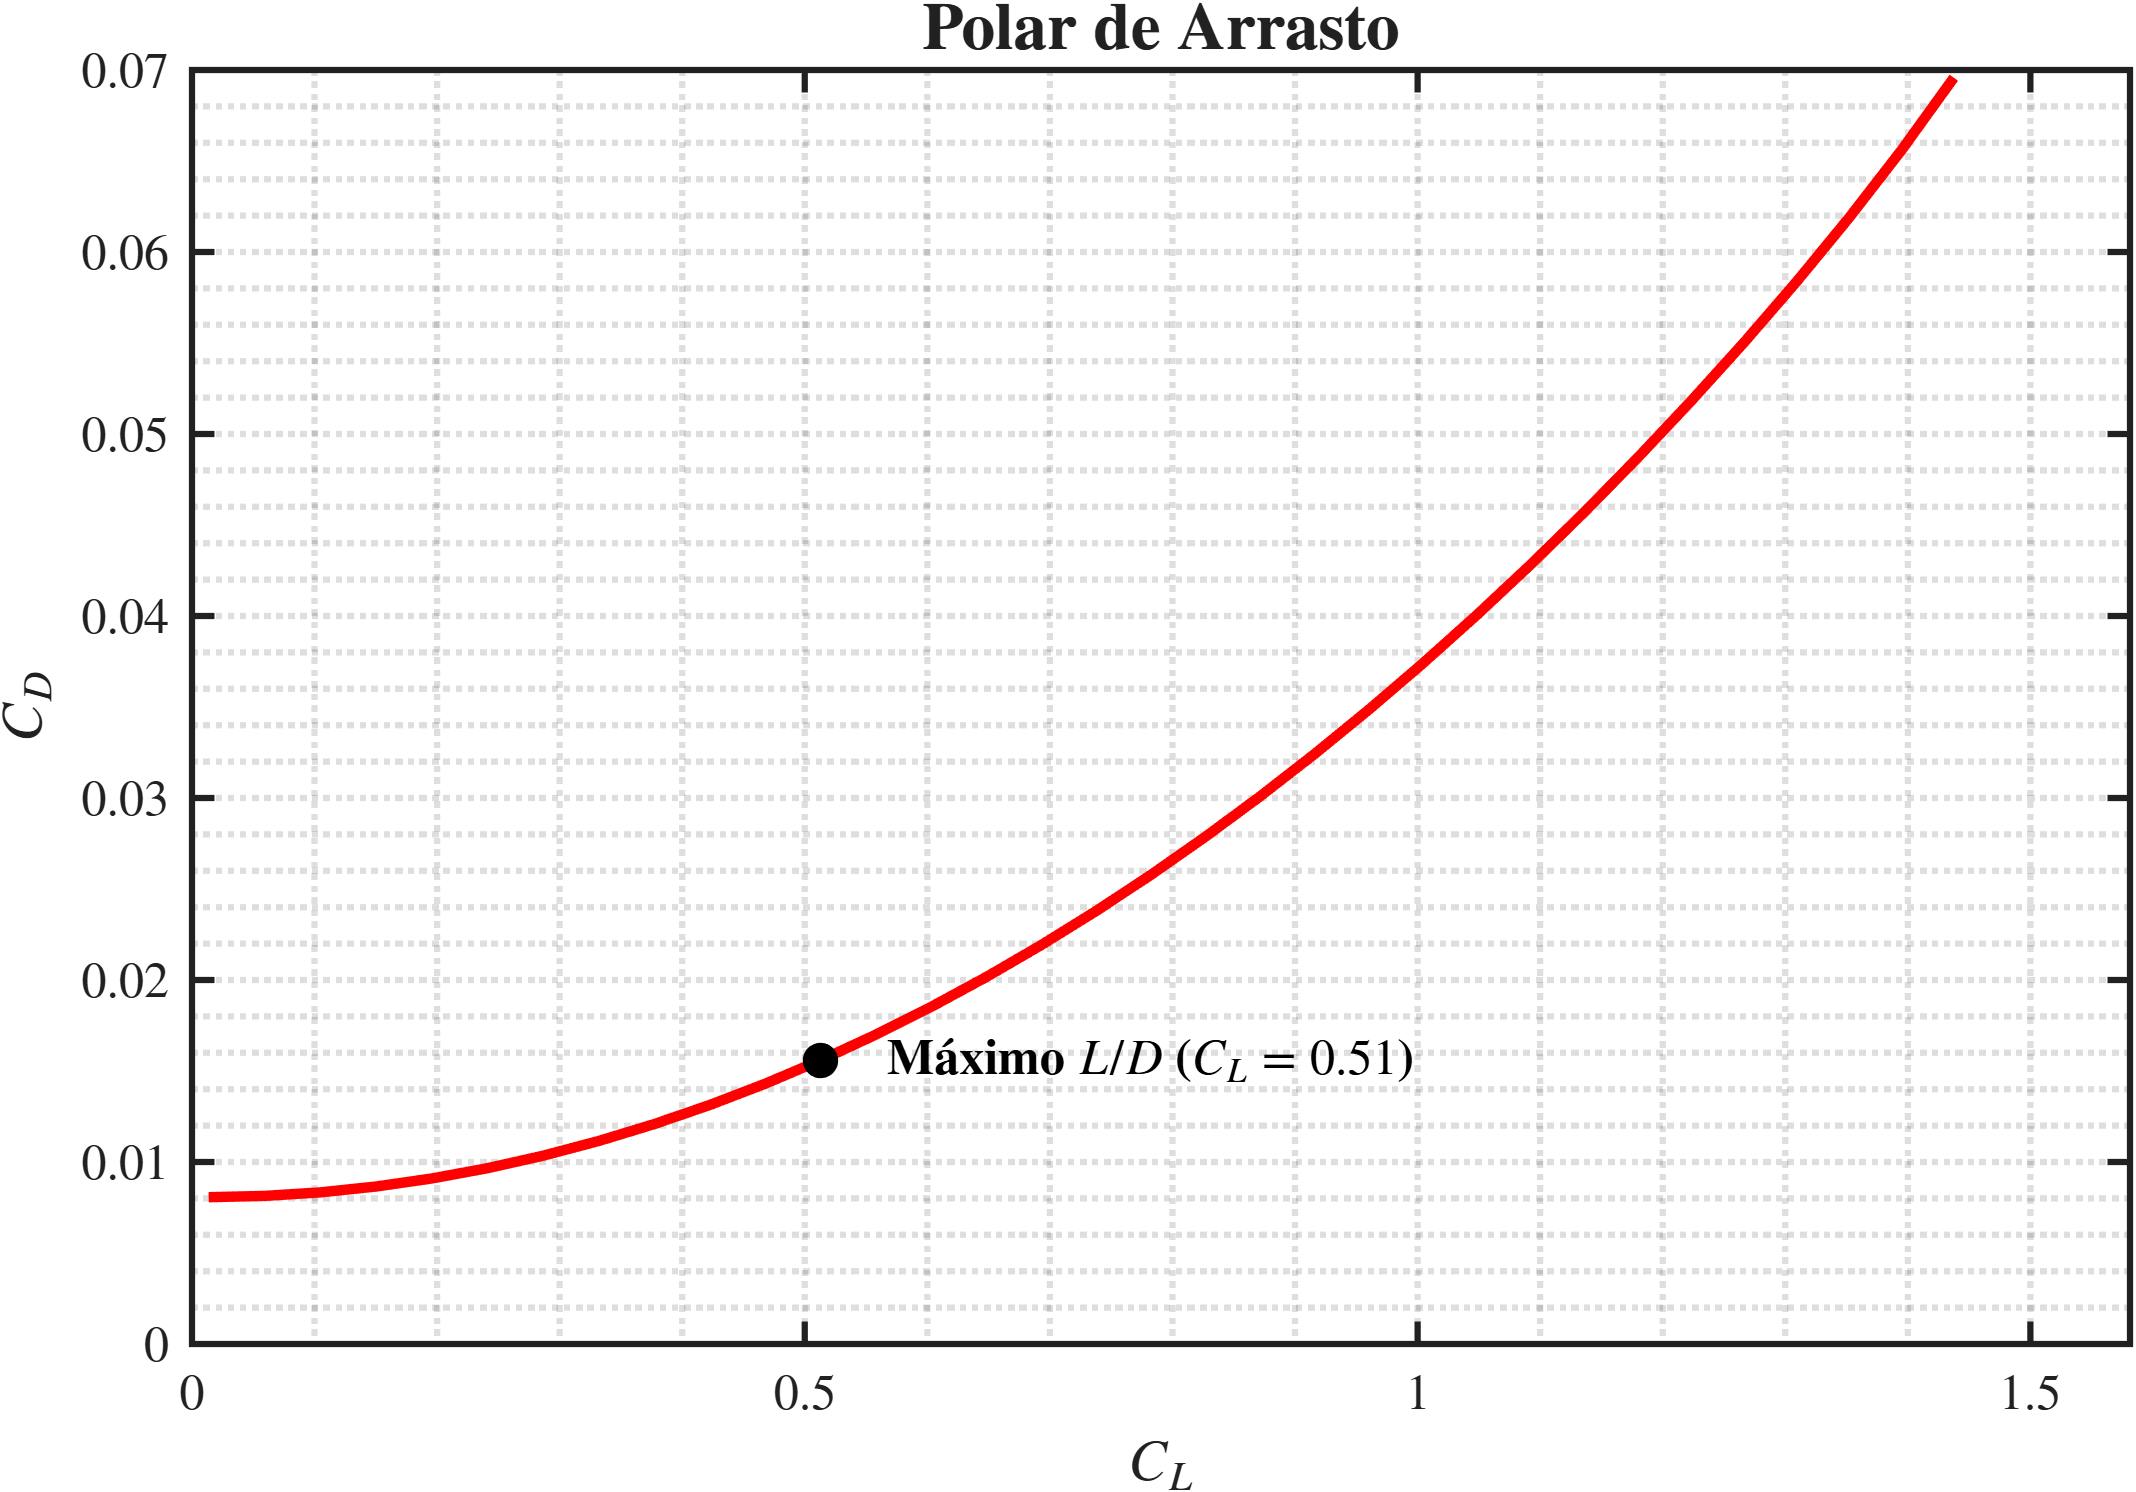
\includegraphics[width=\linewidth]{images/Polar_Arrasto_CL_CD.png}
        \caption{Polar de arrasto da asa ($C_D \times C_L$).}
        \label{fig:polar_arrasto}
    \end{minipage}\hfill
    \begin{minipage}{0.48\textwidth}
        \centering
        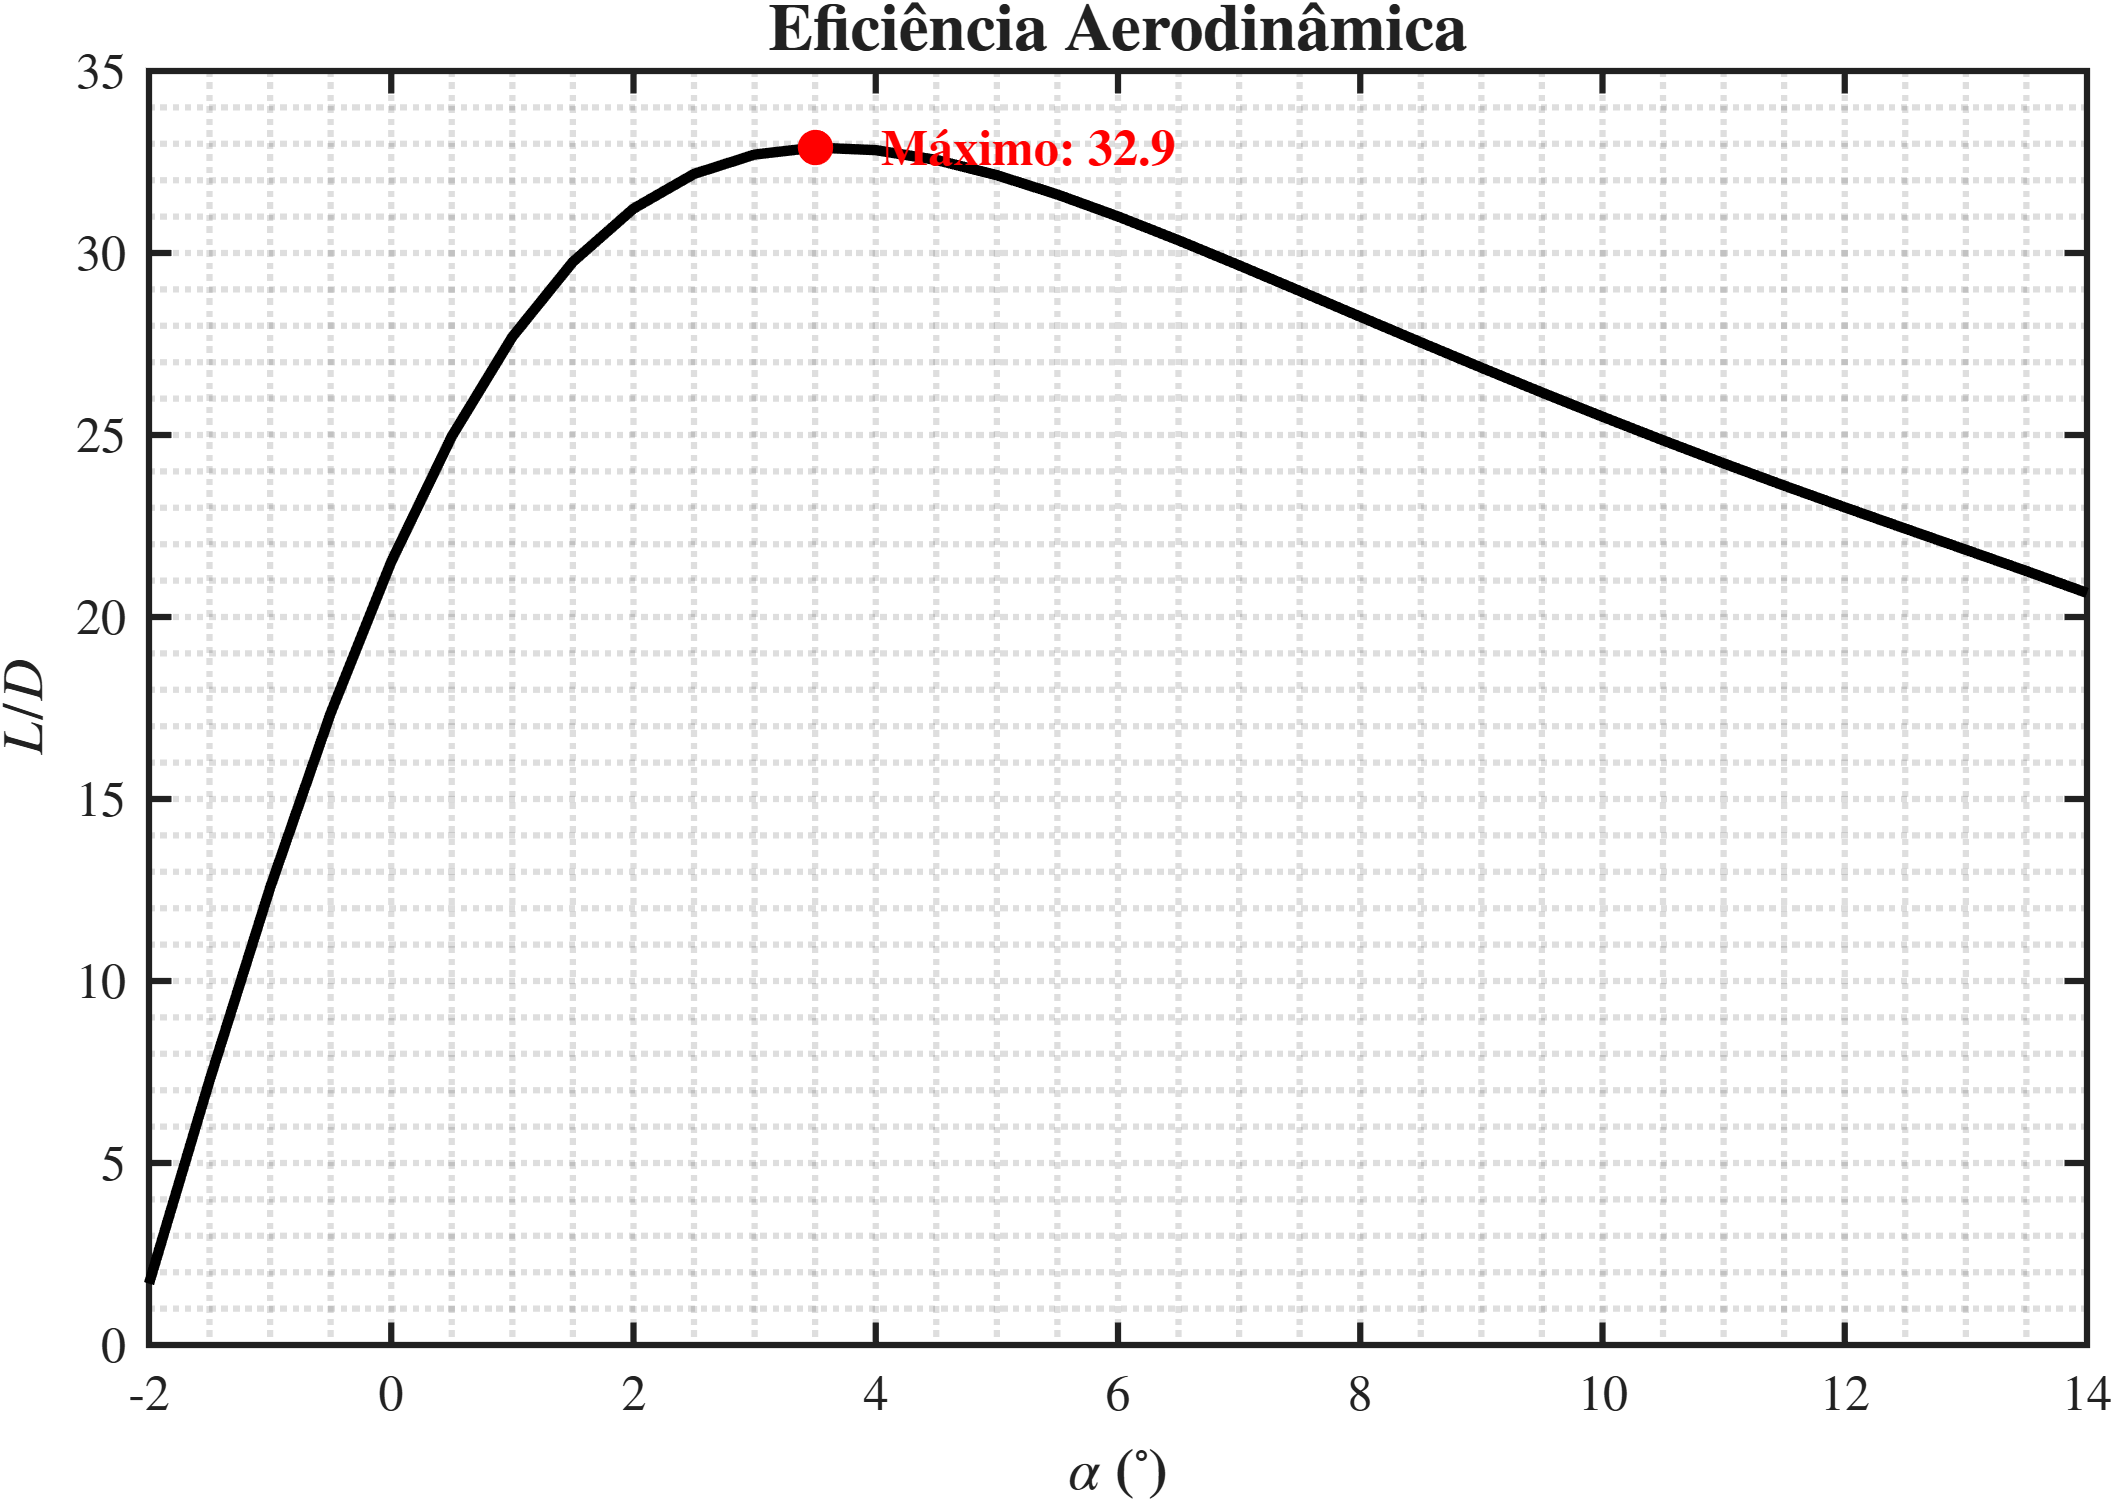
\includegraphics[width=\linewidth]{images/Eficiencia_Aerodinamica.png}
        \caption{Curva de eficiência aerodinâmica ($L/D \times \alpha$).}
        \label{fig:eficiencia_aero}
    \end{minipage}
\end{figure}

A eficiência máxima foi $L/D \approx 32,9$ em $C_L=0,51$, valor próximo ao coeficiente de sustentação de projeto e compatível com a condição de cruzeiro adotada.


\subsection{Dimensionamento dos Flaps}

A determinação do coeficiente de sustentação máximo na configuração limpa,
$C_{L_{\max,\text{limpo}}}$, constitui o ponto de partida para o dimensionamento
do sistema de hipersustentação. Este valor foi obtido por meio de simulação
numérica no software XFLR5, apresentado anteriormente. O resultado desta análise
é apresentado na Figura~\ref{fig:xflr5CLmax}, da qual extrai-se:
 
\begin{equation}
    C_{L_{\max,\text{limpo}}} \approx 1{,}50
\end{equation}
 
\begin{figure}[H]
    \centering
    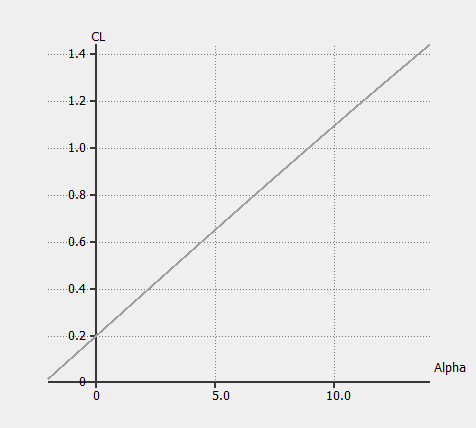
\includegraphics[width=0.50\linewidth]{images/xflr5CLmax.png}
    \caption{Gráfico $C_L$ por $\alpha$ obtido no XFLR5.}
    \label{fig:xflr5CLmax}
\end{figure}

\begin{equation}
\label{eq:CLnormal}
    C_L = \frac{MTOW \cdot g}{\frac{1}{2}\rho V^2 S_{wing}}
\end{equation}

A partir da equação \ref{eq:CLnormal}, adaptada para isolar a velocidade,
conforme a equação \ref{eq:Vestol}:

\begin{equation}
    V_{\text{estol}} = \sqrt{\frac{2W}{\rho\, C_{L_{\max}}\, S}}
    \label{eq:Vestol}
\end{equation}

\noindent encontra-se a velocidade de estol na configuração limpa,
$V_{\text{estol,limpo}} = 111$~kt, correspondente ao $C_{L_{\max,\text{limpo}}} = 1{,}50$
obtido numericamente no XFLR5.

Por meio das análises comparativas com as aeronaves similares apresentadas na
Tabela~\ref{tab:perfiscomparativos}, estabeleceu-se que a velocidade máxima de
estol na configuração com flap é $V_{\text{estol,flap}} = 83$~kt. Aplicando
esta velocidade na equação \ref{eq:CLnormal}, determina-se o coeficiente de
sustentação máximo requerido na configuração com flap:

\begin{equation}
    C_{L_{\max,\text{flap}}} = 2{,}69
    \label{eq:CLmaxflap}
\end{equation}

As velocidades de operação para as fases de decolagem e pouso são definidas
pelo \S~25.107 e \S~25.125 do FAR Part~25~\cite{far25}, que estabelecem
fatores mínimos sobre a velocidade de pouso e decolagem a partir das velocidades de estol do projeto. Para a decolagem, a velocidade de segurança deve satisfazer:

\begin{equation}
    V_{decolagem} \geq 1{,}13 \cdot V_{\text{estol,limpo}}
    \label{eq:vto}
\end{equation}

\noindent e para o pouso, a velocidade deve satisfazer:

\begin{equation}
    V_\text{pouso} \geq 1{,}30 \cdot V_{\text{estol,flaps}}
    \label{eq:vref}
\end{equation}

A partir das equações \ref{eq:CLnormal}, \ref{eq:vto} e \ref{eq:vref}, calculam-se
as velocidades operacionais e os respectivos coeficientes de sustentação, evidenciados na tabela a seguir.

\begin{table}[H]
    \centering
    \caption{Coeficientes de sustentação e velocidades por condição de voo.}
    \label{tab:clmax}
    \begin{tabular}{lcc}
        \toprule
        \textbf{Condição} & \textbf{Velocidade (kt)} & $\boldsymbol{C_L}$ \\
        \midrule
        Estol limpo  (XFLR5)                                       & 111 & 1,50 \\
        Decolagem ($1{,}13\,V_{\text{estol,limpo}}$, \S~25.107) & 125 & 1,17 \\
        Estol com flap (análise comparativa)                 &  83 & 2,69 \\
        Pouso ($1{,}30\,V_{\text{estol,flap}}$, \S~25.125)  & 108 & 1,59 \\
        \bottomrule
    \end{tabular}
\end{table}

\noindent A partir dos valores consolidados na Tabela~\ref{tab:clmax}, verifica-se que
os $C_L$ operacionais de decolagem e pouso se situam no máximo até
 $C_{L_{\max,\text{flap}}} = 2{,}69$,
o que garante a viabilidade do projeto do sistema de hipersustentação. 

Com todos os valores de $C_L$ importantes do projeto explicitados, calcula-se
o incremento de sustentação necessário $\Delta C_{L_{\max}}$ entre a
configuração limpa e a configuração com flap:

\begin{equation}
    \Delta C_{L_{\max}} = C_{L_{\max,\text{flap}}} - C_{L_{\max,\text{limpo}}}
    = 2{,}69 - 1{,}50 = 1{,}19
    \label{eq:deltaCL}
\end{equation}

\noindent Este valor orienta a escolha do tipo de flap mais adequado ao projeto,
uma vez que diferentes dispositivos de hipersustentação produzem incrementos
distintos de $C_{L_{\max}}$. 

Com base na Tabela~12.2 do capítulo 12.4.6 de \cite{raymer2018}, que apresenta
os incrementos típicos de $C_{L_{\max}}$ para diferentes dispositivos de
hipersustentação, optou-se pelo flap \textit{single slotted}, o qual oferece
um incremento máximo de $\Delta C_{L_{\max}} = 1{,}3$. Este valor supera o
incremento requerido pelo projeto de $\Delta C_{L_{\max}} = 1{,}19$,
confirmando que o dispositivo escolhido é capaz de atender aos requisitos
estabelecidos pelo \S~25.107 e \S~25.125 do FAR Part~25~\cite{far25}.

Os ângulos de deflexão adotados para o sistema de flap são de $10^{\circ}$ para a
decolagem e $40^{\circ}$ para o pouso. Estas configurações foram simuladas no XFLR5
utilizando \textit{plain flaps}, uma vez que o simulador não dispõe de modelos
para o flap \textit{single slotted} escolhido. Por ser um dispositivo de menor
eficiência aerodinâmica que o \textit{single slotted}, o \textit{plain flap}
representa apenas uma visualização do incremento de sustentação em operação que deve ser superada.


\begin{figure} [h]
    \centering
    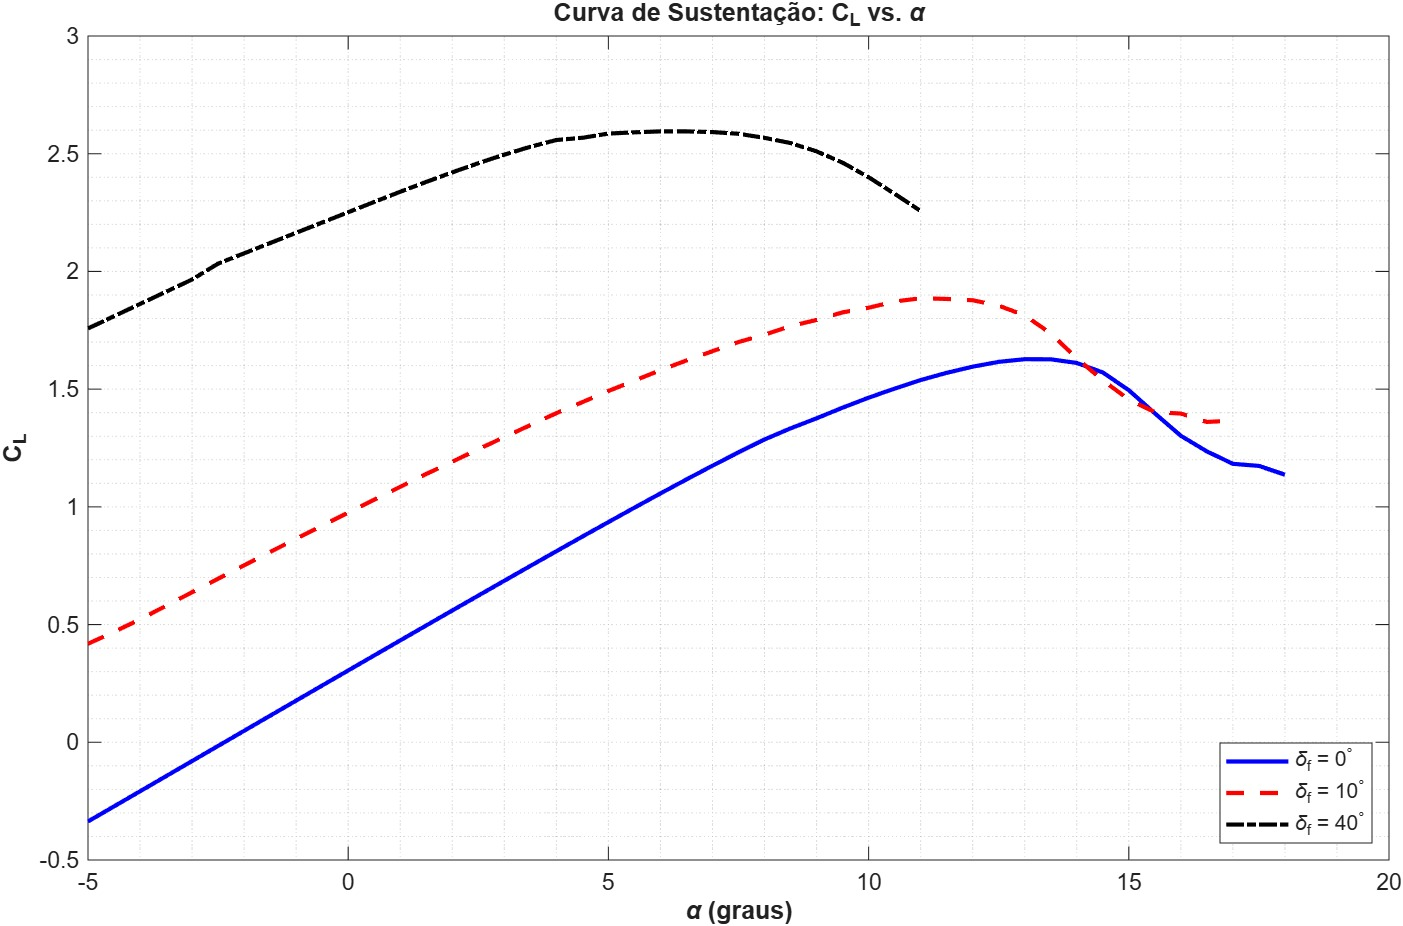
\includegraphics[width=0.8\linewidth]{falpslegais.png}
    \caption{Efeito dos flaps simulados}
    \label{fig:efeito dos flaps}
\end{figure}

\subsection{\textit{Washout}}

Com a forma em planta e os perfis aerodinâmicos previamente definidos, procedeu-se à avaliação da implementação de torção geométrica negativa (\textit{washout}) nas pontas da asa. Esta modificação teve como objetivos principais o incremento da eficiência aerodinâmica global da aeronave, visando otimizar o alcance e minimizar os custos operacionais e o consumo de energia em rota, a atenuação da intensidade dos vórtices de ponta e a redução do momento fletor na raiz por meio da redistribuição do carregamento ao longo da envergadura. Ademais, o \textit{washout} foi projetado para garantir características favoráveis e seguras de estol, induzindo o deslocamento do início do estol para a região entre $33\%b$ e $40\%b$ da semi-envergadura, preservando assim a autoridade de rolamento nas fases críticas de voo \cite{raymer1992}.

\begin{figure}[H]
    \centering
    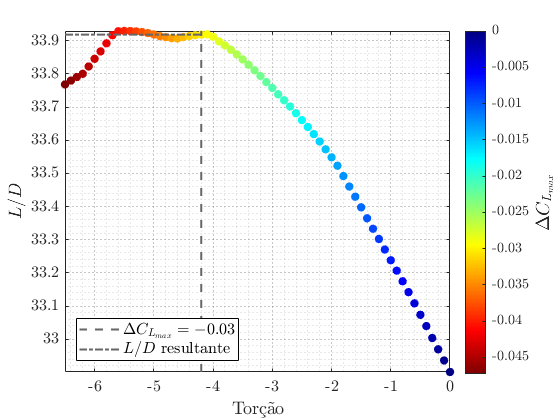
\includegraphics[width=0.7\linewidth]{images/washout_LD.png}
    \caption{Sensibilidade de $\frac{L}{D}$}
    \label{fig:wahsout_LD}
\end{figure}

\begin{figure}[H]
    \centering
    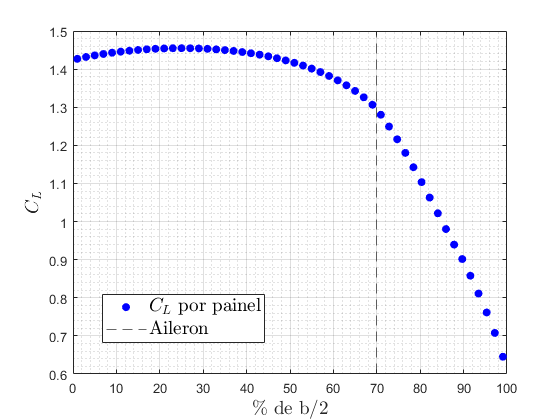
\includegraphics[width=0.7\linewidth]{images/washout_estol.png}
    \caption{Distribuição de $C_L$ por painel}
    \label{fig:washout_estol}
\end{figure}

Como observado na \autoref{fig:wahsout_LD}, a adoção de ângulos de torção muito acentuados acarreta uma degradação geométrica que penaliza o coeficiente de sustentação máximo da asa. Dessa forma, buscando o melhor balanço entre o $L/D$ e $C_{L_{max}}$, adotou-se a maior torção admissível tal que a penalidade no limite de sustentação fosse restrita a $\Delta C_{L_{max}} \geq -0.03$, possibilitanto o ganho de $\Delta \frac{L}{D}_{max} \approx1$.

\section{Geometria das Empenagens e Superficies de Controle}

\subsection{Empenagens Horizontal e Vertical}

O valor dos volumes de cauda definidos no anteprojeto se mantiveram onde: 

\begin{equation*}
    \overline{V}_{HT} = 1,1   \qquad  \overline{V}_{VT} = 0,08
\end{equation*}

A partir dos volumes de cauda e dos valores já definidos de geometria da asa, assim como por meio de análises comparativas já mostradas anteriormente, foram definidas as geometrias das empenagens horizontal e vertical.




\begin{table}[H]
    \centering
    \caption{Geometria da empenagem horizontal}
    \begin{tabular}{c c c c c c c}
    \hline
     $S_{HT}$  & $b_{HT}$ & $c_{r_{HT}}$ & $l_{EH}$ & $\lambda_{HT}$ & $\Gamma_{HT}$ & $\Lambda_{HT}$ \\
     \hline
     18,679 m$^2$ & 8,375 m & 2,788 m & 12,0 m & 0,60 & 0 $\degree$ &  8,5$\degree$ \\
     \hline
    \end{tabular}
    \label{GeoEH_Final}
\end{table}

\begin{table}[H]
    \centering
    \caption{Geometria da empenagem vertical.}
    \begin{tabular}{c c c c c c c}
    \hline
     $S_{VT}$  & $b_{VT}$ & $c_{r_{VT}}$ & $l_{VH}$ & $\lambda_{VT}$ & $\Gamma_{VT}$ & $\Lambda_{VT}$ \\
     \hline
     15,359 m$^2$ & 4,925 m & 4,158 m & 11,0 m & 0,50 & 0 $\degree$ &  25$\degree$ \\
     \hline
    \end{tabular}
    \label{GeoEV_Final}
\end{table}

Para a definição do perfil das empenagens foi realizada a mesma análise de momento e cortante feita na asa, na sessão \ref{analise_espessura}. A força de sustentação da empenagem horizontal foi considerada como sendo a força de balanceamento para voo reto nivelado ao nível do mar. Dessa forma, foi escolhido o perfil simétrico NACA 0012.

\subsection{Superfícies de Controle}

Para o dimensionamento das superfícies de controle, foram novamente utilizados os dados da análise comparativa.

\subsubsection{Profundor}

Para o profundor foi decido que sua corda é constante, com valor igual a 30\% da corda na raiz ($c_r$) do estabilizador horizontal, e cobrindo toda sua envergadura.


\begin{table}[H]
    \centering
     \caption{Dimensões do profundor.}
    \begin{tabular}{c c c}
    \hline
     $S_{\eta}$  & $\overline{c_{\eta}}$ & $b_{\eta}$  \\
     \hline
     5,721 m$^2$ & 0,683 m & 8,375 m \\
      \hline
    \end{tabular}
    \label{Profundor_geo}
\end{table}


\subsubsection{Leme}

Para o leme foi definido que sua corda será constante com valor de 30\% da corda na raiz da empenagem vertical, e também ocupa toda sua envergadura.

\begin{table}[H]
    \centering
     \caption{Dimensões do leme.}
    \begin{tabular}{c c c}
    \hline
     $S_{\zeta}$  & $\overline{c_{\zeta}}$ & $b_{\zeta}$  \\
     \hline
     4,778 m$^2$ & 0,97 m & 4,925 m \\
      \hline
    \end{tabular}
    \label{leme_geo}
\end{table}


\subsubsection{Aileron}

Os ailerons possuem corda constante ao equivalente de 30\% da corda média aerodinâmica, e possuem uma envergadura de 25\% da envergadura da aeronave. Sua posição está mais afastada das asas, a uma distância de 70\% da metade de sua envergadura. As dimensões apresentadas na tabela a seguir já englobam ambos os ailerons direito e esquerdo.

\begin{table}[H]
    \centering
     \caption{Dimensões dos ailerons.}
    \begin{tabular}{c c c}
    \hline
     $S_{\xi}$  & $\overline{c_{\xi}}$ & $b_{\xi}$  \\
     \hline
     5,878 m$^2$ & 0,825 m & 3,563 m \\
      \hline
    \end{tabular}
    \label{ailer_geo}
\end{table}


\section{Geometria interna}

\subsection{Ergonomia}
\label{sec:ergonomia}

O desenvolvimento da cabine de comando foi realizado com base nos requisitos
estabelecidos pela regulamentação de aviação 14 CFR Part 25
(\S 25.771 a \S 25.781), que trata dos aspectos relacionados ao cockpit e à
interação do piloto com os comandos. O requisito 14 CFR Part 25
(\S 25.771) estabelece que a cabine deve permitir operação segura e eficiente
da aeronave, garantindo adequada disposição dos tripulantes e dos comandos.
Já 14 CFR Part 25 (\S 25.773) define requisitos relacionados ao campo de visão
do piloto, exigindo visibilidade adequada durante táxi, decolagem e pouso.
Os requisitos 14 CFR Part 25 (\S 25.777 e \S 25.779) abordam a disposição,
acessibilidade e movimentação dos controles, visando reduzir a possibilidade
de erros operacionais, enquanto 14 CFR Part 25 (\S 25.781) estabelece critérios
para diferenciação tátil e visual das manetes e comandos principais.

Entretanto, a 14 CFR Part 25 apresenta esses requisitos de maneira
predominantemente qualitativa, sem especificar dimensões geométricas fixas
para o dimensionamento da cabine de comando. Dessa forma, para o
desenvolvimento dos desenhos deste projeto, utilizou-se como referência a
aeronave ATR 72-600, por possuir características operacionais e configuração
semelhantes às da aeronave desenvolvida neste trabalho. Em complemento à
geometria do ATR, para garantir o rigor do estudo ergonômico na modelagem no
Fusion 360, foram utilizadas as diretrizes do Human Factors Design Standard
(HFDS) da FAA. Desse documento, extraíram-se principalmente as dimensões
anatômicas estatísticas de pilotos dos sexos masculino e feminino em diferentes
percentis populacionais. A integração dessas duas referências norteou o
posicionamento relativo dos pilotos, a definição da geometria geral do cockpit
e a disposição dos painéis frontal, superior e pedestal central, além da
organização dos comandos de voo, navegação e gerenciamento dos motores.
Dessa maneira, os critérios ergonômicos relacionados ao alcance físico dos
controles, campo de visão do piloto, posicionamento dos displays principais e
separação funcional dos sistemas puderam ser quantificados, buscando atender
plenamente aos requisitos de operação segura, acessibilidade e visibilidade
previstos pela 14 CFR Part 25.

\begin{figure}[H]
    \centering
    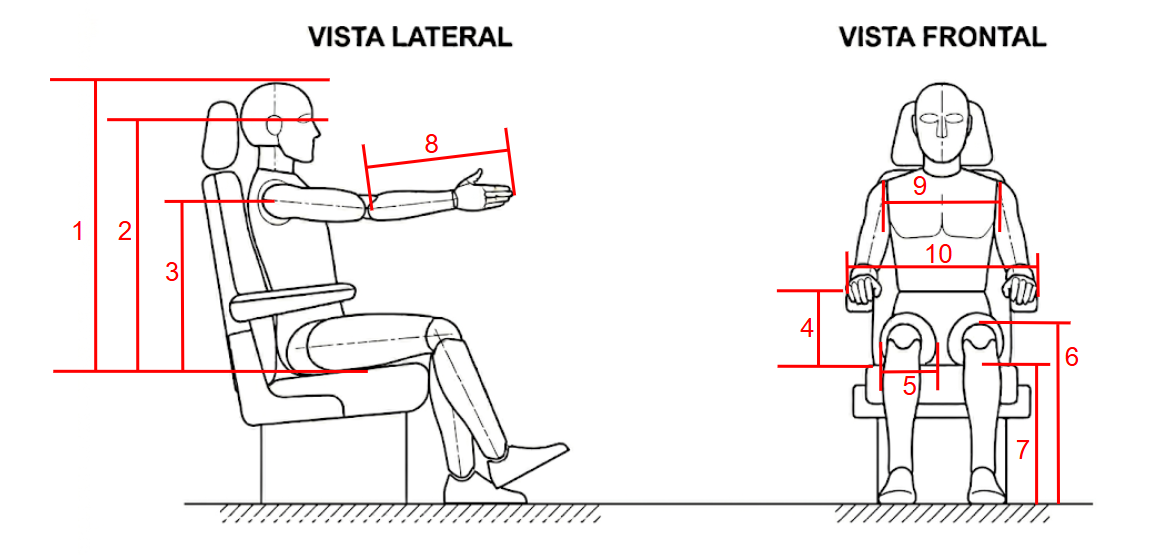
\includegraphics[width=0.60\textwidth]{images/Figura_3_27.png}
    \caption{Esquema de referência para as dimensões ergonômicas da cabine.}
    \label{fig:dimensoes_ergonomicas_cabine}
\end{figure}

\begin{table}[H]
\centering
\caption{Dimensões anatômicas estáticas detalhadas para ergonomia da cabine [cm].}
\label{tab:dimensoes_anatomicas_cabine}
\resizebox{\textwidth}{!}{%
\begin{tabular}{lcccccc}
\hline
\textbf{Dimensão} &
\multicolumn{3}{c}{\textbf{Masculino (M)}} &
\multicolumn{3}{c}{\textbf{Feminino (F)}} \\
\cline{2-7}
& \textbf{5º} & \textbf{50º} & \textbf{95º}
& \textbf{5º} & \textbf{50º} & \textbf{95º} \\
\hline
1 - Altura em posição sentada &
85,8 & 91,4 & 97,2 & 79,5 & 85,1 & 91,0 \\

2 - Altura dos olhos, sentado &
73,5 & 79,2 & 84,8 & 68,5 & 73,8 & 79,4 \\

3 - Altura do ombro, sentado &
54,9 & 59,8 & 64,6 & 50,9 & 55,5 & 60,4 \\

4 - Altura do cotovelo, sentado &
18,4 & 23,2 & 27,4 & 17,6 & 22,1 & 26,4 \\

5 - Espessura da coxa &
14,9 & 16,8 & 19,0 & 14,0 & 15,8 & 18,0 \\

6 - Altura do joelho, sentado &
51,4 & 55,8 & 60,6 & 47,4 & 49,8 & 56,0 \\

7 - Altura poplítea, sentado &
39,5 & 43,3 & 47,6 & 35,1 & 38,9 & 42,9 \\

8 - Comprimento antebraço-ponta do dedo &
44,8 & 48,3 & 52,4 & 40,6 & 44,2 & 48,3 \\

Alcance funcional do braço &
73,9 & 80,0 & 86,7 & 67,7 & 73,4 & 79,7 \\

9 - Largura dos ombros (bideltoide) &
45,0 & 49,1 & 53,5 & 39,7 & 43,1 & 47,2 \\

10 - Largura entre cotovelos &
47,8 & 54,5 & 62,1 & 41,5 & 46,7 & 52,8 \\
\hline
\end{tabular}%
}

\vspace{0.2cm}
\small Fonte: Adaptado de FAA HFDS, Seção 5.12.3.2.
\end{table}

Com base no levantamento das dimensões anatômicas detalhadas e nos requisitos
operacionais preestabelecidos, desenvolveu-se um modelo tridimensional
preliminar da cabine de comando utilizando o software Fusion 360. As figuras
a seguir apresentam os esboços iniciais resultantes dessa modelagem. Por se
tratar de uma concepção conceitual, a geometria e o arranjo apresentados estão
sujeitos a refinamentos e possíveis alterações nas fases subsequentes do projeto.
Contudo, esses modelos já fornecem uma visualização consistente da disposição
espacial interna, elaborada com foco contínuo na ergonomia da tripulação.
O dimensionamento físico das estações de trabalho foi conduzido com o objetivo
de garantir a correta acomodação dos pilotos, assegurando a acessibilidade física
aos comandos e a estrita manutenção dos volumes de tolerância, de modo a evitar
colisões ou restrições de espaço entre os ocupantes e a estrutura da cabine de
piloto. O resultado está apresentado nas imagens a seguir:

\begin{figure}[H]
    \centering
    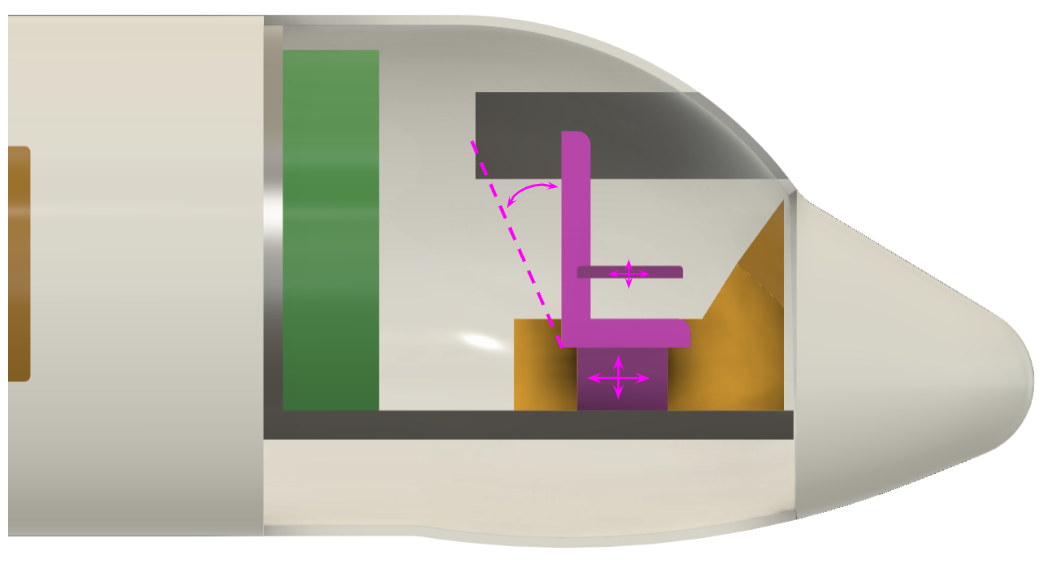
\includegraphics[width=0.70\textwidth]{images/Figura_3_28.png}
    \caption{Visão geral do arranjo ergonômico preliminar da cabine de comando.}
    \label{fig:arranjo_ergonomico_cabine}
\end{figure}

\begin{figure}[H]
    \centering
    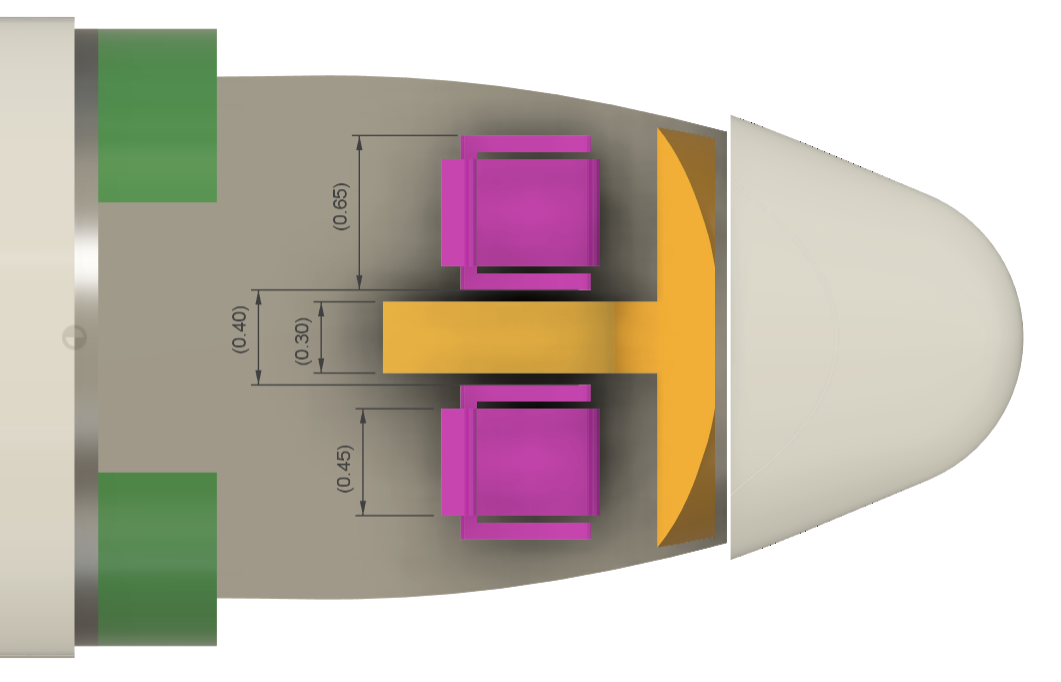
\includegraphics[width=0.70\textwidth]{images/Figura_3_29.png}
    \caption{Vista superior da disposição espacial.}
    \label{fig:vista_superior_cabine}
\end{figure}

\begin{figure}[H]
    \centering
    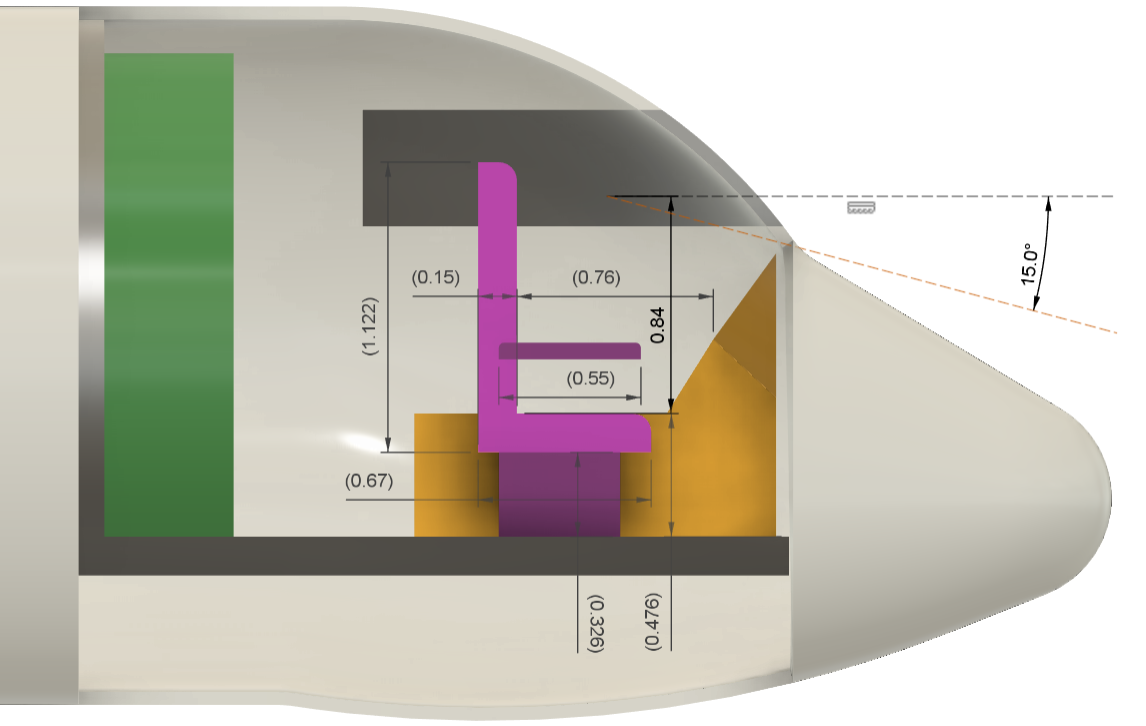
\includegraphics[width=0.70\textwidth]{images/Figura_3_30.png}
    \caption{Vista lateral do assento da tripulação de comando.}
    \label{fig:vista_lateral_assento}
\end{figure}

\subsection{Painel de Comando e Aviônicos}
\label{sec:painel_comando_avionicos}

A aeronave é certificada sob RBAC~25~\cite{rbac25}, FAR Part~25~\cite{far25} e
CS-25~\cite{cs25}, incluindo os requisitos associados à disposição dos
instrumentos e comandos no painel. O requisito determinante para o
\textit{layout} é o CS/FAR-25.1321, que estabelece critérios para o agrupamento
e posicionamento dos instrumentos de voo em relação ao plano vertical da visão
frontal do piloto. A disposição das informações primárias segue o conceito
denominado \textit{basic T}, herdado da instrumentação eletromecânica clássica
e mantido nos \textit{glass cockpits} por meio da representação gráfica
equivalente no \textit{Primary Flight Display} (PFD)~\cite{cs25,skybrary_pfd}.

Dessa forma, adota-se uma configuração \textit{glass cockpit} integrada,
compatível com o estado da arte em aeronaves turboélice regionais e tendo como
referência a arquitetura empregada no ATR 72-600. A escolha em detrimento da
instrumentação eletromecânica permite concentrar as principais informações de
voo, navegação, motorização e sistemas em displays eletrônicos, reduzindo a
quantidade de instrumentos individuais e favorecendo a integração das
informações apresentadas aos pilotos.

A disposição do painel é definida de forma integrada aos critérios
antropométricos apresentados na seção anterior. Seu posicionamento considera a
posição dos olhos dos pilotos, a linha normal de visada, o alcance funcional dos
membros superiores e a necessidade de preservar a visibilidade externa da
cabine. Dessa forma, busca-se manter as informações essenciais à condução da
aeronave no campo primário de visão e garantir adequada acessibilidade aos
comandos.

Na cabine de comando, mais especificamente no painel, são disponibilizadas aos
pilotos informações necessárias à aeronavegabilidade por meio dos aviônicos,
``equipamentos eletrônicos ou de processamento de dados utilizados para
controle, comunicação e/ou navegação em aeronaves'', segundo definição da
ANAC.

A instrumentação e equipamentos mínimos necessários para operação da aeronave é
estabelecida por meio do regulamento brasileiro de aviação civil e depende da
categoria da aeronave e dos equipamentos instalados, a exemplo do motor
utilizado. Desse modo, o RBAC~25 Subparte F~\cite{rbac25} determina que para
motores turboélice os seguintes equipamentos são necessários:

\begin{itemize}
    \item Indicador de combustível individual para cada motor;
    \item Alarmes de falhas/avisos;
    \item Indicador de óleo;
    \item Indicador de pressão de óleo para cada motor individual;
    \item Indicador de temperatura de óleo;
    \item ``Alarme'' de incêndio;
    \item Medidor de quantidade de fluído;
    \item Indicador de \textit{cooler} dos motores;
    \item Indicador de torque individual;
    \item Indicador para ângulo de pá de hélice;
    \item Meio para monitoramento do sistema de fluídos.
\end{itemize}

Outrossim, para que a aeronave possa operar a qualquer horário do dia e não
dependa exclusivamente da visibilidade dos pilotos, devem ser considerados os
instrumentos e equipamentos para voo IFR, estabelecidos no
RBAC~91~\cite{rbac91}. Portanto, é possível citar entre os principais
equipamentos:

\begin{itemize}
    \item Indicador de velocidade do ar;
    \item Um altímetro;
    \item Um indicador de direção que apresente a proa magnética;
    \item Ao menos um rádio-comunicação bilateral VHF, incluindo fones e
    microfones associados, caso o voo ou o espaço aéreo exija radiocomunicação
    bilateral contínua;
    \item Ao menos um equipamento de rádio-navegação apropriado a cada estação
    solo, quando o tipo de voo ou espaço aéreo requerer radionavegação;
    \item Um indicador giroscópico de atitude (horizonte artificial);
    \item Um indicador giroscópico de direção (giro direcional ou equivalente).
\end{itemize}

Destaca-se que a regulamentação exige equipamentos além dos citados para voo
IFR, mas parte foi omitida no presente relatório em razão da extensão da lista.

Para a operação em geral, considerando que a aeronave projetada é de categoria
\textit{commuter}, também é exigido pelo RBAC~91 o uso de um transponder, um
sistema de percepção e alarme de proximidade do solo (TAWS) e dois transmissores
localizadores de emergência (ELT), um do tipo automático e outro do tipo
portátil ou de sobrevivência, flutuante e à prova d'água.

Por fim, as demandas quanto aos equipamentos elétricos da aeronave incluem dois
sistemas independentes de fonte, dois sistemas de rádio comunicação e rádio
navegação independente. Ademais, o RBAC~25 Subparte F estabelece que sistemas
essenciais devem contar com alguma via de fonte extra, a fim de assegurar seu
funcionamento caso haja falha na via principal.

Além disso, é reforçado que a alocação dos componentes elétricos deve ser feita
de modo a minimizar o risco, a exemplo do requerimento para cablagem, cuja
instalação deve ser conforme demanda de corrente e de modo a não provocar
interferências, a fim de evitar curto-circuito.


\subsubsection{Configuração do painel de comando}

A configuração do painel é organizada de maneira aproximadamente simétrica em
relação ao eixo longitudinal da aeronave, permitindo que comandante e copiloto
tenham acesso direto às informações necessárias à condução do voo. Adota-se um
conjunto de cinco \textit{Display Units} (DU), distribuídas da esquerda para a
direita da seguinte forma:

\begin{itemize}
    \item DU 1 e DU 5: correspondem aos
    \textit{Primary Flight Displays} (PFD) do comandante e do copiloto,
    respectivamente. Apresentam as informações primárias necessárias à condução
    da aeronave, incluindo atitude, velocidade, altitude, velocidade vertical e
    direção, mantendo a organização digital equivalente ao conceito
    \textit{basic T};

    \item DU 2 e DU 4: correspondem aos
    \textit{Multi-Function Displays} (MFD), destinados à apresentação de
    informações complementares de navegação e dos sistemas da aeronave,
    incluindo informações provenientes do radar meteorológico, TAWS e TCAS;

    \item DU 3: corresponde ao sistema central de indicação dos
    parâmetros dos motores e alerta à tripulação, EICAS
    (\textit{Engine Indication and Crew Alerting System}). Sua posição central
    permite visualização pelos dois pilotos e possibilita a apresentação
    conjunta dos parâmetros dos dois motores, bem como das mensagens de alerta
    associadas aos sistemas da aeronave.
\end{itemize}

A adoção dessa arquitetura mantém duas unidades de PFD e duas unidades de MFD,
uma para cada posto de pilotagem, acrescentando uma unidade central destinada
ao monitoramento dos motores e sistemas. Dessa forma, as informações primárias
de voo permanecem diretamente associadas a cada piloto, enquanto informações
de interesse comum podem ser apresentadas na região central do painel.

Entre os displays centrais é previsto um Sistema Integrado de Instrumentos de
Reserva (IESI), destinado a disponibilizar informações essenciais de voo em
caso de indisponibilidade dos displays principais. Sua localização na região
central favorece a visualização por ambos os pilotos e acrescenta uma camada
independente de redundância à instrumentação principal.

A disposição física preliminar dos principais elementos da cabine de comando é
apresentada na Figura~\ref{fig:painel_frontal}. O arranjo evidencia a distribuição
simétrica dos cinco displays principais, constituídos pelos dois PFDs, dois MFDs
e pelo EICAS central, além da posição do IESI, do \textit{glareshield}, do
pedestal central e do painel \textit{overhead}. A configuração busca manter as
informações primárias diretamente associadas aos respectivos postos de pilotagem,
enquanto os sistemas e comandos compartilhados são posicionados em regiões
acessíveis a ambos os pilotos.

\begin{figure}[H]
    \centering
    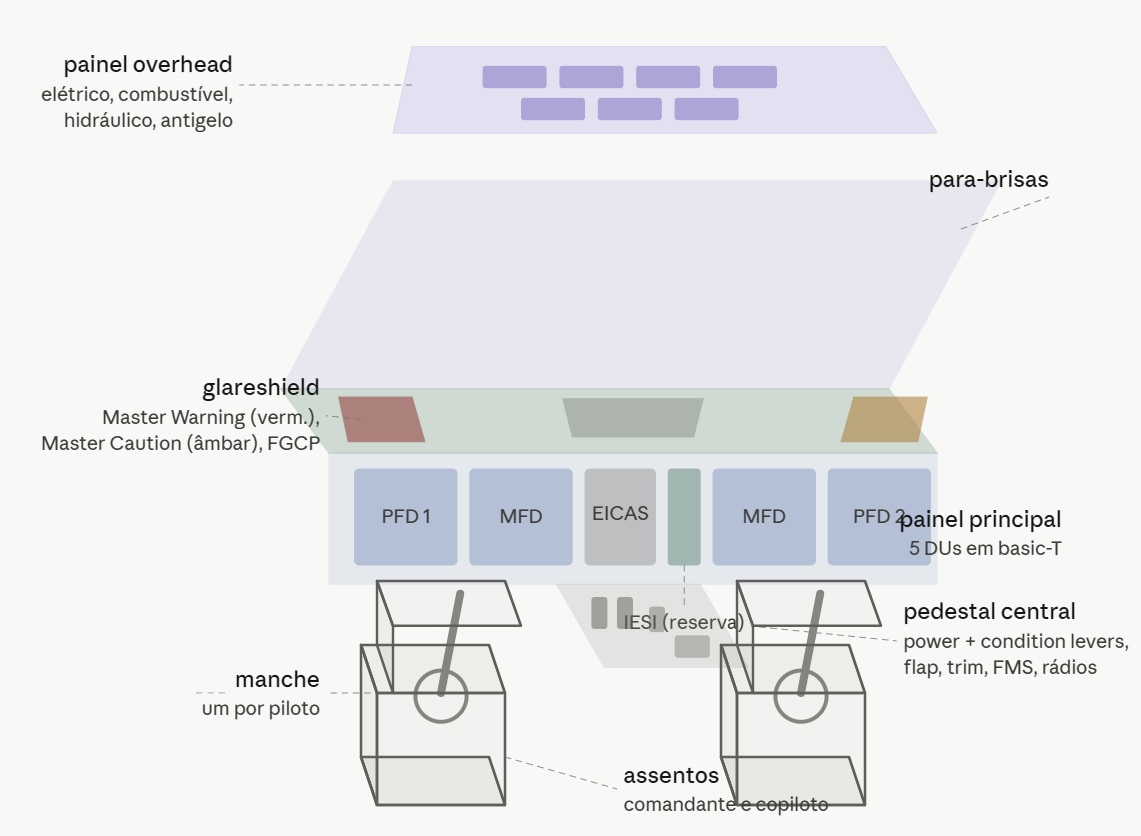
\includegraphics[width=0.75 \linewidth]{esbocopainel.png}
    \caption{Esboço inicial da disposição do painel de instrumentos.}
    \label{fig:painel_frontal}
\end{figure}

A Figura~\ref{fig:integracao_avionicos} apresenta, de forma complementar, a
arquitetura funcional dos principais sistemas aviônicos da aeronave,
evidenciando o fluxo de informações até sua apresentação aos pilotos. As
representações de PFD e MFD nessa arquitetura correspondem às respectivas
funções de apresentação, enquanto sua implementação física no painel é realizada
por dois PFDs e dois MFDs, além do EICAS central.

\begin{figure}[H]
    \centering
        \includegraphics[width=0.9\linewidth]{Figura_3_31.png}
    \caption{Integração dos sistemas de aviônica.}
    \label{fig:integracao_avionicos}
\end{figure}

O PFD constitui a principal interface para apresentação das informações
necessárias à condução da aeronave. Nele são concentrados os parâmetros
fundamentais de voo, permitindo ao piloto acompanhar simultaneamente as
condições de atitude, velocidade, altitude e direção. A concentração dessas
informações mantém a lógica de apresentação associada ao \textit{basic T},
porém em formato digital e integrado.

A Figura~\ref{fig:pfd} apresenta as principais informações que, de acordo com
os requisitos considerados, devem ser disponibilizadas aos pilotos no
\textit{Primary Flight Display}.

\begin{figure}[H]
    \centering
    \includegraphics[width=0.85\linewidth]{Figura_3_32.png}
    \caption{Informações principais do PFD.}
    \label{fig:pfd}
\end{figure}

Os MFDs complementam as informações apresentadas nos PFDs, possibilitando a
visualização de dados de navegação e informações provenientes dos demais
sistemas da aeronave. Essa divisão permite manter os parâmetros fundamentais de
voo permanentemente disponíveis nos PFDs, enquanto informações complementares
podem ser selecionadas e apresentadas nos MFDs conforme a necessidade
operacional.


\subsubsection{Distribuição funcional dos comandos}

Além dos displays principais, o painel de comando é dividido funcionalmente
entre painel frontal, \textit{glareshield}, pedestal central e painel
\textit{overhead}. Essa divisão permite organizar os comandos de acordo com sua
importância operacional, frequência de utilização e necessidade de acesso pela
tripulação.

O \textit{glareshield}, localizado imediatamente acima do painel principal,
acomoda os comandos relacionados ao sistema de orientação de voo e piloto
automático, permitindo sua operação sem grande afastamento da linha de visada
principal. Nessa região também são posicionados os anunciadores de
\textit{Master Warning} e \textit{Master Caution}, permitindo rápida
identificação visual de condições que demandem atenção da tripulação.

O pedestal central, localizado entre os assentos dos pilotos, agrupa os comandos
compartilhados entre os dois postos de pilotagem. Para a configuração
turboélice, são dispostos nessa região os comandos associados aos motores e
hélices, incluindo \textit{power levers} e \textit{condition levers}, além dos
comandos de \textit{flaps}, compensadores e das unidades relacionadas ao
gerenciamento de voo, comunicação e navegação.

Adicionalmente, devido ao fato de o painel ser composto quase integralmente por
displays, com exceção de alguns equipamentos, como a MCDU
(\textit{Multipurpose Control Display Unit}) --- localizada na região inferior
entre os pilotos ---, a unidade \textit{clock}, o sistema ELVE SET
(\textit{Landing Elevation}), entre outros, tais instrumentos são integrados às
regiões funcionais do painel de acordo com sua frequência de utilização e
necessidade de acesso.

O painel \textit{overhead}, por sua vez, aloja principalmente comandos
associados aos sistemas que não necessitam permanecer continuamente no campo
primário de visão dos pilotos, incluindo os sistemas elétrico, hidráulico,
combustível, pressurização, antigelo e partida. Dessa forma, o painel frontal
permanece prioritariamente destinado às informações diretamente relacionadas à
condução e monitoramento do voo.

A organização conjunta dessas regiões busca reduzir a dispersão dos comandos,
facilitar sua identificação e manter as informações e controles de maior
importância operacional nas regiões de melhor visualização e alcance.


\subsubsection{Integração com a ergonomia da cabine}

As dimensões críticas e a posição do painel são estabelecidas a partir dos
critérios antropométricos apresentados na seção anterior. A posição nominal dos
olhos dos pilotos constitui uma referência para a determinação da altura e da
inclinação do painel, bem como para o posicionamento dos displays principais.

A linha normal de visada considerada na análise ergonômica encontra-se
aproximadamente $15^{\circ}$ abaixo da horizontal. Dessa forma, o posicionamento
dos displays principais busca manter as informações de maior relevância
operacional próximas à região natural de visualização dos pilotos, reduzindo a
necessidade de movimentos excessivos da cabeça durante a leitura dos
instrumentos.

Simultaneamente, a borda superior do painel deve preservar o campo de visão
externo através dos para-brisas. A posição do painel, dos olhos dos pilotos e
dos para-brisas é, portanto, considerada de maneira conjunta, de modo a
compatibilizar a leitura dos instrumentos com a visibilidade necessária durante
as operações de táxi, decolagem, aproximação e pouso.

O alcance dos comandos também é relacionado às dimensões antropométricas
adotadas para a cabine. Os comandos de utilização frequente devem permanecer
dentro do alcance funcional dos pilotos na posição normal de operação, enquanto
a distribuição entre painel frontal, \textit{glareshield}, pedestal e
\textit{overhead} deve evitar interferências entre os ocupantes e permitir
acesso adequado aos diferentes sistemas.


\subsubsection{Seleção dos principais equipamentos aviônicos}

Foi realizada uma pesquisa entre modelos de aviônicos comumente
empregados nessa categoria de aeronave, os quais, em sua maioria, possuem
arquitetura remota --- sendo instalados no compartimento de aviônicos da
aeronave. A Tabela~\ref{tab:modelos_avionicos} apresenta alguns dos modelos
encontrados e sugeridos por fabricantes consolidados no mercado, os quais
atendem aos requisitos de certificação TSO e DO-160 necessários para aplicação
aeronáutica.

\begin{table}[H]
    \centering
    \caption{Modelos de aviônicos sugeridos para a aeronave.}
    \label{tab:modelos_avionicos}
    
    \renewcommand{\arraystretch}{1.25}
    \setlength{\tabcolsep}{6pt}
    
    \begin{tabular}{|p{0.24\textwidth}|p{0.18\textwidth}|p{0.19\textwidth}|p{0.30\textwidth}|}
        \hline
        
        \textbf{Equipamento} &
        \textbf{Fabricante} &
        \textbf{Modelo} &
        \textbf{Observação} \\
        \hline
        
        Função VOR/VHF/TCAS &
        Garmin &
        GTN 725 &
        Possui certificação para aplicações em aeronaves ATR 72, podendo ser uma opção para diminuir displays ou ser integrado como \textit{standby}. \\
        \hline
        
        Transponder &
        ACSS &
        NTX-600 &
        Utilizado no ATR e com aplicação comprovada para categoria da aeronave. \\
        \hline
        
        FMS 1 e 2 &
        Thales Group &
        FMS-220 &
        Utilizado no ATR. \\
        \hline
        
        Sistema Radar &
        Honeywell Aerospace &
        RDR-400 &
        Utilizado no EMB-190, que possui aviônicos em comum com o EMB-170. \\
        \hline
        
        Radar Altimeter &
        Honeywell Aerospace &
        KRA-405B com filtro RFF-100 &
        O KRA-405B é o modelo utilizado no EMB-170. O filtro RFF-100 foi uma modificação aprovada para uma aeronave e tem como função reduzir a interferência pelo 5G. \\
        \hline
        
        VOR/ILS &
        Collins &
        VIR-32 &
        Comumente utilizado em muitas aeronaves. \\
        \hline
        
    \end{tabular}
\end{table}


\section{Dimensionamento de Pneus e Freios}
As diretrizes de dimensionamento adotadas baseiam-se nos requisitos de aeronavegabilidade estabelecidos pelo 14 CFR Part 25 da FAA e pelo RBAC 25, aplicáveis a aeronaves de transporte. Para isso, foram adotadas as metodologias de projeto aeronáutico propostas por Daniel P. Raymer e Snorri Gudmundsson, que estão em conformidade com esses requisitos.

\subsection{Distribuição de Cargas no Trem de Pouso}
\label{sec:distribuicao_cargas_tdp}

A distribuição de cargas entre o trem de pouso principal (\textit{Main Landing Gear} - MLG) e o trem de nariz (\textit{Nose Landing Gear} - NLG) é determinada a partir do equilíbrio estático de forças na aeronave. Em configurações triciclo convencionais, o trem de pouso principal suporta aproximadamente 90\% do peso da aeronave, enquanto o de nariz suporta os 10\% restantes.

Para o dimensionamento preliminar, adotou-se essa distribuição de 90\% da carga no MLG e 10\% no NLG, considerando a condição crítica de peso máximo de decolagem (\textit{Weight Takeoff} --- WTO). Conforme recomendado por Raymer e Gudmundsson para aeronaves certificadas sob o FAR Part 25, foi aplicada uma margem adicional de 7\% sobre as cargas estáticas, associada às condições operacionais no solo.  Destaca-se que, apesar de os autores também proporem uma margem de $25 \%$ que pode ser aplicada ao cálculo da cagra máxima, esta é indicada apenas para acrescentar uma folga para possíveis acréscimos de massa na aeronave ao longo de seu dewsenvolvimento. Como este projeto adota o peso máximo de decolagem como pré-requisito, esta margem adicional não se faz necessária. A formulação utilizada para determinação das cargas críticas, então, é dada por:

\begin{equation}
W_{MLG} = \eta_{MLG} \cdot W_{TO} \cdot (1 + \sigma_{FAR}) \cdot (1 + \sigma_{growth})
\end{equation}

\begin{equation}
W_{NLG} = \eta_{NLG} \cdot W_{TO} \cdot (1 + \sigma_{FAR}) \cdot (1 + \sigma_{growth})
\end{equation}

Onde:

\begin{itemize}
    \item $W_{TO} = 50000\ \text{lb}$: peso máximo de decolagem da aeronave;
    
    \item $\eta_{MLG} = 0,90$: fração de carga suportada pelo trem principal;
    
    \item $\eta_{NLG} = 0,10$: fração de carga suportada pelo trem de nariz;
    
    \item $\sigma_{FAR} = 0,07$: margem adicional recomendada para condições operacionais no solo;
    
    \item $\sigma_{growth} = 0,05$: margem de crescimento estrutural.
\end{itemize}

Substituindo os valores adotados nas Equações anteriores, obtêm-se as cargas críticas de projeto para os trens de pouso principal e de nariz:

\begin{equation}
W_{MLG} = 0,90 \cdot 50000 \cdot 1,07 = 48150\ \text{lb} \approx 21840\ \text{kgf}
\end{equation}

\begin{equation}
W_{NLG} = 0,10 \cdot 50000 \cdot 1,07 = 5350\ \text{lb} \approx 2427\ \text{kgf}
\end{equation}

O trem de pouso principal é composto por duas pernas, cada uma equipada com rodas duplas, totalizando quatro pneus ($N_{MLG}=4$). Essa configuração reduz a carga individual por pneu e, consequentemente, a pressão aplicada sobre o pavimento, além de facilitar o alojamento interno do conjunto.

O trem de nariz é constituído por uma única perna com rodas duplas, totalizando dois pneus ($N_{NLG}=2$), configuração adotada para aumentar a estabilidade direcional e a redundância operacional durante as operações em solo.

A partir dessas configurações, determina-se a carga estática atuante em cada pneu individual, considerando as margens de projeto adotadas. Os resultados são apresentados na \autoref{tab:carregamento}.

\begin{table}[H]
    \centering
    \caption{Condições de carregamento do trem de pouso.}
    \vspace{0.2cm}

    \resizebox{\textwidth}{!}{%
    \begin{tabular}{lcccc}
        \toprule
        \textbf{Condição de} & \textbf{Carga Total} & \textbf{Carga Individual} & \textbf{Carga Total} & \textbf{Carga Individual} \\
        \textbf{Carregamento} & \textbf{no MLG (lb/kgf)} & \textbf{por Pneu do MLG (lb/kgf)} & \textbf{no NLG (lb/kgf)} & \textbf{por Pneu do NLG (lb/kgf)} \\
        \midrule
        
        Estática Nominal ($W_{TO}$) 
        & 45000 / 20412 
        & 11250 / 5103 
        & 5000 / 2268 
        & 2500 / 1134 \\
        
        Com Margem FAR Part 25 (+7\%) 
        & 48150 / 21840 
        & 12037,5 / 5460 
        & 5350 / 2427 
        & 2675 / 1213 \\
        
        \bottomrule
    \end{tabular}
    }

    \label{tab:carregamento}
\end{table}


\subsection{Metodologia de Dimensionamento Estatístico}

Antes da seleção definitiva dos pneus a partir de catálogos comerciais, utilizou-se o método estatístico proposto por Raymer \cite{raymer2018} para estimativa preliminar das dimensões dos pneus em aeronaves de transporte civil. O método correlaciona o diâmetro externo ($D_{ext}$) e a largura ($W_{ext}$) do pneu com a carga máxima suportada por roda ($W_w$), em libras.

As correlações utilizadas são:

\begin{equation}
D_{ext} = 1,63 \cdot \left(W_w\right)^{0,315}
\end{equation}

\begin{equation}
W_{ext} = 0,1043 \cdot \left(W_w\right)^{0,480}
\end{equation}

Para o trem de pouso principal, considerando a carga crítica estática com margem regulamentar do FAR Part 25 e sem margem de crescimento estrutural, obtém-se:

\begin{equation}
W_w = \frac{48150}{4} = 12037,5\ \text{lb}
\end{equation}

Substituindo nas Equações anteriores:

\begin{equation}
D_{ext,MLG} = 1,63 \cdot (12037,5)^{0,315}
= 31,54\ \text{in} \approx 801\ \text{mm}
\end{equation}

\begin{equation}
W_{ext,MLG} = 0,1043 \cdot (12037,5)^{0,480}
= 9,48\ \text{in} \approx 240,7\ \text{mm}
\end{equation}

% Considerando também a margem de crescimento estrutural de 25\%:

% \begin{equation}
% W_w = \frac{60.187,5}{4} = 15.046,9\ \text{lb}
% \end{equation}

% \begin{equation}
% D_{ext,MLG} = 1,63 \cdot (15.046,9)^{0,315}
% = 33,81\ \text{in} \approx 859\ \text{mm}
% \end{equation}

% \begin{equation}
% W_{ext,MLG} = 0,1043 \cdot (15.046,9)^{0,480}
% = 10,55\ \text{in} \approx 268\ \text{mm}
% \end{equation}

Para o trem de nariz, considerando a carga crítica estática com margem regulamentar:

\begin{equation}
W_w = \frac{5350}{2} = 2675\ \text{lb}
\end{equation}

\begin{equation}
D_{ext,NLG} = 1,63 \cdot (2675)^{0,315}
= 19,47\ \text{in} \approx 495\ \text{mm}
\end{equation}

\begin{equation}
W_{ext,NLG} = 0,1043 \cdot (2675)^{0,480}
= 4,62\ \text{in} \approx 117\ \text{mm}
\end{equation}


\subsection{Seleção e Especificações de Pneus Comerciais}

Com o objetivo de manter comunalidade com aeronaves da mesma categoria operacional, especialmente o ATR 72, realizou-se a seleção preliminar dos pneus a partir do catálogo da Goodyear Aviation.

Para o trem de pouso principal, optou-se pela utilização de pneus do tipo radial, devido à menor massa estrutural, maior vida útil em ciclos de pouso e melhor desempenho térmico durante frenagens severas.

Para o trem de nariz, selecionou-se um pneu do tipo diagonal (\textit{bias-ply}) equipado com defletor de spray integrado (\textit{chine tire}), solução amplamente empregada em aeronaves turboélice de asa alta para reduzir a projeção de água, detritos e granizo em direção às entradas de ar dos motores durante operações em pista molhada.

\begin{table}[H]
    \centering
    \caption{Especificações dos pneus selecionados para o trem de pouso.}
    \vspace{0.2cm}
    
    \footnotesize
    \setlength{\tabcolsep}{4pt}
    
    \begin{tabular}{p{5.2cm}cc}
        \toprule
        \textbf{Parâmetro Técnico do Fabricante} & \textbf{MLG} & \textbf{NLG} \\
        \midrule
        Tamanho do Pneu (Designação) & H34x10.0R16 & 450x190-5 \\
        Tipo de Construção do Pneu & Radial (Flight Radial) & Diagonal (Flight Leader com Chine) \\
        Part Number (Goodyear) & 346Q48-4 & 459M08-2 \\
        Ply Rating (PR) & 14 & 10 \\
        Carga Homologada (lb/kgf) & 13400 / 6078 & 3822 / 1734 \\
        Pressão Nominal (psi) & 130 & 90 \\
        Diâmetro Máximo Grown (in/mm) & 32,95 / 837 & 17,70 / 450 \\
        Largura Máxima Grown (in/mm) & 9,35 / 237 & 7,50 / 190 \\
        Raio Estático LSD (in/mm) & 14,00 / 356 & 7,05 / 179 \\
        Velocidade Limite (mph / kt) & 190 / 165 & 190 / 165 \\
        Roda / Flange (in) & 16,0 / 7,00 & 5,0 \\
        \bottomrule
    \end{tabular}
    
    \label{tab:pneus_selecionados}
\end{table}


Ainda segundo Raymer \cite{raymer2018}, a pressão operacional dos pneus pode ser ajustada para valores calculados proporcionalmente à pressão nominal em situações de operação abaixo da carga nominal, de modo que:

\begin{equation}
    P_{op}= P_{nom}\frac{W_{op}}{W_{nom}}
\end{equation}

Assim, considerando-se uma pressão nominal de 130 psi, carga operacional de 11250 lb e carga nominal de 13400 lb para o MLG, enquanto esses respectivos valores são de 90 psi, 2500 lb e 3822 lb para o NLG, calcula-se pressões operacionais de 109,15 psi e 58,9 psi para os pneus do trem de pouso principal e de nariz, respectivamente. 

\subsubsection{Análise Comparativa e Validação Física}
Ao comparar os pneus selecionados com as estimativas preliminares obtidas pelo método de Raymer, observa-se boa concordância entre os valores calculados e os dados de catálogo. O pneu principal selecionado apresenta diâmetro externo de 32,95 in, correspondendo a um desvio de aproximadamente +4,5\% em relação ao valor estimado de 31,54 in. A largura nominal de 9,35 in difere em aproximadamente -1,0\% da estimativa de 9,45 in.

A capacidade de carga homologada do pneu H34x10.0R16, igual a 13400 lb, atende à carga regulamentar por roda de 12037,5 lb com margem de aproximadamente 11,3\%.

\subsection{Análise Física do Flanco do Pneu e Operabilidade}

A escolha da geometria do flanco (altura lateral da borracha) constitui um compromisso crítico de projeto entre eficiência aerodinâmica e capacidade de amortecimento no solo. A altura do flanco ($H$) é obtida pela equação:

\begin{equation}
H = \frac{D_{\max} - D_{rim}}{2}
\end{equation}

Onde $D_{\max}$ é o diâmetro externo Grown e $D_{rim}$ é o diâmetro nominal da roda (aro).

\subsubsection*{Pneu Principal (H34x10.0R16)}

\begin{equation}
H_{MLG} = \frac{(32,95 - 16,0)}{2} = 8,475 \ \text{in} \ (\approx 215,3 \ \text{mm})
\end{equation}

A relação de aspecto do flanco em relação à largura do pneu é:

\begin{equation}
\zeta_{MLG} = \frac{H_{MLG}}{w} = \frac{8,475}{9,35} \approx 0,906 \ (90,6\%)
\end{equation}

\subsubsection*{Pneu de Nariz (450x190-5)}

\begin{equation}
H_{NLG} = \frac{(17,70 - 5,0)}{2} = 6,35 \ \text{in} \ (\approx 161,3 \ \text{mm})
\end{equation}

A relação correspondente é:

\begin{equation}
\zeta_{NLG} = \frac{H_{NLG}}{w} = \frac{6,35}{7,50} \approx 0,847 \ (84,7\%)
\end{equation}

A manutenção de uma alta relação de aspecto do flanco ($\zeta > 80\%$) reflete a orientação de projeto estabelecida nesse trabalho para operação em pistas semi-preparadas ou com revestimentos asfálticos deteriorados de aeródromos regionais. O pneu de perfil alto funciona como um sistema secundário de absorção de choque pneumático. Sob impactos verticais causados por detritos ou buracos na pista, a grande deflexão do flanco distribui as forças, reduzindo o estresse dinâmico de pico transmitido à estrutura de fixação do trem de pouso na fuselagem e mitigando os efeitos de fadiga.

Em contrapartida, pneus de perfil baixo e flanco curto, comuns em jatos comerciais rápidos, são projetados estritamente para altas velocidades e pistas perfeitamente lisas, pois minimizam o arrasto e os movimentos de inclinação lateral nas curvas (\textit{rolling stiffness}), porém transmitem impactos de forma severa para a estrutura da aeronave.

A pressão de inflação nominal do pneu do trem principal de $115 \ \text{psi}$ e do trem de nariz de $90 \ \text{psi}$ classifica a aeronave na faixa de pressão intermediária, adequada para operações em pistas de asfalto ou concreto de média resistência, mantendo excelente coeficiente de atrito.


\subsection{Dimensionamento e Análise dos Freios}

\subsubsection{Determinação da Velocidade de Decisão de Decolagem ($V_1$)}

O dimensionamento térmico e mecânico do sistema de freios deve ser conduzido com base
no cenário crítico de \textbf{Decolagem Rejeitada} ($R_{TO}$),
conforme prescrito pelo parágrafo § 25.735(f)(2) do RBAC~25. Nessa condição, a aeronave
se encontra no seu \textbf{Peso Máximo de Decolagem} (MTOW) e a frenagem de emergência
é iniciada na velocidade de decisão $V_1$, que é inerentemente superior à velocidade de
toque de pouso convencional. Por esse motivo, o RTO representa o caso de carregamento
crítico que dita a capacidade térmica mínima do conjunto freio--roda.

A velocidade de decisão de decolagem $V_1$ é estimada de forma conservadora em:

\begin{equation}
    V_1 = 105 \ \text{kt}
\end{equation}

Este valor é compatível com o envelope operacional de decolagem da aeronave de
referência ATR~72-600 (cujo $V_2 \approx 116\ \text{kt}$) e representa uma estimativa
conservadora para projeto preliminar. Convertendo para o sistema imperial:

\begin{equation}
    V_1 = 105 \times 1{,}68781 \approx 177{,}22 \ \text{ft/s}
\end{equation}


\subsubsection{Cálculo da Energia Cinética de Frenagem — Caso $R_{TO}$}

A capacidade térmica mínima do sistema de freios é determinada a partir da energia
cinética total que os freios devem absorver integralmente durante uma parada de
emergência em RTO. Adota-se a condição mais conservadora, sem contribuição de
empuxo reverso nem de arrasto aerodinâmico.

A energia cinética total da aeronave no instante de início da frenagem é dada por:

\begin{equation}
    KE_{total} =
    \frac{1}{2}
    \left(
        \frac{W_{TO}}{g}
    \right)
    V_1^{\,2}
\end{equation}

Onde:

\begin{equation}
    W_{TO} = 50\,000 \ \text{lb}
\end{equation}

\begin{equation}
    g = 32{,}174 \ \text{ft/s}^2
\end{equation}

\begin{equation}
    V_1 = 177{,}22 \ \text{ft/s}
\end{equation}

Substituindo os valores:

\begin{equation}
    KE_{total} =
    \frac{1}{2}
    \left(
        \frac{50\,000}{32{,}174}
    \right)
    (177{,}22)^2
\end{equation}

\begin{equation}
    KE_{total}
    \approx
    24\,379\,000 \ \text{ft-lbf}
\end{equation}

Considerando quatro rodas freadas no trem de pouso principal:

\begin{equation}
    N_{freios} = 4
\end{equation}

A energia cinética absorvida por cada conjunto de freio é:

\begin{equation}
    KE_{roda} =
    \frac{KE_{total}}{N_{freios}}
    =
    \frac{24\,379\,000}{4}
\end{equation}

\begin{equation}
    KE_{roda}
    \approx
    6\,094\,750 \ \text{ft-lbf}
\end{equation}

Convertendo para Joules ($1\ \text{ft-lbf} = 1{,}35582\ \text{J}$):

\begin{equation}
    KE_{roda}
    = 6\,094\,750 \times 1{,}35582
    \approx 8\,263\,000 \ \text{J}
\end{equation}

\begin{equation}
    \boxed{KE_{roda} \approx 8{,}26 \ \text{MJ}}
\end{equation}

Adota-se portanto $KE_{projeto} = 8{,}26\ \text{MJ}$ como capacidade térmica mínima
por conjunto freio--roda para o dimensionamento do sistema de freios, em conformidade
com o caso crítico regulatório de Decolagem Rejeitada exigido pelo § 25.735(f)(2)
do RBAC~25.

\subsection{Seleção da Tecnologia de Freios}

A dissipação de aproximadamente $8,26, \ \text{MJ}$ por roda impõe elevada solicitação térmica ao sistema de frenagem, exigindo materiais com alta resistência térmica e estabilidade estrutural. Para a aeronave, adotou-se o uso de freios multidisco de carbono em substituição aos conjuntos convencionais de aço.

As principais características e impactos dessa escolha são apresentados na \autoref{tab:comparacao_freios}.

\begin{table}[H]
    \centering
    \caption{Comparação entre tecnologias de freios aeronáuticos.}
    \vspace{0.2cm}

    \renewcommand{\arraystretch}{1.6}
    \setlength{\tabcolsep}{6pt}

    \begin{tabular}{|p{3.5cm}|p{3.2cm}|p{3.5cm}|p{5.2cm}|}
        \hline
        \textbf{Propriedade / Característica} &
        \textbf{Freios de Aço} &
        \textbf{Freios de Carbono} &
        \textbf{Impacto Técnico no Projeto} \\
        \hline

        Peso do Conjunto de Freios
        & Elevado (referência)
        & Redução de 35\% a 42\% em massa
        & Redução do OEW e aumento da capacidade de carga paga ou combustível \\
        \hline

        Condutividade Térmica
        & Moderada
        & Elevada
        & Dissipação térmica mais eficiente e menor risco de superaquecimento \\
        \hline

        Resistência Térmica e Vida Útil
        & Perda de eficiência acima de $500^\circ$C; vida útil entre 800 e 1200 ciclos
        & Operação estável até $1200^\circ$C; vida útil entre 1500 e 3000 ciclos
        & Maior confiabilidade operacional e redução de manutenção \\
        \hline

        Custo de Aquisição Inicial
        & Baixo
        & Elevado
        & Maior custo inicial compensado pela durabilidade e menor custo operacional \\
        \hline
    \end{tabular}

    \label{tab:comparacao_freios}
\end{table}


\subsection{Sistema de Atuação Hidráulica e Segurança}

O acionamento do trem de pouso e do sistema de freios é realizado por um sistema hidráulico operando a $3.000 \ \text{psi}$, alimentado por bombas acopladas à caixa de acessórios dos motores PW127M. A arquitetura hidráulica é dividida em circuitos redundantes para atendimento aos requisitos de segurança do RBAC 25.

\begin{itemize}
    \item \textbf{Circuito Hidráulico Primário de Retração e Frenagem:} responsável pelo acionamento dos atuadores de recolhimento do trem de pouso e pelo fornecimento de pressão hidráulica às pinças de freio do trem principal, com sistema anti-skid.

    \item \textbf{Circuito Hidráulico Secundário:} atua automaticamente em caso de falha do circuito primário, mantendo capacidade residual de frenagem e esterçamento do trem de nariz.

    \item \textbf{Extensão de Emergência por Gravidade:} em caso de perda total de pressão hidráulica, o sistema libera os mecanismos de travamento superior (\textit{uplocks}), permitindo a extensão do trem de pouso por gravidade e arrasto aerodinâmico, com travamento mecânico na posição abaixada.
\end{itemize}

\subsection{Geometria de Alojamento do Trem de Pouso em Asa Alta}

Na configuração de asa alta, o recolhimento do trem principal diretamente para o interior da asa exigiria o comprimento do trem de pouso excessivamente grande, aumentando peso e momentos fletores quando em contato com o solo. Para evitar essa limitação, o trem principal é fixado às estruturas inferiores da fuselagem e recolhido lateralmente para carenagens externas do tipo \textit{sponson}, solução utilizada em aeronaves como ATR 72 e CASA C-295.

Esse arranjo apresenta as seguintes vantagens:

\begin{itemize}
    \item preservação da caixa de torção da asa (\textit{wing box}) para cargas aerodinâmicas e armazenamento de combustível;

    \item redução do comprimento das pernas do trem de pouso e, consequentemente, da massa estrutural do sistema;

    \item simplificação do mecanismo de retração hidráulica por rotação lateral com travamento por tesoura.
\end{itemize}

O trem de nariz é recolhido para a região frontal da fuselagem, abaixo do cockpit. O recolhimento para frente favorece o travamento aerodinâmico em caso de falha hidráulica.

\subsection{Posicionamento do trem de pouso}
\label{sec:posicionamento_tdp}

\subsubsection{Comprimentos}

Pelo FAR Part 25, há a exigência de que a hélice esteja a pelo menos $7"$ do solo, ou 178 mm. Com isso, a partir da clearance lateral exigida, conforme Trahmer, na figura \ref{fig:lateral clearence} e pela geometria, foi possível estimar uma altura de 0,70 m para os trens de pouso, considerando que a aeronave ficará nivelada em solo.

\begin{figure}[H]
    \centering
    \begin{minipage}{0.8\textwidth} % Ajuste o 0.8 para aumentar ou diminuir o tamanho
        \centering
        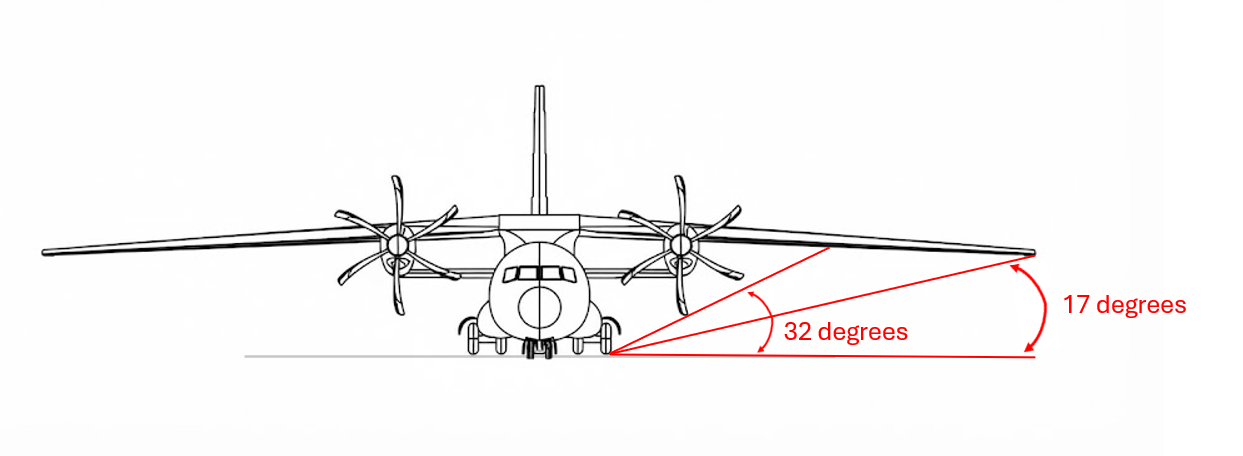
\includegraphics[width=\linewidth]{images/Altura aeronave.png}
        \caption{Requeirmento de clearance lateral}
        \label{fig:lateral clearence}
    \end{minipage}
\end{figure}

\subsubsection{Posicionamento}

Os componentes do trem de pouso têm que ser posicionados de forma a evitar que a aeronave tombe ao realizar manobras em solo. Isso é feito de forma a posicionar cada perna em relação ao CG, de 10,82 m a partir do nariz e de 0,59 m a partir do ponto mais baixo da fuselagem.

Naturalmente, o NLG, por ser constituido de apenas uma perna, é posicionado na linha de simetria da aeronave.
A partir do requerimento de ângulo de turnover mostrado na figura \ref{fig:trem lateral} e o CG vertical de 0,59 m, é possível apontar que a bitola fica em torno de 4,1 m.

\begin{figure}[H]
    \centering
    \begin{minipage}{0.8\textwidth} % Ajuste o 0.8 para aumentar ou diminuir o tamanho
        \centering
        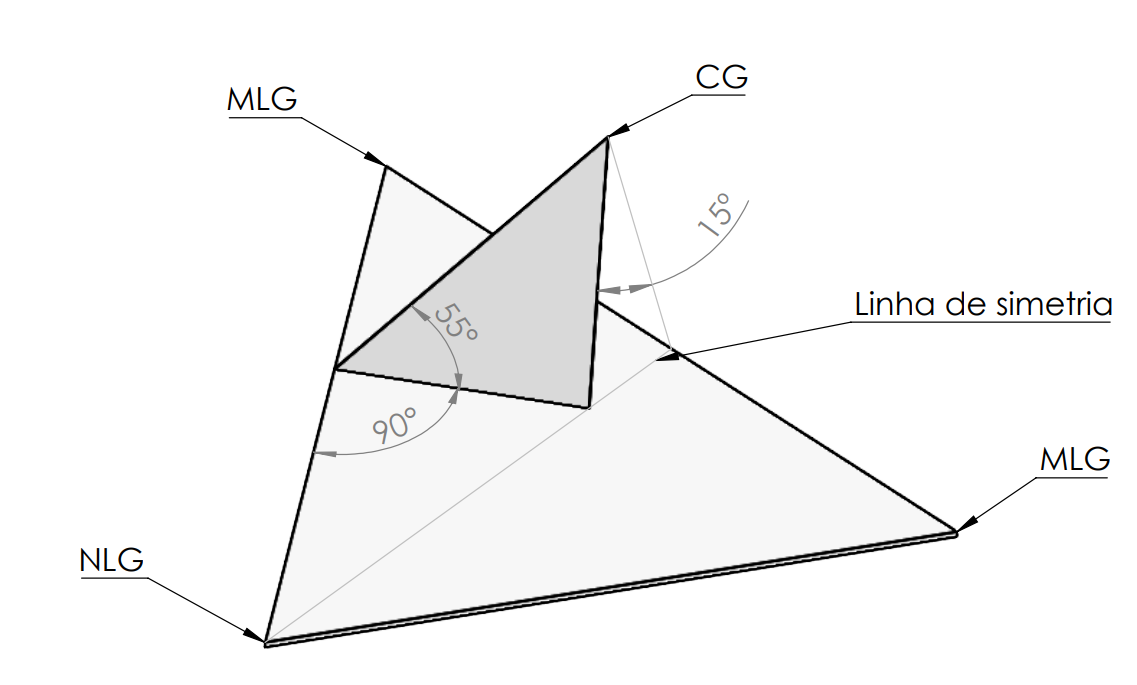
\includegraphics[width=\linewidth]{images/Posição lateral do trem de pouso.png}
        \caption{Posição lateral do trem de pouso.}
        \label{fig:trem lateral}
    \end{minipage}
\end{figure}

Já em relação ao posicionamento longitudinal, o trem de pouso de nariz foi arbitrariamente posicionado a 1,87 m do nariz. Esse valor vem da análise comparativa e corrobora com a estrutura interna da aeronave, ajustado posteriormente com base no avanço do projeto.

Já o trem de pouso principal deve estar posicionado de forma que a linha entre o CG e o MLG forme um ângulo de no mínimo 15° com a vertical. Com base na geometria, foi obtido que a distância entre o NLG e o MLG é de 9,0 m.

\begin{figure}[H]
    \centering
    \begin{minipage}{0.8\textwidth} % Ajuste o 0.8 para aumentar ou diminuir o tamanho
        \centering
        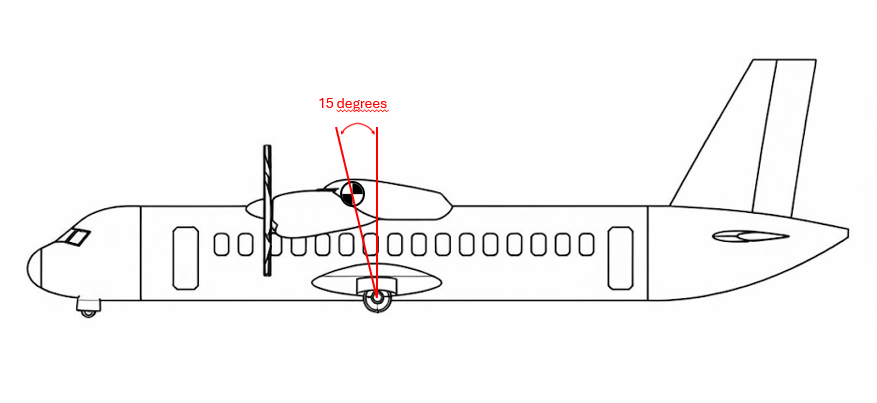
\includegraphics[width=\linewidth]{images/posicionamento longitudinal do trem de pouso.png}
        \caption{Posionamento longitudinal do trem de pouso.}
        \label{fig:longitudinal}
    \end{minipage}
\end{figure}


\subsubsection{Configuração final}

A configuração final foi confirme a imagem \ref{fig:configuração final do trem de pouso}.

\begin{figure}[H]
    \centering
    \begin{minipage}{0.8\textwidth} % Ajuste o 0.8 para aumentar ou diminuir o tamanho
        \centering
        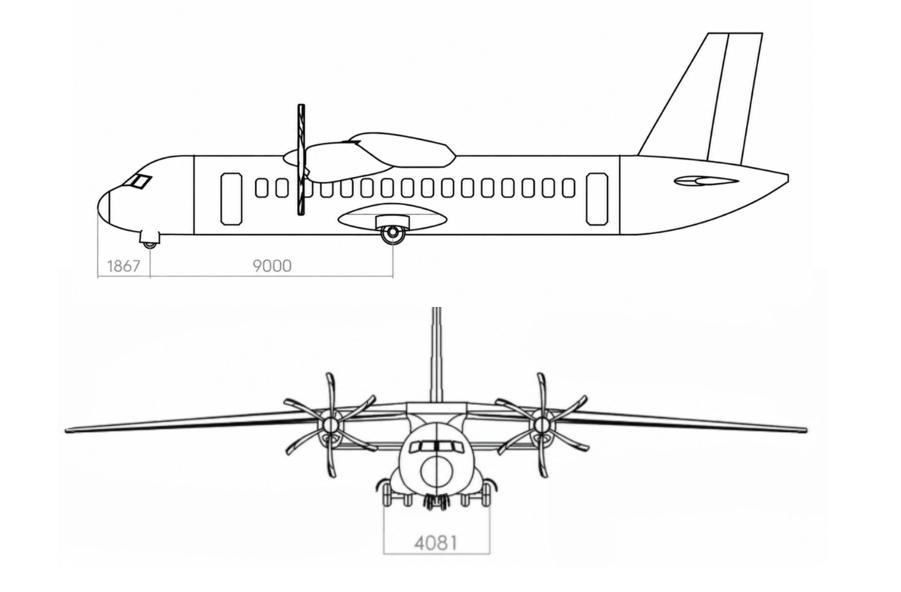
\includegraphics[width=\linewidth]{images/final trem de pouso.png}
        \caption{Configuração final do trem de pouso.}
        \label{fig:configuração final do trem de pouso}
    \end{minipage}
\end{figure}

\section{Dimensionamento de Sistemas}

\subsection{Sistema Hidráulico}

De acordo com o regulamento 14 CFR Part 25, Seção 25.1435, os componentes conectados ao sistema hidráulico principal devem ser projetados para suportar pressões de teste e de ruptura estabelecidas em função da Design Operating Pressure (DOP). Por meio de uma análise comparativa com aeronaves comerciais de porte semelhante, decidiu-se a utilização de uma DOP de 3000 psi, que representa uma prática comum da indústria para essa categoria de aeronaves. Dessa forma, esse valor foi adotado como pressão de operação de projeto para o dimensionamento preliminar do sistema hidráulico.\\
Além disso, a Design Operating Pressure (DOP) influencia diretamente o dimensionamento dos atuadores hidráulicos, uma vez que, para uma mesma força requerida, o aumento da pressão de operação permite a utilização de cilindros com menor área efetiva. Entretanto, pressões mais elevadas demandam componentes mais robustos, sofisticados e de maior custo, característica comum em aeronaves de transporte de passageiros de maior porte.\\
Para a elaboração do diagrama simplificado do sistema hidráulico, além do atendimento aos requisitos normativos, foi utilizado como referência o manual da aeronave ATR 72-600, por se tratar do modelo com características operacionais e de porte mais semelhantes à aeronave desenvolvida neste trabalho.\\
 A tabela abaixo foi estruturada com base na tabela original do regulamento, a qual encontra-se disponível na página 96, seção 25.1435, item a.
\begin{table}[H]
\centering
\caption{Fatores de pressão de ensaio e pressão última para componentes do sistema hidráulico.}
\label{tab:pressao_hidraulica}

\begin{tabular}{|p{8cm}|c|c|}
\hline
\textbf{Elemento} & \textbf{Ensaio (xDOP)} & \textbf{Última (xDOP)} \\
\hline
Tubulações e conexões & 4.500 psi & 9.000 psi\\
\hline
Vasos de pressão contendo gás (alta pressão, ex.: acumuladores) & 9.000 psi& 12.000 psi\\
\hline
Vasos de pressão contendo gás (baixa pressão, ex.: reservatórios) & 4.500 psi & 9.000 psi \\
\hline
Mangueiras & 6.000 psi & 12.000 psi \\
\hline
Demais componentes & 4.500 psi& 6.000 psi \\
\hline
\end{tabular}
\end{table}
 Adicionalmente, o requisito exige que os integrantes do sistema sejam capazes de suportar a pressão operacional de projeto juntamente com as cargas estruturais máximas previstas sem deformação que prejudique sua função, isto inclui suportar as cargas aerodinâmicas, as cargas devido a pressão interna, a vibrações, entre outras. Ademais, a tripulação deve ser informada imediatamente em caso de algum tipo de falha e possui meios para monitorar e ser alertada em caso de algum problema do sistema.\\
 Em resumo, o regulamento exige que:
 \begin{itemize}
     \item Cada componente suporte as pressões indicadas na Tabela \ref{tab:pressao_hidraulica};
     \item O sistema suporte cargas estruturais e vibrações;
     \item Não ocorram rupturas mesmo em condições extremas;
     \item Deve haver proteção contra ciclos de fadiga;
     \item Monitoramento pela tripulação;
     \item Vazamentos perigosos sejam minimizados;
     \item O sistema seja validado por testes de desempenho, fadiga e operação em voo.
 \end{itemize}
\vspace{0.5 cm}

 Para cumprir as exigências precisamos assegurar que alguns critérios sejam satisfeitos:
 \begin{itemize}
     \item As informações do sistema hidráulico precisam ser exibidas no cockpit;
     \item Deve haver alguma redundância para minimizar as chances de falha;
     \item Deve haver alertas sonoros para falhas e alerta emitidos para indicar que o sistema está apto, exemplo: PTU do A320.
     \item Em caso de falha nem todo sistema poderá ser comprometido;
     \item As bombas hidráulicas precisam ter acionamento via fonte AC e, quando disponível, fonte DC, para o caso em que as baterias estiverem suprindo a demanda.
 \end{itemize}

 Dessa forma, além dos critérios acima estabelecidos e levando em consideração o estudo do sistema hidráulico do ATR 72-600 um diagrama simplificado do sistema foi elaborado conforme abaixo:

A imagem acima apresenta uma versão simplificada da arquitetura do sistema hidráulico proposto, destacando seus principais componentes. De maneira semelhante à aeronave de referência, o sistema é composto por dois circuitos hidráulicos independentes, responsáveis pelo fornecimento do fluxo hidráulico aos consumidores da aeronave.\\
Ambos os circuitos são interligados por uma válvula de controle acionada por meio de um \textit{\textbf{push button}}, permitindo a transferência de fluido entre os sistemas em caso de falha de um dos retornos. Dessa forma, garante-se a continuidade do fornecimento hidráulico aos equipamentos essenciais da aeronave.\\
Adicionalmente, cada sistema possui seu próprio acumulador hidráulico e um conjunto independente de alimentação elétrica para as bombas hidráulicas. O sistema azul é alimentado pelo barramento elétrico BUS 1, enquanto o sistema verde é alimentado pelo BUS 2. Essa segregação aumenta a confiabilidade do projeto, uma vez que uma eventual falha elétrica em um dos barramentos não compromete completamente a capacidade de geração e distribuição de potência hidráulica da aeronave.\\
O reservatório hidráulico possui níveis de monitoramento destinados à detecção precoce de falhas e à garantia da operação segura do sistema. Um alerta de baixa quantidade de fluido deve ser acionado quando o nível atingir o valor indicado pela terceira linha preta pontilhada. Esse alerta tem caráter preventivo e visa informar a tripulação sobre a necessidade de inspeção ou manutenção do sistema.\\
Além disso, um alerta de emergência deve ser apresentado no cockpit caso o nível de fluido atinja a linha vermelha, correspondente ao limite mínimo admissível definido em projeto. Nessa condição, a quantidade de fluido disponível pode não ser suficiente para atender às demandas hidráulicas críticas da aeronave, comprometendo a confiabilidade e a disponibilidade do sistema. \\
Para calcular a  mínima de capacidade de fluído que deve estar disponível em tanque, um procedimento simplificado foi adotado, considerando a equação de momento em torno das articulações das superfícies de comando (Equação \ref{eq:moment-articu}), margem de segurança e sistema de frenagem.
\begin{equation}
    H = \frac{1}{2} \cdot \rho \cdot V \cdot S_c \cdot \bar{\bar{c_c}} \cdot C_H
    \label{eq:moment-articu}
\end{equation}
Em que:
\begin{itemize}
    \item V é a velocidade crítica das condições analisadas, sendo essas a VA e VD ;
    \item $S_c$ é a área da superfície;
    \item $\bar{\bar{c_c}}$ é  acorda média aerodinâmica da superfície analisada;
    \item $C_H$ é o coeficiente de momento em torno da articulação.
\end{itemize}

O coeficiente de momento por sua vez, pode ser descrito pela linearização abaixo, disponível nas notas de aulas de Estabilidade e Controle Ricardo U. Pinto (2012):
\begin{equation}
    C_H= b_0 + b_1 \cdot \alpha +b_2 \cdot \eta + b_3 \cdot \delta
\end{equation}
Considerou-se que as superfícies possuem perfis simétricos e com isso $b_0$ torna-se nulo, adicionalmente, descartou-se o uso de compensador e dessa forma a parcela de $b_3$ torna-se nula, asssim:
\begin{equation*}
    C_H = b_1 \cdot \alpha + b_2 \cdot \eta
\end{equation*}
As constantes $b_1$ e $b_2$ foram estimadas com base na aproximação proposta por ROSKAM, Jan. Airplane Design, Part VI em que:

\begin{equation}
\begin{aligned}
    b_1 &= C_{h_\alpha} \cdot D \\[6pt]
    b_2 &= C_{h_\delta} \cdot D
\end{aligned}
\end{equation}
Em que $C_{h_\alpha}$ e $C_{h_\delta}$ são estimados conforme as Figuras 10.63b e 10.69b do capítulo 10 de ROSKAM, Jan. Airplane Design, Part VI, respectivamente. Adicionalmente, o fator de correção 3D (D) é estimado por:
\begin{equation}
    D = \frac{C_{L_\alpha}}{C_{l_\alpha}}
\end{equation}

No qual o valor de $C_{L_\alpha}$ foi considerado como sendo o do avião sem flap e que foi obtido já com as correções para análise tridimensional da aeronave, $C_{l_\alpha}$ é aproximado por $2 \cdot \pi $ [$rad^{-1}$].\\
Assim obteve se um $C_H$ para cada superfície de controle principal e com isso o momento de cada superfície de controle principal (leme, aileron e profundor). Posteriormente, utilizou-se da pressão padrão de operação definida (DOP) e da seguinte formulação para calcular o volume de fluído requerido por essas superfícies.

\begin{equation}
    Volume = \frac{\frac{H}{braço}}{DOP } \cdot curso \cdot 1000
\end{equation}

De modo que o braço e curso foram baseados em método comparativo e pesquisa por valores padronizados na aviação, estimados em medições a partir do datum em catálogos de peças. \\
Assim, obtemos o volume para o acionamento das superfícies. Com relação ao freio e trem de pouso foi adotado o seguinte procedimento:

\begin{itemize}
    \item Para o trem de pouso, considerou-se para o cálculo que sua massa correspondia a 4,5\% do MTOW;
    \item  Um fator de arrasto e um curso de atuação foram estimados de modo que os resultados fossem compatíveis com os da aeronaves similares;
    \item Assim estimou-se a área e por fim o volume com base na DOP;
    \item Para os freios, considerou-se as quatro rodas e os quatro pistões por roda;
    \item Considerou-se um curso de 10 cm para os freios e uma área foi adotada para o pistão com base em um diâmetro de 85 mm, estimativa em escala;
    \item Obtendo assim o volume de fluído requerido pelos freios.
\end{itemize}

Dessa forma, foi realizada uma estimativa do consumo de fluido hidráulico considerando os atuadores das superfícies de comando sem a utilização de horn. Para a análise, foram consideradas apenas as condições correspondentes às velocidades de manobra ($V_A$) e de mergulho ($V_D)$). A partir dessas condições, foram obtidos os seguintes valores de capacidade  requerida para o reservatório hidráulico:

\begin{table}[H]
\centering
\caption{Dimensionamento do tanque hidráulico.}
\label{tab:dimensionamento_tanque}
\begin{tabular}{|c|c|c|}
\hline
\textbf{Velocidade} & \textbf{Demanda Simultânea Crítica} & \textbf{Volume com fator de tanque 1,2} \\
\hline
$V_A$ & 5.29 L & 6.96L \\
\hline
$V_D$ & 7,54 L & 9,63L \\
\hline
\end{tabular}
\end{table}


Portanto, considerando as hipóteses conservadoras adotadas no dimensionamento, obteve-se um reservatório hidráulico com capacidade máxima de 9,63 L. Adicionalmente, foi definido que o sistema deverá emitir um alerta de baixa quantidade de fluido quando o volume armazenado atingir 5,31 L.

Vale ressaltar que os valores obtidos mostram-se coerentes com aqueles encontrados em aeronaves da mesma categoria. Tendo em vista a referência adotada, o ATR 72-600 possui um reservatório hidráulico com capacidade máxima de aproximadamente 9,6 L, evidenciando que o dimensionamento realizado encontra-se dentro da faixa esperada para a aplicação considerada.



\begin{figure}[H]
    \centering
    \begin{minipage}{0.45\textwidth}
        \centering
        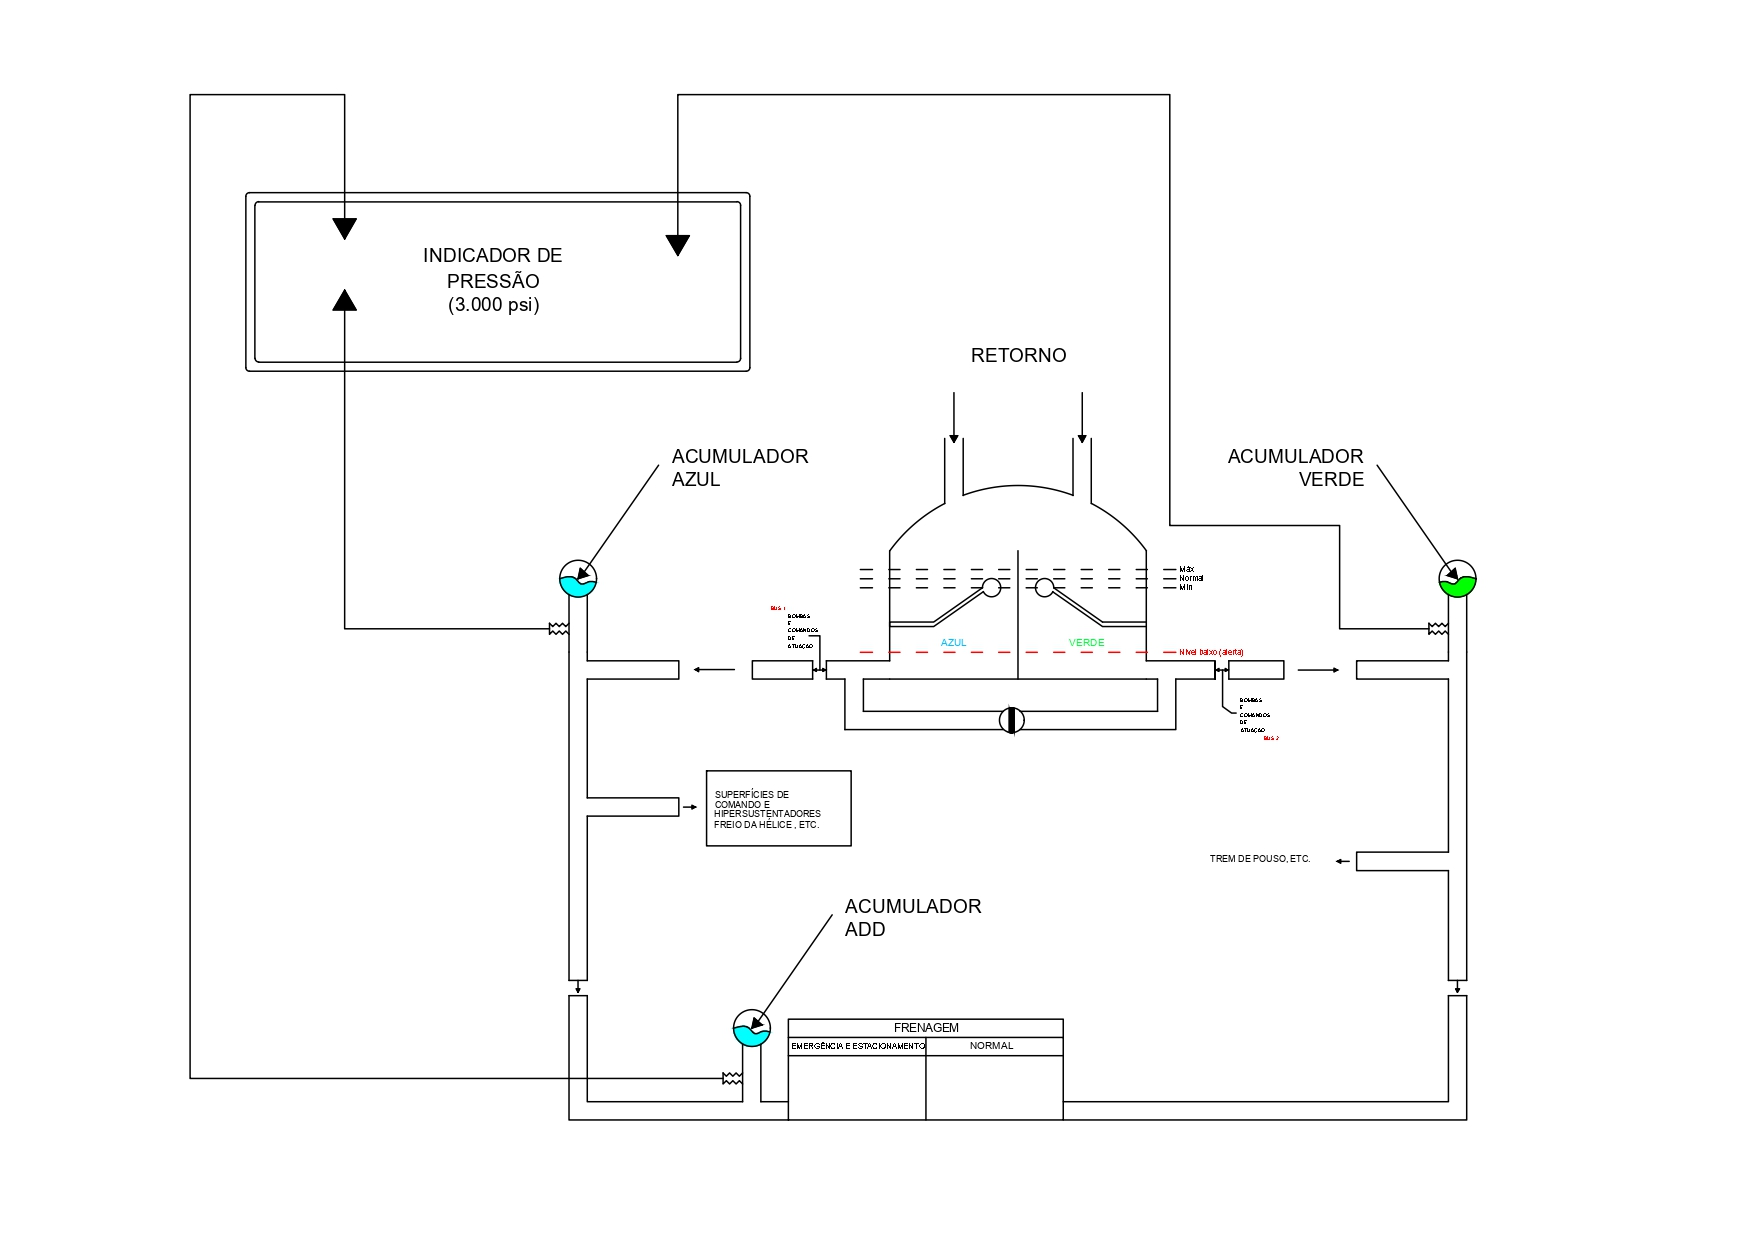
\includegraphics[width=\linewidth]{images/SistemaHidraulico.jpg}
        \caption{Diagrama simplificado do sistema hidráulico.}
        \label{sys_hidraulico}
    \end{minipage}
    \hfill
    \begin{minipage}{0.45\textwidth}
        \centering        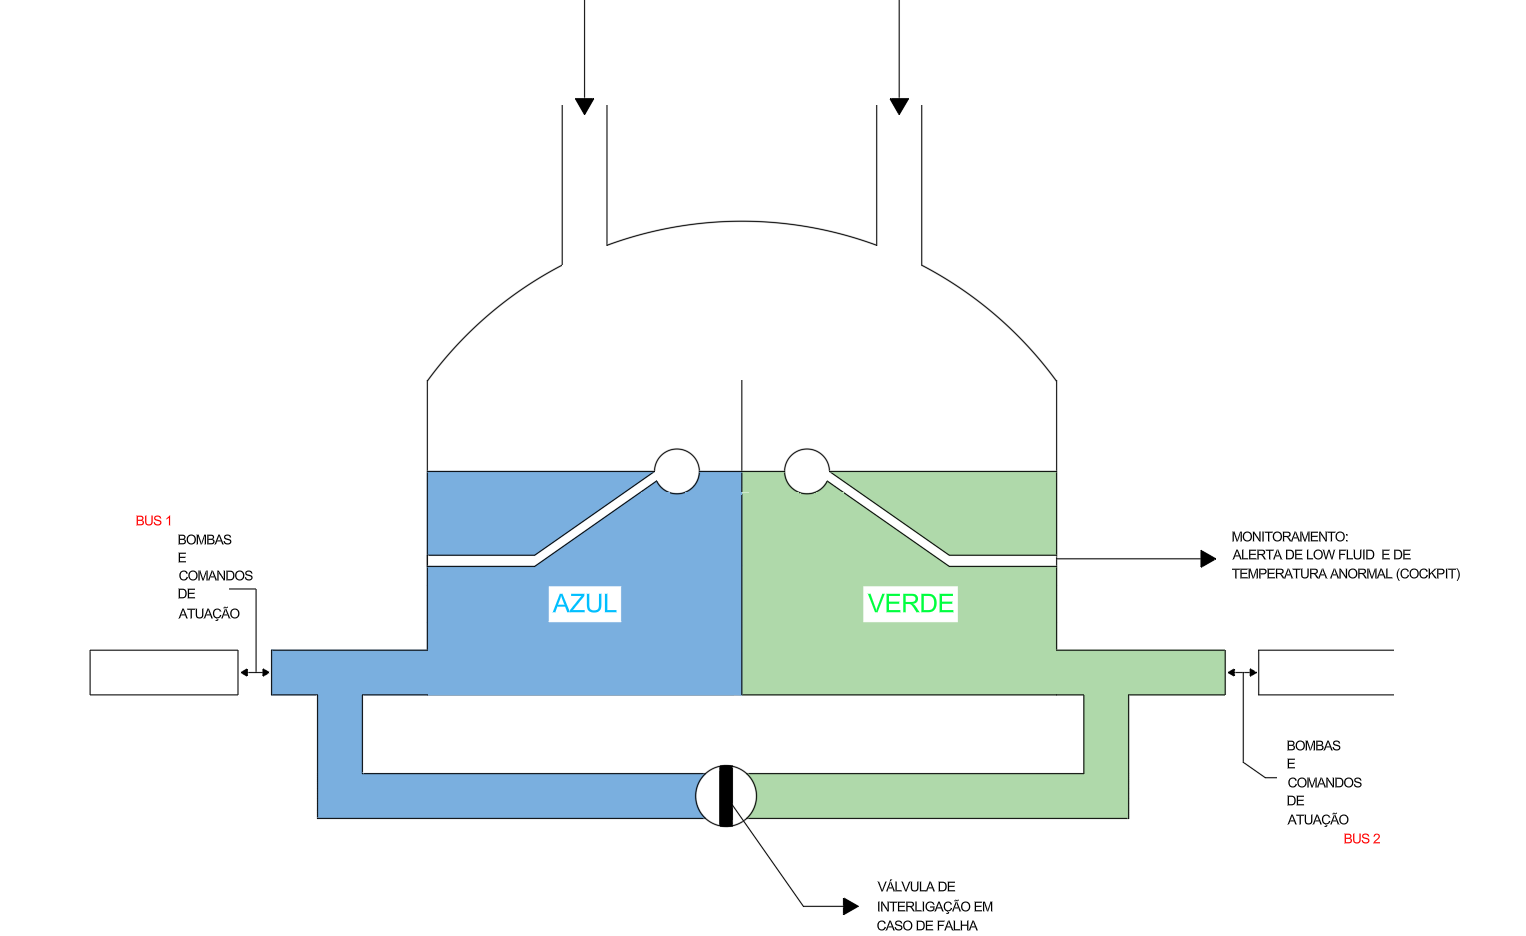
\includegraphics[width=\linewidth]{images/RESERVATÓRIO.png}
        \caption{Reservatório do fluido hidráulico}
        \label{Reservatorio_hidr}
    \end{minipage}
\end{figure}

\subsection{Environmental Control System}

O  ECS (\textit{Environmental Control System}) é responsável por garantir condições ambientais adequadas aos ocupantes da aeronave, proporcionando conforto e segurança. Suas principais funções incluem o fornecimento e a distribuição de ar para a cabine, o controle da temperatura, a remoção de contaminantes e a manutenção da pressão interna em níveis adequados. O dimensionamento preliminar foca apenas no sistema de pressurização da cabine e no sistema de ar-condicionado.

Conforme o requisito §25.841, aeronaves certificadas para operação até $25000 \ ft$, como este projeto, devem ter uma altitude máxima de cabine de $8000 \ ft$. Usando a atmosfera ISA, pode-se calcular o diferencial de pressão máximo no teto operacional.

\begin{equation}
    \Delta P=P_{cab}-P_{FL250}=10,92-5,45=5,47 \ psi
\end{equation} 

Deve haver uma válvula de alívio de pressão positiva para evitar a hiperpressurização. Considerando o valor típico de $\Delta P+0,5$, a válvula de ser dimensionada para $6,0 \ psi$. Para a válvula de alívio de pressão negativa (indispensável em situação de emergência de descida rápida), recomenda-se o dimensionamento para $-0,5 \ psi$. Posteriormente, o diferencial máximo da válvula de alívio será utilizado no cálculo de tensões circunferenciais e longitudinais na fuselagem. 

O balanço de massa deve ser feito para o dimensionamento preliminar dos PACK's - \textit{Pressurization Air Conditioning Kit}. Tem-se:
\begin{equation}
    \dot{m}_{supply}=\dot{m}_{outflow}+\dot{m}_{leakage}
\end{equation} onde $\dot{m}_{outflow}$ é a vazão da válvula de saída de ar, $\dot{m}_{supply}$ a vazão por PACK e $\dot{m}_{leakage}$ a taxa de vazamentos em juntas da fuselagem. Foram adotados dois PACK's (um por motor), permitindo redundância do sistema conforme o requisito §25.831.

Como critério de projeto, os vazamentos devem ser compensados. Logo, considerando o requisito §25.831 - a), a vazão fornecida $\dot{m}_{supply}$ deve ser:

\begin{align}
\dot{m}_{supply} &
= N_{PAX}\cdot 0,25\ \mathrm{kg/min}
+ \dot{m}_{leakage} \\
&= 74\cdot 0,25 + 2,5 \\
&= 21\ \mathrm{kg/min}
\end{align}

Já o balanço térmico considera a diferença entre a temperatura do ar sangrado do motor ($T_{bleed}$) e a da cabine de passageiros ($T_{cabin}$). Conforme a norma SAE AIR1168/3 \cite{SAE_AIR1168_3}, estima-se que o calor sensível por passageiro é de aproximadamente $75 \ W$. Considera-se $T_{bleed}=300 \ ^\circ C$  e $T_{cabin}=22 \ ^\circ C$ (valores típicos). Assim, calcula-se a carga térmica máxima por PACK:

\begin{align}
Q_{PACK} & =\dot{m}_{supply}\cdot c_p\cdot (T_{bleed}-T_{cabine})+75\cdot N_{pax} \\
&=  0,35\cdot 1,005 \cdot (200-22)+75 \cdot 74\\
&= 68,16 \ kW
\end{align}

A extração de ar do compressor do motor (\textit{bleed air}) representa uma penalização direta ao desempenho propulsivo da aeronave. Embora a carga térmica da cabine determine a demanda do sistema de condicionamento de ar, é a vazão de \textit{bleed} necessária para removê-la que define a potência efetivamente desviada do ciclo propulsivo. Assim, quanto maior a carga térmica, maior a vazão de ar requerida e, consequentemente, maior a redução da potência disponível no eixo e o aumento do consumo específico de combustível. Para mitigar esse impacto, busca-se minimizar a vazão extraída por meio da otimização do ECS e da redução das cargas térmicas da cabine. O valor de sangria máxima de 5\%. Por fim, nesta análise preliminar, não foram consideradas as cargas térmicas de aviônicos, equipamentos eletrônicos, sistemas embarcados e \textit{galley}.


\subsection{Sistema de Oxigênio}

O sistema de oxigênio da aeronave é composto por três componentes principais, os sistemas de armazenamento, de distribuição e de máscaras. Ainda é possível dividir as considerações a respeito do sistema de oxigênio entre cabine de comando, comissários de bordo e passageiros, visto que há diferentes requisitos, a exemplo da separação entre fonte de abastecimento para cabine de comando e cabine de passageiros ditada pela CS 25.1445.

O sistema de armazenamento de oxigênio dispõe de algumas opções: 
\begin{itemize}
    \item Oxigênio gasoso (ABO - \textit{Gaseous aviator breathing oxygen}): sistema que armazena o oxigênio como um gás, na forma de containers de alta ou baixa pressão, e apresenta como vantagem sua maior economia, mas tem como desvantagem seu peso e volume;
    \item Oxigênio líquido (LOX - \textit{Liquid aviator breathing oxygen}): sistema que armazena oxigênio em forma líquida e possui elevada taxa de expansão, com um litro de LOX sendo equivalente a 900 litros de ABO quando expandido. Porém, tem como desvantagem sua temperatura crítica de armazenamento (-127°C) e volatilidade quando em contato com derivados de petróleo;
    \item Geradores químicos de oxigênio: sistema se baseia na liberação de oxigênio por meio de reação química, geralmente usando clorato de sódio aquecido a cerca de 176°C. Apresenta como vantagem o menor peso e espaço ocupado quando comparado ao sistema ABO, mas tem como desvantagens a dificuldade em interromper a reação depois de iniciada e necessidade de precauções para evitar incêndios;
    \item \textit{Molecular sieve oxygen generators} (MSOG): sistema que separa o oxigênio dos demais gases presentes no ar ambiente, mas não é comumente utilizado na aviação civil \cite{OxiEquip}.
\end{itemize}

O sistema de distribuição apresenta como opções:
\begin{itemize}
    \item Sistemas de demanda: fornecem oxigênio apenas quando o usuário inspira pela máscara. Pode ser do tipo diluente-demanda ou pressão-demanda;
    \item Diluente-demanda: sistema capaz de misturar o ar da cabine e o oxigênio por meio de reguladores, podendo fornecer 100\% de oxigênio dependendo da altitude, e apresenta segurança no uso até 40.000 pés; 
    \item Pressão-demanda: sistema que aplica pressão positiva de oxigênio para promover o fluxo e pressurizar os pulmões do usuário, o que os torna seguros para uso acima de 40000 pés;
    \item Fluxo contínuo: sistema que fornece oxigênio durante todo o tempo que o usuário está com a máscara, coletando o oxigênio durante o tempo de exalação em um saco de reservatório. Geralmente, esse sistema é fornecido para passageiros \cite{SistemasANAC}.
\end{itemize}

Por fim, quanto às máscaras e cânulas, tem-se entre as opções:
\begin{itemize}
    \item Cânulas nasais: consistem em um tubo posicionado sob o nariz do usuário, que propiciam mais conforto do que as máscaras, mas podem não fornecer fluxo de oxigênio adequado. Atualmente, para operações acima de 18.000 pés, os regulamentos exigem que o sistema de oxigênio seja equipado com máscaras ao invés de cânulas \cite{SistemasANAC};
    \item Máscaras oronasais “\textit{re-breather}”: máscara acoplada a um saco de reservatório para coleta do ar exalado, o qual é misturado ao oxigênio do sistema. Essas máscaras são as mais comuns e baratas, e podem ser usadas com segurança até 25000 pés;
    \item Máscaras “\textit{quick-don}”: máscaras que podem ser colocadas com uma mão em até 5 segundos e possuem design que permite o uso de óculos. Podem ser utilizadas em altitudes de até 40000 pés;
    \item \textit{Airline drop-down units (Dixie cup)}: essas máscaras são similares à oronasal “re-breather”, mas possuem modificações que permitem seu uso até 40000 pés \cite{OxiEquip}.
\end{itemize}

Em razão da aeronave ser pressurizada, o uso de oxigênio dá-se em momentos de emergência e primeiros socorros, sendo crítico, por exemplo, caso ocorra uma despressurização da aeronave. Portanto, a escolha dos componentes do sistema se baseia nos requisitos aplicáveis a aeronaves pressurizadas com motores a turbina, que de maneira geral tratam do uso de oxigênio suplementar para descidas de emergência, e comparação com aeronaves similares. Assim, é considerado para o projeto o tempo de fornecimento de oxigênio, capacidade da aeronave, teto de serviço e requisitos para equipamentos.

Para os tripulantes de voo, definindo que será utilizado um sistema de demanda, que permite economia de oxigênio em 50\% a 85\%, é necessário um suprimento de 2 horas que garanta fluxo de 20 litros por minuto BTPS (\textit{Body Temperature and Pressure, Saturated}), conforme CS 25.1443. Além do cilindro de oxigênio capaz de satisfazer a necessidade citada, o regulamento informa que deve haver meios que permitam à tripulação usar oxigênio não diluído a seu critério, o que pode ser realizado por meio do seletor de oxigênio de diluição automática \cite{EASA25}. Ademais, como parte do equipamento para a tripulação da cabine de comando opta-se por máscaras do tipo “\textit{quick-don}”, em razão da sua característica de rápida colocação e compatibilidade com uso de óculos de correção.

Para a cabine de passageiros, a quantidade de suprimento de oxigênio deve ser suficiente para fornecer um mínimo de 10 minutos a todos os ocupantes. Ademais, assumindo que a aeronave é capaz de descer até o nível de 14000 pés dentro de 4 minutos em caso de despressurização, deve ser fornecido um suprimento de oxigênio a todos os ocupantes durante a descida e, considerando também o tempo até que a aeronave atinja 10000 pés, 30 minutos de oxigênio a pelo menos 10\% dos ocupantes \cite{EASA25}.

Desse modo, define-se que a aeronave possuirá suprimento capaz de fornecer um fluxo com 30 litros por minuto (BTPS) a todos os passageiros durante a descida e, pelo restante do tempo, um fluxo de 15 litros por minuto dimensionado para 30\% dos passageiros, a fim de atender aos requisitos da CS 25.1443 de maneira conservadora, mas também garantir que a aeronave não apresente excesso de peso quando operando em configuração cargueiro ou esteja superdimensionada para operações com transporte de passageiros abaixo da capacidade máxima. O oxigênio será fornecido aos passageiros por meio de um fluxo contínuo, a partir do uso de máscaras “\textit{re-breather}”, as quais possuem um saco de reservatório que coleta o oxigênio durante todo o tempo que o usuário a utiliza, sendo esta uma alternativa segura, barata e comum para a atitude de operação da aeronave.

Define-se também que serão disponibilizados cilindros de oxigênio portáteis aos tripulantes de cabine, a fim de permitir sua movimentação e atuação em eventuais primeiros socorros, além de estar em conformidade com o CS 25.1447 \cite{EASA25}. Considera-se que o fornecimento ocorrerá com o mesmo fluxo de litros por minutos descrito anteriormente, com cilindro de capacidade para 300 litros de oxigênio por membro da tripulação, conforme sugerido pelo regulamento.

Por fim, adota-se como sistema de armazenamento para cabine de passageiro os geradores químicos de oxigênio, devido ao seu menor peso, enquanto para cabine de comando será utilizado o ABO, em razão de ser mais econômico e por sua desvantagem de maior peso não ser tão significativa dada a menor demanda de volume dos cilindros.


\subsection{Auxiliary Power Unit (APU)}

A APU (\textit{Auxiliary Power Unit}) é uma pequena turbina a gás instalada na aeronave, normalmente na cauda, cuja função é gerar potência elétrica e pneumática independente dos motores principais. Em solo, ela permite alimentar os sistemas elétricos, o ar-condicionado da cabine e, em muitos casos, fornecer ar sangrado (\textit{bleed air}) para a partida dos motores, dispensando o uso de unidades externas de solo (\textit{Ground Power Unit} - GPU e \textit{Ground Air Unit} - GAU). Em voo, atua ainda como fonte redundante de energia em caso de falha dos geradores dos motores.

Para esta aeronave, no entanto, optou-se por não incorporar uma APU convencional ao projeto. O motor PW127M utiliza partida elétrica a partir da bateria da aeronave ou de uma fonte externa de energia (GPU elétrico), o que já elimina a principal justificativa pneumática para a existência de uma APU nesta classe de motorização.

 A solução adotada para suprir energia elétrica e pneumática em solo é a utilização de um dos motores com a hélice travada por um freio, acionando o gerador e o sistema pneumático normalmente. Essa configuração, chamada \textit{Hotel Mode} evita o peso, o custo de manutenção e o consumo de espaço na cauda associados a uma APU dedicada.

\subsection{Sistema de Proteção Contra Gelo e Degelo}
\label{subsec:degelo}

O sistema de proteção contra gelo e chuva é projetado para garantir a operação segura da aeronave em condições meteorológicas severas de congelamento em voo (\textit{icing conditions}), atendendo estritamente aos requisitos de certificação do RBAC 25 (§25.1419). Para uma aeronave comercial regional turboélice equipada com motores Pratt \& Whitney PW127M, a arquitetura de proteção adota um modelo híbrido fracionado em três níveis funcionais, combinando descongelamento pneumático e prevenção eletrotérmica.

A atuação do sistema de degelo pneumático promove a fratura e o desprendimento do gelo acumulado no bordo de ataque da asa e o desprendimento de placas de gelo das pás da hélice pela ação da força centrífuga e do aquecimento elétrico, restauram a geometria original do perfil aerodinâmico, reestabelecendo as condições nominais de escoamento. 

\paragraph{Bordo de ataque das asas:} Foi selecionado o uso de botas infláveis de borracha para os bordos de ataque da asa, devido à necessidade de minimizar a extração de potência no eixo ($SHP$) e a sangria de ar dos compressores do motor. Diferente de sistemas contínuos de sangria por ar quente, comuns em jatos comerciais de grande porte, o sistema pneumático demanda apenas pequenos surtos de pressão de ar comprimido da linha de alta pressão (HP) para os distribuidores. Isso preserva a margem de tração de decolagem em pistas curtas e reduz a penalidade de consumo específico de combustível em cruzeiro.

As botas são confeccionadas em elastômero sintético (borracha preta vulcanizada). Em conformidade com as diretrizes de projeto e manutenção, a borracha permanece sem pintura decorativa ou revestimento colorido, prevenindo a degradação química do material e fraturas superficiais por exposição aos raios UV e reagentes.
Além disso, o sistema de botas na asa é compartimentado ao longo da envergadura em seções internas e externas por semienvergadura. A alimentação de ar comprimido é cruzada entre as saídas dos dois motores. Esse arranjo assegura que, em caso de falha mecânica ou perfuração em uma das botas, a seção remanescente garanta o controle de rolamento (\textit{roll control}) atuando sobre os ailerons.

\paragraph{Empenagem Horizontal e Hélices:}Para a empenagem horizontal e as hélices, adota-se o aquecimento por resistência elétrica (\textit{eletrotérmico}) onde:
Para a Empenagem Horizontal é empregado O uso de resistências elétricas no bordo de ataque, que evita a necessidade de estender tubulações de ar quente ao longo de toda a fuselagem até a cauda, simplificando a montagem estrutural, eliminando riscos de vazamento térmico e reduzindo a massa global do sistema fixo;
e para Hélices e Admissão, A raiz das pás da hélice Hamilton Standard 568F (6 pás) e as entradas de ar do motor é utilizado elementos eletrotérmicos integrados, garantindo a eliminação do gelo por aquecimento local combinado à ação da força centrífuga.
Além das duas regiões, as janelas do cockpit também possuem aquecedor elétrico para evitar má visibilidade dos pilotos.

\paragraph{Vantagens do Sistema:} O sistema apresenta como principais vantagens a alta eficiência energética, obtida pela redução substancial na extração de potência do ciclo térmico do motor em comparação com sistemas pneumáticos contínuos; a independência operacional em relação ao ECS, uma vez que a conexão é realizada a montante das válvulas dos \textit{packs} do sistema de ar condicionado, garantindo que o degelo permaneça funcional mesmo em cenários de corte manual ou falha dos \textit{packs}; e a massa reduzida, proporcionada pelo baixo peso estrutural do elastômero e das linhas flexíveis de alimentação.

\paragraph{Sistema de Detecção de Gelo:} A identificação precoce da formação de gelo é realizada por um detector óptico instalado na fuselagem dianteira, que monitora a variação da reflexão de luz e a perda de transparência na superfície do sensor. Ao identificar o congelamento, o dispositivo sinaliza o \textit{Flight Warning System} (FWS), permitindo o disparo automático ou o acionamento preventivo manual dos sistemas de degelo pneumático e eletrotérmico.

\paragraph{Limitações e Operação:} O sistema de degelo (\textit{de-icing}) é acionado na presença de acúmulo inicial de camada de gelo, para que o ciclo de inflação do elastômero promova a fratura e o desprendimento aerodinâmico do bloco. Este acionamento é controlado por um temporizador com dois ciclos: ciclo rápido (1 minuto) para acúmulo acentuado e ciclo lento (3 minutos), para temperaturas baixas ($OAT < -10^\circ\text{C}$).

\subsubsection{Dimensionamento, Estimativa de Massa e Integridade do CG}

A pressão operacional do distribuidor pneumático é regulada entre $15\text{ psi}$ e $23\text{ psi}$, com o ar extraído da linha HP a montante da válvula do ECS. A estimativa de massa total do sistema de proteção contra gelo (incluindo 4 botas de borracha, 2 válvulas solenoides, atuadores elétricos, 2 sensores ópticos de detecção de gelo e fiação) é consolidada na Tabela~\ref{tab:massa_degelo}.

\begin{table}[H]
\centering
\caption{Estimativa de massa e distribuição dos componentes do sistema de degelo.}
\label{tab:massa_degelo}
\resizebox{\textwidth}{!}{%
\begin{tabular}{|c|c|c|c|c|}
\hline
\textbf{Componente} & \textbf{Qtd.} & \textbf{Tipo de Proteção} & \textbf{Massa Total (kgf)} & \textbf{Estação $X$ (m)} \\ \hline
Botas da Asa (Interna/Externa) & 4 & Pneumática (Borracha) & 42,0 & $11,20$ \\
Botas da Empenagem Horizontal & 2 & Eletrotérmica / Pneumática & 18,0 & $24,80$ \\
Resistências das Hélices & 12 & Eletrotérmica & 15,0 & $8,10$ \\
Aquecimento de Para-brisas & 2 & Filamentos Elétricos & 12,0 & $2,80$ \\
Sondas, Pitots e Sensores & 13 & Eletrotérmica & 8,0 & $1,50$ \\
Válvulas, Distribuidores e Tubos & --- & Pneumática / Elétrica & 25,0 & $11,80$ \\ \hline
\textbf{Total do Sistema} & --- & --- & \textbf{120,0} & $\mathbf{12,35}$ \\ \hline
\end{tabular}
}
\end{table}

A massa total de $120,0\text{ kgf}$ do sistema é integrada ao grupo de \textit{Equipamentos Fixos e Sistemas} no cálculo do $OEW$ (Tabela 4.7 e Tabela 11.1). Como o braço médio de atuação do sistema posiciona-se na estação $X = 12,35\text{ m}$ (próximo à região do bordo de ataque da CMA da asa e da transição com a cauda), o impacto no balanço de momentos mantém o envelope do Centro de Gravidade ($CG$) dentro do intervalo operacional seguro ($17,9\%\,\bar{c}$ a $45,9\%\,\bar{c}$).

A Tabela~\ref{tab:posicoes_degelo} resume a distribuição espacial e a tecnologia adotada para cada superfície crítica da aeronave. Enquanto a Figura~\ref{fig:posicao_degelo} as apresenta graficamente.

\begin{table}[htbp]
\centering
\caption{Mapeamento de proteção contra gelo por componente da aeronave.}
\label{tab:posicoes_degelo}
\resizebox{\textwidth}{!}{%
\begin{tabular}{|c|c|c|}
\hline
\textbf{Componente} & \textbf{Tecnologia Adotada} & \textbf{Detalhamento e Posição} \\ \hline
Bordo de Ataque da Asa & Botas Pneumáticas & Elastômero preto em seções bipartidas ao longo da envergadura. \\
Empenagem Horizontal & Resistência Elétrica & Elementos eletrotérmicos no bordo de ataque do estabilizador. \\
Hélices & Resistência Elétrica & Filamentos na raiz das 6 pás de cada hélice (próximo ao \textit{spinner}). \\
Carenagem do Motor & Botas / Sangria HP & Proteção dos bordos de ataque da admissão de ar do PW127M. \\
Controles de Voo (\textit{Horns}) & Resistência Elétrica & Aquecimento nas pontas de compensação aerodinâmica de ailerons e leme. \\
Para-brisa Frontal & Vidro Eletrotérmico & Filamentos internos para aquecimento, desembaçamento e degelo. \\
Sondas de Voo & Aquecimento Direto & 3 tubos Pitot, 6 tomadas estáticas, 2 sensores TAT e 2 AOA. \\ \hline
\end{tabular}
}
\end{table}

\begin{figure}[H]
    \centering
    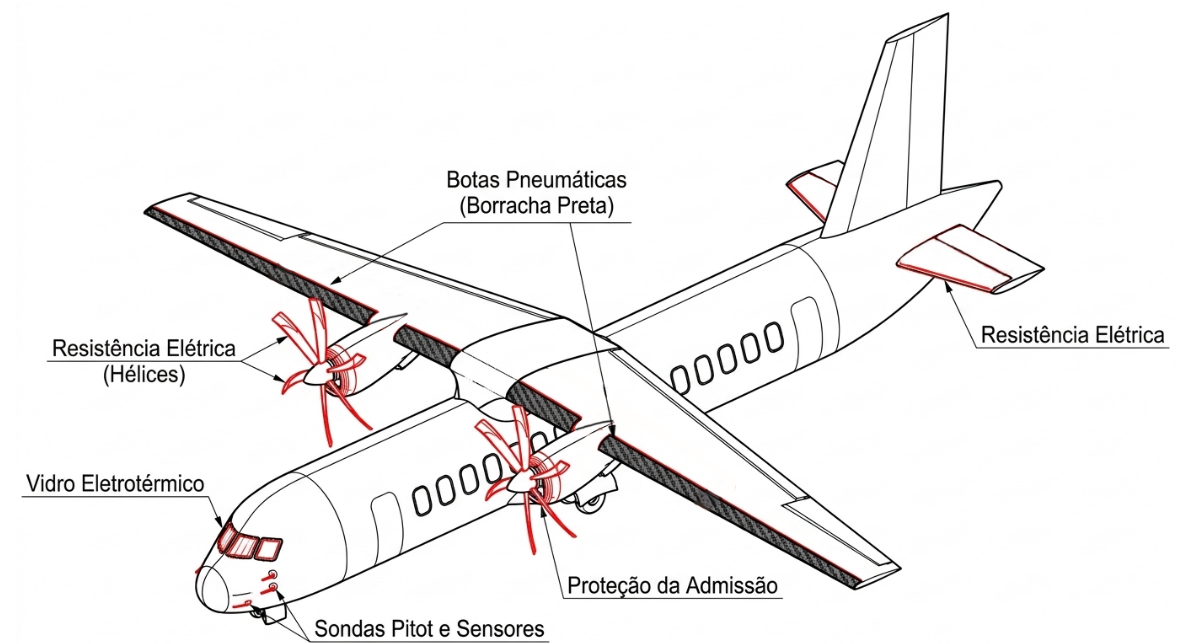
\includegraphics[width=1\textwidth]{images/Posicao sist degelo.png} 
    \caption{Posicionamento do sistema de Degelo na Aeronave}
    \label{fig:posicao_degelo}
\end{figure}
\chapter{Pesos e Centro de Gravidade}
Este capítulo é a única entrada de pesos e de posição do centro de gravidade do projeto. Os valores definidos aqui (Tabela~\ref{tab:cg_entradas}) são os que devem ser usados nos capítulos de Desempenho, Cargas, Dimensionamento Estrutural e Estabilidade, que vêm depois. O capítulo segue a sequência: estimativa de pesos e fechamento no peso máximo de decolagem; posição de cada item em relação ao datum; passeio e envelope do CG, com a verificação simplificada da margem estática; e verificação preliminar da posição do trem de pouso. A verificação completa de estabilidade, estática e dinâmica, é feita no Capítulo~\ref{estabilidade} com o envelope definido aqui.

\section{Estimativa de Pesos}
A fim de determinar o peso de cada componente da aeronave, é utilizada a metodologia apresentada em Roskam, 1985, aplicada à Classe II, Commercial Transports, Regional Turboprops, acima de 12500 lbs. As equações aqui referenciadas foram retiradas do livro em questão. Para isso, são utilizados os seguintes parâmetros de entrada, que foram obtidos, majoritariamente, da análise comparativa e da definição de requisitos:

\begin{table}[H]
  \centering
  \linespread{1}\small
  \setlength{\tabcolsep}{4pt}
  \caption{Parâmetros de Pesos e Fatores de Carga}
  \label{tab:pesos_cargas}
  \begin{tabularx}{\textwidth}{c >{\raggedright\arraybackslash}X c}
    \toprule
    \textbf{Parâmetro} & \textbf{Descrição} & \textbf{Valor} \\
    \midrule
    $W_{TO}$ & Peso Máximo de Decolagem & 50.000 lb \\
    $W_{L}$ & Peso Máximo de Pouso & 49.273 lb \\
    $W_{F,max}$ & Capacidade de Combustível (sistema de combustível) & 11.000 lb \\
    $W_{MZF}$ & Peso Máximo Zero Combustível (iterado, Seção~\ref{sec:cg_pesovazio}) & 43.193 lb \\
    $n_{ult}$ & Fator de Carga Última (Manobra) & 3,75 \\
    $n_{lim}$ & Fator de Carga Limite (Manobra) & 2,5 \\
    $n_{ult,l}$ & Fator de Carga Última de Pouso & 4,0 \\
    \bottomrule
  \end{tabularx}
\end{table}

\begin{table}[H]
  \centering
  \linespread{1}\small
  \setlength{\tabcolsep}{4pt}
  \caption{Parâmetros Geométricos e de Desempenho}
  \label{tab:geometricos_desempenho}
  \begin{tabularx}{\textwidth}{c >{\raggedright\arraybackslash}X c}
    \toprule
    \textbf{Parâmetro} & \textbf{Descrição} & \textbf{Valor} \\
    \midrule
    $S$ & Área Alar & 797,6 $ft^2$ \\
    $b$ & Envergadura & 93,5 ft \\
    $A$ & Aspect Ratio & 10,96 \\
    $t_r$ & Espessura Máxima da Raiz da Asa & 2,185 ft \\
    $\Lambda_{1/2}$ & Enflechamento de Meia Corda & 0 \\
    $l_f$ & Comprimento da Fuselagem & 85,3 ft \\
    $w_f + h_f$ & Largura + Altura da Fuselagem & 18,18 ft \\
    $V_D$ & Velocidade de Mergulho de Projeto & 250 kt \\
    $V_C$ & Velocidade de Cruzeiro de Projeto & 178,6 kt \\
    \bottomrule
  \end{tabularx}
\end{table}

\subsection{Peso Estrutural}
\paragraph{Asas ($W_w$)}

Utiliza-se o método de Torenbeek para aviões de transporte (Eq. 5.7), a qual pode ser vista na \autoref{eq:W_w}.

\begin{equation}
\label{eq:W_w}
\small
W_w = 0,0017 \, W_{MZF} \left( \frac{b}{\cos \Lambda_{1/2}} \right)^{0,75}
\left[ 1 + \left( \frac{6,3 \cos \Lambda_{1/2}}{b} \right)^{1/2} \right]
n_{ult}^{0,55}
\left( \frac{bS}{t_r W_{MZF} \cos \Lambda_{1/2}} \right)^{0,30}
\end{equation}

Sendo que $W_{MZF}$ é o peso máximo zero combustível com a cabine cheia, obtido por iteração na Seção~\ref{sec:cg_pesovazio}.

O peso obtido pela Equação~\ref{eq:W_w} corresponde a uma asa de referência e é corrigido conforme a configuração, de acordo com Torenbeek: $+2\%$ pelos flaps do tipo Fowler, cujos trilhos e atuadores acrescentam massa; $+2\%$ pelos spoilers; $-5\%$ pelos motores montados na asa, cujo peso alivia o momento fletor na raiz em voo; e $-5\%$ pelo trem de pouso principal montado na fuselagem, que dispensa reforços na asa para as cargas de pouso.

\paragraph{Empenagens ($W_h$, $W_v$)}

Para aeronaves com $V_D > 250$ kt, utilizam-se as Equações 5.19 (horizontal) e 5.20 (vertical).
\subparagraph{Estabilizador Horizontal}

Com $K_h = 1,0$, para estabilizador horizontal fixo.

\begin{equation}
W_h = K_h S_h \left[
\frac{3,81 \left( S_h^{0,2} V_D \right)}{1000 \sqrt{\cos \Lambda_{1/2}}}
- 0,287
\right]
\end{equation}

\subparagraph{Estabilizador Vertical}

Com $K_v = 1 + 0,15 \frac{S_h z_h}{S_v b_v}$, para cauda em T.

\begin{equation}
W_v = K_v S_v \left[
\frac{3,81 \left( S_v^{0,2} V_D \right)}{1000 \sqrt{\cos \Lambda_{1/2}}}
- 0,287
\right]
\end{equation}


\paragraph{Fuselagem ($W_f$)}

Peso estimado pela Equação 5.27 de Torenbeek, considerando fuselagem pressurizada, tem-se o $K_f = 1,08$.

\begin{equation}
W_f = 0,021 \, K_f \sqrt{\frac{V_D \, l_h}{w_f + h_f}} \, (S_{fgs})^{1,2}
\end{equation}


\paragraph{Nacelle ($W_n$)}

Para motores turboélice, o peso das nacelles é calculado pela Equação 5.33 de Roskam:

\begin{equation}
W_n = 0,14 \cdot P_{TO,total}
\end{equation}

Onde $P_{TO,total}$ é a potência total de decolagem em shp.


\paragraph{Trem de Pouso ($W_g$)}

Calculado pela Equação 5.42, com fator de asa alta, sendo $K_{gr} = 1,08$.

\begin{equation}
W_g = K_{gr} \left[
A_g + B_g W_{TO}^{3/4} + C_g W_{TO} + D_g W_{TO}^{3/2}
\right]
\end{equation}

\begin{table}[H]
  \centering
  \linespread{1}\small
  \setlength{\tabcolsep}{4pt}
  \caption{Constantes de Torenbeek para Trem de Pouso Retrátil na fuselagem}
  \label{tab:peso_trem_constantes}
  \begin{tabularx}{\textwidth}{>{\raggedright\arraybackslash}X c c c c}
    \toprule
    \textbf{Componente} & $A_g$ & $B_g$ & $C_g$ & $D_g$ \\
    \midrule
    \textbf{Principal (Main)} & 40,0 & 0,16 & 0,019 & $1,5 \times 10^{-5}$ \\
    \textbf{Nariz (Nose)} & 20,0 & 0,10 & 0,000 & $2,0 \times 10^{-6}$ \\
    \bottomrule
  \end{tabularx}
\end{table}

\subsection{Grupo Moto-Propulsor e Acessórios}

\paragraph{Motores}

Os motores a serem utilizados são o PW127M, cujo peso seco é 1060 lbs. (480,8 kg) para cada motor, conforme 05-10-00 Manual Part No. 3037332, Revision No. 51.0.

\paragraph{Sistema de Combustível}

Equação 6.24 para tanques integrais:

\begin{equation}
W_{fs} = 80(N_e + N_t - 1) + 15\sqrt{N_t} (W_F / K_{fsp})^{0,333}
\end{equation}

Em que, $K_{fsp}$ é a densidade do combustível QAV em lbs/gal.


\paragraph{Hélice}

De acordo com o manual de treinamento da Caribbean Airlines, o avião é equipado com duas hélices, e cada um desses sistemas pesa cerca de 159 kg (350 libras).

Essa hélice previamente escolhida foi a HAMILTON STANDARD 568F, que equipa as aeronaves ATR72-600.

\paragraph{Controladores}

Equação 6.25 para turbopropulsores na asa:

\begin{equation}
W_{ec} = 56,84 \left[ \frac{(l_f + b) N_e}{100} \right]^{0,514}
\end{equation}

\paragraph{Sistema de Partida}

Equação 6.30 para sistemas pneumáticos:

\begin{equation}
W_{ess} = 12,05 (W_{e,total} / 1.000)^{1,458}
\end{equation}


\subsection{Equipamentos Fixos}

\paragraph{Controles de Voo}

Calculado pela Equação 7.6 para aeronaves com controles de voo assistidos:

\begin{equation}
    W_{fc} = K_{fc} (W_{TO})^{2/3}
\end{equation}

onde $K_{fc} = 0,64$.

\paragraph{Sistema Hidráulico e Pneumático}

Conforme a metodologia adotada, o peso do sistema hidráulico e/ou pneumático necessário para os controles de voo assistidos já foi computado na previsão de peso do sistema de controle de voo.

\paragraph{Sistema Elétrico}

Estimado pela Equação 7.16:

\begin{equation}
    W_{els} = 0,325 (W_E)^{0,8}
\end{equation}

\paragraph{Aviônicos e Instrumentação}

Estimado inicialmente pela Equação 7.24:

\begin{equation}
    W_{iae} = 120 + 20N_e + 0,006W_{TO}
\end{equation}

A equação original é provavelmente muito conservadora, já que os sistemas aviônicos atuais são significativamente mais leves do que aqueles existentes quando a equação foi determinada. Para efeito de comparação, a Thales, fabricante dos aviônicos do ATR72, afirma que o Integrated Modular Avionics (IMA) reduz em até 40\% o peso do sistema. Esse valor foi considerado para redução do peso estimado.

\paragraph{Sistema de Pressurização e Ar-condicionado}

Para aeronaves pressurizadas, utiliza-se a Equação 7.30, baseada no comprimento da cabine de passageiros ($l_{pax}$):

\begin{equation}
    W_{api} = 6,75 (l_{pax})^{1,28}
\end{equation}

\paragraph{Sistema de Oxigênio}

Calculado pela Equação 7.36 para voos abaixo de 25.000 ft:

\begin{equation}
    W_{ox} = 20 + 0,5N_{pax}
\end{equation}


\paragraph{Mobiliário}

Peso do mobiliário interno estimado pela Equação 7.45:

\begin{equation}
    W_{fur} = 0,211 (W_{TO} - W_F)^{0,91}
\end{equation}

em que $W_{TO} - W_F$ é o peso zero combustível, tomado igual ao $W_{MZF}$ iterado na Seção~\ref{sec:cg_pesovazio}.

\paragraph{Equipamento para acomodação de carga e bagagem}

Estimado pela Equação 7.49, baseada na área do piso de carga ($S_{ff}$):

\begin{equation}
    W_{bc} = 3 S_{ff}
\end{equation}

\paragraph{Tinta}

Peso estimado pela Equação 7.51:

\begin{equation}
    W_{pt} = 0,003 W_{TO}
\end{equation}

\subsection{Resultados das Estimativas de Peso}
\begin{table}[H]
  \centering
  \linespread{1}\small
  \setlength{\tabcolsep}{4pt}
  \caption{Estimativa do peso vazio por componente (Classe II), com $W_{MZF}$ iterado.}
  \label{tab:oew_componentes}
  \begin{tabularx}{\textwidth}{>{\raggedright\arraybackslash}X r r}
    \toprule
    \textbf{Componente} & \textbf{Peso (lb)} & \textbf{Peso (kg)} \\
    \midrule
    \multicolumn{3}{l}{\textit{Grupo Estrutural}} \\
    Peso da Asa & 5033,82 & 2283,28 \\
    Estabilizador Horizontal & 495,46 & 224,74 \\
    Estabilizador Vertical & 464,60 & 210,74 \\
    Fuselagem & 8163,47 & 3702,88 \\
    Nacelle & 770,00 & 349,27 \\
    Trem de Pouso Principal & 1828,11 & 829,22 \\
    Trem de Pouso de Nariz & 406,87 & 184,55 \\
    \addlinespace
    \multicolumn{3}{l}{\textit{Grupo Moto-Propulsor}} \\
    Motores (PW127M) & 2120,00 & 961,62 \\
    Hélices & 700,00 & 317,51 \\
    Acessórios de Instalação & 127,20 & 57,70 \\
    Sistema de Combustível & 491,53 & 222,95 \\
    Controles do Motor (Wec) & 109,42 & 49,63 \\
    Sistema de Partida (Wess) & 36,04 & 16,35 \\
    \addlinespace
    \multicolumn{3}{l}{\textit{Grupo de Equipamentos Fixos}} \\
    Controles de Voo & 868,61 & 394,00 \\
    Aviônicos (IMA) & 276,00 & 125,19 \\
    Sistema Elétrico & 1500,00 & 680,39 \\
    Ar-cond./Pressurização/Degelo & 1356,62 & 615,35 \\
    Sistema de Oxigênio & 56,00 & 25,40 \\
    Mobiliário/Furnishings & 3487,48 & 1581,87 \\
    Equipamento de Carga/Bagagem & 360,00 & 163,29 \\
    Tinta & 150,00 & 68,04 \\
    \midrule
    \textbf{Peso vazio ($W_E$)} & \textbf{28801,24} & \textbf{13063,97} \\
    \bottomrule
  \end{tabularx}
\end{table}

\subsection{Peso vazio}
\label{sec:cg_pesovazio}
O peso vazio ($W_E$) é o somatório dos grupos estrutural, motopropulsor e de equipamentos fixos, estimados pelo método Classe~II nas seções anteriores. Duas dessas correlações dependem do peso zero combustível: a da asa, proporcional a $W_{MZF}^{0,70}$, e a do mobiliário, proporcional a $(W_{TO}-W_F)^{0,91}$, em que $W_{TO}-W_F$ é o próprio peso zero combustível. Na primeira avaliação, essas equações foram feitas com $W_F = 11\,000$ lb, que é a capacidade dos tanques, o que equivale a supor decolagem no MTOW com tanques cheios. Com 64 passageiros essa hipótese não se sustenta (Seção~\ref{sec:cg_fechamento}), e o valor de projeto passa a ser o MZFW da cabine cheia. Como o MZFW depende do peso vazio, as duas correlações são iteradas até a convergência:

\begin{equation}
W_{MZF}^{(k+1)} = W_E\!\left(W_{MZF}^{(k)}\right) + W_{trip} + W_{cat} + W_{CP},
\label{eq:cg_iteracao}
\end{equation}
em que $W_{trip}$ é a tripulação, $W_{cat}$ o catering e $W_{CP}$ a carga paga. A iteração converge em poucos passos e altera apenas dois itens: a asa, de 2\,125,8 para 2\,283,3 kgf, e o mobiliário, de 1\,441,5 para 1\,581,9 kgf. A Tabela~\ref{tab:oew_componentes} já apresenta os valores convergidos. Os demais itens não mudam, porque dependem do MTOW (fixo) ou da capacidade de combustível (fixa). O peso vazio resulta em $W_E = 13\,064$ kgf.

\subsection{Tripulação, passageiros e bagagem}
Adotam-se as massas-padrão da regulamentação de operações da EASA \cite{easa_airops}, já que o projeto usa a base normativa ANAC/FAA/EASA. Para aeronaves com 30 ou mais assentos, a norma admite 84 kg por passageiro adulto, com bagagem de mão incluída, e 11 kg por volume de bagagem despachada em voos domésticos. Para a tripulação, os valores são 85 kg por tripulante técnico e 75 kg por comissário, também com bagagem de mão. A Tabela~\ref{tab:cg_massas} resume os valores.

\begin{table}[H]
  \centering
  \linespread{1}\small
  \setlength{\tabcolsep}{4pt}
  \caption{Massas-padrão adotadas para pessoas e bagagem \cite{easa_airops}.}
  \label{tab:cg_massas}
  \begin{tabularx}{\textwidth}{>{\raggedright\arraybackslash}X c c c}
    \toprule
    \textbf{Item} & \textbf{Quantidade} & \textbf{Massa unitária [kgf]} & \textbf{Total [kgf]} \\
    \midrule
    Pilotos & 2 & 85 & 170 \\
    Comissários & 2 & 75 & 150 \\
    Passageiros (com bagagem de mão) & 64 & 84 & 5\,376 \\
    Bagagem despachada (doméstico) & 64 & 11 & 704 \\
    \bottomrule
  \end{tabularx}
\end{table}

\subsection{Fechamento no peso máximo de decolagem}
\label{sec:cg_fechamento}
O MTOW de 50\,000 lb (22\,680 kgf) é requisito de projeto e não é ultrapassado. Ele é composto pelo peso vazio operacional (OEW), pela carga paga e pelo combustível. O OEW inclui a tripulação e o catering, que estão a bordo em qualquer voo. Com a cabine cheia, o combustível disponível é o que falta para chegar ao MTOW:

\begin{equation}
W_{F} = MTOW - MZFW = 22\,680 - 19\,592 = 3\,088 \ \text{kgf}.
\label{eq:cg_combustivel}
\end{equation}

\begin{table}[H]
  \centering
  \linespread{1}\small
  \setlength{\tabcolsep}{4pt}
  \caption{Composição dos pesos da aeronave (configuração de passageiros).}
  \label{tab:cg_pesos}
  \begin{tabularx}{\textwidth}{>{\raggedright\arraybackslash}X r}
    \toprule
    \textbf{Parcela} & \textbf{Peso [kgf]} \\
    \midrule
    Peso vazio, $W_E$ (Classe II, iterado) & 13\,064 \\
    Tripulação (2 pilotos + 2 comissários) & 320 \\
    \emph{Catering} / \emph{galley} & 128 \\
    \textbf{Peso vazio operacional (OEW)} & \textbf{13\,512} \\
    Passageiros (64) & 5\,376 \\
    Bagagem despachada & 704 \\
    \textbf{Peso máximo zero combustível (MZFW)} & \textbf{19\,592} \\
    Combustível com carga paga máxima & 3\,088 \\
    \textbf{Peso máximo de decolagem (MTOW)} & \textbf{22\,680} \\
    \bottomrule
  \end{tabularx}
\end{table}

A capacidade dos tanques continua sendo de 4\,990 kgf. Ela só pode ser usada inteira com carga paga reduzida, como em qualquer aeronave de transporte. A Tabela~\ref{tab:cg_cargapaga} mostra os dois pontos que limitam o diagrama carga paga--alcance.


\begin{table}[H]
  \centering
  \linespread{1}\small
  \setlength{\tabcolsep}{4pt}
  \caption{Pontos limite de carga paga e combustível no MTOW.}
  \label{tab:cg_cargapaga}
  \begin{tabularx}{\textwidth}{>{\raggedright\arraybackslash}X c c c}
    \toprule
    \textbf{Condição} & \textbf{Carga paga [kgf]} & \textbf{Combustível [kgf]} & \textbf{Limitada por} \\
    \midrule
    Carga paga máxima & 6\,080 & 3\,088 & MZFW e MTOW \\
    Combustível máximo & 4\,178 & 4\,990 & Tanques e MTOW \\
    \bottomrule
  \end{tabularx}
\end{table}

O ATR~72-600, de MTOW e grupo motopropulsor semelhantes, serve de verificação de ordem de grandeza \cite{atr72600}, com OEW típico em serviço de 13\,600 kg, contra 13\,512 kgf aqui. Com MTOW de 23\,000 kg e 70 passageiros de 95 kg, seu alcance com passageiros máximos é de 740 NM, com reservas EASA e alternativa a 100 NM, o que corresponde a cerca de 2\,750 kg de combustível. Os 3\,088 kgf disponíveis aqui, para 800 NM com 64 passageiros, estão na mesma ordem de grandeza. O peso máximo de pouso de 22\,350 kgf é respeitado em qualquer pouso realizado após o consumo de mais de 330 kgf de combustível.

\section{Datum e Posição dos Itens}
\label{sec:cg_posicoes}
O datum é a ponta do nariz da fuselagem, com o eixo $x$ positivo em direção à cauda. É o mesmo referencial dos desenhos. A Figura~\ref{fig:cg_esquema} mostra a posição de todos os itens de peso sobre a vista lateral, com o datum, a CMA e a faixa de CG admissível. A numeração da figura é a da Tabela~\ref{tab:cg_bracos}.


\begin{figure}[H]
\centering
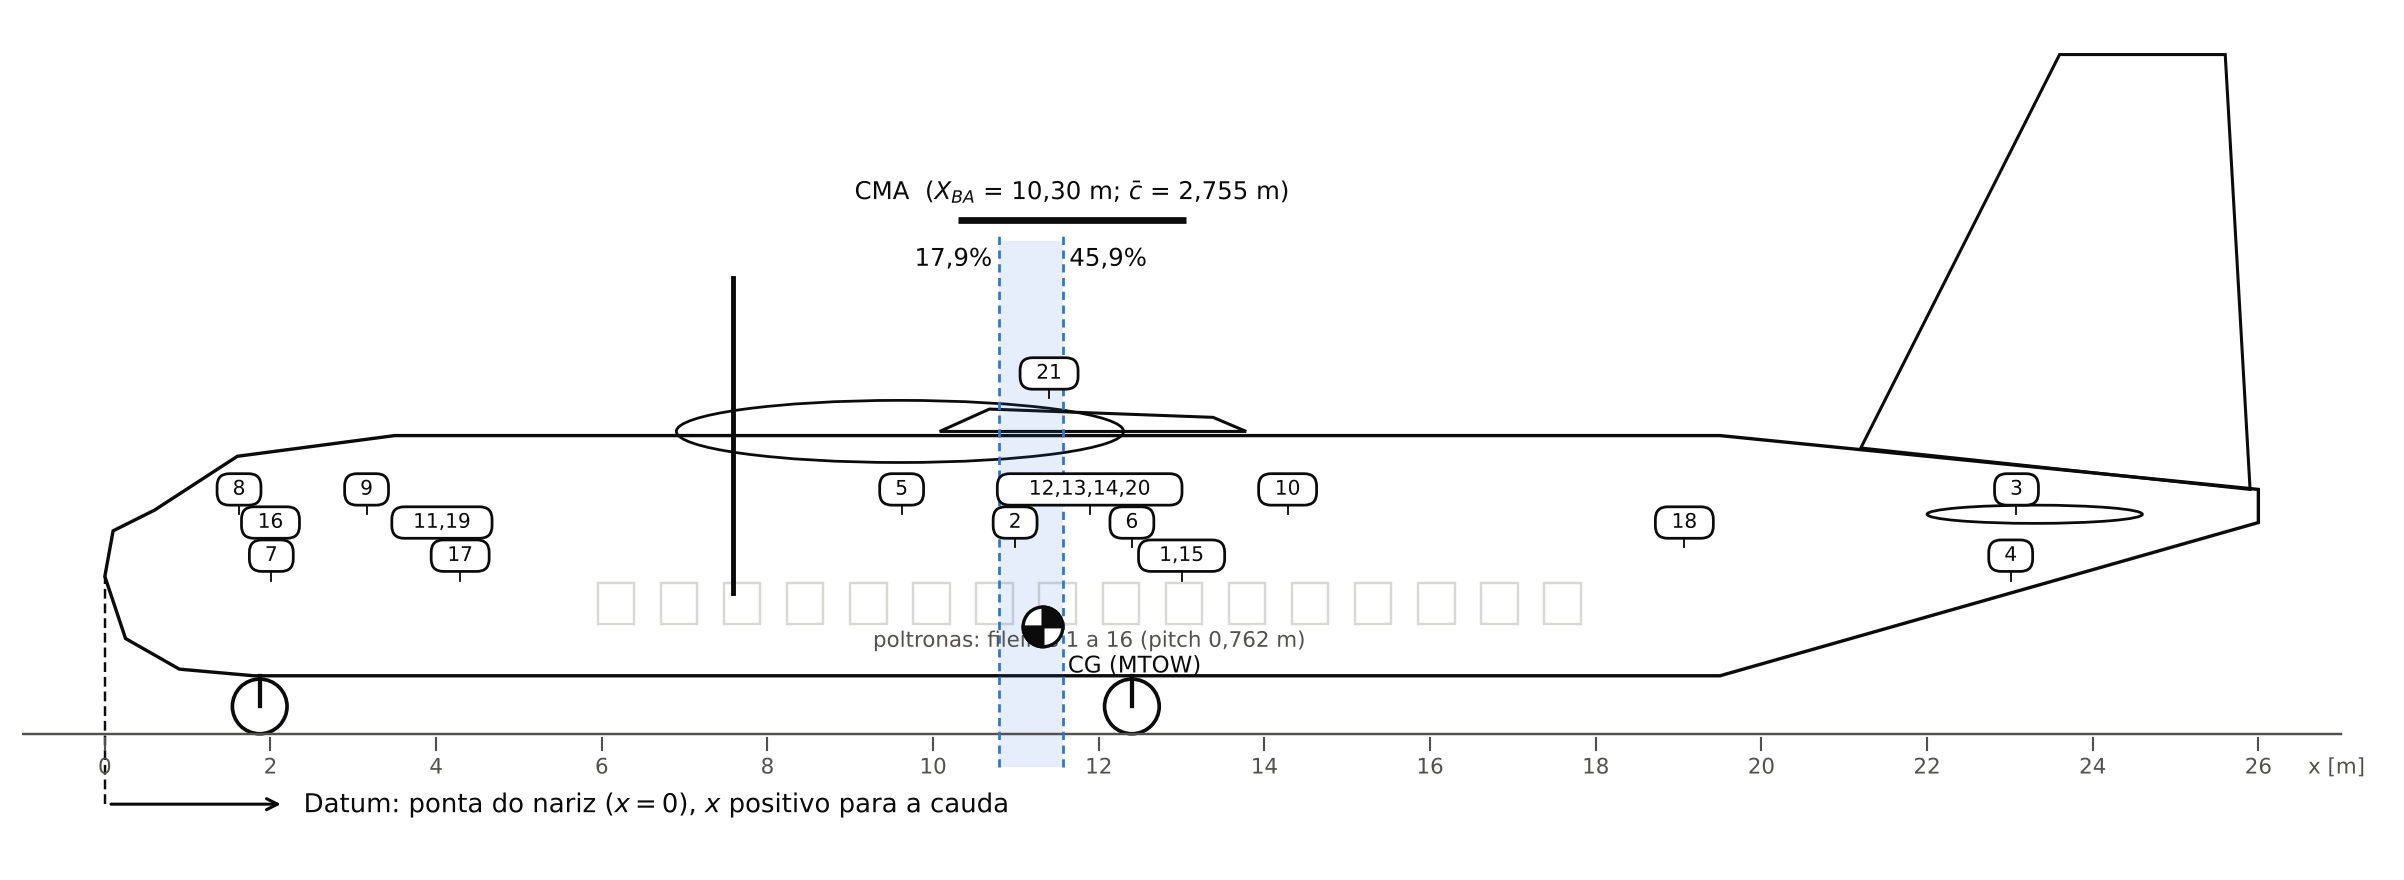
\includegraphics[width=\textwidth]{Images-CG/cg_esquema_lateral.png}
\caption{Diagrama esquemático da vista lateral com a posição dos itens de peso, o datum, a CMA e a faixa de CG admissível.}
\label{fig:cg_esquema}
\end{figure}

\begin{figure}[H]
\centering
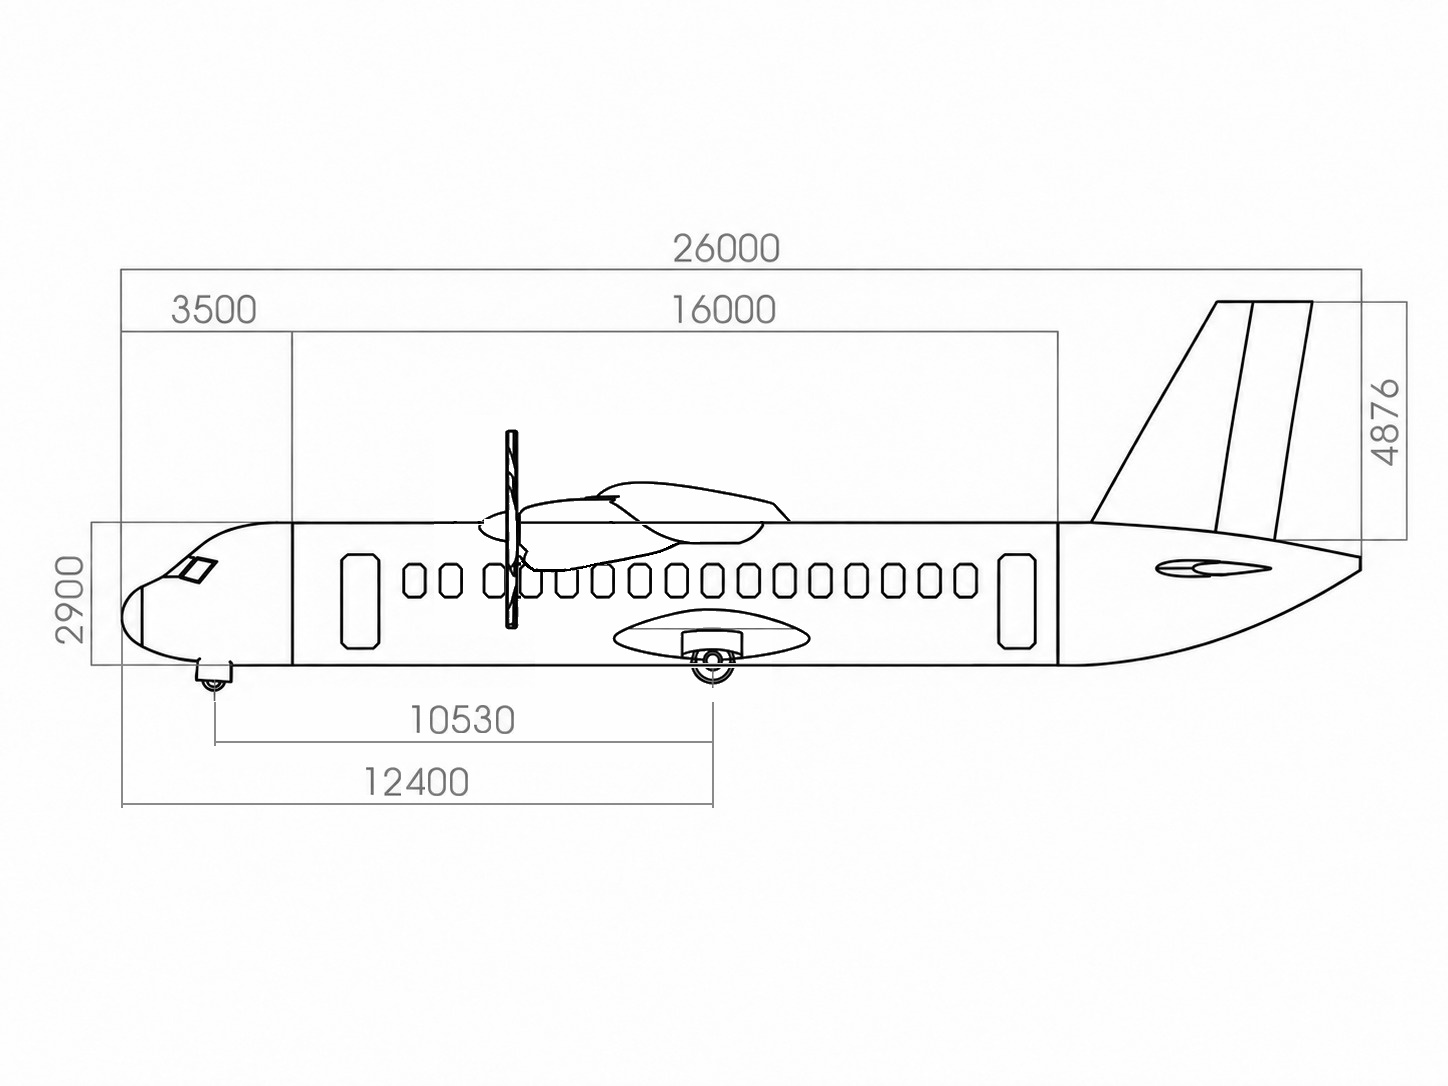
\includegraphics[width=0.85\textwidth]{Images-CG/VistaLateral.jpeg}
\caption{Vista lateral com cotas usada como referência geométrica.}
\label{fig:cg_vista_ref}
\end{figure}

\subsection{Posição da asa}

A posição da asa é definida pelo bordo de ataque da CMA, $X_{BA,\text{CMA}} = 10{,}30$ m, com $\bar{c} = 2{,}755$ m. Essa é a posição em que o braço da empenagem horizontal ($l_{EH} = 12{,}0$ m) e o volume de cauda ($\bar{V}_{HT} = 1{,}1$) da Conclusão do Anteprojeto (Tabela~\ref{tab:dimensoes_conclusao}) são consistentes: o centro aerodinâmico da asa fica em 10,99 m e o da empenagem em 22,99 m, junto ao braço de 23,08 m da empenagem horizontal.

Os itens presos à asa acompanham sua posição. O O CG da asa mantém a posição relativa adotada no anteprojeto, a 25\% da CMA (0,686 m atrás do bordo de ataque) O combustível, nos tanques integrais, é posicionado a 40\% da CMA (11,40 m).

O braço do grupo motopropulsor foi estimado pelos seus subcomponentes, com as distâncias ao bordo de ataque da CMA medidas na vista lateral (Tabela~\ref{tab:cg_gmp}). O resultado coloca o conjunto 0,68 m à frente do bordo de ataque da CMA, coerente com motores montados à frente da asa.

\begin{table}[H]
  \centering
  \linespread{1}\small
  \setlength{\tabcolsep}{4pt}
  \caption{Estimativa do braço do grupo motopropulsor por subcomponentes (distâncias ao bordo de ataque da CMA).}
  \label{tab:cg_gmp}
  \begin{tabularx}{\textwidth}{>{\raggedright\arraybackslash}X c c c}
    \toprule
    \textbf{Subcomponente} & \textbf{Peso [kgf]} & \textbf{Distância ao BA da CMA [m]} & \textbf{Referência} \\
    \midrule
    Hélices (2) & 317,5 & $-2{,}14$ & Plano do disco \\
    Motores PW127M (2) & 961,6 & $-1{,}02$ & Centro do motor \\
    Acessórios, controles e partida & 123,7 & $-1{,}02$ & Junto ao motor \\
    Naceles & 349,3 & $+0{,}58$ & Centroide da nacele \\
    Sistema de combustível & 223,0 & $+1{,}10$ & 40\% da CMA \\
    \midrule
    \textbf{Grupo motopropulsor} & \textbf{1\,975,0} & $\mathbf{-0{,}68}$ & $x = 9{,}62$ m \\
    \bottomrule
  \end{tabularx}
\end{table}

\subsection{Itens fixos à fuselagem}

As empenagens e o trem de nariz têm braço obtido da geometria do desenho. A fuselagem é posicionada a 50\% do seu comprimento (13,00 m), hipótese usual para uma estrutura de seção aproximadamente constante. Comandos de voo, aviônicos, equipamento de carga e o sistema de ar-condicionado e pressurização são posicionados conforme o arranjo interno: os comandos no posto de pilotagem (1,62 m), os aviônicos na baia logo atrás da cabine de comando (3,16 m), o equipamento de carga no compartimento de bagagem dianteiro (4,07 m) e os packs de ar-condicionado em um compartimento ventral não pressurizado logo atrás da raiz da asa (14,28 m), como em aeronaves da mesma classe. O item de ar-condicionado da Classe~II de Roskam engloba também a proteção contra gelo, de modo que os 120 kgf do sistema de degelo estão contidos nos 615,4 kgf desse item. Os sistemas elétrico e de oxigênio e o mobiliário, que se distribuem ao longo da cabine, são posicionados no centroide das 16 fileiras de passageiros (11,89 m). A tinta é posicionada no centroide da fuselagem (13,00 m).

\begin{table}[H]
  \centering
  \linespread{1}\small
  \setlength{\tabcolsep}{4pt}
  \caption{Pesos, braços e momentos do peso vazio e do peso vazio operacional ($X_{BA,\text{CMA}} = 10{,}30$ m; trem principal em 12,40 m).}
  \label{tab:cg_bracos}
  \begin{tabularx}{\textwidth}{c >{\raggedright\arraybackslash}X r r r >{\raggedright\arraybackslash}X}
    \toprule
    \textbf{N.º} & \textbf{Item} & \textbf{Peso [kgf]} & \textbf{Braço [m]} & \textbf{Momento [kgf$\cdot$m]} & \textbf{Origem do braço} \\
    \midrule
    1 & Fuselagem & 3\,702,9 & 13,00 & 48\,137 & Hipótese: 50\% de $l_f$ \\
    2 & Asa & 2\,283,3 & 10,99 & 25\,084 & 25\% da CMA \\
    3 & Empenagem horizontal & 224,7 & 23,08 & 5\,187 & Desenho \\
    4 & Empenagem vertical & 210,7 & 23,01 & 4\,849 & Desenho \\
    5 & Grupo motopropulsor & 1\,974,9 & 9,62 & 18\,999 & Tabela~\ref{tab:cg_gmp} \\
    6 & Trem de pouso principal & 829,2 & 12,40 & 10\,282 & Seção~\ref{sec:cg_trem} \\
    7 & Trem de pouso de nariz & 184,6 & 2,01 & 371 & Desenho \\
    8 & Comandos de voo & 394,0 & 1,62 & 638 & Posto de pilotagem \\
    9 & Aviônicos & 125,2 & 3,16 & 396 & Baia de aviônicos \\
    10 & Ar-cond., pressurização e degelo & 615,4 & 14,28 & 8\,787 & Compartimento ventral \\
    11 & Equip. de carga e bagagem & 163,3 & 4,07 & 665 & Compartimento dianteiro \\
    12 & Sistema elétrico & 680,4 & 11,89 & 8\,088 & Centroide da cabine \\
    13 & Sistema de oxigênio & 25,4 & 11,89 & 302 & Centroide da cabine \\
    14 & Mobiliário & 1\,581,9 & 11,89 & 18\,805 & Centroide da cabine \\
    15 & Tinta & 68,0 & 13,00 & 885 & Centroide da fuselagem \\
    \midrule
     & \textbf{Peso vazio, $W_E$} & \textbf{13\,063,9} & \textbf{11,59} & \textbf{151\,475} & \\
    \midrule
    16 & Pilotos (2 × 85 kgf) & 170,0 & 2,00 & 340 & Cabine de comando \\
    17 & Comissários (2 × 75 kgf) & 150,0 & 4,29 & 644 & Assentos de comissário \\
    18 & \emph{Catering} / \emph{galley} & 128,0 & 19,07 & 2\,441 & \emph{Galley} traseira \\
    \midrule
     & \textbf{Peso vazio operacional, OEW} & \textbf{13\,511,9} & \textbf{11,46} & \textbf{154\,900} & \\
    \midrule
    19 & Bagagem despachada & 704,0 & 4,07 & 2\,865 & Compartimento dianteiro \\
    20 & Passageiros (centroide) & 5\,376,0 & 11,89 & 63\,909 & Fileiras 1 a 16 \\
    21 & Combustível com carga paga máxima & 3\,088,0 & 11,40 & 35\,209 & 40\% da CMA \\
    \bottomrule
  \end{tabularx}
\end{table}

O CG em porcentagem da CMA é obtido por
\begin{equation}
\bar{X}_{CG} = \frac{\sum W_i x_i}{\sum W_i}, \qquad
h_{CG} = \frac{\bar{X}_{CG} - X_{BA,\text{CMA}}}{\bar{c}} \times 100\%.
\label{eq:cg}
\end{equation}

\section{Passeio e Envelope do CG}
\label{sec:cg_envelope}

\subsection{Condições de carregamento}

A partir do OEW, a carga útil é somada item a item e o CG é recalculado a cada passo. A bagagem despachada é carregada primeiro, no compartimento dianteiro. Os passageiros embarcam em grupos de quatro fileiras, em duas sequências: da frente para trás e de trás para a frente. Essas sequências limitam o passeio, já que qualquer outra ordem de embarque produz posições entre elas. As mesmas sequências são repetidas sem bagagem despachada, caso em que o CG fica mais traseiro. O combustível, a 40\% da CMA, aproxima o CG dessa posição. Por isso as condições sem combustível, que também representam o pouso com reserva mínima, são as mais extremas. A Tabela~\ref{tab:cg_passeio} e a Figura~\ref{fig:cg_envelope} apresentam os resultados.

\begin{table}[H]
  \centering
  \linespread{1}\small
  \setlength{\tabcolsep}{4pt}
  \caption{Passeio do CG por condição de carregamento ($X_{BA,\text{CMA}} = 10{,}30$ m; $\bar{c} = 2{,}755$ m).}
  \label{tab:cg_passeio}
  \begin{tabularx}{\textwidth}{>{\raggedright\arraybackslash}X c c c}
    \toprule
    \textbf{Condição} & \textbf{Peso [kgf]} & $\bar{X}_{CG}$ \textbf{[m]} & $h_{CG}$ \textbf{[\% CMA]} \\
    \midrule
    OEW & 13\,512 & 11,46 & 42,2 \\
    OEW + bagagem & 14\,216 & 11,10 & 29,0 \\
    \multicolumn{4}{l}{\textit{Embarque da frente para trás (com bagagem)}} \\
    \quad fileiras 1--4 & 15\,560 & 10,77 & 17,1 \\
    \quad fileiras 1--8 & 16\,904 & 10,74 & 15,9 \\
    \quad fileiras 1--12 & 18\,248 & 10,94 & 23,1 \\
    \multicolumn{4}{l}{\textit{Embarque de trás para a frente (com bagagem)}} \\
    \quad fileiras 13--16 & 15\,560 & 11,56 & 45,8 \\
    \quad fileiras 9--16 & 16\,904 & 11,71 & 51,1 \\
    \quad fileiras 5--16 & 18\,248 & 11,61 & 47,5 \\
    MZFW (cabine cheia, com bagagem) & 19\,592 & 11,32 & 36,8 \\
    MTOW (cabine cheia, 3\,088 kgf de combustível) & 22\,680 & 11,33 & 37,3 \\
    Cabine cheia, sem bagagem, sem combustível & 18\,888 & 11,58 & 46,6 \\
    \bottomrule
  \end{tabularx}
\end{table}

\begin{figure}[H]
\centering
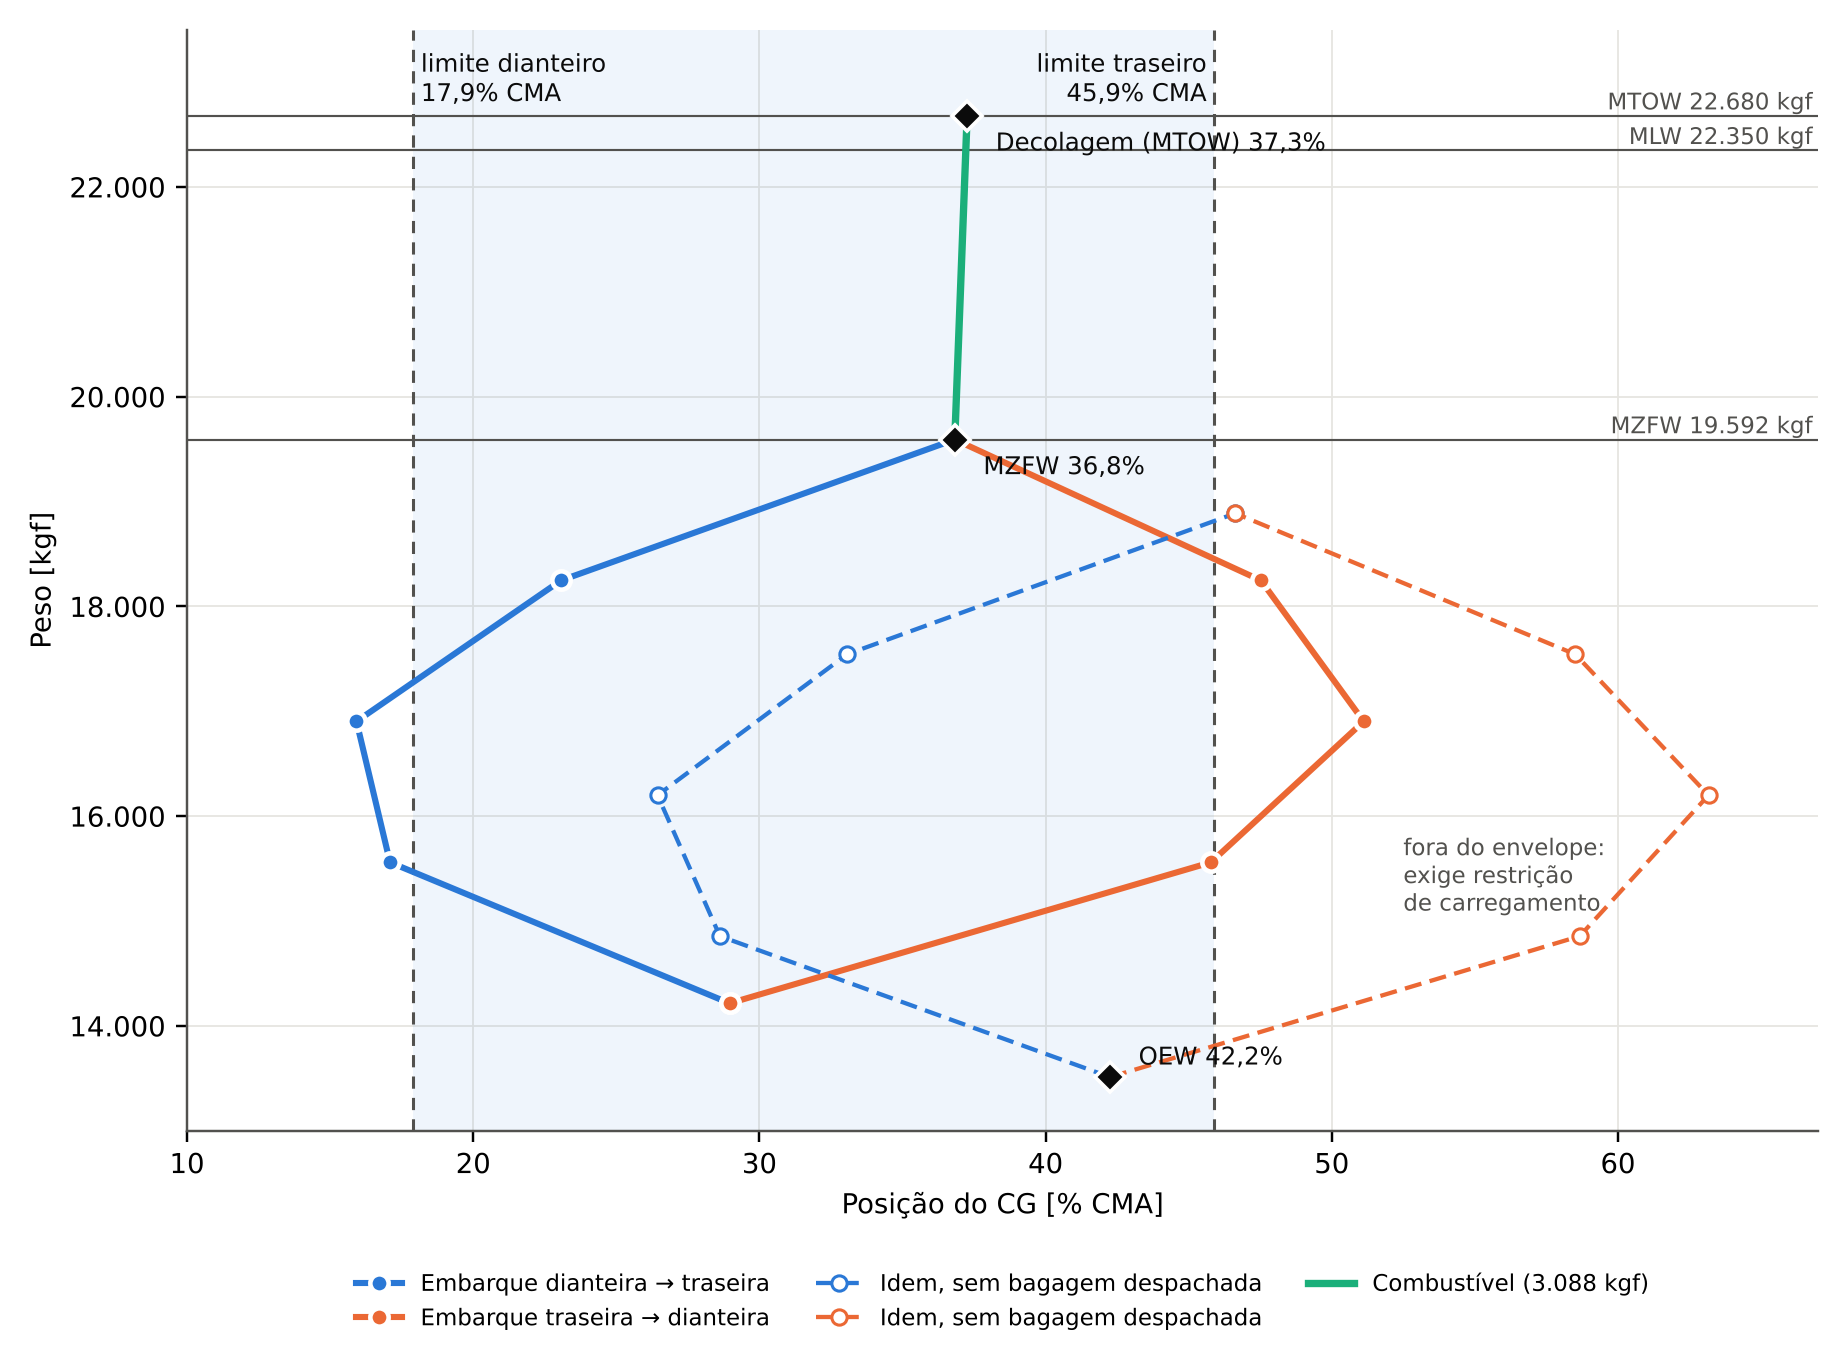
\includegraphics[width=0.92\textwidth]{Images-CG/cg_envelope.png}
\caption{Envelope de CG para o operador: limites de CG, pesos limite e linhas de carregamento. Linhas cheias com bagagem despachada; tracejadas sem bagagem despachada.}
\label{fig:cg_envelope}
\end{figure}

\subsection{Limites de CG e verificação simplificada da margem estática}
\label{sec:cg_margem}

Os limites de CG propostos são 17,9\% da CMA (dianteiro) e 45,9\% da CMA (traseiro), ou seja, $\bar{X}_{CG}$ entre 10,79 m e 11,56 m. As condições de cabine cheia (MZFW, MTOW e pouso) ficam entre 36,8\% e 37,3\% da CMA, longe dos dois limites. O OEW, a 42,2\%, também está dentro deles.

A verificação simplificada usa a margem estática $ME = h_n - h_{CG}$, com o ponto neutro estimado pela contribuição da asa e da empenagem horizontal \cite{raymer2018}:
\begin{equation}
h_n = h_{ca} + \eta_h \, \bar{V}_{HT} \, \frac{a_h}{a_w}\left(1 - \frac{d\varepsilon}{d\alpha}\right).
\label{eq:cg_ponto_neutro}
\end{equation}
Com $h_{ca} = 0{,}25$, $\eta_h = 0{,}9$, $\bar{V}_{HT} = 1{,}098$, $a_w = 5{,}24$ rad$^{-1}$ ($A = 10{,}96$), $a_h = 3{,}77$ rad$^{-1}$ ($A_h = 3{,}76$) e $d\varepsilon/d\alpha = 2a_w/(\pi A) = 0{,}30$, obtém-se $h_n = 0{,}745$. As inclinações das curvas de sustentação foram estimadas pela fórmula de Helmbold para asa sem enflechamento. O AVL, no Capítulo~\ref{estabilidade}, fornece $h_n = 0{,}766$, valor próximo deste. A margem estática resulta em 56,6\% no limite dianteiro e 28,6\% no limite traseiro, positiva em todo o envelope.

A equação~\eqref{eq:cg_ponto_neutro} não inclui o efeito desestabilizante da fuselagem, que desloca o ponto neutro para a frente. Mesmo com uma redução de 0,15$\bar{c}$ por esse efeito, a margem no limite traseiro continuaria positiva, próxima de 14\%. As margens elevadas refletem o volume de cauda de 1,1. O efeito na força de profundor na rotação e no arrasto de compensação, bem como a verificação do limite dianteiro, são tratados no Capítulo~\ref{estabilidade}.

\textbf{Precisa deslocar a asa?} Não, além do deslocamento de 0,58 m para trás já adotado. Na posição do anteprojeto e do desenho atual ($X_{BA,\text{CMA}} = 9{,}72$ m), com os braços corrigidos, o OEW ficaria a 56,7\% da CMA, o MZFW a 53,3\% e o carregamento mais traseiro a 78,7\%, praticamente sobre o ponto neutro. Com $X_{BA,\text{CMA}} = 10{,}30$ m, as condições de cabine cheia ficam no centro do envelope. Os desenhos de três vistas devem ser atualizados para essa posição de asa.

\subsection{Restrições de carregamento para o operador}
\label{sec:cg_operador}

O envelope de CG é usado pelo operador e pelo despacho para definir como a aeronave pode ser carregada. As condições da Tabela~\ref{tab:cg_passeio} que ficam fora dos limites são de ocupação parcial concentrada em uma das metades da cabine. Elas definem as regras abaixo.

\begin{table}[H]
  \centering
  \linespread{1}\small
  \setlength{\tabcolsep}{4pt}
  \caption{Faixa admissível do centroide dos passageiros, sem combustível (caso crítico). Fileira 1 em 6,17 m; \emph{pitch} de 0,762 m.}
  \label{tab:cg_operador}
  \begin{tabularx}{\textwidth}{c >{\raggedright\arraybackslash}X >{\raggedright\arraybackslash}X}
    \toprule
    \textbf{Passageiros} & \textbf{Com bagagem despachada} & \textbf{Sem bagagem despachada} \\
    \midrule
    16 & até 13,56 m (fileira 10) & até 12,58 m (fileira 9) \\
    32 & 8,30 a 13,05 m (fileiras 4 a 10) & 7,42 a 12,07 m (fileiras 3 a 8) \\
    48 & 9,43 a 12,88 m (fileiras 5 a 9) & 8,55 a 11,90 m (fileiras 4 a 8) \\
    64 & 9,99 a 12,80 m (fileiras 6 a 9) & 9,11 a 11,82 m (fileiras 5 a 8) \\
    \bottomrule
  \end{tabularx}
\end{table}

\begin{itemize}
    \item \textbf{Ocupação parcial:} distribuir os passageiros a partir das fileiras centrais, de modo que o centroide fique entre as fileiras 6 e 8. Essa faixa atende a todas as condições da Tabela~\ref{tab:cg_operador}. Não ocupar apenas a metade dianteira ou apenas a metade traseira da cabine.
    \item \textbf{Cabine cheia sem bagagem despachada:} o CG sem combustível fica em 46,6\%, 0,7 ponto à ré do limite. Basta carregar pelo menos 60 kgf (bagagem, carga ou lastro) no compartimento dianteiro.
    \item \textbf{Configuração cargueira:} sem comissários e \emph{catering}, o OEW é de 13\,234 kgf a 42,5\% da CMA. O centroide da carga deve ficar entre 9,3 e 11,8 m do nariz para 6\,080 kgf, entre 8,5 e 11,9 m para 4\,000 kgf e entre 6,3 e 12,2 m para 2\,000 kgf. Essas faixas devem constar do manual de carregamento e definem as posições de batente e de fixação nos trilhos do piso.
\end{itemize}

\section{Verificação Preliminar do Trem de Pouso}
\label{sec:cg_trem}

A posição longitudinal do trem principal é verificada pelos dois critérios de Raymer \cite{raymer2018}, aplicados aos limites de CG da Seção~\ref{sec:cg_margem}:
\begin{itemize}
    \item ângulo de \emph{tip-back}, entre a vertical do CG e a linha que liga o CG ao contato do trem principal, de pelo menos 15° no CG traseiro;
    \item fração do peso no trem de nariz entre 8\% e 15\%, com faixa admissível de 5\% a 20\%, nos extremos traseiro e dianteiro.
\end{itemize}
A altura do CG em relação ao solo é $h_{CG} = 0{,}70 + 0{,}59 = 1{,}29$ m, soma da altura do trem e da altura do CG acima do ponto mais baixo da fuselagem. O trem de nariz permanece em 1,87 m. A fração no nariz e o ângulo de \emph{tip-back} são
\begin{equation}
\frac{N}{W} = \frac{x_{TP} - \bar{X}_{CG}}{x_{TP} - x_{TN}}, \qquad
\theta_{tb} = \arctan\frac{x_{TP} - \bar{X}_{CG}}{h_{CG}}.
\label{eq:cg_trem}
\end{equation}

Na posição anterior ($x_{TP} = 10{,}87$ m), o CG fica atrás do trem principal em toda condição acima de 20,7\% da CMA, o que inclui a cabine cheia: a aeronave apoiaria a cauda no solo. Impondo os critérios aos limites de CG:
\begin{itemize}
    \item \emph{tip-back} $\geq 15^\circ$ no limite traseiro: $x_{TP} \geq 11{,}91$ m;
    \item nariz $\geq 5\%$ no limite traseiro: $x_{TP} \geq 12{,}07$ m (para $\geq 8\%$: $x_{TP} \geq 12{,}41$ m);
    \item nariz $\leq 20\%$ no limite dianteiro: $x_{TP} \leq 13{,}02$ m (para $\leq 15\%$: $x_{TP} \leq 12{,}37$ m).
\end{itemize}
A faixa preferencial de 8\% a 15\% não tem solução, por 4 cm, porque a excursão do CG (0,77 m) ocupa quase toda a variação de fração admitida pela base de rodas. Adota-se $x_{TP} = 12{,}40$ m, dentro da faixa ampliada e a 1 cm do limite preferencial traseiro. A base de rodas passa a ser de 10,53 m.

\begin{figure}[H]
\centering
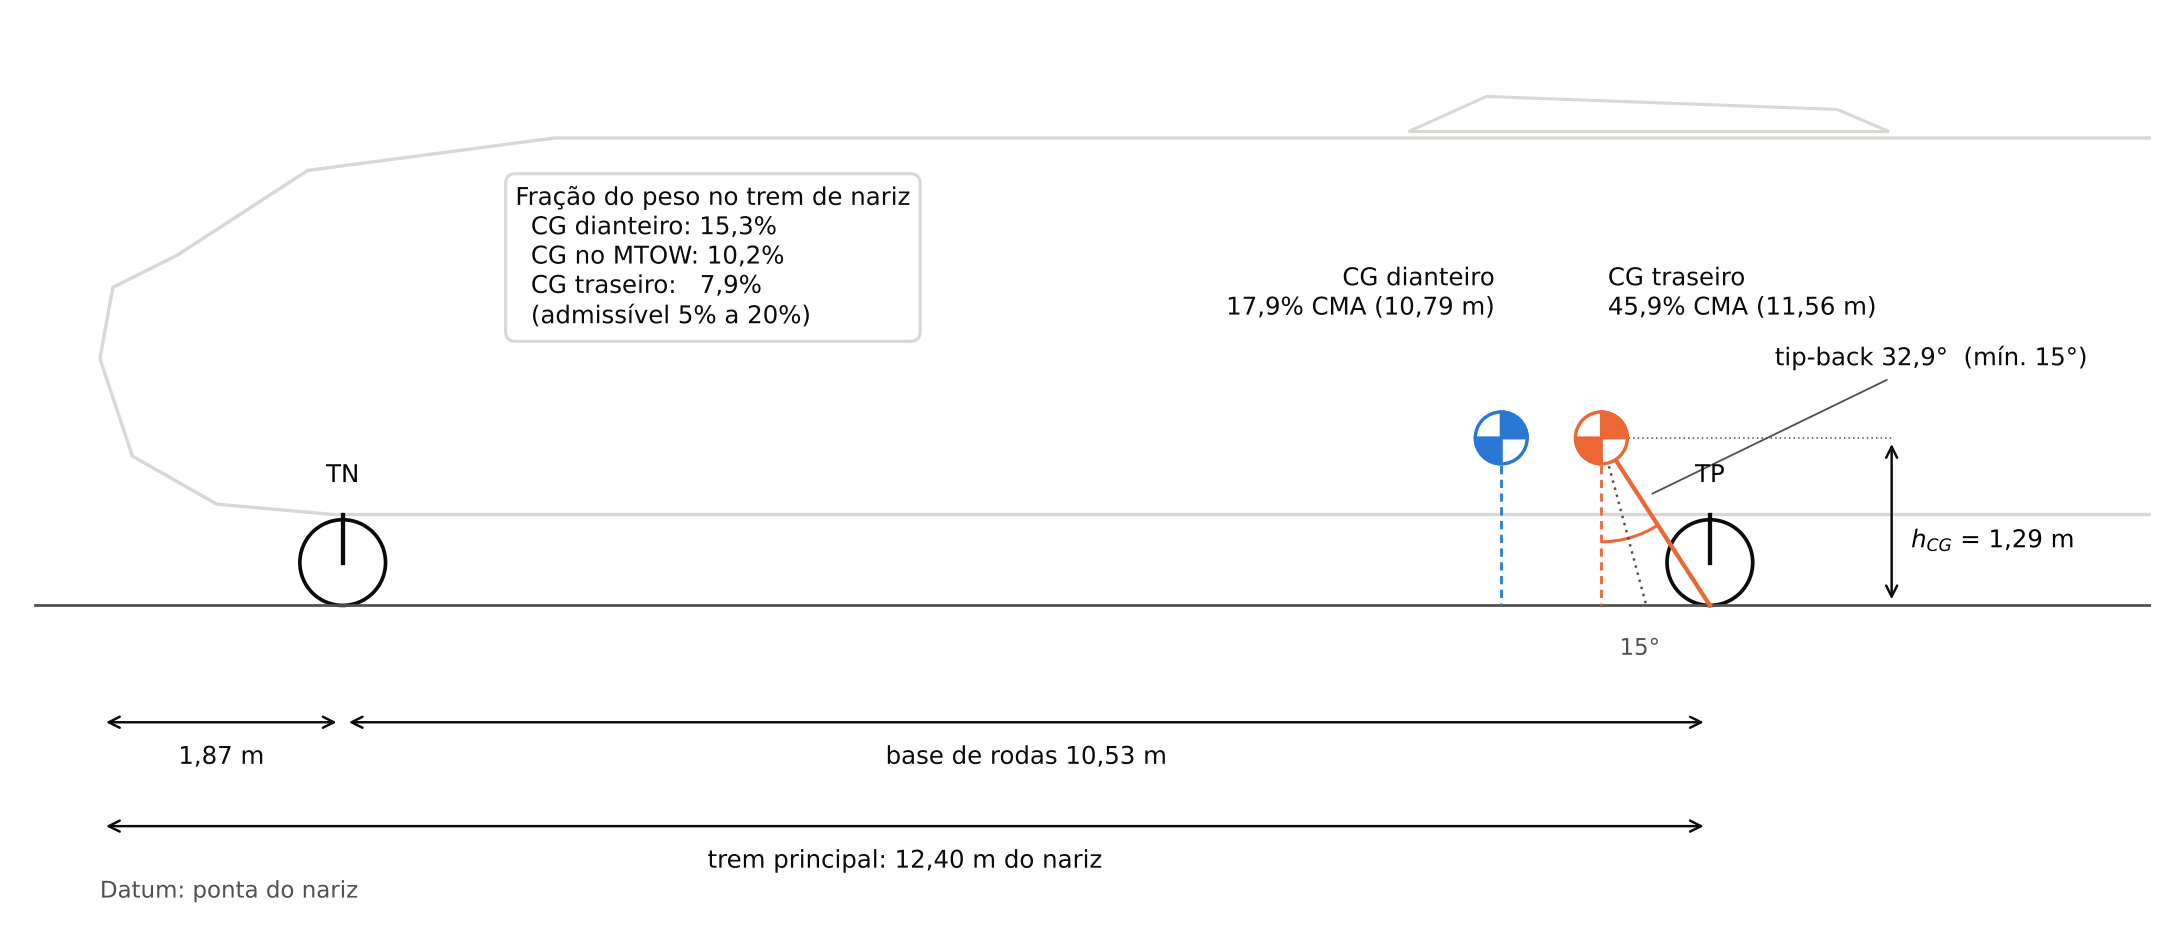
\includegraphics[width=\textwidth]{Images-CG/cg_trem_posicionamento.png}
\caption{Posicionamento longitudinal do trem de pouso em relação aos limites de CG.}
\label{fig:cg_trem}
\end{figure}

\begin{table}[H]
  \centering
  \linespread{1}\small
  \setlength{\tabcolsep}{4pt}
  \caption{Verificação do trem com o trem principal em 12,40 m e o trem de nariz em 1,87 m (cargas estáticas no MTOW).}
  \label{tab:cg_trem}
  \begin{tabularx}{\textwidth}{>{\raggedright\arraybackslash}X c c c c c c}
    \toprule
    \textbf{Condição} & $\bar{X}_{CG}$ \textbf{[m]} & $x_m$ \textbf{[m]} & $x_n$ \textbf{[m]} & \textbf{Tip-back} & \textbf{Nariz} & \textbf{Carga TP / TN [kgf]} \\
    \midrule
    Limite dianteiro (17,9\%) & 10,79 & 1,607 & 8,923 & 51,2° & 15,3\% & 19\,219 / 3\,461 \\
    CG no MTOW (37,3\%) & 11,33 & 1,074 & 9,456 & 39,8° & 10,2\% & 20\,368 / 2\,312 \\
    Limite traseiro (45,9\%) & 11,56 & 0,835 & 9,695 & 32,9° & 7,9\% & 20\,881 / 1\,799 \\
    \midrule
    \multicolumn{4}{l}{\textbf{Critério}} & $\geq 15^\circ$ & 5\% a 20\% & \\
    \bottomrule
  \end{tabularx}
\end{table}

Na Tabela~\ref{tab:cg_trem}, $x_m$ e $x_n$ são as distâncias horizontais do CG ao contato do trem principal e do trem de nariz, e as alturas são $z_m = z_n = 1{,}29$ m. Esses valores devem ser usados nas cargas de solo da Seção~\ref{sec:cargas_solo}. Para o dimensionamento de pneus, a carga máxima do trem principal ocorre no limite traseiro (92,1\% do peso) e a do trem de nariz no limite dianteiro (15,3\%), e não na divisão de 90\%/10\% adotada anteriormente.

\textbf{Precisa deslocar o trem?} Sim. O trem principal vai de 10,87 m para 12,40 m, 1,53 m para trás. Nessa posição ele fica sob a região da longarina traseira da raiz da asa (raiz de 10,08 m a 13,78 m), o que permite fixá-lo na caverna reforçada de ligação asa--fuselagem. O alojamento nas carenagens laterais deve ser redesenhado para essa estação.

\section{Valores de Entrada para os Demais Capítulos}
\label{sec:cg_saidas}

\begin{table}[H]
  \centering
  \linespread{1}\small
  \setlength{\tabcolsep}{4pt}
  \caption{Entradas de peso e CG a serem usadas em todo o relatório.}
  \label{tab:cg_entradas}
  \begin{tabularx}{\textwidth}{>{\raggedright\arraybackslash}X >{\raggedright\arraybackslash}X >{\raggedright\arraybackslash}X}
    \toprule
    \textbf{Grandeza} & \textbf{Valor} & \textbf{Usado em} \\
    \midrule
    MTOW & 22\,680 kgf (50\,000 lb) & Desempenho, Cargas, Estrutural, Estabilidade \\
    MLW & 22\,350 kgf & Desempenho (pouso), Cargas de solo \\
    MZFW & 19\,592 kgf & Estrutural (asa), Cargas \\
    OEW / peso vazio $W_E$ & 13\,512 / 13\,064 kgf & Desempenho (curva de pesos), resumo técnico \\
    Combustível com carga paga máxima / máximo & 3\,088 / 4\,990 kgf & Desempenho (alcance) \\
    Carga paga máxima & 6\,080 kgf & Desempenho, resumo técnico \\
    $X_{BA,\text{CMA}}$, $\bar{c}$ & 10,30 m; 2,755 m & Estabilidade, desenhos, Estrutural (apoios da fuselagem) \\
    Limites de CG & 17,9\% a 45,9\% da CMA (10,79 a 11,56 m) & Estabilidade, Cargas (casos dianteiro/traseiro) \\
    CG no MTOW & 11,33 m (37,3\% da CMA) & Cargas, Estabilidade \\
    Altura do CG ao solo & 1,29 m & Cargas de solo, trem \\
    Trem principal / de nariz & 12,40 m / 1,87 m & Desenhos, Cargas de solo, pneus \\
    Fração máxima no trem principal / de nariz & 92,1\% / 15,3\% & Pneus e freios \\
    \bottomrule
  \end{tabularx}
\end{table}

\section{Limitações}
\label{sec:cg_pendencias}

Os braços dos sistemas distribuídos e da fuselagem são os que mais pesam no resultado. Um metro de erro no braço do mobiliário desloca o CG do peso vazio em 0,12 m (4,4\% da CMA), e no braço da fuselagem em 0,28 m (10,3\% da CMA). Em uma revisão futura, esses braços devem ser substituídos pelos centroides das massas obtidas no dimensionamento estrutural (Capítulo de Dimensionamento Estrutural), e os pesos estatísticos devem ser comparados com essas massas.

O braço dos comandos de voo (1,62 m) representa o conjunto inteiro no posto de pilotagem. Como a correlação de Roskam inclui cabos, atuadores e articulações até as superfícies, esse braço é conservador para o limite dianteiro.
\chapter{Cálculos de Aerodinâmica e Desempenho}

As análises conduzidas neste capítulo utilizam os pesos definidos na Tabela~\ref{tab:cg_entradas}, selecionados conforme a condição operacional de cada fase de voo.

\section{Cálculo da Polar de Arrasto}

Nesta seção, determina-se a curva $C_D \times C_L$ da aeronave regional de projeto, que serve como base fundamental para mapear o envelope aerodinâmico e subsidiar todos os cálculos subsequentes de desempenho em missão. A polar de arrasto global é modelada analiticamente pela equação quadrática:
\begin{equation}
    C_D = C_{D_0} + B \cdot C_L + A \cdot C_L^2
\end{equation}

Para uma plataforma de transporte comercial deste porte, o arrasto parasita total engloba mais do que o atrito superficial e a pressão dos componentes principais. Uma parcela significativa do $C_{D_0}$ provém de arrastos de miscelânea e penalidades aerodinâmicas causadas por:
\begin{itemize}
    \item \textbf{Interferência:} O gradiente de pressão adverso gerado na junção física de grandes componentes (como a raiz da asa alta com o topo da fuselagem ou a cauda convencional);
    \item \textbf{Leaks e Gaps:} Frestas em superfícies de comando de grande extensão (ailerons, flaps) e portas de inspeção ou serviço;
    \item \textbf{Sistemas de Refrigeração e Admissão:} Perda de quantidade de movimento do ar captado para os motores e trocadores de calor.
\end{itemize}

Uma estimativa refinada do coeficiente de arrasto parasita total ($C_{D_0}$) exige ensaios em túnel de vento ou análises de CFD de alta fidelidade. Para o escopo desta etapa de projeto, ele será estimado de forma analítica e empírica segundo o procedimento consolidado em \cite{Pullin}.

Segue a apresentação das metodologias e valores calculados para as parcelas que compõem o balanço de $C_{D_0}$ final da aeronave.

\section{Estimativa do Arrasto Parasita da Fuselagem ($C_{D_{0f}}$)}

A equação governante utilizada para este modelo é expressa por:
\begin{equation}
    C_{D_{0f}} = C_{D_{0A}} + C_{D_{0B}} + C_{D_{0C}} + \Delta C_{D_{\Lambda F}} + \Delta C_{D_{0CAB}}
\end{equation}

Onde os coeficientes de arrasto viscoso para as seções dianteira (A), central (B) e traseira (C) são definidos pelas relações:
\begin{equation}
    C_{D_{0A}} = \frac{C_f \cdot F \cdot S_M^A}{S}
\end{equation}
\begin{equation}
    C_{D_{0B}} = \frac{C_f \cdot F \cdot S_M^B}{S}
\end{equation}
\begin{equation}
    C_{D_{0C}} = \frac{C_f \cdot F \cdot S_M^C}{S}
\end{equation}

Sendo:
\begin{itemize}
    \item $C_{D_{0A}}$, $C_{D_{0B}}$, $C_{D_{0C}}$: Coeficientes de arrasto das respectivas seções;
    \item $C_f$: Coeficiente de atrito médio da superfície;
    \item $F$: Fator de forma da fuselagem;
    \item $S_M^A$, $S_M^B$, $S_M^C$: Áreas molhadas das seções A, B e C;
    \item $S$: Área da asa (referência).
\end{itemize}

\subsection{Coeficiente de atrito médio da superfície ($C_f$)}

O procedimento baseou-se na relação entre o comprimento característico do corpo e a rugosidade equivalente do material. Utilizando o software SolidWorks, mensurou-se o comprimento total da fuselagem ($l_f$). O parâmetro de rugosidade ($k$) foi estimado com base na literatura para uma superfície com acabamento de "pintura cuidadosa" (smooth paint). 

A partir da razão de esbeltez aerodinâmica ($l_f / k$), obteve-se o coeficiente de atrito para as diferentes fases de voo consultando-se os ábacos e tabelas de atrito para placas planas.
%disponibilizados na seção de Anexos deste documento (ver Figuras \ref{fig:rugosidade} e \ref{fig:diagrama_cf}).

Os parâmetros geométricos e os coeficientes de atrito obtidos para as condições de Cruzeiro, Decolagem e Pouso estão consolidados nas Tabelas \ref{tab:parametros_rugosidade} e \ref{tab:coef_atrito}.

\begin{table}[H]
    \centering
    \caption{Parâmetros geométricos e de rugosidade estimados.}
    \vspace{0.2cm}
    \begin{tabular}{lc}
        \toprule
        \textbf{Parâmetro} & \textbf{Valor} \\
        \midrule
        Comprimento da Fuselagem ($l_f$) [SolidWorks] & 26 m \\
        Rugosidade ($k$) [Pintura Cuidadosa] & 0,0064 m \\
        Razão de Rugosidade ($l_f / k$) & 4062,5 \\
        \bottomrule
    \end{tabular}
    \label{tab:parametros_rugosidade}
\end{table}

\begin{table}[H]
    \centering
    \caption{Coeficientes de atrito médio.}
    \vspace{0.2cm}
    \begin{tabular}{lc}
        \toprule
        \textbf{Condição de Voo} & \textbf{Coeficiente ($C_f$)} \\
        \midrule
        Cruzeiro & 0,0065 \\
        Decolagem & 0,0060 \\
        Pouso & 0,0060 \\
        \bottomrule
    \end{tabular}
    \label{tab:coef_atrito}
\end{table}

\subsection{Fator de Forma e Coeficientes por Seção}

O Fator de Forma ($F$) é um parâmetro adimensional que corrige o arrasto de atrito para englobar os efeitos do gradiente de pressão causados pela espessura finita da fuselagem. A determinação deste fator depende diretamente da geometria da aeronave, especificamente da relação conhecida como Esbeltez Efetiva ($E_e$).

A esbeltez efetiva é calculada considerando apenas as seções de afilamento (nariz e cauda), ignorando a seção central cilíndrica, relacionando o comprimento dessas partes com o diâmetro equivalente máximo do corpo ($D_{eq} = 2,96$ m).

\begin{equation}
    E_e = \frac{l_a + l_c}{D_{eq}}
\end{equation}

Substituindo os valores geométricos obtidos via CAD ($l_a = 3,5$ m e $l_c = 6,5$ m), obteve-se uma esbeltez efetiva de:
\begin{equation}
    E_e = 3,378
\end{equation}

Com este valor, determinou-se o Fator de Forma através da consulta ao gráfico empírico de correlação geométrica, resultando em:
\begin{equation}
    F = 1,33
\end{equation}

De posse do fator de forma ($F$), do coeficiente de atrito ($C_f$) calculado anteriormente e das áreas molhadas de cada seção ($S_a = 26,33 \text{ m}^2$, $S_b = 41,27 \text{ m}^2$ e $S_c = 39,87 \text{ m}^2$), foram calculados os coeficientes de arrasto parasita individuais ($C_{D_{0A}}$, $C_{D_{0B}}$ e $C_{D_{0C}}$).

Os resultados para as três condições de voo analisadas estão consolidados na Tabela \ref{tab:coef_arrasto_fuselagem}.

\begin{table}[H]
    \centering
    \caption{Coeficientes de arrasto parasita por seção da fuselagem.}
    \vspace{0.2cm}
    \begin{tabular}{lccc}
        \toprule
        \textbf{Condição} & \textbf{Seção A ($C_{D_{0A}}$)} & \textbf{Seção B ($C_{D_{0B}}$)} & \textbf{Seção C ($C_{D_{0C}}$)} \\
        \midrule
        Cruzeiro & 0,003 & 0,004 & 0,005 \\
        Decolagem & 0,004 & 0,003 & 0,004 \\
        Pouso & 0,003 & 0,003 & 0,004 \\
        \bottomrule
    \end{tabular}
    \label{tab:coef_arrasto_fuselagem}
\end{table}

\subsection{Acréscimo de Arrasto por Enflechamento Traseiro ($\Delta C_{D_{\Lambda F}}$)}

A geometria da fuselagem traseira, caracterizada por uma curvatura ascendente (\textit{upsweep}), induz uma modificação no campo de pressão local que resulta em uma penalidade aerodinâmica. Este incremento de arrasto é calculado como uma fração do arrasto da seção traseira ($C_{D_{0C}}$), modulada pelo parâmetro de influência $K$:
\begin{equation}
    \Delta C_{D_{\Lambda F}} = \frac{K}{100} \cdot C_{D_{0C}}
\end{equation}

O fator $K$ é dependente direto do ângulo de saída da fuselagem. Utilizando a geometria modelada no software CAD, mensurou-se o ângulo de enflechamento do bordo de fuga:
\begin{equation}
    \Lambda_F = 17,7^{\circ}
\end{equation}

Com este valor, determinou-se o parâmetro $K$ através da consulta ao gráfico de correlação empírica para fuselagens convencionais, obtendo-se:
\begin{equation}
    K = 90
\end{equation}

Aplicando-se este fator aos coeficientes da Seção C calculados anteriormente, obtiveram-se os valores de arrasto adicional para as condições de voo, conforme apresentado na Tabela \ref{tab:arrasto_upsweep}.

\begin{table}[H]
    \centering
    \caption{Acréscimo de Arrasto devido ao Upsweep ($\Delta C_{D_{\Lambda F}}$).}
    \vspace{0.2cm}
    \begin{tabular}{lc}
        \toprule
        \textbf{Condição} & \textbf{Valor} \\
        \midrule
        Cruzeiro & 0,0042 \\
        Decolagem & 0,0039 \\
        Pouso & 0,0039 \\
        \bottomrule
    \end{tabular}
    \label{tab:arrasto_upsweep}
\end{table}

\subsection{Incremento de Arrasto da Cabine ($\Delta C_{D_{0CAB}}$)}

A última parcela considerada para o arrasto isolado da fuselagem quantifica a penalidade aerodinâmica causada pela descontinuidade geométrica e transição do para-brisa na cabine de comando. Esta geometria frontal interrompe o escoamento liso, gerando zonas de sobrepressão localizada cuja magnitude é estimada analiticamente em função da projeção frontal da cabine ($S_{CAB}$) referenciada à nova área da asa do projeto ($S$):
\begin{equation}
    \Delta C_{D_{0CAB}} = 0,07 \cdot \frac{S_{CAB}}{S}
\end{equation}

A área frontal da cabine foi extraída diretamente da projeção frontal do modelo no software CAD, obtendo-se $S_{CAB} = 4,3 \text{ m}^2$. Considerando a área alar de referência $S = 74,1\text{ m}^2$, calculou-se o coeficiente adicional apresentado na Tabela \ref{tab:arrasto_cabine}.

\begin{table}[H]
    \centering
    \caption{Acréscimo de Arrasto devido à Cabine ($\Delta C_{D_{0CAB}}$).}
    \vspace{0.2cm}
    \begin{tabular}{lc}
        \toprule
        \textbf{Condição} & \textbf{Valor} \\
        \midrule
        Cruzeiro & 0,00406 \\
        Decolagem & 0,00406 \\
        Pouso & 0,00406 \\
        \bottomrule
    \end{tabular}
    \label{tab:arrasto_cabine}
\end{table}

\subsection{Consolidação do Arrasto da Fuselagem ($C_{D_{0f}}$)}

Por fim, realizou-se o somatório de todas as componentes aerodinâmicas calculadas anteriormente para determinar o coeficiente de arrasto parasita total da fuselagem. Este valor engloba as parcelas de atrito viscoso das três seções longitudinais ($C_{D_{0A}}$, $C_{D_{0B}}$, $C_{D_{0C}}$) e os incrementos de pressão devidos à geometria do cone de cauda e da cabine.

Aplicando-se os valores na Equação 7.2, obtiveram-se os coeficientes finais para as fases de operação da aeronave, conforme apresentado na Tabela \ref{tab:arrasto_fuselagem_total}.

\begin{table}[H]
    \centering
    \caption{Coeficiente de Arrasto Parasita Total da Fuselagem.}
    \vspace{0.2cm}
    \begin{tabular}{lc}
        \toprule
        \textbf{Condição de Voo} & \textbf{Coeficiente Total ($C_{D_{0f}}$)} \\
        \midrule
        Cruzeiro & 0,026 \\
        Decolagem & 0,025 \\
        Pouso & 0,024 \\
        \bottomrule
    \end{tabular}
    \label{tab:arrasto_fuselagem_total}
\end{table}

Estes valores de $C_{D_{0f}}$ serão integrados ao cálculo do arrasto parasita global da aeronave ($C_{D_0}$), somando-se às contribuições das demais superfícies sustentadoras e componentes externos.

\section{Arrasto do Trem de Pouso ($C_{D_{LG}}$)}

Optou-se pela utilização de um trem de pouso do tipo triciclo retrátil, configuração amplamente empregada em aeronaves comerciais devido às vantagens operacionais e aerodinâmicas associadas. Esse arranjo proporciona maior estabilidade direcional durante o táxi, além de contribuir para operações de pouso e decolagem mais seguras e eficientes. A escolha também se mostra coerente com as aeronaves analisadas no estudo comparativo, que adotam a mesma configuração.

Durante a fase de cruzeiro, assume-se que o trem de pouso permanece completamente recolhido no interior das carenagens e da seção do nariz, com as portas fechadas, de modo que sua influência no arrasto da aeronave pode ser considerada desprezível. Em contrapartida, nas etapas de decolagem e pouso, os componentes ficam expostos ao escoamento, tornando necessária a estimativa do arrasto aerodinâmico associado. Para essa análise, foram utilizados métodos e coeficientes empíricos extraídos da literatura especializada de \textit{Fluid-Dynamic Drag} \cite{Hoerner}.

\subsection{Trem de Nariz}
O coeficiente de arrasto da perna do trem de nariz foi determinado utilizando-se ábacos empíricos que correlacionam o coeficiente de arrasto ($C_{D_\pi}$) com a geometria da perna, o arranjo das rodas e a razão de esbeltez da instalação ($e/d$). %A Figura \ref{fig:trem_nariz}, localizada nos Anexos deste documento, apresenta o gráfico clássico utilizado para a extração deste coeficiente direcional.

\subsection{Trem Principal}
Para o trem de pouso principal, a estimativa baseou-se na decomposição dos elementos estruturais (pernas do amortecedor óleo-pneumático, tesouras de torção e conjunto de rodas) que ficam expostos abaixo das carenagens laterais. Utilizou-se como referência os dados empíricos para arranjos sem carenagens integrais (\textit{unfaired}), conforme ilustrado nos ábacos de referência. %(ver Anexos, Figura \ref{fig:trem_principal}).

\subsection{Cálculo Final do Coeficiente ($C_{D_{LG}}$)}
Como o modelo digital (CAD) da aeronave ainda não contempla o detalhamento completo dos conjuntos de trem de pouso, as áreas frontais projetadas ($S_{ref}$) de cada componente foram estimadas estatisticamente. Utilizaram-se como base as dimensões típicas de pneus e pernas de força de aeronaves escolhidas do estudo comparativo.

Com base nos coeficientes extraídos e nas áreas estimadas, calculou-se a contribuição individual aerodinâmica. O coeficiente total referenciado à área de asa do projeto ($S = 74,1 \text{ m}^2$) é dado pela soma das parcelas do trem de nariz e dos dois conjuntos do trem principal. 

A Tabela \ref{tab:trem_pouso} apresenta os valores detalhados e o coeficiente final obtido.

\begin{table}[H]
    \centering
    \caption{Memória de Cálculo Preliminar do Arrasto do Trem de Pouso.}
    \vspace{0.2cm}
    \begin{tabular}{lc}
        \toprule
        \textbf{Parâmetro / Componente} & \textbf{Valor} \\
        \midrule
        \textbf{Áreas Frontais Estimadas ($m^2$)} & \\
        Área Frontal do Trem de Nariz & 0,165 \\ 
        Área Frontal do Trem Principal & 0,280 \\ 
        \midrule
        \textbf{Coeficientes Parciais (Referência Asa $S = 74,1 m^2$)} & \\
        $C_D$ Trem de Nariz & 0,000850 \\ 
        $C_D$ Trem Principal & 0,002920 \\ 
        \midrule
        \textbf{Coeficiente Total em Configuração Suja ($C_{D_{LG}}$)} & \textbf{0,003770} \\ 
        \bottomrule
    \end{tabular}
    \label{tab:trem_pouso}
\end{table}

\section{Arrastos Adicionais e de Interferência}

Para consolidar o coeficiente de arrasto parasita total em sustentação nula, computam-se as penalidades aerodinâmicas remanescentes que operam de forma isolada na miscelânea do grupo motopropulsor ou nas interseções críticas das superfícies aerodinâmicas com a fuselagem cilíndrica.

\subsection{Arrasto de Acoplamento Asa-Fuselagem}
A interseção de uma asa alta com o contorno superior da fuselagem modifica localmente o campo de velocidade do escoamento potencial, gerando vórtices de junção secundários. Como prática recomendada na literatura preliminar para mitigar e quantificar essa interferência, adicionou-se uma penalidade percentual fixa sobre o coeficiente total já mapeado para o corpo da fuselagem isolado. Adotando-se um fator de interferência de 5\% sobre o $C_{D_{0f}}$ calculado anteriormente, obteve-se o incremento apresentado na Tabela \ref{tab:interferencia_asa_fuselagem}.

\begin{table}[H]
    \centering
    \caption{Arrasto de Interferência Asa-Fuselagem.}
    \vspace{0.2cm}
    \begin{tabular}{lc}
        \toprule
        \textbf{Condição} & \textbf{Incremento ($C_D$)} \\
        \midrule
        Cruzeiro & 0,001 \\
        Decolagem & 0,001 \\
        Pouso & 0,001 \\
        \bottomrule
    \end{tabular}
    \label{tab:interferencia_asa_fuselagem}
\end{table}

\subsection{Arrasto Combinado Empenagens-Fuselagem ($\Delta C_{D_{ef}}$)}
De forma análoga, a união das superfícies da empenagem horizontal e vertical montadas na cauda convencional introduz cantos vivos que geram pequenos descolamentos localizados no cone de cauda. Este coeficiente de interferência nas raízes dos estabilizadores foi calculado analiticamente através da seguinte correlação geométrica clássica:
\begin{equation}
    \Delta C_{D_{ef}} = n_1 \left( 0,8 \left( \frac{t}{c} \right)^3 - 0,0005 \right) \frac{C_i^2}{S}
\end{equation}

Onde:
\begin{itemize}
    \item $n_1 = 2$: Número de cantos vivos na junção estrutural;
    \item $t/c = 0,120$: Espessura relativa do perfil aerodinâmico na raiz da empenagem;
    \item $C_i = 2,47$ m: Corda da empenagem na estação de interseção;
    \item $S$: Área alar de referência da asa.
\end{itemize}

O cálculo resultou em um coeficiente de interferência praticamente desprezível, porém contabilizado:
\begin{equation}
    \Delta C_{D_{ef}} = 0,00007
\end{equation}

\subsection{Arrasto de Hélice ($C_{D_{HP}}$)}

A estimativa do coeficiente de arrasto da hélice ($CD_{HP}$) não compõe a polar de arrasto normal da aeronave com todos os motores operando, uma vez que, no regime normal de tração, o arrasto de perfil das pás já está embutido na eficiência propulsiva ($\eta_p$). Este cálculo destina-se exclusivamente a avaliar a penalidade aerodinâmica gerada por um motor inoperante em um cenário de falha.

Para uma hélice inoperante, o arrasto parasita gerado depende criticamente da posição das pás, definida pelo ângulo de passo ($\beta$). A formulação empírica utilizada para quantificar esse arrasto é expressa por:

$CD_{HP} = n \cdot (0,1 + \cos^2 \beta) \cdot \frac{Sp}{S}$

Onde $n = 6$ é o número de pás por hélice, $S_p = 0,45 \text{ m}^2$ é a área projetada estimada da pá e $S = 74,1 \text{ m}^2$ é a área alar de referência da aeronave.  Neste projeto, avaliam-se as duas condições operacionais distintas que ocorrem após uma falha de motor. A primeira delas é a condição de Moinho de Vento (Windmilling), que corresponde ao instante imediatamente após a falha, antes da atuação do sistema de embandeiramento. Assumindo que a hélice permaneça destravada e com o ângulo de passo de cruzeiro $\beta = 30^\circ$, o escoamento incidente força a rotação do disco, extraindo energia do ar e gerando um arrasto maciço. Para esta condição transitória crítica, o coeficiente calculado é:  $CD_{HP, wind} = 6 \cdot (0,1 + \cos^2 30^\circ) \cdot \frac{0,45}{74,1} \approx 0,0310$. 

A segunda é a condição embandeirada. Para assegurar a controlabilidade direcional e permitir o cumprimento dos gradientes mínimos de subida monomotor exigidos pelo \S 25.121 do 14 CFR Part 25, a aeronave conta com um sistema de embandeiramento automático (auto-feather). Este sistema rotaciona as pás para alinhá-las com o escoamento livre, de modo que $\beta \approx 90^\circ$. Nessa posição, o termo $\cos^2(90^\circ)$ zera, reduzindo o bloqueio frontal da hélice:

$CD_{HP, feather} = 6 \cdot (0,1 + 0) \cdot \frac{0,45}{74,1} \approx 0,0036$

Portanto, o valor de $CD_{HP} = 0,0310$ representa o arrasto severo de moinho de vento, que perdura apenas por poucos segundos durante o transiente de falha. O valor de $CD_{HP} = 0,0036$ representa a configuração embandeirada e é o coeficiente efetivamente somado à polar base da aeronave para compor a resistência total durante as pernas de subida e cruzeiro monomotor.

\subsection{Arrasto de Coleta de Ar ($C_{D_{co}}$)}

O sistema de admissão e captação de ar das naceles dos motores turboélices gera uma penalidade aerodinâmica associada à perda de quantidade de movimento do fluxo de ar introduzido na aeronave. Este escoamento interno destina-se tanto à queima na seção do compressor e turbina do motor PW127M quanto aos sistemas de refrigeração de óleo e troca térmica dos acessórios da nacele. O coeficiente de arrasto de coleta é determinado analiticamente por:

\begin{equation}
    C_{D_{co}} = \frac{\dot{m} \cdot V}{q \cdot S}
\end{equation}

Onde:
\begin{itemize}
    \item $\dot{m}$: Vazão em massa do ar captado para admissão e refrigeração;
    \item $V$: Velocidade verdadeira de voo da aeronave;
    \item $q$: Pressão dinâmica do escoamento livre ($q = \frac{1}{2} \rho V^2$);
    \item $S = 74,1 \text{ m}^2$: Área alar de referência da asa.
\end{itemize}

O dimensionamento preliminar adota os parâmetros de vazão e operação nominal fornecidos pelo fabricante para o grupo motopropulsor em regime de cruzeiro a 260 kt e altitude de 20.000 pés (FL200), que representa a altitude ótima de cruzeiro (80\% do teto de serviço). Os valores calculados para a contribuição deste efeito na fixação do arrasto parasita global estão detalhados na Tabela \ref{tab:arrasto_coleta}

\begin{table}[H]
    \centering
    \caption{Estimativa do arrasto de coleta de ar ($C_{D_{co}}$) para o grupo motopropulsor.}
    \vspace{0.2cm}
    \begin{tabular}{lc}
        \toprule
        \textbf{Parâmetro} & \textbf{Valor} \\
        \midrule
        Velocidade de projeto ($V_{cruise}$) & 260 kt \\
        Altitude de cruzeiro de referência & FL200 \\
        Área alar de referência ($S$) & 74,1 $\text{ m}^2$ \\
        Vazão em massa estimada ($\dot{m}$) & 12,5 kg/s \\
        \midrule
        \textbf{Coeficiente de Arrasto de Coleta ($C_{D_{co}}$)} & \textbf{0,0045} \\
        \bottomrule
    \end{tabular}
    \label{tab:arrasto_coleta}
\end{table}

\subsection{Arrasto Parasita Total da Aeronave ($C_{D_0}$)}

O coeficiente de arrasto total da aeronave varia substancialmente entre as fases de voo, sendo imperativo separar os incrementos aerodinâmicos de origem puramente parasita daqueles que alteram a distribuição de sustentação. 

A equação geral da polar de arrasto é modelada como $C_D = C_{D_0} + K \cdot C_L^2$. A configuração de cruzeiro (limpa) serve como linha de base. Nela, o coeficiente de arrasto parasita total ($C_{D_{0,limpo}} = 0,032$) é composto exclusivamente pelo atrito e pressão da fuselagem, empenagens, naceles e arrastos de interferência. Para as fases de decolagem e pouso, a aeronave assume configurações sujas. Os incrementos são tratados de forma geometricamente isolada.

O incremento do Trem de Pouso (afeta apenas $C_D$), sendo que a extensão do trem de pouso atua no escoamento como um conjunto de corpos rombudos, gerando um incremento de arrasto estritamente parasita (estimado em $\Delta C_{D_{LG}} = 0,00377$, conforme a Tabela~\ref{tab:trem_pouso}). O trem de pouso não altera o campo de pressões em torno dos perfis alares, portanto, não modifica o $C_L$ da aeronave nem a parcela de arrasto induzido ($K$).

O incremento dos Flaps (afeta $C_L$ e $C_D$), de forma que a deflexão do sistema hipersustentador (10° na decolagem e 40° no pouso) altera a curvatura efetiva da asa. Isso gera dois efeitos simultâneos: adiciona uma parcela significativa de arrasto parasita de perfil ($\Delta C_{D_{0,flap}}$) devido ao aumento da esteira turbulenta e da área frontal e desloca a curva de sustentação para a esquerda (aumentando o $C_L$ obtido para um mesmo ângulo de ataque $\alpha$) e modifica o fator de eficiência da asa (fator de Oswald, $e$), alterando diretamente o arrasto induzido ($K \cdot C_L^2$).

Dessa forma, as equações polares para as configurações de voo são decompostas da seguinte maneira para os cálculos de desempenho:

Cruzeiro (Limpa): $C_D = C_{D_{0,limpo}} + K_{limpo} \cdot C_L^2$

Decolagem (Sujo): $C_D = (C_{D_{0,limpo}} + \Delta C_{D_{LG}} + \Delta C_{D_{0,flap10}}) + K_{flap10} \cdot C_L^2$

Pouso (Sujo): $C_D = (C_{D_{0,limpo}} + \Delta C_{D_{LG}} + \Delta C_{D_{0,flap40}}) + K_{flap40} \cdot C_L^2$

Nota: Os valores precisos de $\Delta C_{D_{0,flap}}$ e do fator $K$ para as configurações sujas são capturados intrinsecamente pela simulação numérica 3D descrita adiante (Figura~\ref{fig:vlm_paineis}).

\subsection{Arrastos parasita e induzido das superfícies alares}

Para a obtenção das curvas polares completas acopladas da aeronave (mapeando de forma combinada a relação $C_L \times C_D$), utilizou-se o código computacional CEA-VLM. Esta ferramenta implementa numericamente o Método dos Painéis de Vórtices (\textit{Vortex Lattice Method - VLM}) para resolver a equação do escoamento potencial tridimensional sobre as superfícies finitas.

\begin{figure}[H]
    \centering
    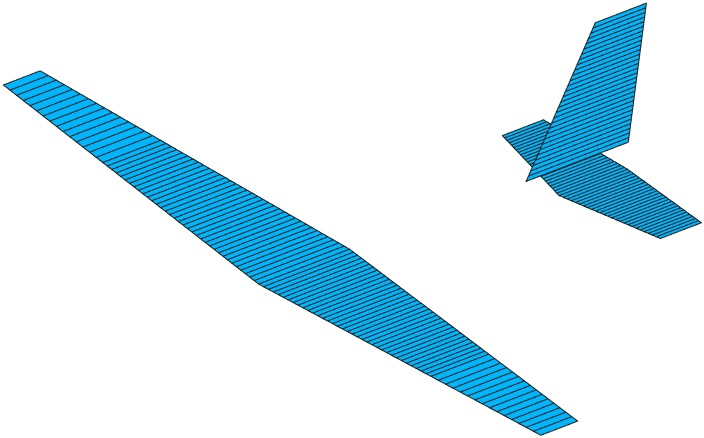
\includegraphics[width=0.7\textwidth]{Images-3-ProjetoDetalhado/vlm_paineis.jpeg} 
    \caption{Divisão dos painéis ao longo da envergadura no CEA-VLM.}
    \label{fig:vlm_paineis}
\end{figure}

Diferentemente de uma análise puramente potencial, que forneceria apenas a inclinação da curva de sustentação e o arrasto induzido linear, o CEA-VLM opera acoplando a solução 3D aos dados viscosos bidimensionais dos perfis aerodinâmicos. O algoritmo interpola as polares 2D dos perfis (coeficientes $C_L$, $C_D$ e $C_m$ em função de $\alpha$ e do número de Reynolds) para cada seção da asa e das empenagens. Este procedimento permite calcular os coeficientes globais tridimensionais de forma não linear, capturando efeitos viscosos como a perda de sustentação (estol) e o aumento do arrasto de perfil.

A geometria foi modelada reproduzindo as características descritas no Capítulo 4, utilizando os perfis NACA 43016 (raiz) e NACA 43009 (ponta) para a asa, e NACA 0012 para as empenagens.

Foram simuladas três condições operacionais distintas, considerando as deflexões de flap pertinentes a cada fase de voo.

O cálculo considerou a geometria completa da aeronave, variando-se o ângulo de ataque global ($\alpha$), mas mantendo a deflexão das superfícies de controle (profundor) nula em todos os pontos. Portanto, os valores representam a capacidade de geração de sustentação e o arrasto associado para a atitude da aeronave, sem o equilíbrio de momentos longitudinais.

O arrasto total apresentado nos gráficos é a soma do arrasto aerodinâmico calculado pelo CEA-VLM (induzido + viscoso da asa/empenagem) com o coeficiente de arrasto parasita da fuselagem e demais componentes ($C_{D_0}$) calculado analiticamente nas Seções 7.2 a 7.4.

As Figuras a seguir apresentam as polares obtidas para as três condições analisadas.

\begin{figure}[H]
    \centering
    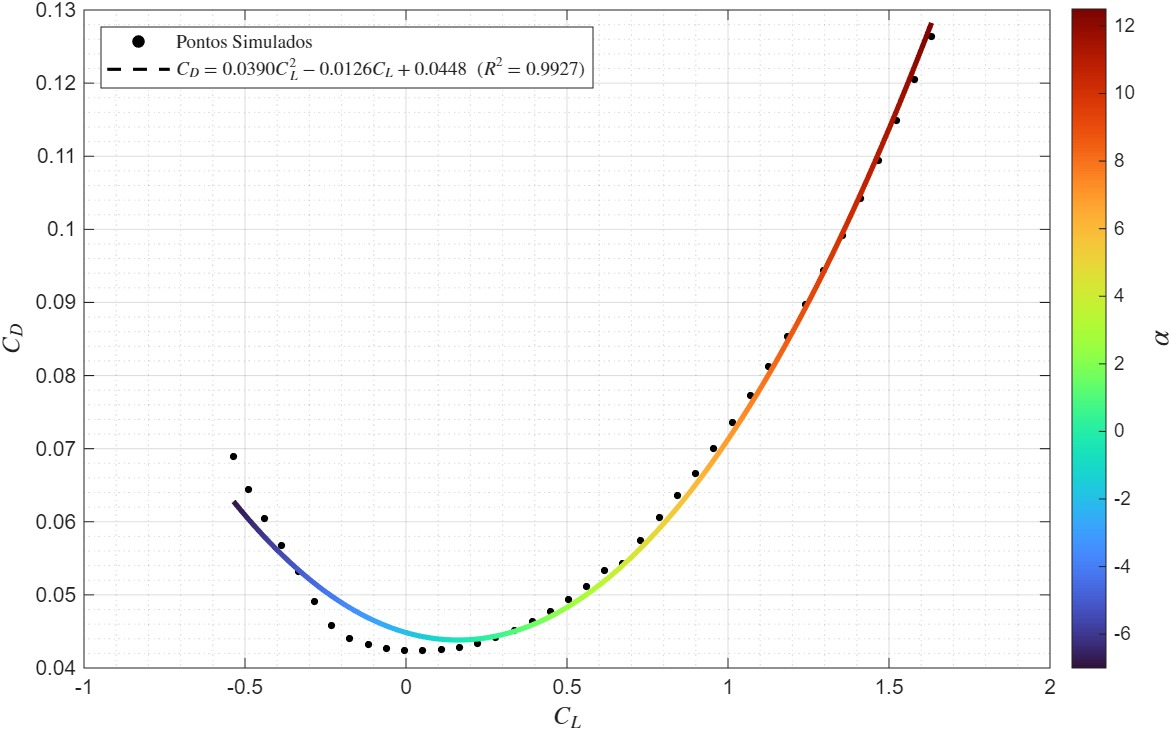
\includegraphics[width=0.7\textwidth]{Images-3-ProjetoDetalhado/polar_cruzeiro.jpeg} 
    \caption{Polar de Arrasto ($C_L \times C_D$) - Condição de Cruzeiro.}
    \label{fig:polar_cruzeiro}
\end{figure}

\begin{figure}[H]
    \centering
    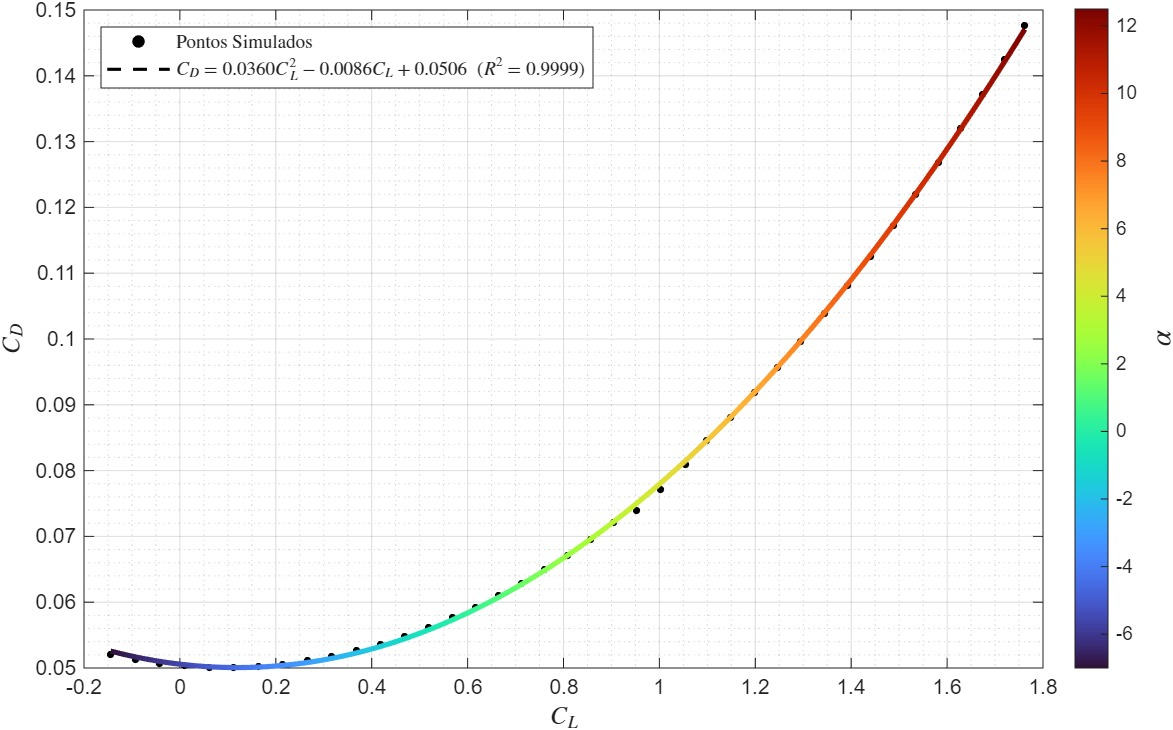
\includegraphics[width=0.7\textwidth]{Images-3-ProjetoDetalhado/polar_decolagem.jpeg}
    \caption{Polar de Arrasto ($C_L \times C_D$) - Condição de Decolagem.}
    \label{fig:polar_decolagem}
\end{figure}

\begin{figure}[H]
    \centering
    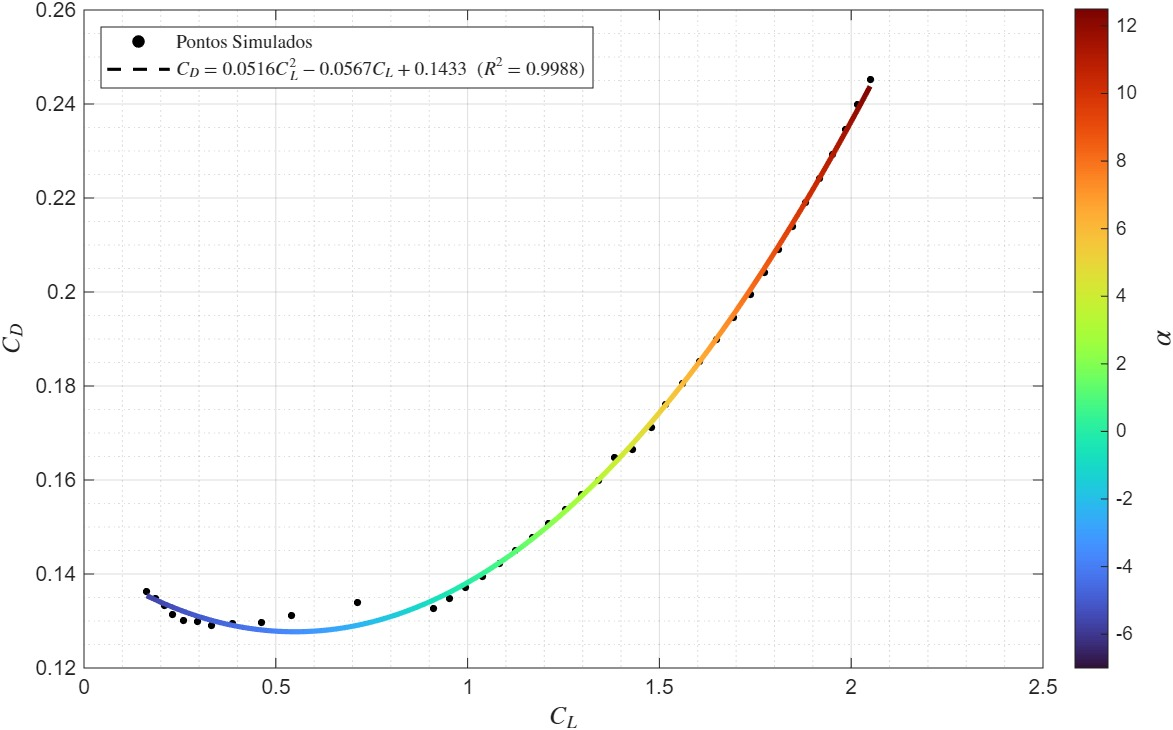
\includegraphics[width=0.7\textwidth]{Images-3-ProjetoDetalhado/polar_pouso.jpeg} 
    \caption{Polar de Arrasto ($C_L \times C_D$) - Condição de Pouso.}
    \label{fig:polar_pouso}
\end{figure}




\section{Cálculo das Potências}

\subsection{Curvas das Potências}

Para realizar os cálculos necessários para obter as curvas de potência \cite{medeiros2017}, foi preciso estimar os valores para 3 condições de voo diferentes, essas são: 

\begin{itemize}
    \item{Decolagem}
    \item{Cruzeiro}
    \item{Pouso}
\end{itemize}

Para traçar cada uma dessas curvas, é preciso obter os valores de potência requerida $P_{req}$ e de potência disponível $P_{disp}$, em relação à variação da velocidade da aeronave em uma determinada altura.

Para as condições de decolagem e cruzeiro, utiliza-se a potência requerida para voo sustentado. No pouso, entretanto, a aeronave encontra-se em trajetória descendente. Assim, a curva correspondente é interpretada como uma condição de planeio, na qual a perda de energia potencial gravitacional contribui para vencer o arrasto.

\subsubsection{Potência requerida:}

Primeiramente, para calcular a potência requerida, pode-se utilizar a seguinte equação que define ela.

\begin{equation}
P_{req} = D.V
\label{eq:preq}
\end{equation}

Na qual, D é a força de arrasto e V é a velocidade de interesse. Portanto, é necessário obter o arrasto e estimar uma velocidade para que o cálculo seja realizado. No entanto, D varia com a velocidade, ou seja, para cada um dos valores de velocidade, D irá variar.

Além disso, considerando que a aeronave estará em voo reto nivelado não acelerado, é possível demonstrar que:

\begin{equation}
C_L = \frac{L}{0.5 \cdot \rho \cdot V^2 \cdot S} = \frac{W}{0.5 \cdot \rho \cdot V^2 \cdot S}
\label{eq:cl}
\end{equation}

Ademais, o arrasto também pode ser definido pela equação utilizando o seu coeficiente:

\begin{equation}
C_D = \frac{D}{0.5 \cdot \rho \cdot V^2 \cdot S}
\label{eq:cd}
\end{equation}

Logo, ao substituir as equações \ref{eq:cl} e \ref{eq:cd} na equação \ref{eq:preq}, é possível chegar na seguinte relação que foi utilizada para traçar a curva de potência requerida pela velocidade:

\begin{equation}
P_{req} = \frac{W.V}{C_L/C_D}
\label{eq:preq2}
\end{equation}

Agora, para o procedimento de cálculo, é necessário que sejam calculados valores de $C_L$ para as diferentes velocidades, por meio da equação \ref{eq:cl}. Ao obter esses valores, pode-se utilizar os dados do gráfico da polar de arrasto para obter os valores de $C_D$ em relação à velocidade. Finalmente, com os valores obtidos, basta variar a V, para se obter o gráfico de interesse. Esse procedimento foi realizado para as 3 condições de voo e os seus cálculos são encontrados abaixo.

É importante notar que a densidade do ar ($\rho$) irá variar conforme a altitude considerada, mas obtendo-se ela os cálculos podem ser realizados.

\begin{itemize}
    \item{Decolagem:}
\end{itemize}

A altitude considerada para os cálculos foi ao nível do mar, ou seja, de acordo com a atmosfera ISA, $\rho = 1,225 \space kg/m^3$. Abaixo encontra-se a tabela com os valores obtidos.


\begin{table}[H]
\centering
\caption{Valores obtidos por meio dos cálculos - Decolagem.}
\begin{tabular}{c c c c}
\hline
Velocidade [m/s] & $C_L$ & $C_D$ & Potência Requerida [kW] \\
\hline
20 & 12{,}2560 & 5{,}3524 & 1943{,}4 \\
30 & 5{,}4469 & 1{,}0718 & 1313{,}4 \\
40 & 3{,}0639 & 0{,}3622 & 1052{,}1 \\
50 & 1{,}9609 & 0{,}1722 & 976{,}7 \\
60 & 1{,}3617 & 0{,}1056 & 1035{,}7 \\
70 & 1{,}0005 & 0{,}0780 & 1214{,}7 \\
80 & 0{,}7660 & 0{,}0651 & 1513{,}6 \\
90 & 0{,}6052 & 0{,}0586 & 1938{,}2 \\
100 & 0{,}4902 & 0{,}0550 & 2497{,}8 \\
110 & 0{,}4051 & 0{,}0530 & 3203{,}1 \\
\hline
\end{tabular}
\end{table}


\begin{itemize}
    \item{Cruzeiro:}
\end{itemize}

A altitude considerada para os cálculos foi à \text{20.000} pés, ou seja, de acordo com a atmosfera ISA, $\rho = \text{0,653} \space kg/m^3$. Abaixo encontra-se a tabela com os valores obtidos.

\begin{table}[H]
\centering
\caption{Valores obtidos por meio dos cálculos - Cruzeiro.}
\begin{tabular}{c c c c}
\hline
Velocidade [m/s] & $C_L$ & $C_D$ & Potência Requerida [kW] \\
\hline
50 & 3{,}6785 & 0{,}5262 & 1591{,}3 \\
60 & 2{,}5545 & 0{,}2671 & 1395{,}9 \\
70 & 1{,}8768 & 0{,}1585 & 1315{,}5 \\
80 & 1{,}4369 & 0{,}1072 & 1328{,}1 \\
90 & 1{,}1354 & 0{,}0808 & 1424{,}5 \\
100 & 0{,}9196 & 0{,}0662 & 1601{,}5 \\
110 & 0{,}7600 & 0{,}0578 & 1859{,}7 \\
120 & 0{,}6386 & 0{,}0527 & 2201{,}5 \\
130 & 0{,}5442 & 0{,}0495 & 2630{,}6 \\
140 & 0{,}4692 & 0{,}0475 & 3151{,}6 \\
150 & 0{,}4087 & 0{,}0462 & 3769{,}5 \\
160 & 0{,}3592 & 0{,}0453 & 4489{,}7 \\
\hline
\end{tabular}
\end{table}


\begin{itemize}
    \item{Pouso:}
\end{itemize}

Os cálculos foram realizados ao nível do mar em atmosfera padrão ($\rho = 1{,}225~\text{kg/m}^3$, ISA), considerando a aeronave no peso máximo de pouso ($\text{MLW} = 22\,350~\text{kgf}$). A Tabela~\ref{tab:pouso_p_req} reúne os resultados obtidos.

\begin{table}[H]
    \centering
    \caption{Valores obtidos por meio dos cálculos - Pouso (MLW).}
    \label{tab:pouso_p_req}
    \begin{tabular}{c c c c}
    \hline
        Velocidade [m/s] & $C_L$ & $C_D$ & Potência dissipada no planeio [kW] \\
    \hline
        20 & 12{,}0771 & 6{,}9769 & 2533{,}2 \\
        30 & 5{,}3676 & 1{,}3264 & 1625{,}4 \\
        40 & 3{,}0193 & 0{,}4429 & 1286{,}5 \\
        50 & 1{,}9323 & 0{,}2266 & 1285{,}4 \\
        60 & 1{,}3419 & 0{,}1602 & 1571{,}0 \\
        70 & 0{,}9859 & 0{,}1376 & 2141{,}7 \\
        80 & 0{,}7548 & 0{,}1299 & 3018{,}4 \\
        90 & 0{,}5964 & 0{,}1279 & 4232{,}2 \\
    \hline
    \end{tabular}
\end{table}

\subsubsection{Potência disponível:}

Primeiramente, é necessário determinar a potência de eixo (SHP) do motor para as três condições de voo analisadas. As potências foram estimadas com base na documentação técnica do motor PW120, pertencente à mesma família do PW127M, conforme a referência \cite{manual_pw120}. Para a decolagem, considerou-se a potência máxima de eixo disponível. Para o cruzeiro, adotou-se 79\% dessa potência e, para o pouso, 40\%, como hipóteses de operação utilizadas na análise de desempenho.


Portanto, os valores de potência no eixo foram estimados para cada condição de voo:

\begin{itemize}
    \item Decolagem:
    \[
        P_{\mathrm{SHP}} = 1{,}00\,P_{\max} = 4950~\mathrm{shp}
    \]

    \item Cruzeiro:
    \[
        P_{\mathrm{SHP}} = 0{,}79\,P_{\max} = 3910{,}5~\mathrm{shp}
    \]

    \item Pouso:
    \[
        P_{\mathrm{SHP}} = 0{,}40\,P_{\max} = 1980~\mathrm{shp}
    \]
\end{itemize}


Após obter o valor de SHP, é necessário considerar a eficiência da hélice para realizar o cálculo da $P_{disp}$, utilizando-se da seguinte relação:

\begin{equation}
    P_{\mathrm{disp}} = \eta_{\mathrm{prop}}\,P_{\mathrm{SHP}}
    \label{eq:pdisp}
\end{equation}

Para isso é necessário utilizar o gráfico da eficiência da hélice em função da razão de avanço da mesma ($J$). Entretanto as curvas de eficiência para a hélice \textit{Hamilton Standard 568F} estão sob sigilo empresarial. Dessa forma, adotaram-se as curvas de eficiência da hélice \textit{Clark Y}. Nesse sentido, a equação da razão de avanço é apresentada a seguir:



\begin{equation}
J = \frac{V}{n \cdot D}
\label{eq:avanco}
\end{equation}


Foi considerado o valor de 1200 rotações por minuto para as três condições de voo, adotando-se um ângulo de pá de 15° para decolagem e pouso e de 30° para cruzeiro. Como a aeronave possui hélices de passo variável, para razões de avanço que ultrapassam os limites das curvas correspondentes aos ângulos de pá definidos, adota-se a maior eficiência disponível. A seguir, apresentam-se as tabelas com os valores da razão de avanço em função da velocidade para cada condição de voo.

\begin{itemize}
    \item{Decolagem:}
\end{itemize}


\begin{table}[H]
\centering
\caption{Razão de avanço $J$ e eficiência $\eta_{\mathrm{prop}}$ em função da velocidade de voo - Decolagem.}
\begin{tabular}{ccc}
\hline
Velocidade [m/s] & $J$ & $\eta_{\mathrm{prop}}$ \\
\hline
20 & 0{,}2545 & 0{,}50 \\
30 & 0{,}3817 & 0{,}65 \\
40 & 0{,}5089 & 0{,}78 \\
50 & 0{,}6361 & 0{,}82 \\
60 & 0{,}7634 & 0{,}84 \\
70 & 0{,}8906 & 0{,}82 \\
80 & 1{,}0178 & 0{,}78 \\
90 & 1{,}1450 & 0{,}73 \\
100 & 1{,}2723 & 0{,}67 \\
110 & 1{,}3995 & 0{,}64 \\
\hline
\end{tabular}
\end{table}


\begin{itemize}
    \item{Cruzeiro:}
\end{itemize}

\begin{table}[H]
\centering
\caption{Razão de avanço $J$ e eficiência $\eta_{\mathrm{prop}}$ em função da velocidade de voo - Cruzeiro.}
\begin{tabular}{ccc}
\hline
Velocidade [m/s] & $J$ & $\eta_{\mathrm{prop}}$ \\
\hline
50 & 0{,}6361 & 0{,}50 \\
60 & 0{,}7634 & 0{,}70 \\
70 & 0{,}8906 & 0{,}78 \\
80 & 1{,}0178 & 0{,}82 \\
90 & 1{,}1450 & 0{,}84 \\
100 & 1{,}2723 & 0{,}85 \\
110 & 1{,}3995 & 0{,}84 \\
120 & 1{,}5267 & 0{,}82 \\
130 & 1{,}6539 & 0{,}81 \\
140 & 1{,}7812 & 0{,}79 \\
150 & 1{,}9084 & 0{,}77 \\
160 & 2{,}0356 & 0{,}75 \\
\hline
\end{tabular}
\end{table}

\clearpage
\begin{itemize}
    \item{Pouso:}
\end{itemize}

\begin{table}[H]
\centering
\caption{Razão de avanço $J$ e eficiência $\eta_{\mathrm{prop}}$ em função da velocidade de voo - Pouso.}
\begin{tabular}{ccc}
\hline
Velocidade [m/s] & $J$ & $\eta_{\mathrm{prop}}$ \\
\hline
20 & 0{,}2545 & 0{,}50 \\
30 & 0{,}3817 & 0{,}65 \\
40 & 0{,}5089 & 0{,}78 \\
50 & 0{,}6361 & 0{,}82 \\
60 & 0{,}7634 & 0{,}84 \\
70 & 0{,}8906 & 0{,}82 \\
80 & 1{,}0178 & 0{,}81 \\
90 & 1{,}1450 & 0{,}80 \\
\hline
\end{tabular}
\end{table}


Com os valores da eficiência e do \textit{Shaft Horsepower}, é possível estimar a potência disponível em função da velocidade para cada uma das condições.

\begin{itemize}
    \item{Decolagem:}
\end{itemize}

\begin{table}[H]
\centering
\caption{Velocidade e potência disponível - Decolagem.}
\begin{tabular}{cc}
\hline
Velocidade [m/s] & Potência disponível [kW] \\
\hline
20 & 1845{,}6 \\
30 & 2399{,}3 \\
40 & 2879{,}2 \\
50 & 3026{,}8 \\
60 & 3100{,}6 \\
70 & 3026{,}8 \\
80 & 2879{,}2 \\
90 & 2694{,}6 \\
100 & 2473{,}1 \\
110 & 2362{,}4 \\
\hline
\end{tabular}
\end{table}

\clearpage

\begin{itemize}
    \item{Cruzeiro:}
\end{itemize}

\begin{table}[H]
\centering
\caption{Velocidade e potência disponível - Cruzeiro.}
\begin{tabular}{cc}
\hline
Velocidade [m/s] & Potência disponível [kW] \\
\hline
50 & 1458{,}0 \\
60 & 2041{,}2 \\
70 & 2274{,}5 \\
80 & 2391{,}2 \\
90 & 2449{,}5 \\
100 & 2478{,}7 \\
110 & 2449{,}5 \\
120 & 2391{,}2 \\
130 & 2362{,}0 \\
140 & 2303{,}7 \\
150 & 2245{,}4 \\
160 & 2187{,}0 \\
\hline
\end{tabular}
\end{table}

\begin{itemize}
    \item{Pouso:}
\end{itemize}

\begin{table}[H]
\centering
\caption{Velocidade e potência disponível - Pouso.}
\begin{tabular}{cc}
\hline
Velocidade [m/s] & Potência disponível [kW] \\
\hline
20 & 738{,}24 \\
30 & 959{,}72 \\
40 & 1151{,}7 \\
50 & 1210{,}7 \\
60 & 1240{,}2 \\
70 & 1210{,}7 \\
80 & 1196{,}0 \\
90 & 1181{,}2 \\
\hline
\end{tabular}
\end{table}

\subsubsection{Gráficos obtidos}

Finalmente, com todos os valores obtidos pelos cálculos, foi possível traçar os gráficos necessários. Todos os 3 podem ser encontrados abaixo.

\clearpage

\begin{itemize}
    \item{Decolagem:}
\end{itemize}

\begin{figure}[H]
    \centering
    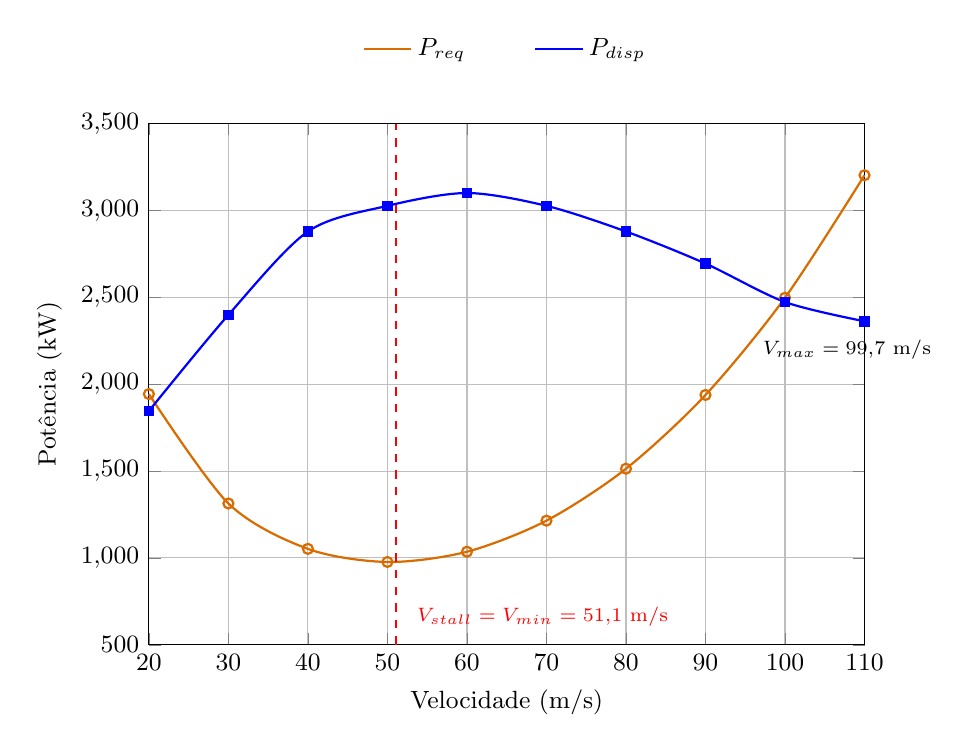
\begin{tikzpicture}
    \begin{axis}[
        width=0.88\textwidth,
        height=8.2cm,
        xlabel={Velocidade (m/s)},
        ylabel={Potência (kW)},
        xmin=20, xmax=110,
        ymin=500, ymax=3500,
        grid=major,
        tick label style={font=\small},
        label style={font=\small},
        legend columns=2,
        legend style={
            at={(0.5,1.10)},
            anchor=south,
            font=\small,
            draw=none,
            fill=none,
            /tikz/every even column/.append style={column sep=0.8cm}
        },
        clip=false,
        every axis plot/.append style={thick}
    ]

    % Potência requerida (Tabela 7.10, MTOW)
    \addplot[color=orange!85!black, smooth, mark=none] coordinates {
        (20,1943.4) (30,1313.4) (40,1052.1) (50,976.7) (60,1035.7)
        (70,1214.7) (80,1513.6) (90,1938.2) (100,2497.8) (110,3203.1)
    };
    \addlegendentry{$P_{req}$}
    \addplot[only marks, color=orange!85!black, mark=o, mark options={scale=0.9}, forget plot] coordinates {
        (20,1943.4) (30,1313.4) (40,1052.1) (50,976.7) (60,1035.7)
        (70,1214.7) (80,1513.6) (90,1938.2) (100,2497.8) (110,3203.1)
    };

    % Potência disponível (Tabela 7.16)
    \addplot[color=blue, smooth, mark=none] coordinates {
        (20,1845.6) (30,2399.3) (40,2879.2) (50,3026.8) (60,3100.6)
        (70,3026.8) (80,2879.2) (90,2694.6) (100,2473.1) (110,2362.4)
    };
    \addlegendentry{$P_{disp}$}
    \addplot[only marks, color=blue, mark=square*, mark options={scale=0.75}, forget plot] coordinates {
        (20,1845.6) (30,2399.3) (40,2879.2) (50,3026.8) (60,3100.6)
        (70,3026.8) (80,2879.2) (90,2694.6) (100,2473.1) (110,2362.4)
    };

    % Velocidade de estol com flap 10° (Seção 7.6)
    \addplot[red, dashed, thick] coordinates {(51.1,500) (51.1,3500)};

    % Anotações
    \node[red, anchor=west, font=\scriptsize] at (axis cs:52.5,660)
        {$V_{stall}=V_{min}=51{,}1\ \mathrm{m/s}$};
    \node[anchor=west, font=\scriptsize] at (axis cs:96,2200)
        {$V_{max}=99{,}7\ \mathrm{m/s}$};

    \end{axis}
    \end{tikzpicture}
    \caption{Curvas de potência na decolagem com $10^\circ$ de flap (nível do mar, 100\% SHP, MTOW).}
    \label{fig:potencia_decolagem_suave}
\end{figure}

Para uma análise com mais detalhes, sugere-se também a análise das curvas sem deflexão dos flaps, haja vista que para velocidades altas algumas aeronaves podem não acionar os flaps na decolagem.


\clearpage


\begin{itemize}
    \item{Cruzeiro:}
\end{itemize}

\begin{figure}[H]
    \centering
    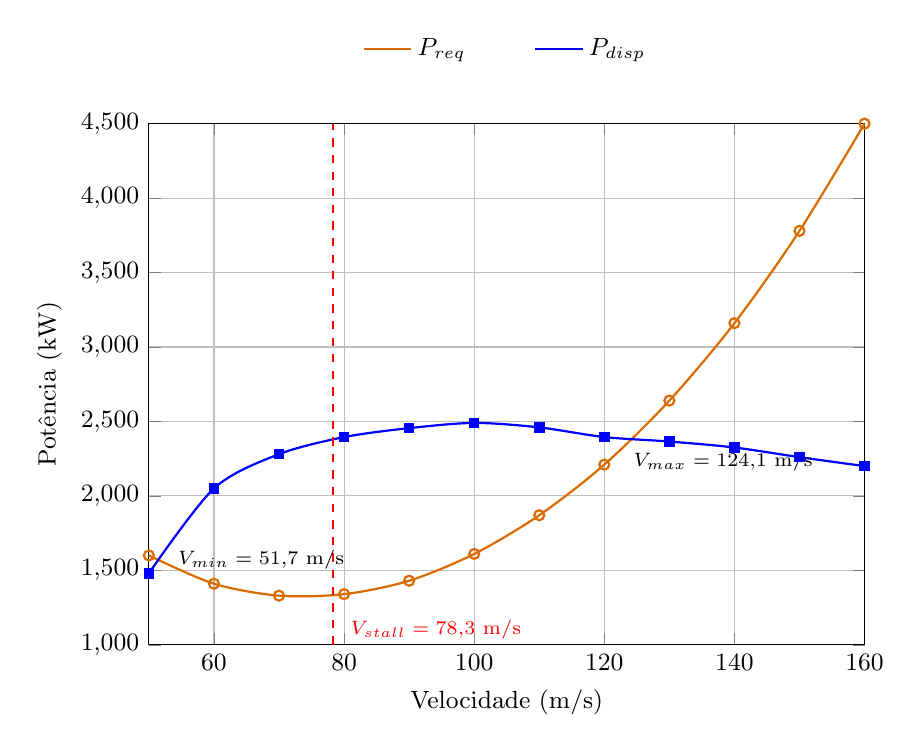
\begin{tikzpicture}
    \begin{axis}[
        width=0.88\textwidth,
        height=8.2cm,
        xlabel={Velocidade (m/s)},
        ylabel={Potência (kW)},
        xmin=50, xmax=160,
        ymin=1000, ymax=4500,
        grid=major,
        tick label style={font=\small},
        label style={font=\small},
        legend columns=2,
        legend style={
            at={(0.5,1.10)},
            anchor=south,
            font=\small,
            draw=none,
            fill=none,
            /tikz/every even column/.append style={column sep=0.8cm}
        },
        clip=false,
        every axis plot/.append style={thick}
    ]

    % -------------------------
    % Potência requerida
    % -------------------------
    \addplot[
        color=orange!85!black,
        smooth,
        mark=none
    ] coordinates {
        (50,1600)
        (60,1410)
        (70,1330)
        (80,1340)
        (90,1430)
        (100,1610)
        (110,1870)
        (120,2210)
        (130,2640)
        (140,3160)
        (150,3780)
        (160,4500)
    };
    \addlegendentry{$P_{req}$}

    \addplot[
        only marks,
        color=orange!85!black,
        mark=o,
        mark options={scale=0.9},
        forget plot
    ] coordinates {
        (50,1600)
        (60,1410)
        (70,1330)
        (80,1340)
        (90,1430)
        (100,1610)
        (110,1870)
        (120,2210)
        (130,2640)
        (140,3160)
        (150,3780)
        (160,4500)
    };

    % -------------------------
    % Potência disponível
    % -------------------------
    \addplot[
        color=blue,
        smooth,
        mark=none
    ] coordinates {
        (50,1480)
        (60,2050)
        (70,2280)
        (80,2395)
        (90,2455)
        (100,2490)
        (110,2460)
        (120,2395)
        (130,2365)
        (140,2325)
        (150,2260)
        (160,2200)
    };
    \addlegendentry{$P_{disp}$}

    \addplot[
        only marks,
        color=blue,
        mark=square*,
        mark options={scale=0.75},
        forget plot
    ] coordinates {
        (50,1480)
        (60,2050)
        (70,2280)
        (80,2395)
        (90,2455)
        (100,2490)
        (110,2460)
        (120,2395)
        (130,2365)
        (140,2325)
        (150,2260)
        (160,2200)
    };

    % -------------------------
    % Linha da velocidade de estol
    % -------------------------
    \addplot[
        red,
        dashed,
        thick
    ] coordinates {(78.3,1000) (78.3,4500)};

    % -------------------------
    % Anotações
    % -------------------------
    \node[anchor=west, font=\scriptsize] at (axis cs:53,1570)
        {$V_{min}=51{,}7\ \mathrm{m/s}$};

    \node[red, anchor=west, font=\scriptsize] at (axis cs:79.5,1100)
        {$V_{stall}=78{,}3\ \mathrm{m/s}$};

    \node[anchor=west, font=\scriptsize] at (axis cs:123,2230)
        {$V_{max}=124{,}1\ \mathrm{m/s}$};

    \end{axis}
    \end{tikzpicture}
    \caption{Curvas de potência no cruzeiro (20.000 ft, 79\% SHP).}
    \label{fig:potencia_cruzeiro_suave}
\end{figure}


\begin{itemize}
    \item{Pouso:}
\end{itemize}

\begin{figure}[H]
    \centering
    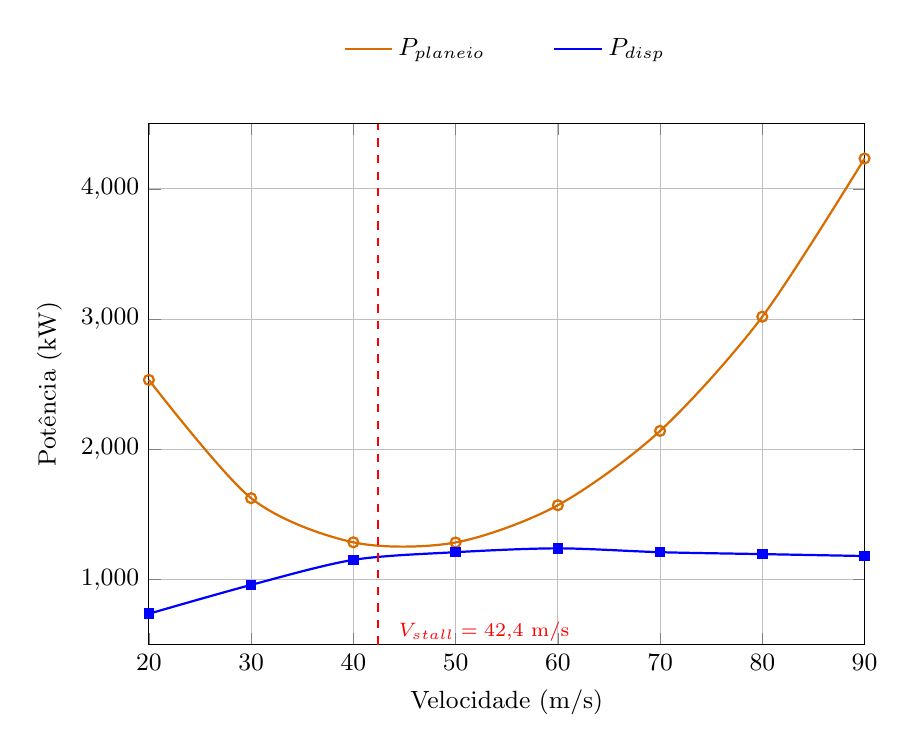
\begin{tikzpicture}
    \begin{axis}[
        width=0.88\textwidth,
        height=8.2cm,
        xlabel={Velocidade (m/s)},
        ylabel={Potência (kW)},
        xmin=20, xmax=90,
        ymin=500, ymax=4500,
        grid=major,
        tick label style={font=\small},
        label style={font=\small},
        legend columns=2,
        legend style={
            at={(0.5,1.10)},
            anchor=south,
            font=\small,
            draw=none,
            fill=none,
            /tikz/every even column/.append style={column sep=0.8cm}
        },
        clip=false,
        every axis plot/.append style={thick}
    ]

    % Condição de planeio (Tabela 7.12, MLW)
    \addplot[color=orange!85!black, smooth, mark=none] coordinates {
        (20,2533.2) (30,1625.4) (40,1286.5) (50,1285.4)
        (60,1571.0) (70,2141.7) (80,3018.4) (90,4232.2)
    };
    \addlegendentry{$P_{planeio}$}
    \addplot[only marks, color=orange!85!black, mark=o, mark options={scale=0.9}, forget plot] coordinates {
        (20,2533.2) (30,1625.4) (40,1286.5) (50,1285.4)
        (60,1571.0) (70,2141.7) (80,3018.4) (90,4232.2)
    };

    % Potência disponível (Tabela 7.18)
    \addplot[color=blue, smooth, mark=none] coordinates {
        (20,738.2) (30,959.7) (40,1151.7) (50,1210.7)
        (60,1240.2) (70,1210.7) (80,1196.0) (90,1181.2)
    };
    \addlegendentry{$P_{disp}$}
    \addplot[only marks, color=blue, mark=square*, mark options={scale=0.75}, forget plot] coordinates {
        (20,738.2) (30,959.7) (40,1151.7) (50,1210.7)
        (60,1240.2) (70,1210.7) (80,1196.0) (90,1181.2)
    };

    % Velocidade de estol com flap 40°, MLW (Seção 7.6)
    \addplot[red, dashed, thick] coordinates {(42.4,500) (42.4,4500)};

    % Anotações
    \node[red, anchor=west, font=\scriptsize] at (axis cs:43.5,600)
        {$V_{stall}=42{,}4\ \mathrm{m/s}$};

    \end{axis}
    \end{tikzpicture}
    \caption{Condição de planeio e potência disponível no pouso com $40^\circ$ de flap (nível do mar, 40\% SHP, MLW).}
    \label{fig:potencia_pouso_suave}
\end{figure}

Assim como comentado nas curvas de potência para decolagem, no pouso sugere-se, em análises posteriores, a verificação de pouso sem deflexão dps flaps e/ou com angulações menores.

\section{Velocidades Máximas, Mínimas e Estol}

A velocidade máxima e mínima de voo em cada condição podem ser determinadas por meio dos gráficos de velocidade x potência. Quando a curva de potência requerida cruza a curva de potência disponível, sabe-se que são nesses pontos que se encontram as velocidades mínimas e máximas de operação, entretanto quando a velocidade mínima através da interseção das curvas é inferior a de estol, a velocidade de estol é a mínima de voo, abaixo encontram-se os valores obtidos para as 3 condições.

\begin{itemize}
    \item{Decolagem:}
\end{itemize}

\begin{equation}
    V_{min,decolagem} = 51{,}1 \text{ m/s} = 99{,}3 \text{ kt}
\end{equation}

\begin{equation}
    V_{max,decolagem} = 99{,}7 \text{ m/s} = 193{,}8 \text{ kt}
\end{equation}


\begin{itemize}
    \item{Cruzeiro:}
\end{itemize}


\begin{equation}
    V_{min,cruzeiro} = 78{,}3 \text{ m/s} = 152{,}2 \text{ kt}
\end{equation}

\begin{equation}
    V_{max,cruzeiro} = 124{,}1 \text{ m/s} = 241{,}3 \text{ kt}
\end{equation}

\begin{itemize}
    \item Pouso:
\end{itemize}

Na condição de pouso, não se utiliza a interseção entre potência requerida e potência disponível para determinar os limites de velocidade, pois a aeronave encontra-se em trajetória descendente. A aproximação é tratada como uma condição de planeio, na qual a perda de energia potencial contribui para vencer o arrasto. Dessa forma, a velocidade de aproximação é definida a partir da velocidade de estol e dos fatores de segurança adotados para o pouso.

\begin{itemize}
    \item \textbf{Velocidade de Estol:}
\end{itemize}

As velocidades de estol para cada condição operacional são determinadas pela Equação~5.10, empregando o peso correspondente à fase de voo (Tabela~\ref{tab:cg_entradas}) e os coeficientes de sustentação máximos de cada configuração aerodinâmica ($C_{L\max} = 1{,}50$ em configuração limpa, $1{,}88$ com flap a $10^\circ$ e $2{,}69$ com flap a $40^\circ$, valores consistentes com o diagrama $V\text{--}n$ da Seção~9.2). Cabe ressaltar que os coeficientes de $1{,}17$ e $1{,}59$ reportados na Tabela~5.2 correspondem às condições operacionais de decolagem ($1{,}13\,V_S$) e pouso ($1{,}30\,V_S$), e não aos limites de estol.

\begin{itemize}
    \item \textbf{Pouso (nível do mar, flap $40^\circ$, MLW):}
    \begin{equation}
        V_{S,L} = \sqrt{\frac{2 \cdot 22\,350 \cdot 9{,}81}{1{,}225 \cdot 74{,}1 \cdot 2{,}69}} = 42{,}4~\text{m/s} \approx 82{,}4~\text{kt}
    \end{equation}

    \item \textbf{Decolagem (nível do mar, flap $10^\circ$, MTOW):}
    \begin{equation}
        V_{S,TO} = \sqrt{\frac{2 \cdot 22\,680 \cdot 9{,}81}{1{,}225 \cdot 74{,}1 \cdot 1{,}88}} = 51{,}1~\text{m/s} \approx 99{,}3~\text{kt}
    \end{equation}

    \item \textbf{Configuração limpa (MTOW):} $V_S = 57{,}2~\text{m/s}$ ($111~\text{kt}$) ao nível do mar, conforme a Tabela~5.2, atingindo $V_S = 78{,}3~\text{m/s}$ ($152{,}2~\text{kt}$ TAS) a $20\,000~\text{ft}$ ($\rho = 0{,}653~\text{kg/m}^3$).
\end{itemize}

A partir desses limites, obtêm-se a velocidade operacional de aproximação ($1{,}30\,V_{S,L} = 55{,}1~\text{m/s}$ ou $107{,}1~\text{kt}$) e a velocidade de decolagem de $125~\text{kt}$ apresentada na Tabela~5.2.


\section{Distância de Decolagem}

A avaliação do desempenho de decolagem do turboélice regional fundamenta-se nos requisitos de certificação da categoria transporte estabelecidos pelo 14 CFR Part~25 e pelo RBAC~25~\cite{far25}. Os cálculos consideram operação ao nível do mar em atmosfera padrão (ISA), com os motores em potência máxima de decolagem, a aeronave em seu peso máximo de decolagem (MTOW) e coeficiente de atrito de rolamento $\mu = 0{,}02$, representativo de pista seca de concreto.

Pelo \S25.113, a distância de decolagem corresponde ao maior valor entre o percurso até $35~\text{ft}$ com falha do motor crítico (OEI) e $115\%$ do percurso até a mesma altura com todos os motores operantes (AEO). Complementarmente, o \S25.109 define a distância de aceleração-parada para o caso de decolagem abortada após a falha. Nas subseções seguintes, determina-se inicialmente o desempenho com todos os motores operando (Seções~7.7.1 a 7.7.3) e, na sequência, analisa-se a condição monomotora por meio do comprimento de pista balanceado (BFL), na Seção~7.7.4.

Os critérios normativos aplicáveis estão esquematizados na Figura~\ref{fig:fases_decolagem}.

\begin{figure}[H]
\centering
\resizebox{\textwidth}{!}{%
\begin{tikzpicture}[x=1cm,y=1cm,font=\small,
  dim/.style={{Latex[length=2mm]}-{Latex[length=2mm]},thin},
  vline/.style={densely dotted,gray}]
  % pista
  \fill[gray!15] (0,-0.12) rectangle (14.6,0);
  \draw[thick] (0,0) -- (14.6,0);
  % altura de 35 ft
  \draw[gray,dashed] (0,1.6) -- (14.6,1.6);
  \node[gray,anchor=west] at (12.25,1.85) {35 ft (10,7 m)};
  % todos os motores operando (AEO)
  \draw[very thick,blue!70!black] (0,0) -- (5.4,0)
     .. controls (6.6,0.05) and (7.4,0.9) .. (8.4,1.6) -- (9.0,2.0);
  % motor crítico inoperante (OEI)
  \draw[very thick,red!75!black,dashed] (3.2,0.03) -- (7.2,0.03)
     .. controls (8.6,0.08) and (9.9,0.95) .. (11.0,1.6) -- (11.8,2.0);
  % aceleração-parada
  \draw[very thick,green!45!black,dash dot] (4.0,-0.35) -- (11.0,-0.35);
  \draw[green!45!black] (4.0,-0.2) -- (4.0,-0.5);
  \fill[green!45!black] (11.0,-0.35) circle (1.8pt);
  \node[green!45!black,anchor=north,font=\footnotesize] at (7.5,-0.38) {Frenagem após $V_1$ (parada)};
  % marcas de velocidade
  \draw[vline] (3.2,0) -- (3.2,2.6) node[above] {$V_{EF}$};
  \draw[vline] (4.0,0) -- (4.0,2.6) node[above] {$V_1$};
  \draw[vline] (5.4,0) -- (5.4,2.6) node[above] {$V_{LOF}$};
  \draw[vline] (11.0,0) -- (11.0,2.6) node[above] {$V_2$};
  \node[blue!70!black,anchor=east] at (7.3,1.2) {AEO};
  \node[red!75!black,anchor=west] at (10.0,0.55) {OEI};
  % cotas
  \draw[dim] (0,-1.1) -- (8.4,-1.1) node[midway,fill=white,inner sep=1pt] {$d_{AEO}$ (até 35 ft)};
  \draw[dim] (0,-1.65) -- (9.66,-1.65) node[midway,fill=white,inner sep=1pt] {$1{,}15\,d_{AEO}$};
  \draw[dim] (0,-2.2) -- (11.0,-2.2) node[midway,fill=white,inner sep=1pt] {$d_{OEI}$: Falha do motor crítico em $V_{EF}$ (§25.113(a)(1))};
  \draw[dim] (0,-2.75) -- (11.0,-2.75) node[midway,fill=white,inner sep=1pt] {Distância de aceleração--parada (§25.109)};
  % linhas de chamada das cotas
  \draw[thin,gray] (0,-0.6)    -- (0,-2.9);
  \draw[thin,gray] (8.4,-0.8)  -- (8.4,-1.2);
  \draw[thin,gray] (9.66,-0.8) -- (9.66,-1.75);
  \draw[thin,gray] (11.0,-0.5) -- (11.0,-2.9);
  % legenda lateral
  \node[anchor=west,align=left,font=\footnotesize] at (11.4,-1.9)
     {Distância de decolagem\\$=\max\{d_{OEI};\,1{,}15\,d_{AEO}\}$\\[2pt]
      BFL: $d_{OEI} = $ Dist. de\\aceleração--parada};
\end{tikzpicture}%
}
\caption{Distâncias de decolagem da categoria transporte (alturas fora de escala). Elaborado pelos autores com base no 14 CFR Part 25, §25.109 e §25.113 \cite{far25}.}
\label{fig:fases_decolagem}
\end{figure}

\subsection{Corrida no Solo}
O deslocamento inicial da aeronave sobre a pista, do repouso até $V_{lof}$ na Figura~\ref{fig:fases_decolagem}, define a corrida de decolagem. A velocidade de decolagem ($V_{lof}$) é estimada pela seguinte proporção empírica em relação ao limite de estol:
\begin{equation}
    V_{lof} = 1,13 \cdot V_{s}
\end{equation}
\begin{equation}
    V_{lof} = 125 \text{ kt}= 64,3 \text{ m/s}
\end{equation}

A modelagem dinâmica dessa fase baseia-se na aplicação da Segunda Lei de Newton, equacionando as forças nos eixos horizontal e vertical durante a aceleração da aeronave:
\begin{equation}
    T - D - \mu(W - L) = \frac{W}{g} \cdot \frac{dV}{dt}
\end{equation}
\begin{equation}
    N = W - L
\end{equation}

Sabendo que a aceleração instantânea pode ser reescrita em função do espaço percorrido:
\begin{equation}
    a = \frac{dV}{dt} = \frac{1}{2}\frac{dV^{2}}{dS}
\end{equation}

Isolando o diferencial de espaço e integrando o movimento do repouso até o \textit{lift-off}, encontra-se a distância total de corrida no solo ($S$), conforme a Equação \ref{eq:dist_corrida}:
\begin{equation}
    S = \int_{0}^{V_{LOF}} \frac{W}{2g(T - D)} dV^{2}
    \label{eq:dist_corrida}
\end{equation}

Implementando um algoritmo de integração numérica iterativa, o espaço de corrida calculado foi de:
\begin{equation}
    S = 907,46 \text{ m}
\end{equation}

\subsection{Subida de Decolagem}
Para estimar as distâncias na subida de decolagem, o cálculo foi dividido em duas etapas. A primeira ($S_{1}$) descreve a trajetória curva de transição, modelada como um arco de círculo. O segmento subsequente ($S_{2}$) retrata o trecho de ascensão em trajetória retilínea até o momento em que o trem de pouso cruza a altura estipulada do obstáculo virtual. A geometria dessa transição está demonstrada na Figura \ref{fig:subida_decolagem}.

\begin{figure}[H]
    \centering
    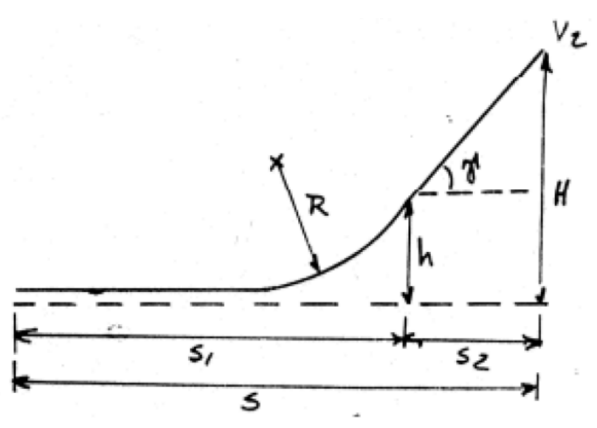
\includegraphics[width=0.6\textwidth]{Images-3-ProjetoDetalhado/subida_decolagem.png} 
    \caption{Subida de decolagem inicial.}
    \label{fig:subida_decolagem}
\end{figure}

Conforme sugerido por Gudmundsson \cite{Gudmundsson}, a velocidade característica ao longo da manobra de arredondamento obedece à relação apresentada na Equação \ref{eq:v_inf}:
\begin{equation}
    V_{\infty} = 1,2 \cdot V_{S}
    \label{eq:v_inf}
\end{equation}
\begin{equation}
    V_{\infty} = 67,1 \text{ m/s}
\end{equation}

O equilíbrio dinâmico radial durante o arco de trajetória é então expresso por:
\begin{equation}
    F_{R} = m \cdot a = m\frac{V_{\infty}^{2}}{R} = L - W \cos \theta
\end{equation}

Como o ângulo da trajetória em relação à horizontal ($\theta$) é pequeno, assume-se que $\cos \theta \approx 1$. Com esta simplificação geométrica, o raio da curva de transição ($R$) é isolado na Equação \ref{eq:raio_subida}:
\begin{equation}
    R = \frac{V_{\infty}^{2}}{g(n - 1)}
    \label{eq:raio_subida}
\end{equation}

Considerando a premissa aerodinâmica de que o $C_{L}$ da manobra atinge cerca de $0,9 \cdot C_{L_{max}}$, considerou-se que o fator de carga para a curva de decolagem é de:
\begin{equation}
    n = \frac{L}{W} = 1,3
\end{equation}

Aplicando este coeficiente na Equação \ref{eq:raio_subida}, obtém-se o raio da trajetória de subida:
\begin{equation}
    R = 1529,9 \text{ m}
\end{equation}

A projeção horizontal da distância percorrida durante esta manobra em arco ($S_{1}$) é obtida geometricamente pela Equação \ref{eq:s1}:
\begin{equation}
    S_{1} = R \cdot \sin \gamma
    \label{eq:s1}
\end{equation}
\begin{equation}
    S_{1} = 122,71 \text{ m}
\end{equation}

Onde $\gamma$ representa o ângulo máximo de subida, estimado pelo balanço de forças longitudinais:
\begin{equation}
    \gamma = \sin^{-1}\left(\frac{T - D}{W}\right) \approx 4,6 ^\circ
\end{equation}

O ganho de altitude correspondente a este segmento ($h$) pode ser aproximado pela correlação geométrica expressa na Equação \ref{eq:altura_transicao}:
\begin{equation}
    h = \frac{S_{1}^{2}}{2 \cdot R}
    \label{eq:altura_transicao}
\end{equation}
\begin{equation}
    h = 4,92 \text{ m}
\end{equation}

Em seguida, o segmento $S_{2}$ é computado admitindo-se uma taxa de subida constante até passar de um obstáculo padrão ($H$) definido pelo 14 CFR Part 25. Fixou-se, então, $H = 35 \text{ ft (10,66 m)}$. O espaço horizontal deste trecho retilíneo torna-se, portanto:
\begin{equation}
    S_{2} = \frac{H - h}{\tan \gamma}
\end{equation}
\begin{equation}
    S_{2} = 71,42 \text{ m}
\end{equation}

\subsection{Distância Total de Decolagem}
Por fim, o comprimento exigido de pista para que a aeronave complete toda a operação de decolagem em segurança é a somatória das etapas elucidadas:
\begin{equation}
    S_{decolagem} = S + S_{1} + S_{2}
\end{equation}
\begin{equation}
    S_{decolagem} = 1101,59\text{ m}
\end{equation}

Esse valor corresponde à decolagem com todos os motores operando. A verificação do requisito de 4 200 ft (1 280 m), no entanto, é feita pela condição monomotora, apresentada na Seção 7.7.4.

\subsection{Comprimento de Pista Balanceado (BFL)}
\label{sec:bfl}
O comprimento de pista balanceado (\emph{Balanced Field Length} -- BFL) corresponde ao comprimento para o qual a interrupção da decolagem e sua continuação após a falha do motor crítico exigem a mesma distância. Sua estimativa foi realizada pelo método semiempírico de Raymer \cite{raymer2018}, considerando atmosfera ISA ao nível do mar, pista seca e horizontal, ausência de vento e peso máximo de decolagem de $22\,680~\mathrm{kgf}$. Foram utilizadas a geometria e as características propulsivas apresentadas anteriormente, adotando-se o valor de $C_{L_{\max,TO}}$ retirado da polar de decolagem.

A velocidade de subida inicial e o coeficiente de sustentação correspondente foram determinados por:
\begin{equation}
    V_2 = 1{,}2
    \sqrt{\frac{2W}{\rho S C_{L_{\max,TO}}}},
    \qquad
    C_{L,\mathrm{sub}} =
    \frac{C_{L_{\max,TO}}}{1{,}2^2}.
\end{equation}

Para a subida monomotor, consideraram-se o trem de pouso recolhido e a hélice do motor inoperante embandeirada. O coeficiente de arrasto foi obtido corrigindo a polar de decolagem:
\begin{equation}
    C_{D,\mathrm{OEI}} =
    C_{D,\mathrm{TO}}(C_{L,\mathrm{sub}})
    - \Delta C_{D,\mathrm{LG}}
    + \Delta C_{D,\text{hélice}}.
\end{equation}

O arrasto e a tração do motor remanescente foram calculados por:
\begin{equation}
    D_{\mathrm{OEI}} =
    \frac{1}{2}\rho V_2^2 S C_{D,\mathrm{OEI}},
    \qquad
    T_{\mathrm{OEI}} =
    \frac{\eta_p P_{\mathrm{eixo},1}}{V_2},
\end{equation}
com a eficiência propulsiva interpolada na velocidade $V_2$. O ângulo de subida resultante é:
\begin{equation}
    \gamma_{\mathrm{OEI}} =
    \arcsin\left(
    \frac{T_{\mathrm{OEI}}-D_{\mathrm{OEI}}}{W}
    \right),
\end{equation}
correspondente a um gradiente de subida estimado de $3{,}29\%$.

A expressão de Raymer, convertida para fornecer a BFL em metros com as demais grandezas no Sistema Internacional, é:
\begin{equation}
    \mathrm{BFL} =
    \frac{0{,}863}{1+2{,}3G}
    \left(
    \frac{W/S}{\rho g C_{L,\mathrm{sub}}}
    + h_{\mathrm{obs}}
    \right)
    \left[
    \frac{1}{T_{\mathrm{av}}/W-U}+2{,}7
    \right]
    + \frac{199{,}64}{\sqrt{\sigma}},
    \label{eq:bfl_raymer}
\end{equation}
em que $\sigma=\rho/\rho_{SL}$, $h_{\mathrm{obs}}=35~\mathrm{ft}=10{,}668~\mathrm{m}$ é a altura de referência e os parâmetros auxiliares são:
\begin{equation}
    G = \gamma_{\mathrm{OEI}}-0{,}024,
    \qquad
    U = 0{,}01C_{L_{\max,TO}}+0{,}02,
\end{equation}
utilizando-se $\gamma_{\mathrm{OEI}}$ em radianos.

A tração média equivalente durante a aceleração foi estimada pela correlação para aeronaves a hélice:
\begin{equation}
    T_{\mathrm{av}} =
    5{,}75P
    \left(
    \frac{\sigma N_e D_p^2}{P}
    \right)^{1/3},
\end{equation}
na qual $P$ é a potência total de eixo em hp, $D_p$ é o diâmetro da hélice em pés e $N_e$ é o número de motores. A tração obtida em lbf foi convertida para newtons antes da aplicação na Equação~\ref{eq:bfl_raymer}.

Os valores intermediários empregados na Equação~\ref{eq:bfl_raymer} estão reunidos na Tabela~\ref{tab:parametros_bfl}.

\begin{table}[H]
    \centering
    \caption{Parâmetros da estimativa do comprimento de pista balanceado (ISA, nível do mar, MTOW).}
    \label{tab:parametros_bfl}
    \begin{tabular}{l c c}
    \toprule
        Grandeza & Símbolo & Valor \\
    \midrule
        Peso de decolagem & $W$ & $22\,680~\text{kgf}$ ($222{,}5~\text{kN}$) \\
        Carga alar & $W/S$ & $3\,003~\text{N/m}^2$ \\
        Coeficiente de sustentação máximo (flap $10^\circ$) & $C_{L\max,TO}$ & $1{,}77$ \\
        Velocidade de segurança de decolagem & $V_2$ & $63{,}1~\text{m/s}$ ($122{,}6~\text{kt}$) \\
        Coeficiente de sustentação na subida & $C_{L,\text{sub}}$ & $1{,}23$ \\
        Gradiente de subida monomotor & $\gamma_{OEI}$ & $3{,}29\%$ \\
        Parâmetros auxiliares & $G\,;\,U$ & $0{,}0089\,;\,0{,}0377$ \\
        Tração média na aceleração & $T_{av}$ & $51{,}5~\text{kN}$ \\
        Razão tração média--peso & $T_{av}/W$ & $0{,}231$ \\
    \midrule
        Comprimento de pista balanceado & BFL & $1\,620~\text{m}$ ($5\,315~\text{ft}$) \\
    \bottomrule
    \end{tabular}
\end{table}

O gradiente monomotor de $3{,}29\%$ atende ao mínimo de $2{,}4\%$ exigido pelo \S25.121(b) para bimotores no segundo segmento \cite{far25}. Quanto ao comprimento de pista, os parágrafos \S25.109 e \S25.113 determinam que a distância de decolagem considere tanto a aceleração-parada quanto o maior valor entre a trajetória monomotora até $35~\mathrm{ft}$ e $115\%$ da distância com todos os motores operantes \cite{far25}. Como o caso normal majorado ($1{,}15 \times 1\,101{,}6 = 1\,267~\mathrm{m}$) permanece abaixo do limite, a restrição decorre da condição monomotora, representada pela BFL:
\begin{equation}
    \mathrm{BFL} \approx 1\,620~\mathrm{m} \;>\; 1\,280~\mathrm{m}~(4\,200~\mathrm{ft})
\end{equation}
valor $26{,}5\%$ superior ao requisito, exigente mesmo para o ATR~72-600 ($1\,315~\mathrm{m}$ nas mesmas condições) \cite{atr72600}.

Uma parte da diferença vem da hipótese de potência. O PW127M opera na decolagem com $2\,475~\mathrm{shp}$ por motor e, em caso de falha do outro motor, passa automaticamente à potência de reserva de $2\,750~\mathrm{shp}$ \cite{atr72600}. Com a potência de reserva no motor remanescente, $\gamma_{\mathrm{OEI}}$ sobe para cerca de $4{,}5\%$ e a BFL cai para aproximadamente $1\,580~\mathrm{m}$, ainda acima do requisito. Atender aos $4\,200~\mathrm{ft}$ exigiria combinar a potência de reserva com maior $C_{L_{\max,TO}}$ (deflexão de flap de decolagem maior que $10^\circ$) ou com redução da carga alar. Como o método de Raymer é semiempírico, o resultado deve ser lido como estimativa preliminar.


\section{Distância de Pouso}

O procedimento de aterrissagem da aeronave em estudo é segmentado em três etapas consecutivas, conforme esquematizado na Figura \ref{fig:fases_pouso}. A fundamentação analítica para a determinação das distâncias correspondentes baseia-se nas diretrizes de homologação para a categoria transporte (RBAC 25). 

\begin{figure}[htbp]
\centering
\resizebox{\textwidth}{!}{%
\begin{tikzpicture}[x=1cm,y=1cm,font=\small,
  dim/.style={{Latex[length=2mm]}-{Latex[length=2mm]},thin}]
  % pista
  \fill[gray!15] (0,-0.12) rectangle (14,0);
  \draw[thick] (-0.6,0) -- (14,0);
  % altura de 50 ft
  \draw[gray,dashed] (-0.6,2.2) -- (1.2,2.2);
  \draw[dim] (-0.3,0) -- (-0.3,2.2) node[midway,left] {50 ft};
  % trajetória
  \draw[very thick,blue!70!black] (0,2.2) -- (5.0,0.45)
     .. controls (5.8,0.17) and (6.5,0.02) .. (7.2,0) -- (13.0,0);
  \fill[blue!70!black] (0,2.2) circle (1.8pt);
  \fill[blue!70!black] (7.2,0) circle (1.8pt);
  \fill[red!70!black] (13.0,0) circle (2pt);
  % rótulos
  \node[gray,anchor=south west] at (2.6,1.3) {Rampa $\gamma = 3^\circ$};
  \node[anchor=south west,align=left] at (0.1,2.25) {$V \geq V_{REF} \geq 1{,}23\,V_{SR0}$};
  \node[anchor=west,align=left] at (5.6,1.0) {Arredondamento ($n \approx 1{,}2$)};
  \node[anchor=south] at (7.2,0.05) {Toque, $V_{TD}$};
  \node[anchor=south] at (13.0,0.05) {Parada total};
  \node[anchor=south,align=center] at (10.1,0.05) {Frenagem ($\mu$)};
  % linhas de chamada das cotas
  \draw[thin,gray] (0,-0.15)    -- (0,-1.55);
  \draw[thin,gray] (5.0,-0.15)  -- (5.0,-0.75);
  \draw[thin,gray] (7.2,-0.15)  -- (7.2,-0.75);
  \draw[thin,gray] (13.0,-0.15) -- (13.0,-1.55);
  % cotas
  \draw[dim] (0,-0.6) -- (5.0,-0.6) node[midway,fill=white,inner sep=1pt] {$S_{af}$ (Aproximação)};
  \draw[dim] (5.0,-0.6) -- (7.2,-0.6) node[midway,fill=white,inner sep=1pt] {$S_t$};
  \draw[dim] (7.2,-0.6) -- (13.0,-0.6) node[midway,fill=white,inner sep=1pt] {$S_r$ (Corrida no solo)};
  \draw[dim] (0,-1.4) -- (13.0,-1.4) node[midway,fill=white,inner sep=1pt] {Distância de pouso (§25.125): de 50 ft até a parada total};
\end{tikzpicture}%
}
\caption{Distância de pouso da categoria transporte (alturas fora de escala). Elaborado pelos autores com base no 14 CFR Part 25, §25.125 \cite{far25}.}
\label{fig:fases_pouso}
\end{figure}


\subsection{Distância de Aproximação}
Para estimar essa distância, estipulou-se um ângulo de descida de $\gamma = 3^{\circ}$, alinhado com a rampa eletrônica padrão de Sistemas de Pouso por Instrumentos (ILS), normais na aviação comercial regular. Com este valor, a altura em que a aeronave inicia a quebra de planeio (\textit{flare}), denotada por $h_{f}$, é dada por:
\begin{equation}
    h_{F} = R \cdot (1 - \cos(\gamma))
    \label{eq:hf}
\end{equation}

As distâncias de pouso são calculadas no peso máximo de pouso, MLW = 22 350 kgf, condição estabelecida no requisito de projeto (Seção 2.1).

De forma análoga à decolagem, o raio curvo da manobra de arredondamento é calculado por:
\begin{equation}
    R = \frac{V_{f}^{2}}{(n - 1)g}
\end{equation}

A velocidade de referência na quebra de planeio ($V_{f}$) é definida como o ponto médio entre a velocidade mantida na aproximação final ($V_{FLR}$) e a velocidade no exato instante do toque na pista ($V_{L}$). Suas correlações são:
\begin{equation}
    V_{FLR} = 1{,}3 \cdot V_{S}
\end{equation}
\begin{equation}
    V_{FLR} = 55{,}09 \text{ m/s}
\end{equation}
\begin{equation}
    V_{L} = 1{,}25 \cdot V_{S}
\end{equation}
\begin{equation}
    V_{L} = 52{,}97 \text{ m/s}
\end{equation}

Calculando a média para o \textit{flare}:
\begin{equation}
    V_{f} = \frac{V_{FLR} + V_{L}}{2}
\end{equation}
\begin{equation}
    V_{f} = 54{,}03 \text{ m/s}
\end{equation}

A magnitude de $V_{S}$ foi baseada na polar aerodinâmica de pouso (trem abaixado e flaps em deflexão máxima) no nível do mar. Assumindo um incremento de fator de carga provocado pela rotação do manche na ordem de $n_{flare} = 1{,}2$, o raio e a altura de quebra resultam em:
\begin{equation}
    R = 1488{,}0 \text{ m}
\end{equation}
\begin{equation}
    h_{F} = 2{,}04 \text{ m}
\end{equation}

Segundo o \S 25.125 do 14 CFR Part 25, o obstáculo balizador que inicia a manobra de pouso possui uma altura convencional de $H = 50 \text{ ft} = 15,24 \text{ m}$. Por consequência, a projeção horizontal da aproximação em voo livre é:
\begin{equation}
    S_{af} = \frac{H - h_{F}}{\tan(\gamma)}
\end{equation}
\begin{equation}
    S_{af} = 251,89 \text{ m}
\end{equation}


\subsection{Distância de Arredondamento}
O deslocamento tangencial sofrido pela aeronave enquanto o piloto executa a elevação de nariz para reduzir a razão de afundamento ($S_{t}$) é definido por:
\begin{equation}
    S_{t} = R \cdot \sin(\gamma)
\end{equation}
\begin{equation}
    S_{t} = 77{,}87 \text{ m}
\end{equation}

\subsection{Distância de Corrida no Solo}
O último componente do cálculo baseia-se na capacidade de frenagem do conjunto roda-pneu acrescido de recursos aerodinâmicos. Matematicamente, pode ser modelado como:
\begin{equation}
    N = W - L
\end{equation}
\begin{equation}
    m\frac{dV}{dt} = -\left(D + \mu(W - L) + T_{reverso}\right)
\end{equation}

Manipulando a equação diferencial para resolver em função do espaço, tem-se a integral:
\begin{equation}
    ds = \frac{W \cdot V}{-g(D + \mu(W - L))} dV
\end{equation}

Os limites de integração abrangem o momento do toque até a parada total, culminando na distância de frenagem $S_{r}$:
\begin{equation}
    S_{r} = \int_{V_{L}}^{0} \frac{W \cdot V}{-g(D + \mu(W - L))} dV
\end{equation}

Para alimentar a integração computacional, os coeficientes aerodinâmicos ($C_{L}$ e $C_{D}$) foram extraídos da curva polar suja da aeronave. Foi estipulado um cenário operacional de um coeficiente de atrito efetivo de $\mu = 0,5$ simulando operações em pavimentos secos. O montante de pista consumido foi:
\begin{equation}
    S_{r} = 460{,}2 \text{ m (Superfície Seca)}
\end{equation}


\subsection{Distância Total de Pouso}
Para estabelecer a exigência final de pista, as três parcelas analisadas são integradas algebricamente:
\begin{equation}
    S_{pouso} = S_{af} + S_{t} + S_{r} = 790{,}0 \text{ m}
\end{equation}

Esse valor estimado cumpre o requisito de comprimento de pista de pouso igual a 914,4 m (3000 ft).


A Figura \ref{fig:distancias_pouso} apresenta a variação estimada da
distância de pouso em função do peso da aeronave,
considerando condições de pista seca e molhada. O intervalo de referência compreende o peso vazio operacional
(OEW), de $13\,512\ \mathrm{kgf}$, e o peso
máximo de pouso (MLW), de
$22\,350\ \mathrm{kgf}$. O comprimento máximo de pista especificado
para a missão, de $914{,}4\ \mathrm{m}$,
também é apresentado para comparação com
os resultados estimados.

\begin{figure}[H]
    \centering
    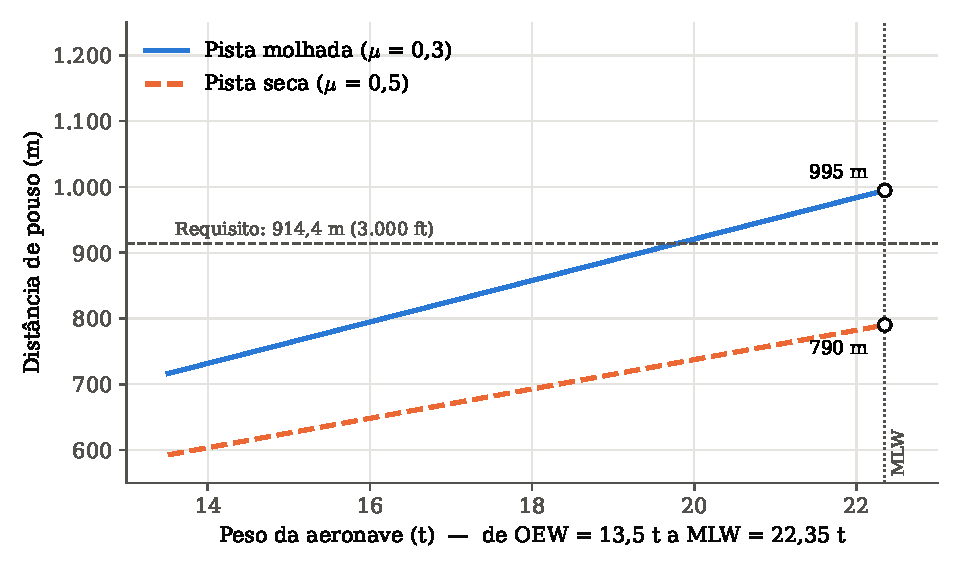
\includegraphics[width=0.7\textwidth]{images/fig7_11_pouso_peso.pdf}
    \caption{Distâncias de Pouso para a aeronave projetada.}
    \label{fig:distancias_pouso}
\end{figure}

Pode-se observar que a aeronave projetada apresentou um bom condicionamento para pistas padrão de pouso em voos regionais de transporte de passageiros/carga.

\section{Voo em Curva}

A avaliação das manobras em curva visa estabelecer o menor raio de giro ($R_{T}$) viável para a aeronave, garantindo não apenas a integridade estrutural, mas também a segurança durante os procedimentos de espera (\textit{holding}) e alinhamento típicos da aviação comercial em áreas de controle terminal. Tratando-se de uma curva coordenada e mantendo a altitude constante, o raio torna-se dependente do quadrado da velocidade aerodinâmica verdadeira ($V_{TAS}$) e da inclinação lateral aplicada ($\phi$), conforme a clássica relação:
\begin{equation}
    R_{T} = \frac{V_{TAS}^{2}}{g \cdot \tan(\phi)}
    \label{eq:raio_curva}
\end{equation}

Estipulou-se uma manobra a nível do mar, utilizando um fator de carga de segurança da ordem de $n = 1,3$. O ângulo de rolamento para curva coordenada \textit{bank angle} requisitado para suportar este esforço aparente obedece à equação geométrica:
\begin{equation}
    \phi = \arccos\left(\frac{1}{n}\right) = \arccos\left(\frac{1}{1,3}\right) \approx 39,71^{\circ}
\end{equation}

Sob a ótica dos requisitos de segurança, a velocidade durante a execução do giro deve apresentar uma folga de margem em relação ao estol, adotando-se o padrão de $1,3 \cdot V_{S0}$. Recorrendo à polar da aeronave em condição \textit{full-flap} ao nível do mar ($42,69 \text{ m/s}$), a velocidade tangencial demandada na trajetória de curva é dada por:
\begin{equation}
    V_{TAS} = 1,3 \times 42,69 \approx 55,5 \text{ m/s}
\end{equation}

Incorporando estas matrizes de dados na formulação central (Equação \ref{eq:raio_curva}), mapeia-se o raio operacional da máquina:
\begin{equation}
    R_{T} = \frac{(55,5)^{2}}{9,81 \cdot \tan(39,71^{\circ})}
\end{equation}
\begin{equation}
    R_{T} \approx 378,11 \text{ m}
\end{equation}


\section{Autonomia e Alcance}

O alcance (\textit{range}) e a autonomia (\textit{endurance}) foram estimados por meio das equações de Bréguet para aeronaves propelidas por hélice. Essas relações são utilizadas como uma aproximação da fase de cruzeiro, considerando voo reto e nivelado e parâmetros propulsivos representativos da condição analisada.

Como o consumo específico adotado é referido à potência no eixo, em $\mathrm{lb/(shp\cdot h)}$, utiliza-se a formulação de Bréguet baseada em potência, e não em tração.

O alcance no trecho de cruzeiro ($R$) é estimado pela Equação \ref{eq:breguet_alcance}:

\begin{equation}
    R = \frac{\eta_{\mathrm{prop}}}{c}
    \frac{C_L}{C_D}
    \ln\left(\frac{W_1}{W_2}\right)
    \label{eq:breguet_alcance}
\end{equation}

De forma análoga, a autonomia no trecho de cruzeiro é estimada pela Equação \ref{eq:breguet_autonomia}:

\begin{equation}
    E =
    \frac{\eta_{\mathrm{prop}}}{c}
    \frac{C_L^{3/2}}{C_D}
    \sqrt{2\rho S}
    \left(
    \frac{1}{\sqrt{W_2}}-
    \frac{1}{\sqrt{W_1}}
    \right)
    \label{eq:breguet_autonomia}
\end{equation}

Nessas equações, $\eta_{\mathrm{prop}}$ representa a eficiência propulsiva da hélice e $c$ o consumo específico de combustível referido à potência no eixo. Os termos $W_1$ e $W_2$ correspondem aos pesos da aeronave no início e no fim do trecho de cruzeiro, respectivamente.

Para a obtenção das curvas, cada altitude foi analisada separadamente, mantendo-se $\rho$ e o peso de referência constantes e variando-se a velocidade verdadeira. Para cada velocidade, o coeficiente de sustentação necessário ao voo nivelado foi calculado por:

\begin{equation}
    C_L = \frac{2W}{\rho V^2 S},
\end{equation}

e o coeficiente de arrasto foi obtido a partir da polar parabólica

\begin{equation}
    C_D = C_{D_0} + K C_L^2.
\end{equation}

Dessa forma, a razão $L/D=C_L/C_D$ varia com a velocidade, mesmo para uma mesma altitude. Assim, as Figuras \ref{fig:alcance_max} e \ref{fig:autonomia_max} representam varreduras de velocidade realizadas a altitude constante.

Com essas relações, foram obtidas as curvas de alcance e autonomia em função da velocidade verdadeira, apresentadas nas Figuras \ref{fig:alcance_max} e \ref{fig:autonomia_max}.

\begin{figure}[H]
    \centering
    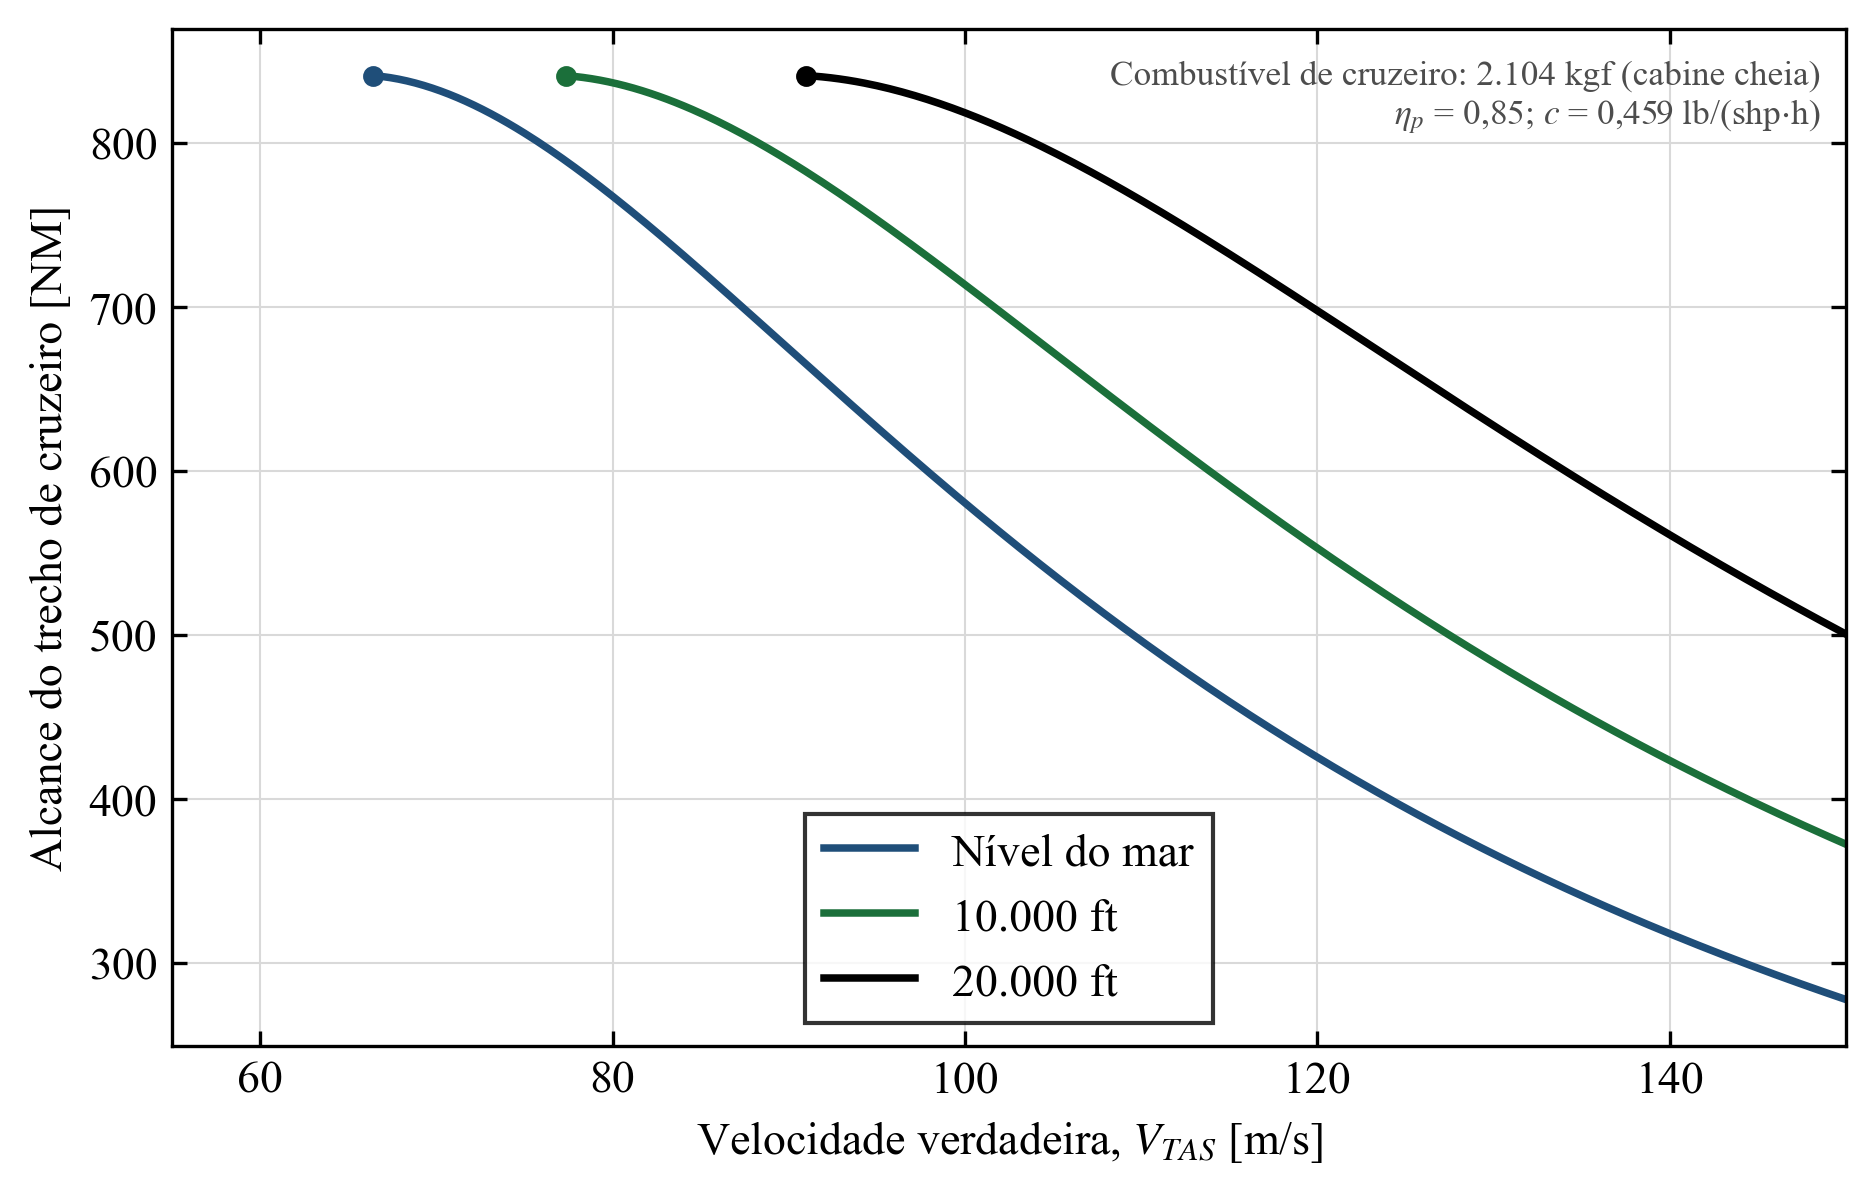
\includegraphics[width=0.8\textwidth]{images/alcance_max.png} 
    \caption{Alcance do trecho de cruzeiro em função da velocidade, com os 2.104~kgf de combustível de cruzeiro da missão com cabine cheia (Tabela~\ref{tab:combustivel_missao}), $\eta_{\mathrm{prop}} = 0{,}85$ e velocidades acima de $1{,}2\,V_S$.}
    \label{fig:alcance_max}
\end{figure}

\begin{figure}[H]
    \centering
    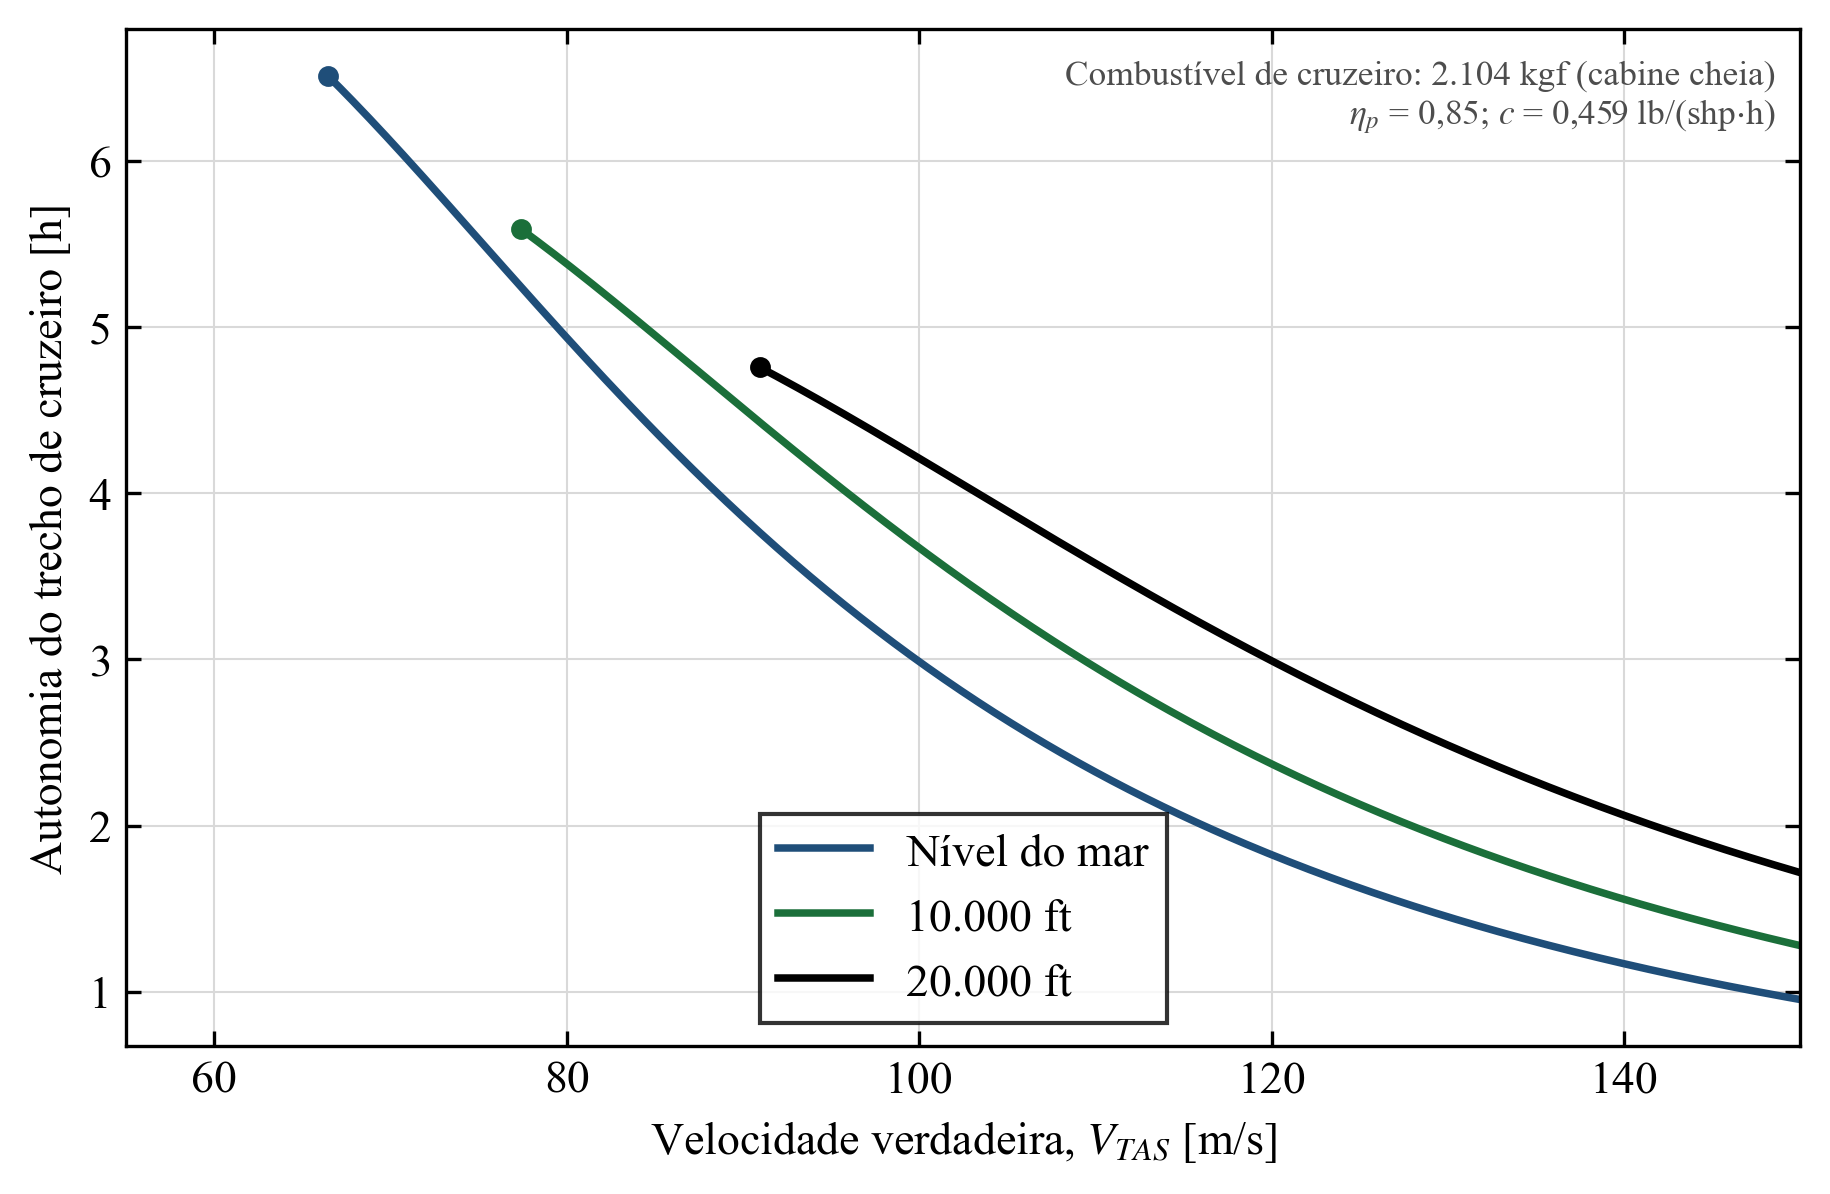
\includegraphics[width=0.8\textwidth]{images/autonomia_max.png}
    \caption{Autonomia do trecho de cruzeiro em função da velocidade, nas mesmas condições da Figura~\ref{fig:alcance_max}.}
    \label{fig:autonomia_max}
\end{figure}

Para uma polar parabólica, considerando peso e altitude constantes durante cada análise e assumindo $\eta_{\mathrm{prop}}$ e $c$ constantes, as velocidades teóricas associadas ao máximo alcance e à máxima autonomia são dadas por:

\begin{equation}
    V_{R_{max}} = \sqrt{\frac{2W}{\rho S}} \sqrt[4]{\frac{K}{C_{D_{0}}}}
\end{equation}
\begin{equation}
    V_{E_{max}} = \sqrt{\frac{2W}{\rho S}} \sqrt[4]{\frac{K}{3C_{D_{0}}}}
\end{equation}

O sumário dos limites estratégicos atingidos por esta configuração, mapeados ao nível do mar e na altitude operacional padrão de cruzeiro, encontra-se elucidado na Tabela \ref{tab:resultados_alcance}.

\begin{table}[H]
    \centering
    \caption{Resultados operacionais para autonomia e alcance máximos.}
    \vspace{0.2cm}
    \small
    \begin{tabular}{lccc}
        \toprule
        \textbf{Parâmetro} & \textbf{\makecell{Nível do Mar \\ (MSL)}} & \textbf{\makecell{Altitude de \\ 10000 ft}} & \textbf{\makecell{Altitude de Cruzeiro \\ (20000 ft)}} \\
        \midrule
        Vel. Máx Autonomia $V_{E_{max}}$ (m/s) & 50,3 & 58,5 & 68,9 \\
        Vel. Máx Alcance $V_{R_{max}}$ (m/s) & 66,2 & 77,0 & 90,7 \\
        \bottomrule
    \end{tabular}
    \label{tab:resultados_alcance}
    \caption*{Calculadas no MTOW, com $C_{D0} \approx 0,040$ e $K \approx 0,032$ ajustados à polar da Tabela 7.11.}
\end{table}

\subsection{Alcance da Missão de Projeto}
\label{sec:alcance_missao}

O alcance da missão de projeto foi calculado com a cabine cheia (64 passageiros com bagagem despachada) e decolagem no MTOW. Nessa condição o combustível a bordo é de 3.088~kgf (Tabela~\ref{tab:cg_pesos}), e não uma fração arbitrária da capacidade dos tanques. Esse combustível foi distribuído entre as fases da missão e as reservas IFR do requisito de alcance (alternativa a 100~NM e 45~minutos de espera, Seção~\ref{section:Requisitos}), com as seguintes hipóteses:

\begin{itemize}
    \item partida, táxi e decolagem com fração de peso de 0,995; descida e pouso com 0,997 cada;
    \item subida até 20.000~ft com o ângulo de $4{,}60^{\circ}$ do diagrama de missão, com o combustível obtido pela energia fornecida, $W\,\Delta h + D\,s$, com eficiência propulsiva de 0,80;
    \item cruzeiro a 20.000~ft pela Equação~\ref{eq:breguet_alcance}, com $c = 0{,}459~\mathrm{lb/(shp\cdot h)}$, $C_L$ constante na condição de máximo alcance limitada a $1{,}3\,V_S$ ($C_L = 0{,}89$, $V \approx 193$~kt TAS, $L/D = 13{,}8$ e $\eta_{\mathrm{prop}} = 0{,}85$, da tabela de eficiência da hélice em cruzeiro) e a polar de cruzeiro do CEA-VLM;
    \item descida em rampa de $3^{\circ}$, que percorre 116~km (Tabela~\ref{tab:fases_missao});
    \item reservas: alternativa a 100~NM em cruzeiro a 10.000~ft e espera de 45~minutos a 1.500~ft na velocidade de potência mínima.
\end{itemize}

\begin{table}[H]
    \centering
    \caption{Distribuição do combustível na missão de projeto (cabine cheia, MTOW).}
    \label{tab:combustivel_missao}
    \begin{tabular}{lcc}
        \toprule
        \textbf{Fase} & \textbf{Combustível [kgf]} & \textbf{Distância [NM]} \\
        \midrule
        Partida, táxi e decolagem & 113 & -- \\
        Subida até 20.000 ft & 246 & 41 \\
        Cruzeiro a 20.000 ft & 2.104 & 821 \\
        Descida e pouso & 121 & 63 \\
        Reserva: alternativa a 100 NM & 248 & -- \\
        Reserva: espera de 45 min & 256 & -- \\
        \midrule
        \textbf{Total} & \textbf{3.088} & \textbf{925} \\
        \bottomrule
    \end{tabular}
\end{table}

O alcance com a cabine cheia é de 925~NM, acima do requisito de 800~NM. Para voar exatamente 800~NM com as mesmas reservas são necessários 2.749~kgf de combustível, de modo que sobram cerca de 340~kgf. A aeronave pousa com cerca de 20.100~kgf, abaixo do MLW de 22.350~kgf. Com o combustível do trecho de cruzeiro voado na velocidade de potência mínima, a autonomia desse trecho é de cerca de 4,7~h (Tabela~\ref{tab:autonomia_alcance_cruzeiro}).

\begin{table}[H]
\centering
\caption{Alcance e autonomia da missão de projeto (cabine cheia, reservas IFR).}
\begin{tabular}{cc}
\hline
Alcance (NM) & Autonomia do trecho de cruzeiro (h) \\
\hline
925 & 4,7 \\
\hline
\end{tabular}
\label{tab:autonomia_alcance_cruzeiro}
\end{table}

\subsection{Diagrama de Carga Paga--Alcance}
\label{sec:carga_paga_alcance}

O diagrama de carga paga--alcance (Figura~\ref{fig:carga_paga_alcance}) mostra as combinações de passageiros, carga e combustível que respeitam o MTOW, o MZFW e a capacidade dos tanques, com o mesmo modelo de missão e as mesmas reservas da Tabela~\ref{tab:combustivel_missao}. Ele é definido pelos quatro pontos da Tabela~\ref{tab:pontos_carga_paga}:

\begin{itemize}
    \item \textbf{A}: carga paga máxima (6.080~kgf), limitada pelo MZFW, sem combustível de missão;
    \item \textbf{B}: carga paga máxima e combustível até o MTOW (3.088~kgf). Entre A e B, a carga paga é limitada pelo MZFW;
    \item \textbf{C}: tanques cheios (4.990~kgf) no MTOW, com a carga paga reduzida para 4.178~kgf. Entre B e C, cada quilograma-força de combustível a mais exige um a menos de carga paga, para não ultrapassar o MTOW;
    \item \textbf{D}: tanques cheios e nenhuma carga paga (voo de translado), decolando com 18.502~kgf.
\end{itemize}

Os pontos B e C são os limites da Tabela~\ref{tab:cg_cargapaga}. Em nenhum ponto o peso de pouso ultrapassa o MLW.

\begin{table}[H]
    \centering
    \caption{Pontos do diagrama de carga paga--alcance.}
    \label{tab:pontos_carga_paga}
    \small
    \begin{tabular}{cccccc}
        \toprule
        \textbf{Ponto} & \textbf{Carga paga} & \textbf{Combustível} & \textbf{Peso de decolagem} & \textbf{Alcance} & \textbf{Limitado por} \\
        \midrule
        A & 6.080 kgf & 0 kgf & 19.592 kgf & 0 NM    & MZFW \\
        B & 6.080 kgf & 3.088 kgf & 22.680 kgf & 925 NM  & MZFW e MTOW \\
        C & 4.178 kgf & 4.990 kgf & 22.680 kgf & 1.767 NM & MTOW e tanques \\
        D & 0 kgf & 4.990 kgf & 18.502 kgf & 2.265 NM & Tanques \\
        \bottomrule
    \end{tabular}
\end{table}

\begin{figure}[H]
    \centering
    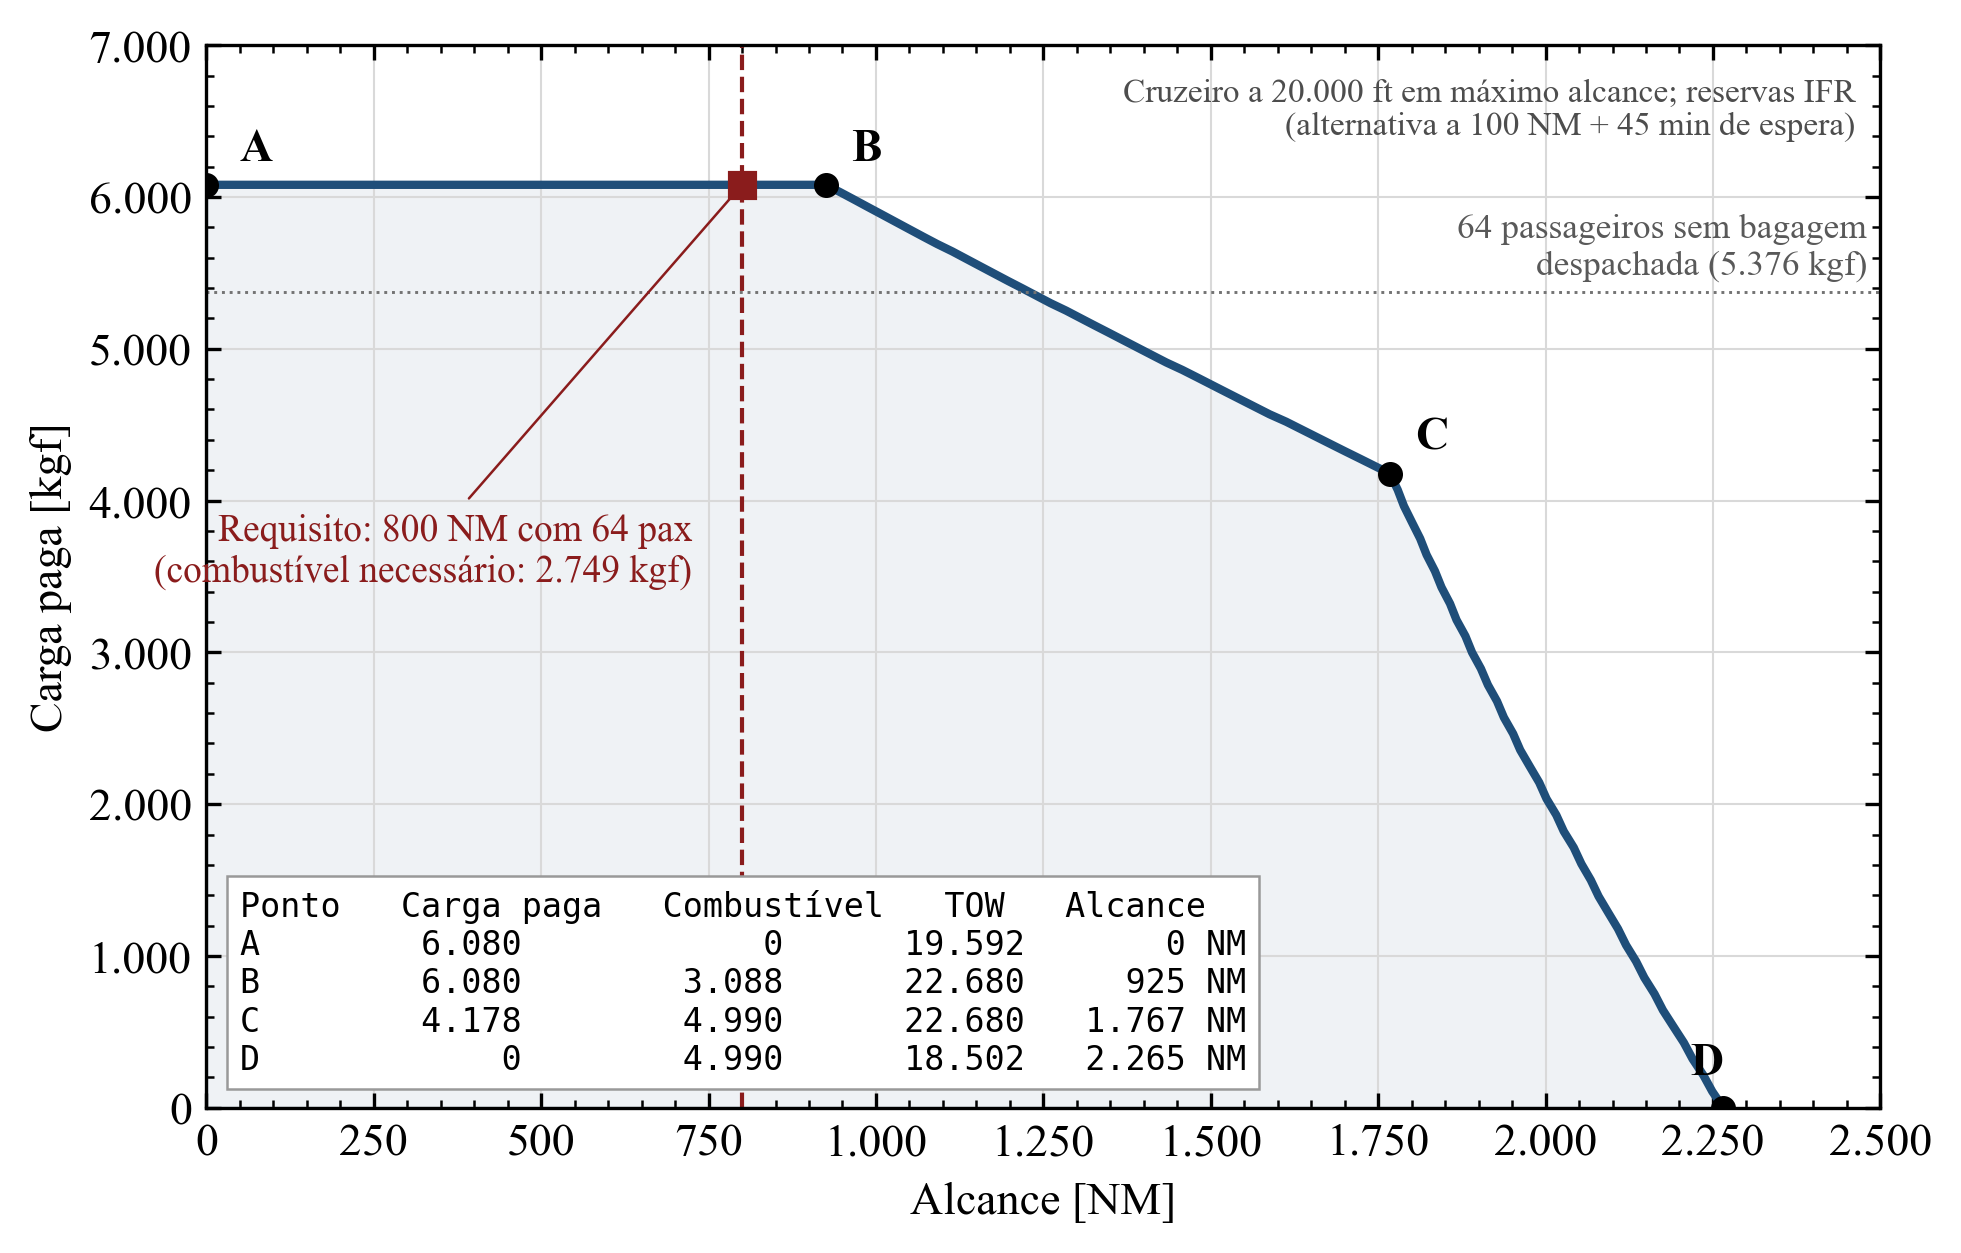
\includegraphics[width=0.95\textwidth]{images/Imagem - desempenho/carga_paga_alcance.png}
    \caption{Diagrama de carga paga--alcance com cruzeiro a 20.000~ft em máximo alcance e reservas IFR (alternativa a 100~NM e 45~min de espera). O quadrado marca o requisito de 800~NM com 64 passageiros.}
    \label{fig:carga_paga_alcance}
\end{figure}


\section{Envelope de Voo}


O envelope de voo é a representação gráfica que delimita a região operacional segura da aeronave em termos de altitude e velocidade verdadeira ($V_{TAS}$). A construção deste diagrama baseia-se na sobreposição dos limites aerodinâmicos (estol) e propulsivos (tração disponível versus necessária).

\subsection{Metodologia}

Para a obtenção do envelope de voo, foi desenvolvido um algoritmo computacional em MATLAB que realiza uma varredura iterativa em altitudes variando do nível do mar até o teto absoluto da aeronave. O procedimento de cálculo para cada altitude $h$ consiste nos seguintes passos:

\begin{enumerate}
    \item \textbf{Cálculo das Propriedades Atmosféricas:} Determinação da densidade do ar ($\rho$) conforme o modelo da Atmosfera Padrão (ISA).
    \item \textbf{Correção da Tração:} A curva de tração disponível ao nível do mar ($T_{SL}$) é corrigida pela razão de densidade ($\sigma = \rho / \rho_0$), assumindo-se um comportamento de motor aspirado:
    \begin{equation}
        T_{disp}(h, V) = T_{SL}(V) \cdot \sigma
    \end{equation}
    \item \textbf{Determinação das Potências:} Cálculo vetorial da Potência Disponível ($P_D = T_{disp} \cdot V$) e da Potência Requerida ($P_R = D \cdot V$) para uma faixa ampla de velocidades.
    \item \textbf{Obtenção dos Limites de Velocidade:} Identificação das interseções entre as curvas de $P_D$ e $P_R$.
\end{enumerate}

\subsection{Definição dos Limites do Envelope}

O envelope é delimitado por duas fronteiras principais:

\textbf{1. Limite Aerodinâmico (Esquerdo):} Definido pela velocidade de estol ($V_S$) na configuração limpa. Esta velocidade aumenta com a altitude devido à redução da densidade do ar, conforme a relação:
\begin{equation}
    V_S = \sqrt{\frac{2 \cdot W}{\rho \cdot S \cdot C_{L_{max}}}}
\end{equation}

\textbf{2. Limite Propulsivo (Direito e Teto):} Definido pela velocidade máxima ($V_{max}$) onde a potência disponível iguala a potência requerida.

Uma consideração crítica realizada no algoritmo é a determinação do limite mínimo de voo em grandes altitudes. Conforme a aeronave sobe, a curva de potência requerida se desloca para cima e para a direita (aumento do arrasto induzido e necessidade de maior $V_{TAS}$), enquanto a potência disponível decresce.

Em altitudes elevadas, a velocidade mínima sustentável pelo motor ($V_{min\_P}$) pode exceder a velocidade de estol aerodinâmico ($V_S$). Portanto, o limite esquerdo do envelope ($V_{esq}$) é definido computacionalmente pela lógica:
\begin{equation}
    V_{esq} = \max(V_S, V_{min\_P})
\end{equation}

Esta consideração explica a curvatura da fronteira esquerda do envelope em altitudes próximas ao teto, onde a aeronave entra no "segundo regime de comando" e a limitação torna-se propulsiva, e não mais puramente aerodinâmica.

\subsection{Resultados do Envelope}

A Figura \ref{fig:envelope_de_voo} apresenta o envelope de voo calculado no MTOW, com a área alar de 74,1~m$^2$ (a versão anterior desta análise usava 54,1~m$^2$, diferente da área alar de 74,1~m$^2$ do projeto). Observa-se que a região operacional se estreita com o ganho de altitude até convergir para um único ponto: o Teto Absoluto. Neste ponto, $V_{min} = V_{max}$, indicando que a aeronave possui apenas uma velocidade possível de voo nivelado e a razão de subida é nula.

\begin{figure}[H]
    \centering
    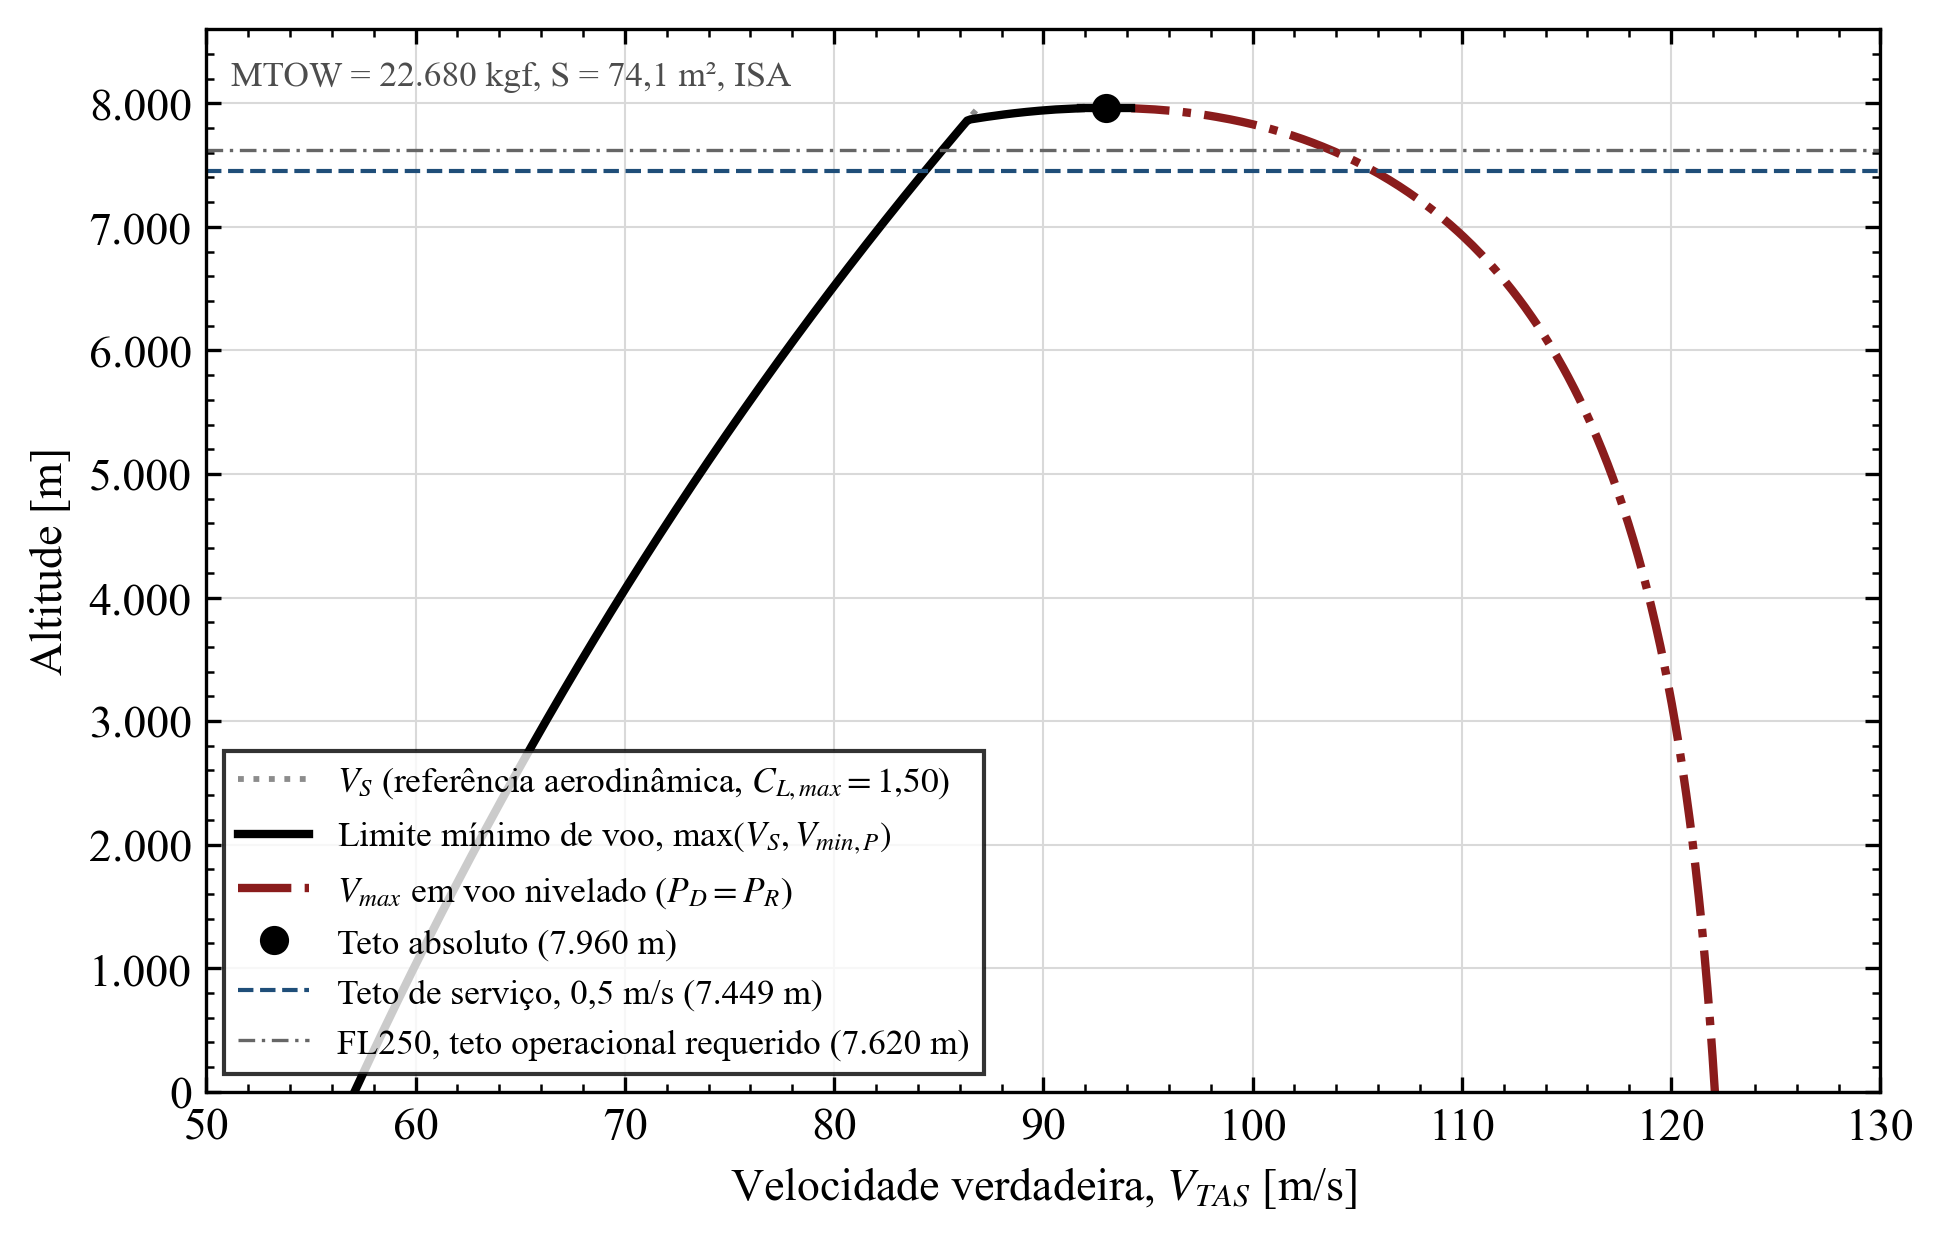
\includegraphics[width=0.9\linewidth]{images/Imagem - desempenho/envelope_voo.png}
    \caption{Envelope de voo no MTOW ($S = 74{,}1$~m$^2$, ISA): limite inferior de estol ou de potência, velocidade máxima em voo nivelado e tetos.}
    \label{fig:envelope_de_voo}
\end{figure}

Com os cálculos obteve-se um teto absoluto de 7.960~m (26.115~ft). A velocidade máxima em voo nivelado é de 122,1~m/s (237~kt) ao nível do mar e de 114,0~m/s (222~kt TAS) a 20.000~ft.

\subsection{Envelope de Operação}
\label{sec:envelope_operacao}

O envelope de operação (Figura~\ref{fig:envelope_operacao}) reúne, em altitude-pressão e velocidade verdadeira, os limites aerodinâmicos e propulsivos do envelope de voo e os limites estruturais e operacionais definidos para a certificação:

\begin{itemize}
    \item velocidade de estol 1~g com flaps recolhidos ($V_{S1}$, $C_{L,max} = 1{,}50$);
    \item velocidade máxima em voo nivelado, limitada pela potência disponível;
    \item velocidade máxima operacional $V_{MO}$, adotada igual a $V_C = 230$~kt EAS, já que o \S 25.1505 do 14 CFR Part 25 não permite $V_{MO}$ maior que $V_C$ (Seção~\ref{sec:cargas_vn});
    \item velocidade de mergulho de projeto $V_D = 288$~kt EAS (\S 25.335(b)), que não pode ser atingida em operação normal;
    \item teto de serviço, teto absoluto e o FL250 do requisito de teto operacional.
\end{itemize}

Abaixo de cerca de 2.000~ft a velocidade máxima em voo nivelado (237~kt EAS ao nível do mar) supera $V_{MO}$, e o limite à direita passa a ser estrutural. Acima disso, o limite à direita é a potência disponível. O teto de serviço de 24.438~ft fica 562~ft abaixo do FL250 requerido, de modo que o teto operacional certificável, no MTOW, fica limitado pelo teto de serviço. A faixa de cruzeiro a 20.000~ft vai de 193~kt TAS, na condição de máximo alcance, a 222~kt TAS, na potência máxima.

\begin{figure}[H]
    \centering
    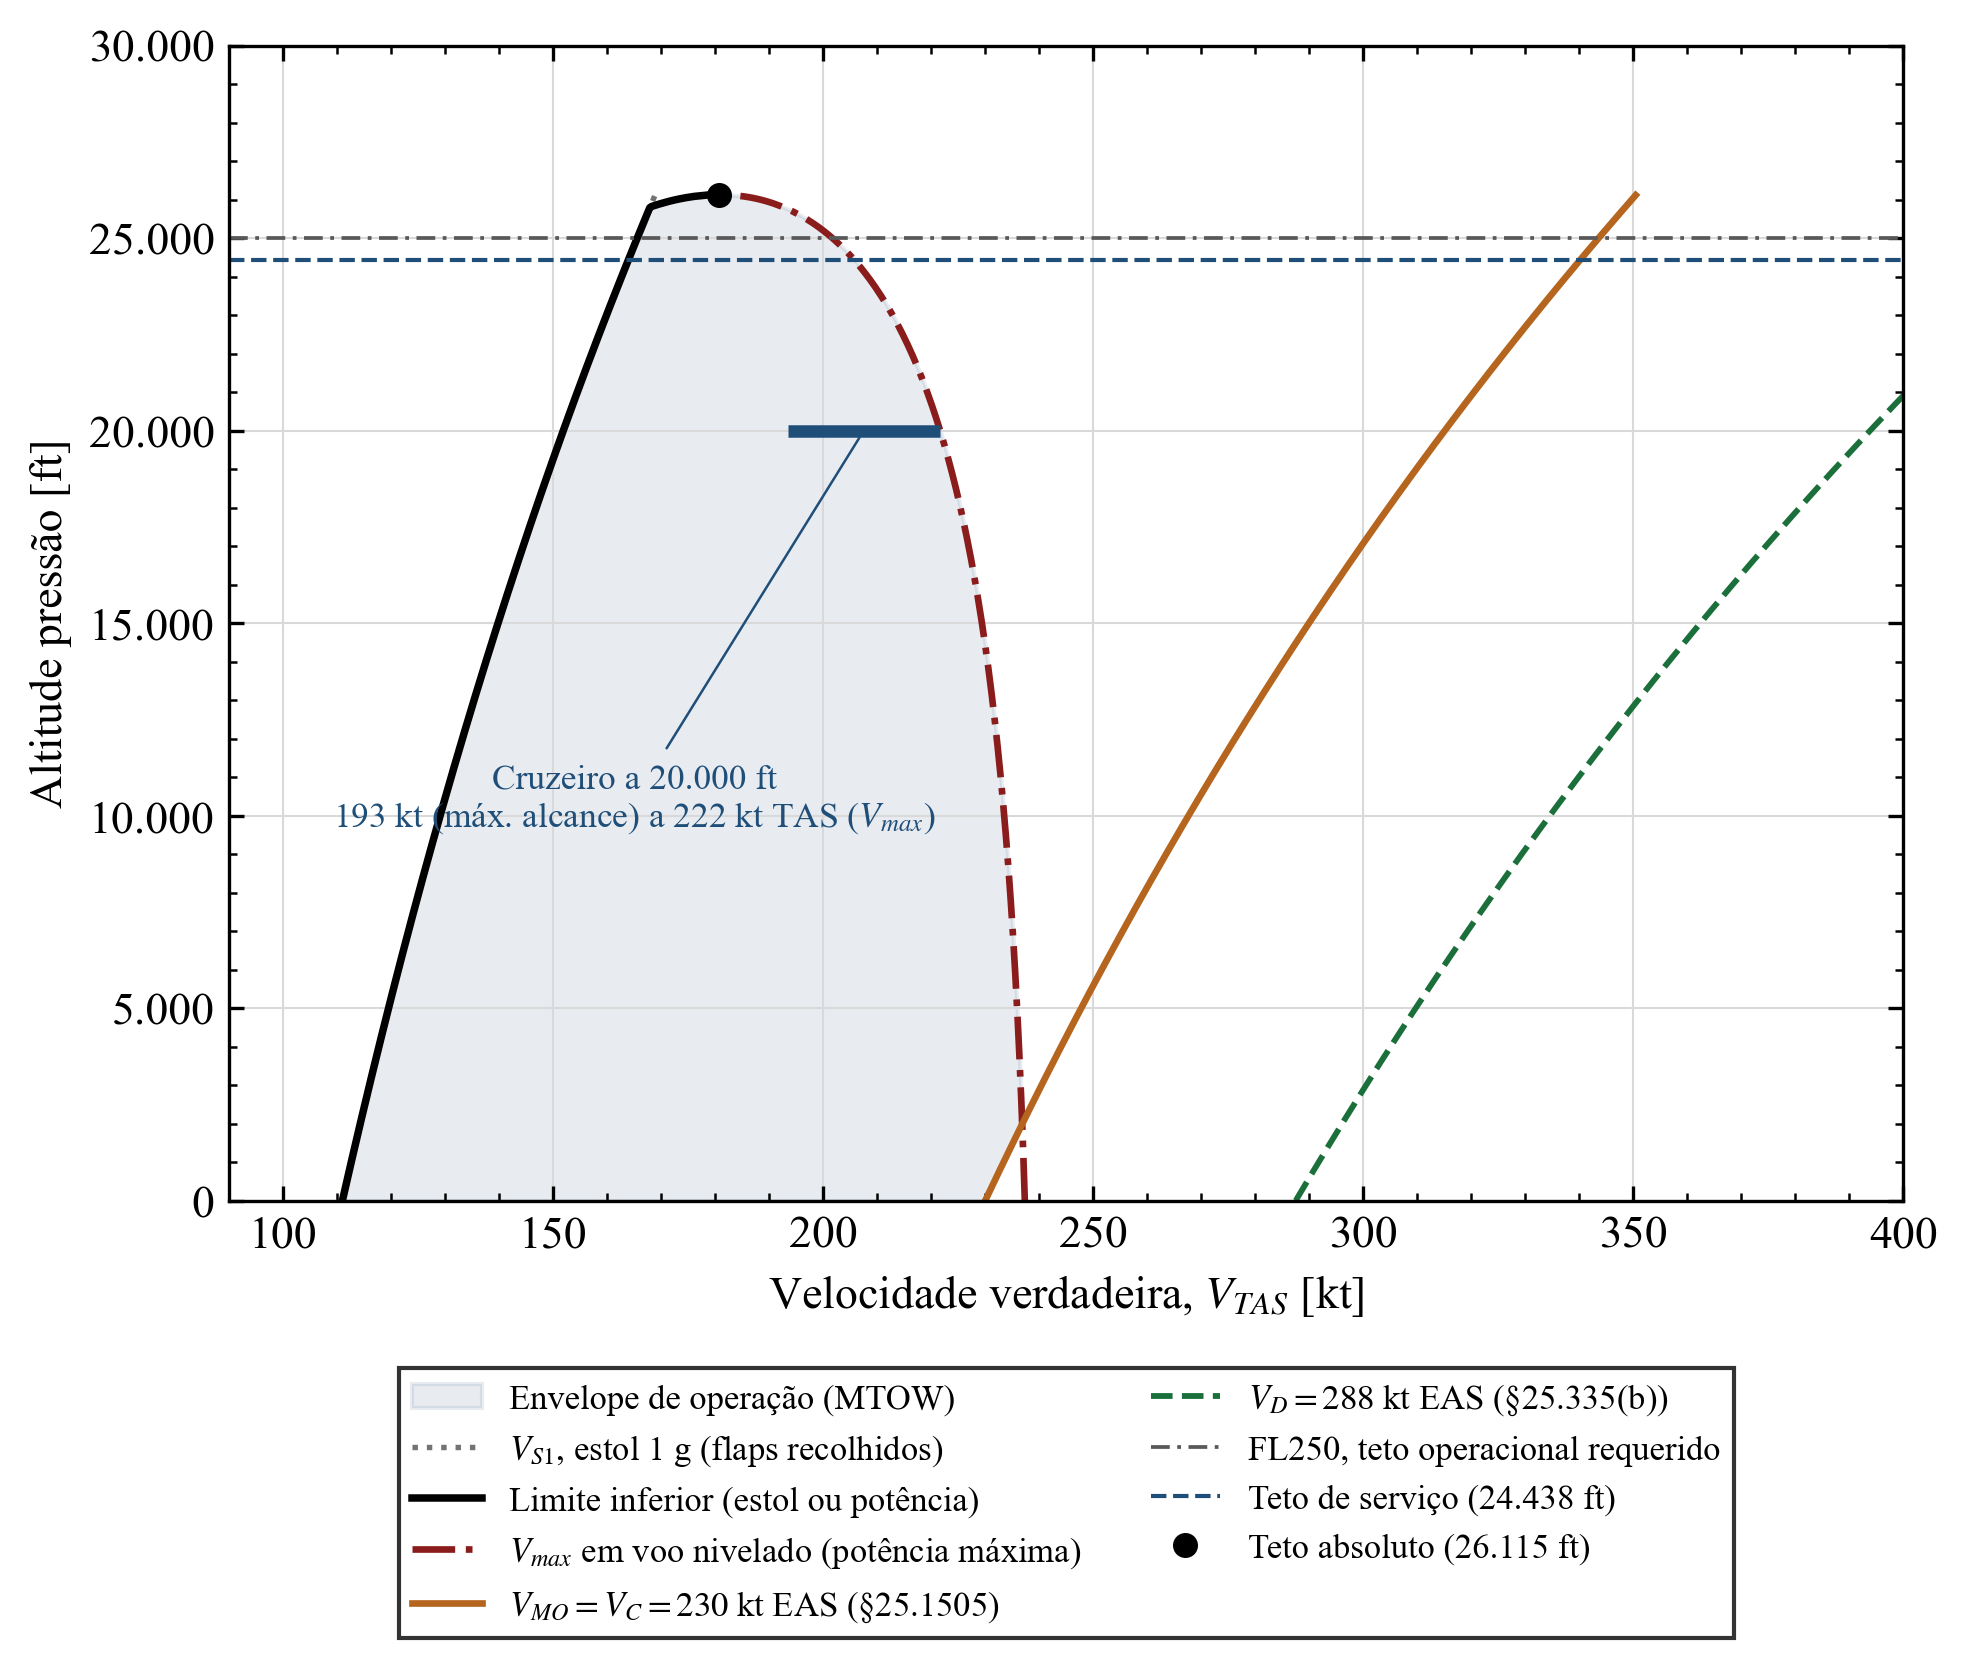
\includegraphics[width=0.95\textwidth]{images/Imagem - desempenho/envelope_operacao.png}
    \caption{Envelope de operação no MTOW: limites de estol, potência, $V_{MO} = V_C$ e $V_D$ (14 CFR Part 25), tetos de serviço e absoluto, FL250 requerido e faixa de cruzeiro a 20.000~ft.}
    \label{fig:envelope_operacao}
\end{figure}



\subsection{Desempenho de Subida}

A capacidade de subida da aeronave é determinada pelo excesso de potência específica (Excess Power). O algoritmo calculou a Razão de Subida ($RC$ - Rate of Climb) para cada velocidade dentro do vetor de análise através da equação:

\begin{equation}
    RC = \frac{P_{disp} - P_{req}}{W}
\end{equation}

Para cada altitude analisada, o código identificou o valor máximo dessa função ($RC_{max}$), que corresponde à melhor taxa de subida possível naquela condição atmosférica.

A Figura \ref{fig:desempenho_subida} ilustra a degradação da razão de subida máxima com o aumento da altitude. O ponto onde a curva intercepta o eixo horizontal (altitude) corresponde ao teto absoluto teórico, onde $RC_{max} = 0$. Para fins operacionais, destaca-se também o Teto de Serviço, definido como a altitude onde a razão de subida cai para 0,5 m/s (aproximadamente 100 ft/min).



\begin{figure}[H]
    \centering
    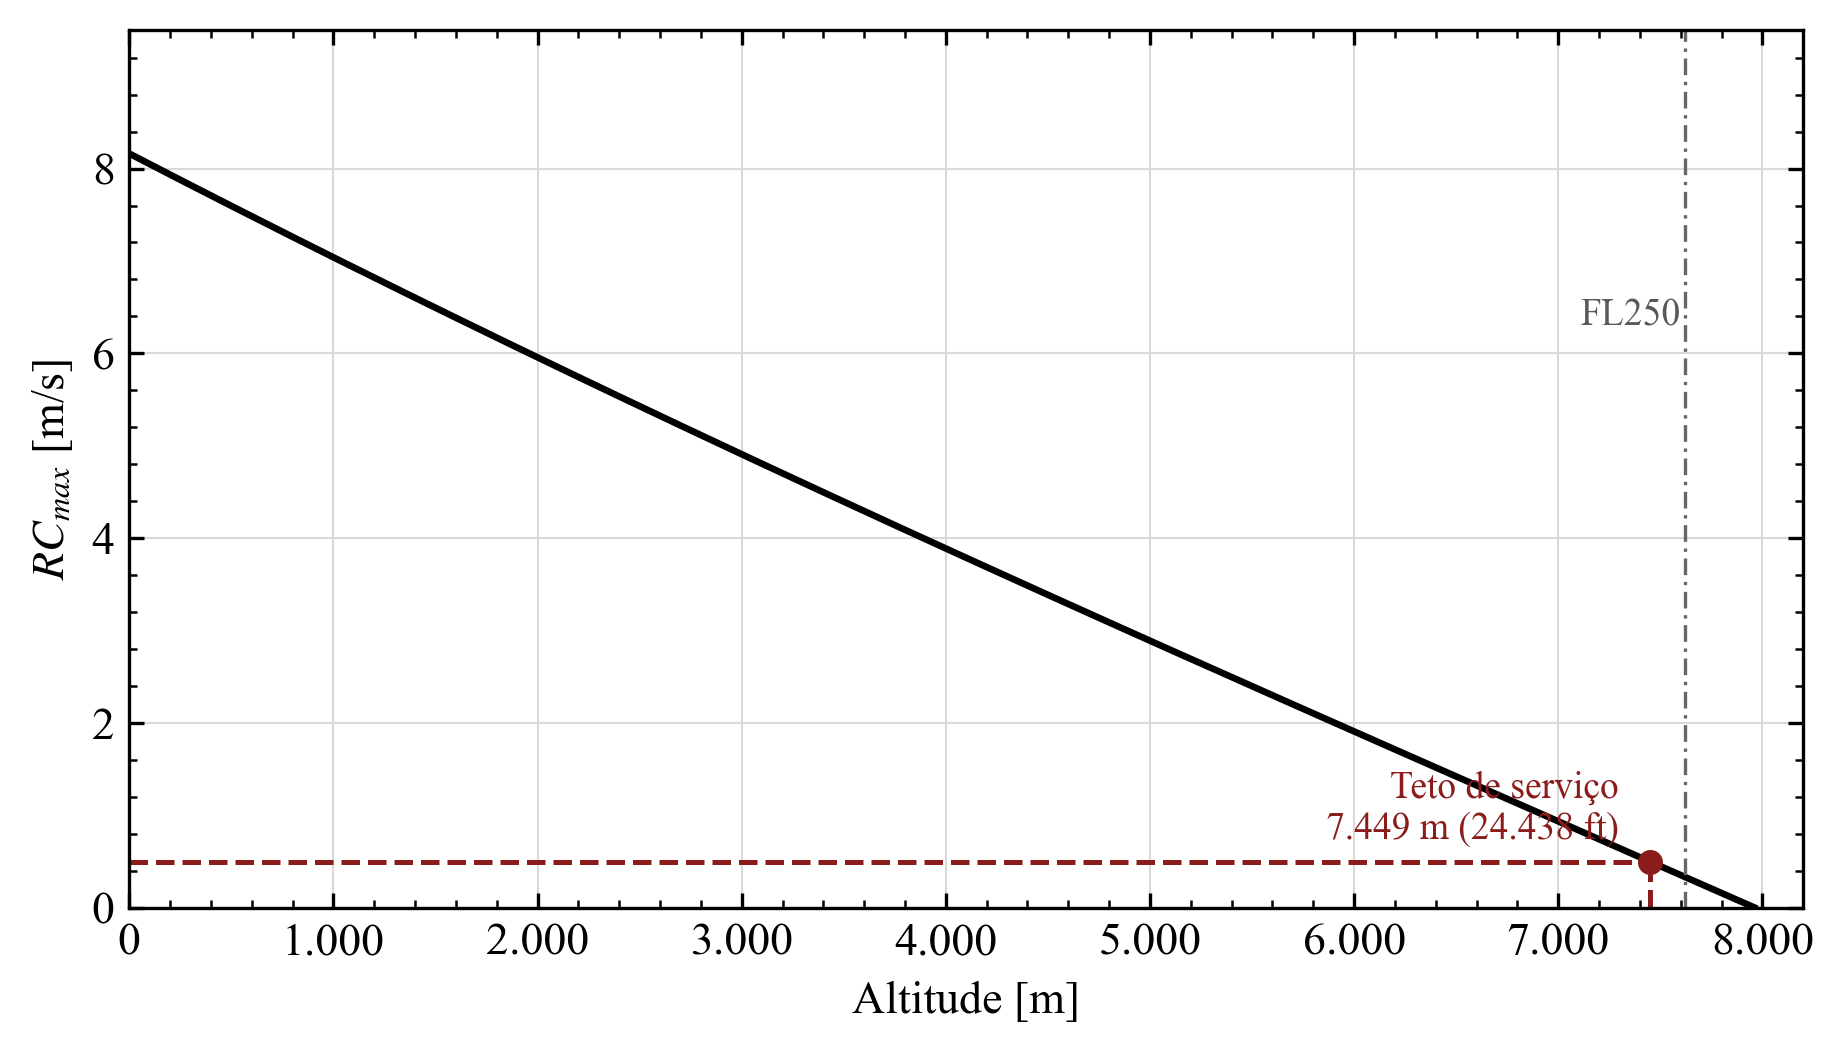
\includegraphics[width=0.9\linewidth]{images/Imagem - desempenho/desempenho_subida.png}
    \caption{Razão de subida máxima em função da altitude, no MTOW ($S = 74{,}1$~m$^2$).}
    \label{fig:desempenho_subida}
\end{figure}


Assim, obteve-se um teto de serviço de 7.449~m (24.438~ft). A 20.000~ft, a razão de subida máxima é de 1,81~m/s (356~ft/min).



\section{Diagrama de Missão}

O Diagrama de Missão representa o perfil de voo calculado para a aeronave em projeto, ilustrando a variação da altitude em função da distância horizontal percorrida desde a decolagem até o pouso completo.

Este perfil foi elaborado considerando as condições de Atmosfera Padrão (ISA), peso máximo de decolagem (MTOW) de 22.680 kgf e operação de pista ao nível do mar. A missão atende a operação baseando-se no alcance máximo estipulado de 800 NM (1.481,6 km), com a etapa de cruzeiro realizada no teto operacional de 20.000 pés.

\subsection{Parâmetros da Missão}

A Tabela \ref{tab:fases_missao} consolida as distâncias horizontais percorridas e as variações de altitude em cada segmento da missão. As distâncias de subida e descida foram projetadas no solo com base no ângulo geométrico de subida calculado ($\gamma \approx 4{,}60^{\circ}$) e numa rampa de aproximação padrão do sistema ILS ($3^{\circ}$).

\begin{table}[H]
    \centering
    \caption{Discriminação das fases da missão típica.}
    \label{tab:fases_missao}
    \vspace{0.2cm}
    \resizebox{\textwidth}{!}{%
    \begin{tabular}{llrrrr}
        \toprule
        \textbf{Fase} & \textbf{Segmento} & \textbf{Distância (m)} & \textbf{Distância (ft)} & \textbf{Alt. Inicial (ft)} & \textbf{Alt. Final (ft)} \\
        \midrule
        \textbf{1. Decolagem} & Corrida no Solo & 907{,}5 & 2.977 & 0 & 0 \\
                              & Transição até Obstáculo & 194{,}1 & 637 & 0 & 35 \\
        \midrule
        
        \textbf{2. Subida}    & \textit{Climb} contínuo & 75.580{,}0 & 247.967 & 35 & 20.000 \\
        \midrule
        
        \textbf{3. Cruzeiro}  & Voo Nivelado & 1.289.992{,}0 & 4.232.257 & 20.000 & 20.000 \\
        \midrule
        
        \textbf{4. Descida}   & Rampa de Planeio & 116.028{,}0 & 380.668 & 20.000 & 50 \\
        \midrule
       
        \textbf{5. Pouso}     & Aproximação e Arredondamento & 329{,}8 & 1.082 & 50 & 0 \\
                              & Corrida de Frenagem & 460{,}2 & 1.510 & 0 & 0 \\
    
        \bottomrule
    \end{tabular}
    }
\end{table}

\subsection{Descrição das Fases}

As características operacionais de cada etapa, ilustradas na Figura \ref{fig:diagrama_missao}, são descritas a seguir:

\begin{enumerate}
    \item \textbf{Decolagem:} A aeronave inicia a missão com uma corrida no solo  de 907,5 m até atingir a velocidade de rotação. Após a decolagem, considera-se uma distância horizontal de 194,1 m para o ganho de altura e ascensão em segurança até a altura do obstáculo padrão de 35 pés (\S25.113). A distância total de decolagem requerida é de aproximadamente 1.102 m.
    
    \item \textbf{Subida (\textit{Climb}):} A partir de 35 pés, a aeronave ascende até a altitude de cruzeiro de 20.000 pés. Sustentada pela potência excedente dos motores acoplados, a aeronave mantém um ângulo de trajetória de voo de $4{,}60^{\circ}$, percorrendo horizontalmente cerca de 75,5 km até atingir o nível de voo no ponto TOC (\textit{Top of Climb}).
    
    \item \textbf{Cruzeiro:} É a fase predominante da missão, onde a aeronave estabiliza em voo reto e nivelado sob regime de potência eficiente. A distância desta etapa é extraída do balanço total da missão, cobrindo quase 1.290 km para garantir o fechamento do alcance estipulado de 800 NM.
    
    \item \textbf{Descida:} Inicia-se no ponto ideal de descida TOD (\textit{Top of Descent}). Assumindo uma rampa de descida padrão de $3^{\circ}$ típica de voos comerciais de passageiros e carga, a aeronave percorre uma distância de solo de aproximadamente 116 km até interceptar a altitude do obstáculo da cabeceira (50 pés).
    
    \item \textbf{Pouso:} Compreende a aproximação aérea final descendo dos 50 pés, o arredondamento de 78 m para redução abrupta da razão de descida e o toque na pista (\textit{Touchdown}). Após o impacto, inicia-se a corrida de frenagem no solo de 460 m. A distância total da fase de pouso situa-se na margem segura de 790 m.
\end{enumerate}

\begin{figure}[H]
    \centering
        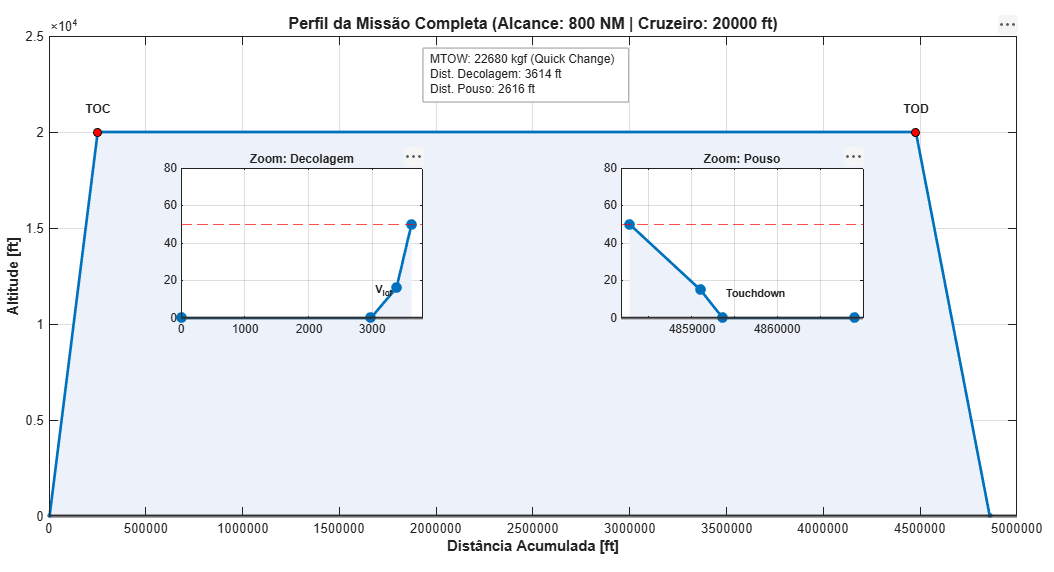
\includegraphics[width=1.0\textwidth]{images//Imagem - desempenho/diagrama de missão.png}
    \caption{Perfil de missão e trajetórias de pista (Altitude vs. Distância Acumulada) para a aeronave proposta.}
    \label{fig:diagrama_missao}
\end{figure}

\newpage
\section{Resumo dos Cálculos de Desempenho da Aeronave}

A tabela \ref{tab:resumo_desempenho} a seguir sumariza a maior parte dos cálculos e estimativas do desempenho da aeronave projetada. É interessante notar que os valores aqui calculados são satisfatoriamente competitivos para o mercado daquele tipo de missão que se pretende realizar com a presente aeronave.


\begin{table}[H]
    \centering
    \caption{Resumo de Desempenho da Aeronave}
    \label{tab:resumo_desempenho}
    \renewcommand{\arraystretch}{1.3} 
    
    % --- INÍCIO DO RESIZEBOX ---
    \resizebox{\textwidth}{!}{%
    \begin{tabular}{@{}llc@{}}
        \toprule
        \textbf{Categoria} & \textbf{Parâmetro} & \textbf{Valor de Projeto} \\
        \midrule
        
        \multirow{3}{*}{\textbf{Pesos e Capacidades}}
        & Peso Máximo de Decolagem (MTOW) & 22.680 kgf (50.000 lb) \\
        & Peso Máximo de Pouso (MLW) & 22.350 kgf (49.273 lb) \\
        & Peso Vazio Operacional (OEW) &
        13.512 kgf (29.789 lb) \\
        \midrule
        
        \multirow{2}{*}{\textbf{Motorização}}
        & Grupo Motopropulsor & 2x Pratt \& Whitney PW127M \\
        & Potência de Decolagem (por motor) & 2.475 shp \\
        \midrule
        
        \multirow{5}{*}{\textbf{Velocidades}}
        & Velocidade de Cruzeiro de Máximo Alcance (20.000 ft) & 193 kt TAS \\
        & Velocidade Máxima em Cruzeiro ($V_{max,cru}$) & 222 kt \\
        & Velocidade Máxima de Decolagem ($V_{max,TO}$) & 193,8 kt \\
        & Velocidade de Estol, flap 40° (MLW) & 82,4 kt \\
        & Razão de Subida Máxima para Cruzeiro ($RC_{max,cru}$) & 1,81 m/s \\
        \midrule
        
        \multirow{3}{*}{\textbf{Operação em Pista (MSL)}}
        & Distância Total de Decolagem & 1.102 m (3.614 ft) \\
        & Distância Física de Pouso & 790 m (2.592 ft) \\
        & Comprimento de Pista Balanceado (BFL) & 1620 m (5.315 ft) \\
        \midrule
        
        \multirow{4}{*}{\textbf{Limites de Missão}}
        & Alcance com Cabine Cheia e Reservas IFR & 925 NM (requisito: 800 NM) \\
        & Autonomia do Trecho de Cruzeiro (cabine cheia) & 4,7 horas \\
        & Teto de Serviço & 24.438 ft (7.449 m) \\
        & Teto Absoluto & 26.115 ft (7.960 m) \\
                
        \bottomrule
    \end{tabular}
    } % --- FIM DO RESIZEBOX ---
    
\end{table}
\chapter{Estabilidade}
\label{estabilidade}


\section{Forças Atuantes em Voo}

Para complementar a análise de estabilidade, apresentam-se a seguir duas representações
das forças atuantes sobre a aeronave em voo: um diagrama simplificado, destacando as
forças principais de sustentação, peso, tração e arrasto, e um diagrama complementar
que ilustra como essas forças se distribuem ao longo do comprimento da fuselagem.

\begin{figure}[H]
    \centering
    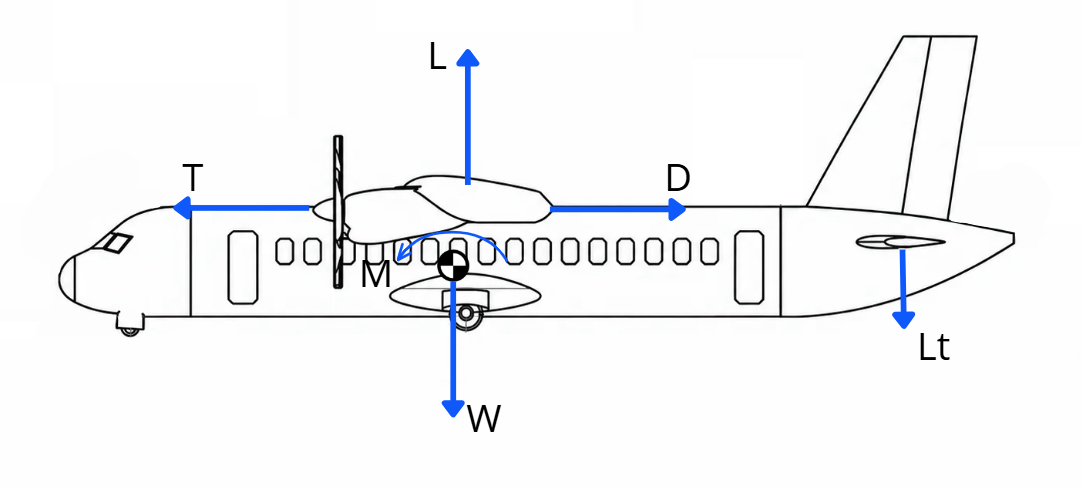
\includegraphics[width=0.92\textwidth]{Images-3-ProjetoDetalhado/CargaPontual.png}
    \caption{Representação simplificada das forças em voo.}
    \label{forcas_em_voo}
\end{figure}

\begin{figure}[H]
    \centering
    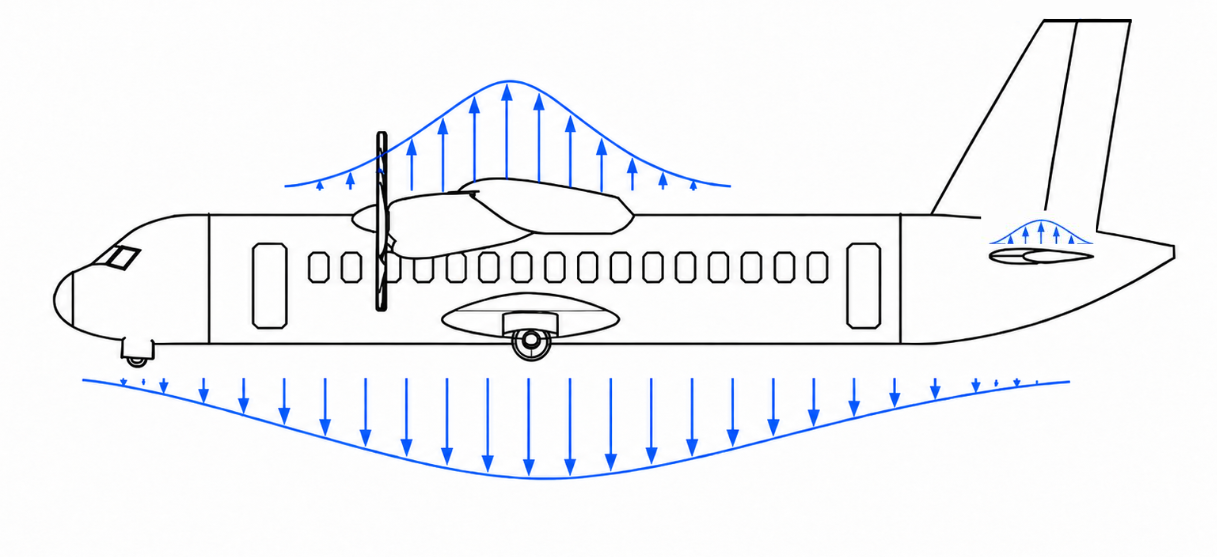
\includegraphics[width=0.92\textwidth]{Images-3-ProjetoDetalhado/CargaDistribuida.png}
    \caption{Representação simplificada das forças distribuídas ao longo da fuselagem.}
    \label{forca_distribuida}
\end{figure}




\section{Análise Preliminar da Estabilidade Longitudinal}

Com a determinação do envelope do centro de gravidade, foi feita uma análise inicial da estabilidade longitudinal da aeronave.



Para isso foi necessário obter as derivadas de estabilidade em torno de uma condição de equilíbrio. Utilizou-se novamente o software AVL para a obtenção desses parâmetros para uma condição de trimagem em cruzeiro da aeronave a uma altitude de 20000 ft.

%====================================================================
%  PONTO 2 -- Tabela de derivadas de estabilidade (inserida logo após
%  a apresentação da obtenção das derivadas no AVL)
%====================================================================

As principais derivadas de estabilidade longitudinal obtidas no AVL, para as duas posições extremas do centro de gravidade analisadas (dianteira e traseira), estão reunidas na Tabela~\ref{tab:derivadas_long} (as demais derivadas obtidas estão listadas nos anexos). Todas as derivadas angulares são expressas por radiano, e as derivadas em relação às velocidades angulares ($C_{L_q}$, $C_{m_q}$) foram convertidas da forma adimensional a partir da expressão ($q\bar{c}/2V$). A posição do centro de gravidade é dada em fração da corda média aerodinâmica ($h_{CG}$), medida a partir do bordo de ataque da CMA, e a margem estática (SM) foi calculada por $\text{SM} = -C_{m_\alpha}/C_{L_\alpha}$, definição equivalente a $\text{SM} = X_{np}/\bar{c} - h_{CG}$ desde que $X_{np}$ seja referido à mesma origem de $h_{CG}$ (o AVL retorna $X_{np}$ a partir do ponto de referência do arquivo \texttt{.avl}, fixado em $c/4$ da CMA, exigindo a correção de $+0{,}25\bar{c}$ ao compará-lo com $h_{CG}$).

\begin{table}[H]
    \centering
    \caption{Derivadas de estabilidade longitudinal e parâmetros associados para as condições extremas de CG, obtidas no AVL a 20000 ft de altitude.}
    \begin{tabular}{|l|c|c|}
       \hline
       \textbf{Parâmetro} & \textbf{CG dianteiro} & \textbf{CG traseiro} \\
       \hline
       $h_{CG}$ (\%  $\bar{c}$)        & $0{,}179$   & $0{,}459$  \\
       \hline
       Margem estática (SM)              & $0{,}587$   & $0{,}307$  \\
       \hline
       $C_{L_\alpha}$ [rad$^{-1}$]       & $5{,}816$   & $5{,}816$  \\
       \hline
       $C_{L_q}$ [rad$^{-1}$]            & $14{,}907$  & $11{,}649$ \\
       \hline
       $C_{m_\alpha}$ [rad$^{-1}$]       & $-3{,}412$  & $-1{,}783$ \\
       \hline
       $C_{m_q}$ [rad$^{-1}$]            & $-42{,}955$ & $-37{,}783$\\
       \hline
    \end{tabular}
    \label{tab:derivadas_long}
\end{table}

Antes da análise modal, verificou-se a coerência física dos sinais das derivadas dominantes em arfagem. Em ambas as condições de CG, $C_{m_\alpha} < 0$ confirma estabilidade estática longitudinal (com margem estática positiva em todo o envelope), e $C_{m_q} < 0$ confirma amortecimento positivo em arfagem. Como esperado, a rigidez estática $C_{m_\alpha}$ e a margem estática são maiores na condição de CG dianteiro, tornando a aeronave mais estável (porém menos manobrável) nessa configuração, e menores na condição traseira, que representa o caso crítico de estabilidade do envelope.

Por fim, com o fim de simplificação de análise, foi feito desacoplamento do movimento longitudinal com o látero-direcional. Dessa forma, as variáveis de estado $\vec{x}_{long}$ e entradas $\vec{u}_{long}$ que descrevem o movimento são:

\begin{equation}
    \vec{x} = \begin{bmatrix} V \\ \alpha \\ \theta \\ q \\ h   \end{bmatrix} \qquad \vec{u} = \begin{bmatrix}
        \eta \\ \delta_t \\
    \end{bmatrix}
\end{equation}

Dessa forma, o sistema dinâmico linearizado pode ser descrito da forma:

\begin{equation}
\dot{\vec{x}} = A_{long} \ \vec{x} + B_{long} \ \vec{u}
\end{equation}

Onde matrizes $A_{long}$ e $B_{long}$ são obtidas a partir dos autovalores do sistema de equações diferencias, que também podem ser encontradas no apêndice.

Para fins de auxilio de cálculo, foi utilizado o MATLAB para a obtenção das matrizes e, consequentemente, dos modos longitudinais e seus polos. Os polos podem ser observados na Fig. \ref{polos}. O movimento longitudinal se apresentou ser dinamicamente estável em todo o intervalo do CG.

%====================================================================
%  PONTO 3 -- Excitação por doublet (inserida logo após a descrição do
%  modelo Simulink e do doublet aplicado)
%====================================================================

Para a simulação, foi feito um modelo dinâmico da aeronave no aplicativo do SIMULINK. Os resultados para a simulação podem ser encontrados no anexo.

\subsection{Dados de Massa e Inércia Empregados}

%====================================================================
%  PONTO 6 -- Dados de massa e inércia / aproximação dos momentos de
%  inércia
%====================================================================

A linearização e a simulação dinâmica exigem, além das derivadas aerodinâmicas, os dados de massa e do tensor de inércia da aeronave. A massa adotada corresponde ao peso máximo de decolagem (MTOW) de $22\,680$~kg. Como a aeronave possui plano de simetria longitudinal ($XZ$), os produtos de inércia $I_{xy}$ e $I_{yz}$ foram considerados nulos, restando os momentos principais $I_{xx}$, $I_{yy}$ e $I_{zz}$ (e, eventualmente, $I_{xz}$).

Na fase atual do projeto, ainda não se dispõe de uma distribuição detalhada de massa da estrutura e dos sistemas que permita o cálculo direto do tensor de inércia por integração. Por esse motivo, os momentos de inércia foram estimados pelo método dos raios de giração, abordagem usual em projeto preliminar, na qual cada momento de inércia é escrito em função da massa da aeronave, de uma dimensão característica e de um raio de giração adimensional $R$, conforme:

\begin{equation}
    I_{xx} = \frac{b^2 \, m \, R_x^2}{4}, \qquad
    I_{yy} = \frac{l_f^2 \, m \, R_y^2}{4}, \qquad
    I_{zz} = \frac{(b + l_f)^2 \, m \, R_z^2}{4}
    \label{eq:inercia_giracao}
\end{equation}

onde $m$ é a massa da aeronave, $b$ a envergadura, $l_f$ o comprimento da fuselagem, e $R_x$, $R_y$ e $R_z$ os raios de giração adimensionais associados, respectivamente, aos eixos de rolamento, arfagem e guinada. A lógica física por trás de cada dimensão característica reflete a distribuição predominante de massa em cada eixo: o momento de inércia em rolamento ($I_{xx}$) é dominado pela distribuição ao longo da envergadura $b$; o momento em arfagem ($I_{yy}$) pela distribuição ao longo do comprimento da fuselagem $l_f$; e o momento em guinada ($I_{zz}$), por envolver simultaneamente a distribuição em ambas as direções, é associado a uma dimensão combinada $(b + l_f)$. Os raios de giração adimensionais foram adotados a partir de valores típicos tabelados para aeronaves de mesma categoria.

Os valores resultantes empregados na análise estão reunidos na Tabela~\ref{tab:inercia}.

\begin{table}[H]
    \centering
    \caption{Massa e momentos de inércia estimados da aeronave.}
    \begin{tabular}{|l|c|}
       \hline
       \textbf{Parâmetro} & \textbf{Valor} \\
       \hline
       Massa (MTOW)            & $22\,680$ kg \\
       \hline
       $I_{xx}$                & $5{,}32 \times 10^{5}$ kg$\cdot$m$^2$ \\
       \hline
       $I_{yy}$                & $3{,}22 \times 10^{5}$ kg$\cdot$m$^2$ \\
       \hline
       $I_{zz}$                & $3{,}26 \times 10^{6}$ kg$\cdot$m$^2$ \\
       \hline
       $I_{xy} = I_{xz} = I_{yz}$ & $0$ \\
       \hline
    \end{tabular}
    \label{tab:inercia}
\end{table}

Cabe ressaltar que essa estimativa, embora adequada para uma análise preliminar de estabilidade, carrega incerteza significativa, uma vez que depende dos raios de giração adotados de referências externas e não da distribuição real de massa da aeronave em projeto. Os momentos de inércia influenciam diretamente o amortecimento e a frequência dos modos dinâmicos (em especial o curto período, fortemente dependente de $I_{yy}$), de modo que esses valores deverão ser refinados em fases posteriores do projeto, à medida que a distribuição de massa estrutural e de sistemas for detalhada.


\subsection{Excitação dos Modos por Doublet}

A excitação dos modos longitudinais foi feita por meio de um \textit{doublet} que consiste em um pulso de deflexão positiva imediatamente seguido por um pulso de deflexão negativa de mesma amplitude, retornando ao valor de trimagem ao final. Essa forma de entrada concentra a energia da excitação em torno de uma faixa estreita de frequência, sendo particularmente adequada para excitar predominantemente o modo de interesse.

A amplitude foi mantida pequena ($1^\circ$ de deflexão) de modo a preservar a validade da hipótese de pequenas perturbações, sobre a qual o modelo linearizado se fundamenta. A largura de cada pulso foi dimensionada de forma a ser da ordem da metade do período do modo de curto período, concentrando assim a excitação na sua frequência natural; o modo de longo período (fugóide), por possuir período muito mais elevado, é excitado de forma secundária pela perturbação inicial e observado na resposta livre subsequente, após o decaimento do transiente de curto período. Vale observar que, por ser uma entrada simétrica que retorna ao trim, o \textit{doublet} pouco altera a velocidade de equilíbrio, característica desejável para a observação do curto período, no qual a velocidade permanece aproximadamente constante.

\begin{figure}[H]
    \centering
    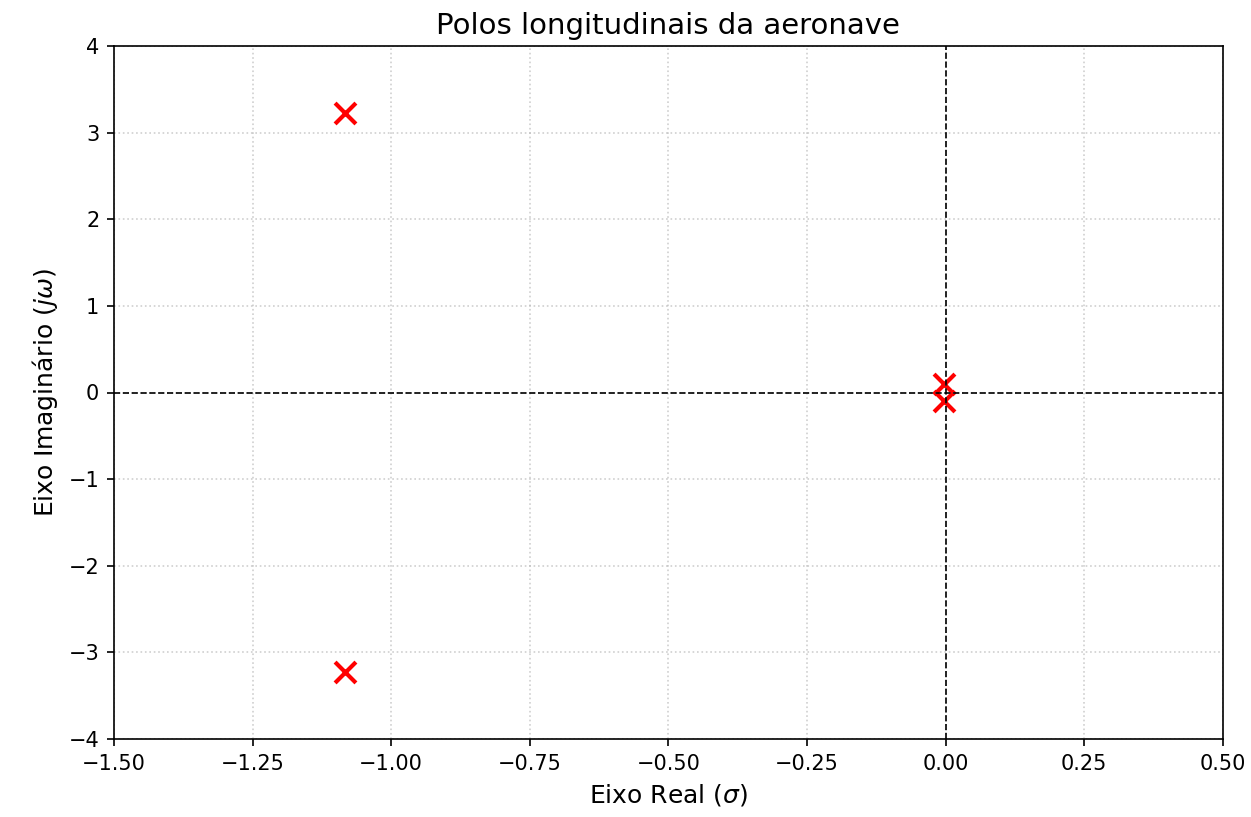
\includegraphics[width=0.5\linewidth]{Polos_projetos.png}
    \caption{Polos para o movimento longitudinal da aeronave.}
    \label{polos}
\end{figure}

\begin{figure}[H]
    \centering
    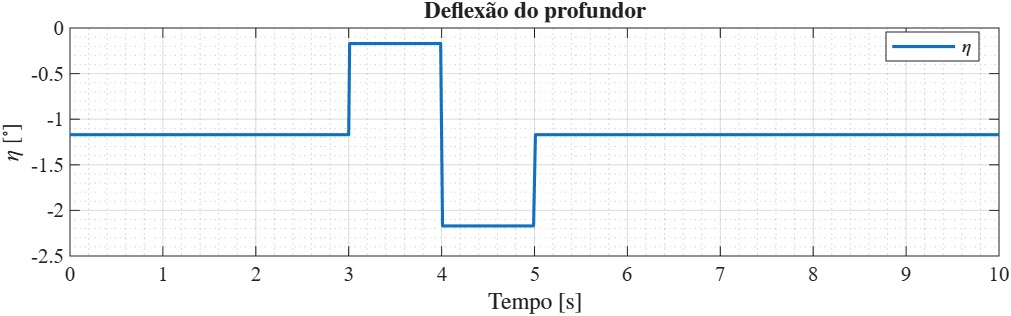
\includegraphics[width=0.5\linewidth]{images/doublet_eta.jpeg}
    \caption{Doublet aplicado no profundor}
    \label{doublet}
\end{figure}


\subsection{Modo Curto Período}

O modo curto período da aeronave tem as seguintes propriedades:

\begin{table}[H]
    \centering
    \caption{Características do curto período.}
    \begin{tabular}{|c|c|}
       \hline
       Polos  & $-1,0835 \pm 3,2287i$ \\
       \hline
       Frequência natural ($\omega_n$) & $3,4057$ rad/s \\
       \hline
       Taxa de amortecimento ($\zeta_{d}$) & $0,3182$\\
       \hline
       Período ($T$) & $1,9460$ s \\
       \hline
       Tempo de decaimento ($t_{1/2}$) & $0,6397$ s \\
       \hline
       Tempo de acomodação 2\% ($t_{s}$) & $3,6916$ s\\
       \hline
    \end{tabular}
    \label{curto_periodo}
\end{table}

O curto período da aeronave apresenta uma alta taxa de amortecimento e um pequeno período, o que auxilia a difícil percepção desse modo pelo piloto. O valor de $\zeta_d$ para o curto período está dentro do previsto na norma militar americana MIL-F-8785C para aeronaves do tipo. Nas Figuras \ref{curto_tras} e \ref{curto_dian} pode ser observado, para as condições traseira e dianteira do CG, a evolução no curto período para os ângulos $\alpha$, $\theta$ e $\gamma$. Demais gráficos podem ser encontrados no anexo.


\begin{figure}[H]
    \centering
    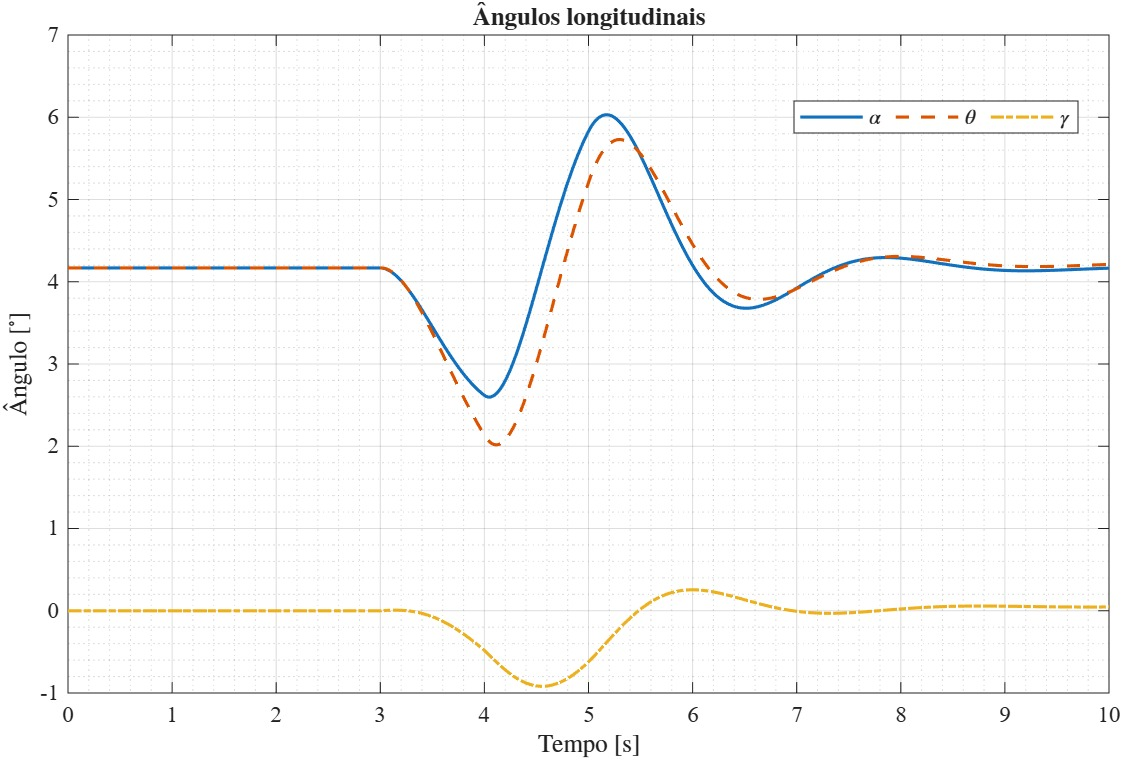
\includegraphics[width=\textwidth]{images/Imagem - desempenho/angulos_curto_CG_traseiro.jpeg}
    \caption{Condição de CG traseiro para o curto período.}
    \label{curto_tras}
\end{figure}

\begin{figure}[H]
    \centering
    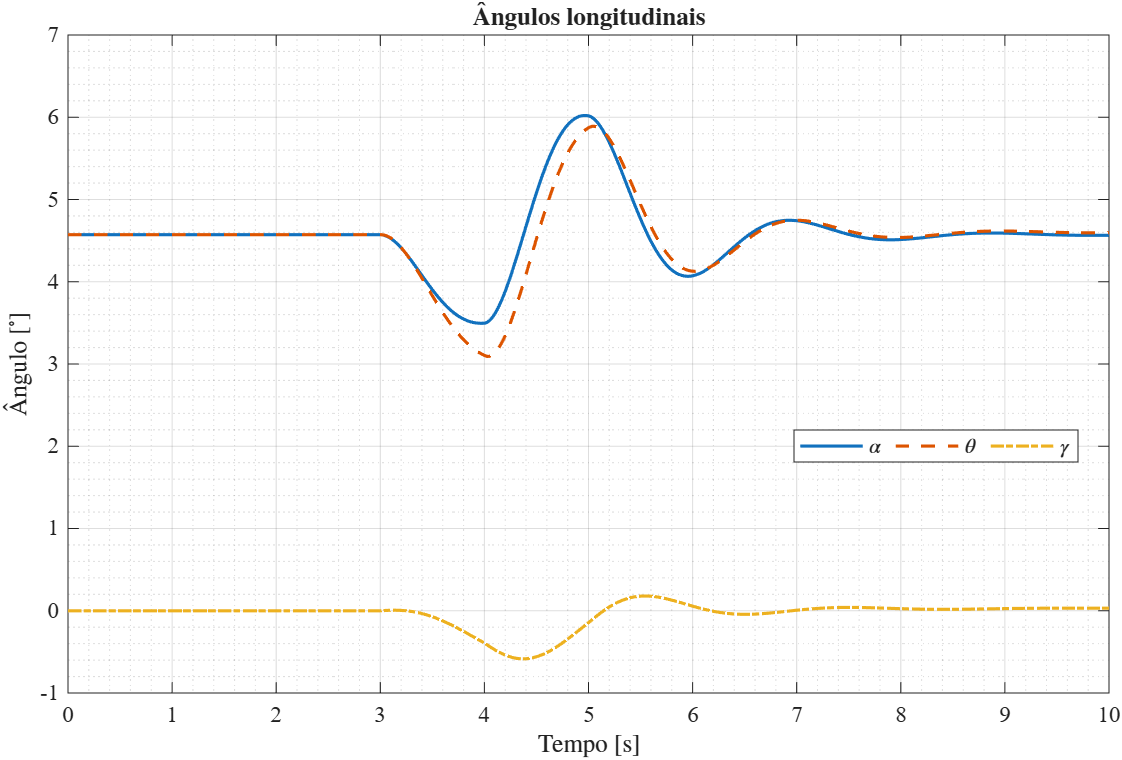
\includegraphics[width=\textwidth]{images/Imagem - desempenho/angulos_CG_dianteiro.png}
    \caption{Condição de CG dianteiro para o curto período.}
    \label{curto_dian}
\end{figure}






\subsection{Modo Longo Período}

%Dados fugóide

O modo longo período ou fugóide da aeronave tem as seguintes propriedades:

\begin{table}[H]
    \centering
    \caption{Características do longo período.}
    \begin{tabular}{|c|c|}
       \hline
       Polos  & $-0.0030 \pm 0.1018i$ \\
       \hline
       Frequência natural ($\omega_n$) & $0,1018$ rad/s \\
       \hline
       Taxa de amortecimento ($\zeta_{d}$) & $0,0291$\\
       \hline
       Período ($T$) & $61,7479$ s \\
       \hline
       Tempo de decaimento ($t_{1/2}$) & $234$ s \\
       \hline
       Tempo de acomodação 2\% ($t_{s}$) & $1350$ s\\
       \hline
    \end{tabular}
    \label{longo_periodo}
\end{table}

O modo longo período apresenta um amortecimento extremamente baixo (mesmo para os padrões da fugóide), fazendo com que a aeronave oscile muito tempo até retornar a condição de equilíbrio. Entretanto, o período também é de magnitude considerável o que ajuda a não percepção desse movimento, fazendo com que o baixo amortecimento não seja problemático. A aeronave consta dentro das especificações da norma MIL-F-8785C para aeronaves desse tipo. Nas Figuras \ref{longo_tras} e \ref{longo_dian} pode ser observado para ambos limites do CG a resposta da velocidade e altitude ao longo período. Gráficos das demais variáveis estão apresentados no anexo.


\begin{figure}[H]
    \centering
    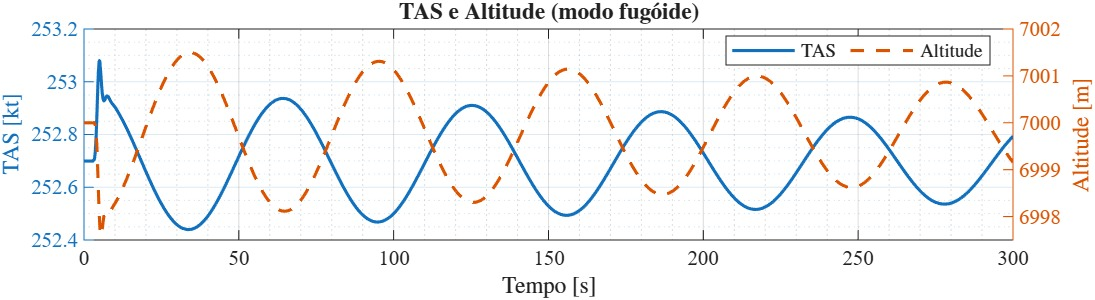
\includegraphics[width=\textwidth]{images/h_longo_CG_trazeiro.jpeg}
    \caption{Condição de CG traseiro para o longo período.}
    \label{longo_tras}
\end{figure}

\begin{figure}[H]
    \centering
    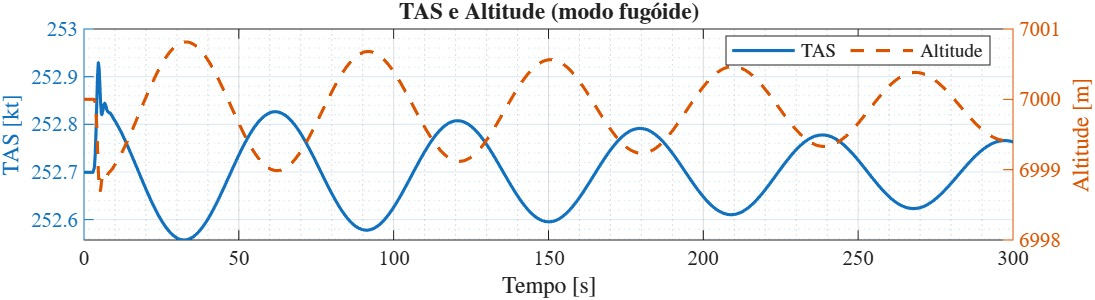
\includegraphics[width=\textwidth]{images/h_longo_CG_dianteiro.jpeg}
    \caption{Condição de CG dianteiro para o longo período.}
    \label{longo_dian}
\end{figure}

%====================================================================
%  PONTO 5 -- Validação cruzada simulação x linearização (inserida
%  após a apresentação dos dois modos, antes das conclusões)
%====================================================================

\subsection{Validação Cruzada entre a Linearização e a Simulação Não-linear}

Os modos longitudinais foram caracterizados por duas vias independentes, que se validam mutuamente. Os valores de frequência natural, amortecimento e período apresentados nas Tabelas~\ref{curto_periodo} e \ref{longo_periodo} foram obtidos analiticamente, a partir dos autovalores da matriz $A_{long}$ resultante da linearização do modelo no ponto de equilíbrio. Esses parâmetros não dependem da integração no tempo, sendo determinados unicamente pelo ponto de trimagem.

Como verificação independente, a resposta temporal obtida na simulação não-linear no SIMULINK foi confrontada com esses valores, obtendo resultados muito próximos da simulação linearizada. A concordância entre as duas abordagens, uma analítica e outra numérica não-linear, confere confiança ao modelo linear empregado e indica que a linearização captura adequadamente a dinâmica longitudinal da aeronave na vizinhança da condição de cruzeiro analisada.



\subsection{Conclusões}

A aeronave é caracterizada como dinamicamente estável em voo de cruzeiro em uma condição de voo reto nivelado, com características dos modos de longo e curto período que se adéquam à norma MIL-F-8785C para seu tipo. Para uma análise mais profunda de qualidade de voo é necessário avaliar a estabilidade látero direcial. Por fim, apesar das normas demonstrarem uma boa ideia sobre a validação das características dos modos longitudinais, uma avaliação completa dos modos longitudinais é feita em partes mais avançadas dor projeto, com dados de testes de modelos e ensaios em voo.



\chapter{Análise de Cargas}
\label{cap:analise_cargas}

\section{Representação dos carregamentos}
\label{sec:representacao_carregamentos}

A Figura~\ref{fig:forcas_aeronave} apresenta as principais forças e o momento aerodinâmico atuantes na aeronave, enquanto a Figura~\ref{fig:cargas_distribuidas} representa esquematicamente as cargas distribuídas na asa, na empenagem horizontal e ao longo da fuselagem. Esses esquemas ilustram os carregamentos considerados na análise, cujas condições de aplicação são definidas a partir do diagrama V--n e utilizadas no dimensionamento estrutural.

\begin{figure}[H]
    \centering
    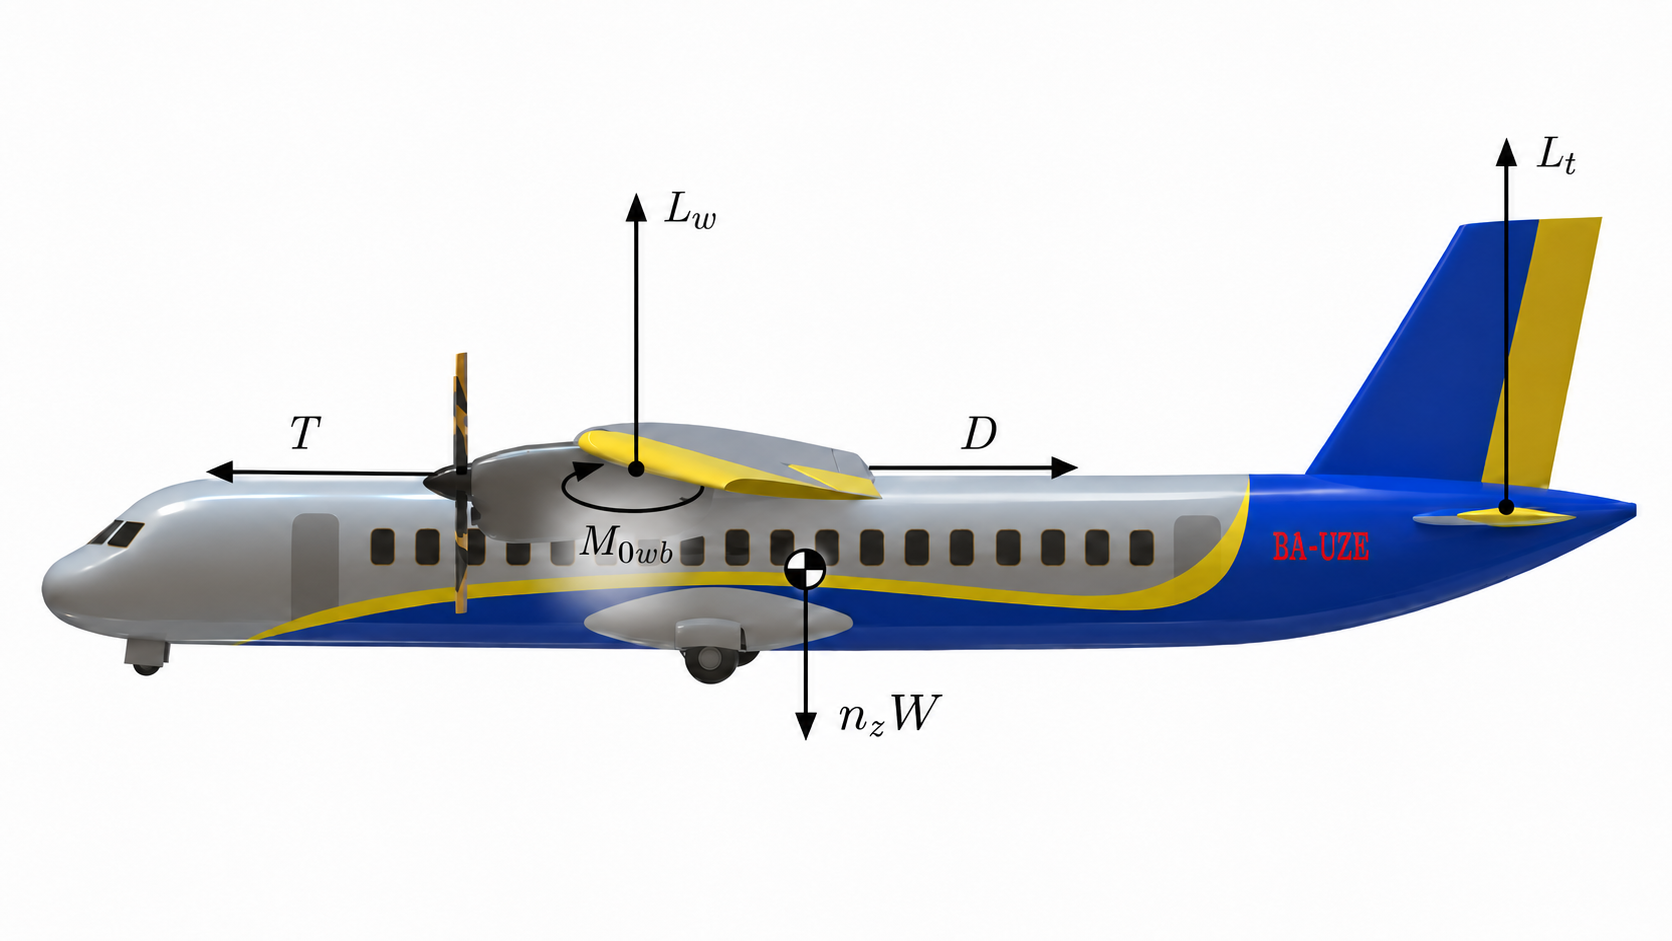
\includegraphics[width=0.85\textwidth]{images/cargas/Diagrama técnico de forças em aeronave.png}
    \caption{Principais forças e momento aerodinâmico atuantes na aeronave.}
    \label{fig:forcas_aeronave}
\end{figure}

\begin{figure}[H]
    \centering
    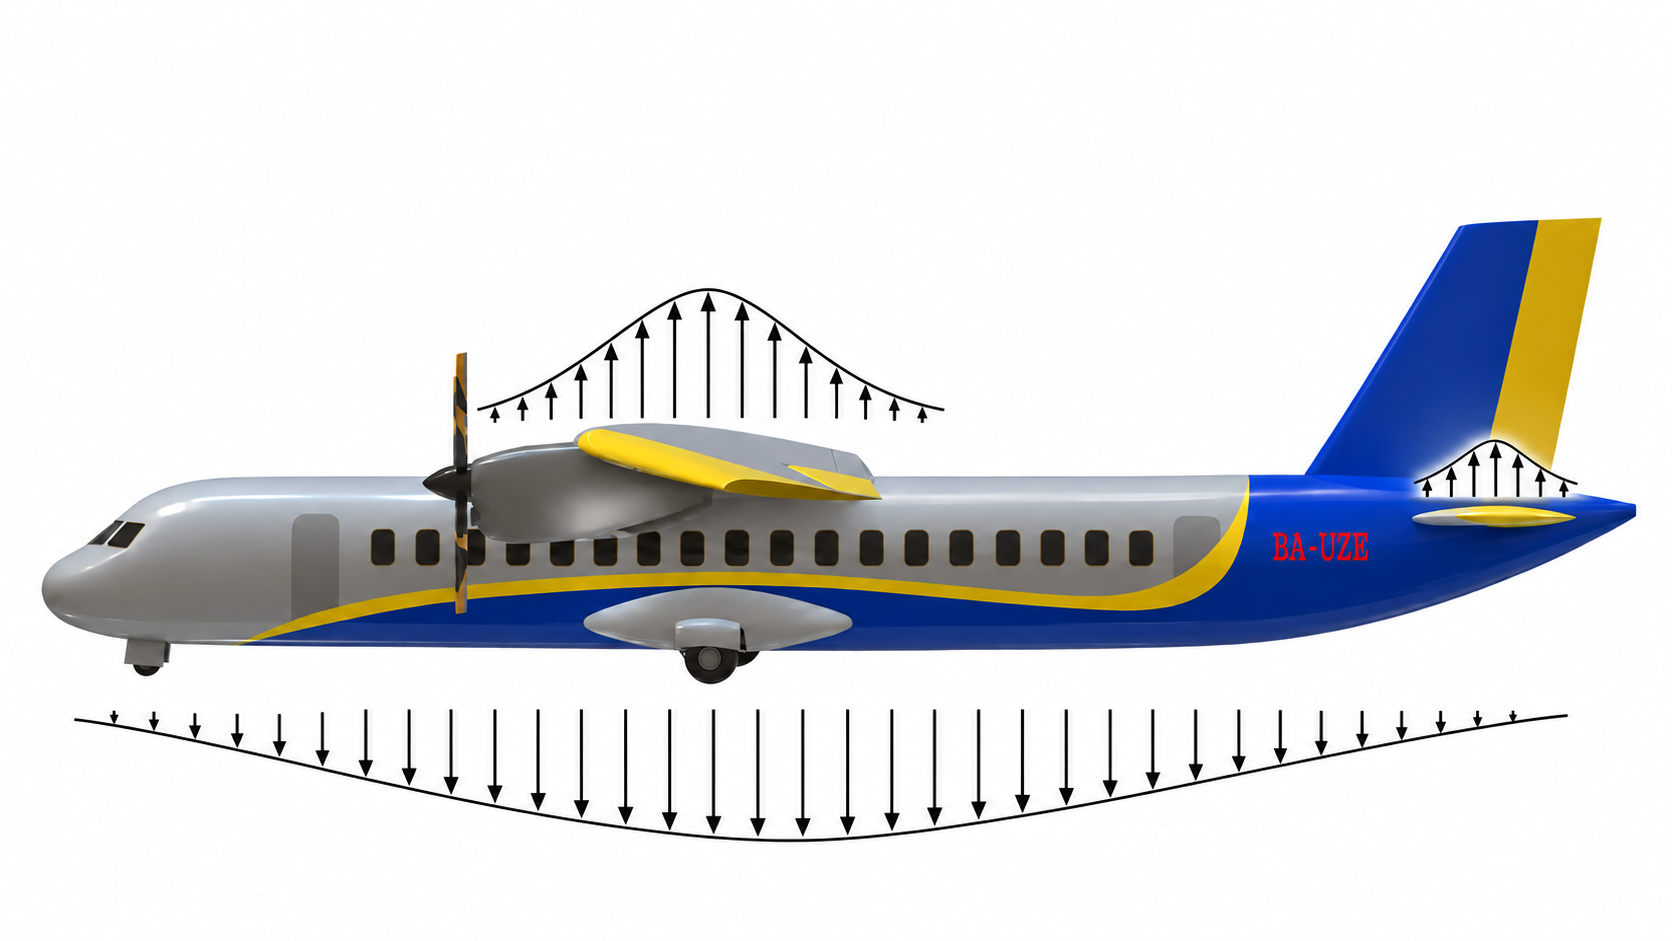
\includegraphics[width=0.85\textwidth]{images/cargas/Aeronave com diagramas de cargas distribuídas.png}
    \caption{Distribuição esquemática de cargas na aeronave.}
    \label{fig:cargas_distribuidas}
\end{figure}

\section{Diagrama V--n}
\label{sec:cargas_vn}

O diagrama V-n foi construído conforme o 14 CFR Part 25. As velocidades de projeto, em velocidade
equivalente, foram obtidas pelo \S 25.335 a partir do MTOW, da área alar $S = 74{,}1$~m$^2$ e dos
$C_{L_{max}}$ de cada configuração (1,50 limpo; 1,88 com flap de 10°; 2,69 com flap de 40°). Como os
valores de $V_C$ e $V_D$ adotados anteriormente eram inferiores aos mínimos da norma, foram
utilizados $V_C = 230$~kt ($V_C \geq V_B + 1{,}32\,U_{ref}$) e $V_D = 288$~kt ($V_C/V_D \leq 0{,}8$).
Os fatores de carga limite de manobra são $+2{,}5$ e $-1{,}0$ com flaps recolhidos (\S 25.337) e
$+2{,}0$ com flaps baixados (\S 25.345). As cargas de rajada foram estimadas pelo modelo quase-estático
de Pratt, com o fator de alívio $K_g$ do \S 25.335(d) e a velocidade de rajada de projeto do
\S 25.341(a) ($U_{de} = 41{,}1$~ft/s entre $V_B$ e $V_C$ ao nível do mar e 25~ft/s com flaps). As
Figuras~\ref{fig:vn_manobra} a \ref{fig:vn_projeto_20k} apresentam, respectivamente, o envelope de
manobra com flaps recolhidos e baixados, as linhas de rajada e o envelope de projeto resultante ao nível
do mar e a 20\,000~ft. Em todas as condições o envelope de manobra é o crítico.

\begin{figure}[H]
    \centering
    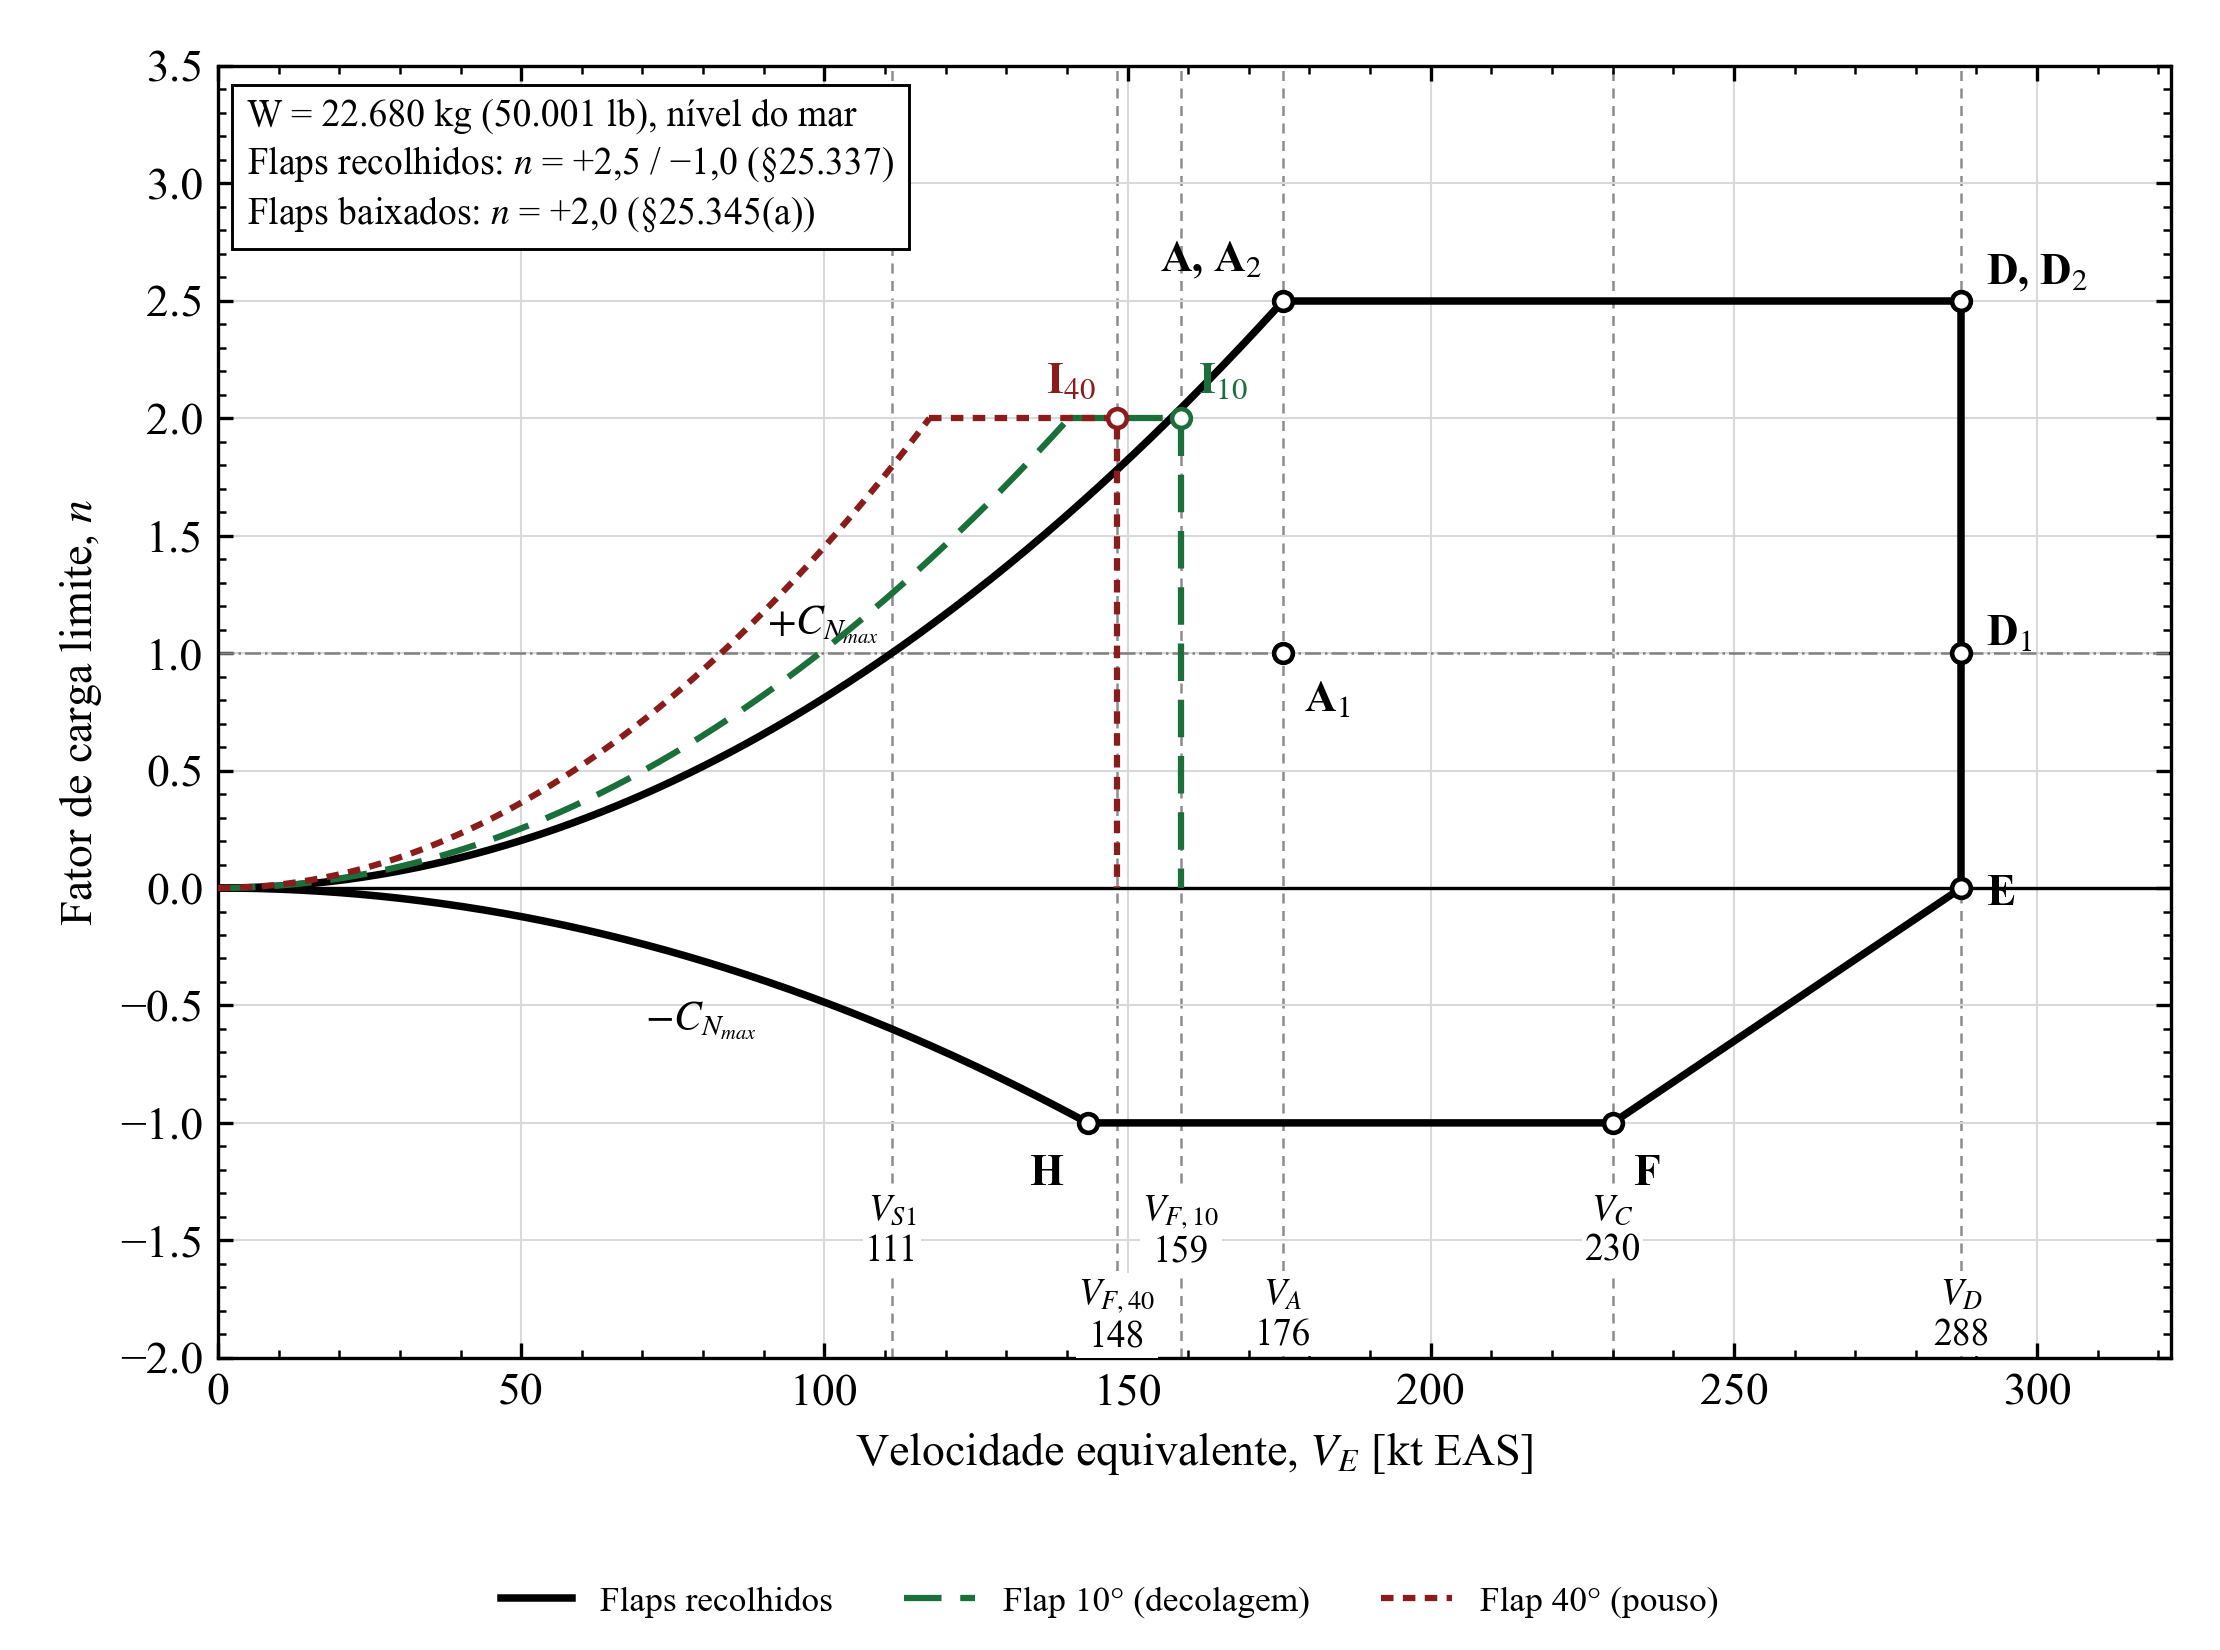
\includegraphics[width=0.95\linewidth]{images/cargas/vn_manobra_sl.png}
    \caption{Diagrama V-n de manobra com flaps recolhidos e baixados (10° e 40°), MTOW, nível do mar.}
    \label{fig:vn_manobra}
\end{figure}

\begin{figure}[H]
    \centering
    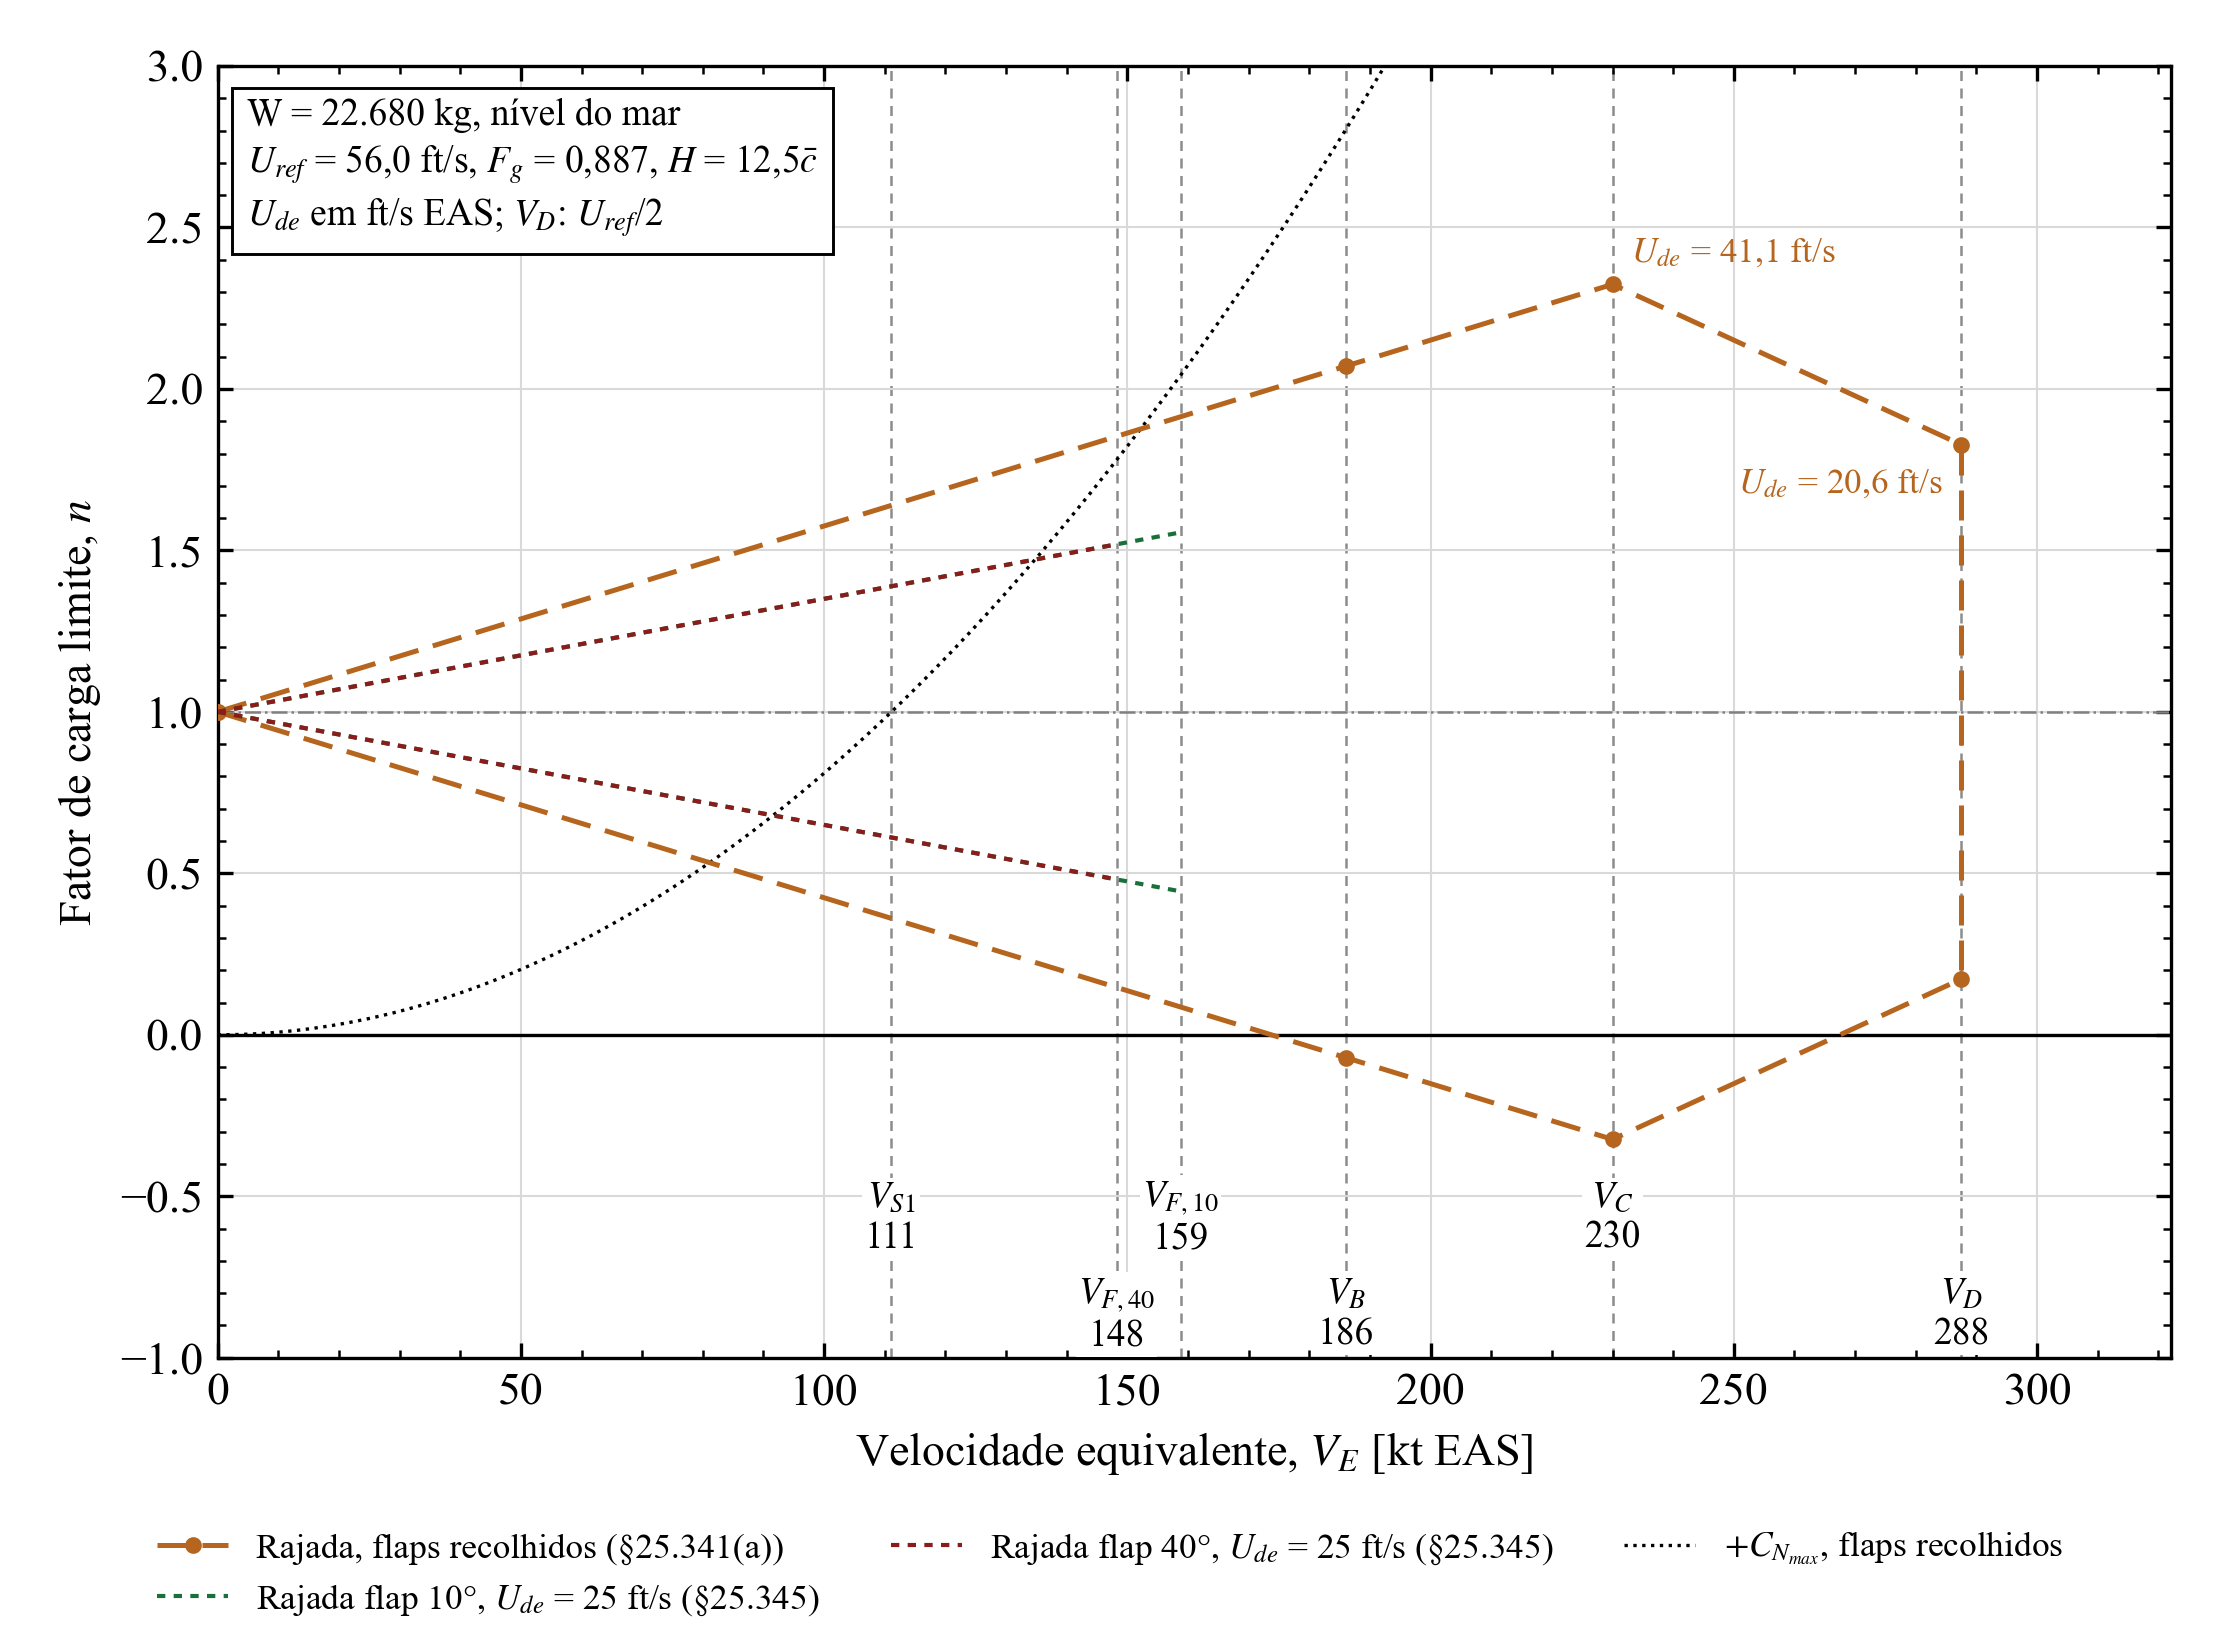
\includegraphics[width=0.95\linewidth]{images/cargas/vn_rajada_sl.png}
    \caption{Diagrama V-n de rajada com flaps recolhidos e baixados (10° e 40°), MTOW, nível do mar.}
    \label{fig:vn_rajada}
\end{figure}

\begin{figure}[H]
    \centering
    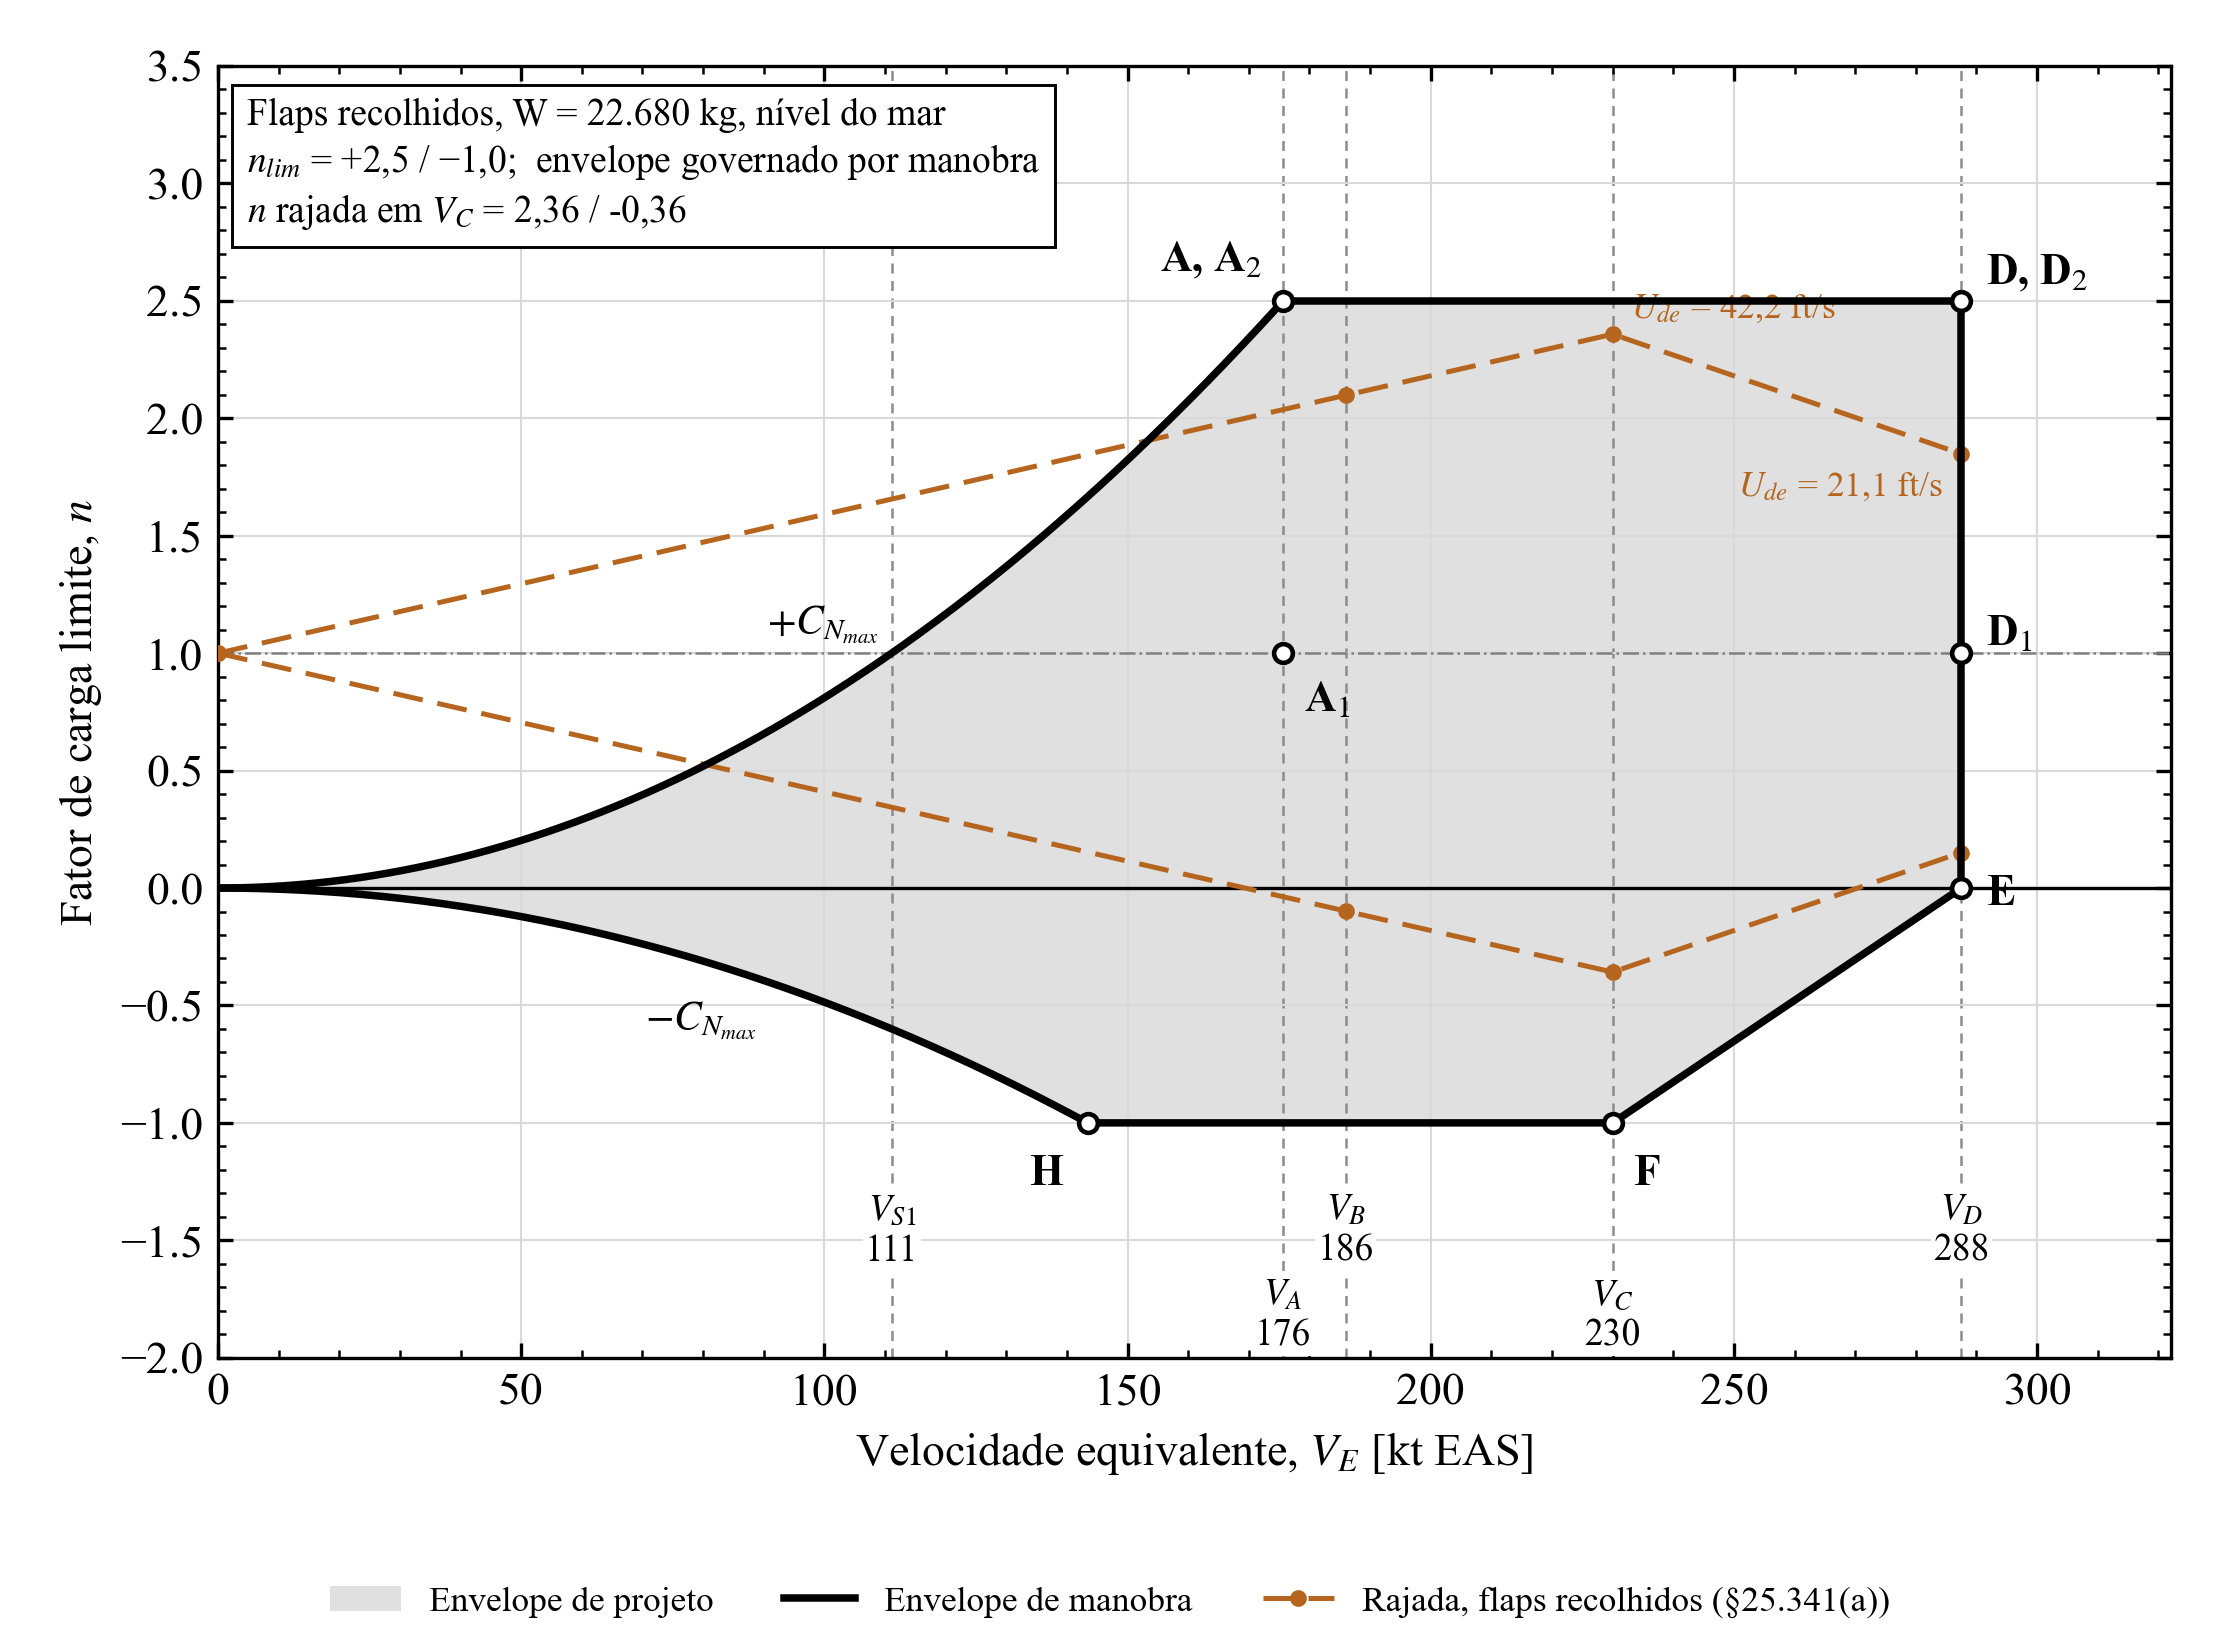
\includegraphics[width=0.95\linewidth]{images/cargas/vn_projeto.png}
    \caption{Envelope de projeto (manobra e rajada) com flaps recolhidos, MTOW, nível do mar.}
    \label{fig:vn_projeto_sl}
\end{figure}

\begin{figure}[H]
    \centering
    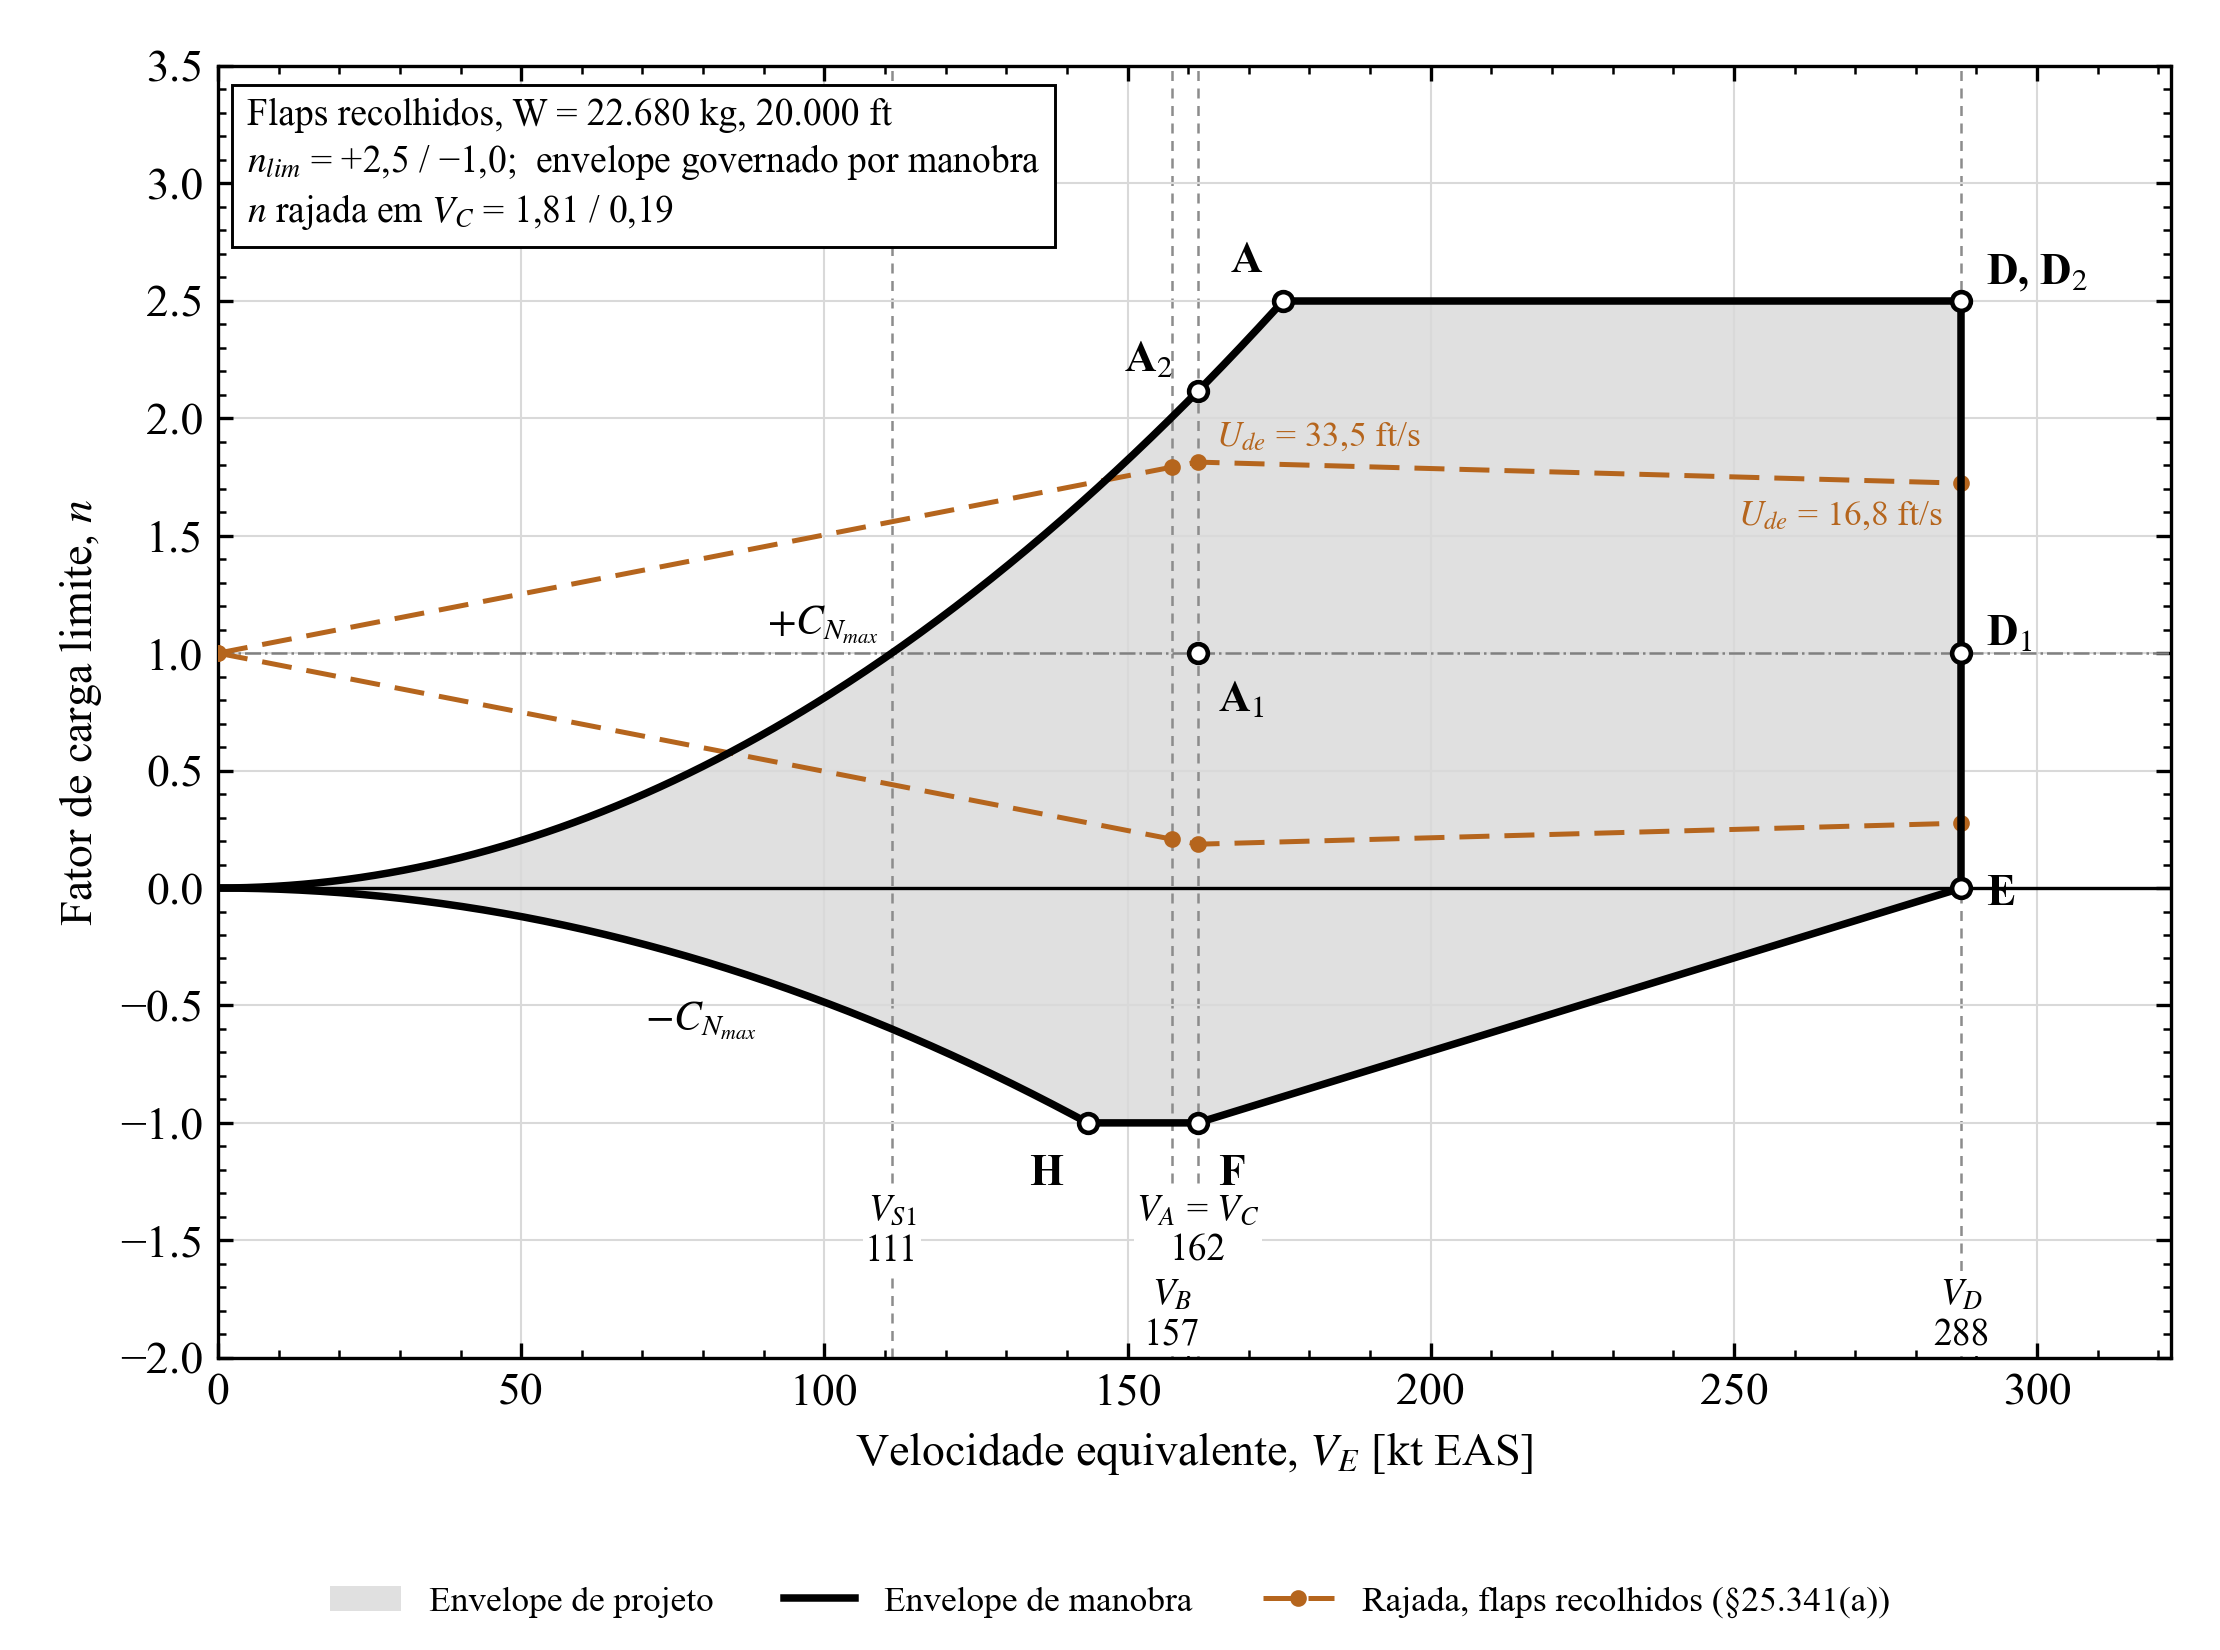
\includegraphics[width=0.95\linewidth]{images/cargas/vn_projeto_20000ft.png}
    \caption{Envelope de projeto (manobra e rajada) com flaps recolhidos, MTOW, 20.000 ft.}
    \label{fig:vn_projeto_20k}
\end{figure}




\section{Cargas na Asa}
\label{sec:cargas_asa}

A análise de cargas na asa considerou as condições de manobra e os pontos do envelope de rajada. As cargas aerodinâmicas foram determinadas para cada condição e distribuídas ao longo da envergadura pelo método de Stender, permitindo o cálculo dos esforços internos correspondentes.

\subsection*{Manobra e Balanceamento Longitudinal}

Para as condições simétricas de manobra, a sustentação da asa foi determinada a partir do equilíbrio longitudinal da aeronave, considerando as forças aerodinâmicas da asa e da EH, o peso e o momento aerodinâmico do conjunto asa--fuselagem, conforme representado na \autoref{fig:cargas_dcl_balanceamento}. Dessa forma, a carga de balanceamento da EH foi considerada na determinação dos carregamentos da asa, conforme o \S~25.331 do 14 CFR Part 25. Os momentos produzidos pelas forças de arrasto e tração foram desconsiderados no equilíbrio longitudinal.

\begin{figure}[H]
    \centering
    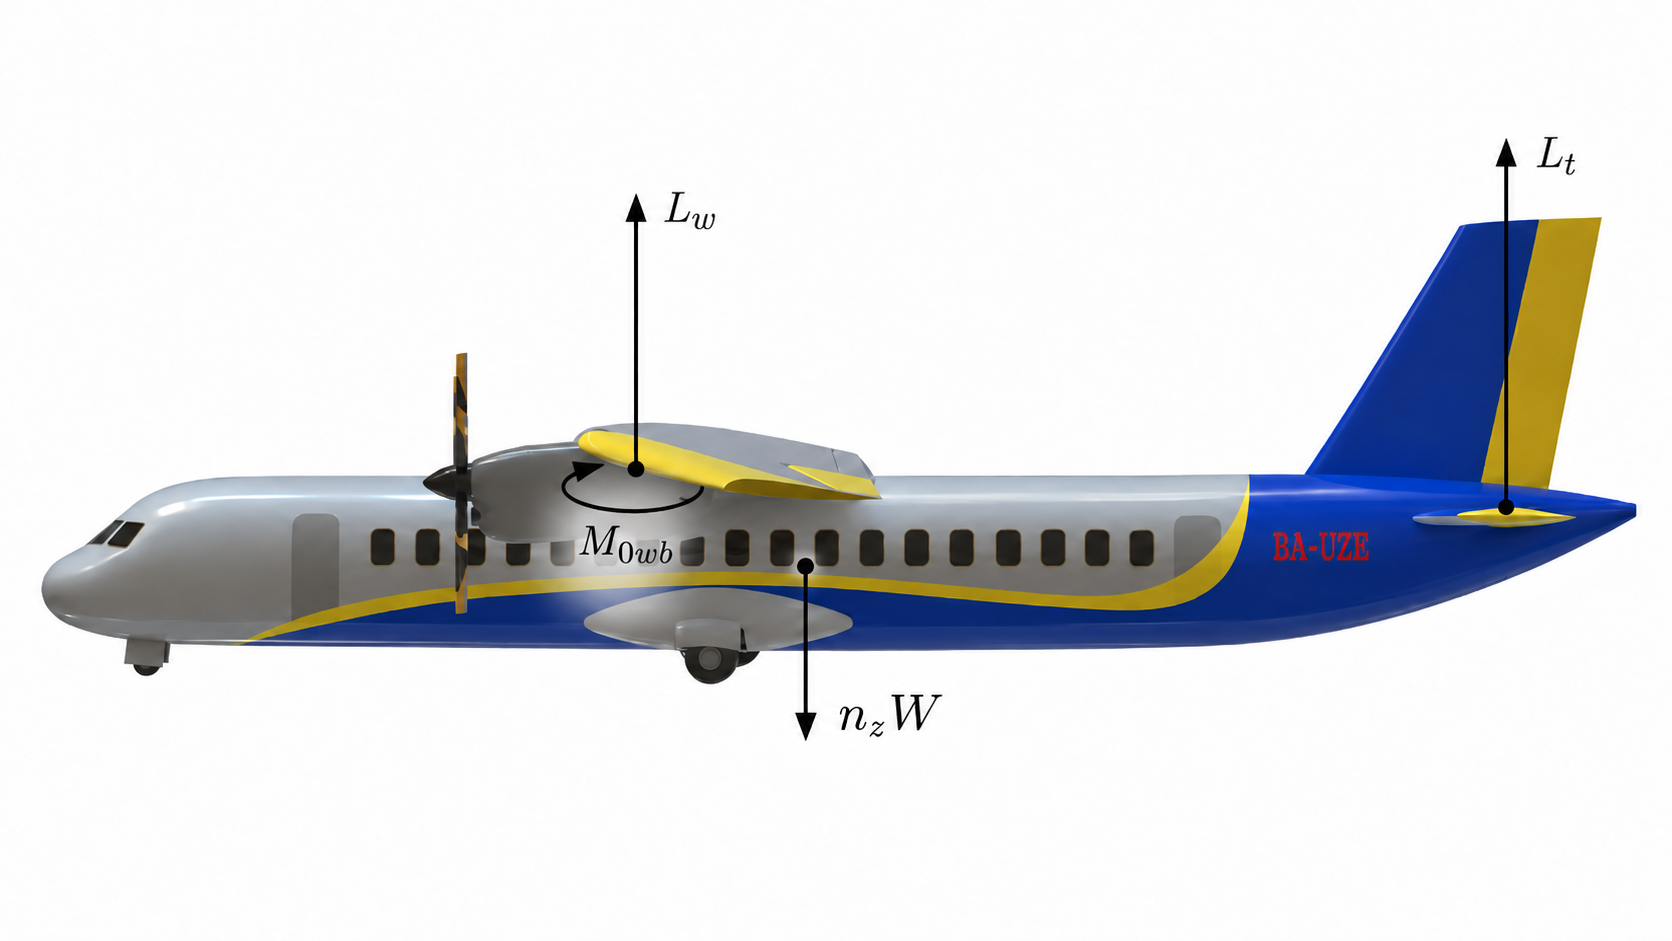
\includegraphics[width=0.85\linewidth]{images/cargas/DCL_cargas.png}
    \caption{Diagrama de corpo livre do equilíbrio longitudinal.}
    \label{fig:cargas_dcl_balanceamento}
\end{figure}

A carga resultante na asa foi calculada por:
\begin{equation}
    L_w=-\frac{\rho_0 S_w\bar{c}C_{M_0}}{2\bar{l}_t}V_{\mathrm{EAS}}^2
    +\frac{W\left[\bar{l}_t-(h_{CG}-h_0)\bar{c}\right]}{\bar{l}_t}\,n_z,
    \label{eq:cargas_Lw}
\end{equation}

A Equação~\ref{eq:cargas_Lw} foi avaliada para as combinações de velocidade, fator de carga e posição do CG consideradas nos diagramas $V$--$n$.

\subsection*{Rajada}

Para os pontos do envelope de rajada, os fatores de carga obtidos conforme a metodologia adotada com referência ao \S~25.341 do 14 CFR Part 25 foram aplicados à Equação~\ref{eq:cargas_Lw}.

\subsection*{Arrasto, Momento Aerodinâmico e Distribuição}

O arrasto de perfil foi estimado a partir da sustentação local, obtida pela distribuição de Stender, e das polares bidimensionais dos perfis utilizados. Os coeficientes de momento aerodinâmico também foram obtidos dessas polares e considerados constantes para cada perfil, com o momento referido a $25\%$ da corda local.

Para as regiões da asa encobertas pela fuselagem, as parcelas de sustentação, arrasto e momento aerodinâmico foram redistribuídas sobre os trechos expostos, preservando-se as resultantes dos carregamentos.

As componentes de força foram calculadas pela transformação dos eixos aerodinâmicos para os eixos da aeronave:
\begin{align}
    F_z &= L_w\cos\alpha+D_w\sin\alpha, \\
    F_x &=-L_w\sin\alpha+D_w\cos\alpha.
    \label{eq:cargas_transform_asa}
\end{align}

\subsection*{Resultados}

Os carregamentos distribuídos obtidos pelo método de Stender são apresentados na \autoref{fig:cargas_asa_fz}, na \autoref{fig:cargas_asa_fx} e na \autoref{fig:cargas_asa_ma}.

%% Os gráficos de distribuição abaixo abrangem TODAS as condições de carga da asa.
\begin{figure}[H]
    \centering
    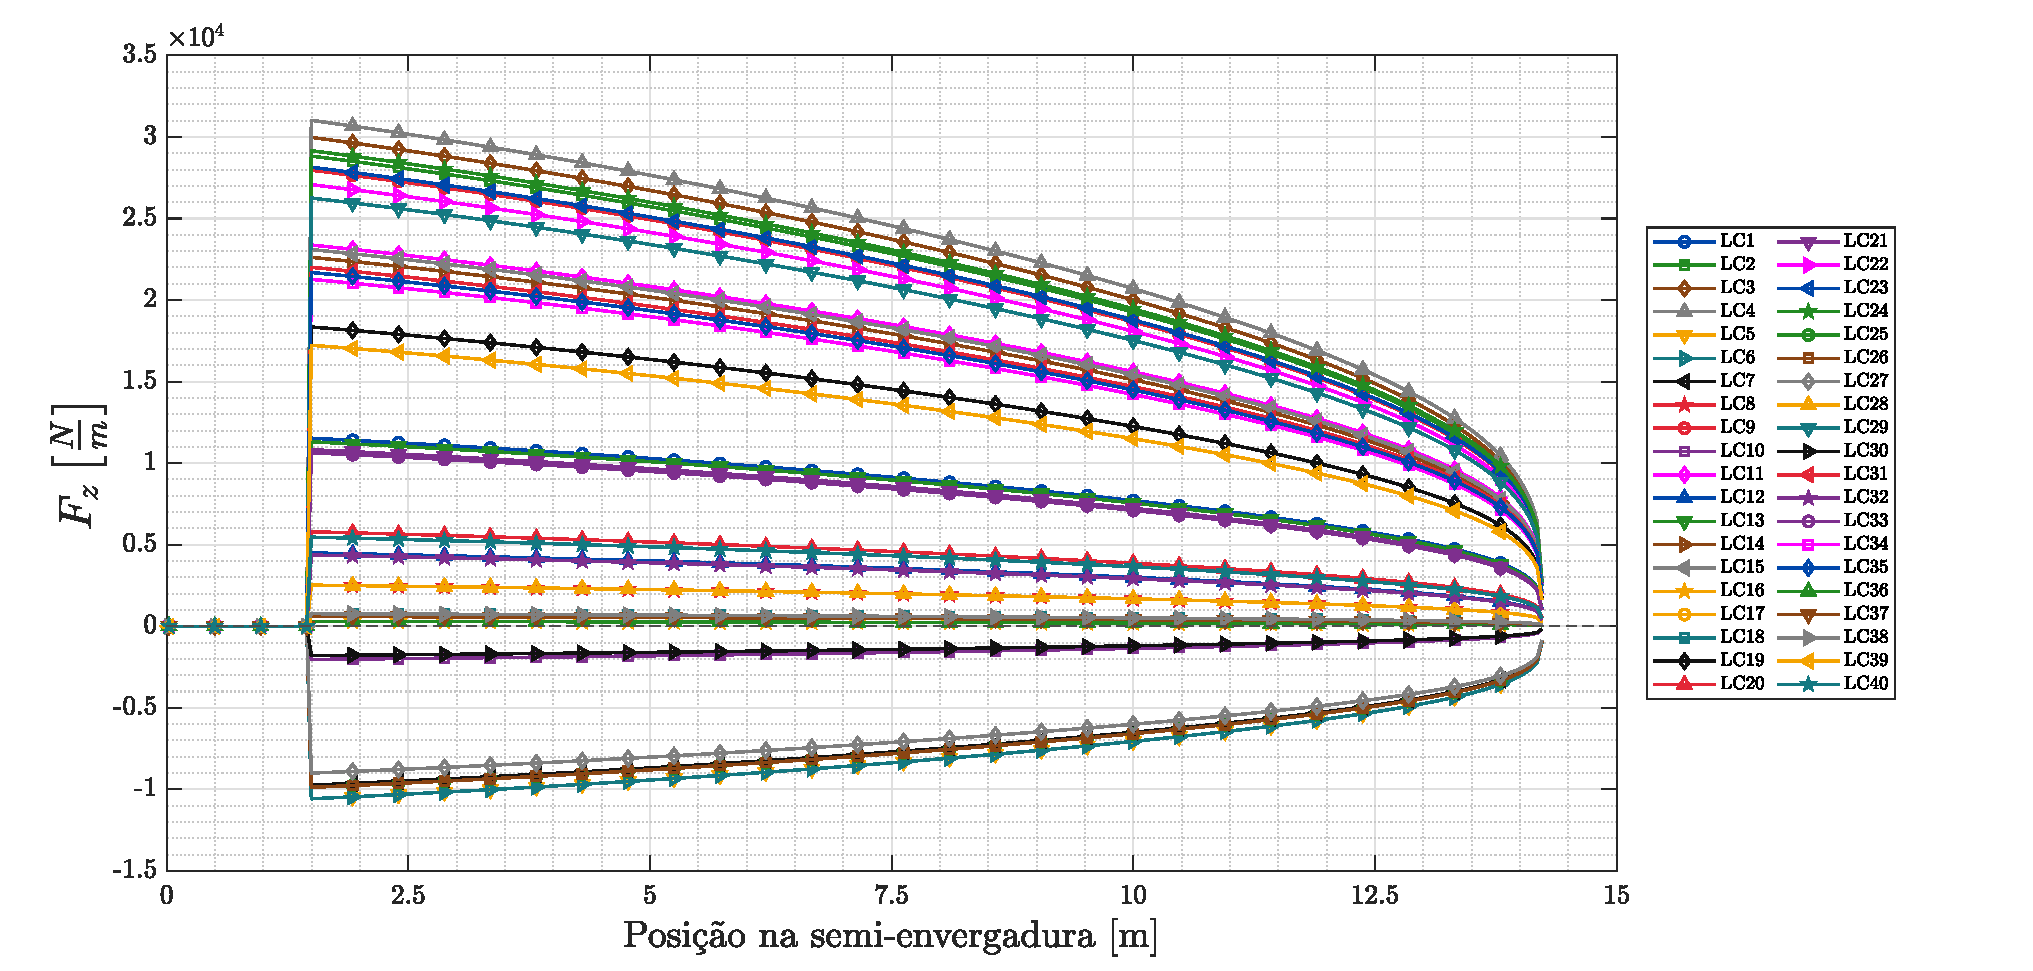
\includegraphics[width=1\linewidth]{images/cargas/wing_Fz.eps}
    \caption{$F_z$ distribuído na asa.}
    \label{fig:cargas_asa_fz}
\end{figure}

\begin{figure}[H]
    \centering
    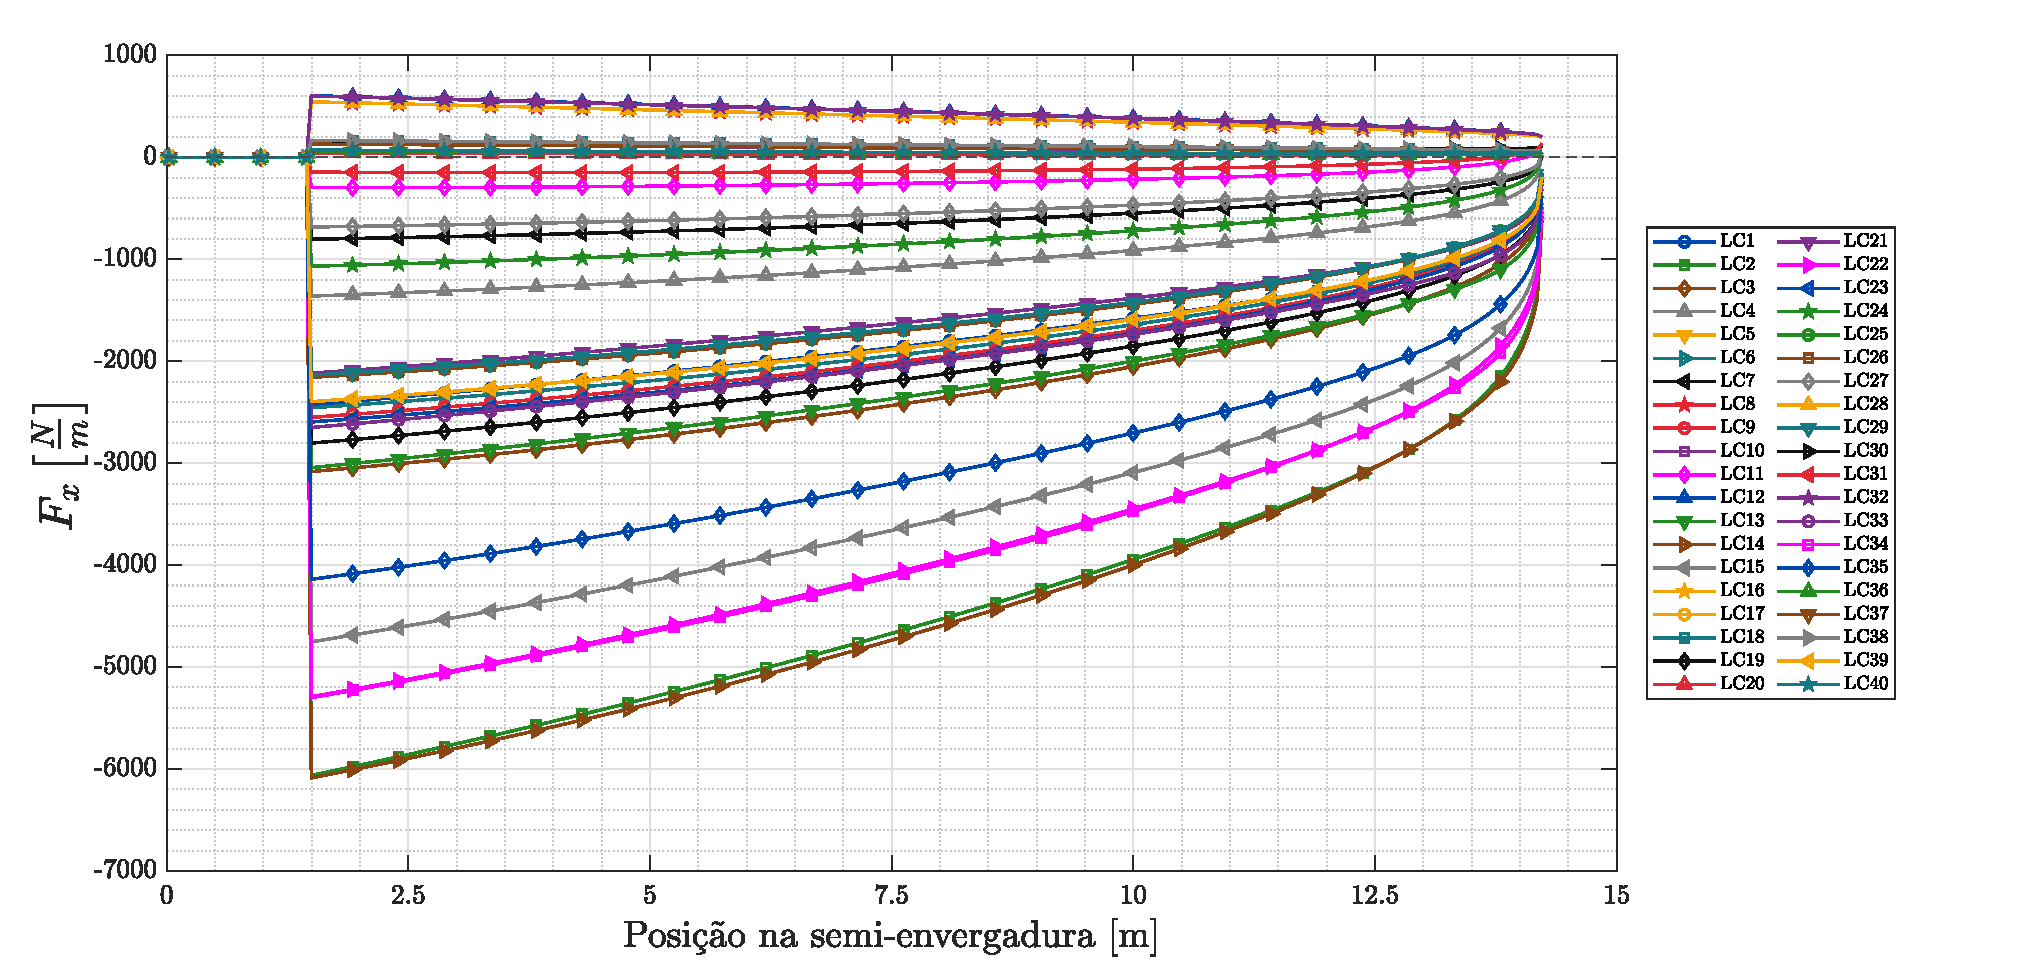
\includegraphics[width=1\linewidth]{images/cargas/wing_Fx.eps}
    \caption{$F_x$ distribuído na asa.}
    \label{fig:cargas_asa_fx}
\end{figure}

\begin{figure}[H]
    \centering
    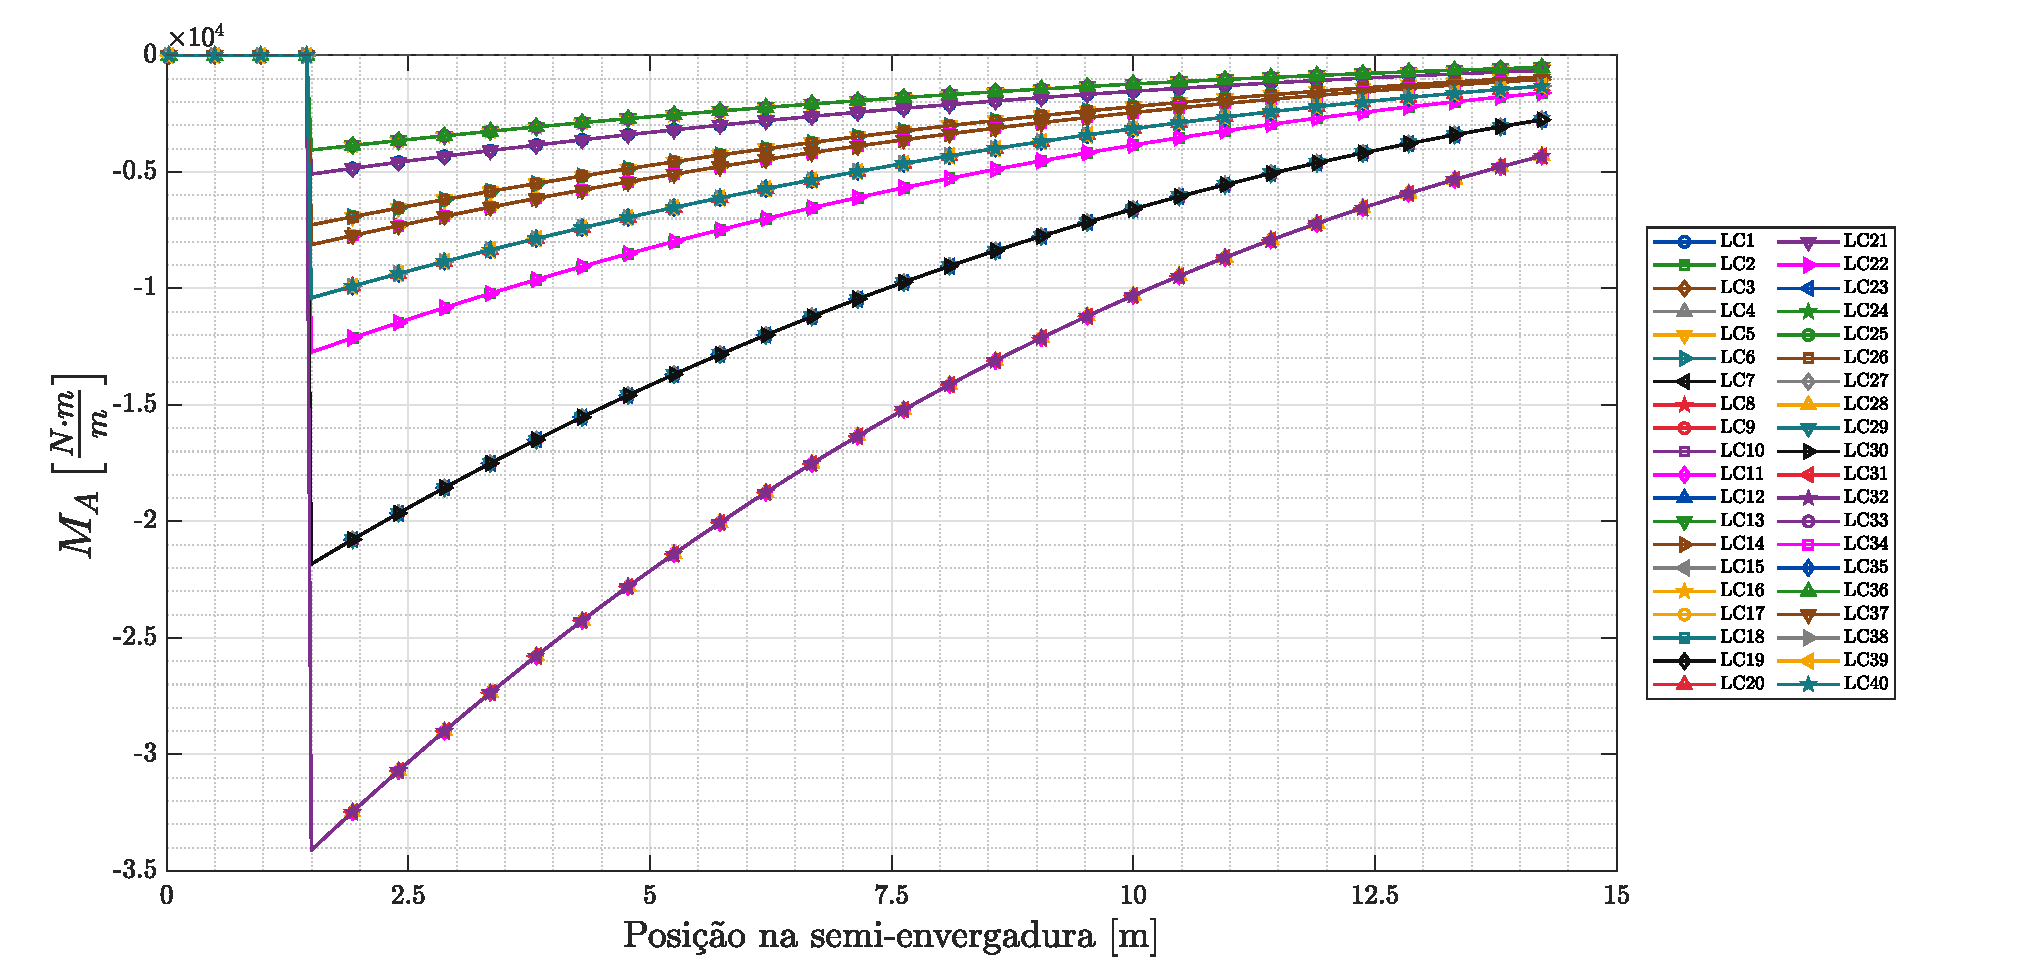
\includegraphics[width=1\linewidth]{images/cargas/wing_MA.eps}
    \caption{$MA$ distribuído na asa.}
    \label{fig:cargas_asa_ma}
\end{figure}

As condições de voo correspondentes aos casos críticos identificados para a asa são resumidas na Tabela~\ref{tab:cargas_criticas_asa}.

\begin{table}[H]
    \centering
    \caption{Condições críticas da asa.}
    \label{tab:cargas_criticas_asa}
    \vspace{1mm}
    \begingroup
    \footnotesize
    \setlength{\tabcolsep}{5pt}
    \renewcommand{\arraystretch}{1.35}
    \begin{tabular}{@{}lccccccc@{}}
        \noalign{\hrule height 0.8pt}
        \textbf{N\textsuperscript{o}} & \textbf{Tipo} & \textbf{14 CFR Part 25} & \textbf{TOW} & \textbf{CG} & \textbf{Flap} & \textbf{Velocidade} & \boldmath$n_z$\\
        \hline
        LC4  & Manobra & \S~25.331 & MTOW & Dianteiro & Recolhido & $V_D$ & $2{,}50$\\
        LC5  & Manobra & \S~25.337 & MTOW & Dianteiro & Recolhido & $V_{S,\mathrm{neg}}$ & $-1{,}00$\\
        LC12 & Rajada  & \S~25.341 & MTOW & Dianteiro & Recolhido & $V_D$ & $0{,}173$\\
        LC14 & Manobra & \S~25.345 & MTOW & Dianteiro & Estendido & $V_A$ & $2{,}00$\\
        LC16 & Manobra & \S~25.345 & MTOW & Dianteiro & Estendido & $V_{SF}$ & $0{,}00$\\
        \noalign{\hrule height 0.8pt}
    \end{tabular}
    \endgroup
\end{table}

Os esforços internos correspondentes às condições críticas são apresentados na \autoref{fig:cargas_asa_crit_fz}, na \autoref{fig:cargas_asa_crit_fx} e na \autoref{fig:cargas_asa_crit_my}.

%% Os gráficos de esforços abaixo incluem SOMENTE as condições críticas.
\begin{figure}[H]
    \centering
    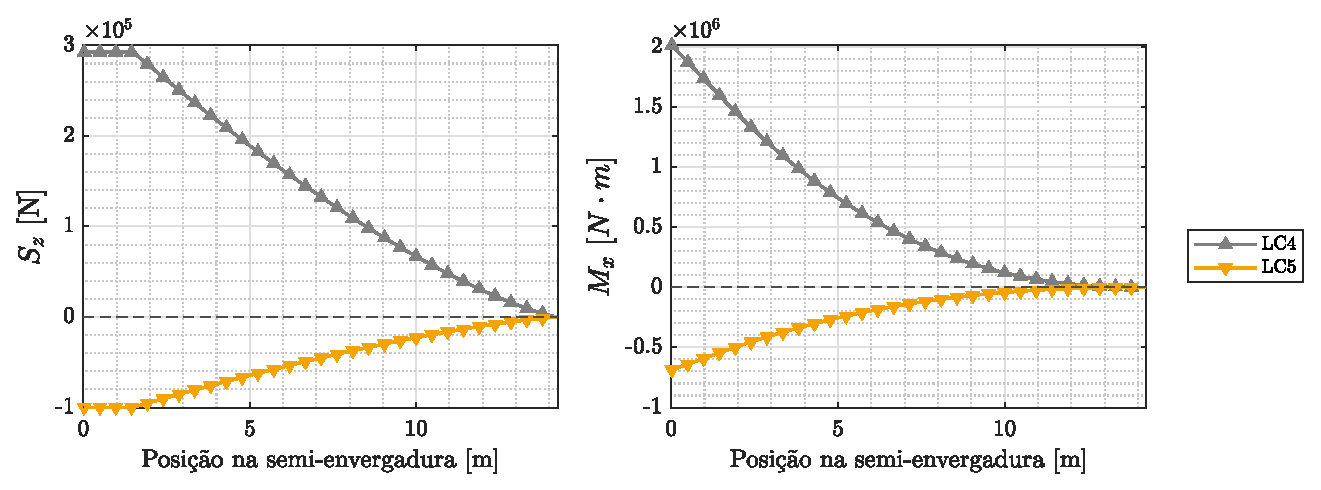
\includegraphics[width=0.91\linewidth]{images/cargas/esforcos_Fz_asa.eps}
    \caption{Esforços críticos associados a $F_z$ na asa.}
    \label{fig:cargas_asa_crit_fz}
\end{figure}

\begin{figure}[H]
    \centering
    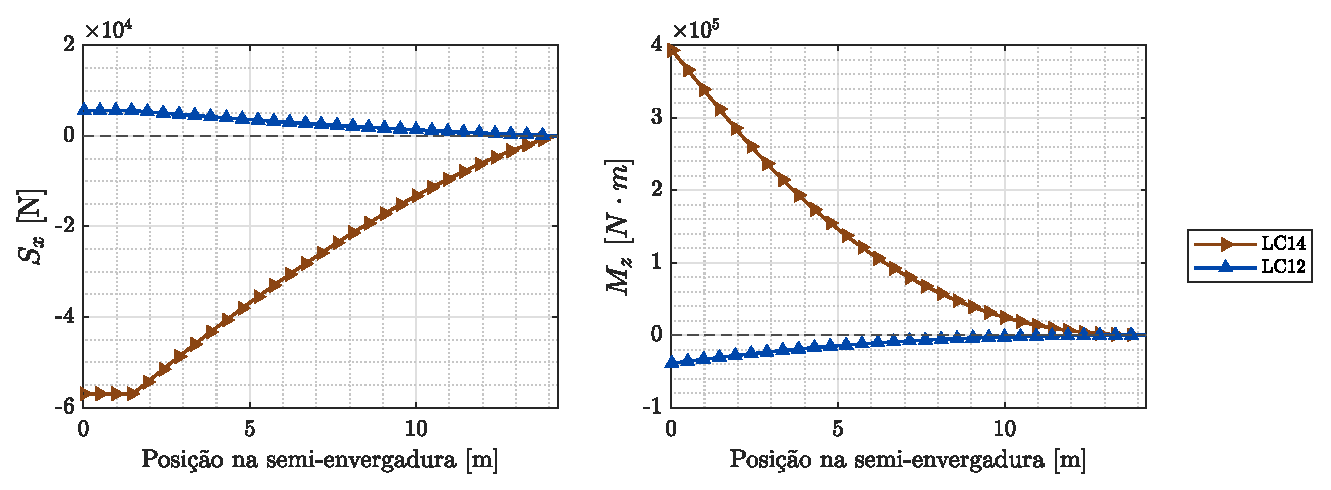
\includegraphics[width=0.91\linewidth]{images/cargas/esforcos_Fx_asa.eps}
    \caption{Esforços críticos associados a $F_x$ na asa.}
    \label{fig:cargas_asa_crit_fx}
\end{figure}

\begin{figure}[H]
    \centering
    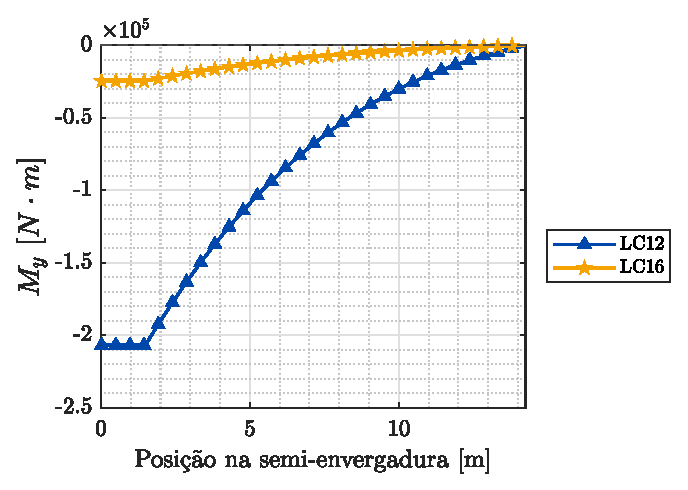
\includegraphics[width=0.55\linewidth]{images/cargas/esforco_MA_asa.eps}
    \caption{Momento torsor crítico $M_y$ na asa.}
    \label{fig:cargas_asa_crit_my}
\end{figure}

\section{Cargas na EH}
\label{sec:cargas_eh}

A análise de cargas da EH considerou as condições de balanceamento, manobra e rajada. Para cada condição, a força aerodinâmica foi determinada e distribuída ao longo da envergadura pelo método de Stender, permitindo o cálculo dos esforços internos correspondentes.

\subsection*{Balanceamento}

As cargas de balanceamento da EH foram determinadas pelo equilíbrio longitudinal apresentado na \autoref{fig:cargas_dcl_balanceamento}, de acordo com
\begin{equation}
    L_t=\frac{\rho_0S_w\bar{c}C_{M_0}}{2\bar{l}_t}V_{\mathrm{EAS}}^2
    +\frac{W(h_{CG}-h_0)\bar{c}}{\bar{l}_t}\,n_z.
    \label{eq:cargas_Lt}
\end{equation}

A Equação~\ref{eq:cargas_Lt} foi aplicada às combinações de velocidade, fator de carga e CG consideradas no envelope.

\subsection*{Manobras}

As cargas de manobra foram estimadas com referência ao \S~25.331 do 14 CFR Part 25. A manobra não corrigida considerou as deflexões máximas positiva e negativa do profundor em $V_A$. Para a manobra corrigida, incluiu-se de forma aproximada o efeito da aceleração angular de arfagem e do momento de inércia longitudinal, como avaliação preliminar do requisito.

\subsection*{Rajada}

As cargas de rajada foram calculadas com referência ao \S~25.341 do 14 CFR Part 25, somando-se à carga de balanceamento em voo a $1\,g$ o incremento aerodinâmico provocado pela rajada:
\begin{equation}
    L_{t,\mathrm{raj}}=L_{t,\mathrm{bal},\,1g}\pm\Delta L_{t,g},
    \label{eq:cargas_Lt_raj}
\end{equation}
\begin{equation}
    \Delta L_{t,g}=\frac{1}{2}\rho_0V_{\mathrm{EAS}}S_ta_tU_gK_g
    \left(1-\frac{\mathrm{d}\varepsilon}{\mathrm{d}\alpha}\right).
    \label{eq:cargas_dLt_raj}
\end{equation}

\subsection*{Arrasto, Momento Aerodinâmico e Distribuição}

De modo semelhante à asa, o arrasto da EH foi estimado com base na sustentação local e nas polares bidimensionais dos perfis utilizados. O momento aerodinâmico foi calculado em relação a $25\%$ da corda local, utilizando as distribuições de carregamento das Figuras B6, B7 e B8 do Apêndice B da CS-VLA, conforme a condição analisada. Essa abordagem, já empregada na metodologia de cargas adotada, foi utilizada como estimativa preliminar, embora a aeronave deste projeto pertença à categoria Transporte.

Os carregamentos das regiões encobertas pela EV foram redistribuídos entre os trechos expostos da EH, preservando-se os valores totais das resultantes. As componentes $F_z$ e $F_x$ foram obtidas pela transformação das forças aerodinâmicas para os eixos da aeronave.

\subsection*{Resultados}

Os carregamentos distribuídos obtidos pelo método de Stender são apresentados na \autoref{fig:cargas_eh_fz}, na \autoref{fig:cargas_eh_fx} e na \autoref{fig:cargas_eh_ma}.

%% Os gráficos de distribuição abaixo abrangem TODAS as condições de carga da EH.
\begin{figure}[H]
    \centering
    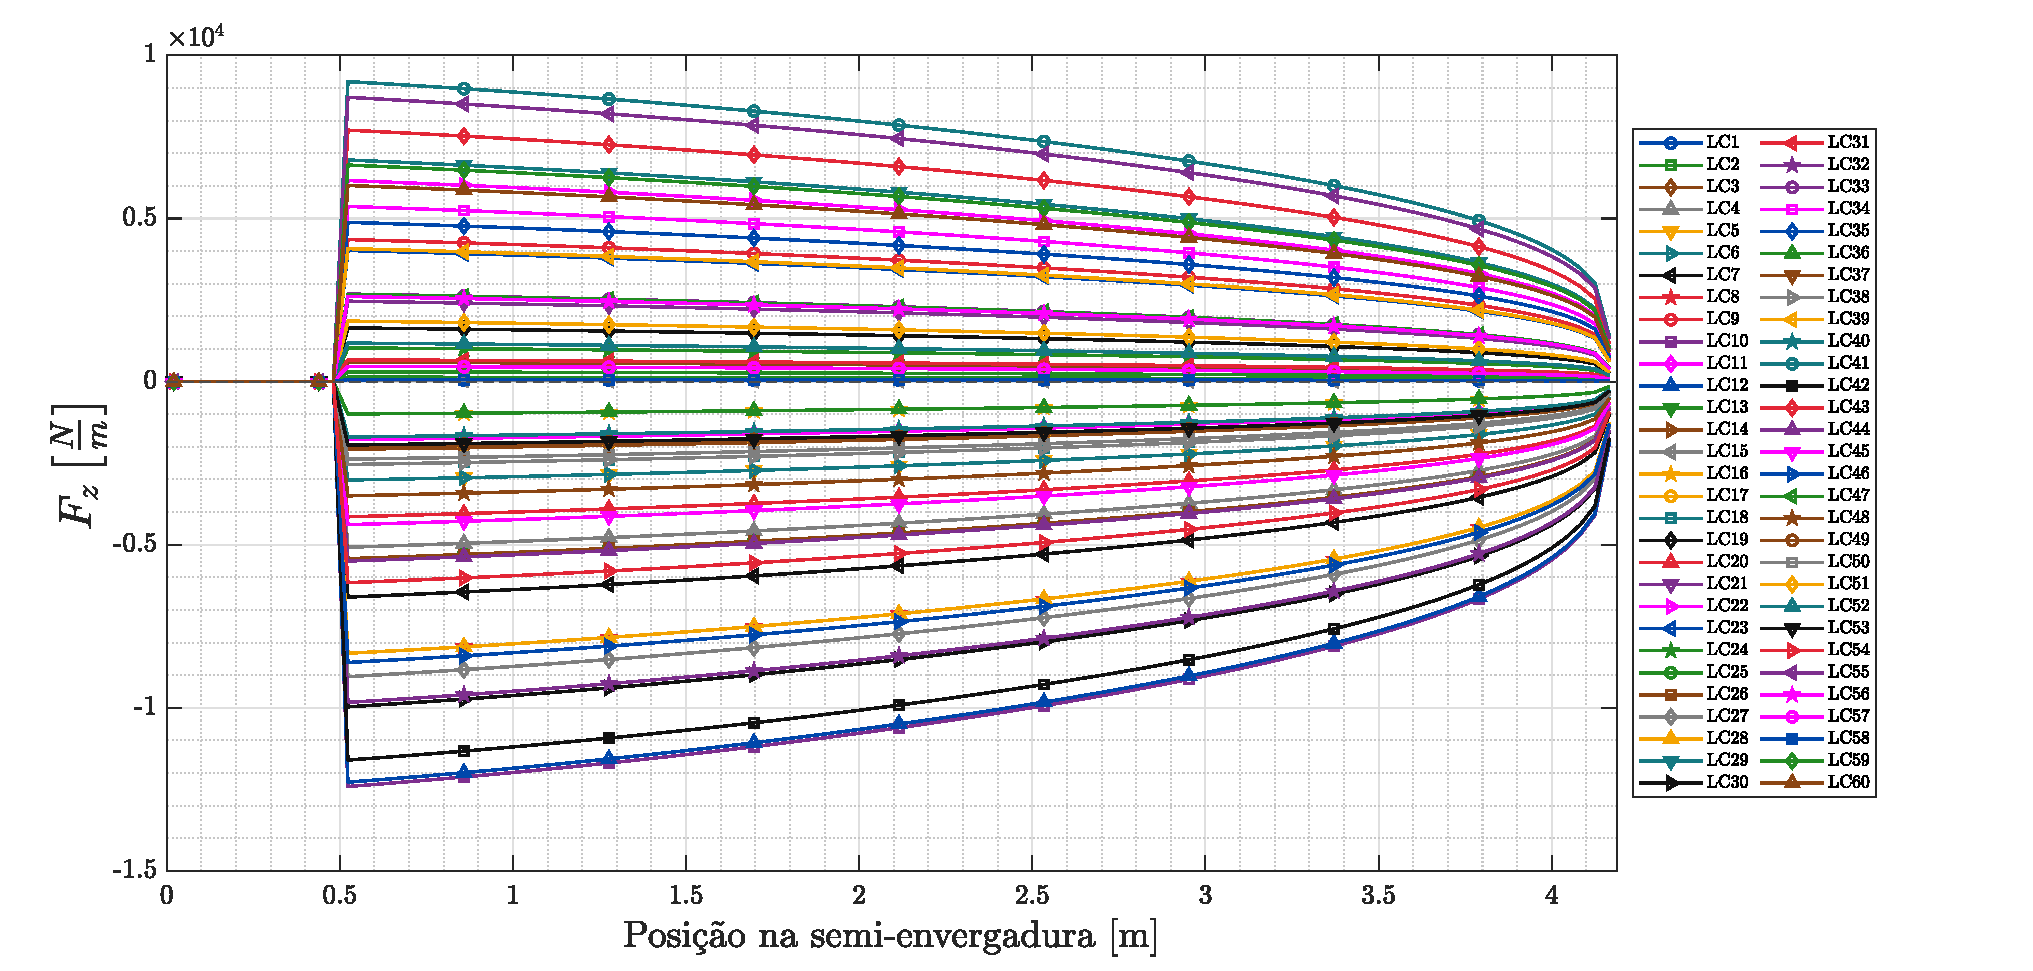
\includegraphics[width=1\linewidth]{images/cargas/htail_Fz.eps}
    \caption{$F_z$ distribuído na EH.}
    \label{fig:cargas_eh_fz}
\end{figure}

\begin{figure}[H]
    \centering
    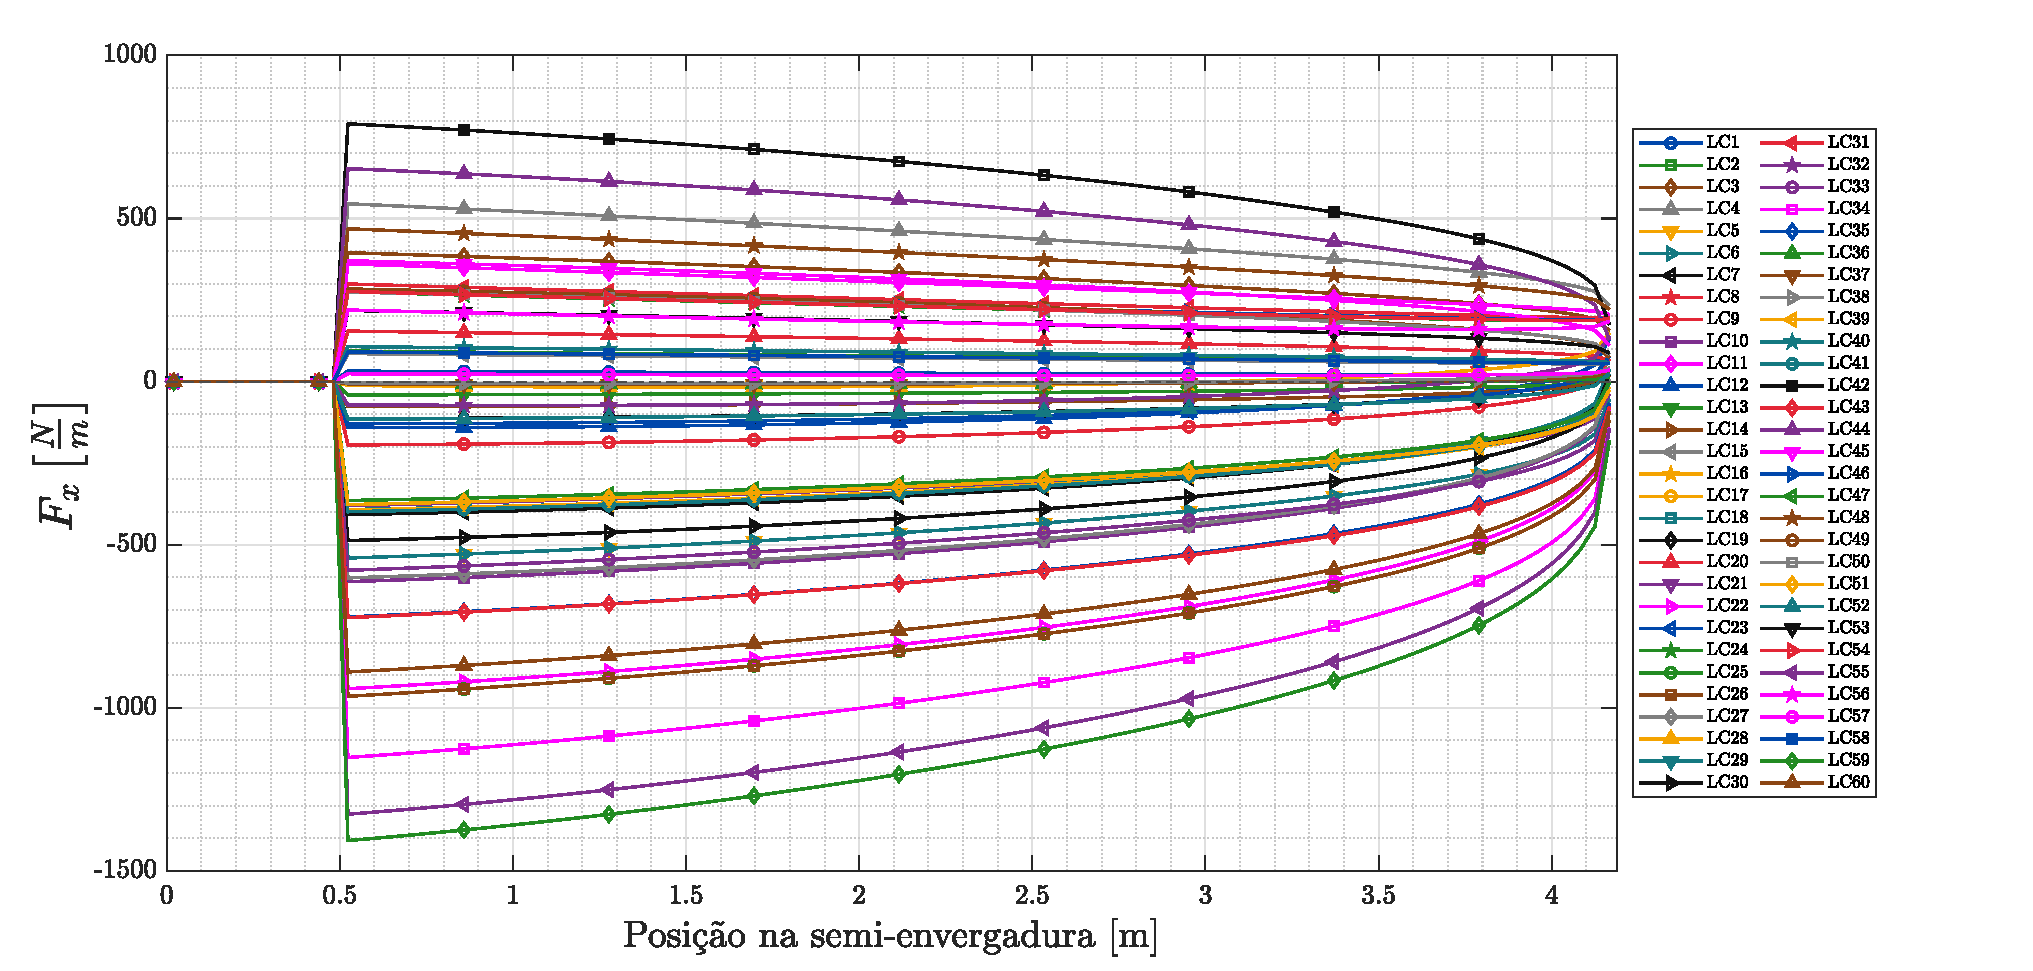
\includegraphics[width=1\linewidth]{images/cargas/htail_Fx.eps}
    \caption{$F_x$ distribuído na EH.}
    \label{fig:cargas_eh_fx}
\end{figure}

\begin{figure}[H]
    \centering
    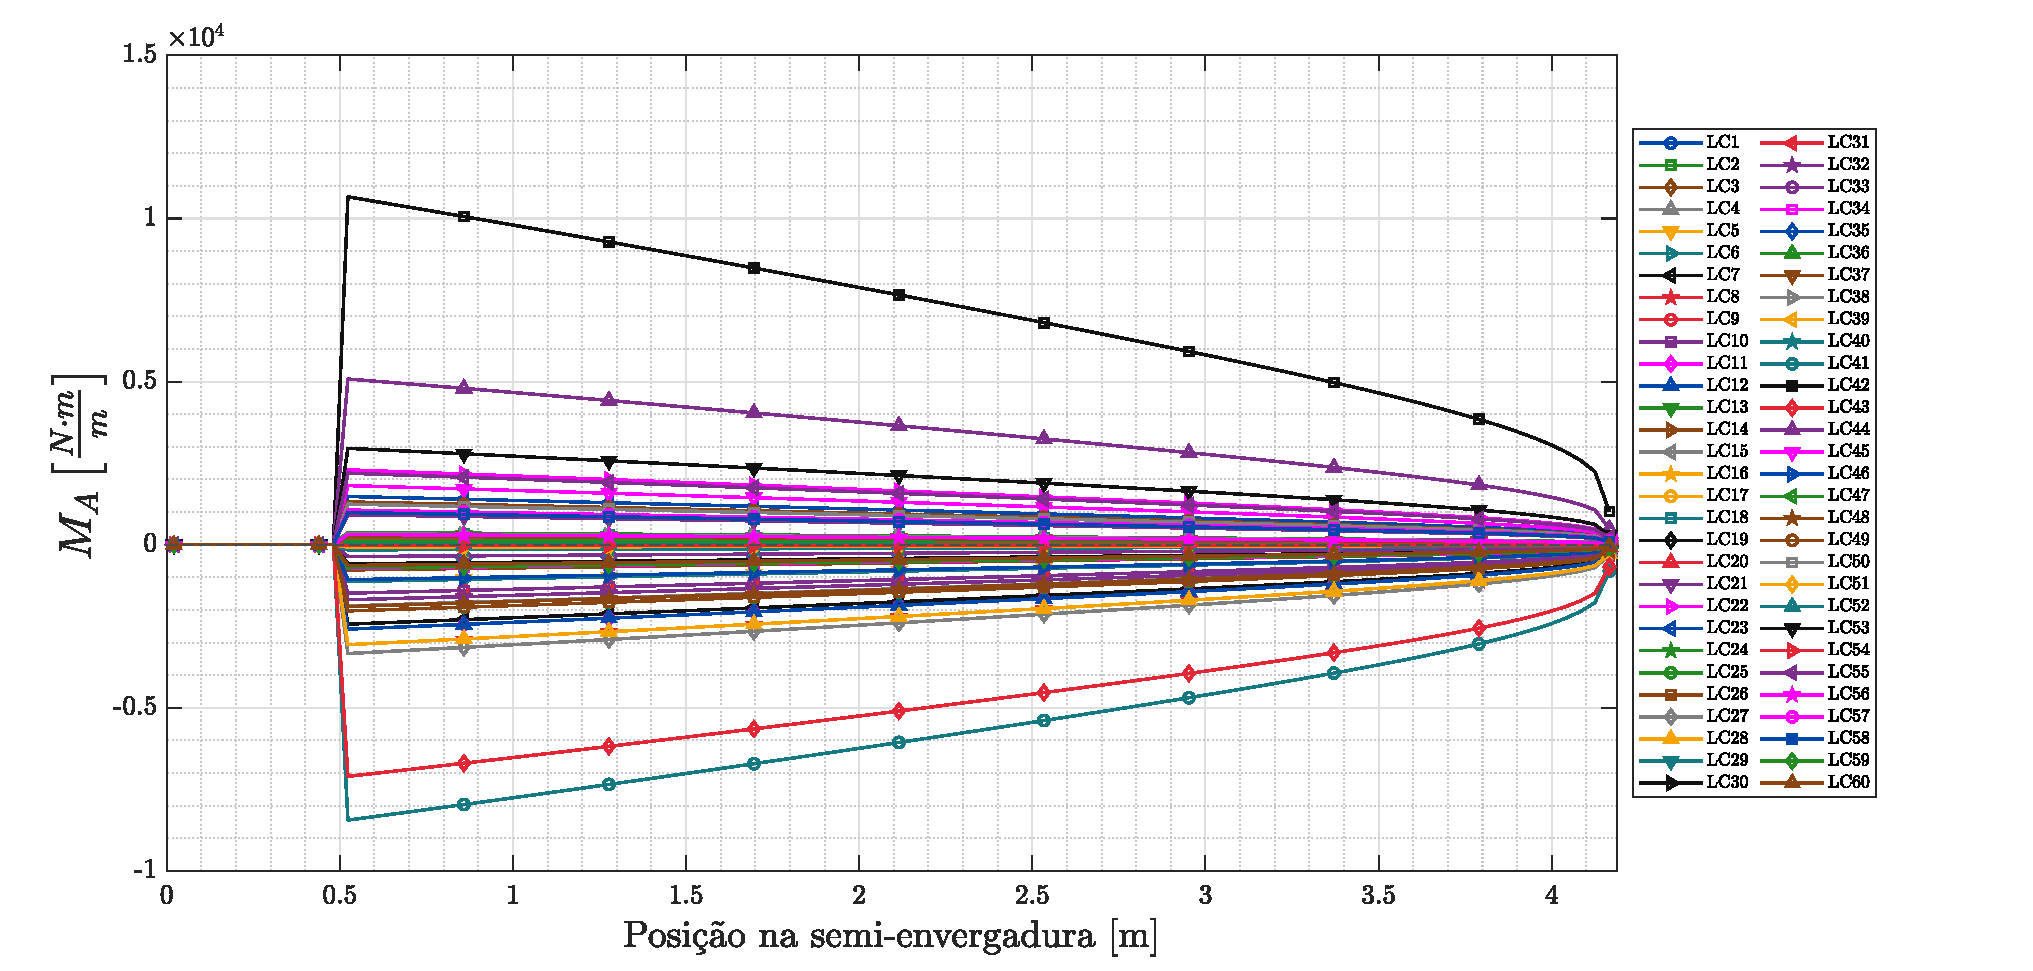
\includegraphics[width=1\linewidth]{images/cargas/htail_MA.eps}
    \caption{$MA$ distribuído na EH.}
    \label{fig:cargas_eh_ma}
\end{figure}

As condições de voo correspondentes aos casos críticos identificados para a EH são resumidas na Tabela~\ref{tab:cargas_criticas_eh}.

\begin{table}[H]
    \centering
    \caption{Condições críticas da EH.}
    \label{tab:cargas_criticas_eh}
    \vspace{1mm}
    \begingroup
    \footnotesize
    \setlength{\tabcolsep}{5pt}
    \renewcommand{\arraystretch}{1.35}
    \begin{tabular}{@{}lccccccc@{}}
        \noalign{\hrule height 0.8pt}
        \textbf{N\textsuperscript{o}} & \textbf{Tipo} & \textbf{14 CFR Part 25} & \textbf{TOW} & \textbf{CG} & \textbf{Flap} & \textbf{Velocidade} & \boldmath$n_z$\\
        \hline
        LC10 & Rajada & \S~25.341 & MTOW & Dianteiro & Recolhido & $V_C$ & $-0{,}32$\\
        LC41 & \shortstack{Manobra não\\corrigida (+)} & \S~25.331 & MTOW & --- & Recolhido & $V_A$ & $1{,}00$\\
        LC42 & \shortstack{Manobra não\\corrigida ($-$)} & \S~25.331 & MTOW & --- & Recolhido & $V_A$ & $1{,}00$\\
        LC59 & \shortstack{Manobra corrigida\\(picada)} & \S~25.331 & MTOW & Traseiro & Estendido & $V_A$ & $2{,}00$\\
        \noalign{\hrule height 0.8pt}
    \end{tabular}
    \endgroup
\end{table}

Os esforços internos correspondentes às condições críticas são apresentados na \autoref{fig:cargas_eh_crit_fz}, na \autoref{fig:cargas_eh_crit_fx} e na \autoref{fig:cargas_eh_crit_my}.

\begin{figure}[H]
    \centering
    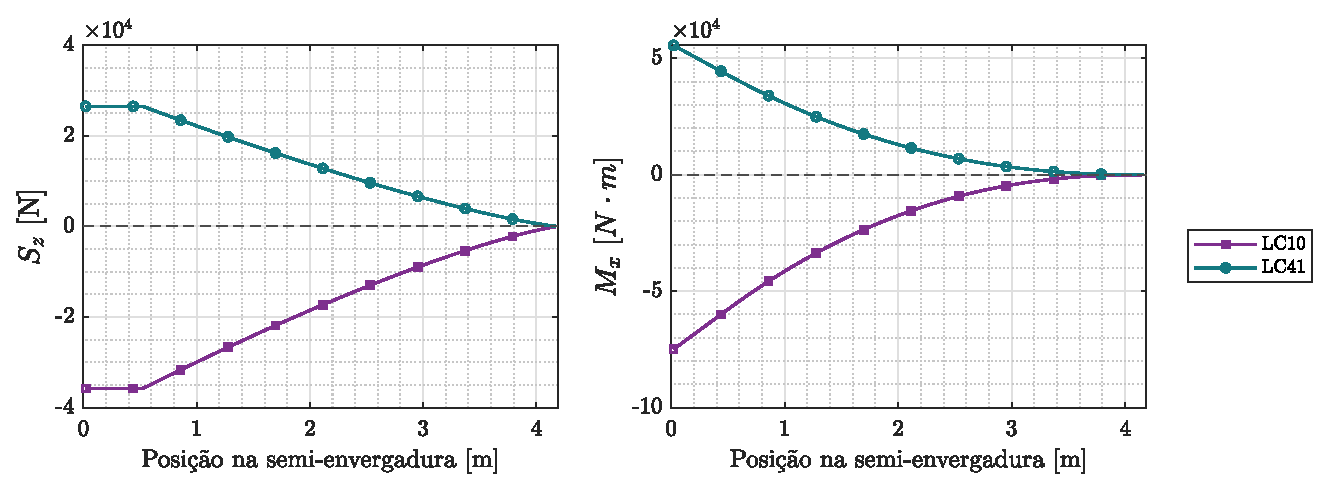
\includegraphics[width=0.91\linewidth]{images/cargas/esforcos_Fz_eh.eps}
    \caption{Esforços críticos associados a $F_z$ na EH.}
    \label{fig:cargas_eh_crit_fz}
\end{figure}

\begin{figure}[H]
    \centering
    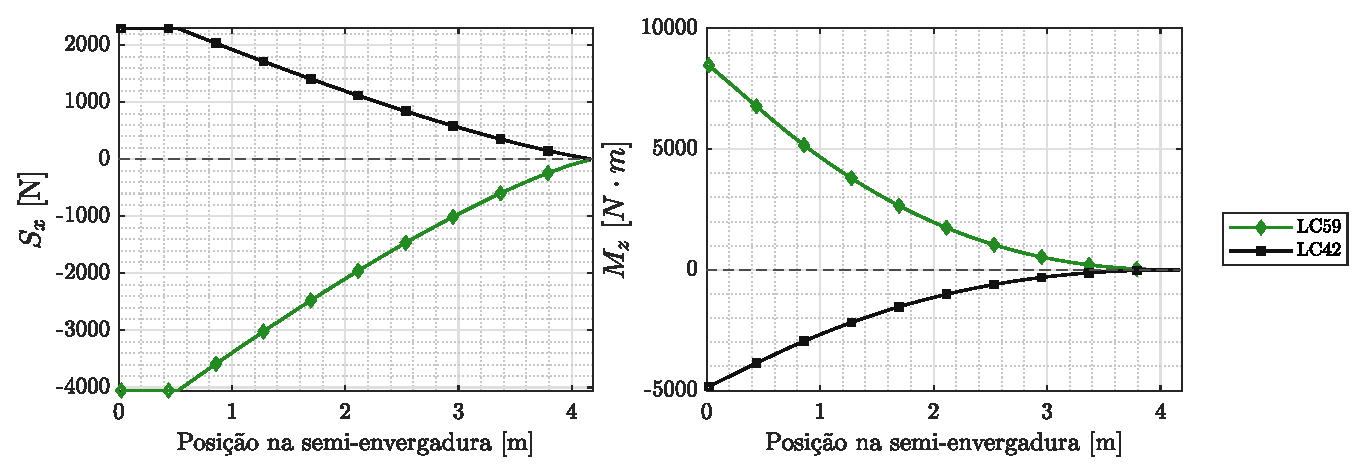
\includegraphics[width=0.91\linewidth]{images/cargas/esforcos_Fx_eh.eps}
    \caption{Esforços críticos associados a $F_x$ na EH.}
    \label{fig:cargas_eh_crit_fx}
\end{figure}

\begin{figure}[H]
    \centering
    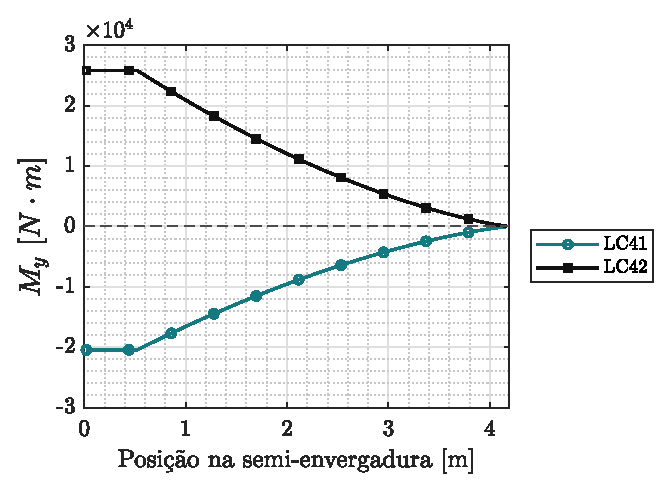
\includegraphics[width=0.55\linewidth]{images/cargas/esforco_MA_eh.eps}
    \caption{Momento torsor crítico $M_y$ na EH.}
    \label{fig:cargas_eh_crit_my}
\end{figure}

\section{Cargas na EV}
\label{sec:cargas_ev}

As cargas da EV foram determinadas para condições de manobra de guinada e rajada lateral. Os carregamentos resultantes foram distribuídos ao longo da altura da EV pelo método de Stender, permitindo a determinação dos esforços internos.

\subsection*{Manobras}

As cargas de manobra foram estimadas com referência ao \S~25.351 do 14 CFR Part 25, considerando a deflexão máxima do leme sem derrapagem e as condições de derrapagem, incluindo o leme neutro. A força lateral foi calculada pela contribuição do ângulo de derrapagem $\beta$ e da deflexão do leme $\zeta$:
\begin{equation}
    C_{L,vt}=a_{vt}\beta+C_{L,vt,\zeta}\zeta,
    \qquad
    L_{vt}=\frac{1}{2}\rho_0V_{\mathrm{EAS}}^2S_{vt}C_{L,vt}.
    \label{eq:cargas_ev_man}
\end{equation}

\subsection*{Rajada}

As cargas de rajada lateral foram estimadas com referência ao \S~25.341 do 14 CFR Part 25, considerando os dois sentidos de incidência da rajada e o fator de alívio adotado no cálculo. O incremento de força lateral foi determinado por
\begin{equation}
    \Delta L_{vt,g}=\frac{1}{2}\rho_0V_{\mathrm{EAS}}S_{vt}
    \left|a_{vt}\right|U_gK_{g,vt}.
    \label{eq:cargas_ev_raj}
\end{equation}

\subsection*{Arrasto, Momento Aerodinâmico e Distribuição}

O arrasto da EV foi estimado a partir da sustentação local e da polar bidimensional do perfil adotado. Para o momento aerodinâmico, utilizou-se a mesma aproximação empregada na EH, com as distribuições das Figuras B6, B7 e B8 do Apêndice B da CS-VLA, referidas a $25\%$ da corda local. Essas distribuições foram adotadas como estimativa preliminar, sem alterar a base normativa de categoria Transporte da aeronave.

As parcelas de força lateral, arrasto e momento aerodinâmico da região não exposta junto à fuselagem foram redistribuídas sobre os trechos externos da EV. As componentes nos eixos da aeronave foram obtidas por
\begin{align}
    F_y &= L_{vt}\cos\beta-D_{vt}\sin\beta, \\
    F_x &= L_{vt}\sin\beta+D_{vt}\cos\beta.
    \label{eq:cargas_transform_ev}
\end{align}

\subsection*{Resultados}

Os carregamentos distribuídos obtidos pelo método de Stender são apresentados na \autoref{fig:cargas_ev_fy}, na \autoref{fig:cargas_ev_fx} e na \autoref{fig:cargas_ev_ma}.

\begin{figure}[H]
    \centering
    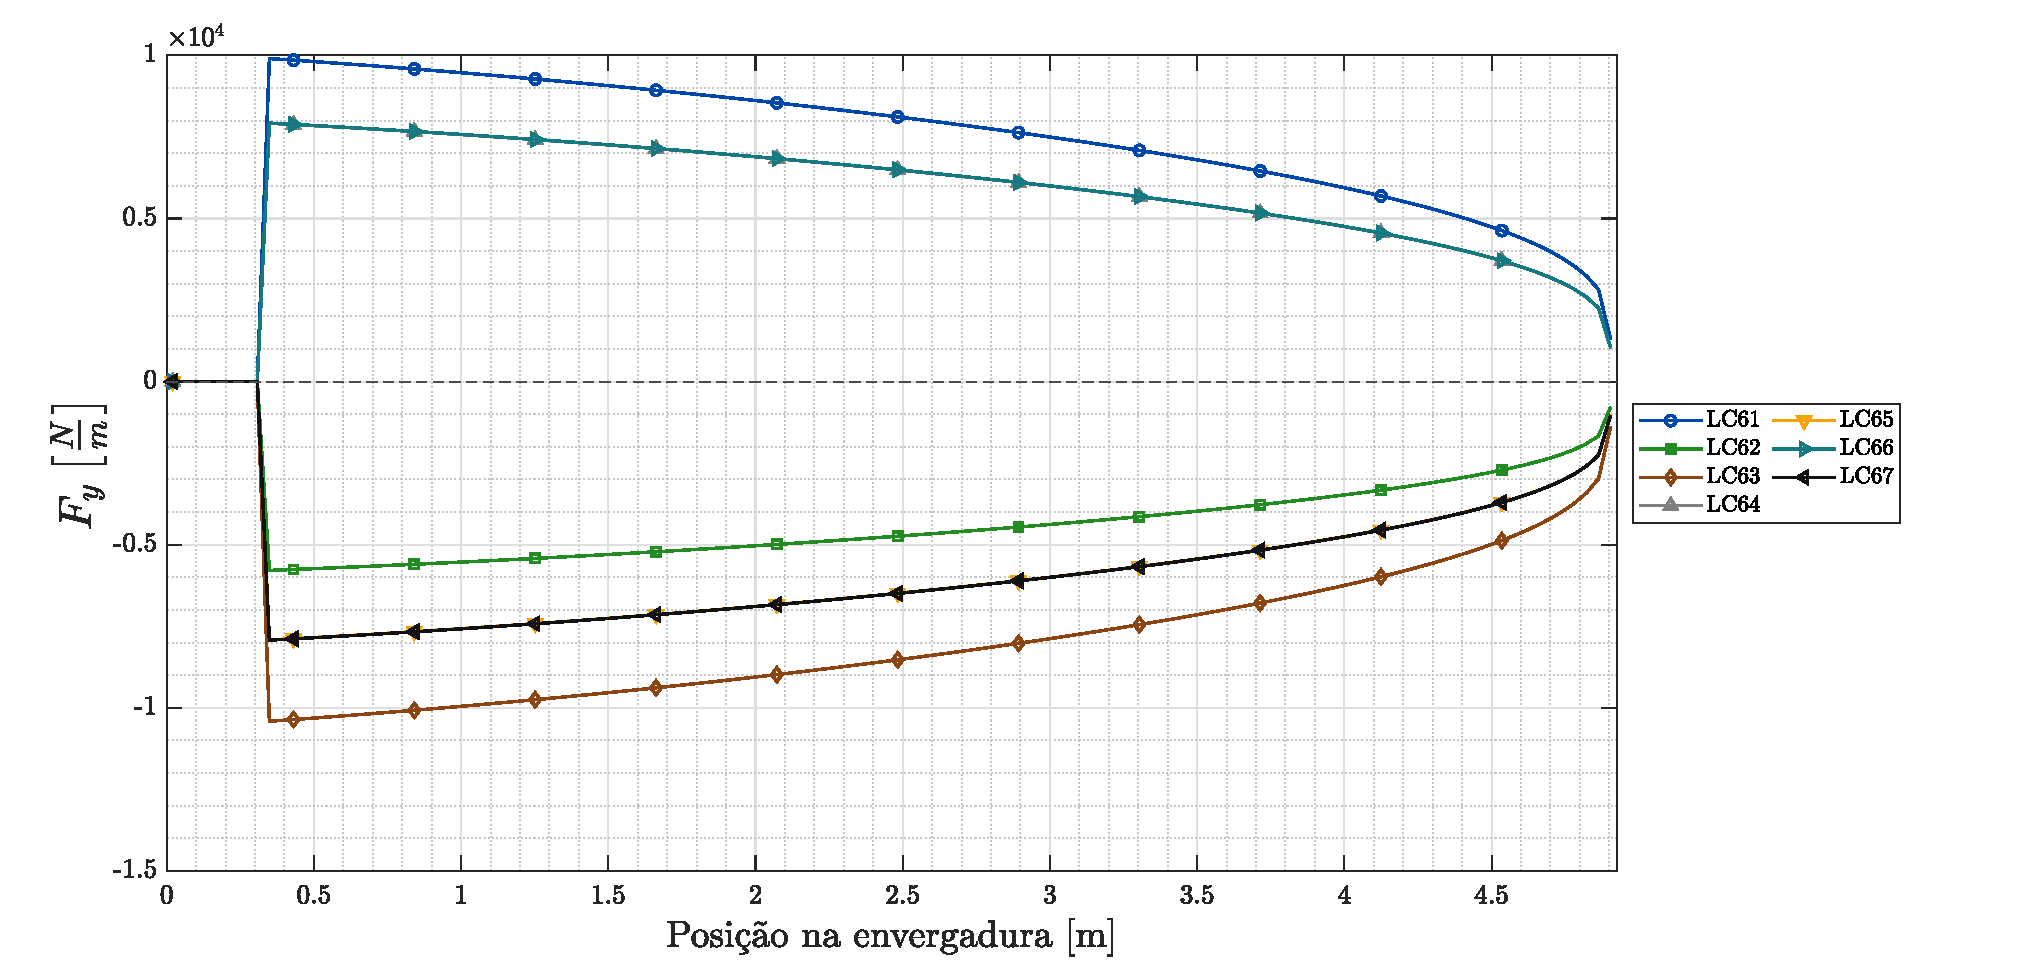
\includegraphics[width=1\linewidth]{images/cargas/vtail_Fy.eps}
    \caption{$F_y$ distribuído na EV.}
    \label{fig:cargas_ev_fy}
\end{figure}

\begin{figure}[H]
    \centering
    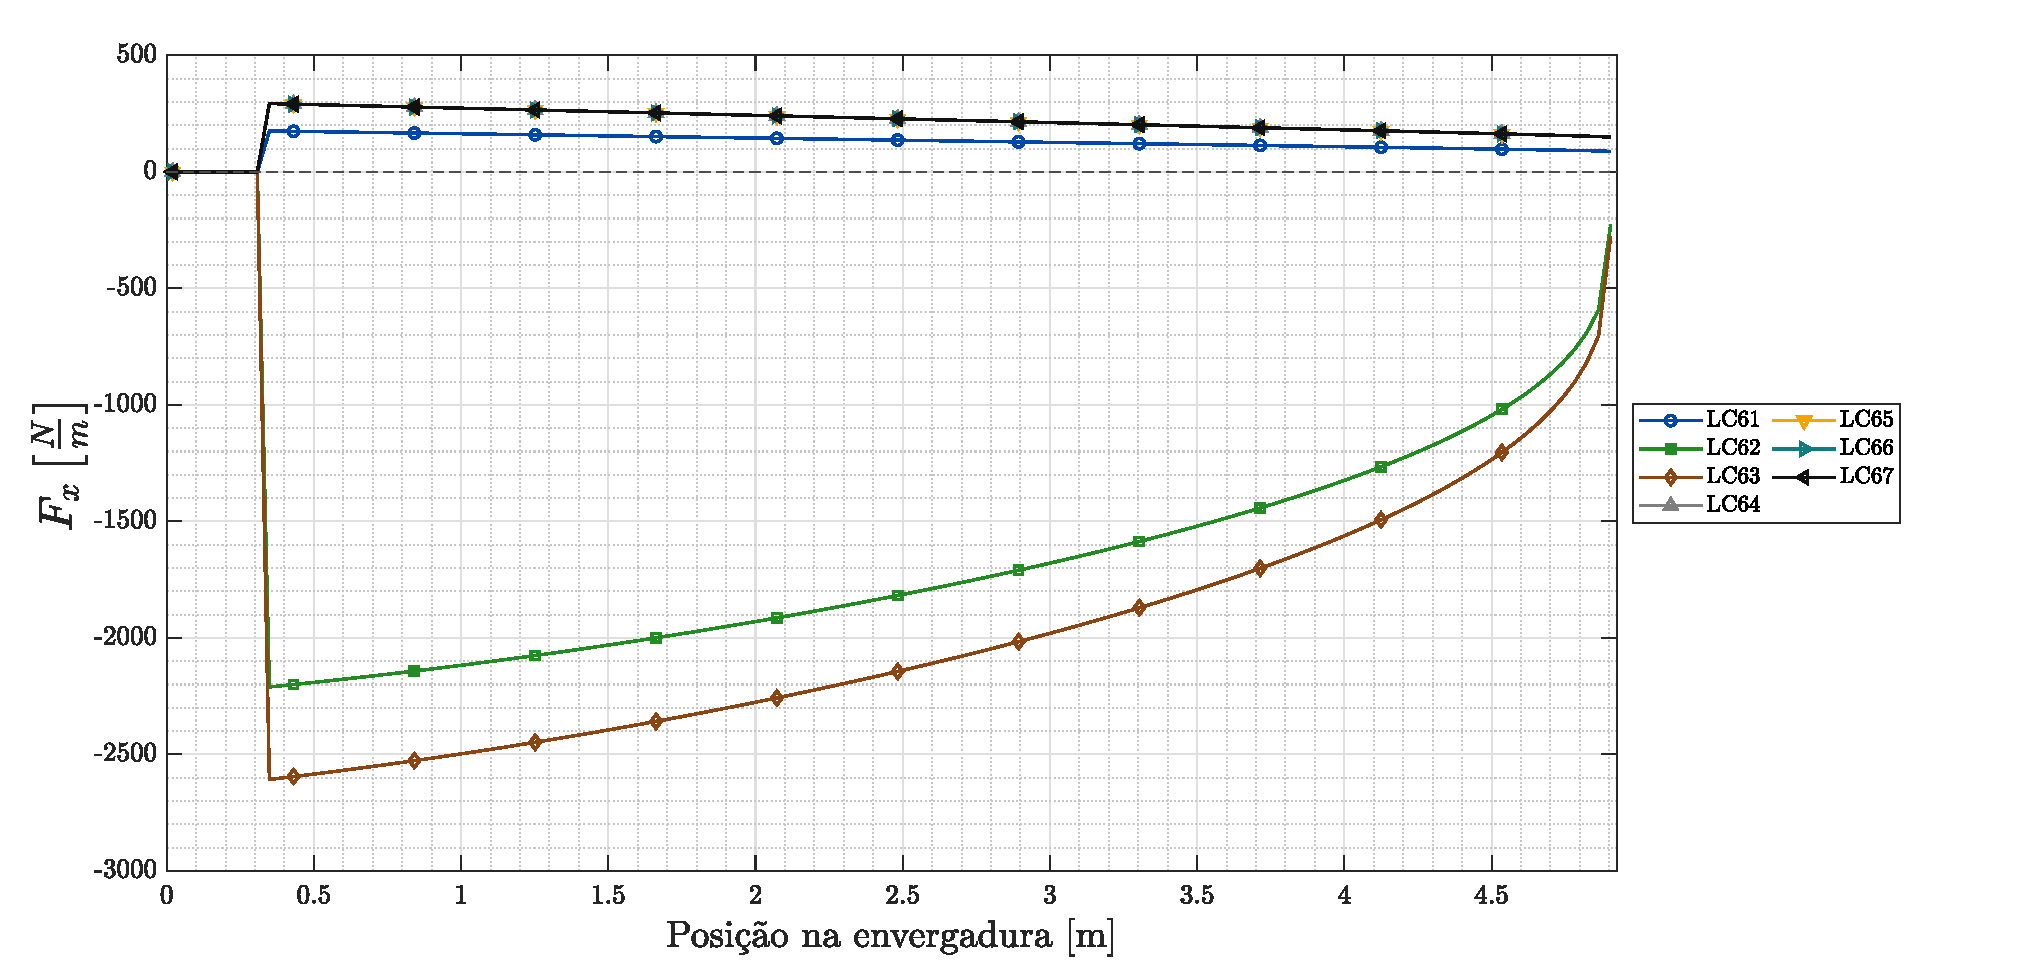
\includegraphics[width=1\linewidth]{images/cargas/vtail_Fx.eps}
    \caption{$F_x$ distribuído na EV.}
    \label{fig:cargas_ev_fx}
\end{figure}

\begin{figure}[H]
    \centering
    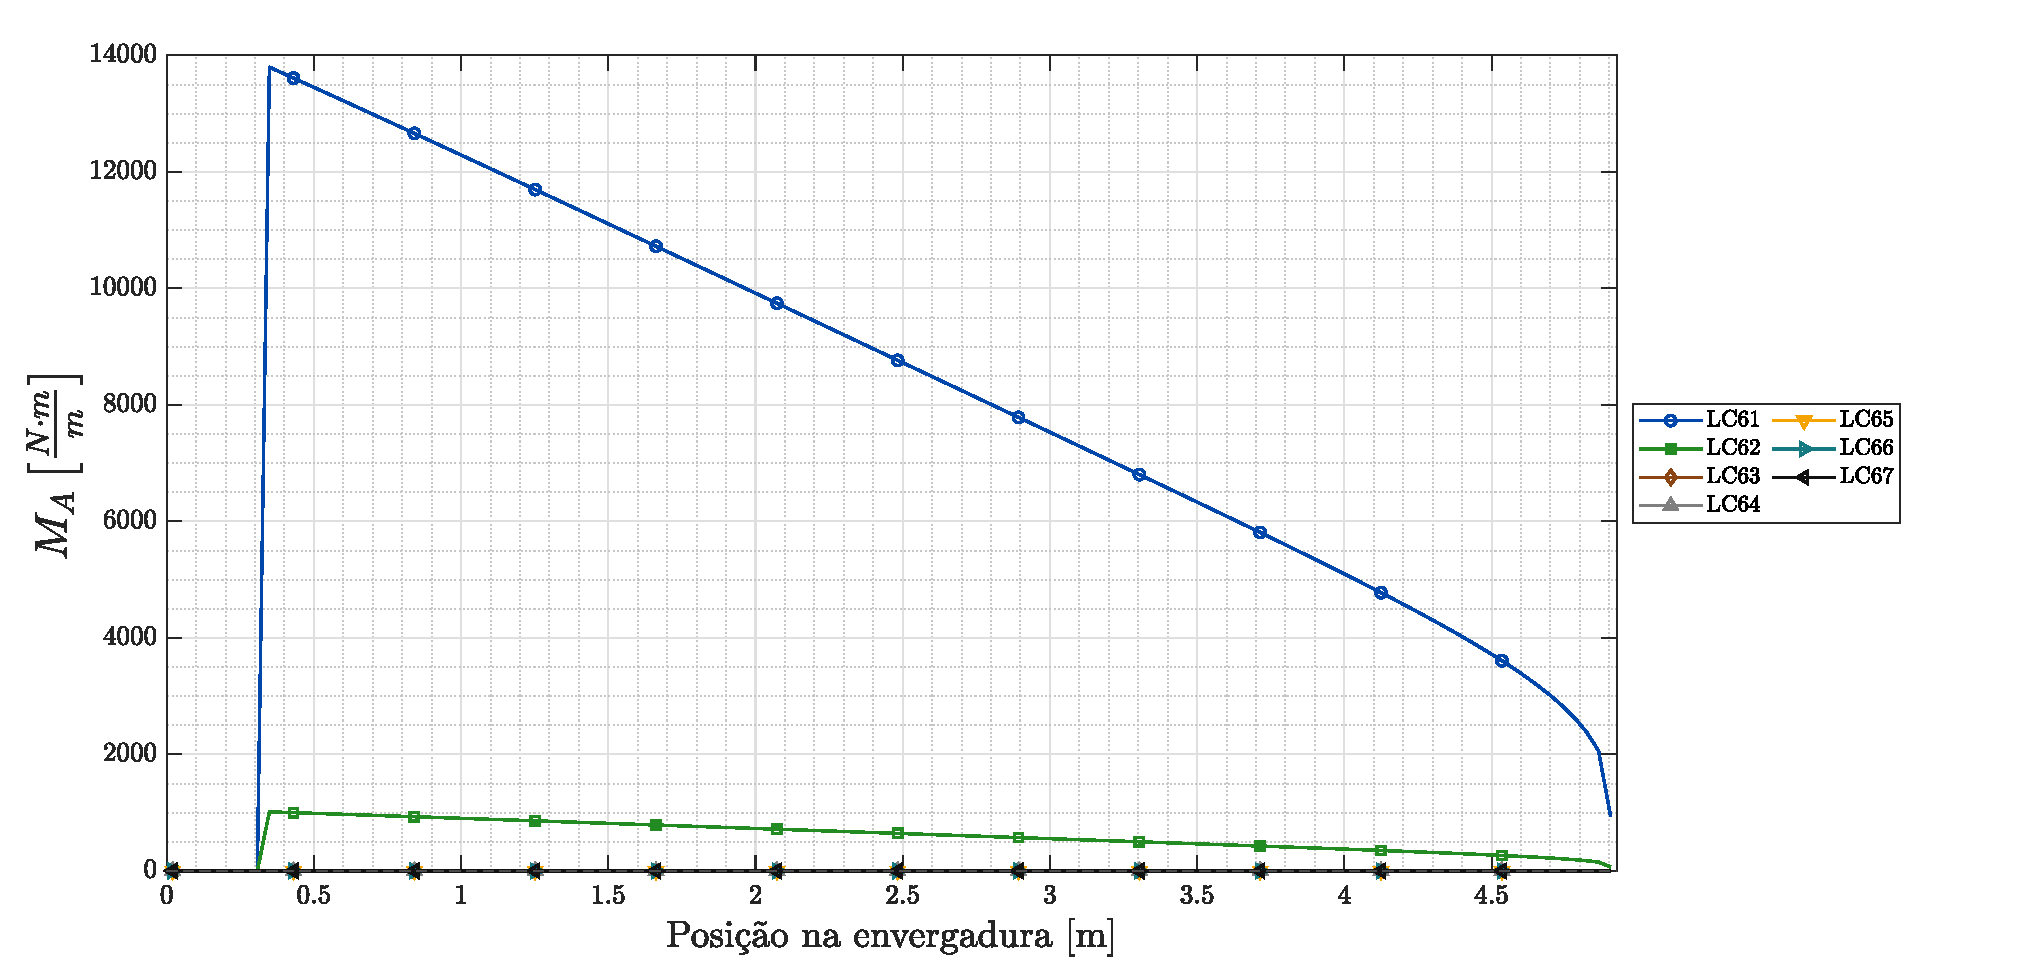
\includegraphics[width=1\linewidth]{images/cargas/vtail_MA.eps}
    \caption{$MA$ distribuído na EV.}
    \label{fig:cargas_ev_ma}
\end{figure}

As condições de voo correspondentes aos casos críticos identificados para a EV são resumidas na Tabela~\ref{tab:cargas_criticas_ev}.

\begin{table}[H]
    \centering
    \caption{Condições críticas da EV.}
    \label{tab:cargas_criticas_ev}
    \vspace{1mm}
    \begingroup
    \footnotesize
    \setlength{\tabcolsep}{5pt}
    \renewcommand{\arraystretch}{1.35}
    \begin{tabular}{@{}lccccccc@{}}
        \noalign{\hrule height 0.8pt}
        \textbf{N\textsuperscript{o}} & \textbf{Tipo} & \textbf{14 CFR Part 25} & \textbf{TOW} & \textbf{CG} & \textbf{Flap} & \textbf{Velocidade} & \textbf{Condição}\\
        \hline
        LC61 & Manobra & \S~25.351 & MTOW & --- & Recolhido & $V_A$ & $\zeta=+30^\circ$\\
        LC63 & Manobra & \S~25.351 & MTOW & --- & Recolhido & $V_A$ & $\beta=15^\circ$\\
        LC66 & Rajada & \S~25.341 & MTOW & Traseiro & Recolhido & $V_C$ & Rajada (+)\\
        \noalign{\hrule height 0.8pt}
    \end{tabular}
    \endgroup
\end{table}

Os esforços internos correspondentes às condições críticas são apresentados na \autoref{fig:cargas_ev_crit_fy}, na \autoref{fig:cargas_ev_crit_fx} e na \autoref{fig:cargas_ev_crit_mz}.

%% Os gráficos de esforços abaixo incluem SOMENTE as condições críticas.
\begin{figure}[H]
    \centering
    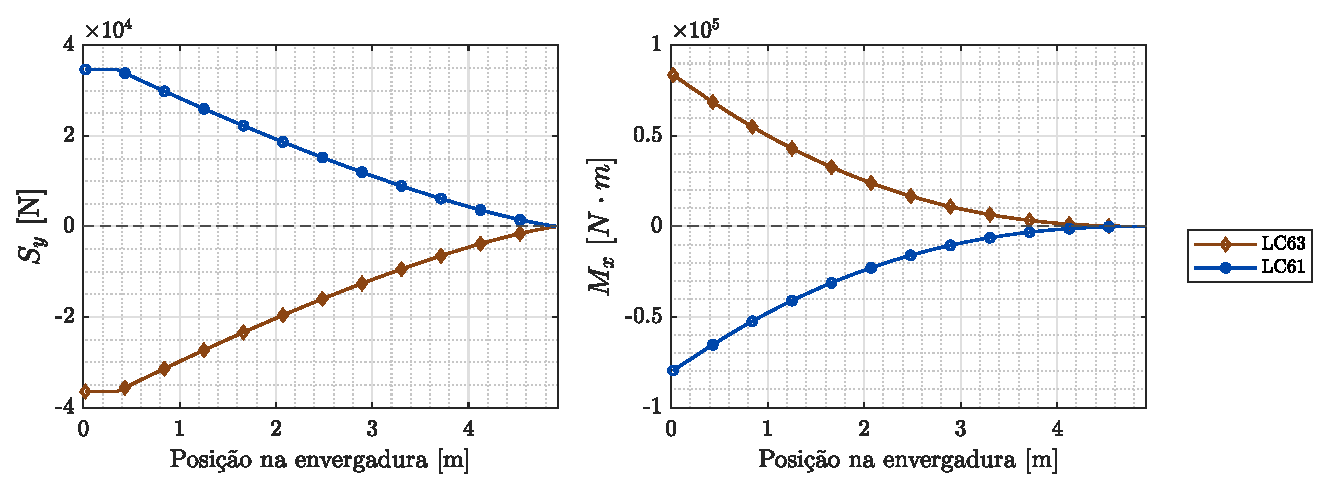
\includegraphics[width=0.91\linewidth]{images/cargas/esforcos_Fy_ev.eps}
    \caption{Esforços críticos associados a $F_y$ na EV.}
    \label{fig:cargas_ev_crit_fy}
\end{figure}

\begin{figure}[H]
    \centering
    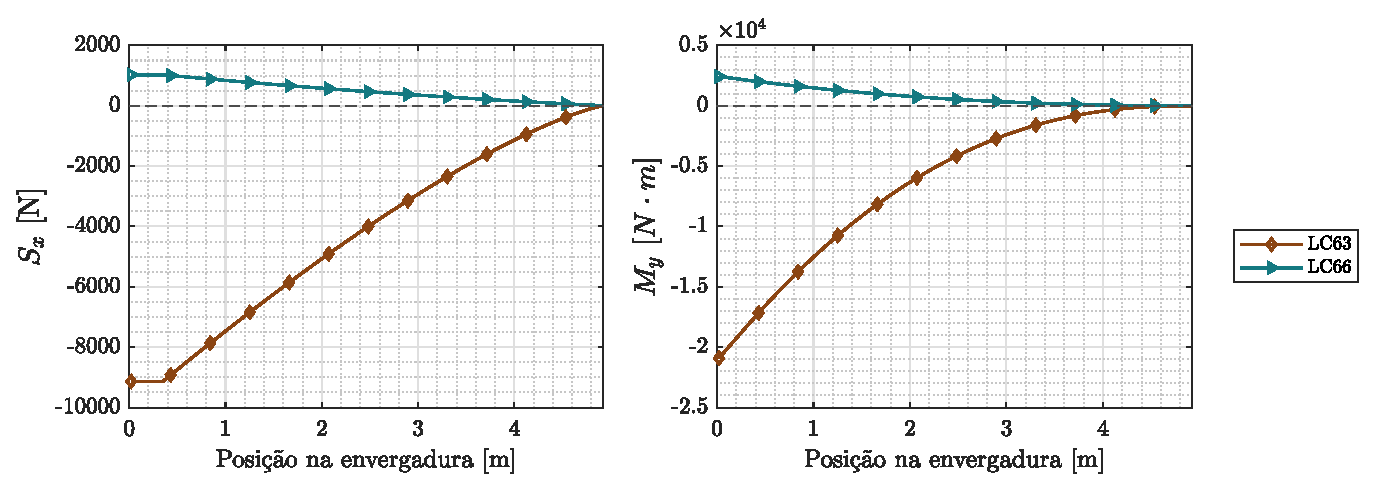
\includegraphics[width=0.91\linewidth]{images/cargas/esforcos_Fx_ev.eps}
    \caption{Esforços críticos associados a $F_x$ na EV.}
    \label{fig:cargas_ev_crit_fx}
\end{figure}

\begin{figure}[H]
    \centering
    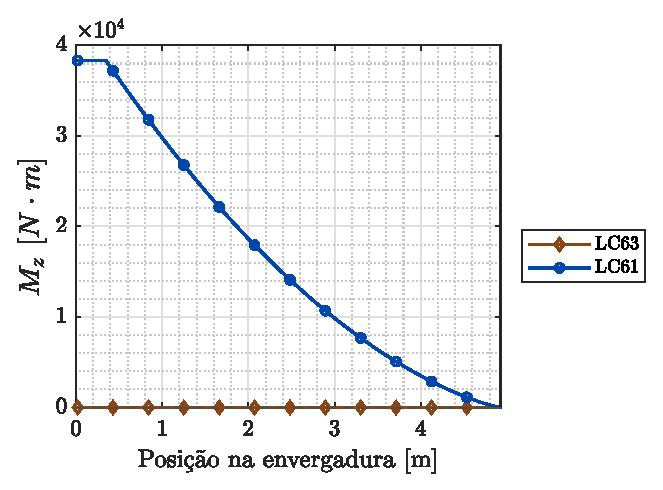
\includegraphics[width=0.55\linewidth]{images/cargas/esforco_MA_ev.eps}
    \caption{Momento torsor crítico $M_z$ na EV.}
    \label{fig:cargas_ev_crit_mz}
\end{figure}

Vale ressaltar que as manobras da empenagem vertical são simétricas em relação ao plano longitudinal da aeronave. Dessa forma, os casos foram avaliados em apenas um sentido, sendo o envelope de cargas considerado equivalente para o sentido oposto.

\section{Cargas no Trem de Pouso}
\label{sec:cargas_solo}


A determinação das cargas atuantes no trem de pouso durante as operações de toque e rolagem foi realizada considerando cinco condições críticas de pouso. De modo análogo às simplificações preliminares adotadas nas seções anteriores para as empenagens, recorreu-se à metodologia analítica simplificada prescrita nas seções \S 23.479 a \S 23.485 e no Apêndice C do 14 CFR Part 23 (correspondentes às condições equivalentes das seções \S 25.479 a \S 25.485 do 14 CFR Part 25 e RBAC 25). Essa abordagem permite estimar as reações estáticas equivalentes nas pernas do trem de pouso principal (TDPP) e do trem de pouso auxiliar de nariz (TDPA) sem exigir, nesta fase do projeto preliminar, a modelagem dinâmica não-linear dos amortecedores óleo-pneumáticos, mantendo-se inalterada a base certificadora da aeronave na Categoria Transporte.

\subsubsection*{Sistema de Coordenadas e Parâmetros de Entrada}

% A geometria das pernas do trem de pouso é referenciada ao Centro de Gravidade (CG) da aeronave no sistema de eixos de corpo, no qual o eixo $+x_b$ aponta para a frente, $+y_b$ para a semiasa direita e $+z_b$ verticalmente para baixo. As coordenadas do ponto de contato de cada conjunto com o solo em relação ao CG são definidas pelos vetores posição $\vec{r}_{\text{TDPP}} = [x_m, \, y_m, \, z_m]$ e $\vec{r}_{\text{TDPA}} = [x_n, \, 0, \, z_n]$.

% Por sua vez, as reações de contato provenientes do solo sobre os pneus são expressas no referencial de cargas de saída, adotando-se o eixo $+X$ orientado longitudinalmente para trás (sentido da força de arrasto de \textit{spin-up} das rodas), $+Y$ lateralmente para a direita e $+Z$ verticalmente para cima (reação normal à pista).

% Os cálculos foram conduzidos para a condição crítica de Peso Máximo de Decolagem ($\text{MTOW} = 22\,680\text{ kg}$, correspondente a $W = \text{MTOW} \cdot g$).
Adotou-se um fator de carga inercial limite vertical no CG igual a $n_{\text{inertia}} = 2,67$ e uma fração máxima de sustentação aerodinâmica remanescente no instante do toque de $k_L = L/W = 2/3$. Dessa forma, o fator de carga vertical líquido transmitido ao solo ($n_{\text{ground}}$) nas condições simétricas de impacto é dado por:
\begin{equation}
    n_{\text{ground}} = n_{\text{inertia}} - k_L = 2,00.
    \label{eq:n_ground}
\end{equation}

Adicionalmente, a razão entre a componente longitudinal de arrasto e a reação vertical ($D/V$) decorrente da aceleração rotacional das rodas no toque é $K = 0,33$ do Apêndice C da norma, resultando em:
\begin{equation}
    r_{DV} = \frac{K \, n_{\text{inertia}}}{n_{\text{ground}}}.
    \label{eq:r_dv}
\end{equation}

\subsubsection*{Condições de Carregamento Avaliadas}

A seguir, detalham-se as hipóteses físicas e as equações de equilíbrio estático aplicadas a cada um dos cinco casos de carga (\textit{Load Cases}) implementados computacionalmente:

\begin{itemize}
    \item \textbf{Condição C1 -- Pouso em três rodas:} Considera a aeronave em atitude nivelada com toque simultâneo dos trens principal e de nariz.
    \begin{equation}
        F_{z,\text{TDPA}} = W \, n_{\text{ground}} \, \frac{-x_m + r_{DV} \, z_n}{x_n - x_m},
        \label{eq:c1_nose_z}
    \end{equation}
    \begin{equation}
        F_{z,\text{TDPP1}} = F_{z,\text{TDPP2}} = \frac{1}{2} \, W \, n_{\text{ground}} \, \frac{x_n - r_{DV} \, z_m}{x_n - x_m}.
        \label{eq:c1_main_z}
    \end{equation}
    As componentes longitudinais atuantes em cada perna são proporcionais às respectivas cargas normais ($F_x = r_{DV} \, F_z$), totalizando uma força longitudinal de arrasto $D_{\text{tot}} = K \, n_{\text{inertia}} \, W$, enquanto as componentes laterais são nulas ($F_y = 0$).

    \item \textbf{Condição C2 -- Pouso em duas rodas nivelado :} A aeronave encontra-se em atitude longitudinal nivelada, porém o contato ocorre exclusivamente pelas duas pernas do trem de pouso principal ($\vec{F}_{\text{TDPA}} = \vec{0}$).
    \begin{equation}
        F_{z,\text{TDPP1}} = F_{z,\text{TDPP2}} = \frac{1}{2} \, n_{\text{ground}} \, W, \qquad F_{x,\text{TDPP1}} = F_{x,\text{TDPP2}} = r_{DV} \, F_{z,\text{TDPP1}}.
        \label{eq:c2_loads}
    \end{equation}

    \item \textbf{Condição C3 -- Pouso em duas rodas com cauda abaixada :} Representa o toque na atitude de máximo ângulo de ataque (estol ou próximo ao estol), com contato restrito às rodas principais ($\vec{F}_{\text{TDPA}} = \vec{0}$). Nessa configuração geométrica, a resultante de impacto atua na direção vertical pura, de modo que as componentes longitudinais e laterais são nulas:
    \begin{equation}
        F_{z,\text{TDPP1}} = F_{z,\text{TDPP2}} = \frac{1}{2} \, n_{\text{ground}} \, W, \qquad F_{x} = F_{y} = 0.
        \label{eq:c3_loads}
    \end{equation}

    \item \textbf{Condição C4 -- Pouso em uma roda :} Simula uma aterrissagem assimétrica com inclinação lateral, na qual apenas uma das pernas do trem principal (adotada como TDPP1, lado direito) toca a pista, enquanto a perna oposta e o trem de nariz permanecem livres ($\vec{F}_{\text{TDPP2}} = \vec{F}_{\text{TDPA}} = \vec{0}$).
    \begin{equation}
        F_{z,\text{TDPP1}} = \frac{1}{2} \, n_{\text{ground}} \, W, \qquad F_{x,\text{TDPP1}} = r_{DV} \, F_{z,\text{TDPP1}}, \qquad F_{y,\text{TDPP1}} = 0.
        \label{eq:c4_loads}
    \end{equation}

    \item \textbf{Condição C5 -- Pouso em duas rodas com carga lateral:} Avalia o toque em atitude nivelada sob efeito de derrapagem.
    \begin{equation}
        F_{z,\text{TDPP1}} = F_{z,\text{TDPP2}} = \frac{1}{2} \, n_{g,\text{side}} \, W,
        \label{eq:c5_z}
    \end{equation}
    \begin{equation}
        F_{y,\text{TDPP1}} = -0,50 \, W, \qquad F_{y,\text{TDPP2}} = -0,33 \, W.
        \label{eq:c5_y}
    \end{equation}
\end{itemize}

\subsubsection*{Resultados}

As componentes de força nos eixos $X$, $Y$ e $Z$ obtidas para o Trem de Pouso Principal direito (TDPP1), Trem de Pouso Principal esquerdo (TDPP2) e Trem de Pouso Auxiliar de nariz (TDPA) em cada uma das cinco condições analisadas encontram-se consolidadas na Tabela~\ref{tab:cargas_pouso}.

\begin{table}[H]
\centering
\caption{Cargas limite atuantes no trem de pouso por condição de operação.}
\label{tab:cargas_pouso}
\setlength{\tabcolsep}{4.5pt}
\renewcommand{\arraystretch}{1.2}
\resizebox{\textwidth}{!}{%
\begin{tabular}{c l r r r r r r r r r}
\hline
\textbf{Cond.} & \textbf{Descrição} & \multicolumn{3}{c}{\textbf{TDPP 1 (Dir.) [kN]}} & \multicolumn{3}{c}{\textbf{TDPP 2 (Esq.) [kN]}} & \multicolumn{3}{c}{\textbf{TDPA (Nariz) [kN]}} \\
 & & \multicolumn{1}{c}{$F_x$} & \multicolumn{1}{c}{$F_y$} & \multicolumn{1}{c}{$F_z$} & \multicolumn{1}{c}{$F_x$} & \multicolumn{1}{c}{$F_y$} & \multicolumn{1}{c}{$F_z$} & \multicolumn{1}{c}{$F_x$} & \multicolumn{1}{c}{$F_y$} & \multicolumn{1}{c}{$F_z$} \\
\hline
\textbf{C1} & Pouso em três rodas & 91,53 & 0,00 & 207,90 & 91,53 & 0,00 & 207,90 & 13,01 & 0,00 & 29,54 \\
\textbf{C2} & Pouso em duas rodas nivelado & 97,80 & 0,00 & 222,14 & 97,80 & 0,00 & 222,14 & 0,00 & 0,00 & 0,00 \\
\textbf{C3} & Pouso em duas rodas cauda abaixada & 0,00 & 0,00 & 222,14 & 0,00 & 0,00 & 222,14 & 0,00 & 0,00 & 0,00 \\
\textbf{C4} & Pouso em uma roda & 97,80 & 0,00 & 222,14 & 0,00 & 0,00 & 0,00 & 0,00 & 0,00 & 0,00 \\
\textbf{C5} & Pouso em duas rodas com carga lateral & 0,00 & -111,21 & 147,91 & 0,00 & -73,40 & 147,91 & 0,00 & 0,00 & 0,00 \\
\hline
\end{tabular}%
}
\end{table}

A análise da Tabela~\ref{tab:cargas_pouso} evidencia que a solicitação vertical máxima no trem de pouso principal ocorre nas condições C2, C3 e C4, atingindo uma reação normal de $222\,136,52\text{ N}$ por perna, acompanhada de uma força longitudinal máxima de arrasto (\textit{spin-up}) de $97\,798,37\text{ N}$ nas condições C2 e C4. No que tange aos esforços laterais, a Condição C5 impõe o carregamento crítico de derrapagem, resultando em forças de $-111\,207,41\text{ N}$ na perna direita (TDPP1) e $-73\,396,89\text{ N}$ na perna esquerda (TDPP2). Por sua vez, o trem de pouso auxiliar de nariz (TDPA) atinge seu carregamento dimensionante na Condição C1 (pouso nivelado em três rodas), suportando uma carga limite vertical de $29\,541,51\text{ N}$ e longitudinal de $13\,006,07\text{ N}$.
\chapter{Dimensionamento Estrutural}
\label{dimensionamento_estrutural}

\section{Materiais de Construção}

\begin{figure}[H]
    \centering
    \begin{minipage}{1\textwidth} % Ajuste o 0.8 para aumentar ou diminuir o tamanho
        \centering
        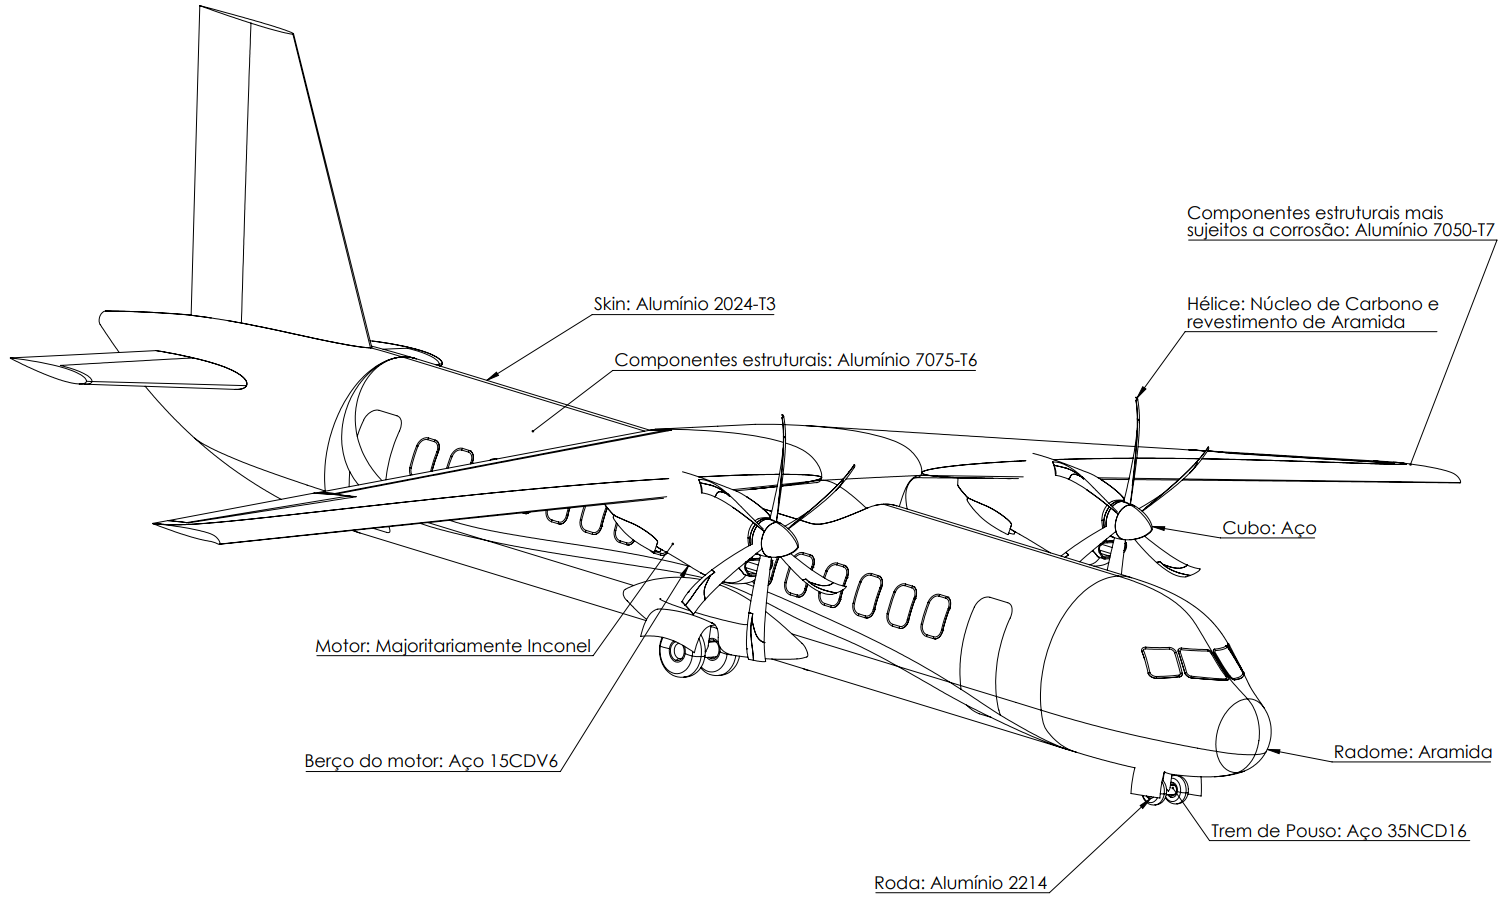
\includegraphics[width=\linewidth]{images/Materiais da aeronave.png}
        \caption{Materiais constituintes da aeronave.}
        \label{fig:Materiais da aeronave}
    \end{minipage}
\end{figure}

%Os materiais que constituem a aeronave foram escolhidos principalmente em relação às suas características serem compatíveis ao seu respectivo uso, mas houve grande inspiração nas aeronaves descritas na análise comparativa.

O radome da aeronave é fabricado em material compósito por aramida em estrutura sanduíche. Apesar de ter grande propensão ao acúmulo de água, é excelente em suportar colisões. Ademais, não interfere nas medições do radar meteorológico, posicionado logo abaixo.

Já no trem de pouso, as rodas são constituídas de uma liga de alumínio forjado 2214, com alto teor de cobre, além de ser leve, é dúctil a fim de suportar os impactos do pouso. A estrutura do trem de pouso em si é de aço 35NCD16, que tem níquel, cromo e molibdênio em sua composição, sendo altamente resistente à corrosão, já que está mais exposta, apesar do banho de proteção normalmente de cádmio; e à fadiga decorrente dos impactos durante o pouso.

No GMP, o motor PW127 é composto majoritariamente de ligas Inconel da classe 600 e 800, que são superligas de níquel. Já a hélice Hamilton Standard 568F tem pás com núcleo de carbono e revestimento de aramida, para maior resistência a danos por impacto. O cubo da hélice é de aço devido aos altos torques. Entretanto, a Hamilton não disponibiliza a liga. Por último, o berço do motor é composto por uma estrutura tubular em aço 15CDV6, pela capacidade construtiva, uma vez que apresenta excelente soldabilidade.

A célula e as superfícies sustentadoras são fabricadas em alumínio. As longarinas, nervuras, cavernas, reforçadores e longerons são de alumínio 7075-T6, que apresenta a maior resistência específica. Já em partes mais expostas, como em trilhos de fixação, será utilizada a liga 7050-T7, que apresenta melhor resistência à corrosão. O revestimento (\textit{skin}) da aeronave é composta por 2024-T3 ALCLAD, por ser mais trabalhável, podendo alcançar baixas espessuras mantendo a resistência.

A Tabela \ref{tab:propriedades_aluminio_si} sintetiza as propriedades das ligas utilizadas no dimensionamento estrutural.

\begin{table}[H]
\centering
\caption{Propriedades mecânicas das ligas de alumínio em unidades básicas do SI.}
\label{tab:propriedades_aluminio_si}
\begin{tabular}{|l|c|c|c|c|c|}
\hline
\textbf{Material} & \textbf{$E$ [GPa]} & \textbf{$\rho$ [kg/m$^3$]} & \textbf{$\nu$} & \textbf{$F_{ty}$ [MPa]} & \textbf{$F_{tu}$ [MPa]} \\ \hline
2024-T3 & $72,394$ & 2780 & 0,33 & $324,054$ & $441,264$ \\ \hline
7075-T6 & $71,016$ & 2810 & 0,33 & $503,317$ & $572,265$ \\ \hline
\end{tabular}
\end{table}

% A estrutura preliminar na fuselagem está ilustrada na imagem abaixo.

% \begin{figure}[H]
%     \centering
%     \begin{minipage}{1\textwidth} % Ajuste o 0.8 para aumentar ou diminuir o tamanho
%         \centering
%         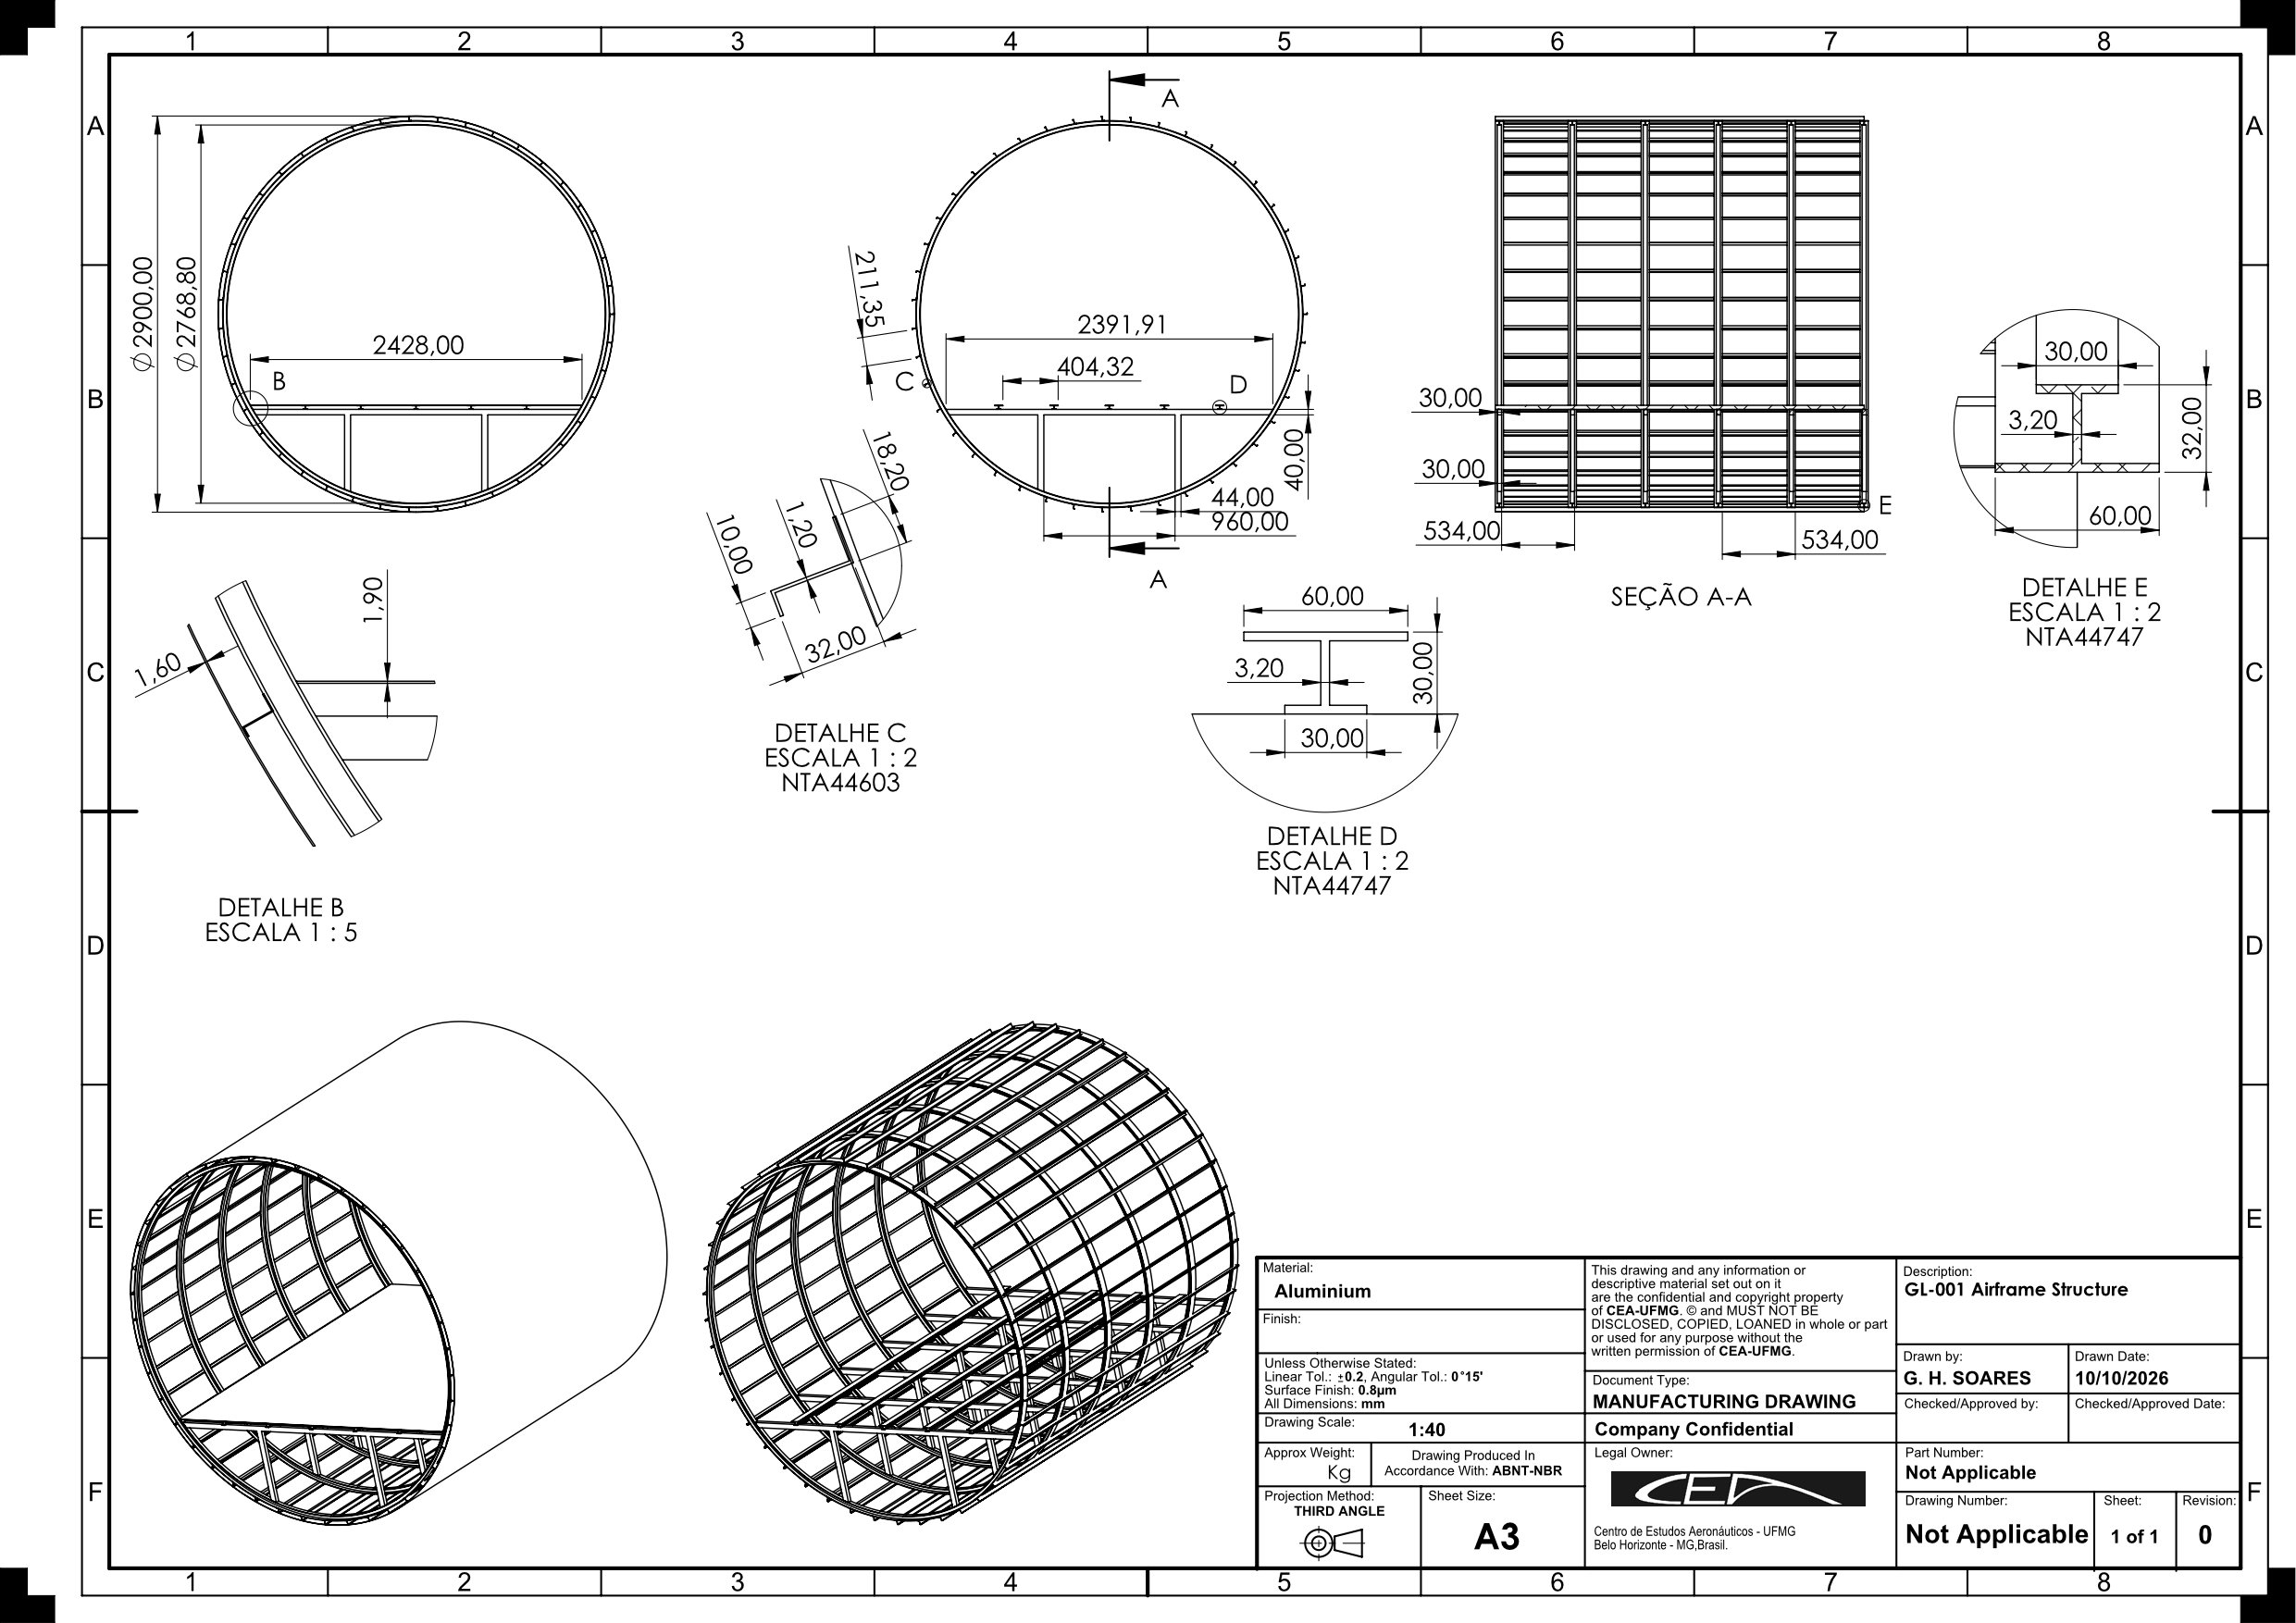
\includegraphics[width=\linewidth]{images/Estrutura interna da fuselagem2.jpg}
%         \caption{Estrutura interna da fuselagem.}
%         \label{fig:Estrutura interna da fuselagem}
%     \end{minipage}
% \end{figure}

\section{Asa}
\subsection{Longarina}
\label{sec:secao_longarina_asa}

O dimensionamento da longarina principal da asa utiliza uma seção transversal em formato I. Essa geometria apresenta eficiência estrutural para resistir aos esforços de flexão verticais, pois afasta o material da linha neutra, aumentando o momento de inércia da área. Essa distribuição de material permite a obtenção de uma estrutura com massa reduzida em comparação com seções retangulares maciças, por exemplo. 

A adoção dessa geometria estrutural mantém a consistência com as etapas prévias do projeto. Em capítulos anteriores, a seção em I já havia sido estipulada durante os cálculos preliminares associados à geometria do perfil aerodinâmico (seção 7.1.3) e à determinação da altura disponível no interior da asa. Dessa forma, o detalhamento estrutural atual parte das premissas e dos parâmetros dimensionais que foram estabelecidos ao longo do desenvolvimento aerodinâmico da aeronave.

A longarina é posicionada na coordenada de máxima espessura dos perfis aerodinâmicos ao longo de toda a envergadura. Essa localização maximiza a altura da seção transversal, resultando em um maior momento de inércia e no aumento da resistência aos esforços de flexão. Para a determinação da altura efetiva disponível para a estrutura, a espessura do revestimento externo é descontada das ordenadas do perfil aerodinâmico, permitindo a acomodação dimensional do conjunto.

O material selecionado para a longarina é a liga de alumínio 7075-T6, cujas propriedades mecânicas são compatíveis com os requisitos de projeto de elementos estruturais primários. Os parâmetros empregados no dimensionamento estão sumarizados na Tabela \ref{tab:rev_materiais}.

O dimensionamento estrutural avalia os esforços de momento fletor e de esforço cortante ao longo da envergadura. Para a asa, a análise abrange três casos de carga críticos: o caso LC4, o caso LC5 e o caso LC11.

A seção transversal em I é analisada em três pontos de interesse para a determinação do estado de tensões: a borda da mesa, a junção entre a mesa e a alma, e a linha neutra. A tensão equivalente em cada um desses pontos é avaliada com base no critério de falha de von Mises, calculado por meio da seguinte equação:

$$\sigma_{VM} = \sqrt{\sigma^2 + 3\tau^2}$$

em que $\sigma$ representa a tensão normal e $\tau$ a tensão de cisalhamento.

Os critérios de resistência adotados fundamentam-se nos requisitos do regulamento FAR/CS 25, em particular nas seções 25.303 e 25.305. A norma exige que a estrutura não apresente deformação permanente sob a aplicação das cargas limites. Desse modo, para o carregamento limite, impõe-se que a tensão equivalente não ultrapasse o limite de escoamento do material ($\sigma_{VM} \le F_{ty}$). O regulamento também estabelece que a estrutura deve ser capaz de suportar as cargas últimas sem sofrer ruptura. As cargas últimas são obtidas pela multiplicação das cargas limites por um \textbf{fator de segurança de 1,5}. Para esta condição, a tensão equivalente deve ser inferior ao limite de ruptura do material ($\sigma_{VM} \le F_{tu}$).

O parâmetro utilizado para quantificar o atendimento a esses critérios estruturais é a Margem de Segurança (MS), definida como:

$$MS = \frac{\text{tensão admissível}}{\sigma_{VM}} - 1$$

Para que o dimensionamento seja aprovado nos critérios de escoamento e de ruptura, exige-se que $MS \ge 0$.

No trecho da longarina compreendido entre a nacele e a ponta da asa, as dimensões da seção transversal são reduzidas de forma gradativa. A largura das mesas e as espessuras da alma e das mesas variam linearmente ao longo da envergadura, enquanto a altura da seção acompanha a geometria do perfil aerodinâmico local. O processo de dimensionamento avalia as margens de segurança de maneira iterativa ao longo desse segmento. Caso alguma estação apresente uma margem de segurança negativa, as espessuras estipuladas para a ponta da asa são incrementadas computacionalmente até que os requisitos de resistência sejam atendidos nas estações avaliadas.

O dimensionamento do trecho de seção constante, compreendido entre a raiz e a nacele, adotou uma largura de mesa ($b_f$) de 400 mm. A partir desse parâmetro, a altura ($H$) e as espessuras da mesa ($t_f$) e da alma ($t_w$) foram calculadas para minimizar a área da seção transversal, suportando os esforços máximos na junção com a fuselagem. As dimensões finais arredondadas da raiz podem ser consultadas nas tabelas geradas. 

\begin{table}[H]
    \centering
    \caption{Distribuição das dimensões geométricas da longarina e massa linear ao longo da semienvergadura.}
    \vspace{0.2cm}
    \begin{tabular}{cccccccc}
        \hline
        \textbf{$y$ [m]} & \textbf{Corda [m]} & \textbf{Perfil} & \textbf{$H$ [mm]} & \textbf{$b_f$ [mm]} & \textbf{$t_f$ [mm]} & \textbf{$t_w$ [mm]} & \textbf{Massa [kg/m]} \\
        \hline
        0,00 & 3,700 & NACA 43016 & 402 & 400,0 & 33,00 & 7,00 & 80,79 \\
        4,065 & 3,072 & NACA 43014 & 402 & 400,0 & 33,00 & 7,00 & 80,79 \\
        4,50 & 3,005 & NACA 43014 & 387 & 391,2 & 31,72 & 6,79 & 75,91 \\
        6,00 & 2,774 & NACA 43013 & 337 & 361,1 & 27,30 & 6,05 & 60,20 \\
        7,50 & 2,542 & NACA 43012 & 290 & 330,9 & 22,88 & 5,31 & 46,19 \\
        9,00 & 2,311 & NACA 43012 & 246 & 300,7 & 18,46 & 4,58 & 33,89 \\
        10,50 & 2,079 & NACA 43011 & 206 & 270,5 & 14,05 & 3,84 & 23,27 \\
        12,00 & 1,847 & NACA 43010 & 169 & 240,3 & 9,63 & 3,10 & 14,31 \\
        13,50 & 1,616 & NACA 43009 & 135 & 210,1 & 5,21 & 2,37 & 6,98 \\
        14,25 & 1,500 & NACA 43009 & 120 & 195,0 & 3,00 & 2,00 & 3,93 \\
        \hline
    \end{tabular}
    \label{tab:longarina_resultados_resumo}
\end{table}

Na figura \ref{fig:longarina_resumo}, são resumidas e apresentadas as dimensões da longarina ao longo da asa, bem como as margens de segurança e as folgas em algumas seções relevantes da asa.

\begin{figure}[H]
    \centering
    % Ajuste \textwidth para um tamanho menor se a imagem ficar grande demais
    % ou use \linewidth.
    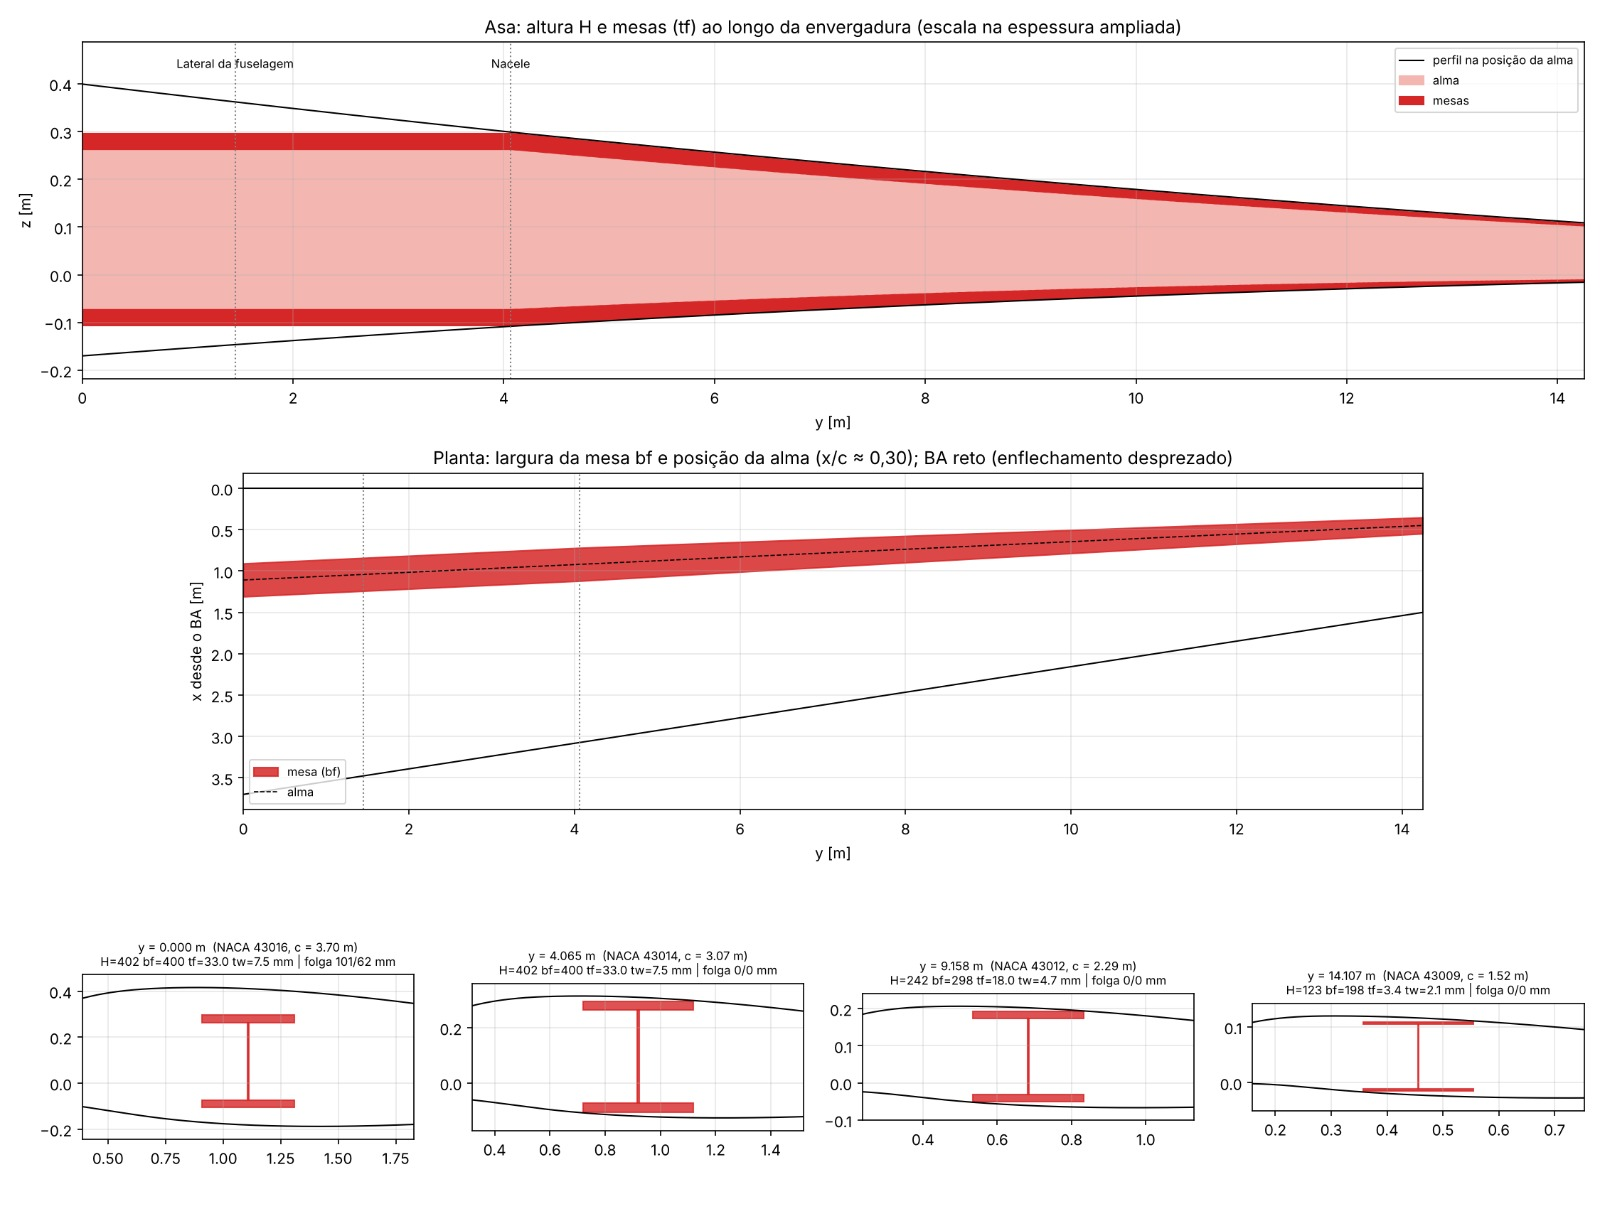
\includegraphics[width=1.0\textwidth]{parte5_longarina.jpeg}
    \caption{Resumo do dimensionamento da longarina ao longo da semienvergadura: elevação (topo), vista em planta (centro) detalhando a posição da alma ($x_{alma}$), evolução geométrica da seção transversal e margens de segurança para os casos de carga críticos (fundo).}
    \label{fig:longarina_resumo}
\end{figure}


\subsection{Nervuras}
\label{sec:nervuras}
De forma preliminar, considera-se 16 nervuras por semiasa, com espaçamento uniforme de 800\,mm a partir da ponta da asa. A seção transversal da alma é retangular, e sua altura útil é governada pela espessura relativa do perfil aerodinâmico na posição $y$ ao longo da envergadura:

\begin{equation}
    h(y) = \frac{t}{c} \cdot c(y)
    \label{eq:altura_alma}
\end{equation}

Adota-se altura efetiva da alma igual a 90\% da altura nominal, a fim de acomodar a espessura das mesas:

\begin{equation}
    h_w = 0{,}9 \cdot h(y)
\end{equation}

Para a seção de raiz, com perfil NACA\,43016 ($t/c = 0{,}16$) e corda $c_\text{raiz} = 3{,}70$\,m:

\begin{equation}
    h_w = 0{,}9 \times 0{,}16 \times 3{,}70 \approx 0{,}53\,\text{m}
\end{equation}

O critério básico de resistência ao cisalhamento impõe:

\begin{equation}
    \tau = \frac{V}{A_w} \leq \tau_\text{adm}
    \label{eq:criterio_cisalhamento}
\end{equation}

\noindent onde $A_w = h_w \cdot t_w$ é a área efetiva da alma e $\tau_\text{adm} = \tau_y / FS$ é a tensão cisalhante admissível. Adotando $\tau_y = 290$\,MPa e fator de segurança $FS = 1{,}5$, conforme requisito FAR\,25.303:

\begin{equation}
    \tau_\text{adm} = \frac{290}{1{,}5} \approx 193\,\text{MPa}
\end{equation}

A força aerodinâmica distribuída absorvida por cada nervura é obtida da derivada da distribuição de força cortante ao longo da envergadura:

\begin{equation}
    F(y) = \left(-\frac{dV}{dy}\right) \cdot \Delta y
    \label{eq:carga_nervura}
\end{equation}

\noindent onde $\Delta y = 800$\,mm é o espaçamento entre nervuras. Dimensionando para a seção de raiz ($y = 0$), região de maior carregamento:

\begin{equation}
    F(0) = 20000\,\frac{\text{N}}{\text{m}} \times 0{,}8\,\text{m}
         = 16000\,\text{N}
\end{equation}

A espessura mínima da alma resulta de:

\begin{equation}
    t_w = \frac{F(0)}{\tau_\text{adm} \cdot h_w}
        = \frac{16000}{193 \times 10^6 \times 0{,}53}
        \approx 1{,}56 \times 10^{-4}\,\text{m}
        = 0{,}156\,\text{mm}
    \label{eq:espessura_minima}
\end{equation}

\noindent Este valor é fisicamente irrealizável, pois é governado pela fabricabilidade mínima de chapas de alumínio. Adota-se, portanto, $t_w = 1{,}0$\,mm.

O resumo dos resultados obtidos estão sintetizados na Tabela \ref{tab:nervuras}, e o arranjo estrutural representado na Figura \ref{fig:cad_dimensionamento_1}.

\begin{table}[H]
\centering
\caption{Parâmetros adotados no dimensionamento preliminar das nervuras.}
\label{tab:nervuras}
\begin{tabular}{lcc}
\toprule
\textbf{Parâmetro} & \textbf{Símbolo} & \textbf{Valor} \\
\midrule
Material                          & ---              & Al\,7075-T6      \\
Nervuras por semiasa              & $n$              & 16               \\
Espaçamento                       & $\Delta y$       & 800\,mm          \\
Altura da alma (raiz)             & $h_w$            & 530\,mm          \\
Espessura mínima adotada          & $t_w$            & 1{,}0\,mm        \\
Tensão cisalhante admissível      & $\tau_\text{adm}$& 193\,MPa         \\
Fator de segurança                & $FS$             & 1{,}5            \\
Carga por nervura (raiz)          & $F(0)$           & 16000\,N      \\
\bottomrule
\end{tabular}
\end{table}

\begin{figure}[H]
    \centering
    % Ajuste o valor 0.8 para 0.7 ou 0.9 dependendo de como ficar no seu PDF
    \caption{Arranjo da longarina e das nervuras da asa.}
    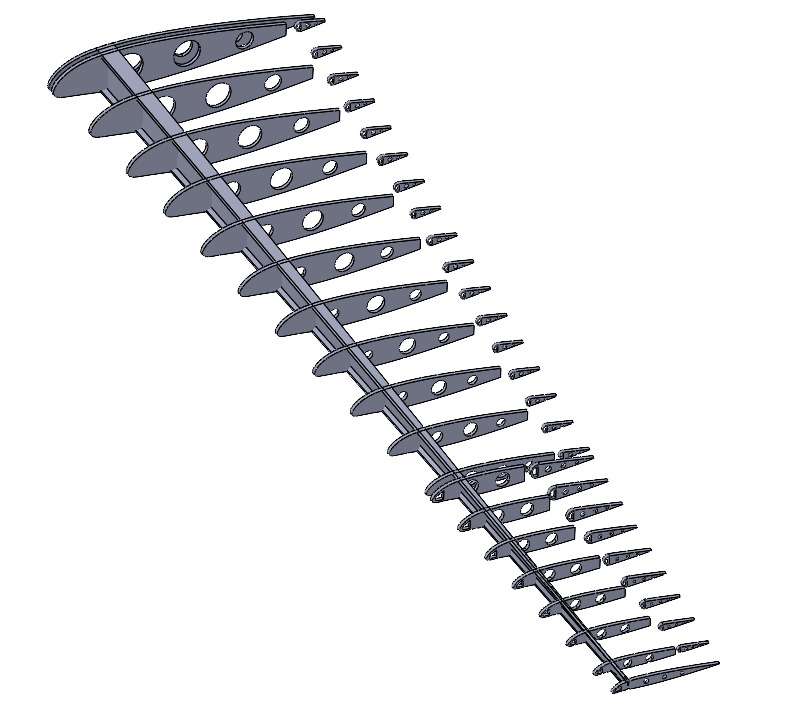
\includegraphics[width=0.6\textwidth]{Images-3-ProjetoDetalhado/cad-01.jpeg}
    \label{fig:cad_dimensionamento_1}
\end{figure}

\subsection{Revestimento}

O revestimento da asa, formado pelo painel e pelos reforçadores longitudinais, foi dimensionado pelo método de Megson \cite{megson2007}. Cada vão entre nervuras é analisado na sua seção interna, que é a mais carregada, e recebe a menor espessura de painel que mantém margem de segurança $MS \ge 0$ em todos os critérios de falha, sob carga última. Os vãos são delimitados pelas nervuras da Seção~\ref{sec:nervuras}, espaçadas de 800\,mm. O primeiro vão vai da lateral da fuselagem ($y = 1{,}45$\,m) até a primeira nervura ($y = 2{,}25$\,m), o que resulta em 16 vãos de 800\,mm por semiasa. A longarina principal é a definida na Seção~\ref{sec:secao_longarina_asa} e faz parte da mesma seção resistente.
 
\subsubsection{Considerações}
 
\begin{itemize}
    \item O diedro e o enflechamento foram desprezados: a linha de 25\% da corda é tomada como reta;
    \item Célula de torção única, em D: o revestimento vai do bordo de ataque até a longarina principal, a 30\% da corda (máxima espessura do perfil), e é fechado pela alma da longarina. O revestimento atrás da longarina é tratado como carenagem e não faz parte da seção resistente;
    \item A longarina principal tem as dimensões $H$, $b_f$, $t_f$ e $t_w$ da Tabela~\ref{tab:longarina_resultados_resumo}, interpoladas linearmente em $y$, e fica centrada na altura local do perfil. A flexão é dividida entre o revestimento e as mesas da longarina, na proporção da rigidez de cada um. A alma da longarina é estendida até o painel para fechar a célula;
    \item A alma da longarina resiste apenas ao cisalhamento;
    \item As cargas foram multiplicadas pelo fator de segurança de 1,5 (\S~25.303 do 14 CFR Part 25). As cargas são apenas aerodinâmicas, sem alívio de inércia do peso da asa, do combustível e do motor;
    \item Painel com reforçadores em Z de espessura igual à do painel ($t_{st} = t_{sk}$), com espaçamento máximo $b_s = 120$\,mm, alma de altura $h_{st} = 60$\,mm e flanges de largura $f_{st} = 0{,}30\,h_{st}$ (Figura~\ref{fig:rev_reforcador});
    \item Espessuras de painéis consideradas: 1,6; 2,0; 2,5; 3,0; 3,5; 4,0; 4,5; 5,0; 5,5; 6,0; 6,5; 7,0; 8,0; 9,0; 10,0; 11,0 e 12,0\,mm;
    \item Propriedades mecânicas conforme seção \ref{tab:propriedades_aluminio_si}.
\end{itemize}

\begin{figure}[H]
    \centering
    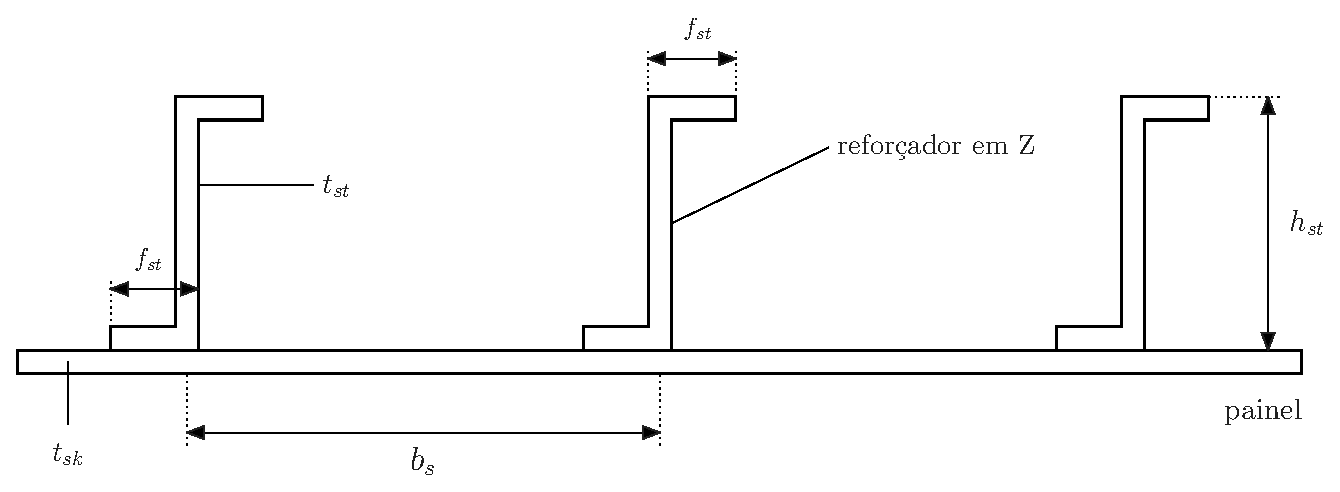
\includegraphics[width=0.9\linewidth]{images/esquema_reforcador.eps}
    \caption{Esquema do painel com reforçadores em Z: altura da alma $h_{st}$, largura das abas $f_{st}$, espessura do reforçador $t_{st}$, espessura do painel $t_{sk}$ e passo $b_s$.}
    \label{fig:rev_reforcador}
\end{figure}
 
\subsubsection{Materiais}
 
Os dois revestimentos trabalham de forma diferente e receberam ligas diferentes (Tabela~\ref{tab:rev_materiais}). O extradorso fica comprimido nas condições de fator de carga positivo, e o que o limita é a flambagem e o escoamento em compressão. Por isso, adotou-se a liga Al\,7075-T6, cuja tensão de escoamento em compressão é 72\% maior que a da liga Al\,2024-T3. O intradorso é tracionado a cada voo, e sua vida é limitada pela fadiga e pela propagação de trincas, que crescem apenas sob tração. Por isso, adotou-se a liga Al\,2024-T3, que tem menor resistência estática, mas maior tenacidade e menor taxa de propagação de trinca. Os reforçadores são de Al\,7075-T6 extrudado.
 
\begin{table}[H]
\centering
\caption{Propriedades dos materiais do revestimento (base A do MIL-HDBK-5, conforme Niu \cite{niu1999})}
\label{tab:rev_materiais}
\small
\begin{tabular}{lccc}
\toprule
 & \makecell{\textbf{Painel do}\\\textbf{extradorso}} & \makecell{\textbf{Painel do}\\\textbf{intradorso}} & \textbf{Reforçadores} \\
\midrule
Liga                                                    & Al\,7075-T6 & Al\,2024-T3 & Al\,7075-T6 \\
Forma                                                   & chapa       & chapa       & extrudado   \\
Escoamento em compressão, $F_{cy}$ [MPa]                & 462         & 269         & 483         \\
Escoamento em tração, $F_{ty}$ [MPa]                    & 476         & 324         & 483         \\
Resistência à tração, $F_{tu}$ [MPa]                    & 524         & 441         & 538         \\
Resistência ao cisalhamento, $F_{su}$ [MPa]             & 296         & 269         & 290         \\
\bottomrule
\end{tabular}
\end{table}
 
\subsubsection{Dados da seção da raiz}
 
As contas a seguir são da seção $y = 1{,}45$\,m, na lateral da fuselagem. Os demais vãos seguem a mesma sequência, e os resultados estão apresentados nas Tabelas~\ref{tab:rev_extradorso} a~\ref{tab:rev_torcao}. A corda local e a espessura relativa são:
 
\begin{equation}
    c(y) = c_{raiz} - (c_{raiz} - c_{ponta})\,\frac{y}{b/2} = 3{,}70 - 2{,}20 \cdot \frac{1{,}45}{14{,}25} = 3{,}476\,\text{m}
    \label{eq:rev_corda}
\end{equation}
 
\begin{equation}
    \frac{t}{c} = 0{,}16 - 0{,}07 \cdot \frac{1{,}45}{14{,}25} = 0{,}153
    \label{eq:rev_tc}
\end{equation}
 
O contorno da célula segue o perfil NACA\,430xx com a espessura relativa da Equação~\ref{eq:rev_tc}, discretizado em 400 pontos por revestimento. A origem fica no eixo de referência das cargas (25\% da corda, sobre a linha da corda), com $x$ para trás, $y$ ao longo da envergadura e $z$ para cima. Na raiz:
 
\begin{itemize}
    \item altura da célula na longarina: $402$\,mm; o bordo de ataque fica $869{,}0$\,mm à frente do eixo de referência;
    \item perímetro do revestimento entre o bordo de ataque e a longarina: $1228{,}4$\,mm no extradorso e $1065{,}7$\,mm no intradorso, o que comporta $n_{st} = 10$ reforçadores no extradorso e $8$ no intradorso, com espaçamentos de $111{,}7$\,mm e $118{,}4$\,mm;
    \item área interna da célula:
    \begin{equation}
        2A_c = \sum_{j} \left(z_j\,x_{j+1} - x_j\,z_{j+1}\right) = 9{,}0553 \times 10^{5}\,\text{mm}^2 \quad\Rightarrow\quad A_c = 452767\,\text{mm}^2
        \label{eq:rev_area}
    \end{equation}
    \item comprimento do vão $\Delta y = 800$\,mm; alma do reforçador $h_{st} = 60$\,mm e flanges $f_{st} = 18$\,mm.
\end{itemize}
 
 
\begin{table}[H]
\centering
\caption{Cargas últimas na seção da raiz ($y = 1{,}45$\,m).}
\label{tab:rev_cargas_raiz}
\begin{tabular}{lccccc}
\toprule
\textbf{Caso} & \makecell{\boldmath$S_z$\\\textbf{[kN]}} & \makecell{\boldmath$M_x$\\\textbf{[kN$\cdot$m]}} & \makecell{\boldmath$M_y$\\\textbf{[kN$\cdot$m]}} & \makecell{\boldmath$S_x$\\\textbf{[kN]}} & \makecell{\boldmath$M_z$\\\textbf{[kN$\cdot$m]}} \\
\midrule
LC4 (manobra, $V_D$, $n_z = 2{,}5$) & $438{,}7$ & $2396$ & $-310{,}4$ & $-19{,}3$ & $104{,}7$ \\
LC5 (manobra, $V_{S,\mathrm{neg}}$, $n_z = -1{,}0$) & $-149{,}6$ & $-817$ & $-66{,}2$ & $-34{,}8$ & $189{,}8$ \\
LC11 (rajada positiva, $V_D$) & $330{,}6$ & $1805$ & $-310{,}4$ & $-4{,}3$ & $23{,}0$ \\
\bottomrule
\end{tabular}
\end{table}
 
\noindent Na Tabela~\ref{tab:rev_cargas_raiz}, $S_z$ é o esforço cortante vertical, $M_x$ o momento fletor, $M_y$ o momento torsor em torno do eixo de referência, $S_x$ o esforço cortante no plano da corda e $M_z$ o momento fletor nesse plano.
 
\subsubsection{Seção idealizada}
 
A seção é idealizada com um \textit{boom} em cada reforçador, um em cada canto da célula (junto à longarina e no bordo de ataque, de cada lado) e um em cada mesa da longarina principal. Cada \textit{boom} de reforçador concentra a área do reforçador e a metade de cada painel vizinho. Nos cantos, o \textit{boom} recebe apenas a metade do painel vizinho. Cada mesa da longarina é um \textit{boom} de área $b_f t_f$, posicionado no centroide da mesa. Os painéis entre \textit{booms} e a alma da longarina resistem apenas a cisalhamento. Para o extradorso da raiz, com painel de $5{,}0$\,mm e espaçamento $b_s = 111{,}7$\,mm, os elementos estão na Tabela~\ref{tab:rev_booms}. A \autoref{fig:rev_secao_celula_D} ilustra a seção idealizada.
 
\begin{table}[H]
\centering
\caption{Composição dos \textit{booms} do extradorso na raiz.}
\label{tab:rev_booms}
\begin{tabular}{lc}
\toprule
\textbf{Elemento} & \textbf{Área [mm$^2$]} \\
\midrule
Aba ligada ao painel $18 \times 5{,}0$                  & $90$ \\
Alma $60 \times 5{,}0$                                 & $300$ \\
Aba livre $18 \times 5{,}0$                            & $90$ \\
\midrule
Reforçador, $A_{st}$                                    & $480$ \\
Painel, $b_s \times t_{sk} = 111{,}7 \times 5{,}0$      & $558{,}4$ \\
\midrule
\textit{Boom} de reforçador, $B_{st} = A_{st} + b_s t_{sk}$     & $1038{,}4$ \\
\textit{Boom} de canto, $B_{c} = b_s t_{sk}/2$                  & $279{,}2$ \\
\textit{Boom} da mesa da longarina, $b_f t_f = 400 \times 33$ & $13200$ \\
\bottomrule
\end{tabular}
\end{table}
 
\noindent Para o intradorso, com painel de $7{,}0$\,mm e espaçamento de $118{,}4$\,mm: $A_{st} = 672$\,mm$^2$, $B_{st} = 1500{,}9$\,mm$^2$ e $B_c = 414{,}4$\,mm$^2$. A seção da raiz tem, portanto, $24$ \textit{booms} ($10$ reforçadores e 2 cantos no extradorso, $8$ reforçadores e 2 cantos no intradorso e as 2 mesas da longarina), ligados por $20$ painéis e pela alma da longarina.
 
\noindent A espessura equivalente, $t_{eq} = \sum B / s$, é a de uma chapa com a mesma área dos \textit{booms} de um revestimento de perímetro $s$, sem as mesas da longarina: na raiz, $8{,}91$\,mm no extradorso e $12{,}04$\,mm no intradorso. Ela é usada apenas para apresentar os resultados e calcular a massa.

\begin{figure}[H]
    \centering
    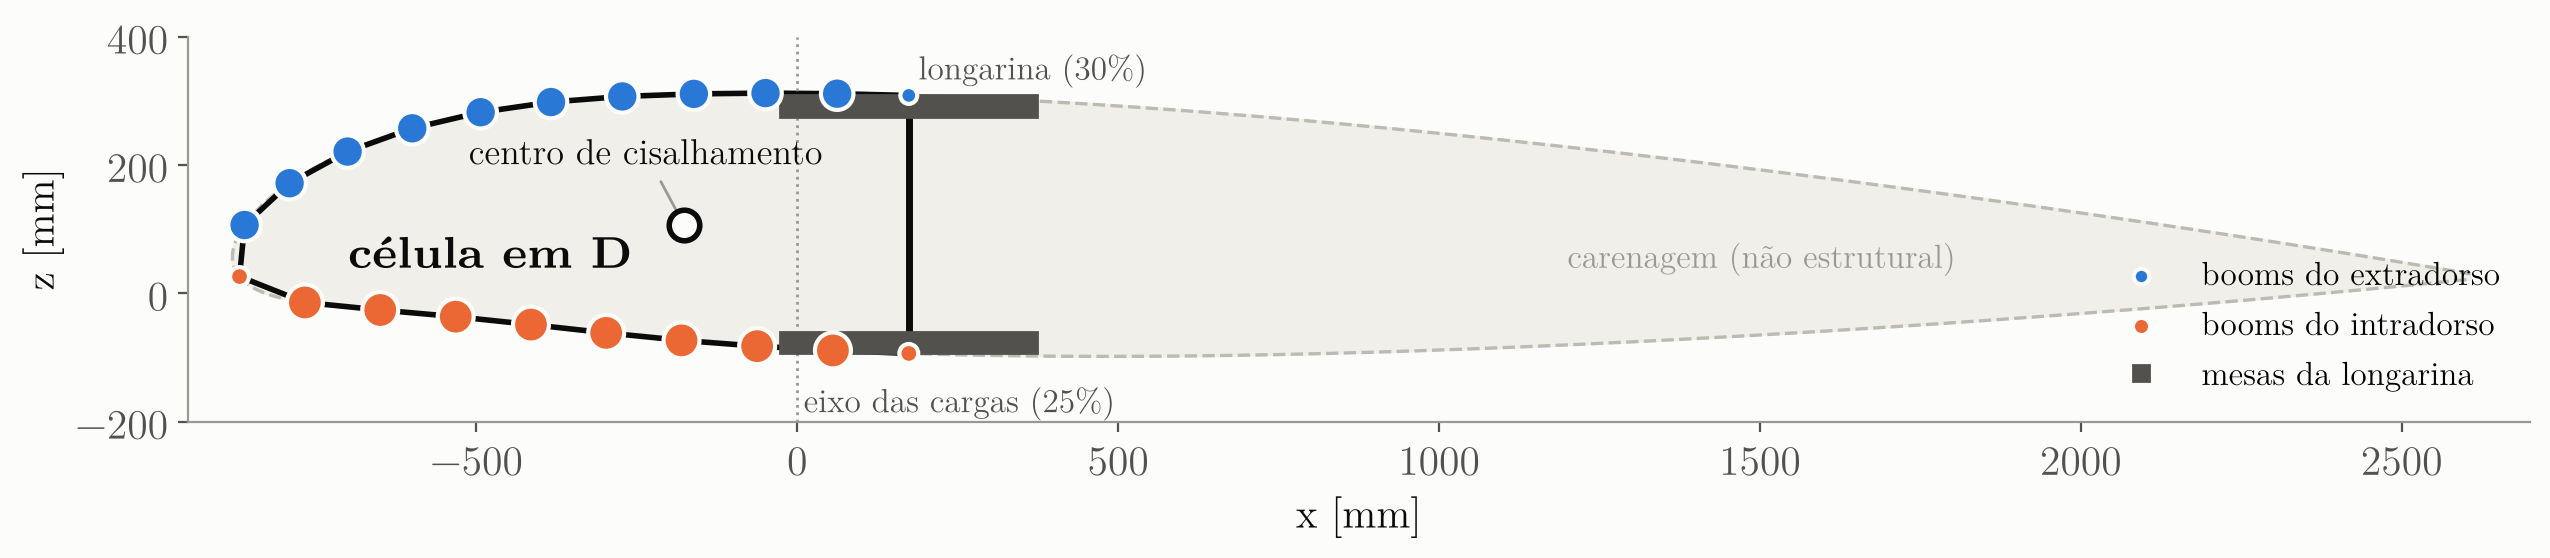
\includegraphics[width=1\linewidth]{1_secao_celula_D.png}
    \caption{Esquema da seção resistente da asa na raiz: célula em D, formada pelo painel do bordo de ataque e pela alma da longarina principal.}
    \label{fig:rev_secao_celula_D}
\end{figure}
 
\subsubsection{Tensão normal}
 
A tensão normal de flexão pode ser definida por:
 
\begin{equation}
    \sigma = a_x\,x + a_z\,z, \qquad
    a_x = \frac{M_z I_{xx} + M_x I_{xz}}{D}, \qquad
    a_z = -\frac{M_x I_{zz} + M_z I_{xz}}{D}
    \label{eq:rev_sigma}
\end{equation}

sendo,

\begin{equation}
    D = I_{xx} I_{zz} - I_{xz}^2 = 1{,}2254 \times 10^{19}\,\text{mm}^8
    \label{eq:rev_D}
\end{equation}
 
Para o caso LC4, com $M_x = 2{,}396 \times 10^{9}$\,N$\cdot$mm e $M_z = 1{,}047 \times 10^{8}$\,N$\cdot$mm, resultam $a_x = 0{,}05042$\,MPa/mm e $a_z = -1{,}2011$\,MPa/mm. No ponto mais comprimido do extradorso ($x = -69{,}8$\,mm e $z = 281{,}3$\,mm, em relação ao centroide):
 
\begin{equation}
    \sigma = -3{,}5 + (-337{,}9) = -341{,}4\,\text{MPa}
    \label{eq:rev_sigma_max}
\end{equation}
 
A Tabela~\ref{tab:rev_tensoes_raiz} resume as tensões máximas dos três casos.
 
\begin{table}[H]
\centering
\caption{Tensões normais últimas na raiz.}
\label{tab:rev_tensoes_raiz}
\begin{tabular}{lcccc}
\toprule
\textbf{Caso} & \makecell{\textbf{Extradorso}\\\textbf{[MPa]}} & \makecell{\textbf{Intradorso}\\\textbf{[MPa]}} & \makecell{\textbf{Mesa superior}\\\textbf{[MPa]}} & \makecell{\textbf{Mesa inferior}\\\textbf{[MPa]}} \\
\midrule
LC4 & $-341{,}4$ & $318{,}4$ & $-222{,}8$ & $220{,}4$ \\
LC5 & $118{,}3$ & $-98{,}0$ & $85{,}1$ & $-64{,}9$ \\
LC11 & $-256{,}4$ & $237{,}3$ & $-170{,}1$ & $163{,}6$ \\
\bottomrule
\end{tabular}
\end{table}
 
\subsubsection{Fluxo de cisalhamento}
 
Como a asa afila ao longo da envergadura, os \textit{booms} são inclinados, e a componente vertical da sua carga resiste a parte do cortante. Para o caso LC4, somando extradorso, intradorso e mesas da longarina:
 
\begin{equation}
    P_z = \sigma B \frac{\mathrm{d}z}{\mathrm{d}y}, \qquad
    \sum P_z = 63{,}1 + 35{,}2 + 0{,}2 = 98{,}5\,\text{kN}
    \label{eq:rev_Pz}
\end{equation}
 
\begin{equation}
    \begin{gathered}
        S_{z,w} = S_z - \sum P_z = 438{,}7 - 98{,}5 = 340{,}2\,\text{kN} \\
        S_{x,w} = S_x - \sum P_x = -19{,}25 - (-9{,}64) = -9{,}61\,\text{kN}
    \end{gathered}
    \label{eq:rev_Sw}
\end{equation}
 
A seção é cortada no primeiro painel do extradorso, e o fluxo da seção aberta é acumulado \textit{boom} a \textit{boom}, assim, conforme Megson:
 
\begin{equation}
    q_{b,r} = q_{b,r-1} - \left[\frac{S_{x,w} I_{xx} - S_{z,w} I_{xz}}{D}\, x_r + \frac{S_{z,w} I_{zz} - S_{x,w} I_{xz}}{D}\, z_r\right] B_r
    \label{eq:rev_qb}
\end{equation}
 
O fluxo constante que fecha a seção vem do equilíbrio de momentos em torno do eixo de referência das cargas (Eq.~(17.17) do Megson), em que $p$ é o braço de cada painel em relação a esse eixo e $\sum p\,\mathrm{d}s = 2A_c$:
 
\begin{equation}
    \begin{aligned}
        q_{s,0} &= \frac{M_y - \sum (z P_x - x P_z) - \sum q_b\, p\, \mathrm{d}s}{2A_c} \\
        &= \frac{\left[-310{,}4 + (-15{,}2) + 176{,}3\right] \times 10^{6}}{0{,}9055 \times 10^{6}} = -164{,}8\,\text{N/mm}
    \end{aligned}
    \label{eq:rev_qs0}
\end{equation}
 
O fluxo total é $q = q_b + q_{s,0}$. No extradorso, ele varia de $-165$\,N/mm junto ao bordo de ataque a $-560$\,N/mm junto à longarina. Na alma da longarina, entre as mesas, o fluxo é $-993{,}4$\,N/mm: como as mesas são \textit{booms} de grande área, é nesse trecho que a longarina leva a maior parte do cortante vertical. As tensões de cisalhamento máximas são:
 
\begin{equation}
    \begin{gathered}
        \tau_{extr} = \frac{560{,}3}{5{,}0} = 112{,}1\,\text{MPa}, \qquad
        \tau_{intr} = \frac{564{,}8}{7{,}0} = 80{,}7\,\text{MPa} \\
        \tau_{w} = \frac{993{,}4}{7{,}0} = 141{,}9\,\text{MPa}
    \end{gathered}
    \label{eq:rev_tau}
\end{equation}
 
\noindent em que $\tau_w$ é a tensão na alma da longarina.
 
\begin{table}[H]
\centering
\caption{Cisalhamento último na seção da raiz.}
\label{tab:rev_cisalhamento_raiz}
\begin{tabular}{lccccc}
\toprule
\textbf{Caso} & \makecell{\boldmath$S_{z,w}$\\\textbf{[kN]}} & \makecell{\boldmath$q_{s,0}$\\\textbf{[N/mm]}} & \makecell{\boldmath$\tau_{extr}$\\\textbf{[MPa]}} & \makecell{\boldmath$\tau_{intr}$\\\textbf{[MPa]}} & \makecell{\boldmath$\tau_{w}$\\\textbf{[MPa]}} \\
\midrule
LC4 & $340{,}2$ & $-164{,}8$ & $112{,}1$ & $80{,}7$ & $141{,}9$ \\
LC5 & $-115{,}9$ & $-128{,}5$ & $26{,}0$ & $17{,}6$ & $21{,}8$ \\
LC11 & $256{,}3$ & $-210{,}0$ & $100{,}7$ & $73{,}7$ & $119{,}1$ \\
\bottomrule
\end{tabular}
\end{table}
 
\subsubsection{Centro de cisalhamento e torção}
 
O equilíbrio de momentos da Equação~\ref{eq:rev_qs0} resolve cortante e torção em conjunto. Para separar as duas parcelas, calcula-se o centro de cisalhamento (CC), transfere-se a carga para ele e trata-se o momento resultante como torção pura. Nesta parte, a correção de afilamento não é aplicada. As paredes que resistem ao cisalhamento são os painéis e a alma da longarina:
 
\begin{equation}
    \oint \frac{\mathrm{d}s}{t} = \frac{1228{,}4}{5{,}0} + \frac{1065{,}7}{7{,}0} + \frac{402}{7{,}0} = 245{,}7 + 152{,}2 + 76{,}0 = 473{,}9
    \label{eq:rev_dst}
\end{equation}
 
Aplicando uma força unitária $S_z = 1$\,N, calcula-se o fluxo da seção aberta pela Equação~\ref{eq:rev_qb} e fecha-se a seção pela condição de giro nulo (Eq.~(17.27) do Megson):
 
\begin{equation}
    q_{s,0} = -\frac{\oint (q_b/t)\,\mathrm{d}s}{\oint \mathrm{d}s/t} = -\frac{-0{,}3569}{473{,}9} = 7{,}530 \times 10^{-4}\,\text{N/mm por N}
    \label{eq:rev_qs0_cc}
\end{equation}
 
O momento desse fluxo em torno do eixo de referência é igual ao da força aplicada no centro de cisalhamento, $-x_{cc} S_z$:
 
\begin{equation}
    \begin{aligned}
        \sum q\,p\,\mathrm{d}s &= \sum q_b\,p\,\mathrm{d}s + q_{s,0}\,(2A_c) \\
        &= -513{,}9 + \left(7{,}530 \times 10^{-4}\right)\left(9{,}0553 \times 10^{5}\right) = 167{,}9\,\text{N}\cdot\text{mm}
    \end{aligned}
    \label{eq:rev_xcc}
\end{equation}
 
Portanto, $x_{cc} = -167{,}9$\,mm: o centro de cisalhamento fica $167{,}9$\,mm à frente do eixo de referência, ou seja, a $0{,}25 - 167{,}9/3476 = 0{,}202$ da corda ($20{,}2$\%). Repetindo o cálculo com $S_x = 1$\,N, obtém-se $\sum q_b\,p\,\mathrm{d}s = 152{,}6$\,N$\cdot$mm e $q_{s,0} = -7{,}886 \times 10^{-5}$\,N/mm, de onde $z_{cc} = 81{,}2$\,mm acima da linha da corda. O momento torsor em torno do centro de cisalhamento é:
 
\begin{equation}
    T = M_y + x_{cc} S_z - z_{cc} S_x
    \label{eq:rev_T}
\end{equation}
 
\noindent O primeiro termo é o momento de arfagem das cargas; o segundo vem da sustentação, que atua cerca de $5$\% da corda atrás do centro de cisalhamento e, por isso, também tende a baixar o nariz; o terceiro vem da força no plano da corda (Tabela~\ref{tab:rev_torque_raiz}).
 
\begin{table}[H]
\centering
\caption{Momento torsor último em torno do centro de cisalhamento, na raiz.}
\label{tab:rev_torque_raiz}
\begin{tabular}{lcccc}
\toprule
\textbf{Caso} & \makecell{\boldmath$M_y$\\\textbf{[kN$\cdot$m]}} & \makecell{\boldmath$x_{cc} S_z$\\\textbf{[kN$\cdot$m]}} & \makecell{\boldmath$-z_{cc} S_x$\\\textbf{[kN$\cdot$m]}} & \makecell{\boldmath$T$\\\textbf{[kN$\cdot$m]}} \\
\midrule
LC4 & $-310{,}4$ & $-73{,}7$ & $1{,}6$ & $-382{,}5$ \\
LC5 & $-66{,}2$ & $25{,}1$ & $2{,}8$ & $-38{,}3$ \\
LC11 & $-310{,}4$ & $-55{,}5$ & $0{,}4$ & $-365{,}5$ \\
\bottomrule
\end{tabular}
\end{table}
 
O caso crítico em torção é o LC4: com o centro de cisalhamento à frente do eixo das cargas, a sustentação soma-se ao momento de arfagem, e o LC4 é o caso de maior sustentação. O fluxo de torção pura, segundo Megson, é definido por:
 
\begin{equation}
    q_T = \frac{T}{2A_c} = \frac{-382{,}5 \times 10^{6}}{9{,}0553 \times 10^{5}} = -422{,}4\,\text{N/mm}
    \label{eq:rev_qT}
\end{equation}
 
\noindent o que corresponde a $84{,}5$\,MPa no painel do extradorso, $60{,}3$\,MPa no do intradorso, $60{,}3$\,MPa na alma da longarina. A rigidez torcional da célula é:
 
\begin{equation}
    J = \frac{(2A_c)^2}{\oint \mathrm{d}s/t} = 1{,}730 \times 10^{9}\,\text{mm}^4, \qquad GJ = 4{,}671 \times 10^{13}\,\text{N}\cdot\text{mm}^2 = 46{,}7\,\text{MN}\cdot\text{m}^2
    \label{eq:rev_J}
\end{equation}
 
A taxa de giro é calculada com o momento torsor limite, igual ao último dividido por 1,5. Para o caso LC4, na raiz:
 
\begin{equation}
    \frac{\mathrm{d}\theta}{\mathrm{d}y} = \frac{T/1{,}5}{GJ} = \frac{-255{,}0 \times 10^{6}}{4{,}671 \times 10^{13}} = -5{,}458 \times 10^{-6}\,\text{rad/mm} = -0{,}3127\,^\circ\text{/m}
    \label{eq:rev_dtheta}
\end{equation}
 
O giro é integrado a partir da nervura da raiz, considerada engastada, com momento torsor nulo na ponta:
 
\begin{equation}
    \theta_{i+1} = \theta_i + \frac{1}{2}\left(\theta'_i + \theta'_{i+1}\right) \Delta y_i
    \label{eq:rev_theta}
\end{equation}
 
\noindent No primeiro vão, $\theta_2 = \tfrac{1}{2}\left[-0{,}3127 + (-0{,}3598)\right] \times 0{,}8 = -0{,}269^\circ$. Os demais vãos estão na Tabela~\ref{tab:rev_torcao}.
 
\subsubsection{Resultados por vão}
 
As Tabelas~\ref{tab:rev_extradorso} e~\ref{tab:rev_intradorso} apresentam o painel escolhido em cada vão. Nelas, $y$ é a posição da seção interna do vão, $h_{st}$ a altura da alma do reforçador, $n_{st}$ o número de reforçadores entre o bordo de ataque e a longarina e $t_{eq}$ a espessura equivalente (soma das áreas dos \textit{booms} dividida pelo perímetro); a espessura do reforçador é igual à do painel. As tensões são últimas e máximas entre os três casos de carga.
 
\begin{table}[H]
\centering
\caption{Painel do extradorso (Al\,7075-T6) em cada vão.}
\label{tab:rev_extradorso}
\small
\setlength{\tabcolsep}{4pt}
\begin{tabular}{ccccccccc}
\toprule
\textbf{Vão} & \makecell{\boldmath$y$\\\textbf{[m]}} & \makecell{\boldmath$h_{st}$\\\textbf{[mm]}} & \makecell{\boldmath$t_{sk}$\\\textbf{[mm]}} & \boldmath$n_{st}$ & \makecell{\boldmath$t_{eq}$\\\textbf{[mm]}} & \makecell{\boldmath$\sigma_c$\\\textbf{[MPa]}} & \makecell{\boldmath$\sigma_t$\\\textbf{[MPa]}} & \makecell{\boldmath$\tau$\\\textbf{[MPa]}} \\
\midrule
1 & 1{,}45 & 60{,}0 & 5{,}0 & 10 & 8{,}91 & 341 & 118 & 112{,}1 \\
2 & 2{,}25 & 60{,}0 & 4{,}5 & 9 & 7{,}80 & 323 & 114 & 115{,}2 \\
3 & 3{,}05 & 60{,}0 & 4{,}5 & 9 & 7{,}94 & 280 & 153 & 106{,}9 \\
4 & 3{,}85 & 60{,}0 & 4{,}0 & 9 & 7{,}19 & 243 & 146 & 107{,}8 \\
5 & 4{,}65 & 60{,}0 & 4{,}0 & 8 & 6{,}96 & 228 & 134 & 91{,}0 \\
6 & 5{,}45 & 60{,}0 & 4{,}0 & 8 & 7{,}11 & 218 & 132 & 88{,}9 \\
7 & 6{,}25 & 60{,}0 & 4{,}0 & 7 & 6{,}85 & 211 & 132 & 85{,}8 \\
8 & 7{,}05 & 60{,}0 & 3{,}5 & 7 & 6{,}12 & 206 & 119 & 92{,}7 \\
9 & 7{,}85 & 60{,}0 & 3{,}5 & 7 & 6{,}27 & 189 & 113 & 90{,}2 \\
10 & 8{,}65 & 60{,}0 & 3{,}5 & 6 & 6{,}01 & 173 & 108 & 84{,}4 \\
11 & 9{,}45 & 56{,}1 & 3{,}5 & 6 & 5{,}98 & 150 & 96 & 79{,}9 \\
12 & 10{,}25 & 51{,}1 & 3{,}0 & 5 & 4{,}72 & 138 & 73 & 81{,}0 \\
13 & 11{,}05 & 46{,}4 & 3{,}0 & 5 & 4{,}66 & 107 & 71 & 71{,}7 \\
14 & 11{,}85 & 41{,}9 & 2{,}5 & 5 & 3{,}84 & 80 & 50 & 69{,}7 \\
15 & 12{,}65 & 37{,}7 & 2{,}0 & 4 & 2{,}83 & 50 & 24 & 61{,}9 \\
16 & 13{,}45 & 33{,}6 & 1{,}6 & 4 & 2{,}24 & 17 & 8 & 42{,}7 \\
\bottomrule
\end{tabular}
\end{table}
 
\begin{table}[H]
\centering
\caption{Painel do intradorso (Al\,2024-T3) em cada vão.}
\label{tab:rev_intradorso}
\small
\setlength{\tabcolsep}{4pt}
\begin{tabular}{ccccccccc}
\toprule
\textbf{Vão} & \makecell{\boldmath$y$\\\textbf{[m]}} & \makecell{\boldmath$h_{st}$\\\textbf{[mm]}} & \makecell{\boldmath$t_{sk}$\\\textbf{[mm]}} & \boldmath$n_{st}$ & \makecell{\boldmath$t_{eq}$\\\textbf{[mm]}} & \makecell{\boldmath$\sigma_c$\\\textbf{[MPa]}} & \makecell{\boldmath$\sigma_t$\\\textbf{[MPa]}} & \makecell{\boldmath$\tau$\\\textbf{[MPa]}} \\
\midrule
1 & 1{,}45 & 60{,}0 & 7{,}0 & 8 & 12{,}04 & 98 & 318 & 80{,}7 \\
2 & 2{,}25 & 60{,}0 & 5{,}0 & 8 & 8{,}74 & 99 & 317 & 100{,}7 \\
3 & 3{,}05 & 60{,}0 & 3{,}0 & 8 & 5{,}33 & 102 & 304 & 141{,}3 \\
4 & 3{,}85 & 60{,}0 & 2{,}5 & 7 & 4{,}27 & 98 & 267 & 148{,}7 \\
5 & 4{,}65 & 60{,}0 & 2{,}5 & 7 & 4{,}35 & 90 & 248 & 129{,}0 \\
6 & 5{,}45 & 60{,}0 & 2{,}5 & 7 & 4{,}43 & 85 & 239 & 125{,}5 \\
7 & 6{,}25 & 60{,}0 & 2{,}5 & 6 & 4{,}23 & 82 & 232 & 120{,}5 \\
8 & 7{,}05 & 60{,}0 & 2{,}5 & 6 & 4{,}31 & 75 & 221 & 115{,}8 \\
9 & 7{,}85 & 60{,}0 & 2{,}5 & 6 & 4{,}41 & 68 & 204 & 112{,}2 \\
10 & 8{,}65 & 60{,}0 & 2{,}5 & 5 & 4{,}17 & 61 & 188 & 104{,}5 \\
11 & 9{,}45 & 56{,}1 & 2{,}5 & 5 & 4{,}15 & 53 & 165 & 98{,}5 \\
12 & 10{,}25 & 51{,}1 & 2{,}5 & 5 & 4{,}09 & 45 & 142 & 89{,}1 \\
13 & 11{,}05 & 46{,}4 & 2{,}0 & 5 & 3{,}23 & 37 & 118 & 95{,}1 \\
14 & 11{,}85 & 41{,}9 & 2{,}0 & 4 & 2{,}95 & 27 & 86 & 77{,}4 \\
15 & 12{,}65 & 37{,}7 & 2{,}0 & 4 & 2{,}91 & 16 & 49 & 58{,}0 \\
16 & 13{,}45 & 33{,}6 & 1{,}6 & 4 & 2{,}30 & 5 & 16 & 40{,}1 \\
\bottomrule
\end{tabular}
\end{table}

As margens de segurança estão na Tabela~\ref{tab:rev_ms}. Cada valor é o menor entre os três casos de carga.
 
\begin{table}[H]
\centering
\caption{Margens de segurança do painel em cada vão (mínimo entre os três casos de carga).}
\label{tab:rev_ms}
\small
\setlength{\tabcolsep}{4pt}
\begin{tabular}{ccccc}
\toprule
 & \multicolumn{2}{c}{\textbf{Extradorso}} & \multicolumn{2}{c}{\textbf{Intradorso}} \\
\cmidrule(lr){2-3}\cmidrule(lr){4-5}
\textbf{Vão} & \textbf{Cisalhamento} & \textbf{Tração} & \textbf{Cisalhamento} & \textbf{Tração} \\
\midrule
1 & 1{,}57 & 3{,}12 & 0{,}81 & 0{,}01 \\
2 & 1{,}52 & 3{,}33 & 0{,}54 & 0{,}04 \\
3 & 1{,}50 & 2{,}12 & 0{,}10 & 0{,}06 \\
4 & 1{,}70 & 2{,}54 & 0{,}20 & 0{,}27 \\
5 & 1{,}93 & 2{,}55 & 0{,}16 & 0{,}31 \\
6 & 2{,}00 & 2{,}60 & 0{,}19 & 0{,}36 \\
7 & 2{,}11 & 2{,}60 & 0{,}24 & 0{,}40 \\
8 & 2{,}20 & 2{,}74 & 0{,}28 & 0{,}49 \\
9 & 1{,}96 & 3{,}22 & 0{,}33 & 0{,}59 \\
10 & 2{,}16 & 3{,}42 & 0{,}43 & 0{,}72 \\
11 & 2{,}34 & 3{,}94 & 0{,}51 & 0{,}96 \\
12 & 1{,}65 & $>5$ & 0{,}67 & 1{,}27 \\
13 & 1{,}99 & $>5$ & 0{,}003 & 1{,}75 \\
14 & 1{,}14 & $>5$ & 0{,}23 & 2{,}78 \\
15 & 1{,}88 & $>5$ & 0{,}63 & $>5$ \\
16 & 0{,}43 & $>5$ & 0{,}52 & $>5$ \\
\bottomrule
\end{tabular}
\end{table}
 
A Tabela~\ref{tab:rev_torcao} apresenta a posição do centro de cisalhamento, a rigidez torcional, o momento torsor último, o cisalhamento na alma da longarina e o giro na carga limite ao longo da semiasa.
 
\begin{table}[H]
\centering
\caption{Centro de cisalhamento (CC), rigidez torcional, momento torsor último, cisalhamento na alma da longarina e giro na carga limite.}
\label{tab:rev_torcao}
\small
\setlength{\tabcolsep}{3.5pt}
\begin{tabular}{ccccccccccc}
\toprule
 & & \textbf{CC} & \boldmath$z_{cc}$ & \boldmath$GJ$ & \multicolumn{3}{c}{\boldmath$T$ \textbf{[kN$\cdot$m]}} & \boldmath$\tau_w$ & \multicolumn{2}{c}{\textbf{Giro [$^\circ$]}} \\
\cmidrule(lr){6-8}\cmidrule(lr){10-11}
\textbf{Vão} & \boldmath$y$ \textbf{[m]} & \textbf{[\% corda]} & \textbf{[mm]} & \textbf{[MN$\cdot$m$^2$]} & \textbf{LC4} & \textbf{LC5} & \textbf{LC11} & \textbf{[MPa]} & \textbf{LC4} & \textbf{LC11} \\
\midrule
1 & 1{,}45 & 20{,}2 & 81{,}2 & 46{,}7 & $-382{,}5$ & $-38{,}3$ & $-365{,}5$ & 141{,}9 & $0{,}00$ & $0{,}00$ \\
2 & 2{,}25 & 21{,}6 & 112{,}3 & 33{,}7 & $-317{,}9$ & $-38{,}9$ & $-307{,}9$ & 144{,}9 & $-0{,}27$ & $-0{,}26$ \\
3 & 3{,}05 & 23{,}1 & 179{,}3 & 22{,}9 & $-257{,}6$ & $-37{,}6$ & $-254{,}2$ & 144{,}4 & $-0{,}58$ & $-0{,}57$ \\
4 & 3{,}85 & 24{,}1 & 178{,}6 & 16{,}9 & $-211{,}7$ & $-35{,}8$ & $-211{,}4$ & 140{,}2 & $-0{,}95$ & $-0{,}93$ \\
5 & 4{,}65 & 24{,}0 & 171{,}2 & 14{,}1 & $-182{,}1$ & $-30{,}4$ & $-181{,}7$ & 110{,}2 & $-1{,}34$ & $-1{,}32$ \\
6 & 5{,}45 & 23{,}8 & 162{,}9 & 11{,}7 & $-156{,}6$ & $-25{,}2$ & $-155{,}8$ & 112{,}0 & $-1{,}74$ & $-1{,}72$ \\
7 & 6{,}25 & 23{,}5 & 154{,}4 & 9{,}7 & $-133{,}1$ & $-20{,}7$ & $-132{,}0$ & 115{,}8 & $-2{,}15$ & $-2{,}13$ \\
8 & 7{,}05 & 23{,}6 & 133{,}6 & 7{,}5 & $-110{,}7$ & $-17{,}5$ & $-109{,}7$ & 117{,}4 & $-2{,}59$ & $-2{,}56$ \\
9 & 7{,}85 & 23{,}2 & 126{,}6 & 6{,}1 & $-92{,}1$ & $-13{,}8$ & $-91{,}0$ & 119{,}6 & $-3{,}05$ & $-3{,}01$ \\
10 & 8{,}65 & 22{,}9 & 119{,}4 & 4{,}9 & $-75{,}2$ & $-10{,}8$ & $-74{,}0$ & 119{,}6 & $-3{,}52$ & $-3{,}48$ \\
11 & 9{,}45 & 22{,}5 & 112{,}6 & 3{,}9 & $-60{,}2$ & $-8{,}2$ & $-59{,}0$ & 119{,}6 & $-3{,}99$ & $-3{,}94$ \\
12 & 10{,}25 & 22{,}5 & 96{,}4 & 2{,}8 & $-45{,}9$ & $-6{,}5$ & $-45{,}0$ & 116{,}6 & $-4{,}48$ & $-4{,}42$ \\
13 & 11{,}05 & 22{,}5 & 104{,}8 & 2{,}0 & $-33{,}4$ & $-4{,}7$ & $-32{,}8$ & 110{,}7 & $-4{,}98$ & $-4{,}92$ \\
14 & 11{,}85 & 22{,}5 & 86{,}6 & 1{,}4 & $-22{,}9$ & $-3{,}4$ & $-22{,}5$ & 99{,}0 & $-5{,}50$ & $-5{,}42$ \\
15 & 12{,}65 & 22{,}5 & 70{,}2 & 0{,}9 & $-13{,}9$ & $-2{,}1$ & $-13{,}6$ & 79{,}4 & $-5{,}97$ & $-5{,}89$ \\
16 & 13{,}45 & 22{,}6 & 65{,}7 & 0{,}6 & $-6{,}3$ & $-1{,}0$ & $-6{,}2$ & 47{,}3 & $-6{,}37$ & $-6{,}28$ \\
\midrule
ponta & 14{,}25 & -- & -- & -- & $0$ & $0$ & $0$ & -- & $-6{,}54$ & $-6{,}45$ \\
\bottomrule
\end{tabular}
\end{table}
 
\subsubsection{Resumo dos resultados}
 
A Tabela~\ref{tab:rev_resumo} reúne os principais resultados do revestimento.
 
\begin{table}[H]
\centering
\caption{Resumo do dimensionamento do revestimento da asa.}
\label{tab:rev_resumo}
\begin{tabular}{lcc}
\toprule
\textbf{Grandeza} & \textbf{Raiz} (\boldmath$y = 1{,}45$ \textbf{m}) & \textbf{Último vão} \\
\midrule
Painel do extradorso                      & $5{,}0$\,mm                     & $1{,}6$\,mm \\
Painel do intradorso                      & $7{,}0$\,mm                     & $1{,}6$\,mm \\
Espessura equivalente do extradorso     & $8{,}91$\,mm                  & $2{,}24$\,mm \\
Espessura equivalente do intradorso     & $12{,}04$\,mm                  & $2{,}30$\,mm \\
Reforçadores (extradorso / intradorso)  & $10$ / $8$             & $4$ / $4$ \\
Altura da alma do reforçador            & $60$\,mm                       & $33{,}6$\,mm \\
Compressão última no extradorso         & $341{,}4$\,MPa                & $16{,}9$\,MPa \\
Tração última no intradorso             & $318{,}4$\,MPa                & $16{,}5$\,MPa \\
Parcela de $M_x$ levada pela longarina (LC4) & $45$\%              & $50$\% \\
Centro de cisalhamento                  & $20{,}2$\% da corda             & $22{,}6$\% da corda \\
Rigidez torcional $GJ$                  & $46{,}7$\,MN$\cdot$m$^2$         & $0{,}6$\,MN$\cdot$m$^2$ \\
Momento torsor último (LC4)            & $-382{,}5$\,kN$\cdot$m              & -- \\
Giro na carga limite (LC4)              & 0 (engaste)                     & $-6{,}54^\circ$ na ponta \\
\bottomrule
\end{tabular}
\end{table}

\subsection{Análise de Flambagem}

Para a análise de flambagem da asa, será adotado inicialmente um painel do extradorso próximo à raiz, entre duas nervuras e dois reforçadores consecutivos. Considera-se a largura $b_s=120\ mm$ como o espaçamento entre reforçadores, a espessura para o extradorso em 5,5 mm, para o intradorso de 6,0 mm e o comprimento longitudinal $a = 800\ mm$. Considerando ainda os materiais conforme a Tabela \ref{tab:rev_materiais}, a equação de flambagem para a chapa isolada será: 

\begin{equation}
    \sigma_{\mathrm{cr,sk}} =
\frac{k_c \pi^2 E}{12(1-\nu^2)}
\left(\frac{t}{b_s}\right)^2
\end{equation}
Em que o coeficiente de flambagem k, pelas condições de contorno e considerando placa longa $(a/b_s = 6,875)$, pode ser estimado pelos ábacos de \textit{Megson}  como \cite{megson2007}: 

\begin{equation}
    k_c \approx 4
\end{equation}


Para avaliação da flambagem por cisalhamento, utiliza-se a equação:

\begin{equation}
    \tau_{\mathrm{cr,sk}} =
\frac{k_s \pi^2 E}{12(1-\nu^2)}
\left(\frac{t}{b_s}\right)^2
\end{equation}

Em que o coeficiente k pode novamente ser avaliado via ábaco de forma que:

\begin{equation}
    k_s \approx 5{,}34 + \frac{4}{(a/b_s)^2}\approx 5,42
\end{equation}

Com isso, chega-se a:

\begin{equation}
    \sigma_{cr,sk}\approx 539 \ MPa
\end{equation}

\begin{equation}
    \tau_{cr,sk}\approx 731 \ MPa
\end{equation}


Ademais, as razões de carregamento compressivo e cisalhante em relação às cargas últimas podem ser definidas como:

\begin{equation}
    R_c = \frac{|\sigma|}{\sigma_{\mathrm{cr}}}
\end{equation}

\begin{equation}
    R_s = \frac{|\tau|}{\tau_{\mathrm{cr}}}
\end{equation}

Portanto, com base nos carregamentos atuantes expostos nas Tabelas \ref{tab:rev_tensoes_raiz} e \ref{tab:rev_cisalhamento_raiz}, a Tabela \ref{tab:razoes_utilizacao_extradorso} reúne os resultados para as taxas de carregamento para as diferentes condições.

\begin{table}[H]
    \centering
    \caption{Razões de utilização do extradorso}
    \label{tab:razoes_utilizacao_extradorso}
    \begin{tabular}{|c|c|c|c|}
        \hline
        \textbf{Caso de carga} &
        \textbf{$R_c$} &
        \textbf{$R_s$} &
        \textbf{$R_c+R_s$} \\
        \hline
        LC4  & $0{,}625$ & $0{,}091$ & $0{,}716$ \\
        \hline
        LC5  & $0{,}000$ & $0{,}039$ & $0{,}039$ \\
        \hline
        LC11 & $0{,}467$ & $0{,}081$ & $0{,}548$ \\
        \hline
    \end{tabular}
\end{table}


Dessa forma, percebe-se que, mesmo considerando os carregamentos aplicados com um  fator de segurança de 1,5, os carregamentos atuantes não alcançam os limites, e seu efeito combinado estimado pela soma das razões também permanece acomodado dentro do limite.

Analisando o perfil Z, pode-se avaliar a flambagem na alma conforme a expressão:


\begin{equation}
    \sigma_{\mathrm{cr,web}} =
\frac{k_c \pi^2 E}{12(1-\nu^2)}
\left(\frac{5,5}{60}\right)^2
\end{equation}

O que leva a:

\begin{equation}
    \sigma_{\mathrm{cr,web}} =
2150\  MPa
\end{equation}


Para as flanges, considerando largura de 18 mm e espessura de 5,5 mm, o fator k pode ser estimado em torno de 0,4. Com isso, conclui-se que:

\begin{equation}
    \sigma_{\mathrm{cr,flange}} \approx
2570\  MPa
\end{equation}

Nota-se, então, que as tensões críticas na alma e nas flanges do reforçador superam bastante os carregamentos atuantes.

Para a análise do conjunto painel-reforçador, a equação a seguir pode ser adotada, assumindo-se condições de contorno de apoio simples (consideração esta que é razoável para a situação):

\begin{equation}
    F_{cr}\approx 3,60E\left(\frac{t}{b_s}\right)^2
\end{equation}

Como o extradorso possui a menor espessura e, portanto, possuirá o menor valor de $F_{cr}$, a equação será avaliada para ele, o que resulta em:

\begin{equation}
    F_{cr}\approx 537\ MPa
\end{equation}

Com isso, é verificada uma grande proximidade entre os resultados dessa aproximação e o valor calculado pela equação completa para o revestimento.

É necessário, ainda, verificar a ocorrência de falha local no reforçador em Z. Para tal, será utilizado o método de Gerard. A falha local consiste na perda de capacidade resistente de uma região específica de um componente estrutural, sem que seja necessário ocorrer, inicialmente, a instabilidade ou a falha do componente como um todo. Pelo método de Gerard, ela é estimada para um reforçador em Z por meio de:

\begin{equation}
    \frac{F_{cs}}{F_{cy}}=3,2\left[\frac{t^2}{A}\left(\frac{E}{F_{cy}}\right)^{1/3}\right]^{0,75}
\end{equation}

Em que $F_{cy}$ é o limite de escoamento do material e A é a área do perfil. Considerando uma área estimada em $528\ mm²$, e um limite de escoamento de 483 MPa, obtém-se pelo método de Gerard:

\begin{equation}
    F_{cs}= 351 \ MPa
\end{equation}

\begin{equation}
    \frac{F_{cs}}{F_{cy}}= 0,73
\end{equation}

De acordo com \textit{Megson}, o limite máximo para a razão $\frac{F_{cs}}{F_{cy}}$ deve ser de 0,9. Logo, para o reforçador proposto, a condição é atendida \cite{megson2007}.

Em síntese, os resultados obtidos indicam que o dimensionamento preliminar do revestimento e dos reforçadores da asa atende aos critérios de flambagem considerados. Para o painel do extradorso, a maior razão de utilização combinada foi de 0,716, correspondente ao caso de carga LC4, permanecendo abaixo do limite admissível. 

De forma semelhante, as tensões críticas calculadas para a alma e as flanges do reforçador em Z superam os carregamentos atuantes, indicando margem em relação à flambagem local desses elementos. A análise do conjunto painel-reforçador também apresentou resultados consistentes com os obtidos para a chapa isolada, enquanto a avaliação pelo método de Gerard resultou em uma razão \(F_{cs}/F_{cy}=0,73\), inferior ao limite de 0,9 recomendado por Megson. Portanto, considerando as hipóteses adotadas e os modos de falha avaliados, a configuração estrutural proposta apresenta comportamento satisfatório quanto à estabilidade sob compressão e cisalhamento.

Ressalta-se, contudo, que essa conclusão se restringe às regiões, aos casos de carga e aos mecanismos de falha analisados, sendo recomendável complementar a avaliação com verificações adicionais de estabilidade global e validação dos resultados à medida que o projeto estrutural for refinado.

\section{Empenagem Horizontal}
\subsection{Longarina da EH}

O dimensionamento da longarina da empenagem horizontal (EH) adota a mesma metodologia estrutural e os mesmos critérios de falha descritos para a seção da asa \ref{sec:secao_longarina_asa}. 

O material empregado permanece a liga de alumínio 7075-T6. A análise estrutural avalia os esforços atuantes decorrentes de três casos de carga críticos específicos para a superfície horizontal: LC41, LC10 e LC42.

A geometria da longarina apresenta uma seção transversal constante da raiz até a junção com o cone de cauda, localizada na estação $y = 0,50$ m. A partir desse ponto até a ponta da semienvergadura, as dimensões da seção afilam linearmente, com a altura estrutural máxima limitada pela geometria do perfil aerodinâmico NACA 0012 local.   A otimização geométrica do trecho constante resultou em uma seção com altura $H = 314$ mm, largura de mesa $b_f = 50$ mm, espessura de mesa $t_f = 5,5$ mm e espessura de alma $t_w = 6,0$ mm. Na estação da ponta, a seção atinge as dimensões mínimas de $H = 196$ mm, $b_f = 50$ mm, $t_f = 3,0$ mm e $t_w = 2,0$ mm, suficientes para manter as margens de segurança positivas. A massa estrutural total computada para a longarina completa da EH (abrangendo as duas semienvergaduras) é de $36,7$ kg.

A tabela \ref{tab:longarina_eh_resultados} resume os valores das dimensões da longarina da EH em cada seção da mesma.

\begin{table}[H]
    \centering
    \caption{Distribuição das dimensões geométricas da longarina da EH e massa linear ao longo da semienvergadura.}
    \vspace{0.2cm}
    \begin{tabular}{cccccccc}
        \hline
        \textbf{$y$ [m]} & \textbf{Corda [m]} & \textbf{Perfil} & \textbf{$H$ [mm]} & \textbf{$b_f$ [mm]} & \textbf{$t_f$ [mm]} & \textbf{$t_w$ [mm]} & \textbf{Massa [kg/m]} \\
        \hline
        0,000 & 2,788 & NACA 0012 & 314 & 50,0 & 5,50 & 6,00 & 6,65 \\
        0,500 & 2,655 & NACA 0012 & 314 & 50,0 & 5,50 & 6,00 & 6,65 \\
        1,250 & 2,455 & NACA 0012 & 290 & 50,0 & 4,99 & 5,19 & 5,48 \\
        2,000 & 2,255 & NACA 0012 & 266 & 50,0 & 4,48 & 4,37 & 4,42 \\
        2,750 & 2,056 & NACA 0012 & 242 & 50,0 & 3,97 & 3,56 & 3,46 \\
        3,500 & 1,856 & NACA 0012 & 218 & 50,0 & 3,47 & 2,75 & 2,60 \\
        4,188 & 1,673 & NACA 0012 & 196 & 50,0 & 3,00 & 2,00 & 1,91 \\
        \hline
    \end{tabular}
    \label{tab:longarina_eh_resultados}
\end{table}

Na figura \ref{fig:longarina_EH_resumo}, são resumidas e apresentadas as dimensões da longarina ao longo da asa, bem como as margens de segurança e as folgas em algumas seções relevantes da asa.

\begin{figure}[H]
    \centering
    % Ajuste \textwidth para um tamanho menor se a imagem ficar grande demais
    % ou use \linewidth.
    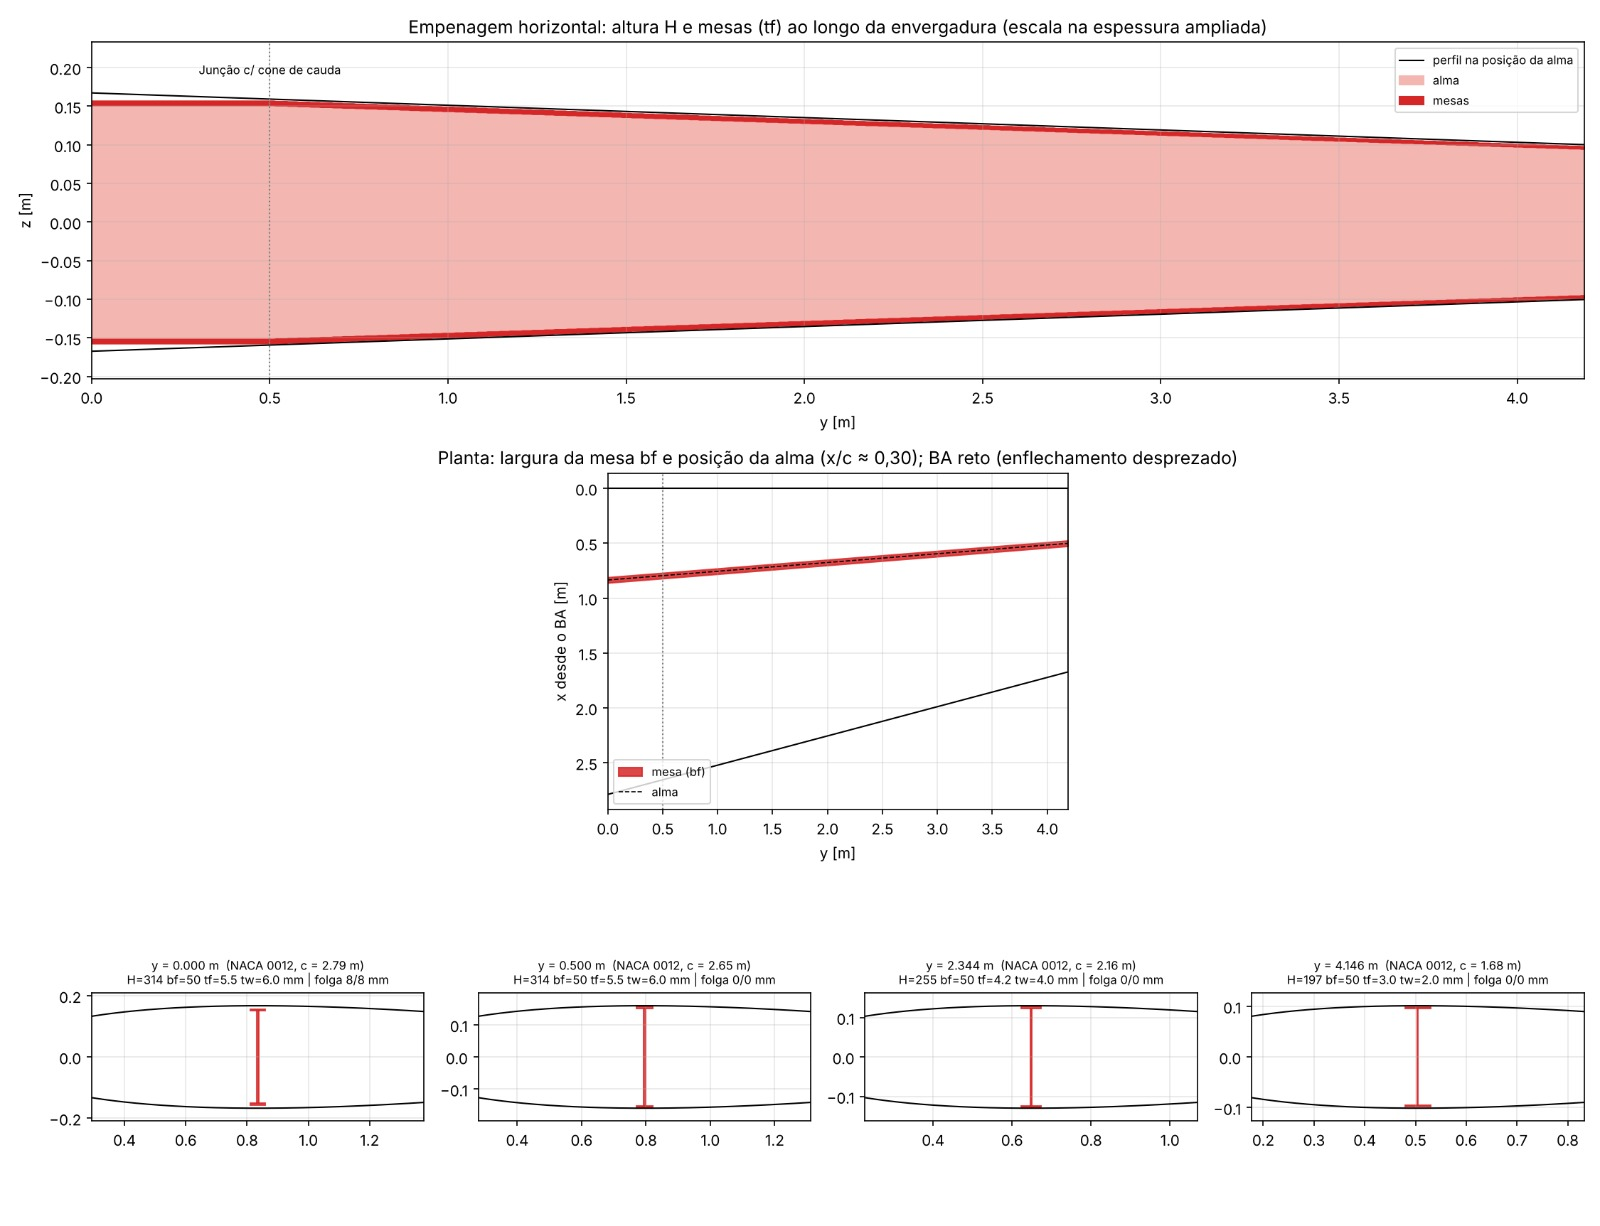
\includegraphics[width=1.0\textwidth]{eh_parte5_longarina.jpeg}
    \caption{Resumo do dimensionamento da longarina ao longo da semienvergadura: elevação (topo), vista em planta (centro) detalhando a posição da alma ($x_{alma}$), evolução geométrica da seção transversal e margens de segurança para os casos de carga críticos (fundo).}
    \label{fig:longarina_EH_resumo}
\end{figure}

\section{Empenagem Vertical}
\subsection{Longarina da EV}

O dimensionamento da longarina da empenagem vertical (EV) adota a mesma metodologia estrutural e os mesmos critérios de falha descritos para a seção da asa \ref{sec:secao_longarina_asa}. 

O material empregado permanece a liga de alumínio 7075-T6. A análise estrutural avalia os esforços atuantes decorrentes de dois casos de carga críticos específicos para a superfície vertical: LC63 e LC61.

A geometria da longarina apresenta uma seção transversal constante da base até a junção com a fuselagem, localizada na estação vertical $z = 0,335$ m. A partir desse ponto até a ponta da superfície, as dimensões da seção afilam linearmente, com a altura estrutural máxima limitada pela geometria do perfil aerodinâmico NACA 0012 local. A otimização geométrica do trecho constante resultou em uma seção com altura $H = 477$ mm, largura de mesa $b_f = 50$ mm, espessura de mesa $t_f = 3,5$ mm e espessura de alma $t_w = 7,0$ mm. Na estação da ponta, a seção atinge as dimensões mínimas de $H = 245$ mm, $b_f = 50$ mm, $t_f = 3,0$ mm e $t_w = 2,0$ mm, suficientes para manter as margens de segurança positivas. A massa estrutural total computada para a longarina completa da EV (uma única superfície) é de $29,4$ kg.

A tabela \ref{tab:longarina_ev_resultados} resume os valores das dimensões da longarina da EV em cada seção da mesma.

\begin{table}[H]
    \centering
    \caption{Distribuição das dimensões geométricas da longarina da EV e massa linear ao longo da altura.}
    \vspace{0.2cm}
    \begin{tabular}{cccccccc}
        \hline
        \textbf{$z$ [m]} & \textbf{Corda [m]} & \textbf{Perfil} & \textbf{$H$ [mm]} & \textbf{$b_f$ [mm]} & \textbf{$t_f$ [mm]} & \textbf{$t_w$ [mm]} & \textbf{Massa [kg/m]} \\
        \hline
        0,000 & 4,158 & NACA 0012 & 477 & 50,0 & 3,50 & 7,00 & 10,23 \\
        0,335 & 4,017 & NACA 0012 & 477 & 50,0 & 3,50 & 7,00 & 10,23 \\
        1,000 & 3,736 & NACA 0012 & 444 & 50,0 & 3,43 & 6,28 & 8,67 \\
        2,000 & 3,311 & NACA 0012 & 393 & 50,0 & 3,32 & 5,19 & 6,64 \\
        3,000 & 2,890 & NACA 0012 & 342 & 50,0 & 3,21 & 4,10 & 4,81 \\
        4,000 & 2,469 & NACA 0012 & 292 & 50,0 & 3,10 & 3,01 & 3,29 \\
        4,925 & 2,079 & NACA 0012 & 245 & 50,0 & 3,00 & 2,00 & 2,19 \\
        \hline
    \end{tabular}
    \label{tab:longarina_ev_resultados}
\end{table}

Na figura \ref{fig:longarina_EV_resumo}, são resumidas e apresentadas as dimensões da longarina ao longo da altura, bem como as margens de segurança e as folgas em algumas seções relevantes da EV.

\begin{figure}[H]
    \centering
    % Ajuste \textwidth para um tamanho menor se a imagem ficar grande demais
    % ou use \linewidth.
    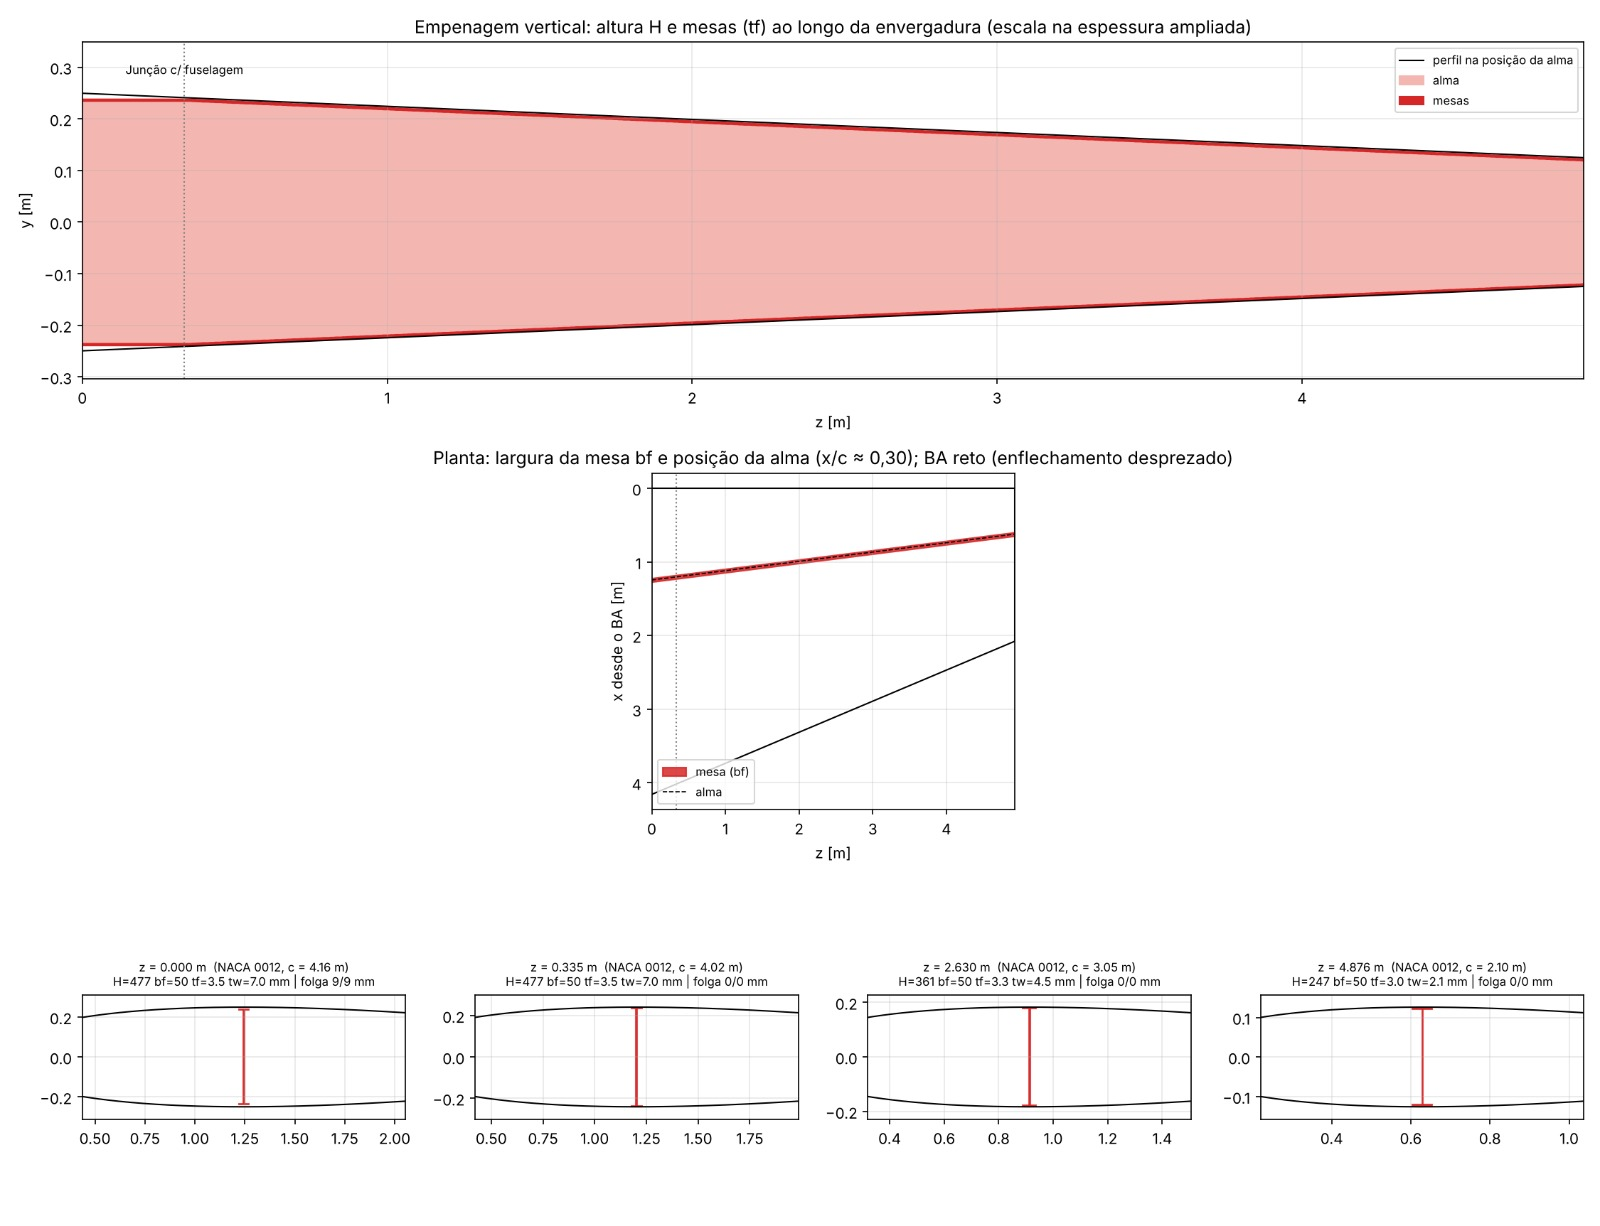
\includegraphics[width=1.0\textwidth]{ev_parte5_longarina.jpeg}
    \caption{Resumo do dimensionamento da longarina ao longo da altura da EV: elevação (topo), vista em planta (centro) detalhando a posição da alma ($x_{alma}$), evolução geométrica da seção transversal e margens de segurança para os casos de carga críticos (fundo).}
    \label{fig:longarina_EV_resumo}
\end{figure}

\section{Resumo das longarinas}

A tabela \ref{tab:resumo_longarinas} a seguir resume o dimensionamento das longarinas da Asa, da EH e da EV da aeronave, servindo como base para comparação entre elas e como cálculo preliminar do peso estrutural adicionado.

\begin{table}[H]
    \centering
    \caption{Resumo geral do dimensionamento das longarinas (Massa computada para a longarina inteira: asa e EH = duas metades, EV = uma).}
    \vspace{0.2cm}
    \resizebox{\textwidth}{!}{
    \begin{tabular}{lcccc}
        \hline
        \textbf{Superfície} & \textbf{Raiz: $H \times b_f \times t_f \times t_w$ [mm]} & \textbf{Ponta: $H \times b_f \times t_f \times t_w$ [mm]} & \textbf{Massa [kg]} & \textbf{MS mín (critério, caso)} \\
        \hline
        Asa & $402 \times 400 \times 33,0 \times 7,5$ & $120 \times 195 \times 3,0 \times 2,0$ & 1395,9 & $+0,006$ (resistência, LC4) \\
        Empenagem horizontal & $314 \times 50 \times 5,5 \times 6,0$ & $196 \times 50 \times 3,0 \times 2,0$ & 36,7 & $+0,038$ (resistência, LC10) \\
        Empenagem vertical & $477 \times 50 \times 3,5 \times 7,0$ & $245 \times 50 \times 3,0 \times 2,0$ & 29,4 & $+0,053$ (flambagem da alma, LC63) \\
        \hline
        \textbf{Total} & & & \textbf{1462,0} & \\
        \hline
    \end{tabular}
    }
    \label{tab:resumo_longarinas}
\end{table}

\begin{figure}[H]
    \centering
    \caption{Arranjo estrutural das empenagens.}
    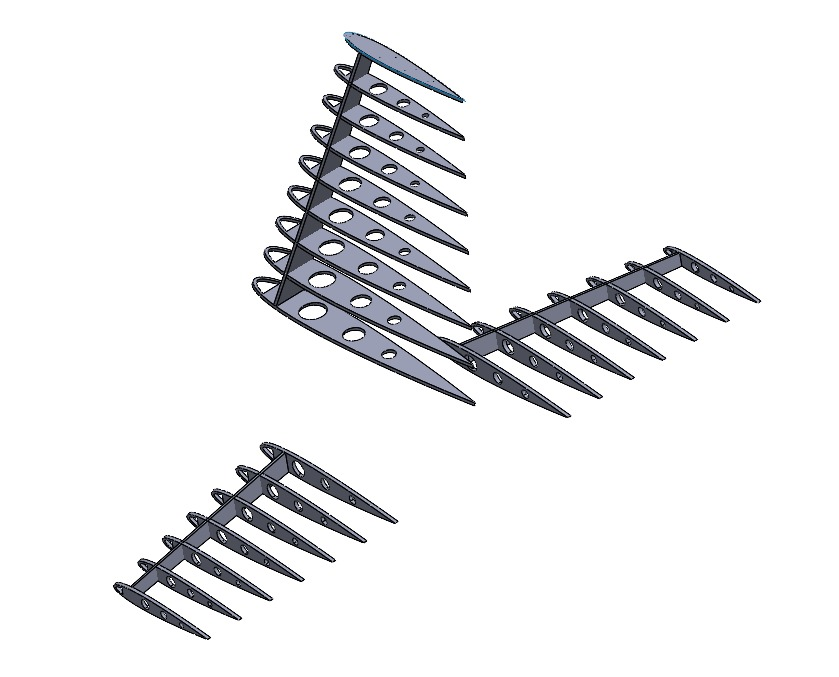
\includegraphics[width=0.6\textwidth]{Images-3-ProjetoDetalhado/cad-02.jpeg}
    \label{fig:cad_dimensionamento_2}
\end{figure}

\section{Fuselagem}
\label{sec:fuselagem}

A fuselagem foi dimensionada como uma casca semi-monocoque idealizada: cilindro de raio $R = 1{,}45$~m e comprimento $\ell = 16{,}0$~m, composta por revestimento, reforçadores longitudinais (\textit{stringers}) em Z e cavernas de seção retangular. A seção foi mantida constante.Adotou-se material único, liga Al 2024-T3 conforme propriedades da Tabela \ref{tab:propriedades_aluminio_si}.
 
A torção na fuselagem, constante entre a empenagem e a asa, foi tomada como o maior valor entre a contribuição da EV e a da EH:
\begin{equation}
  T_{EV} = M_{f,EV} + F_{EV}\, z_{EV}, \qquad
  T_{EH} = (1 - 0{,}8)\, M_{f,EH},
\end{equation}
com $M_{f}$ o fletor de raiz e $z_{EV}$ a altura da raiz da EV em relação ao eixo da fuselagem.
 
As condições consideradas são as críticas das empenagens: LC10 e LC41 (Tabela \ref{tab:cargas_criticas_eh}), e LC61 e LC63 (Tabela \ref{tab:cargas_criticas_ev}). As forças na direção $x$ das superfícies foram desprezadas por serem uma ordem de grandeza inferiores às forças em $z$ (EH) e em $y$ (EV).
 
O dimensionamento usa o envelope dos máximos ao longo do eixo longitudinal e entre condições, aplicados simultaneamente, o que é conservativo:
\begin{equation}
  M_u = FS\sqrt{M_{y,\max}^2 + M_{z,\max}^2}, \quad
  V_u = FS\sqrt{V_{z,\max}^2 + V_{y,\max}^2}, \quad
  T_u = FS \cdot T_{\max}, \qquad FS = 1{,}5 .
\end{equation}
% O trecho entre as longarinas foi excluído do envelope. Nesse trecho, o apoio em dois pontos produz um pico de cortante associado ao binário das reações, típico da região de transferência de carga, que pertence ao dimensionamento detalhado.
 
Como a massa da casca entra nas cargas de inércia, o cálculo é iterativo. Parte-se de uma estimativa de ($3000$~kg). Dimensiona-se, e a massa obtida realimenta as cargas até que a variação seja inferior a 1\%. A convergência ocorreu em 3 iterações.
 
\subsection{Critérios de dimensionamento}
 
As propriedades da seção usam a espessura equivalente $t_{eq} = t + A_s/b$ para tensões longitudinais, onde $A_s$ é a área de um reforçador e $b = 2\pi R/n_s$ o espaçamento entre reforçadores. Para cisalhamento e tensão circunferencial, considera-se apenas o revestimento. Na posição angular $\theta$ (medida a partir do ponto de flexão máxima):
\begin{equation}
  \sigma_x(\theta) = \frac{M_u}{\pi R^2 t_{eq}}\cos\theta + \frac{\Delta p_u R}{2\, t_{eq}}, \quad
  \sigma_\theta = \frac{\Delta p_u R}{t}, \quad
  \tau(\theta) = \frac{1}{t}\left(\frac{T_u}{2\pi R^2} + \frac{V_u}{\pi R}\sin\theta\right).
\end{equation}
 
Cada critério abaixo exige margem de segurança mínima $MS = F_{adm}/f - 1 \geq \pend{0{,}10}$, calculada na carga última.
 
\begin{enumerate}
  \item \textbf{Resistência do revestimento} (von Mises), varrendo $\theta \in [0,\pi]$, com e sem pressurização ($\Delta p_u = 1{,}5\,\Delta p$ e $\Delta p_u = 0$):
  \begin{equation}
    \sigma_{vm} = \sqrt{\sigma_x^2 - \sigma_x\sigma_\theta + \sigma_\theta^2 + 3\tau^2} \leq F_{tu}.
  \end{equation}
  \item \textbf{Pressão isolada} (FAR 25.365(d)): $1{,}33\,\Delta p$ como carga limite, com $\sigma_\theta \leq F_{ty}$ na limite e $\sigma_\theta \leq F_{tu}$ na última.
  \item \textbf{Compressão no reforçador}, sem pressurização: $\sigma_{st} = M_u/(\pi R^2 t_{eq}) \leq F_{cy}$.
  \item \textbf{Flambagem do painel} $b \times L$, sem pressurização, por interação compressão--cisalhamento de placa plana (a curvatura foi desprezada, o que é conservativo), com o revestimento sem flambar até $\pend{FS_{pan}}$ vezes a carga limite:
  \begin{equation}
    \begin{aligned}
      \sigma_{cr} &= k_c\frac{\pi^2 E}{12(1-\nu^2)}\left(\frac{t}{b}\right)^2, & \quad k_c &= \min_m\left(\frac{m b}{L} + \frac{L}{m b}\right)^2, \\[1ex]
      \tau_{cr} &= k_s\frac{\pi^2 E}{12(1-\nu^2)}\left(\frac{t}{b}\right)^2, & \quad k_s &= 5{,}35 + 4\left(\frac{b}{L}\right)^2,
    \end{aligned}
  \end{equation}
  \begin{equation}
    R_c + R_s^2 \leq 1, \qquad R_c = \sigma_c/\sigma_{cr}, \quad R_s = \tau/\tau_{cr},
  \end{equation}
  com $\sigma_{cr} \leq F_{cy}$ e $\tau_{cr} \leq F_{ty}/\sqrt{3}$ como cortes de plasticidade.
  
  \item \textbf{Coluna do reforçador} entre cavernas (reforçador mais a faixa de revestimento colaborante $b_e$), biapoiada, com comprimento efetivo $L$. Usa-se Euler para $L/\rho \geq \sqrt{2\pi^2E/F_{cy}}$ e Johnson caso contrário:
  \begin{equation}
    \sigma_{cr} = \frac{\pi^2 E}{(L/\rho)^2}
    \quad\text{ou}\quad
    \sigma_{cr} = F_{cy} - \frac{F_{cy}^2}{4\pi^2 E}\left(\frac{L}{\rho}\right)^2,
    \qquad \rho = \sqrt{I_{col}/A_{col}} .
  \end{equation}
  % O \textit{crippling} local foi substituído pela restrição geométrica $h_s/t_s \leq 30$, com flanges do Z iguais a $0{,}4\,h_s$.
  \item \textbf{Cavernas} pelo critério de rigidez de Shanley, para evitar instabilidade geral:
  \begin{equation}
    (EI)_{f} \geq (1 + MS)\, C_f\frac{M_u D^2}{L}, \qquad C_f = \frac{1}{16000}.
  \end{equation}
  Para a seção retangular $h \times w$, a massa por rigidez decresce com $h$, então a altura é definida pelas restrições adotadas: $h \leq \pend{100}$~mm, $h/w \leq 15$ e $w \geq \pend{1{,}5}$~mm.
\end{enumerate}
 
\subsection{Otimização}
 
O problema consiste em minimizar a massa da casca,
\begin{equation}
  m = \rho\,\ell\,\left(2\pi R\,t + n_s A_s\right) + n_f\,\rho\, h w\, 2\pi\!\left(R - \tfrac{h}{2}\right), \qquad n_f = \left\lfloor \ell/L \right\rfloor + 1,
\end{equation}
sujeito a todos os critérios da seção anterior. Foi feita uma busca exaustiva sobre um espaço discreto de projeto:
 
\begin{itemize}
  \item espessura do revestimento $t$: bitolas comerciais de 0,81 a 6,35~mm (15 valores);
  \item espessura do reforçador $t_s$: bitolas de 0,81 a 4,06~mm (10 valores);
  \item altura do reforçador $h_s$: 15 a 60~mm, espaçamento de 2,5~mm;
  \item número de reforçadores $n_s$: 40 a 240, múltiplos de 4, com espaçamento mínimo $b \geq \pend{100}$~mm (restrição de fabricação);
  \item espaçamento das cavernas $L$: 300 a 800~mm, espaçamento de 50~mm.
\end{itemize}
 
Para cada par $(L, n_s)$, todas as combinações $(t, t_s, h_s)$ são avaliadas simultaneamente. A caverna é dimensionada diretamente pelo critério de Shanley, pois depende apenas de $L$. A solução é a combinação viável de menor massa. Como o espaço é discreto e totalmente varrido, o mínimo obtido é global dentro do espaço considerado, sem dependência de ponto inicial. A verificação de que a solução não está na fronteira do espaço de busca confirma que o espaço foi suficiente. Esse laço de otimização fica dentro do laço de peso próprio.
 
\subsection{Resultados}
 
\begin{table}[H]
  \centering
  \caption{Esforços de envelope da fuselagem.}
  \begin{tabular}{lcc}
    \toprule
    Esforço & Limite & Último \\
    \midrule
    $M_{y,\max}$ ($x = 9{,}76$~m) [kN$\cdot$m] & 528,3 & -- \\
    $M_{z,\max}$ [kN$\cdot$m]                 & 293,1 & -- \\
    $M$ resultante [kN$\cdot$m]               & --    & 906,3 \\
    $V_{z,\max}$ / $V_{y,\max}$ [kN]          & 50,6 / 36,5 & -- \\
    $V$ resultante [kN]                       & --    & 93,6 \\
    $T_{\max}$ [kN$\cdot$m]                   & 108,1 & 162,2 \\
    \bottomrule
  \end{tabular}
\end{table}
 
As reações da asa sobre a fuselagem, obtidas por equilíbrio, foram de $-14{,}2$~kN (LC10) e $129{,}8$~kN (LC41).
 
\begin{table}[H]
  \centering
  \caption{Configuração de menor massa.}
  \begin{tabular}{llr}
    \toprule
    Componente & Parâmetro & Valor \\
    \midrule
    Revestimento      & espessura $t$ [mm]                   & 1,80 \\
    Reforçador & quantidade $n_s$ / espaçamento $b$ [mm]    & 88 / 103,5 \\
              & seção Z: $h_s \times t_s$, aba [mm]  & $22{,}5 \times 0{,}81$, 9,0 \\
              & área $A_s$ [mm$^2$]                  & 32,8 \\
              & esbeltez da coluna $L/\rho$          & 98,9 \\
    Cavernas  & espaçamento $L$ [mm] / quantidade    & 550 / 30 \\
              & seção retangular $h \times w$ [mm]   & $39{,}2 \times 2{,}62$ \\
              & $I$ / $I_{\text{Shanley}}$ [m$^4$]   & $1{,}316\times10^{-8}$ / $1{,}196\times10^{-8}$ \\
    \midrule
    Massa     & revestimento / reforçadores / cavernas [kg]     & \pend{729,2 / 128,4 / 77,0} \\
              & \textbf{total da casca} [kg]         & \textbf{934,7} \\
    \bottomrule
  \end{tabular}
\end{table}
 
A espessura do revestimento resultou governada pelos critérios de flexão e estabilidade, e não pela pressurização. A seção da caverna ficou limitada pela razão $h/w$ imposta, de modo que sua altura reflete essa restrição e não um ótimo estrutural. O reforçador resultou na menor bitola disponível ($t_s = 0{,}81$~mm), que corresponde ao limite inferior de fabricação adotado.
 
O envelope simultâneo de $M$, $V$ e $T$ e a seção constante tornam o resultado conservativo em massa. A seção constante obriga regiões menos solicitadas, como o nariz e cone de cauda, a usar a mesma seção da região crítica, junto à asa. Um zoneamento da espessura reduziria a massa.

A Figura \ref{fig:cad_dimensionamento_3} representa o arranjo estrutural final dos componentes críticos da aeronave.

\begin{figure}[H]
    \centering
    \caption{Arranjo estrutural da aeronave completa.}
    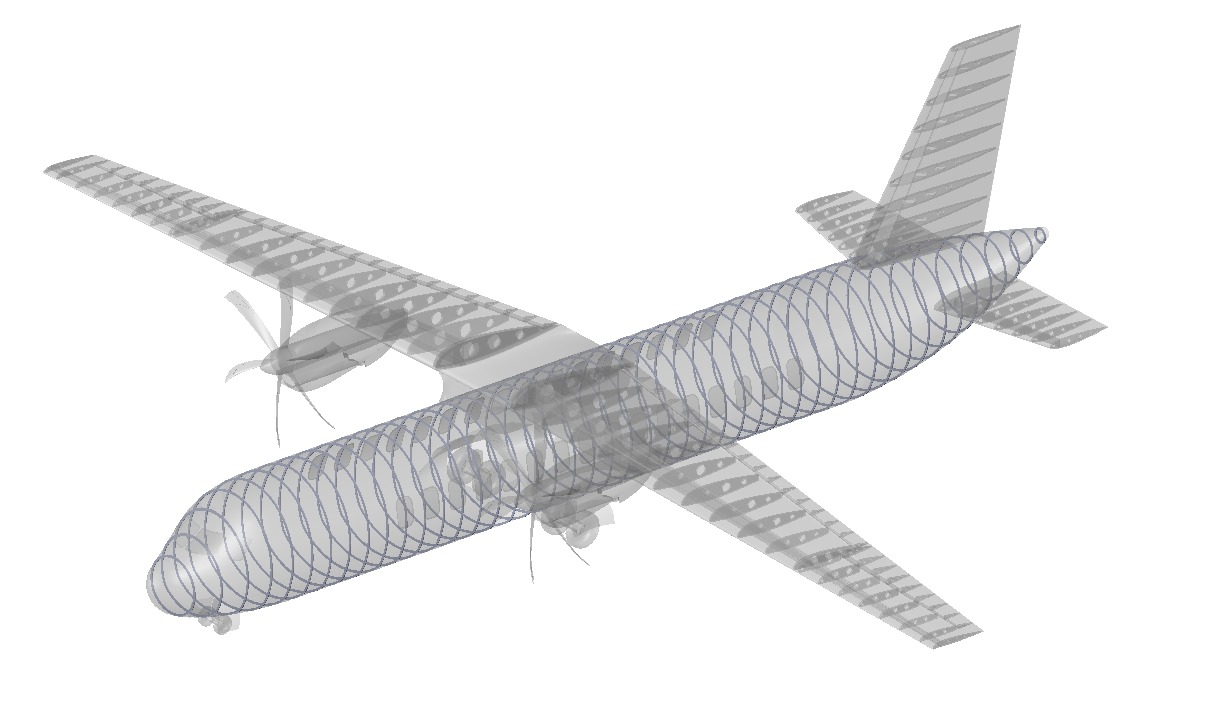
\includegraphics[width=1\textwidth]{Images-3-ProjetoDetalhado/cad-03.jpeg}
    \label{fig:cad_dimensionamento_3}
\end{figure}


\chapter{Configuração Final da Aeronave}
\label{cap:aeronave}

Com base no projeto conceitual e nos dimensionamentos e análises desenvolvidos durante o projeto preliminar, apresenta-se a configuração final proposta para a aeronave. O projeto resultante corresponde a uma aeronave regional turboélice, de asa alta, trem de pouso triciclo retrátil e empenagens convencionais, destinada ao transporte regional de passageiros e à operação adaptável para transporte de cargas.

As vistas apresentadas nas Figuras \ref{vista_lateral_aeronave}, \ref{vista_superior_aeronave} e \ref{vista_frontal_aeronave} sintetizam a configuração externa final da aeronave. Ressalta-se que todas as cotas indicadas nas vistas estão em milímetros.

\begin{figure}[H]
    \centering
    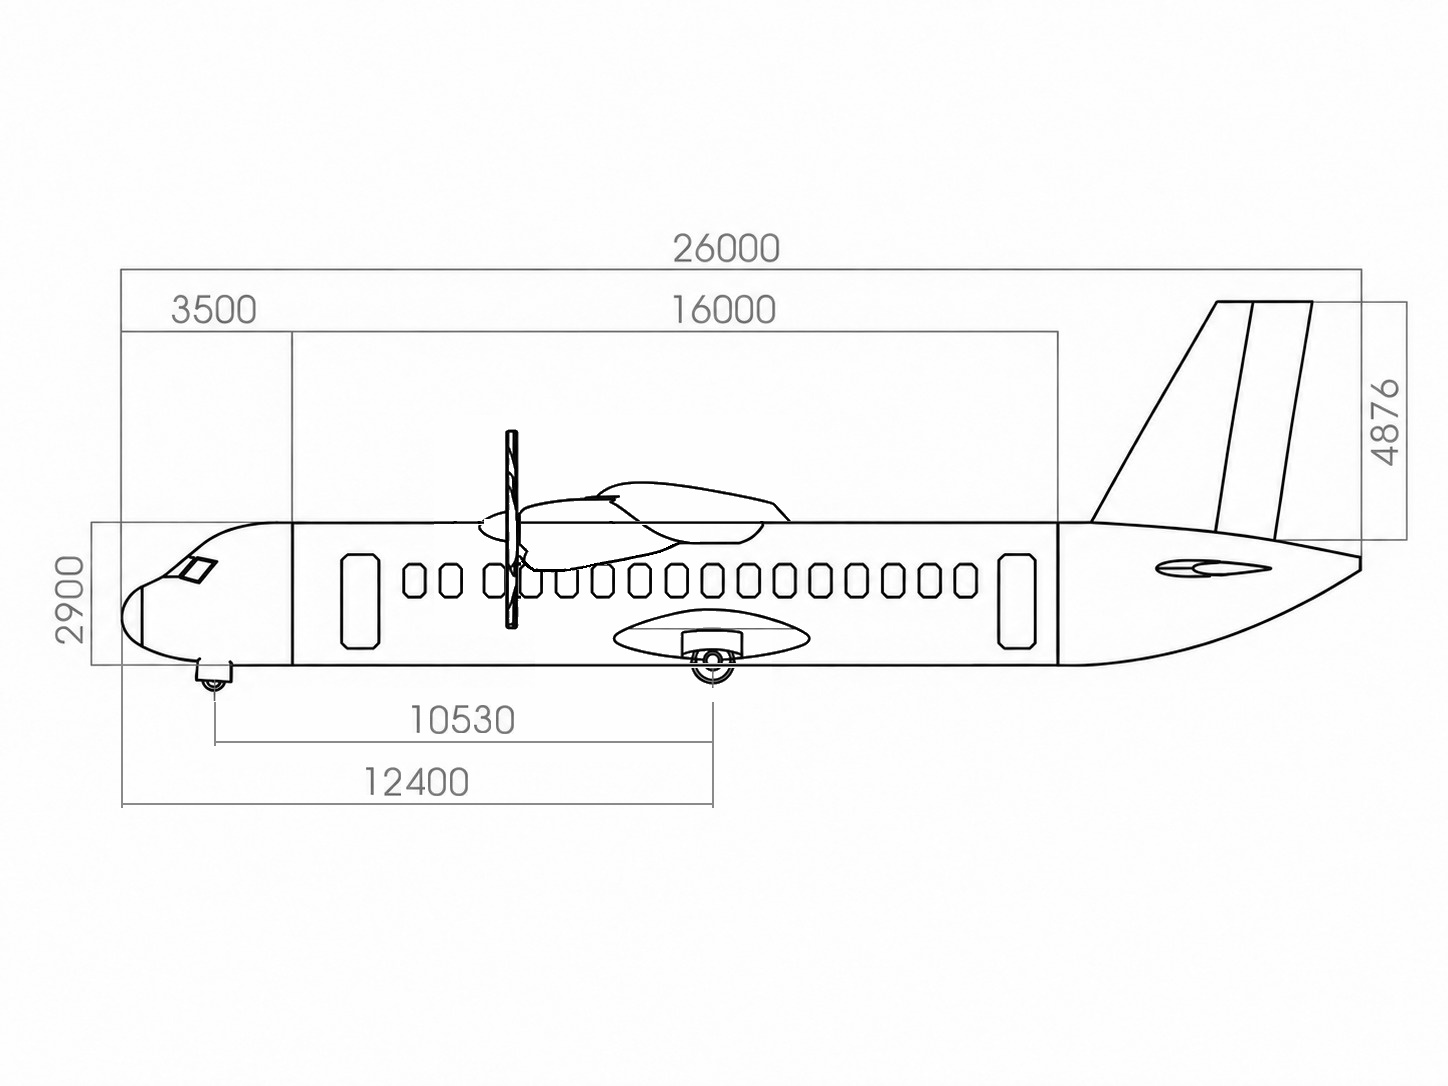
\includegraphics[width=0.92\textwidth]{Images-CG/VistaLateral.jpeg}
    \caption{Vista lateral da configuração final da aeronave.}
    \label{vista_lateral_aeronave}
\end{figure}

\begin{figure}[H]
    \centering
    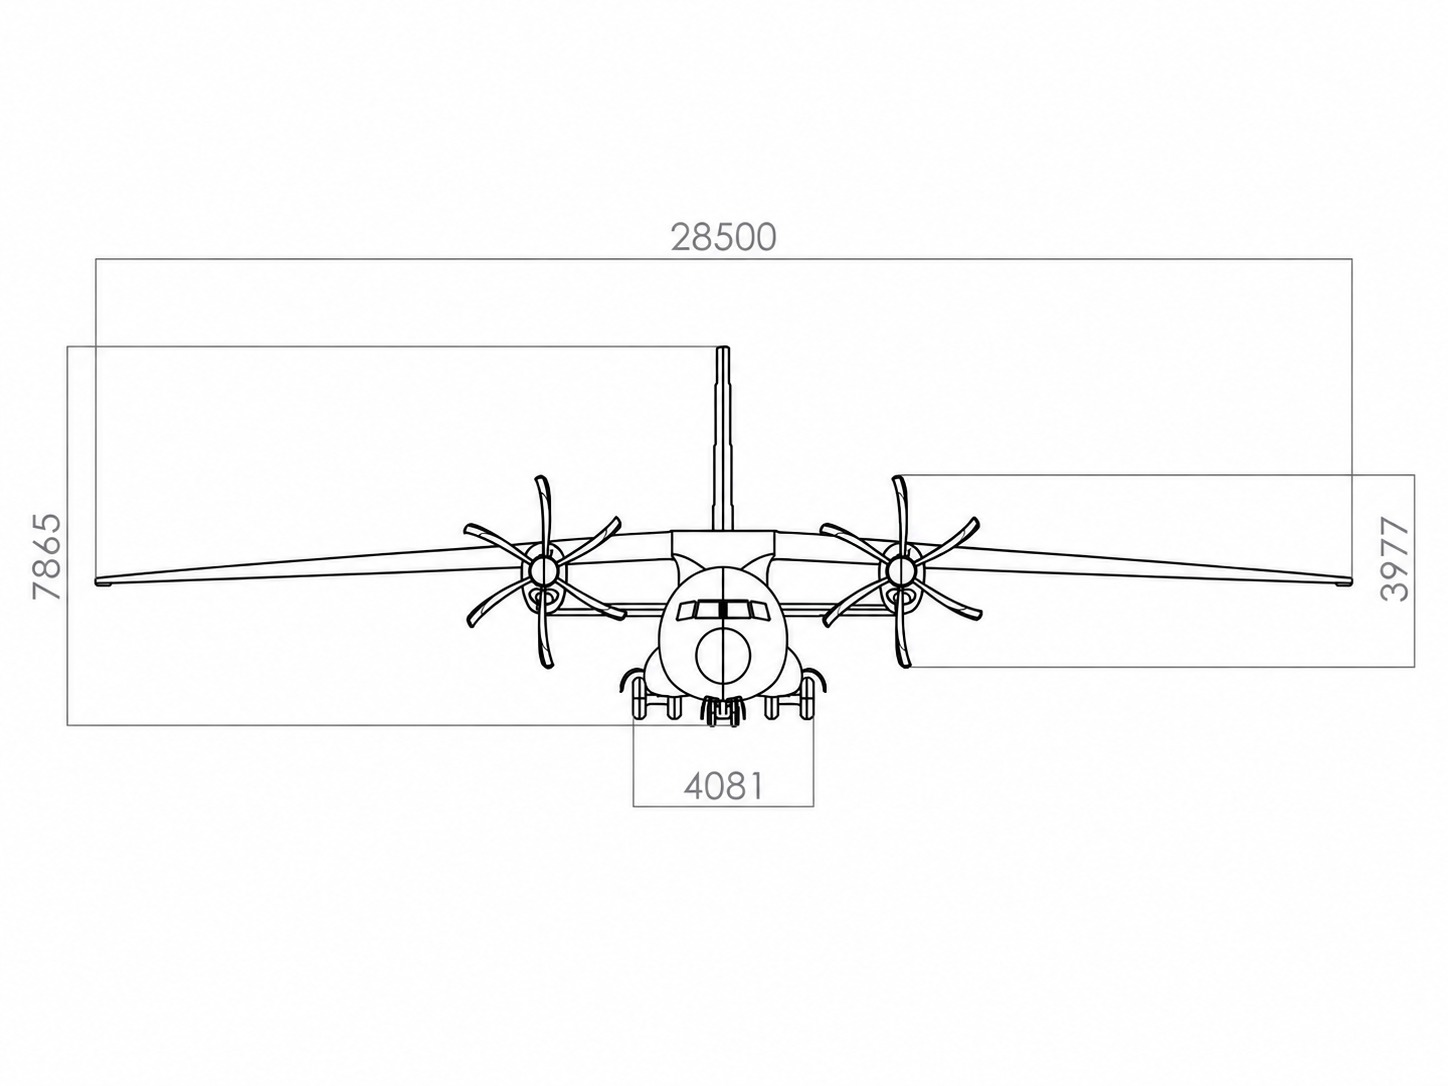
\includegraphics[width=0.92\textwidth]{Images-3-ProjetoDetalhado/VistaFrontal.jpeg}
    \caption{Vista frontal da configuração final da aeronave.}
    \label{vista_frontal_aeronave}
\end{figure}

\begin{figure}[H]
    \centering
    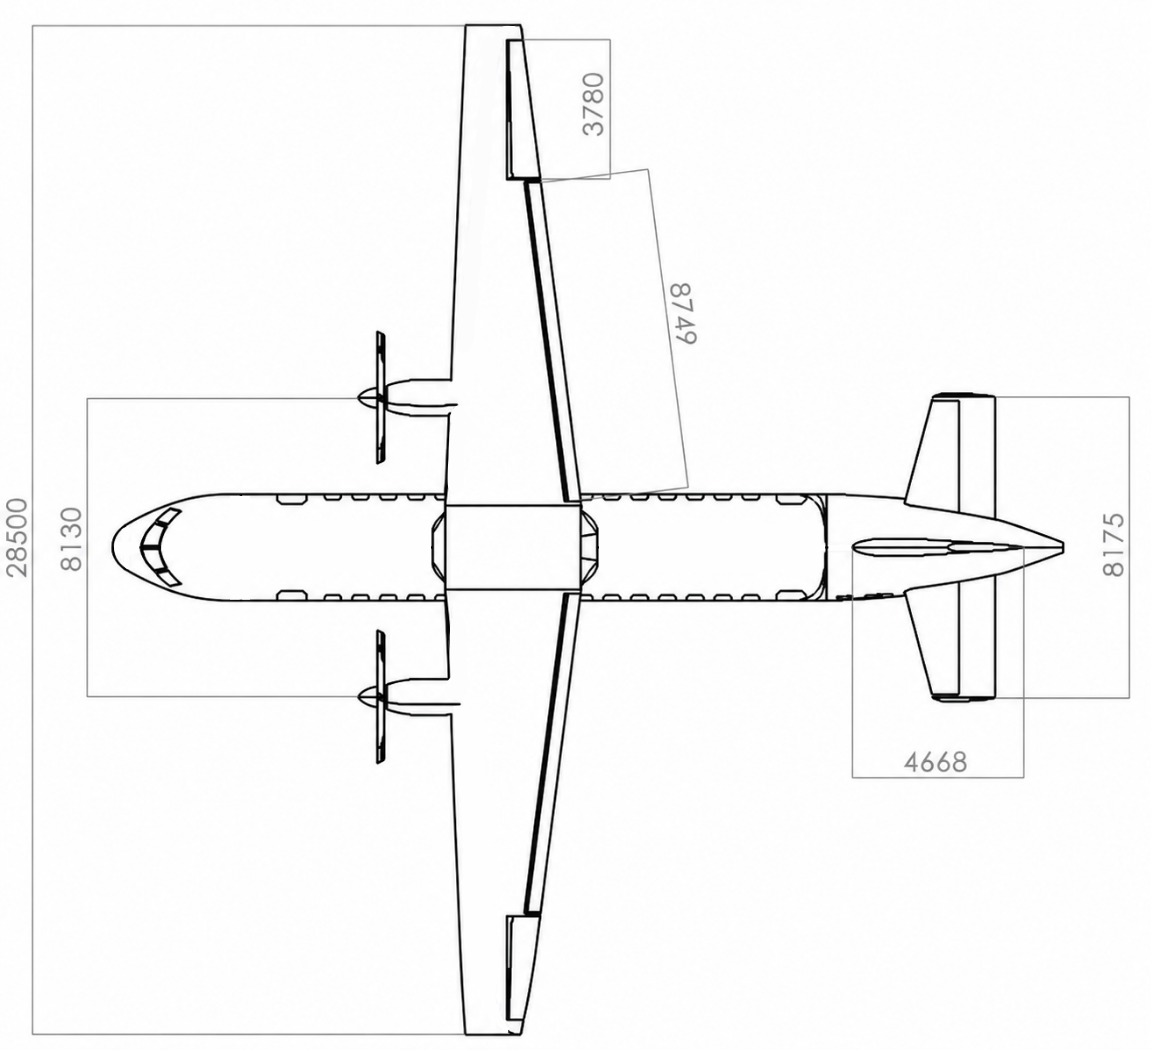
\includegraphics[width=0.8\textwidth]{Images-3-ProjetoDetalhado/VistaSuperior.jpeg}
    \caption{Vista superior da configuração final da aeronave.}
    \label{vista_superior_aeronave}
\end{figure}

Imagens adicionais da aeronave, contemplando outras perspectivas da configuração final, são apresentadas no Anexo.



\clearpage

\section{Resumo Técnico da Aeronave}
\label{sec:resumo_tecnico}

Abaixo são apresentados os principais parâmetros de projeto da aeronave.

% --- TABELA 1: VISÃO GERAL ---
\subsection{Visão Geral e Perfil de Missão}
\begin{table}[htbp]
\centering
\small
\begin{tabularx}{\textwidth}{lX}
\toprule
\textbf{Parâmetro} & \textbf{Especificação} \\
\midrule
Tipo de Aeronave & Transporte Regional (Passageiros e Cargas) \\
Arquitetura & Asa Alta, Empenagem Convencional, Trem de Pouso Triciclo Retrátil \\
Configuração de Passageiros & 64 passageiros (Arranjo 2+2, Pitch de 30 in / 762 mm) \\
Configuração de Cargas & \textit{Quick Change} (Trilhos estruturais, compatível com Paletes IATA PLA) \\
Tripulação de Voo & 2 Pilotos (\textit{Glass Cockpit} com 5 displays LCD) \\
\bottomrule
\end{tabularx}
\caption{Visão geral e perfil de missão da aeronave.}
\label{tab:visao_geral}
\end{table}


% --- TABELA 2: PESOS ---
\subsection{Pesos e Capacidades}
\begin{table}[htbp]
\centering
\small
\begin{tabularx}{\textwidth}{lX}
\toprule
\textbf{Parâmetro} & \textbf{Valor} \\
\midrule
Peso Máximo de Decolagem (MTOW) & 22.680 kgf (50.000 lb) \\
Peso Máximo de Pouso (MLW) & 22.350 kgf (49.273 lb) \\
Peso Máximo Zero Combustível (MZFW) & 19.592 kgf (43.193 lb) \\
Peso Vazio Operacional (OEW) & 13.512 kgf (29.789 lb), com tripulação e \textit{catering} \\
Peso Vazio ($W_E$) & 13.064 kgf (28.801 lb) \\
Carga Paga Máxima & 6.080 kgf (64 passageiros de 84 kg e 11 kg de bagagem cada) \\
Combustível com Carga Paga Máxima & 3.088 kgf (6.808 lb) \\
Capacidade de Combustível & 4.990 kgf (11.000 lb) \\
Envelope de CG & 17,9\% a 45,9\% da CMA (10,79 m a 11,56 m do nariz) \\
\bottomrule
\end{tabularx}
\caption{Pesos limites e capacidades estruturais.}
\label{tab:pesos_capacidades}
\end{table}

% --- TABELA 3: PROPULSÃO ---
\subsection{Grupo Motopropulsor}
\begin{table}[htbp]
\centering
\small
\begin{tabularx}{\textwidth}{lX}
\toprule
\textbf{Parâmetro} & \textbf{Especificação} \\
\midrule
Motores & 2x Pratt \& Whitney PW127M (Turboélice) \\
Potência Máxima (por motor) & 2.475 shp (Total Instalada: 4.950 shp) \\
Hélices & Hamilton Standard 568F (6 pás, passo variável) \\
Carga de Potência ($W/P$) & 4,58 kg/shp \\
\bottomrule
\end{tabularx}
\caption{Especificações do grupo motopropulsor.}
\label{tab:propulsao}
\end{table}

\clearpage

% --- TABELA 4: GEOMETRIA ---
\subsection{Dimensões Principais e Geometria}
\begin{table}[htbp]
\centering
\small
\begin{tabularx}{\textwidth}{llX}
\toprule
\textbf{Componente} & \textbf{Parâmetro} & \textbf{Valor} \\
\midrule
\textbf{Fuselagem} & Comprimento Total & 26,00 m \\
                   & Dimensões Internas da Cabine & 16,00 m (Comp.) $\times$ 2,60 m (Larg.) $\times$ 1,93 m (Alt.) \\
\midrule
\textbf{Asa}       & Envergadura ($b$) / Área ($S$) & 28,50 m / 74,10 m$^2$ \\
                   & Corda Média Aerodinâmica ($\bar{c}$) & 2,75 m \\
                   & Alongamento ($AR$) / Afilamento ($\lambda$) & 10,96 / 0,405 \\
                   & Perfis Aerodinâmicos & NACA 43016 (Raiz) / NACA 43009 (Ponta) \\
\midrule
\textbf{Empenagens} & Empenagem Horizontal & $S = 18,679$ m$^2$ / $b = 8,375$ m / NACA 0012 \\
                   & Empenagem Vertical & $S = 15,359$ m$^2$ / Altura = 4,925 m / NACA 0012 \\
\midrule
\textbf{Trem de Pouso} & Pneus (Principal / Nariz) & H34x10.0R16 (Radial) / 450x190-5 (Diagonal c/ Chine) \\
                       & Freios & Multidisco de Carbono (Cap. Térmica: 8,26 MJ) \\
\bottomrule
\end{tabularx}
\caption{Dimensões principais e características geométricas.}
\label{tab:geometria}
\end{table}

% --- TABELA 5: DESEMPENHO ---
\subsection{Desempenho e Envelope de Voo}
\begin{table}[htbp]
\centering
\small
\begin{tabularx}{\textwidth}{lX}
\toprule
\textbf{Parâmetro} & \textbf{Valor de Projeto} \\
\midrule
Velocidade de Cruzeiro de Projeto ($V_C$) & 230 kt EAS (\S 25.335) \\
Velocidade de Cruzeiro de Máximo Alcance & 193 kt TAS (357 km/h) a 20.000 ft \\
Velocidade Máxima em Cruzeiro & 247,1 kt (457,6 km/h) \\
Velocidade Máxima de Decolagem & 209,0 kt (387,0 km/h) \\
Velocidade de Estol ($V_S$) & 107,9 kt (Config. Pouso) / 125,8 kt (Config. Decolagem) \\
Distância Total de Decolagem & 1.102 m (3.614 ft) --- Ao nível do mar, ISA, MTOW \\
Distância Física de Pouso & 797 m (2.616 ft) --- Ao nível do mar, ISA, MLW \\
Teto de Serviço / Teto Absoluto & 24.438 ft (7.449 m) / 26.115 ft (7.960 m) \\
Alcance com Cabine Cheia e Reservas IFR & 925 NM (1.713 km); requisito: 800 NM \\
Autonomia do Trecho de Cruzeiro (cabine cheia) & 4,7 horas \\
Razão de Subida Máx. (Cruzeiro) & 1,23 m/s (aprox. 242 ft/min) \\
\bottomrule
\end{tabularx}
\caption{Parâmetros estimados de desempenho e operação.}
\label{tab:desempenho}
\end{table}


% ==========================================
% SEÇÃO DE ANEXOS A SER INCLUÍDA NO FINAL
% ==========================================

\chapter{Anexos}

\begin{figure}[H]
    \centering
    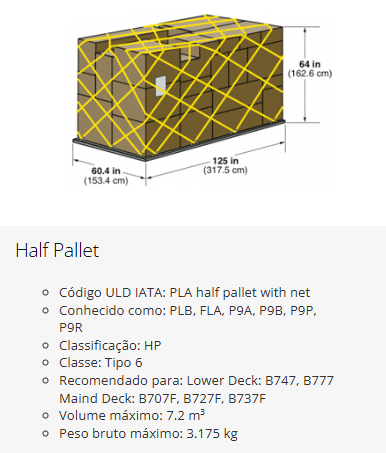
\includegraphics[width=0.5\linewidth]{images/half pallet.png}
    \caption{Palete Padrão\cite{sideral_comex_containers}}
    \label{fig:palete}
\end{figure}

\section{Integrantes do Projeto}

Abaixo segue a lista dos integrantes do projeto e suas respectivas matrículas:

\vspace{0.5cm}

\begin{table}[H]
\centering
\begin{tabular}{ll}
\hline
\textbf{Nome} & \textbf{Matrícula} \\ \hline
Caio Fernandes Rickli Costa & 2020022308 \\
Carolina Chaves Ferrari de Lima & 2021015666 \\
Filipe Gomes Ferreira e Silva & 2022060355 \\
Flaubert Silva Ferreira & -- \\
Gabriel Fernando Duarte Marques & 2022060134 \\
Gabriel Henrique Ferreira Soares & 2019070418 \\
Gabriela Araujo Machado & 2019022367 \\
Luísa Vilela Gonçalves & 2020069380 \\
Pedro Henrique Oliveira Roquette & 2022060410 \\
Pedro Palma Maia Ornelas & 2022095612 \\
Rodrigo Pena Teobaldo & 2022060312 \\
Saulo de Lacerda Pires & 2020022685 \\
Vicente Fernandes de Queiroz Neto & 2022060142 \\
Victor Gomes Teixeira & -- \\
Vitor da Silva Gonçalves & 2022045291 \\
Vitor de Jesus Mendes & 2022421170 \\ \hline
\end{tabular}
\end{table}



\section{Informações adicionais da dinâmica longitudinal}

\subsection{Gráficos CG traseiro}

\begin{figure}[H]
    \centering
    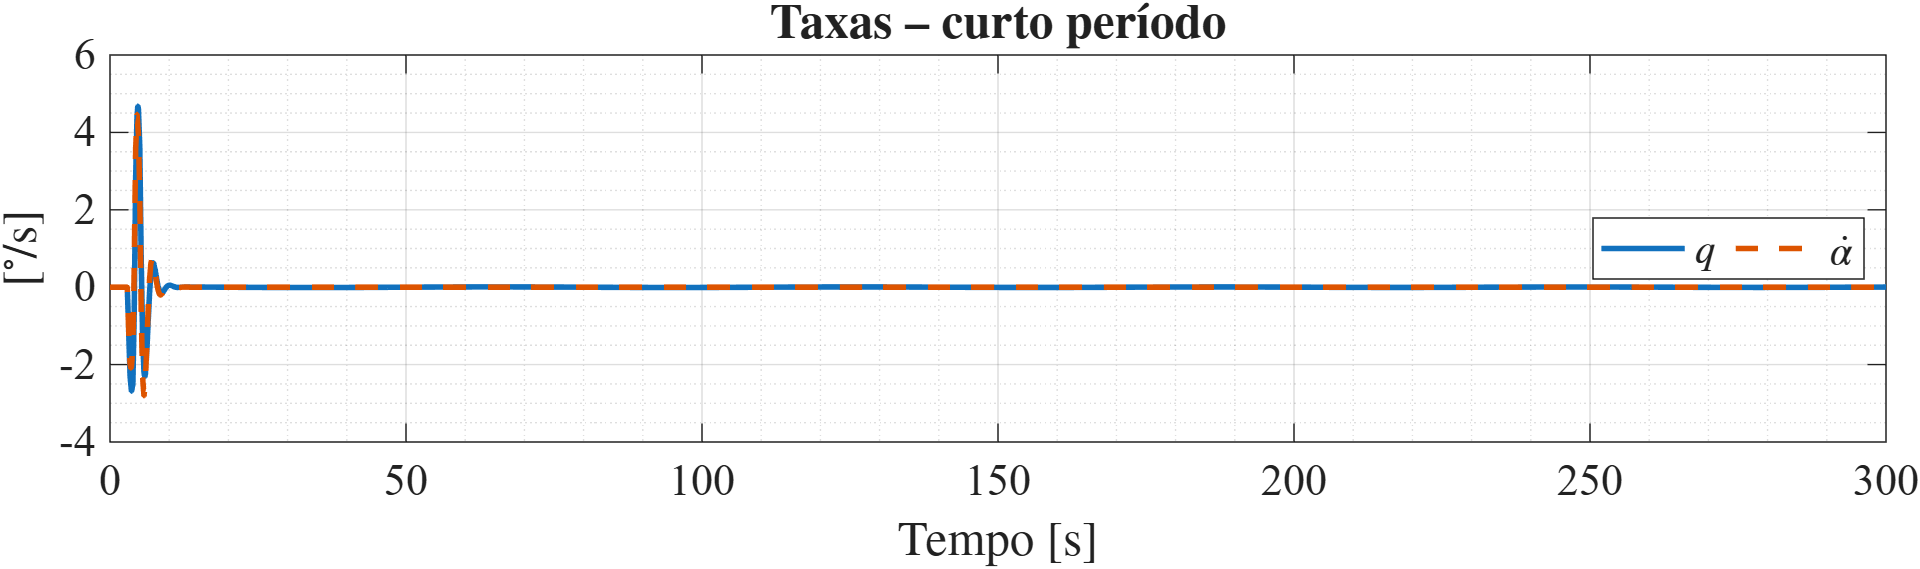
\includegraphics[width=0.9\linewidth]{images/estabilidade/Taxas_CG_traseiro.png}
    \caption{Evolução de q e $\dot{\alpha}$ para CG traseiro}
    \label{fig:placeholder}
\end{figure}

\begin{figure}[H]
    \centering
    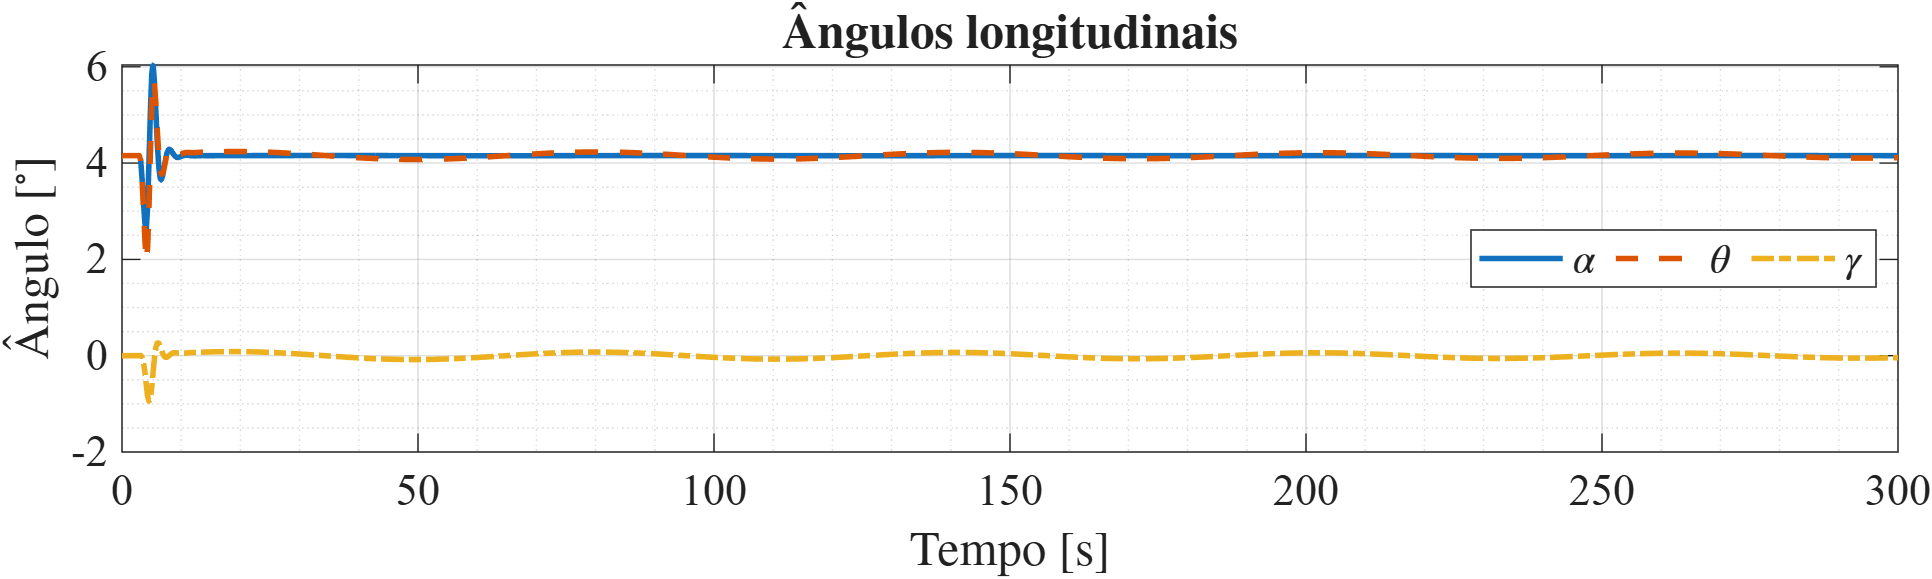
\includegraphics[width=0.9\linewidth]{images/estabilidade/angulos_300s_CG_traseiro.png}
    \caption{Evolução de $\alpha$, $\theta$ e $\gamma$ para CG traseiro}
    \label{fig:placeholder}
\end{figure}

\subsection{Gráficos CG dianteiro}


\begin{figure}[H]
    \centering
    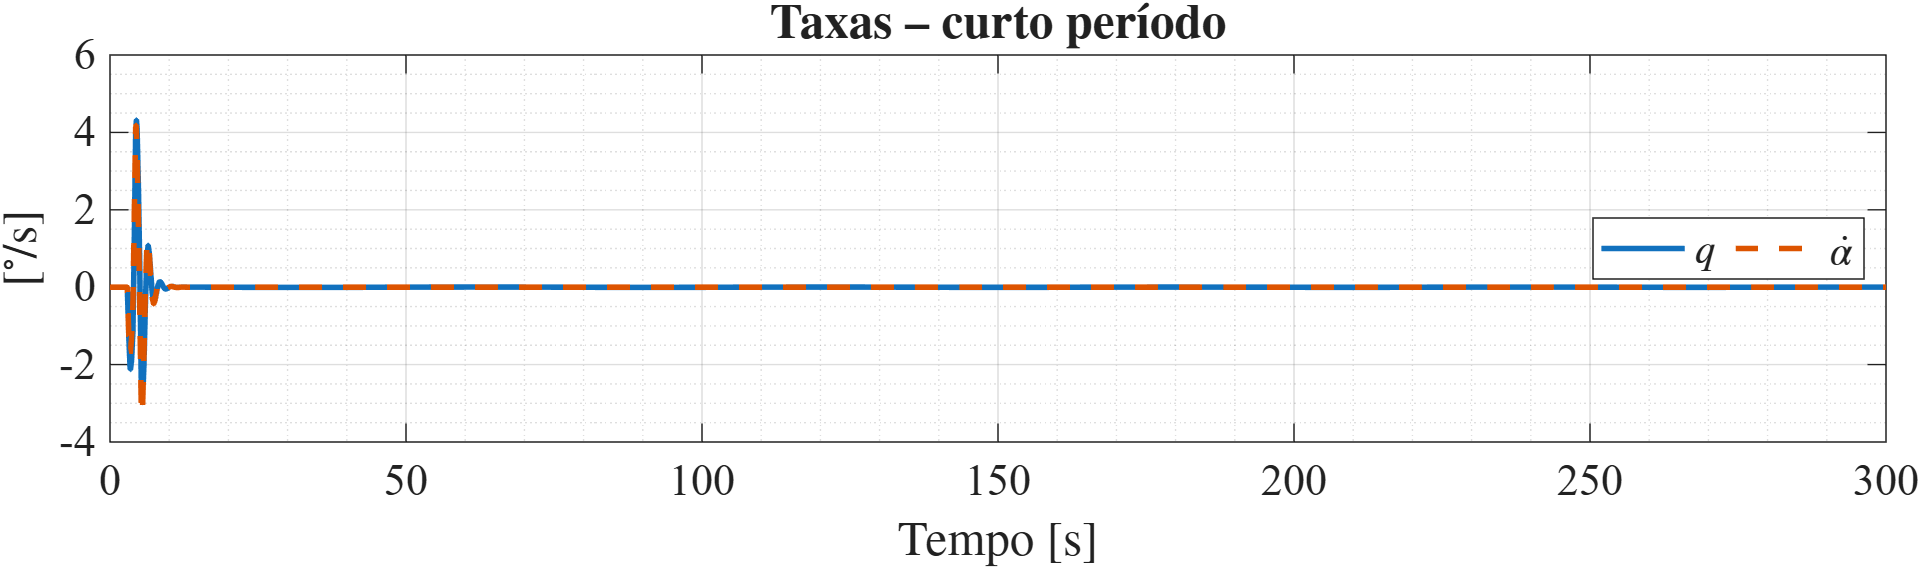
\includegraphics[width=0.9\linewidth]{images/estabilidade/Taxas_CG_dianteiro.png}
    \caption{Evolução de q e $\dot{\alpha}$ para CG dianteiro}
    \label{fig:placeholder}
\end{figure}

\begin{figure}[H]
    \centering
    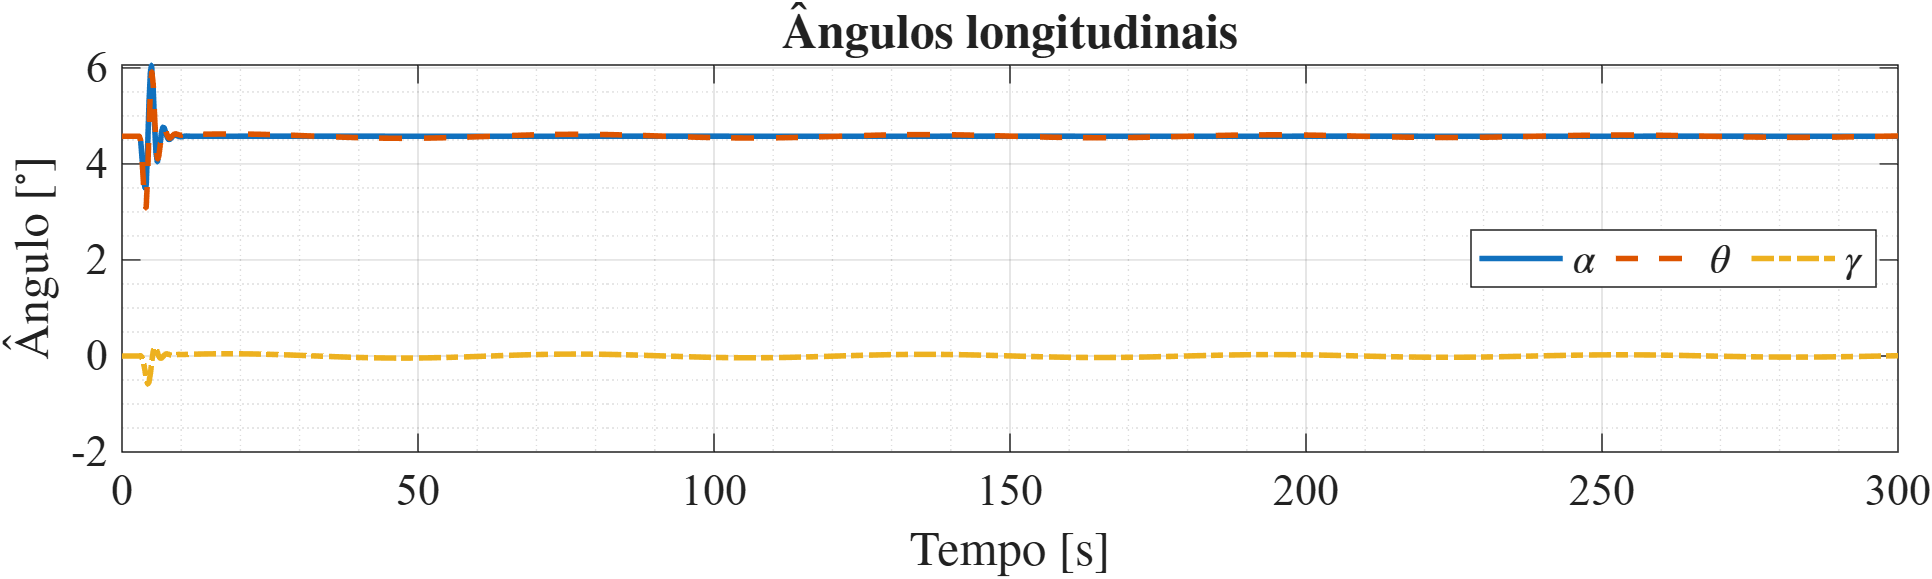
\includegraphics[width=0.9\linewidth]{images/estabilidade/angulos_300s_CG_dianteiro.png}
    \caption{Evolução de $\alpha$, $\theta$ e $\gamma$ para CG dianteiro}
    \label{fig:placeholder}
\end{figure}


\subsection{Derivadas de estabilidade}

\begin{table}[H]
    \centering
    \caption{Derivadas de estabilidade longitudinal e parâmetros associados para as condições extremas de CG, obtidas no AVL a 20000 ft de altitude.}
    \begin{tabular}{|l|c|c|}
       \hline
       \textbf{Parâmetro} & \textbf{CG dianteiro} & \textbf{CG traseiro} \\
       \hline
       $h_{CG}$ (\%  $\bar{c}$)        & $0{,}179$   & $0{,}459$  \\
       \hline
       Margem estática (SM)              & $0{,}561$   & $0{,}281$  \\
       \hline
       $C_{L_0}$                         & $0{,}1916$  & $0{,}1916$ \\
       \hline
       $C_{L_\alpha}$ [rad$^{-1}$]       & $5{,}816$   & $5{,}816$  \\
       \hline
       $C_{L_q}$ [rad$^{-1}$]            & $14{,}532$  & $11{,}274$ \\
       \hline
       $C_{L_\eta}$ [rad$^{-1}$]         & $0{,}636$   & $0{,}636$  \\
       \hline
       $C_{D_0}$                         & $0{,}00227$ & $0{,}00227$\\
       \hline
       $C_{m_0}$                         & $0{,}0150$  & $0{,}0687$ \\
       \hline
       $C_{m_\alpha}$ [rad$^{-1}$]       & $-3{,}265$  & $-1{,}636$ \\
       \hline
       $C_{m_q}$ [rad$^{-1}$]            & $-39{,}323$ & $-34{,}338$\\
       \hline
       $C_{m_\eta}$ [rad$^{-1}$]         & $-2{,}827$  & $-2{,}649$ \\
       \hline
    \end{tabular}
    \label{tab:derivadas_long_anexo}
\end{table}


\section{Dimensões Antropométricas de Pilotos}
\begin{table}[H]
    \centering
    \caption{Dimensões anatômicas estáticas detalhadas para ergonomia da cabine [cm].}
    \label{tab:dimensoes_anatomicas_cabine}
    \resizebox{\textwidth}{!}{%
    \begin{tabular}{lcccccc}
    \hline
        \textbf{Dimensão} &
        \multicolumn{3}{c}{\textbf{Masculino (M)}} &
        \multicolumn{3}{c}{\textbf{Feminino (F)}} \\
        \cline{2-7}
        & \textbf{5º} & \textbf{50º} & \textbf{95º}
        & \textbf{5º} & \textbf{50º} & \textbf{95º} \\
    \hline
        1 - Altura em posição sentada &
        85,8 & 91,4 & 97,2 & 79,5 & 85,1 & 91,0 \\

        2 - Altura dos olhos, sentado &
        73,5 & 79,2 & 84,8 & 68,5 & 73,8 & 79,4 \\

        3 - Altura do ombro, sentado &
        54,9 & 59,8 & 64,6 & 50,9 & 55,5 & 60,4 \\

        4 - Altura do cotovelo, sentado &
        18,4 & 23,2 & 27,4 & 17,6 & 22,1 & 26,4 \\

        5 - Espessura da coxa &
        14,9 & 16,8 & 19,0 & 14,0 & 15,8 & 18,0 \\

        6 - Altura do joelho, sentado &
        51,4 & 55,8 & 60,6 & 47,4 & 49,8 & 56,0 \\

        7 - Altura poplítea, sentado &
        39,5 & 43,3 & 47,6 & 35,1 & 38,9 & 42,9 \\

        8 - Comprimento antebraço-ponta do dedo &
        44,8 & 48,3 & 52,4 & 40,6 & 44,2 & 48,3 \\

        Alcance funcional do braço &
        73,9 & 80,0 & 86,7 & 67,7 & 73,4 & 79,7 \\

        9 - Largura dos ombros (bideltoide) &
        45,0 & 49,1 & 53,5 & 39,7 & 43,1 & 47,2 \\

        10 - Largura entre cotovelos &
        47,8 & 54,5 & 62,1 & 41,5 & 46,7 & 52,8 \\
    \hline
\end{tabular}%
}

\vspace{0.2cm}
\small Fonte: Adaptado de FAA HFDS \cite{FAA_HFDS}, Seção 5.12.3.2.
\end{table}

\section{Comparação entre Tecnologias de Freios}
\begin{table}[H]
    \centering
    \caption{Comparação entre tecnologias de freios aeronáuticos.}
    \vspace{0.2cm}

    \renewcommand{\arraystretch}{1.6}
    \setlength{\tabcolsep}{6pt}

    \begin{tabular}{|p{3.5cm}|p{3.2cm}|p{3.5cm}|p{5.2cm}|}
        \hline
        \textbf{Propriedade / Característica} &
        \textbf{Freios de Aço} &
        \textbf{Freios de Carbono} &
        \textbf{Impacto Técnico no Projeto} \\
        \hline

        Peso do Conjunto de Freios
        & Elevado (referência)
        & Redução de 35\% a 42\% em massa
        & Redução do OEW e aumento da capacidade de carga paga ou combustível \\
        \hline

        Condutividade Térmica
        & Moderada
        & Elevada
        & Dissipação térmica mais eficiente e menor risco de superaquecimento \\
        \hline

        Resistência Térmica e Vida Útil
        & Perda de eficiência acima de $500^\circ$C; vida útil entre 800 e 1200 ciclos
        & Operação estável até $1200^\circ$C; vida útil entre 1500 e 3000 ciclos
        & Maior confiabilidade operacional e redução de manutenção \\
        \hline

        Custo de Aquisição Inicial
        & Baixo
        & Elevado
        & Maior custo inicial compensado pela durabilidade e menor custo operacional \\
        \hline
    \end{tabular}

    \label{tab:comparacao_freios}
\end{table}

\section{Imagens Adicionais da Aeronave}
\begin{figure}[H] 
    \centering 
    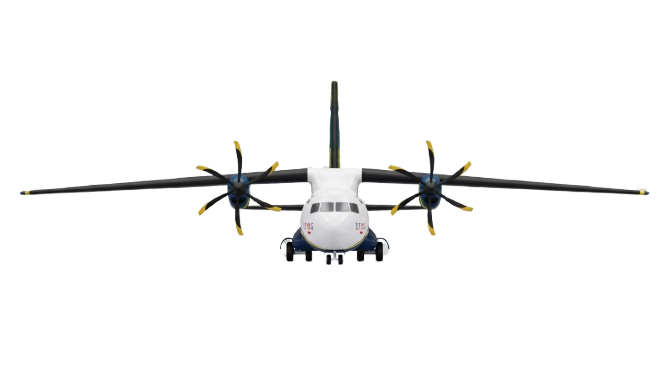
\includegraphics[width=1.00\textwidth]{Images-3-ProjetoDetalhado/Render_Frontal_v2.png} \caption{Vista frontal da configuração final da aeronave.} 
    \label{render_frontal} 
\end{figure}

% \begin{figure}[H] 
%     \centering 
%     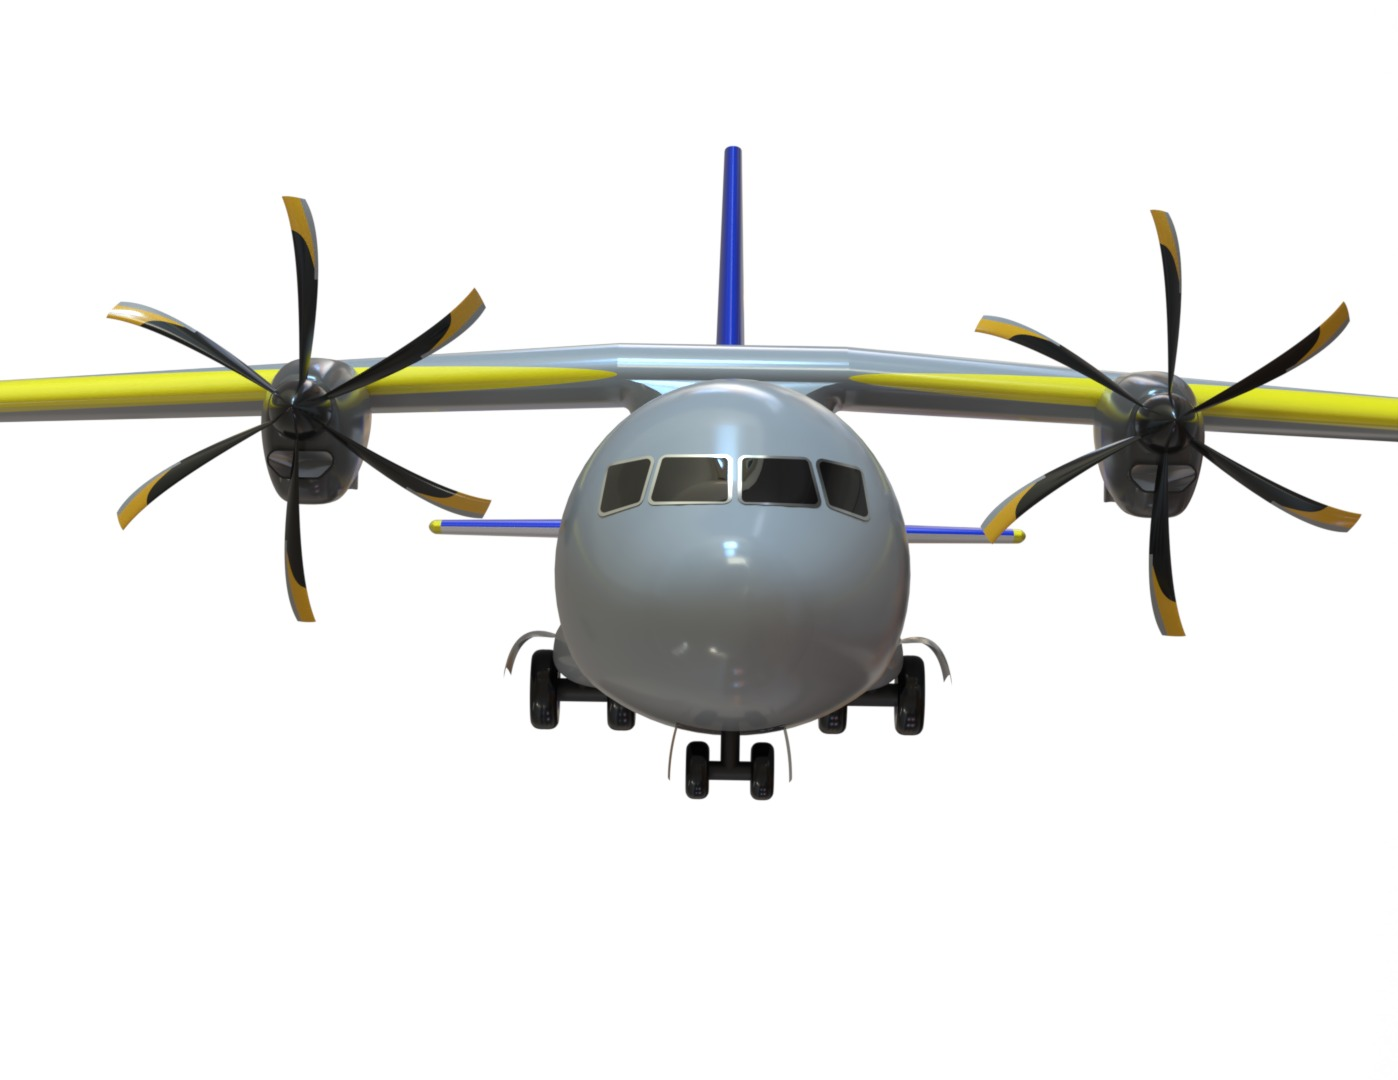
\includegraphics[width=0.85\textwidth]{Images-3-ProjetoDetalhado/render_frontal.jpeg} \caption{Renderização frontal da configuração final da aeronave.} 
%     \label{render_frontal} 
% \end{figure}

\begin{figure}[H] 
    \centering 
    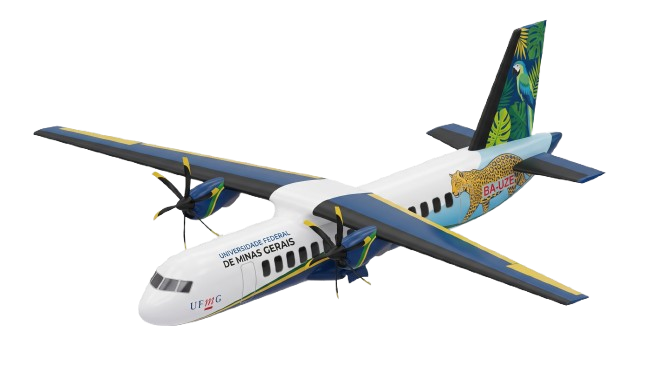
\includegraphics[width=1.0\textwidth]{Images-3-ProjetoDetalhado/render_isometrico.png} \caption{Vista em perspectiva da configuração final da aeronave.} 
    \label{render_frontal} 
\end{figure}

% \begin{figure}[H] 
%     \centering 
%     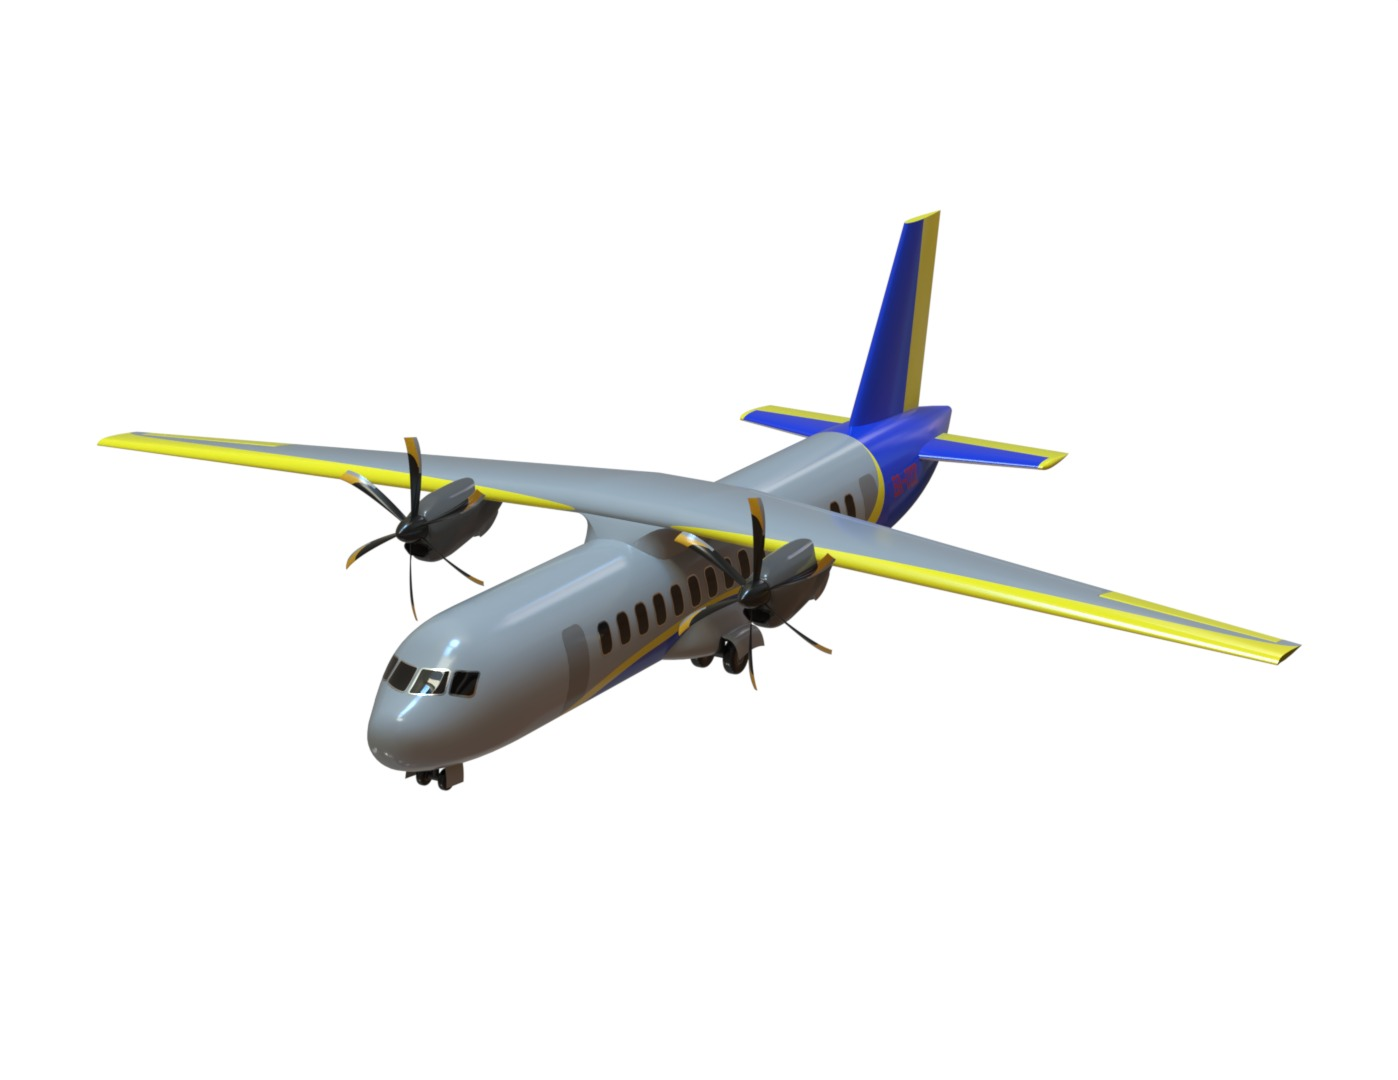
\includegraphics[width=1.0\textwidth]{Images-3-ProjetoDetalhado/render_perspectiva.jpeg} \caption{Renderização em perspectiva da configuração final da aeronave.} 
%     \label{render_frontal} 
% \end{figure}



\begin{figure}[H] 
    \centering 
    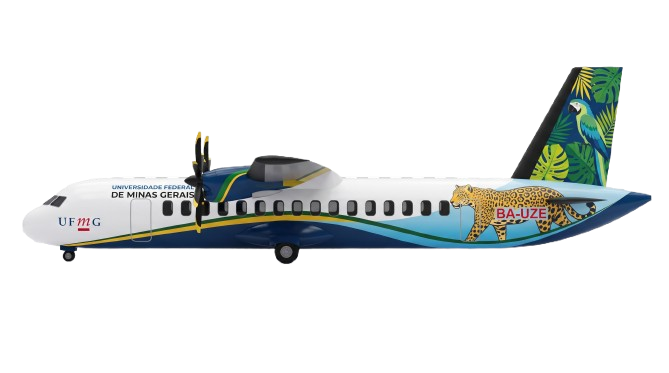
\includegraphics[width=1.0\textwidth]{Images-3-ProjetoDetalhado/render_lateral.jpeg} \caption{Vista Lateral da Aeronave} \label{render_lateral_dianteira} 
\end{figure}


% \begin{figure}[H] 
%     \centering 
%     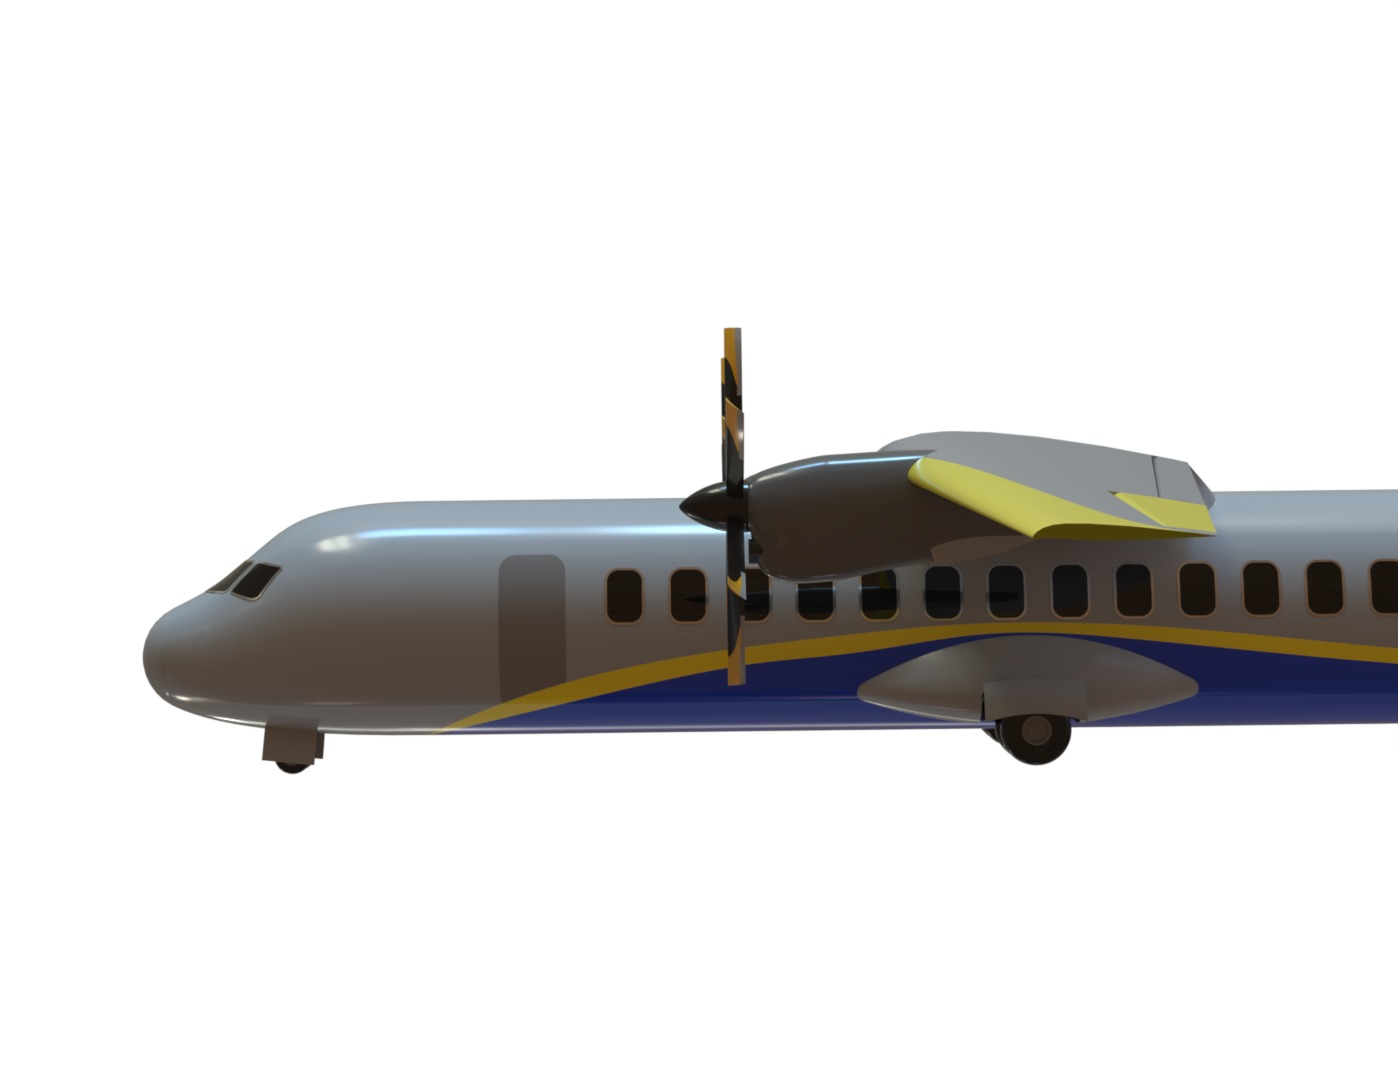
\includegraphics[width=0.68\textwidth]{Images-3-ProjetoDetalhado/render_lateral_dianteira.jpeg} \caption{Detalhe lateral dianteiro da aeronave, evidenciando a fuselagem, a nacele, o trem de pouso e a asa.} \label{render_lateral_dianteira} 
% \end{figure}

% \begin{figure}[H] 
%     \centering 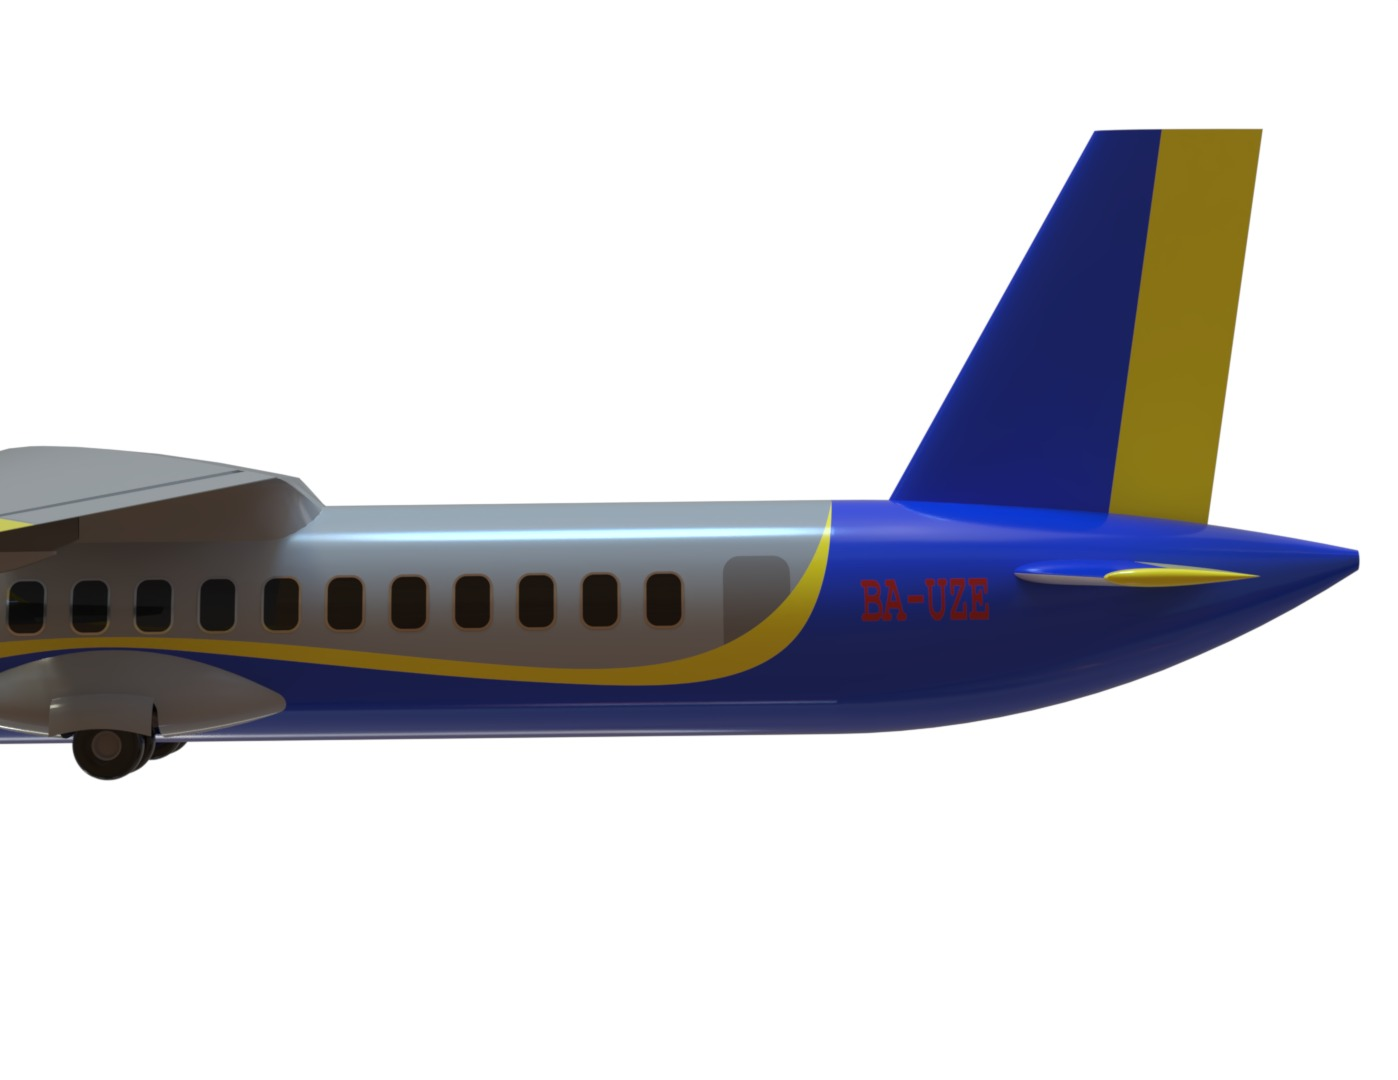
\includegraphics[width=0.68\textwidth]{Images-3-ProjetoDetalhado/render_traseira.jpeg} \caption{Detalhe da região traseira da aeronave, evidenciando as empenagens e o cone de cauda.} 
%     \label{render_traseira} 
% \end{figure} 


\subsection*{Projetos 1}

\begin{xltabular}{\textwidth}{|X|X|X|}
\caption{Distribuição de Responsabilidades por Seção -- Projetos 1} \label{tab:responsabilidades} \\

\hline
\textbf{Tópico} & \textbf{Execução} & \textbf{Revisão} \\
\hline
\endfirsthead % CORREÇÃO: Comando sem chavetas

\multicolumn{3}{c}{{\tablename\ \thetable{} -- Continuação da página anterior}} \\
\hline
\textbf{Tópico} & \textbf{Execução} & \textbf{Revisão} \\
\hline
\endhead % CORREÇÃO: Comando sem chavetas

\hline
\multicolumn{3}{r}{{Continua na próxima página...}} \\
\endfoot % CORREÇÃO: Comando sem chavetas

\hline
\endlastfoot % CORREÇÃO: Comando sem chavetas

% --- CONTEÚDO DA TABELA ---
Análise de mercado & Pedro Ornelas e Gabriel Soares & Carolina, Gabriela Machado, Gabriel Marques, Pedro Roquette, Rodrigo Vicente e Saulo Lacerda \\ \hline

Estudo Comparativo & Carolina, Gabriela Machado, Gabriel Marques, Pedro Roquette, Rodrigo e Vicente & Pedro Ornelas, Gabriel Soares e Saulo Lacerda \\
\hline

\multicolumn{3}{|c|}{\textbf{Projeto Conceitual}} \\
\hline

Geometria Interna & Carolina e Pedro Roquette & Gabriel Marques e Rodrigo \\ \hline

Geometria da Asa & Gabriela Machado & Gabriel Marques e Rodrigo \\ \hline

Geometria das Empenagens & Pedro Ornelas e Vicente & Gabriela Machado e Saulo Lacerda \\ \hline

Escolha de Propulsão & Gabriel Soares & Pedro Roquette\\ \hline

Estudo e Definição de Número de Pás de Hélice & Victor Teixeira & \\ \hline

Estimativa de pesos & Gabriel Soares & Gabriela Machado \\ \hline

Estimativa do CG & Carolina & Pedro Roquette \\ \hline

Esboços Iniciais & Gabriel Marques e Rodrigo & \\
\hline

\multicolumn{3}{|c|}{\textbf{Projeto Preliminar}} \\
\hline

Definição do Perfil da Asa & Rodrigo & Pedro Ornelas \\ \hline

Dimensionamento dos Flaps & Rodrigo & Pedro Ornelas \\ \hline

Geometria das Empenagens e Superfícies de Controle & Pedro Ornelas e Vicente & \\ \hline

Geometria Interna & Carolina e Saulo Lacerda & \\ \hline

Dimensionamento de Pneus e Freios & Gabriel Soares, Gabriela Machado e Filipe Gomes & \\ \hline

Aprofundamento do Estudo do CG & Carolina & Pedro Ornelas \\
\hline

\multicolumn{3}{|c|}{\textbf{Aerodinâmica e Desempenho}} \\
\hline

Cálculo estimado da Polar de Arrasto & Gabriel Marques e Vicente & \\ \hline

Cálculo das Potências & & Pedro Ornelas e Gabriel Marques \\ \hline

Velocidades máximas e mínimas & & Pedro Ornelas e Gabriel Marques \\ \hline

Distâncias de Decolagem e Pouso & Pedro Roquette & \\ \hline

Voo em curva & Pedro Roquette & Pedro Ornelas \\ \hline

Autonomia e Alcance & Pedro Roquette & Carolina \\ \hline

Envelope de Voo & Vicente & \\ \hline

Desempenho de Subida & Vicente & \\ \hline

Diagrama de Missão & & Carolina \\ \hline

Resumo dos Cálculos de Desempenho & Pedro Roquette & \\
\hline

Estabilidade longitudinal preliminar & Pedro Ornelas, Vicente & \\ \hline

\end{xltabular}

\subsection*{Projetos 2}

\begin{xltabular}{\textwidth}{|X|X|}
\caption{Distribuição de Responsabilidades por Seção -- Projetos 2}
\label{tab:responsabilidades_p2} \\

\hline
\textbf{Tópico} & \textbf{Execução} \\
\hline
\endfirsthead

\multicolumn{2}{c}{{\tablename\ \thetable{} -- Continuação da página anterior}} \\
\hline
\textbf{Tópico} & \textbf{Execução} \\
\hline
\endhead

\hline
\multicolumn{2}{r}{{Continua na próxima página...}} \\
\endfoot

\hline
\endlastfoot

% --- CONTEÚDO DA TABELA ---

Requisitos e Referências
& Luísa Vilela \\
\hline

Definição do Material
& Gabriel Soares \\
\hline

Revisão de Aerodinâmica
& Vitor Gonçalves e Pedro Roquette \\
\hline

Revisão de Desempenho
& Vitor Gonçalves, Pedro Roquette e Gabriel Marques\\
\hline

Revisão de Estabilidade e Controle
& Vicente Neto e Vitor Mendes \\
\hline

Revisão de Trem de Pouso e Sistemas
& Pedro Ornelas e Filipe Gomes \\
\hline

Ergonomia da Cabine
& Saulo Lacerda \\
\hline

Alterações na Geometria Externa
& Gabriela Machado e Caio Rickli \\
\hline

Cálculos de Peso e CG & Carolina Ferrari \\
\hline

Desenho da longarina, nervuras e vista em corte da fuselagem
& Gabriel Marques, Rodrigo Pena, Flaubert Ferreira, Victor Teixeira e Gabriel Soares \\
\hline

Cargas na Asa e Empenagens
& Vitor Gonçalves \\
\hline

Dimensionamento Estrutural
& Flaubert Ferreira \\
\hline

Dimensionamento do Revestimento
& Vitor Mendes \\
\hline

Materiais da Construção 
& Gabriel Soares e Saulo Lacerda \\
\hline

Dimensionamento do Berço do Motor 
& Gabriel Soares e Saulo Lacerda \\
\hline

\end{xltabular}

\includepdf[pages=-, angle=90]{detalhamento.pdf}

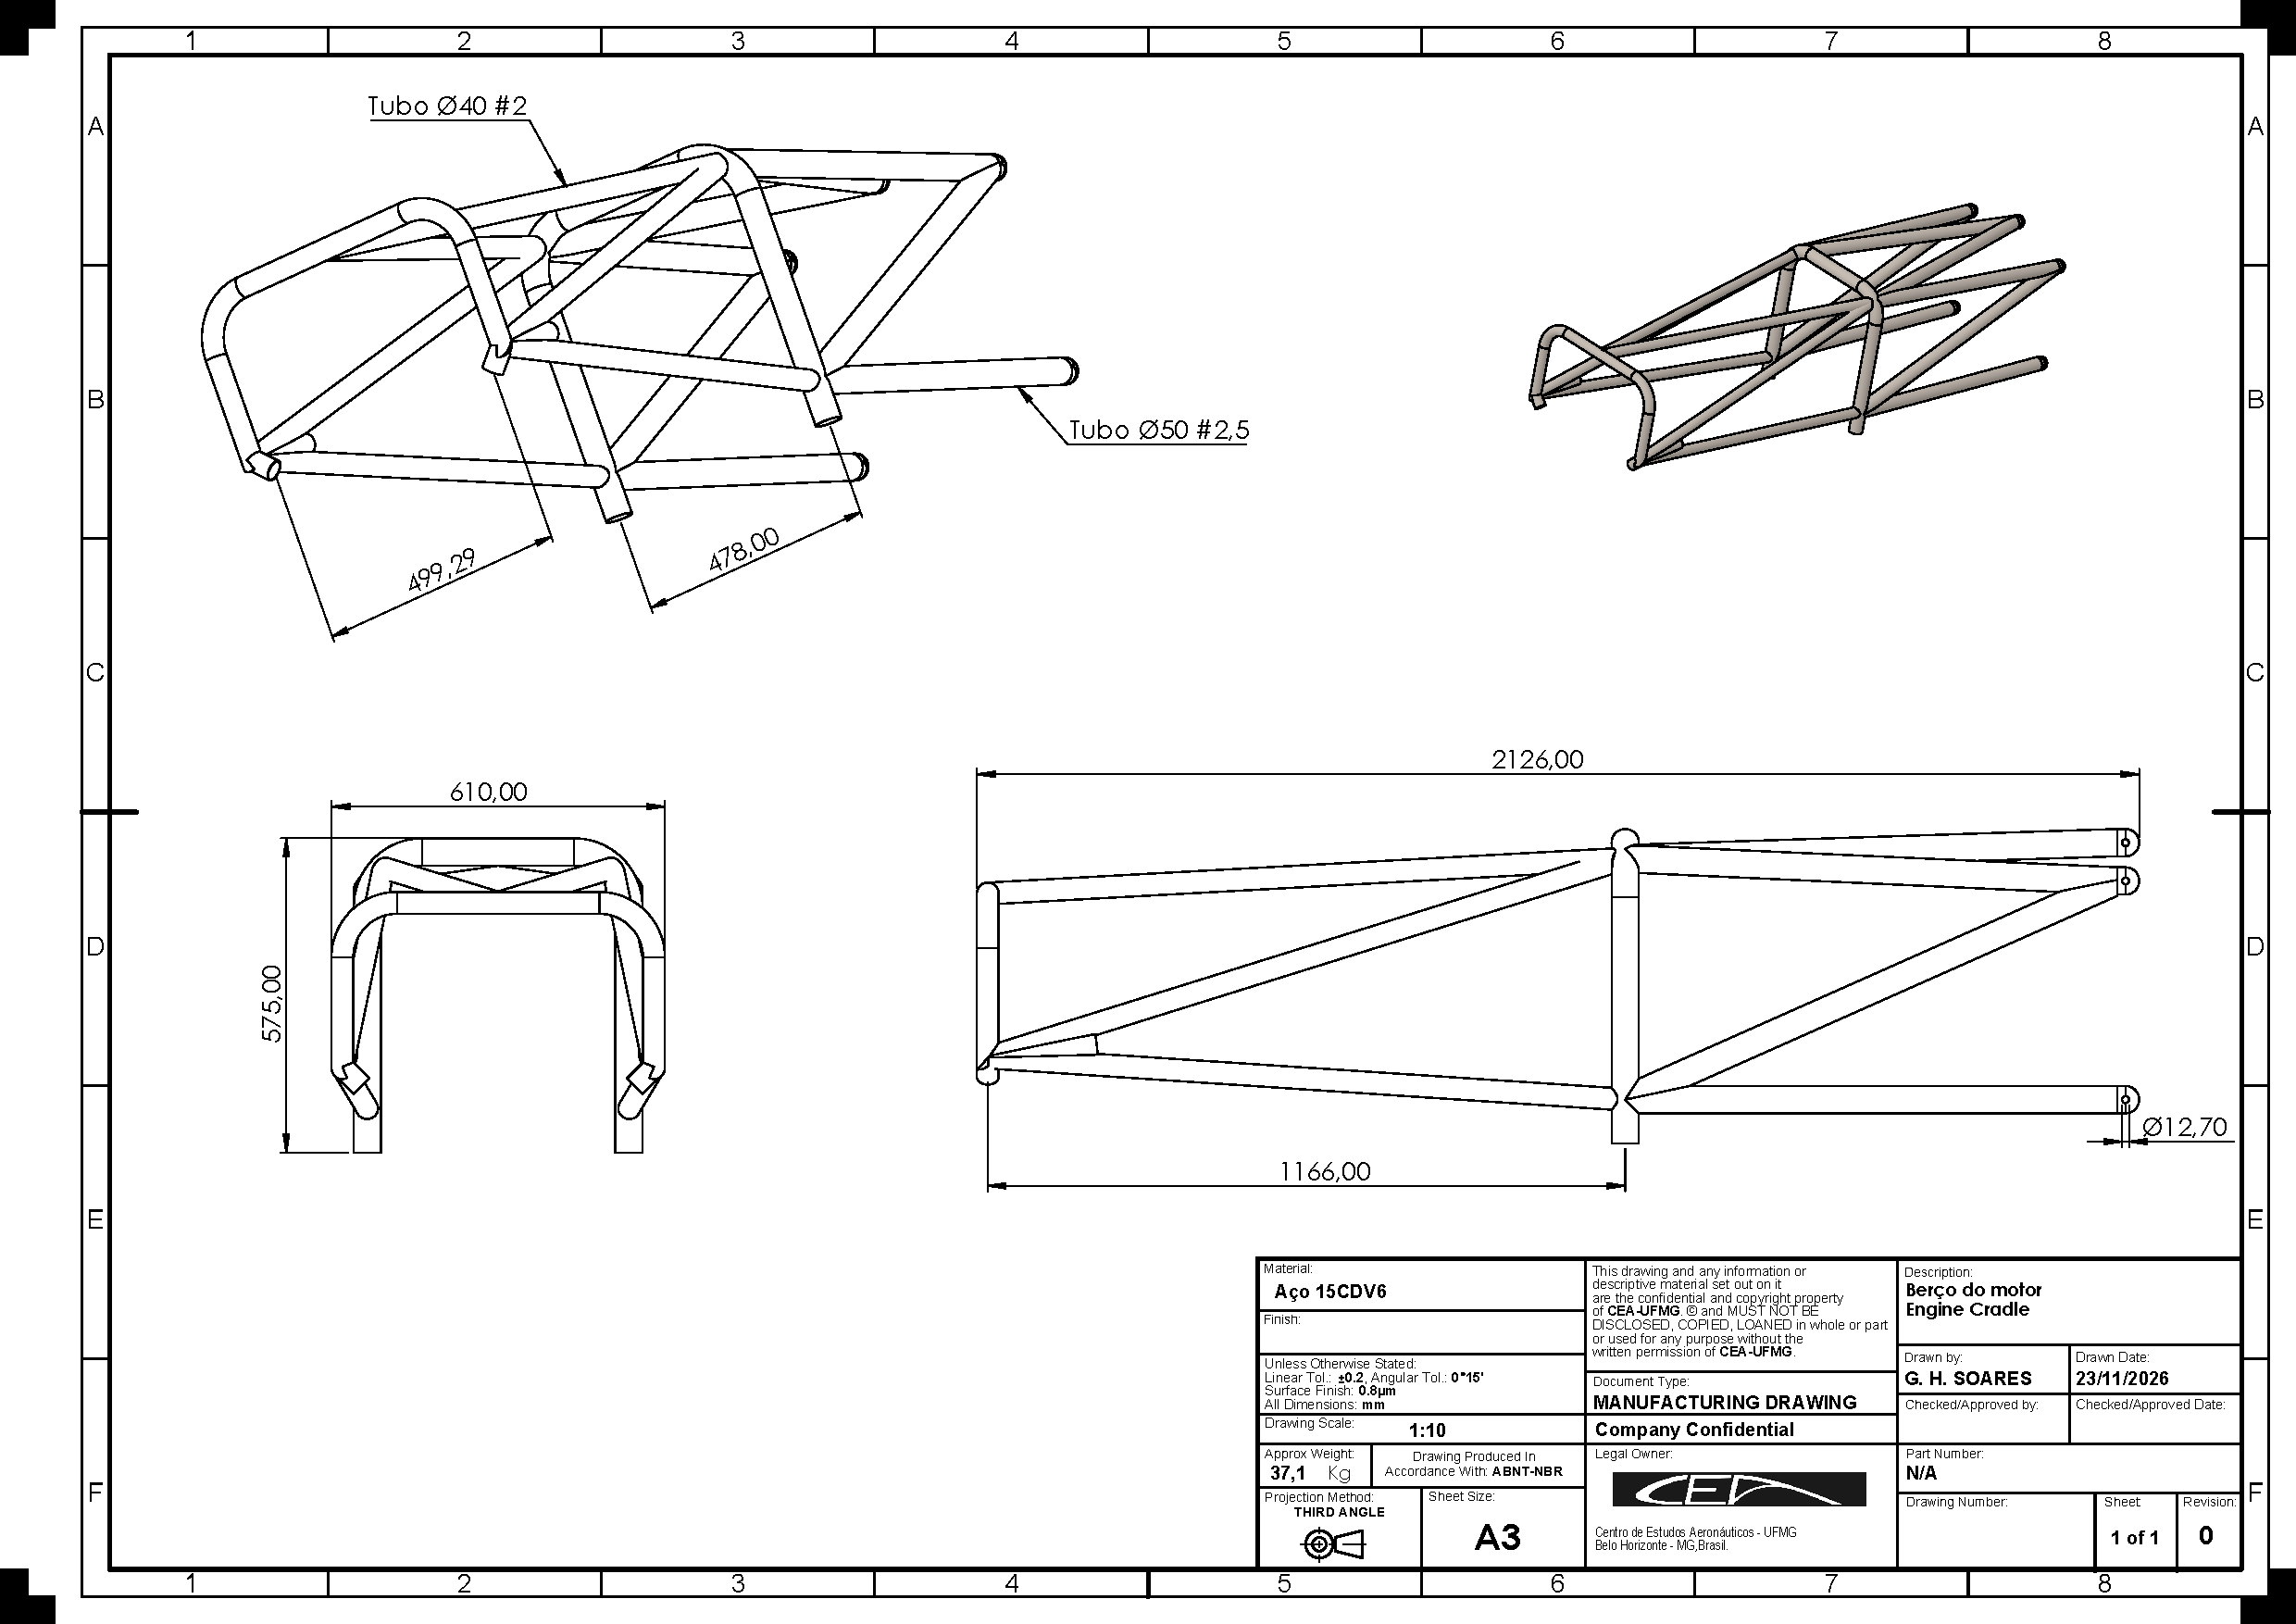
\includepdf[pages=-, angle=90]{berco.pdf}



\bibliography{referencias}
\bibliographystyle{ieeetr}

\end{document}